\documentclass[twoside]{book}

% Packages required by doxygen
\usepackage{fixltx2e}
\usepackage{calc}
\usepackage{doxygen}
\usepackage[export]{adjustbox} % also loads graphicx
\usepackage{graphicx}
\usepackage[utf8]{inputenc}
\usepackage{makeidx}
\usepackage{multicol}
\usepackage{multirow}
\PassOptionsToPackage{warn}{textcomp}
\usepackage{textcomp}
\usepackage[nointegrals]{wasysym}
\usepackage[table]{xcolor}

% Font selection
\usepackage[T1]{fontenc}
\usepackage[scaled=.90]{helvet}
\usepackage{courier}
\usepackage{amssymb}
\usepackage{sectsty}
\renewcommand{\familydefault}{\sfdefault}
\allsectionsfont{%
  \fontseries{bc}\selectfont%
  \color{darkgray}%
}
\renewcommand{\DoxyLabelFont}{%
  \fontseries{bc}\selectfont%
  \color{darkgray}%
}
\newcommand{\+}{\discretionary{\mbox{\scriptsize$\hookleftarrow$}}{}{}}

% Page & text layout
\usepackage{geometry}
\geometry{%
  a4paper,%
  top=2.5cm,%
  bottom=2.5cm,%
  left=2.5cm,%
  right=2.5cm%
}
\tolerance=750
\hfuzz=15pt
\hbadness=750
\setlength{\emergencystretch}{15pt}
\setlength{\parindent}{0cm}
\setlength{\parskip}{3ex plus 2ex minus 2ex}
\makeatletter
\renewcommand{\paragraph}{%
  \@startsection{paragraph}{4}{0ex}{-1.0ex}{1.0ex}{%
    \normalfont\normalsize\bfseries\SS@parafont%
  }%
}
\renewcommand{\subparagraph}{%
  \@startsection{subparagraph}{5}{0ex}{-1.0ex}{1.0ex}{%
    \normalfont\normalsize\bfseries\SS@subparafont%
  }%
}
\makeatother

% Headers & footers
\usepackage{fancyhdr}
\pagestyle{fancyplain}
\fancyhead[LE]{\fancyplain{}{\bfseries\thepage}}
\fancyhead[CE]{\fancyplain{}{}}
\fancyhead[RE]{\fancyplain{}{\bfseries\leftmark}}
\fancyhead[LO]{\fancyplain{}{\bfseries\rightmark}}
\fancyhead[CO]{\fancyplain{}{}}
\fancyhead[RO]{\fancyplain{}{\bfseries\thepage}}
\fancyfoot[LE]{\fancyplain{}{}}
\fancyfoot[CE]{\fancyplain{}{}}
\fancyfoot[RE]{\fancyplain{}{\bfseries\scriptsize Generated by Doxygen }}
\fancyfoot[LO]{\fancyplain{}{\bfseries\scriptsize Generated by Doxygen }}
\fancyfoot[CO]{\fancyplain{}{}}
\fancyfoot[RO]{\fancyplain{}{}}
\renewcommand{\footrulewidth}{0.4pt}
\renewcommand{\chaptermark}[1]{%
  \markboth{#1}{}%
}
\renewcommand{\sectionmark}[1]{%
  \markright{\thesection\ #1}%
}

% Indices & bibliography
\usepackage{natbib}
\usepackage[titles]{tocloft}
\setcounter{tocdepth}{3}
\setcounter{secnumdepth}{5}
\makeindex

% Hyperlinks (required, but should be loaded last)
\usepackage{ifpdf}
\ifpdf
  \usepackage[pdftex,pagebackref=true]{hyperref}
\else
  \usepackage[ps2pdf,pagebackref=true]{hyperref}
\fi
\hypersetup{%
  colorlinks=true,%
  linkcolor=blue,%
  citecolor=blue,%
  unicode%
}

% Custom commands
\newcommand{\clearemptydoublepage}{%
  \newpage{\pagestyle{empty}\cleardoublepage}%
}

\usepackage{caption}
\captionsetup{labelsep=space,justification=centering,font={bf},singlelinecheck=off,skip=4pt,position=top}

%===== C O N T E N T S =====

\begin{document}

% Titlepage & ToC
\hypersetup{pageanchor=false,
             bookmarksnumbered=true,
             pdfencoding=unicode
            }
\pagenumbering{alph}
\begin{titlepage}
\vspace*{7cm}
\begin{center}%
{\Large Library\+Core \\[1ex]\large 0.\+1.\+13 }\\
\vspace*{1cm}
{\large Generated by Doxygen 1.8.13}\\
\end{center}
\end{titlepage}
\clearemptydoublepage
\pagenumbering{roman}
\tableofcontents
\clearemptydoublepage
\pagenumbering{arabic}
\hypersetup{pageanchor=true}

%--- Begin generated contents ---
\chapter{Library \+:\+: Core}
\label{index}\hypertarget{index}{}Fundamental types, containers and utilities.

\href{https://travis-ci.com/open-space-collective/library-core}{\tt } \href{https://codecov.io/gh/open-space-collective/library-core}{\tt } \href{https://open-space-collective.github.io/library-core}{\tt }

\subsection*{Warning}

Library {\bfseries name} and {\bfseries license} are yet to be defined.

Please check the following projects\+:


\begin{DoxyItemize}
\item \href{https://github.com/orgs/open-space-collective/projects/1}{\tt Naming Project}
\item \href{https://github.com/orgs/open-space-collective/projects/2}{\tt Licensing Project}
\end{DoxyItemize}

{\itshape ⚠ This library is still under heavy development. Do not use!}

\subsection*{Structure}

The {\bfseries Core} library exhibits the following structure\+:


\begin{DoxyCode}
├── Types
│   ├── Integer
│   ├── Real
│   ├── String
│   ├── \hyperlink{namespacelibrary_1_1core_1_1types_ae37635b89098069fb3b8c5181edd0945}{Byte}
│   ├── \hyperlink{namespacelibrary_1_1core_1_1types_ae37635b89098069fb3b8c5181edd0945}{Byte} Array
│   ├── \hyperlink{namespacelibrary_1_1core_1_1types_ad87eeb821d7067ec94e06ed1980d6350}{Index}
│   ├── \hyperlink{namespacelibrary_1_1core_1_1types_a701626ea1027888ebbb8cfd0ff7adab0}{Size}
│   ├── \hyperlink{namespacelibrary_1_1core_1_1types_a06d9eaa410d43a0fa3f383040618e87d}{Sign}
│   ├── \hyperlink{namespacelibrary_1_1core_1_1types_ac12d38691838fbc9a36765ee62ace52a}{Unique}
│   ├── \hyperlink{namespacelibrary_1_1core_1_1types_a3dae1a00f899bac0366794fa85eda8ee}{Shared}
│   └── \hyperlink{namespacelibrary_1_1core_1_1types_a26c13c272f9fba4ce17ee4980be6703c}{Weak}
├── Containers
│   ├── Array
│   ├── \hyperlink{namespacelibrary_1_1core_1_1ctnr_a87ccf40619002299b341a5e76e989912}{List}
│   ├── \hyperlink{namespacelibrary_1_1core_1_1ctnr_a248e088a0b4ec44aff451a5c3663dcee}{Map}
│   ├── Ordered \hyperlink{namespacelibrary_1_1core_1_1ctnr_a248e088a0b4ec44aff451a5c3663dcee}{Map}
│   ├── Object
│   ├── Dictionary
│   ├── \hyperlink{namespacelibrary_1_1core_1_1ctnr_aad6f8de4c0f279c10436d59d4ace74bd}{Pair}
│   ├── Triple
│   ├── \hyperlink{namespacelibrary_1_1core_1_1ctnr_a551ef72e2adb570c4d6bdf5e1bbc96b9}{Tuple}
│   ├── Table
│   ├── Queue
│   ├── Stack
│   ├── Graph
│   └── Tree
├── File System
│   ├── Path
│   ├── File
│   ├── Directory
│   ├── Symbolic Link
│   └── Permission
├── System
│   ├── User
│   ├── Group
│   ├── CPU
│   ├── Memory
│   ├── Disk
│   └── Process
├── Logger
├── \hyperlink{namespacelibrary_1_1core_1_1logger_a35f71353edf64f68f7fe3874b01abaa8a902b0d55fddef6f8d651fe1035b7d4bd}{Error}
│   ├── Exception
│   ├── Runtime \hyperlink{namespacelibrary_1_1core_1_1logger_a35f71353edf64f68f7fe3874b01abaa8a902b0d55fddef6f8d651fe1035b7d4bd}{Error}
│   └── Runtime
│       ├── \hyperlink{namespacelibrary_1_1core_1_1types_a06d9eaa410d43a0fa3f383040618e87daec0fc0100c4fc1ce4eea230c3dc10360}{Undefined}
│       ├── Wrong
│       └── To Be Implemented
└── Utilities
    ├── Iterators
    └── Version
\end{DoxyCode}


\subsection*{Documentation}

The documentation can be found \href{https://open-space-collective.github.io/library-core}{\tt here}.

\subsection*{Setup}

\subsubsection*{Development}

Using \href{https://www.docker.com}{\tt Docker} is recommended, as the development tools and dependencies setup is described in the provided \href{./tools/development/docker/Dockerfile}{\tt Dockerfile}.

Instructions to install Docker can be found \href{https://docs.docker.com/install/}{\tt here}.

Start the development environment\+:


\begin{DoxyCode}
./tools/development/start.sh
\end{DoxyCode}


This will also build the {\ttfamily openspacecollective/library-\/core\+:latest} Docker image, if not present already.

If installing Docker is not an option, please manually install the development tools (G\+CC, C\+Make) and the dependencies. The procedure should be similar to the one described in the \href{./tools/development/docker/Dockerfile}{\tt Dockerfile}.

\subsubsection*{Build}

From the development environment\+:


\begin{DoxyCode}
./build.sh
\end{DoxyCode}


Manually\+:


\begin{DoxyCode}
mkdir -p build
cd build
cmake ..
make
\end{DoxyCode}


\subsubsection*{Test}

From the development environment\+:


\begin{DoxyCode}
./test.sh
\end{DoxyCode}


Manually\+:


\begin{DoxyCode}
./bin/library-core.test
\end{DoxyCode}


\subsection*{Dependencies}

The {\bfseries Core} library internally uses the following dependencies\+:

\tabulinesep=1mm
\begin{longtabu} spread 0pt [c]{*{4}{|X[-1]}|}
\hline
\rowcolor{\tableheadbgcolor}\textbf{ Name }&\textbf{ Version }&\textbf{ License }&\textbf{ Link  }\\\cline{1-4}
\endfirsthead
\hline
\endfoot
\hline
\rowcolor{\tableheadbgcolor}\textbf{ Name }&\textbf{ Version }&\textbf{ License }&\textbf{ Link  }\\\cline{1-4}
\endhead
Boost &1.\+67.\+0 &Boost Software License &\href{https://www.boost.org}{\tt boost.\+org} \\\cline{1-4}
Rapid\+J\+S\+ON &master &M\+IT &\href{http://rapidjson.org}{\tt rapidjson.\+org} \\\cline{1-4}
ordered-\/map &master &M\+IT &\href{https://github.com/Tessil/ordered-map}{\tt github.\+com/\+Tessil/ordered-\/map} \\\cline{1-4}
\{fmt\} &master &B\+S\+D-\/2-\/\+Clause &\href{https://github.com/fmtlib/fmt}{\tt github.\+com/fmtlib/fmt} \\\cline{1-4}
Rapidcsv &master &B\+S\+D-\/3-\/\+Clause &\href{https://github.com/d99kris/rapidcsv}{\tt github.\+com/d99kris/rapidcsv} \\\cline{1-4}
\end{longtabu}
\subsection*{Contribution}

Contributions are more than welcome!

Please read our \hyperlink{_c_o_n_t_r_i_b_u_t_i_n_g_8md}{contributing guide} to learn about our development process, how to propose fixes and improvements, and how to build and test the code.

\subsection*{Special Thanks}

{\itshape To be completed...}

\subsection*{License}

{\itshape To be defined...} 
\chapter{Contributing}
\label{md__c_o_n_t_r_i_b_u_t_i_n_g}
\Hypertarget{md__c_o_n_t_r_i_b_u_t_i_n_g}
{\itshape ⚠ This document is a work in progress.}\hypertarget{md__c_o_n_t_r_i_b_u_t_i_n_g_Introduction}{}\section{Introduction}\label{md__c_o_n_t_r_i_b_u_t_i_n_g_Introduction}
{\itshape To be completed...}\hypertarget{md__c_o_n_t_r_i_b_u_t_i_n_g_Guidelines}{}\section{Guidelines}\label{md__c_o_n_t_r_i_b_u_t_i_n_g_Guidelines}
\hypertarget{md__c_o_n_t_r_i_b_u_t_i_n_g_Codebase}{}\subsection{Codebase}\label{md__c_o_n_t_r_i_b_u_t_i_n_g_Codebase}
\hypertarget{md__c_o_n_t_r_i_b_u_t_i_n_g_C}{}\subsubsection{C++}\label{md__c_o_n_t_r_i_b_u_t_i_n_g_C}
Include order from specific to generic\+:


\begin{DoxyCode}{0}
\DoxyCodeLine{\textcolor{preprocessor}{\#include <Library/Astrodynamics/Orbit.hpp>}}
\DoxyCodeLine{}
\DoxyCodeLine{\textcolor{preprocessor}{\#include <\mbox{\hyperlink{_integer_8hpp}{Library/Core/Types/Integer.hpp}}>}}
\DoxyCodeLine{\textcolor{preprocessor}{\#include <\mbox{\hyperlink{_utilities_8hpp}{Library/Core/Utilities.hpp}}>}}
\DoxyCodeLine{}
\DoxyCodeLine{\textcolor{preprocessor}{\#include <map>}}
\DoxyCodeLine{\textcolor{preprocessor}{\#include <string>}}
\end{DoxyCode}


References\+:


\begin{DoxyItemize}
\item \href{https://stackoverflow.com/questions/2762568/c-c-include-file-order-best-practices}{\texttt{ https\+://stackoverflow.\+com/questions/2762568/c-\/c-\/include-\/file-\/order-\/best-\/practices}}
\item \href{https://blog.kowalczyk.info/article/qg/order-of-include-headers-in-cc.html}{\texttt{ https\+://blog.\+kowalczyk.\+info/article/qg/order-\/of-\/include-\/headers-\/in-\/cc.\+html}}
\end{DoxyItemize}\hypertarget{md__c_o_n_t_r_i_b_u_t_i_n_g_Python}{}\subsubsection{Python}\label{md__c_o_n_t_r_i_b_u_t_i_n_g_Python}
{\itshape To be completed...}\hypertarget{md__c_o_n_t_r_i_b_u_t_i_n_g_Version}{}\subsection{Version Control}\label{md__c_o_n_t_r_i_b_u_t_i_n_g_Version}
\hypertarget{md__c_o_n_t_r_i_b_u_t_i_n_g_Rules}{}\subsubsection{Rules}\label{md__c_o_n_t_r_i_b_u_t_i_n_g_Rules}
{\itshape To be completed...}\hypertarget{md__c_o_n_t_r_i_b_u_t_i_n_g_Commit}{}\subsubsection{Commit Messages}\label{md__c_o_n_t_r_i_b_u_t_i_n_g_Commit}
\href{https://chris.beams.io/posts/git-commit/}{\texttt{ How to Write a Git Commit Message}}

Use active form ({\ttfamily Do something}).

Prefix commit messages using the following tags\+:


\begin{DoxyItemize}
\item \mbox{[}feature\mbox{]}
\item \mbox{[}fix\mbox{]}
\item \mbox{[}misc\mbox{]}
\end{DoxyItemize}

Examples\+:


\begin{DoxyCode}{0}
\DoxyCodeLine{[feature] Implement high fidelity orbit propagator}
\end{DoxyCode}



\begin{DoxyCode}{0}
\DoxyCodeLine{[fix] Segmentation fault when fetching ephemeris data}
\end{DoxyCode}
\hypertarget{md__c_o_n_t_r_i_b_u_t_i_n_g_CodeOfConduct}{}\section{Code of Conduct}\label{md__c_o_n_t_r_i_b_u_t_i_n_g_CodeOfConduct}
{\itshape To be completed...} 
\chapter{Tutorial}
\label{md_docs__tutorial}
\Hypertarget{md_docs__tutorial}
Below are examples illustrating a few common use-\/cases.\hypertarget{md_docs__tutorial_Setup}{}\section{Setup}\label{md_docs__tutorial_Setup}
{\itshape To be completed...}\hypertarget{md_docs__tutorial_Examples}{}\section{Examples}\label{md_docs__tutorial_Examples}
\hypertarget{md_docs__tutorial_JSON}{}\subsection{Load / Write J\+S\+ON}\label{md_docs__tutorial_JSON}
\href{https://en.wikipedia.org/wiki/JSON}{\texttt{ J\+S\+ON}} is a great format for configuring applications and for exchanging data over the internet\+:

Assuming an {\ttfamily input.\+json} file as follows\+:


\begin{DoxyCode}{0}
\DoxyCodeLine{\{}
\DoxyCodeLine{    "Key 1": "Hello World!"}
\DoxyCodeLine{\}}
\end{DoxyCode}


the following code\+:


\begin{DoxyCode}{0}
\DoxyCodeLine{\textcolor{comment}{// Setup JSON file}}
\DoxyCodeLine{}
\DoxyCodeLine{File jsonFile = File::Path(Path::String(\textcolor{stringliteral}{"/path/to/input.json"})) ;}
\DoxyCodeLine{}
\DoxyCodeLine{\textcolor{comment}{// Create object by loading JSON file}}
\DoxyCodeLine{}
\DoxyCodeLine{Object \textcolor{keywordtype}{object} = Object::Load(jsonFile) ;}
\DoxyCodeLine{}
\DoxyCodeLine{\textcolor{comment}{// Get object value}}
\DoxyCodeLine{}
\DoxyCodeLine{String value = \textcolor{keywordtype}{object}[\textcolor{stringliteral}{"Key 1"}].toString() ; \textcolor{comment}{// "Hello World!"}}
\DoxyCodeLine{}
\DoxyCodeLine{\textcolor{comment}{// Set object value}}
\DoxyCodeLine{}
\DoxyCodeLine{\textcolor{keywordtype}{object}[\textcolor{stringliteral}{"Key 2"}] = Object::Integer(123) ;}
\DoxyCodeLine{}
\DoxyCodeLine{\textcolor{comment}{// Save object}}
\DoxyCodeLine{}
\DoxyCodeLine{\textcolor{keywordtype}{object}.writeToFile(File::Path(Path::String(\textcolor{stringliteral}{"/path/to/output.json"}))) ;}
\end{DoxyCode}


will return an {\ttfamily output.\+json} file as\+:


\begin{DoxyCode}{0}
\DoxyCodeLine{\{}
\DoxyCodeLine{    "Key 1": "Hello World!",}
\DoxyCodeLine{    "Key 2": 123}
\DoxyCodeLine{\}}
\end{DoxyCode}
 
\chapter{Namespace Index}
\section{Namespace List}
Here is a list of all namespaces with brief descriptions\+:\begin{DoxyCompactList}
\item\contentsline{section}{\mbox{\hyperlink{namespacelibrary}{library}} }{\pageref{namespacelibrary}}{}
\item\contentsline{section}{\mbox{\hyperlink{namespacelibrary_1_1core}{library\+::core}} }{\pageref{namespacelibrary_1_1core}}{}
\item\contentsline{section}{\mbox{\hyperlink{namespacelibrary_1_1core_1_1ctnr}{library\+::core\+::ctnr}} }{\pageref{namespacelibrary_1_1core_1_1ctnr}}{}
\item\contentsline{section}{\mbox{\hyperlink{namespacelibrary_1_1core_1_1ctnr_1_1iterators}{library\+::core\+::ctnr\+::iterators}} }{\pageref{namespacelibrary_1_1core_1_1ctnr_1_1iterators}}{}
\item\contentsline{section}{\mbox{\hyperlink{namespacelibrary_1_1core_1_1ctnr_1_1table}{library\+::core\+::ctnr\+::table}} }{\pageref{namespacelibrary_1_1core_1_1ctnr_1_1table}}{}
\item\contentsline{section}{\mbox{\hyperlink{namespacelibrary_1_1core_1_1error}{library\+::core\+::error}} }{\pageref{namespacelibrary_1_1core_1_1error}}{}
\item\contentsline{section}{\mbox{\hyperlink{namespacelibrary_1_1core_1_1error_1_1runtime}{library\+::core\+::error\+::runtime}} }{\pageref{namespacelibrary_1_1core_1_1error_1_1runtime}}{}
\item\contentsline{section}{\mbox{\hyperlink{namespacelibrary_1_1core_1_1fs}{library\+::core\+::fs}} }{\pageref{namespacelibrary_1_1core_1_1fs}}{}
\item\contentsline{section}{\mbox{\hyperlink{namespacelibrary_1_1core_1_1logger}{library\+::core\+::logger}} }{\pageref{namespacelibrary_1_1core_1_1logger}}{}
\item\contentsline{section}{\mbox{\hyperlink{namespacelibrary_1_1core_1_1logger_1_1sinks}{library\+::core\+::logger\+::sinks}} }{\pageref{namespacelibrary_1_1core_1_1logger_1_1sinks}}{}
\item\contentsline{section}{\mbox{\hyperlink{namespacelibrary_1_1core_1_1logger_1_1sources}{library\+::core\+::logger\+::sources}} }{\pageref{namespacelibrary_1_1core_1_1logger_1_1sources}}{}
\item\contentsline{section}{\mbox{\hyperlink{namespacelibrary_1_1core_1_1system}{library\+::core\+::system}} }{\pageref{namespacelibrary_1_1core_1_1system}}{}
\item\contentsline{section}{\mbox{\hyperlink{namespacelibrary_1_1core_1_1types}{library\+::core\+::types}} }{\pageref{namespacelibrary_1_1core_1_1types}}{}
\item\contentsline{section}{\mbox{\hyperlink{namespacelibrary_1_1core_1_1utils}{library\+::core\+::utils}} }{\pageref{namespacelibrary_1_1core_1_1utils}}{}
\end{DoxyCompactList}

\chapter{Hierarchical Index}
\section{Class Hierarchy}
This inheritance list is sorted roughly, but not completely, alphabetically\+:\begin{DoxyCompactList}
\item std\+:\+:basic\+\_\+string$<$ Char $>$\begin{DoxyCompactList}
\item std\+:\+:string\begin{DoxyCompactList}
\item \contentsline{section}{library\+:\+:core\+:\+:types\+:\+:String}{\pageref{classlibrary_1_1core_1_1types_1_1String}}{}
\end{DoxyCompactList}
\end{DoxyCompactList}
\item \contentsline{section}{library\+:\+:core\+:\+:types\+:\+:Byte\+Array}{\pageref{classlibrary_1_1core_1_1types_1_1ByteArray}}{}
\item \contentsline{section}{library\+:\+:core\+:\+:ctnr\+:\+:Dictionary\+:\+:Const\+Iterator}{\pageref{classlibrary_1_1core_1_1ctnr_1_1Dictionary_1_1ConstIterator}}{}
\item \contentsline{section}{library\+:\+:core\+:\+:ctnr\+:\+:Dictionary}{\pageref{classlibrary_1_1core_1_1ctnr_1_1Dictionary}}{}
\item \contentsline{section}{library\+:\+:core\+:\+:fs\+:\+:Directory}{\pageref{classlibrary_1_1core_1_1fs_1_1Directory}}{}
\item \contentsline{section}{Eigen\+Matrix\+From\+Python$<$ Mat\+Type $>$}{\pageref{structEigenMatrixFromPython}}{}
\item \contentsline{section}{Eigen\+Matrix\+To\+Python$<$ Mat\+Type $>$}{\pageref{structEigenMatrixToPython}}{}
\item Environment\begin{DoxyCompactList}
\item \contentsline{section}{library\+:\+:core\+:\+:test\+:\+:Environment}{\pageref{classlibrary_1_1core_1_1test_1_1Environment}}{}
\end{DoxyCompactList}
\item std\+:\+:exception\begin{DoxyCompactList}
\item \contentsline{section}{library\+:\+:core\+:\+:error\+:\+:Exception}{\pageref{classlibrary_1_1core_1_1error_1_1Exception}}{}
\begin{DoxyCompactList}
\item \contentsline{section}{library\+:\+:core\+:\+:error\+:\+:Runtime\+Error}{\pageref{classlibrary_1_1core_1_1error_1_1RuntimeError}}{}
\begin{DoxyCompactList}
\item \contentsline{section}{library\+:\+:core\+:\+:error\+:\+:runtime\+:\+:To\+Be\+Implemented}{\pageref{classlibrary_1_1core_1_1error_1_1runtime_1_1ToBeImplemented}}{}
\item \contentsline{section}{library\+:\+:core\+:\+:error\+:\+:runtime\+:\+:Undefined}{\pageref{classlibrary_1_1core_1_1error_1_1runtime_1_1Undefined}}{}
\item \contentsline{section}{library\+:\+:core\+:\+:error\+:\+:runtime\+:\+:Wrong}{\pageref{classlibrary_1_1core_1_1error_1_1runtime_1_1Wrong}}{}
\end{DoxyCompactList}
\end{DoxyCompactList}
\end{DoxyCompactList}
\item \contentsline{section}{library\+:\+:core\+:\+:fs\+:\+:File}{\pageref{classlibrary_1_1core_1_1fs_1_1File}}{}
\item \contentsline{section}{library\+:\+:core\+:\+:ctnr\+:\+:Graph}{\pageref{classlibrary_1_1core_1_1ctnr_1_1Graph}}{}
\item \contentsline{section}{library\+:\+:core\+:\+:system\+:\+:Group}{\pageref{classlibrary_1_1core_1_1system_1_1Group}}{}
\item \contentsline{section}{library\+:\+:core\+:\+:types\+:\+:Has\+Get\+String$<$ T $>$}{\pageref{classlibrary_1_1core_1_1types_1_1HasGetString}}{}
\item \contentsline{section}{std\+:\+:hash$<$ library\+:\+:core\+:\+:types\+:\+:String $>$}{\pageref{structstd_1_1hash_3_01library_1_1core_1_1types_1_1String_01_4}}{}
\item \contentsline{section}{library\+:\+:core\+:\+:types\+:\+:Integer}{\pageref{classlibrary_1_1core_1_1types_1_1Integer}}{}
\item \contentsline{section}{library\+:\+:core\+:\+:ctnr\+:\+:Dictionary\+:\+:Iterator}{\pageref{classlibrary_1_1core_1_1ctnr_1_1Dictionary_1_1Iterator}}{}
\item \contentsline{section}{library\+:\+:core\+:\+:utils\+:\+:Print\+:\+:Line\+Buffer}{\pageref{classlibrary_1_1core_1_1utils_1_1Print_1_1LineBuffer}}{}
\item \contentsline{section}{library\+:\+:core\+:\+:Logger}{\pageref{classlibrary_1_1core_1_1Logger}}{}
\item \contentsline{section}{Numpy\+Equivalent\+Type$<$ S\+C\+A\+L\+AR $>$}{\pageref{structNumpyEquivalentType}}{}
\item \contentsline{section}{Numpy\+Equivalent\+Type$<$ double $>$}{\pageref{structNumpyEquivalentType_3_01double_01_4}}{}
\item \contentsline{section}{Numpy\+Equivalent\+Type$<$ float $>$}{\pageref{structNumpyEquivalentType_3_01float_01_4}}{}
\item \contentsline{section}{Numpy\+Equivalent\+Type$<$ int $>$}{\pageref{structNumpyEquivalentType_3_01int_01_4}}{}
\item \contentsline{section}{Numpy\+Equivalent\+Type$<$ std\+:\+:complex$<$ double $>$ $>$}{\pageref{structNumpyEquivalentType_3_01std_1_1complex_3_01double_01_4_01_4}}{}
\item \contentsline{section}{library\+:\+:core\+:\+:ctnr\+:\+:Object}{\pageref{classlibrary_1_1core_1_1ctnr_1_1Object}}{}
\item \contentsline{section}{library\+:\+:core\+:\+:fs\+:\+:Path}{\pageref{classlibrary_1_1core_1_1fs_1_1Path}}{}
\item \contentsline{section}{library\+:\+:core\+:\+:fs\+:\+:Permission\+Set}{\pageref{classlibrary_1_1core_1_1fs_1_1PermissionSet}}{}
\item \contentsline{section}{library\+:\+:core\+:\+:utils\+:\+:Print}{\pageref{classlibrary_1_1core_1_1utils_1_1Print}}{}
\item \contentsline{section}{library\+:\+:core\+:\+:logger\+:\+:Pump}{\pageref{classlibrary_1_1core_1_1logger_1_1Pump}}{}
\item \contentsline{section}{library\+:\+:core\+:\+:ctnr\+:\+:Queue}{\pageref{classlibrary_1_1core_1_1ctnr_1_1Queue}}{}
\item \contentsline{section}{library\+:\+:core\+:\+:types\+:\+:Real}{\pageref{classlibrary_1_1core_1_1types_1_1Real}}{}
\item \contentsline{section}{library\+:\+:core\+:\+:logger\+:\+:Sink}{\pageref{classlibrary_1_1core_1_1logger_1_1Sink}}{}
\item \contentsline{section}{library\+:\+:core\+:\+:logger\+:\+:sinks\+:\+:Sink}{\pageref{classlibrary_1_1core_1_1logger_1_1sinks_1_1Sink}}{}
\begin{DoxyCompactList}
\item \contentsline{section}{library\+:\+:core\+:\+:logger\+:\+:sinks\+:\+:Console}{\pageref{classlibrary_1_1core_1_1logger_1_1sinks_1_1Console}}{}
\end{DoxyCompactList}
\item \contentsline{section}{library\+:\+:core\+:\+:logger\+:\+:Source}{\pageref{classlibrary_1_1core_1_1logger_1_1Source}}{}
\item \contentsline{section}{library\+:\+:core\+:\+:logger\+:\+:sources\+:\+:Source}{\pageref{classlibrary_1_1core_1_1logger_1_1sources_1_1Source}}{}
\item \contentsline{section}{library\+:\+:core\+:\+:ctnr\+:\+:Stack}{\pageref{classlibrary_1_1core_1_1ctnr_1_1Stack}}{}
\item \contentsline{section}{library\+:\+:core\+:\+:ctnr\+:\+:Table}{\pageref{classlibrary_1_1core_1_1ctnr_1_1Table}}{}
\item \contentsline{section}{Test\+Class}{\pageref{classTestClass}}{}
\item \contentsline{section}{library\+:\+:core\+:\+:ctnr\+:\+:Tree}{\pageref{classlibrary_1_1core_1_1ctnr_1_1Tree}}{}
\item \contentsline{section}{library\+:\+:core\+:\+:ctnr\+:\+:Triple$<$ T, U, V $>$}{\pageref{structlibrary_1_1core_1_1ctnr_1_1Triple}}{}
\item \contentsline{section}{library\+:\+:core\+:\+:system\+:\+:User}{\pageref{classlibrary_1_1core_1_1system_1_1User}}{}
\item std\+:\+:vector$<$ T $>$\begin{DoxyCompactList}
\item \contentsline{section}{library\+:\+:core\+:\+:ctnr\+:\+:Array$<$ Byte $>$}{\pageref{classlibrary_1_1core_1_1ctnr_1_1Array}}{}
\item \contentsline{section}{library\+:\+:core\+:\+:ctnr\+:\+:Array$<$ library\+:\+:core\+:\+:logger\+:\+:Sink $>$}{\pageref{classlibrary_1_1core_1_1ctnr_1_1Array}}{}
\item \contentsline{section}{library\+:\+:core\+:\+:ctnr\+:\+:Array$<$ library\+:\+:core\+:\+:types\+:\+:String $>$}{\pageref{classlibrary_1_1core_1_1ctnr_1_1Array}}{}
\item \contentsline{section}{library\+:\+:core\+:\+:ctnr\+:\+:Array$<$ T $>$}{\pageref{classlibrary_1_1core_1_1ctnr_1_1Array}}{}
\end{DoxyCompactList}
\end{DoxyCompactList}

\chapter{Class Index}
\section{Class List}
Here are the classes, structs, unions and interfaces with brief descriptions\+:\begin{DoxyCompactList}
\item\contentsline{section}{\hyperlink{classlibrary_1_1core_1_1ctnr_1_1_array}{library\+::core\+::ctnr\+::\+Array$<$ T $>$} \\*\hyperlink{classlibrary_1_1core_1_1ctnr_1_1_array}{Array} container }{\pageref{classlibrary_1_1core_1_1ctnr_1_1_array}}{}
\item\contentsline{section}{\hyperlink{classlibrary_1_1core_1_1types_1_1_byte_array}{library\+::core\+::types\+::\+Byte\+Array} \\*An array of bytes \mbox{[}T\+BI\mbox{]} }{\pageref{classlibrary_1_1core_1_1types_1_1_byte_array}}{}
\item\contentsline{section}{\hyperlink{classlibrary_1_1core_1_1logger_1_1sinks_1_1_console}{library\+::core\+::logger\+::sinks\+::\+Console} \\*Log console sink }{\pageref{classlibrary_1_1core_1_1logger_1_1sinks_1_1_console}}{}
\item\contentsline{section}{\hyperlink{classlibrary_1_1core_1_1ctnr_1_1_dictionary_1_1_const_iterator}{library\+::core\+::ctnr\+::\+Dictionary\+::\+Const\+Iterator} }{\pageref{classlibrary_1_1core_1_1ctnr_1_1_dictionary_1_1_const_iterator}}{}
\item\contentsline{section}{\hyperlink{classlibrary_1_1core_1_1ctnr_1_1_dictionary}{library\+::core\+::ctnr\+::\+Dictionary} \\*Key-\/value pairs container }{\pageref{classlibrary_1_1core_1_1ctnr_1_1_dictionary}}{}
\item\contentsline{section}{\hyperlink{classlibrary_1_1core_1_1fs_1_1_directory}{library\+::core\+::fs\+::\+Directory} \\*Cataloging structure which contains references to other computer files, and possibly other directories }{\pageref{classlibrary_1_1core_1_1fs_1_1_directory}}{}
\item\contentsline{section}{\hyperlink{classlibrary_1_1core_1_1error_1_1_exception}{library\+::core\+::error\+::\+Exception} \\*\hyperlink{classlibrary_1_1core_1_1error_1_1_exception}{Exception} class }{\pageref{classlibrary_1_1core_1_1error_1_1_exception}}{}
\item\contentsline{section}{\hyperlink{classlibrary_1_1core_1_1fs_1_1_file}{library\+::core\+::fs\+::\+File} \\*Computer resource for recording data discretely in a computer storage device }{\pageref{classlibrary_1_1core_1_1fs_1_1_file}}{}
\item\contentsline{section}{\hyperlink{classlibrary_1_1core_1_1ctnr_1_1_graph}{library\+::core\+::ctnr\+::\+Graph} \\*Structure consisting of a finite set of vertices, together with a set of pairs of these vertices (edges) }{\pageref{classlibrary_1_1core_1_1ctnr_1_1_graph}}{}
\item\contentsline{section}{\hyperlink{classlibrary_1_1core_1_1system_1_1_group}{library\+::core\+::system\+::\+Group} \\*\hyperlink{classlibrary_1_1core_1_1system_1_1_group}{Group} }{\pageref{classlibrary_1_1core_1_1system_1_1_group}}{}
\item\contentsline{section}{\hyperlink{classlibrary_1_1core_1_1types_1_1_has_get_string}{library\+::core\+::types\+::\+Has\+Get\+String$<$ T $>$} \\*https\+://gist.github.\+com/fenbf/d2cd670704b82e2ce7fd }{\pageref{classlibrary_1_1core_1_1types_1_1_has_get_string}}{}
\item\contentsline{section}{\hyperlink{classlibrary_1_1core_1_1types_1_1_integer}{library\+::core\+::types\+::\+Integer} \\*\hyperlink{classlibrary_1_1core_1_1types_1_1_integer}{Integer} type }{\pageref{classlibrary_1_1core_1_1types_1_1_integer}}{}
\item\contentsline{section}{\hyperlink{classlibrary_1_1core_1_1ctnr_1_1_dictionary_1_1_iterator}{library\+::core\+::ctnr\+::\+Dictionary\+::\+Iterator} }{\pageref{classlibrary_1_1core_1_1ctnr_1_1_dictionary_1_1_iterator}}{}
\item\contentsline{section}{\hyperlink{classlibrary_1_1core_1_1utils_1_1_print_1_1_line_buffer}{library\+::core\+::utils\+::\+Print\+::\+Line\+Buffer} }{\pageref{classlibrary_1_1core_1_1utils_1_1_print_1_1_line_buffer}}{}
\item\contentsline{section}{\hyperlink{classlibrary_1_1core_1_1_logger}{library\+::core\+::\+Logger} \\*Log management }{\pageref{classlibrary_1_1core_1_1_logger}}{}
\item\contentsline{section}{\hyperlink{classlibrary_1_1core_1_1ctnr_1_1_object}{library\+::core\+::ctnr\+::\+Object} \\*Universal type container }{\pageref{classlibrary_1_1core_1_1ctnr_1_1_object}}{}
\item\contentsline{section}{\hyperlink{classlibrary_1_1core_1_1fs_1_1_path}{library\+::core\+::fs\+::\+Path} }{\pageref{classlibrary_1_1core_1_1fs_1_1_path}}{}
\item\contentsline{section}{\hyperlink{classlibrary_1_1core_1_1fs_1_1_permission_set}{library\+::core\+::fs\+::\+Permission\+Set} \\*Permissions control the ability of the users to view, change, navigate, and execute the contents of the file system }{\pageref{classlibrary_1_1core_1_1fs_1_1_permission_set}}{}
\item\contentsline{section}{\hyperlink{classlibrary_1_1core_1_1utils_1_1_print}{library\+::core\+::utils\+::\+Print} }{\pageref{classlibrary_1_1core_1_1utils_1_1_print}}{}
\item\contentsline{section}{\hyperlink{classlibrary_1_1core_1_1logger_1_1_pump}{library\+::core\+::logger\+::\+Pump} \\*Log pump }{\pageref{classlibrary_1_1core_1_1logger_1_1_pump}}{}
\item\contentsline{section}{\hyperlink{classlibrary_1_1core_1_1ctnr_1_1_queue}{library\+::core\+::ctnr\+::\+Queue} \\*First-\/in, first-\/out (F\+I\+FO) container }{\pageref{classlibrary_1_1core_1_1ctnr_1_1_queue}}{}
\item\contentsline{section}{\hyperlink{classlibrary_1_1core_1_1types_1_1_real}{library\+::core\+::types\+::\+Real} \\*\hyperlink{classlibrary_1_1core_1_1types_1_1_real}{Real} type }{\pageref{classlibrary_1_1core_1_1types_1_1_real}}{}
\item\contentsline{section}{\hyperlink{classlibrary_1_1core_1_1error_1_1_runtime_error}{library\+::core\+::error\+::\+Runtime\+Error} \\*Runtime error class }{\pageref{classlibrary_1_1core_1_1error_1_1_runtime_error}}{}
\item\contentsline{section}{\hyperlink{classlibrary_1_1core_1_1logger_1_1_sink}{library\+::core\+::logger\+::\+Sink} \\*Log sink }{\pageref{classlibrary_1_1core_1_1logger_1_1_sink}}{}
\item\contentsline{section}{\hyperlink{classlibrary_1_1core_1_1logger_1_1sinks_1_1_sink}{library\+::core\+::logger\+::sinks\+::\+Sink} \\*Log sink base }{\pageref{classlibrary_1_1core_1_1logger_1_1sinks_1_1_sink}}{}
\item\contentsline{section}{\hyperlink{classlibrary_1_1core_1_1logger_1_1sources_1_1_source}{library\+::core\+::logger\+::sources\+::\+Source} \\*Log source base }{\pageref{classlibrary_1_1core_1_1logger_1_1sources_1_1_source}}{}
\item\contentsline{section}{\hyperlink{classlibrary_1_1core_1_1logger_1_1_source}{library\+::core\+::logger\+::\+Source} \\*Log source }{\pageref{classlibrary_1_1core_1_1logger_1_1_source}}{}
\item\contentsline{section}{\hyperlink{classlibrary_1_1core_1_1ctnr_1_1_stack}{library\+::core\+::ctnr\+::\+Stack} \\*First-\/in, last-\/out (F\+I\+LO) container }{\pageref{classlibrary_1_1core_1_1ctnr_1_1_stack}}{}
\item\contentsline{section}{\hyperlink{classlibrary_1_1core_1_1types_1_1_string}{library\+::core\+::types\+::\+String} \\*A sequence of characters }{\pageref{classlibrary_1_1core_1_1types_1_1_string}}{}
\item\contentsline{section}{\hyperlink{classlibrary_1_1core_1_1ctnr_1_1_table}{library\+::core\+::ctnr\+::\+Table} \\*\hyperlink{classlibrary_1_1core_1_1ctnr_1_1_table}{Table} container }{\pageref{classlibrary_1_1core_1_1ctnr_1_1_table}}{}
\item\contentsline{section}{\hyperlink{classlibrary_1_1core_1_1error_1_1runtime_1_1_to_be_implemented}{library\+::core\+::error\+::runtime\+::\+To\+Be\+Implemented} \\*To be implemented error class }{\pageref{classlibrary_1_1core_1_1error_1_1runtime_1_1_to_be_implemented}}{}
\item\contentsline{section}{\hyperlink{classlibrary_1_1core_1_1ctnr_1_1_tree}{library\+::core\+::ctnr\+::\+Tree} \\*Undirected graph in which any two vertices are connected by exactly one path }{\pageref{classlibrary_1_1core_1_1ctnr_1_1_tree}}{}
\item\contentsline{section}{\hyperlink{structlibrary_1_1core_1_1ctnr_1_1_triple}{library\+::core\+::ctnr\+::\+Triple$<$ T, U, V $>$} \\*\hyperlink{structlibrary_1_1core_1_1ctnr_1_1_triple}{Triple} container }{\pageref{structlibrary_1_1core_1_1ctnr_1_1_triple}}{}
\item\contentsline{section}{\hyperlink{classlibrary_1_1core_1_1error_1_1runtime_1_1_undefined}{library\+::core\+::error\+::runtime\+::\+Undefined} \\*\hyperlink{classlibrary_1_1core_1_1error_1_1runtime_1_1_undefined}{Undefined} variable error class }{\pageref{classlibrary_1_1core_1_1error_1_1runtime_1_1_undefined}}{}
\item\contentsline{section}{\hyperlink{classlibrary_1_1core_1_1system_1_1_user}{library\+::core\+::system\+::\+User} \\*\hyperlink{classlibrary_1_1core_1_1system_1_1_user}{User} }{\pageref{classlibrary_1_1core_1_1system_1_1_user}}{}
\item\contentsline{section}{\hyperlink{classlibrary_1_1core_1_1error_1_1runtime_1_1_wrong}{library\+::core\+::error\+::runtime\+::\+Wrong} \\*\hyperlink{classlibrary_1_1core_1_1error_1_1runtime_1_1_wrong}{Wrong} variable error class }{\pageref{classlibrary_1_1core_1_1error_1_1runtime_1_1_wrong}}{}
\end{DoxyCompactList}

\chapter{File Index}
\section{File List}
Here is a list of all files with brief descriptions\+:\begin{DoxyCompactList}
\item\contentsline{section}{include/\+Library/\+Core/\hyperlink{_error_8hpp}{Error.\+hpp} }{\pageref{_error_8hpp}}{}
\item\contentsline{section}{include/\+Library/\+Core/\hyperlink{_file_system_8hpp}{File\+System.\+hpp} }{\pageref{_file_system_8hpp}}{}
\item\contentsline{section}{include/\+Library/\+Core/\hyperlink{_logger_8hpp}{Logger.\+hpp} }{\pageref{_logger_8hpp}}{}
\item\contentsline{section}{include/\+Library/\+Core/\hyperlink{_program_8hpp}{Program.\+hpp} }{\pageref{_program_8hpp}}{}
\item\contentsline{section}{include/\+Library/\+Core/\hyperlink{_types_8hpp}{Types.\+hpp} }{\pageref{_types_8hpp}}{}
\item\contentsline{section}{include/\+Library/\+Core/\hyperlink{_utilities_8hpp}{Utilities.\+hpp} }{\pageref{_utilities_8hpp}}{}
\item\contentsline{section}{include/\+Library/\+Core/\+Containers/\hyperlink{_array_8hpp}{Array.\+hpp} }{\pageref{_array_8hpp}}{}
\item\contentsline{section}{include/\+Library/\+Core/\+Containers/\hyperlink{_dictionary_8hpp}{Dictionary.\+hpp} }{\pageref{_dictionary_8hpp}}{}
\item\contentsline{section}{include/\+Library/\+Core/\+Containers/\hyperlink{_graph_8hpp}{Graph.\+hpp} }{\pageref{_graph_8hpp}}{}
\item\contentsline{section}{include/\+Library/\+Core/\+Containers/\hyperlink{_list_8hpp}{List.\+hpp} }{\pageref{_list_8hpp}}{}
\item\contentsline{section}{include/\+Library/\+Core/\+Containers/\hyperlink{_map_8hpp}{Map.\+hpp} }{\pageref{_map_8hpp}}{}
\item\contentsline{section}{include/\+Library/\+Core/\+Containers/\hyperlink{_object_8hpp}{Object.\+hpp} }{\pageref{_object_8hpp}}{}
\item\contentsline{section}{include/\+Library/\+Core/\+Containers/\hyperlink{_ordered_map_8hpp}{Ordered\+Map.\+hpp} }{\pageref{_ordered_map_8hpp}}{}
\item\contentsline{section}{include/\+Library/\+Core/\+Containers/\hyperlink{_pair_8hpp}{Pair.\+hpp} }{\pageref{_pair_8hpp}}{}
\item\contentsline{section}{include/\+Library/\+Core/\+Containers/\hyperlink{_queue_8hpp}{Queue.\+hpp} }{\pageref{_queue_8hpp}}{}
\item\contentsline{section}{include/\+Library/\+Core/\+Containers/\hyperlink{_stack_8hpp}{Stack.\+hpp} }{\pageref{_stack_8hpp}}{}
\item\contentsline{section}{include/\+Library/\+Core/\+Containers/\hyperlink{_table_8hpp}{Table.\+hpp} }{\pageref{_table_8hpp}}{}
\item\contentsline{section}{include/\+Library/\+Core/\+Containers/\hyperlink{_tree_8hpp}{Tree.\+hpp} }{\pageref{_tree_8hpp}}{}
\item\contentsline{section}{include/\+Library/\+Core/\+Containers/\hyperlink{_triple_8hpp}{Triple.\+hpp} }{\pageref{_triple_8hpp}}{}
\item\contentsline{section}{include/\+Library/\+Core/\+Containers/\hyperlink{_tuple_8hpp}{Tuple.\+hpp} }{\pageref{_tuple_8hpp}}{}
\item\contentsline{section}{include/\+Library/\+Core/\+Containers/\+Iterators/\hyperlink{_zip_8hpp}{Zip.\+hpp} }{\pageref{_zip_8hpp}}{}
\item\contentsline{section}{include/\+Library/\+Core/\+Containers/\+Table/\hyperlink{_cell_8hpp}{Cell.\+hpp} }{\pageref{_cell_8hpp}}{}
\item\contentsline{section}{include/\+Library/\+Core/\+Containers/\+Table/\hyperlink{_row_8hpp}{Row.\+hpp} }{\pageref{_row_8hpp}}{}
\item\contentsline{section}{include/\+Library/\+Core/\+Error/\hyperlink{_exception_8hpp}{Exception.\+hpp} }{\pageref{_exception_8hpp}}{}
\item\contentsline{section}{include/\+Library/\+Core/\+Error/\hyperlink{_runtime_error_8hpp}{Runtime\+Error.\+hpp} }{\pageref{_runtime_error_8hpp}}{}
\item\contentsline{section}{include/\+Library/\+Core/\+Error/\+Runtime/\hyperlink{_to_be_implemented_8hpp}{To\+Be\+Implemented.\+hpp} }{\pageref{_to_be_implemented_8hpp}}{}
\item\contentsline{section}{include/\+Library/\+Core/\+Error/\+Runtime/\hyperlink{_undefined_8hpp}{Undefined.\+hpp} }{\pageref{_undefined_8hpp}}{}
\item\contentsline{section}{include/\+Library/\+Core/\+Error/\+Runtime/\hyperlink{_wrong_8hpp}{Wrong.\+hpp} }{\pageref{_wrong_8hpp}}{}
\item\contentsline{section}{include/\+Library/\+Core/\+File\+System/\hyperlink{_directory_8hpp}{Directory.\+hpp} }{\pageref{_directory_8hpp}}{}
\item\contentsline{section}{include/\+Library/\+Core/\+File\+System/\hyperlink{_file_8hpp}{File.\+hpp} }{\pageref{_file_8hpp}}{}
\item\contentsline{section}{include/\+Library/\+Core/\+File\+System/\hyperlink{_path_8hpp}{Path.\+hpp} }{\pageref{_path_8hpp}}{}
\item\contentsline{section}{include/\+Library/\+Core/\+File\+System/\hyperlink{_permission_set_8hpp}{Permission\+Set.\+hpp} }{\pageref{_permission_set_8hpp}}{}
\item\contentsline{section}{include/\+Library/\+Core/\+File\+System/\hyperlink{_symbolic_link_8hpp}{Symbolic\+Link.\+hpp} }{\pageref{_symbolic_link_8hpp}}{}
\item\contentsline{section}{include/\+Library/\+Core/\+Logger/\hyperlink{_pump_8hpp}{Pump.\+hpp} }{\pageref{_pump_8hpp}}{}
\item\contentsline{section}{include/\+Library/\+Core/\+Logger/\hyperlink{_severity_8hpp}{Severity.\+hpp} }{\pageref{_severity_8hpp}}{}
\item\contentsline{section}{include/\+Library/\+Core/\+Logger/\hyperlink{_sink_8hpp}{Sink.\+hpp} }{\pageref{_sink_8hpp}}{}
\item\contentsline{section}{include/\+Library/\+Core/\+Logger/\hyperlink{_source_8hpp}{Source.\+hpp} }{\pageref{_source_8hpp}}{}
\item\contentsline{section}{include/\+Library/\+Core/\+Logger/\+Sinks/\hyperlink{_console_8hpp}{Console.\+hpp} }{\pageref{_console_8hpp}}{}
\item\contentsline{section}{include/\+Library/\+Core/\+Logger/\+Sinks/\hyperlink{_sinks_2_sink_8hpp}{Sink.\+hpp} }{\pageref{_sinks_2_sink_8hpp}}{}
\item\contentsline{section}{include/\+Library/\+Core/\+Logger/\+Sources/\hyperlink{_sources_2_source_8hpp}{Source.\+hpp} }{\pageref{_sources_2_source_8hpp}}{}
\item\contentsline{section}{include/\+Library/\+Core/\+System/\hyperlink{_c_p_u_8hpp}{C\+P\+U.\+hpp} }{\pageref{_c_p_u_8hpp}}{}
\item\contentsline{section}{include/\+Library/\+Core/\+System/\hyperlink{_disk_8hpp}{Disk.\+hpp} }{\pageref{_disk_8hpp}}{}
\item\contentsline{section}{include/\+Library/\+Core/\+System/\hyperlink{_group_8hpp}{Group.\+hpp} }{\pageref{_group_8hpp}}{}
\item\contentsline{section}{include/\+Library/\+Core/\+System/\hyperlink{_memory_8hpp}{Memory.\+hpp} }{\pageref{_memory_8hpp}}{}
\item\contentsline{section}{include/\+Library/\+Core/\+System/\hyperlink{_process_8hpp}{Process.\+hpp} }{\pageref{_process_8hpp}}{}
\item\contentsline{section}{include/\+Library/\+Core/\+System/\hyperlink{_user_8hpp}{User.\+hpp} }{\pageref{_user_8hpp}}{}
\item\contentsline{section}{include/\+Library/\+Core/\+Types/\hyperlink{_byte_8hpp}{Byte.\+hpp} }{\pageref{_byte_8hpp}}{}
\item\contentsline{section}{include/\+Library/\+Core/\+Types/\hyperlink{_byte_array_8hpp}{Byte\+Array.\+hpp} }{\pageref{_byte_array_8hpp}}{}
\item\contentsline{section}{include/\+Library/\+Core/\+Types/\hyperlink{_index_8hpp}{Index.\+hpp} }{\pageref{_index_8hpp}}{}
\item\contentsline{section}{include/\+Library/\+Core/\+Types/\hyperlink{_integer_8hpp}{Integer.\+hpp} }{\pageref{_integer_8hpp}}{}
\item\contentsline{section}{include/\+Library/\+Core/\+Types/\hyperlink{_real_8hpp}{Real.\+hpp} }{\pageref{_real_8hpp}}{}
\item\contentsline{section}{include/\+Library/\+Core/\+Types/\hyperlink{_shared_8hpp}{Shared.\+hpp} }{\pageref{_shared_8hpp}}{}
\item\contentsline{section}{include/\+Library/\+Core/\+Types/\hyperlink{_sign_8hpp}{Sign.\+hpp} }{\pageref{_sign_8hpp}}{}
\item\contentsline{section}{include/\+Library/\+Core/\+Types/\hyperlink{_size_8hpp}{Size.\+hpp} }{\pageref{_size_8hpp}}{}
\item\contentsline{section}{include/\+Library/\+Core/\+Types/\hyperlink{_string_8hpp}{String.\+hpp} }{\pageref{_string_8hpp}}{}
\item\contentsline{section}{include/\+Library/\+Core/\+Types/\hyperlink{_unique_8hpp}{Unique.\+hpp} }{\pageref{_unique_8hpp}}{}
\item\contentsline{section}{include/\+Library/\+Core/\+Types/\hyperlink{_weak_8hpp}{Weak.\+hpp} }{\pageref{_weak_8hpp}}{}
\item\contentsline{section}{include/\+Library/\+Core/\+Utilities/\hyperlink{_print_8hpp}{Print.\+hpp} }{\pageref{_print_8hpp}}{}
\item\contentsline{section}{src/\+Library/\+Core/\+Containers/\hyperlink{_array_8tpp}{Array.\+tpp} }{\pageref{_array_8tpp}}{}
\item\contentsline{section}{src/\+Library/\+Core/\+Containers/\hyperlink{_dictionary_8cpp}{Dictionary.\+cpp} }{\pageref{_dictionary_8cpp}}{}
\item\contentsline{section}{src/\+Library/\+Core/\+Containers/\hyperlink{_object_8cpp}{Object.\+cpp} }{\pageref{_object_8cpp}}{}
\item\contentsline{section}{src/\+Library/\+Core/\+Containers/\hyperlink{_table_8cpp}{Table.\+cpp} }{\pageref{_table_8cpp}}{}
\item\contentsline{section}{src/\+Library/\+Core/\+Containers/\hyperlink{_triple_8tpp}{Triple.\+tpp} }{\pageref{_triple_8tpp}}{}
\item\contentsline{section}{src/\+Library/\+Core/\+Containers/\+Table/\hyperlink{_row_8cpp}{Row.\+cpp} }{\pageref{_row_8cpp}}{}
\item\contentsline{section}{src/\+Library/\+Core/\+Error/\hyperlink{_exception_8cpp}{Exception.\+cpp} }{\pageref{_exception_8cpp}}{}
\item\contentsline{section}{src/\+Library/\+Core/\+Error/\hyperlink{_runtime_error_8cpp}{Runtime\+Error.\+cpp} }{\pageref{_runtime_error_8cpp}}{}
\item\contentsline{section}{src/\+Library/\+Core/\+Error/\+Runtime/\hyperlink{_to_be_implemented_8cpp}{To\+Be\+Implemented.\+cpp} }{\pageref{_to_be_implemented_8cpp}}{}
\item\contentsline{section}{src/\+Library/\+Core/\+Error/\+Runtime/\hyperlink{_undefined_8cpp}{Undefined.\+cpp} }{\pageref{_undefined_8cpp}}{}
\item\contentsline{section}{src/\+Library/\+Core/\+Error/\+Runtime/\hyperlink{_wrong_8cpp}{Wrong.\+cpp} }{\pageref{_wrong_8cpp}}{}
\item\contentsline{section}{src/\+Library/\+Core/\+File\+System/\hyperlink{_directory_8cpp}{Directory.\+cpp} }{\pageref{_directory_8cpp}}{}
\item\contentsline{section}{src/\+Library/\+Core/\+File\+System/\hyperlink{_file_8cpp}{File.\+cpp} }{\pageref{_file_8cpp}}{}
\item\contentsline{section}{src/\+Library/\+Core/\+File\+System/\hyperlink{_path_8cpp}{Path.\+cpp} }{\pageref{_path_8cpp}}{}
\item\contentsline{section}{src/\+Library/\+Core/\+File\+System/\hyperlink{_permission_set_8cpp}{Permission\+Set.\+cpp} }{\pageref{_permission_set_8cpp}}{}
\item\contentsline{section}{src/\+Library/\+Core/\+Types/\hyperlink{_integer_8cpp}{Integer.\+cpp} }{\pageref{_integer_8cpp}}{}
\item\contentsline{section}{src/\+Library/\+Core/\+Types/\hyperlink{_real_8cpp}{Real.\+cpp} }{\pageref{_real_8cpp}}{}
\item\contentsline{section}{src/\+Library/\+Core/\+Types/\hyperlink{_string_8cpp}{String.\+cpp} }{\pageref{_string_8cpp}}{}
\item\contentsline{section}{src/\+Library/\+Core/\+Utilities/\hyperlink{_print_8cpp}{Print.\+cpp} }{\pageref{_print_8cpp}}{}
\end{DoxyCompactList}

\chapter{Namespace Documentation}
\hypertarget{namespacelibrary}{}\section{library Namespace Reference}
\label{namespacelibrary}\index{library@{library}}
\subsection*{Namespaces}
\begin{DoxyCompactItemize}
\item 
 \hyperlink{namespacelibrary_1_1core}{core}
\end{DoxyCompactItemize}

\hypertarget{namespacelibrary_1_1core}{}\section{library\+:\+:core Namespace Reference}
\label{namespacelibrary_1_1core}\index{library\+::core@{library\+::core}}
\subsection*{Namespaces}
\begin{DoxyCompactItemize}
\item 
 \hyperlink{namespacelibrary_1_1core_1_1ctnr}{ctnr}
\item 
 \hyperlink{namespacelibrary_1_1core_1_1error}{error}
\item 
 \hyperlink{namespacelibrary_1_1core_1_1fs}{fs}
\item 
 \hyperlink{namespacelibrary_1_1core_1_1logger}{logger}
\item 
 \hyperlink{namespacelibrary_1_1core_1_1system}{system}
\item 
 \hyperlink{namespacelibrary_1_1core_1_1test}{test}
\item 
 \hyperlink{namespacelibrary_1_1core_1_1types}{types}
\item 
 \hyperlink{namespacelibrary_1_1core_1_1utils}{utils}
\end{DoxyCompactItemize}
\subsection*{Data Structures}
\begin{DoxyCompactItemize}
\item 
class \hyperlink{classlibrary_1_1core_1_1Logger}{Logger}
\begin{DoxyCompactList}\small\item\em Log management. \end{DoxyCompactList}\end{DoxyCompactItemize}

\hypertarget{namespacelibrary_1_1core_1_1ctnr}{}\section{library\+:\+:core\+:\+:ctnr Namespace Reference}
\label{namespacelibrary_1_1core_1_1ctnr}\index{library\+::core\+::ctnr@{library\+::core\+::ctnr}}
\subsection*{Namespaces}
\begin{DoxyCompactItemize}
\item 
 \hyperlink{namespacelibrary_1_1core_1_1ctnr_1_1iterators}{iterators}
\item 
 \hyperlink{namespacelibrary_1_1core_1_1ctnr_1_1table}{table}
\end{DoxyCompactItemize}
\subsection*{Classes}
\begin{DoxyCompactItemize}
\item 
class \hyperlink{classlibrary_1_1core_1_1ctnr_1_1_array}{Array}
\begin{DoxyCompactList}\small\item\em \hyperlink{classlibrary_1_1core_1_1ctnr_1_1_array}{Array} container. \end{DoxyCompactList}\item 
class \hyperlink{classlibrary_1_1core_1_1ctnr_1_1_dictionary}{Dictionary}
\begin{DoxyCompactList}\small\item\em Key-\/value pairs container. \end{DoxyCompactList}\item 
class \hyperlink{classlibrary_1_1core_1_1ctnr_1_1_graph}{Graph}
\begin{DoxyCompactList}\small\item\em Structure consisting of a finite set of vertices, together with a set of pairs of these vertices (edges). \end{DoxyCompactList}\item 
class \hyperlink{classlibrary_1_1core_1_1ctnr_1_1_object}{Object}
\begin{DoxyCompactList}\small\item\em Universal type container. \end{DoxyCompactList}\item 
class \hyperlink{classlibrary_1_1core_1_1ctnr_1_1_queue}{Queue}
\begin{DoxyCompactList}\small\item\em First-\/in, first-\/out (F\+I\+FO) container. \end{DoxyCompactList}\item 
class \hyperlink{classlibrary_1_1core_1_1ctnr_1_1_stack}{Stack}
\begin{DoxyCompactList}\small\item\em First-\/in, last-\/out (F\+I\+LO) container. \end{DoxyCompactList}\item 
class \hyperlink{classlibrary_1_1core_1_1ctnr_1_1_table}{Table}
\begin{DoxyCompactList}\small\item\em \hyperlink{classlibrary_1_1core_1_1ctnr_1_1_table}{Table} container. \end{DoxyCompactList}\item 
class \hyperlink{classlibrary_1_1core_1_1ctnr_1_1_tree}{Tree}
\begin{DoxyCompactList}\small\item\em Undirected graph in which any two vertices are connected by exactly one path. \end{DoxyCompactList}\item 
struct \hyperlink{structlibrary_1_1core_1_1ctnr_1_1_triple}{Triple}
\begin{DoxyCompactList}\small\item\em \hyperlink{structlibrary_1_1core_1_1ctnr_1_1_triple}{Triple} container. \end{DoxyCompactList}\end{DoxyCompactItemize}
\subsection*{Typedefs}
\begin{DoxyCompactItemize}
\item 
{\footnotesize template$<$class T $>$ }\\using \hyperlink{namespacelibrary_1_1core_1_1ctnr_a87ccf40619002299b341a5e76e989912}{List} = std\+::list$<$ T $>$
\begin{DoxyCompactList}\small\item\em List container. \end{DoxyCompactList}\item 
{\footnotesize template$<$class Key , class T , class Compare  = std\+::less$<$\+Key$>$, class Allocator  = std\+::allocator$<$std\+::pair$<$const Key, T$>$$>$$>$ }\\using \hyperlink{namespacelibrary_1_1core_1_1ctnr_a248e088a0b4ec44aff451a5c3663dcee}{Map} = std\+::map$<$ Key, T, Compare, Allocator $>$
\begin{DoxyCompactList}\small\item\em Map container. \end{DoxyCompactList}\item 
{\footnotesize template$<$class Key , class T , class Hash  = std\+::hash$<$\+Key$>$, class Key\+Equal  = std\+::equal\+\_\+to$<$\+Key$>$, class Allocator  = std\+::allocator$<$std\+::pair$<$\+Key, T$>$$>$, class Value\+Type\+Container  = std\+::deque$<$std\+::pair$<$\+Key, T$>$, Allocator$>$$>$ }\\using \hyperlink{namespacelibrary_1_1core_1_1ctnr_a1c0809231c3bc9fccce602bd7941a36b}{Ordered\+Map} = tsl\+::ordered\+\_\+map$<$ Key, T, Hash, Key\+Equal, Allocator, Value\+Type\+Container $>$
\begin{DoxyCompactList}\small\item\em Ordered map container. \end{DoxyCompactList}\item 
{\footnotesize template$<$class T , class U $>$ }\\using \hyperlink{namespacelibrary_1_1core_1_1ctnr_aad6f8de4c0f279c10436d59d4ace74bd}{Pair} = std\+::pair$<$ T, U $>$
\begin{DoxyCompactList}\small\item\em Pair container. \end{DoxyCompactList}\item 
{\footnotesize template$<$typename... Args$>$ }\\using \hyperlink{namespacelibrary_1_1core_1_1ctnr_a551ef72e2adb570c4d6bdf5e1bbc96b9}{Tuple} = std\+::tuple$<$ Args... $>$
\begin{DoxyCompactList}\small\item\em Tuple container. \end{DoxyCompactList}\end{DoxyCompactItemize}
\subsection*{Functions}
\begin{DoxyCompactItemize}
\item 
{\footnotesize template$<$typename T , typename U , typename V $>$ }\\\hyperlink{structlibrary_1_1core_1_1ctnr_1_1_triple}{Triple}$<$ T, U, V $>$ \hyperlink{namespacelibrary_1_1core_1_1ctnr_a96a0b941c0de59772cb5e073d0c2b8a8}{make\+\_\+triple} (const T \&a\+First\+Element, const U \&a\+Second\+Element, const V \&a\+Third\+Element)
\item 
{\footnotesize template$<$typename... Args$>$ }\\auto \hyperlink{namespacelibrary_1_1core_1_1ctnr_aa83e692c1420d325c7602ae7b21d626d}{Unpack} (Args \&... args)
\item 
std\+::ostream \& \hyperlink{namespacelibrary_1_1core_1_1ctnr_a5089e336819bf6e43bdb9ea9c8c01fcf}{operator$<$$<$} (std\+::ostream \&an\+Output\+Stream, const \hyperlink{classlibrary_1_1core_1_1ctnr_1_1_dictionary}{Dictionary} \&a\+Dictionary)
\item 
std\+::ostream \& \hyperlink{namespacelibrary_1_1core_1_1ctnr_a20ee48a4a564834bae30af868b549043}{operator$<$$<$} (std\+::ostream \&an\+Output\+Stream, const \hyperlink{classlibrary_1_1core_1_1ctnr_1_1_object}{Object} \&an\+Object)
\item 
\hyperlink{classlibrary_1_1core_1_1fs_1_1_file}{fs\+::\+File} \& \hyperlink{namespacelibrary_1_1core_1_1ctnr_af1692b068183ff60da620deb994a8b59}{operator$<$$<$} (\hyperlink{classlibrary_1_1core_1_1fs_1_1_file}{fs\+::\+File} \&a\+File, const \hyperlink{classlibrary_1_1core_1_1ctnr_1_1_object}{Object} \&an\+Object)
\item 
\hyperlink{classlibrary_1_1core_1_1fs_1_1_file}{fs\+::\+File} \& \hyperlink{namespacelibrary_1_1core_1_1ctnr_a0a7da2e178e3ef26afa29284deb8de0f}{operator$>$$>$} (\hyperlink{classlibrary_1_1core_1_1fs_1_1_file}{fs\+::\+File} \&a\+File, \hyperlink{classlibrary_1_1core_1_1ctnr_1_1_object}{Object} \&an\+Object)
\item 
std\+::ostream \& \hyperlink{namespacelibrary_1_1core_1_1ctnr_aae8e4f8665fde7fdd3e3f479e48c90aa}{operator$<$$<$} (std\+::ostream \&an\+Output\+Stream, const \hyperlink{classlibrary_1_1core_1_1ctnr_1_1_table}{Table} \&a\+Table)
\end{DoxyCompactItemize}


\subsection{Typedef Documentation}
\mbox{\Hypertarget{namespacelibrary_1_1core_1_1ctnr_a87ccf40619002299b341a5e76e989912}\label{namespacelibrary_1_1core_1_1ctnr_a87ccf40619002299b341a5e76e989912}} 
\index{library\+::core\+::ctnr@{library\+::core\+::ctnr}!List@{List}}
\index{List@{List}!library\+::core\+::ctnr@{library\+::core\+::ctnr}}
\subsubsection{\texorpdfstring{List}{List}}
{\footnotesize\ttfamily template$<$class T $>$ \\
using \hyperlink{namespacelibrary_1_1core_1_1ctnr_a87ccf40619002299b341a5e76e989912}{library\+::core\+::ctnr\+::\+List} = typedef std\+::list$<$T$>$}



List container. 

\mbox{\Hypertarget{namespacelibrary_1_1core_1_1ctnr_a248e088a0b4ec44aff451a5c3663dcee}\label{namespacelibrary_1_1core_1_1ctnr_a248e088a0b4ec44aff451a5c3663dcee}} 
\index{library\+::core\+::ctnr@{library\+::core\+::ctnr}!Map@{Map}}
\index{Map@{Map}!library\+::core\+::ctnr@{library\+::core\+::ctnr}}
\subsubsection{\texorpdfstring{Map}{Map}}
{\footnotesize\ttfamily template$<$class Key , class T , class Compare  = std\+::less$<$\+Key$>$, class Allocator  = std\+::allocator$<$std\+::pair$<$const Key, T$>$$>$$>$ \\
using \hyperlink{namespacelibrary_1_1core_1_1ctnr_a248e088a0b4ec44aff451a5c3663dcee}{library\+::core\+::ctnr\+::\+Map} = typedef std\+::map$<$Key, T, Compare, Allocator$>$}



Map container. 

\mbox{\Hypertarget{namespacelibrary_1_1core_1_1ctnr_a1c0809231c3bc9fccce602bd7941a36b}\label{namespacelibrary_1_1core_1_1ctnr_a1c0809231c3bc9fccce602bd7941a36b}} 
\index{library\+::core\+::ctnr@{library\+::core\+::ctnr}!Ordered\+Map@{Ordered\+Map}}
\index{Ordered\+Map@{Ordered\+Map}!library\+::core\+::ctnr@{library\+::core\+::ctnr}}
\subsubsection{\texorpdfstring{Ordered\+Map}{OrderedMap}}
{\footnotesize\ttfamily template$<$class Key , class T , class Hash  = std\+::hash$<$\+Key$>$, class Key\+Equal  = std\+::equal\+\_\+to$<$\+Key$>$, class Allocator  = std\+::allocator$<$std\+::pair$<$\+Key, T$>$$>$, class Value\+Type\+Container  = std\+::deque$<$std\+::pair$<$\+Key, T$>$, Allocator$>$$>$ \\
using \hyperlink{namespacelibrary_1_1core_1_1ctnr_a1c0809231c3bc9fccce602bd7941a36b}{library\+::core\+::ctnr\+::\+Ordered\+Map} = typedef tsl\+::ordered\+\_\+map$<$Key, T, Hash, Key\+Equal, Allocator, Value\+Type\+Container$>$}



Ordered map container. 

The ordered-\/map library provides a hash map and a hash set which preserve the order of insertion in a way similar to Python\textquotesingle{}s Ordered\+Dict. When iterating over the map, the values will be returned in the same order as they were inserted.

https\+://github.com/\+Tessil/ordered-\/map \begin{DoxyNote}{Note}
This has to be eventually fully wrapped (to remove user dependency on tsl/ordered\+\_\+map) 
\end{DoxyNote}
\mbox{\Hypertarget{namespacelibrary_1_1core_1_1ctnr_aad6f8de4c0f279c10436d59d4ace74bd}\label{namespacelibrary_1_1core_1_1ctnr_aad6f8de4c0f279c10436d59d4ace74bd}} 
\index{library\+::core\+::ctnr@{library\+::core\+::ctnr}!Pair@{Pair}}
\index{Pair@{Pair}!library\+::core\+::ctnr@{library\+::core\+::ctnr}}
\subsubsection{\texorpdfstring{Pair}{Pair}}
{\footnotesize\ttfamily template$<$class T , class U $>$ \\
using \hyperlink{namespacelibrary_1_1core_1_1ctnr_aad6f8de4c0f279c10436d59d4ace74bd}{library\+::core\+::ctnr\+::\+Pair} = typedef std\+::pair$<$T, U$>$}



Pair container. 

\mbox{\Hypertarget{namespacelibrary_1_1core_1_1ctnr_a551ef72e2adb570c4d6bdf5e1bbc96b9}\label{namespacelibrary_1_1core_1_1ctnr_a551ef72e2adb570c4d6bdf5e1bbc96b9}} 
\index{library\+::core\+::ctnr@{library\+::core\+::ctnr}!Tuple@{Tuple}}
\index{Tuple@{Tuple}!library\+::core\+::ctnr@{library\+::core\+::ctnr}}
\subsubsection{\texorpdfstring{Tuple}{Tuple}}
{\footnotesize\ttfamily template$<$typename... Args$>$ \\
using \hyperlink{namespacelibrary_1_1core_1_1ctnr_a551ef72e2adb570c4d6bdf5e1bbc96b9}{library\+::core\+::ctnr\+::\+Tuple} = typedef std\+::tuple$<$Args...$>$}



Tuple container. 



\subsection{Function Documentation}
\mbox{\Hypertarget{namespacelibrary_1_1core_1_1ctnr_a96a0b941c0de59772cb5e073d0c2b8a8}\label{namespacelibrary_1_1core_1_1ctnr_a96a0b941c0de59772cb5e073d0c2b8a8}} 
\index{library\+::core\+::ctnr@{library\+::core\+::ctnr}!make\+\_\+triple@{make\+\_\+triple}}
\index{make\+\_\+triple@{make\+\_\+triple}!library\+::core\+::ctnr@{library\+::core\+::ctnr}}
\subsubsection{\texorpdfstring{make\+\_\+triple()}{make\_triple()}}
{\footnotesize\ttfamily template$<$typename T , typename U , typename V $>$ \\
\hyperlink{structlibrary_1_1core_1_1ctnr_1_1_triple}{Triple}$<$T,U,V$>$ library\+::core\+::ctnr\+::make\+\_\+triple (\begin{DoxyParamCaption}\item[{const T \&}]{a\+First\+Element,  }\item[{const U \&}]{a\+Second\+Element,  }\item[{const V \&}]{a\+Third\+Element }\end{DoxyParamCaption})}

\mbox{\Hypertarget{namespacelibrary_1_1core_1_1ctnr_aae8e4f8665fde7fdd3e3f479e48c90aa}\label{namespacelibrary_1_1core_1_1ctnr_aae8e4f8665fde7fdd3e3f479e48c90aa}} 
\index{library\+::core\+::ctnr@{library\+::core\+::ctnr}!operator$<$$<$@{operator$<$$<$}}
\index{operator$<$$<$@{operator$<$$<$}!library\+::core\+::ctnr@{library\+::core\+::ctnr}}
\subsubsection{\texorpdfstring{operator$<$$<$()}{operator<<()}\hspace{0.1cm}{\footnotesize\ttfamily [1/4]}}
{\footnotesize\ttfamily std\+::ostream\& library\+::core\+::ctnr\+::operator$<$$<$ (\begin{DoxyParamCaption}\item[{std\+::ostream \&}]{an\+Output\+Stream,  }\item[{const \hyperlink{classlibrary_1_1core_1_1ctnr_1_1_table}{Table} \&}]{a\+Table }\end{DoxyParamCaption})}


\begin{DoxyCode}
std::cout << Table(...) ;
\end{DoxyCode}



\begin{DoxyParams}[1]{Parameters}
\mbox{\tt in}  & {\em an\+Output\+Stream} & An output stream \\
\hline
\mbox{\tt in}  & {\em a\+Table} & A table \\
\hline
\end{DoxyParams}
\begin{DoxyReturn}{Returns}
A reference to output stream 
\end{DoxyReturn}
\mbox{\Hypertarget{namespacelibrary_1_1core_1_1ctnr_a5089e336819bf6e43bdb9ea9c8c01fcf}\label{namespacelibrary_1_1core_1_1ctnr_a5089e336819bf6e43bdb9ea9c8c01fcf}} 
\index{library\+::core\+::ctnr@{library\+::core\+::ctnr}!operator$<$$<$@{operator$<$$<$}}
\index{operator$<$$<$@{operator$<$$<$}!library\+::core\+::ctnr@{library\+::core\+::ctnr}}
\subsubsection{\texorpdfstring{operator$<$$<$()}{operator<<()}\hspace{0.1cm}{\footnotesize\ttfamily [2/4]}}
{\footnotesize\ttfamily std\+::ostream\& library\+::core\+::ctnr\+::operator$<$$<$ (\begin{DoxyParamCaption}\item[{std\+::ostream \&}]{an\+Output\+Stream,  }\item[{const \hyperlink{classlibrary_1_1core_1_1ctnr_1_1_dictionary}{Dictionary} \&}]{a\+Dictionary }\end{DoxyParamCaption})}


\begin{DoxyCode}
Dictionary dictionary = \{\{ \textcolor{stringliteral}{"Key A"}: \hyperlink{classlibrary_1_1core_1_1ctnr_1_1_object_a8a8b1ef718d092c154011cf5c37373bb}{Object::Integer}(123) \}\} ;
std::cout << dictionary ;
\end{DoxyCode}



\begin{DoxyParams}[1]{Parameters}
\mbox{\tt in}  & {\em an\+Output\+Stream} & An output stream \\
\hline
\mbox{\tt in}  & {\em a\+Dictionary} & An dictionary \\
\hline
\end{DoxyParams}
\begin{DoxyReturn}{Returns}
A reference to output stream 
\end{DoxyReturn}
\mbox{\Hypertarget{namespacelibrary_1_1core_1_1ctnr_a20ee48a4a564834bae30af868b549043}\label{namespacelibrary_1_1core_1_1ctnr_a20ee48a4a564834bae30af868b549043}} 
\index{library\+::core\+::ctnr@{library\+::core\+::ctnr}!operator$<$$<$@{operator$<$$<$}}
\index{operator$<$$<$@{operator$<$$<$}!library\+::core\+::ctnr@{library\+::core\+::ctnr}}
\subsubsection{\texorpdfstring{operator$<$$<$()}{operator<<()}\hspace{0.1cm}{\footnotesize\ttfamily [3/4]}}
{\footnotesize\ttfamily std\+::ostream\& library\+::core\+::ctnr\+::operator$<$$<$ (\begin{DoxyParamCaption}\item[{std\+::ostream \&}]{an\+Output\+Stream,  }\item[{const \hyperlink{classlibrary_1_1core_1_1ctnr_1_1_object}{Object} \&}]{an\+Object }\end{DoxyParamCaption})}

\mbox{\Hypertarget{namespacelibrary_1_1core_1_1ctnr_af1692b068183ff60da620deb994a8b59}\label{namespacelibrary_1_1core_1_1ctnr_af1692b068183ff60da620deb994a8b59}} 
\index{library\+::core\+::ctnr@{library\+::core\+::ctnr}!operator$<$$<$@{operator$<$$<$}}
\index{operator$<$$<$@{operator$<$$<$}!library\+::core\+::ctnr@{library\+::core\+::ctnr}}
\subsubsection{\texorpdfstring{operator$<$$<$()}{operator<<()}\hspace{0.1cm}{\footnotesize\ttfamily [4/4]}}
{\footnotesize\ttfamily \hyperlink{classlibrary_1_1core_1_1fs_1_1_file}{fs\+::\+File}\& library\+::core\+::ctnr\+::operator$<$$<$ (\begin{DoxyParamCaption}\item[{\hyperlink{classlibrary_1_1core_1_1fs_1_1_file}{fs\+::\+File} \&}]{a\+File,  }\item[{const \hyperlink{classlibrary_1_1core_1_1ctnr_1_1_object}{Object} \&}]{an\+Object }\end{DoxyParamCaption})}

\mbox{\Hypertarget{namespacelibrary_1_1core_1_1ctnr_a0a7da2e178e3ef26afa29284deb8de0f}\label{namespacelibrary_1_1core_1_1ctnr_a0a7da2e178e3ef26afa29284deb8de0f}} 
\index{library\+::core\+::ctnr@{library\+::core\+::ctnr}!operator$>$$>$@{operator$>$$>$}}
\index{operator$>$$>$@{operator$>$$>$}!library\+::core\+::ctnr@{library\+::core\+::ctnr}}
\subsubsection{\texorpdfstring{operator$>$$>$()}{operator>>()}}
{\footnotesize\ttfamily \hyperlink{classlibrary_1_1core_1_1fs_1_1_file}{fs\+::\+File}\& library\+::core\+::ctnr\+::operator$>$$>$ (\begin{DoxyParamCaption}\item[{\hyperlink{classlibrary_1_1core_1_1fs_1_1_file}{fs\+::\+File} \&}]{a\+File,  }\item[{\hyperlink{classlibrary_1_1core_1_1ctnr_1_1_object}{Object} \&}]{an\+Object }\end{DoxyParamCaption})}

\mbox{\Hypertarget{namespacelibrary_1_1core_1_1ctnr_aa83e692c1420d325c7602ae7b21d626d}\label{namespacelibrary_1_1core_1_1ctnr_aa83e692c1420d325c7602ae7b21d626d}} 
\index{library\+::core\+::ctnr@{library\+::core\+::ctnr}!Unpack@{Unpack}}
\index{Unpack@{Unpack}!library\+::core\+::ctnr@{library\+::core\+::ctnr}}
\subsubsection{\texorpdfstring{Unpack()}{Unpack()}}
{\footnotesize\ttfamily template$<$typename... Args$>$ \\
auto library\+::core\+::ctnr\+::\+Unpack (\begin{DoxyParamCaption}\item[{Args \&...}]{args }\end{DoxyParamCaption})}


\hypertarget{namespacelibrary_1_1core_1_1ctnr_1_1iterators}{}\section{library\+:\+:core\+:\+:ctnr\+:\+:iterators Namespace Reference}
\label{namespacelibrary_1_1core_1_1ctnr_1_1iterators}\index{library\+::core\+::ctnr\+::iterators@{library\+::core\+::ctnr\+::iterators}}
\subsection*{Classes}
\begin{DoxyCompactItemize}
\item 
class \hyperlink{classlibrary_1_1core_1_1ctnr_1_1iterators_1_1_zip_iterator}{Zip\+Iterator}
\begin{DoxyCompactList}\small\item\em Zip iterator. \end{DoxyCompactList}\end{DoxyCompactItemize}
\subsection*{Functions}
\begin{DoxyCompactItemize}
\item 
{\footnotesize template$<$typename... T$>$ }\\auto \hyperlink{namespacelibrary_1_1core_1_1ctnr_1_1iterators_a42406e4b2d99c4ff14d1412f15674788}{Zip} (T \&\&... seqs)
\end{DoxyCompactItemize}


\subsection{Function Documentation}
\mbox{\Hypertarget{namespacelibrary_1_1core_1_1ctnr_1_1iterators_a42406e4b2d99c4ff14d1412f15674788}\label{namespacelibrary_1_1core_1_1ctnr_1_1iterators_a42406e4b2d99c4ff14d1412f15674788}} 
\index{library\+::core\+::ctnr\+::iterators@{library\+::core\+::ctnr\+::iterators}!Zip@{Zip}}
\index{Zip@{Zip}!library\+::core\+::ctnr\+::iterators@{library\+::core\+::ctnr\+::iterators}}
\subsubsection{\texorpdfstring{Zip()}{Zip()}}
{\footnotesize\ttfamily template$<$typename... T$>$ \\
auto library\+::core\+::ctnr\+::iterators\+::\+Zip (\begin{DoxyParamCaption}\item[{T \&\&...}]{seqs }\end{DoxyParamCaption})}

\begin{DoxyNote}{Note}
Sequences must be the same length 
\end{DoxyNote}

\hypertarget{namespacelibrary_1_1core_1_1ctnr_1_1table}{}\section{library\+::core\+::ctnr\+::table Namespace Reference}
\label{namespacelibrary_1_1core_1_1ctnr_1_1table}\index{library::core::ctnr::table@{library::core::ctnr::table}}
\subsection*{Classes}
\begin{DoxyCompactItemize}
\item 
class \mbox{\hyperlink{classlibrary_1_1core_1_1ctnr_1_1table_1_1_row}{Row}}
\begin{DoxyCompactList}\small\item\em \mbox{\hyperlink{classlibrary_1_1core_1_1ctnr_1_1table_1_1_row}{Row}} of table container. \end{DoxyCompactList}\end{DoxyCompactItemize}
\subsection*{Typedefs}
\begin{DoxyCompactItemize}
\item 
using \mbox{\hyperlink{namespacelibrary_1_1core_1_1ctnr_1_1table_aac6007d595b2967513e8e6b89f6092f5}{Cell}} = \mbox{\hyperlink{classlibrary_1_1core_1_1ctnr_1_1_object}{ctnr\+::\+Object}}
\begin{DoxyCompactList}\small\item\em Cell of table. \end{DoxyCompactList}\end{DoxyCompactItemize}


\subsection{Typedef Documentation}
\mbox{\Hypertarget{namespacelibrary_1_1core_1_1ctnr_1_1table_aac6007d595b2967513e8e6b89f6092f5}\label{namespacelibrary_1_1core_1_1ctnr_1_1table_aac6007d595b2967513e8e6b89f6092f5}} 
\index{library::core::ctnr::table@{library::core::ctnr::table}!Cell@{Cell}}
\index{Cell@{Cell}!library::core::ctnr::table@{library::core::ctnr::table}}
\subsubsection{\texorpdfstring{Cell}{Cell}}
{\footnotesize\ttfamily using \mbox{\hyperlink{namespacelibrary_1_1core_1_1ctnr_1_1table_aac6007d595b2967513e8e6b89f6092f5}{library\+::core\+::ctnr\+::table\+::\+Cell}} = typedef \mbox{\hyperlink{classlibrary_1_1core_1_1ctnr_1_1_object}{ctnr\+::\+Object}}}



Cell of table. 


\hypertarget{namespacelibrary_1_1core_1_1error}{}\section{library\+:\+:core\+:\+:error Namespace Reference}
\label{namespacelibrary_1_1core_1_1error}\index{library\+::core\+::error@{library\+::core\+::error}}
\subsection*{Namespaces}
\begin{DoxyCompactItemize}
\item 
 \hyperlink{namespacelibrary_1_1core_1_1error_1_1runtime}{runtime}
\end{DoxyCompactItemize}
\subsection*{Data Structures}
\begin{DoxyCompactItemize}
\item 
class \hyperlink{classlibrary_1_1core_1_1error_1_1Exception}{Exception}
\begin{DoxyCompactList}\small\item\em \hyperlink{classlibrary_1_1core_1_1error_1_1Exception}{Exception} class. \end{DoxyCompactList}\item 
class \hyperlink{classlibrary_1_1core_1_1error_1_1RuntimeError}{Runtime\+Error}
\begin{DoxyCompactList}\small\item\em Runtime error class. \end{DoxyCompactList}\end{DoxyCompactItemize}

\hypertarget{namespacelibrary_1_1core_1_1error_1_1runtime}{}\section{library\+::core\+::error\+::runtime Namespace Reference}
\label{namespacelibrary_1_1core_1_1error_1_1runtime}\index{library::core::error::runtime@{library::core::error::runtime}}
\subsection*{Classes}
\begin{DoxyCompactItemize}
\item 
class \mbox{\hyperlink{classlibrary_1_1core_1_1error_1_1runtime_1_1_to_be_implemented}{To\+Be\+Implemented}}
\begin{DoxyCompactList}\small\item\em To be implemented error class. \end{DoxyCompactList}\item 
class \mbox{\hyperlink{classlibrary_1_1core_1_1error_1_1runtime_1_1_undefined}{Undefined}}
\begin{DoxyCompactList}\small\item\em \mbox{\hyperlink{classlibrary_1_1core_1_1error_1_1runtime_1_1_undefined}{Undefined}} variable error class. \end{DoxyCompactList}\item 
class \mbox{\hyperlink{classlibrary_1_1core_1_1error_1_1runtime_1_1_wrong}{Wrong}}
\begin{DoxyCompactList}\small\item\em \mbox{\hyperlink{classlibrary_1_1core_1_1error_1_1runtime_1_1_wrong}{Wrong}} variable error class. \end{DoxyCompactList}\end{DoxyCompactItemize}

\hypertarget{namespacelibrary_1_1core_1_1fs}{}\section{library\+:\+:core\+:\+:fs Namespace Reference}
\label{namespacelibrary_1_1core_1_1fs}\index{library\+::core\+::fs@{library\+::core\+::fs}}
\subsection*{Classes}
\begin{DoxyCompactItemize}
\item 
class \hyperlink{classlibrary_1_1core_1_1fs_1_1_directory}{Directory}
\begin{DoxyCompactList}\small\item\em Cataloging structure which contains references to other computer files, and possibly other directories. \end{DoxyCompactList}\item 
class \hyperlink{classlibrary_1_1core_1_1fs_1_1_file}{File}
\begin{DoxyCompactList}\small\item\em Computer resource for recording data discretely in a computer storage device. \end{DoxyCompactList}\item 
class \hyperlink{classlibrary_1_1core_1_1fs_1_1_path}{Path}
\item 
class \hyperlink{classlibrary_1_1core_1_1fs_1_1_permission_set}{Permission\+Set}
\begin{DoxyCompactList}\small\item\em Permissions control the ability of the users to view, change, navigate, and execute the contents of the file system. \end{DoxyCompactList}\end{DoxyCompactItemize}

\hypertarget{namespacelibrary_1_1core_1_1logger}{}\section{library\+:\+:core\+:\+:logger Namespace Reference}
\label{namespacelibrary_1_1core_1_1logger}\index{library\+::core\+::logger@{library\+::core\+::logger}}
\subsection*{Namespaces}
\begin{DoxyCompactItemize}
\item 
 \hyperlink{namespacelibrary_1_1core_1_1logger_1_1sinks}{sinks}
\item 
 \hyperlink{namespacelibrary_1_1core_1_1logger_1_1sources}{sources}
\end{DoxyCompactItemize}
\subsection*{Classes}
\begin{DoxyCompactItemize}
\item 
class \hyperlink{classlibrary_1_1core_1_1logger_1_1_pump}{Pump}
\begin{DoxyCompactList}\small\item\em Log pump. \end{DoxyCompactList}\item 
class \hyperlink{classlibrary_1_1core_1_1logger_1_1_sink}{Sink}
\begin{DoxyCompactList}\small\item\em Log sink. \end{DoxyCompactList}\item 
class \hyperlink{classlibrary_1_1core_1_1logger_1_1_source}{Source}
\begin{DoxyCompactList}\small\item\em Log source. \end{DoxyCompactList}\end{DoxyCompactItemize}
\subsection*{Enumerations}
\begin{DoxyCompactItemize}
\item 
enum \hyperlink{namespacelibrary_1_1core_1_1logger_a35f71353edf64f68f7fe3874b01abaa8}{Severity} \{ \newline
\hyperlink{namespacelibrary_1_1core_1_1logger_a35f71353edf64f68f7fe3874b01abaa8add4ec0ac4e58f7c32a01244ae91150b1}{Severity\+::\+Trace}, 
\hyperlink{namespacelibrary_1_1core_1_1logger_a35f71353edf64f68f7fe3874b01abaa8aa603905470e2a5b8c13e96b579ef0dba}{Severity\+::\+Debug}, 
\hyperlink{namespacelibrary_1_1core_1_1logger_a35f71353edf64f68f7fe3874b01abaa8a4059b0251f66a18cb56f544728796875}{Severity\+::\+Info}, 
\hyperlink{namespacelibrary_1_1core_1_1logger_a35f71353edf64f68f7fe3874b01abaa8a0eaadb4fcb48a0a0ed7bc9868be9fbaa}{Severity\+::\+Warning}, 
\newline
\hyperlink{namespacelibrary_1_1core_1_1logger_a35f71353edf64f68f7fe3874b01abaa8a902b0d55fddef6f8d651fe1035b7d4bd}{Severity\+::\+Error}, 
\hyperlink{namespacelibrary_1_1core_1_1logger_a35f71353edf64f68f7fe3874b01abaa8a882384ec38ce8d9582b57e70861730e4}{Severity\+::\+Fatal}
 \}\begin{DoxyCompactList}\small\item\em Log severity. \end{DoxyCompactList}
\end{DoxyCompactItemize}


\subsection{Enumeration Type Documentation}
\mbox{\Hypertarget{namespacelibrary_1_1core_1_1logger_a35f71353edf64f68f7fe3874b01abaa8}\label{namespacelibrary_1_1core_1_1logger_a35f71353edf64f68f7fe3874b01abaa8}} 
\index{library\+::core\+::logger@{library\+::core\+::logger}!Severity@{Severity}}
\index{Severity@{Severity}!library\+::core\+::logger@{library\+::core\+::logger}}
\subsubsection{\texorpdfstring{Severity}{Severity}}
{\footnotesize\ttfamily enum \hyperlink{namespacelibrary_1_1core_1_1logger_a35f71353edf64f68f7fe3874b01abaa8}{library\+::core\+::logger\+::\+Severity}\hspace{0.3cm}{\ttfamily [strong]}}



Log severity. 

\begin{DoxyEnumFields}{Enumerator}
\raisebox{\heightof{T}}[0pt][0pt]{\index{Trace@{Trace}!library\+::core\+::logger@{library\+::core\+::logger}}\index{library\+::core\+::logger@{library\+::core\+::logger}!Trace@{Trace}}}\mbox{\Hypertarget{namespacelibrary_1_1core_1_1logger_a35f71353edf64f68f7fe3874b01abaa8add4ec0ac4e58f7c32a01244ae91150b1}\label{namespacelibrary_1_1core_1_1logger_a35f71353edf64f68f7fe3874b01abaa8add4ec0ac4e58f7c32a01244ae91150b1}} 
Trace&\\
\hline

\raisebox{\heightof{T}}[0pt][0pt]{\index{Debug@{Debug}!library\+::core\+::logger@{library\+::core\+::logger}}\index{library\+::core\+::logger@{library\+::core\+::logger}!Debug@{Debug}}}\mbox{\Hypertarget{namespacelibrary_1_1core_1_1logger_a35f71353edf64f68f7fe3874b01abaa8aa603905470e2a5b8c13e96b579ef0dba}\label{namespacelibrary_1_1core_1_1logger_a35f71353edf64f68f7fe3874b01abaa8aa603905470e2a5b8c13e96b579ef0dba}} 
Debug&\\
\hline

\raisebox{\heightof{T}}[0pt][0pt]{\index{Info@{Info}!library\+::core\+::logger@{library\+::core\+::logger}}\index{library\+::core\+::logger@{library\+::core\+::logger}!Info@{Info}}}\mbox{\Hypertarget{namespacelibrary_1_1core_1_1logger_a35f71353edf64f68f7fe3874b01abaa8a4059b0251f66a18cb56f544728796875}\label{namespacelibrary_1_1core_1_1logger_a35f71353edf64f68f7fe3874b01abaa8a4059b0251f66a18cb56f544728796875}} 
Info&\\
\hline

\raisebox{\heightof{T}}[0pt][0pt]{\index{Warning@{Warning}!library\+::core\+::logger@{library\+::core\+::logger}}\index{library\+::core\+::logger@{library\+::core\+::logger}!Warning@{Warning}}}\mbox{\Hypertarget{namespacelibrary_1_1core_1_1logger_a35f71353edf64f68f7fe3874b01abaa8a0eaadb4fcb48a0a0ed7bc9868be9fbaa}\label{namespacelibrary_1_1core_1_1logger_a35f71353edf64f68f7fe3874b01abaa8a0eaadb4fcb48a0a0ed7bc9868be9fbaa}} 
Warning&\\
\hline

\raisebox{\heightof{T}}[0pt][0pt]{\index{Error@{Error}!library\+::core\+::logger@{library\+::core\+::logger}}\index{library\+::core\+::logger@{library\+::core\+::logger}!Error@{Error}}}\mbox{\Hypertarget{namespacelibrary_1_1core_1_1logger_a35f71353edf64f68f7fe3874b01abaa8a902b0d55fddef6f8d651fe1035b7d4bd}\label{namespacelibrary_1_1core_1_1logger_a35f71353edf64f68f7fe3874b01abaa8a902b0d55fddef6f8d651fe1035b7d4bd}} 
Error&\\
\hline

\raisebox{\heightof{T}}[0pt][0pt]{\index{Fatal@{Fatal}!library\+::core\+::logger@{library\+::core\+::logger}}\index{library\+::core\+::logger@{library\+::core\+::logger}!Fatal@{Fatal}}}\mbox{\Hypertarget{namespacelibrary_1_1core_1_1logger_a35f71353edf64f68f7fe3874b01abaa8a882384ec38ce8d9582b57e70861730e4}\label{namespacelibrary_1_1core_1_1logger_a35f71353edf64f68f7fe3874b01abaa8a882384ec38ce8d9582b57e70861730e4}} 
Fatal&\\
\hline

\end{DoxyEnumFields}

\hypertarget{namespacelibrary_1_1core_1_1logger_1_1sinks}{}\section{library\+:\+:core\+:\+:logger\+:\+:sinks Namespace Reference}
\label{namespacelibrary_1_1core_1_1logger_1_1sinks}\index{library\+::core\+::logger\+::sinks@{library\+::core\+::logger\+::sinks}}
\subsection*{Classes}
\begin{DoxyCompactItemize}
\item 
class \hyperlink{classlibrary_1_1core_1_1logger_1_1sinks_1_1_console}{Console}
\begin{DoxyCompactList}\small\item\em Log console sink. \end{DoxyCompactList}\item 
class \hyperlink{classlibrary_1_1core_1_1logger_1_1sinks_1_1_sink}{Sink}
\begin{DoxyCompactList}\small\item\em Log sink base. \end{DoxyCompactList}\end{DoxyCompactItemize}

\hypertarget{namespacelibrary_1_1core_1_1logger_1_1sources}{}\section{library\+:\+:core\+:\+:logger\+:\+:sources Namespace Reference}
\label{namespacelibrary_1_1core_1_1logger_1_1sources}\index{library\+::core\+::logger\+::sources@{library\+::core\+::logger\+::sources}}
\subsection*{Classes}
\begin{DoxyCompactItemize}
\item 
class \hyperlink{classlibrary_1_1core_1_1logger_1_1sources_1_1_source}{Source}
\begin{DoxyCompactList}\small\item\em Log source base. \end{DoxyCompactList}\end{DoxyCompactItemize}

\hypertarget{namespacelibrary_1_1core_1_1system}{}\section{library\+:\+:core\+:\+:system Namespace Reference}
\label{namespacelibrary_1_1core_1_1system}\index{library\+::core\+::system@{library\+::core\+::system}}
\subsection*{Data Structures}
\begin{DoxyCompactItemize}
\item 
class \hyperlink{classlibrary_1_1core_1_1system_1_1Group}{Group}
\begin{DoxyCompactList}\small\item\em \hyperlink{classlibrary_1_1core_1_1system_1_1Group}{Group}. \end{DoxyCompactList}\item 
class \hyperlink{classlibrary_1_1core_1_1system_1_1User}{User}
\begin{DoxyCompactList}\small\item\em \hyperlink{classlibrary_1_1core_1_1system_1_1User}{User}. \end{DoxyCompactList}\end{DoxyCompactItemize}

\hypertarget{namespacelibrary_1_1core_1_1types}{}\section{library\+:\+:core\+:\+:types Namespace Reference}
\label{namespacelibrary_1_1core_1_1types}\index{library\+::core\+::types@{library\+::core\+::types}}
\subsection*{Classes}
\begin{DoxyCompactItemize}
\item 
class \hyperlink{classlibrary_1_1core_1_1types_1_1_byte_array}{Byte\+Array}
\begin{DoxyCompactList}\small\item\em An array of bytes \mbox{[}T\+BI\mbox{]}. \end{DoxyCompactList}\item 
class \hyperlink{classlibrary_1_1core_1_1types_1_1_has_to_string}{Has\+To\+String}
\begin{DoxyCompactList}\small\item\em https\+://gist.github.\+com/fenbf/d2cd670704b82e2ce7fd \end{DoxyCompactList}\item 
class \hyperlink{classlibrary_1_1core_1_1types_1_1_integer}{Integer}
\begin{DoxyCompactList}\small\item\em \hyperlink{classlibrary_1_1core_1_1types_1_1_integer}{Integer} type. \end{DoxyCompactList}\item 
class \hyperlink{classlibrary_1_1core_1_1types_1_1_real}{Real}
\begin{DoxyCompactList}\small\item\em \hyperlink{classlibrary_1_1core_1_1types_1_1_real}{Real} type. \end{DoxyCompactList}\item 
class \hyperlink{classlibrary_1_1core_1_1types_1_1_string}{String}
\begin{DoxyCompactList}\small\item\em A sequence of characters. \end{DoxyCompactList}\end{DoxyCompactItemize}
\subsection*{Typedefs}
\begin{DoxyCompactItemize}
\item 
using \hyperlink{namespacelibrary_1_1core_1_1types_ae37635b89098069fb3b8c5181edd0945}{Byte} = uint8\+\_\+t
\begin{DoxyCompactList}\small\item\em A unit of digital information that consists of eight bits. \end{DoxyCompactList}\item 
typedef size\+\_\+t \hyperlink{namespacelibrary_1_1core_1_1types_ad87eeb821d7067ec94e06ed1980d6350}{Index}
\begin{DoxyCompactList}\small\item\em Index can store the maximum size of a theoretically possible object of any type. \end{DoxyCompactList}\item 
typedef int8\+\_\+t \hyperlink{namespacelibrary_1_1core_1_1types_a31bb31acb8e07271b66571cf8e6eafee}{Int8}
\item 
typedef int16\+\_\+t \hyperlink{namespacelibrary_1_1core_1_1types_a150247fa2cd1b258b8e5950efcaecfc9}{Int16}
\item 
typedef int32\+\_\+t \hyperlink{namespacelibrary_1_1core_1_1types_acaf2598d96f2239dc55e54628da77876}{Int32}
\item 
typedef int64\+\_\+t \hyperlink{namespacelibrary_1_1core_1_1types_aaa5045e0d51ac9cff3c0aeff2b792c8c}{Int64}
\item 
typedef uint8\+\_\+t \hyperlink{namespacelibrary_1_1core_1_1types_a2fb690dd0eb982f92a642dbd0c985662}{Uint8}
\item 
typedef uint16\+\_\+t \hyperlink{namespacelibrary_1_1core_1_1types_a058aff3dd2661e18ff83255059561123}{Uint16}
\item 
typedef uint32\+\_\+t \hyperlink{namespacelibrary_1_1core_1_1types_a17d56f5d789f5d86d10828c112c77be2}{Uint32}
\item 
typedef uint64\+\_\+t \hyperlink{namespacelibrary_1_1core_1_1types_a52eb5d32552dff72468cc9acee3dd70e}{Uint64}
\item 
{\footnotesize template$<$class T $>$ }\\using \hyperlink{namespacelibrary_1_1core_1_1types_a3dae1a00f899bac0366794fa85eda8ee}{Shared} = std\+::shared\+\_\+ptr$<$ T $>$
\begin{DoxyCompactList}\small\item\em Retains shared ownership of an object through a pointer. \end{DoxyCompactList}\item 
typedef size\+\_\+t \hyperlink{namespacelibrary_1_1core_1_1types_a701626ea1027888ebbb8cfd0ff7adab0}{Size}
\begin{DoxyCompactList}\small\item\em Size can store the maximum size of a theoretically possible object of any type. \end{DoxyCompactList}\item 
{\footnotesize template$<$class T $>$ }\\using \hyperlink{namespacelibrary_1_1core_1_1types_ac12d38691838fbc9a36765ee62ace52a}{Unique} = std\+::unique\+\_\+ptr$<$ T $>$
\begin{DoxyCompactList}\small\item\em Owns and manages another object through a pointer. \end{DoxyCompactList}\item 
{\footnotesize template$<$class T $>$ }\\using \hyperlink{namespacelibrary_1_1core_1_1types_a26c13c272f9fba4ce17ee4980be6703c}{Weak} = std\+::weak\+\_\+ptr$<$ T $>$
\begin{DoxyCompactList}\small\item\em Holds a non-\/owning reference to an object that is managed by Shared. \end{DoxyCompactList}\end{DoxyCompactItemize}
\subsection*{Enumerations}
\begin{DoxyCompactItemize}
\item 
enum \hyperlink{namespacelibrary_1_1core_1_1types_a06d9eaa410d43a0fa3f383040618e87d}{Sign} \+: uint8\+\_\+t \{ \hyperlink{namespacelibrary_1_1core_1_1types_a06d9eaa410d43a0fa3f383040618e87daec0fc0100c4fc1ce4eea230c3dc10360}{Sign\+::\+Undefined}, 
\hyperlink{namespacelibrary_1_1core_1_1types_a06d9eaa410d43a0fa3f383040618e87da3289297424e01eda5b788c083bbf3147}{Sign\+::\+Positive}, 
\hyperlink{namespacelibrary_1_1core_1_1types_a06d9eaa410d43a0fa3f383040618e87daffb9356ff2b7da85c75c92fa7ea03b8b}{Sign\+::\+Negative}, 
\hyperlink{namespacelibrary_1_1core_1_1types_a06d9eaa410d43a0fa3f383040618e87da6adf97f83acf6453d4a6a4b1070f3754}{Sign\+::\+None}
 \}\begin{DoxyCompactList}\small\item\em Sign enum. \end{DoxyCompactList}
\end{DoxyCompactItemize}
\subsection*{Functions}
\begin{DoxyCompactItemize}
\item 
{\footnotesize template$<$typename T $>$ }\\std\+::enable\+\_\+if$<$ \hyperlink{classlibrary_1_1core_1_1types_1_1_has_to_string}{Has\+To\+String}$<$ T $>$\+::value, std\+::string $>$\+::type \hyperlink{namespacelibrary_1_1core_1_1types_a07de0464d88d387bdb116b921d0ea24e}{Call\+To\+String} (T $\ast$t)
\item 
\hyperlink{classlibrary_1_1core_1_1types_1_1_integer}{Integer} \hyperlink{namespacelibrary_1_1core_1_1types_a129fe9eb5778273d662e141e23779fc3}{operator+} (const \hyperlink{classlibrary_1_1core_1_1types_1_1_integer_a623afb1580f870fd8a1997b1c12c917d}{Integer\+::\+Value\+Type} \&an\+Int, const \hyperlink{classlibrary_1_1core_1_1types_1_1_integer}{Integer} \&an\+Integer)
\item 
\hyperlink{classlibrary_1_1core_1_1types_1_1_integer}{Integer} \hyperlink{namespacelibrary_1_1core_1_1types_a6babebcdc3f674f593eb5e1b93b78523}{operator-\/} (const \hyperlink{classlibrary_1_1core_1_1types_1_1_integer_a623afb1580f870fd8a1997b1c12c917d}{Integer\+::\+Value\+Type} \&an\+Int, const \hyperlink{classlibrary_1_1core_1_1types_1_1_integer}{Integer} \&an\+Integer)
\item 
\hyperlink{classlibrary_1_1core_1_1types_1_1_integer}{Integer} \hyperlink{namespacelibrary_1_1core_1_1types_abc5a3a409f7959b3f0130b2cbb7c3310}{operator$\ast$} (const \hyperlink{classlibrary_1_1core_1_1types_1_1_integer_a623afb1580f870fd8a1997b1c12c917d}{Integer\+::\+Value\+Type} \&an\+Int, const \hyperlink{classlibrary_1_1core_1_1types_1_1_integer}{Integer} \&an\+Integer)
\item 
\hyperlink{classlibrary_1_1core_1_1types_1_1_integer}{Integer} \hyperlink{namespacelibrary_1_1core_1_1types_af520df27ed5123ce801e1d397bfd3234}{operator/} (const \hyperlink{classlibrary_1_1core_1_1types_1_1_integer_a623afb1580f870fd8a1997b1c12c917d}{Integer\+::\+Value\+Type} \&an\+Int, const \hyperlink{classlibrary_1_1core_1_1types_1_1_integer}{Integer} \&an\+Integer)
\item 
\hyperlink{classlibrary_1_1core_1_1types_1_1_integer}{Integer} \hyperlink{namespacelibrary_1_1core_1_1types_a8f47532e1d4e458682cf744716ecd6a1}{operator\%} (const \hyperlink{classlibrary_1_1core_1_1types_1_1_integer_a623afb1580f870fd8a1997b1c12c917d}{Integer\+::\+Value\+Type} \&an\+Int, const \hyperlink{classlibrary_1_1core_1_1types_1_1_integer}{Integer} \&an\+Integer)
\item 
std\+::ostream \& \hyperlink{namespacelibrary_1_1core_1_1types_a8fcd2efaf239710c5a837397cdb69968}{operator$<$$<$} (std\+::ostream \&an\+Output\+Stream, const \hyperlink{classlibrary_1_1core_1_1types_1_1_integer}{Integer} \&an\+Integer)
\item 
\hyperlink{classlibrary_1_1core_1_1types_1_1_real}{Real} \hyperlink{namespacelibrary_1_1core_1_1types_a6866c9236ccc6c22dd6d30e9b64d5aba}{operator+} (const \hyperlink{classlibrary_1_1core_1_1types_1_1_real_a9c5c8826b7e5a8e39544d23fea6c0e1c}{Real\+::\+Value\+Type} \&an\+Int, const \hyperlink{classlibrary_1_1core_1_1types_1_1_real}{Real} \&a\+Real)
\item 
\hyperlink{classlibrary_1_1core_1_1types_1_1_real}{Real} \hyperlink{namespacelibrary_1_1core_1_1types_aa2f110a872c6e9c28d5bfdd8ca4a8a28}{operator-\/} (const \hyperlink{classlibrary_1_1core_1_1types_1_1_real_a9c5c8826b7e5a8e39544d23fea6c0e1c}{Real\+::\+Value\+Type} \&an\+Int, const \hyperlink{classlibrary_1_1core_1_1types_1_1_real}{Real} \&a\+Real)
\item 
\hyperlink{classlibrary_1_1core_1_1types_1_1_real}{Real} \hyperlink{namespacelibrary_1_1core_1_1types_ae8d671165c83ceac14426e09a6a1ece4}{operator$\ast$} (const \hyperlink{classlibrary_1_1core_1_1types_1_1_real_a9c5c8826b7e5a8e39544d23fea6c0e1c}{Real\+::\+Value\+Type} \&an\+Int, const \hyperlink{classlibrary_1_1core_1_1types_1_1_real}{Real} \&a\+Real)
\item 
\hyperlink{classlibrary_1_1core_1_1types_1_1_real}{Real} \hyperlink{namespacelibrary_1_1core_1_1types_a658c106fe2c6306de5469a586c287bc2}{operator/} (const \hyperlink{classlibrary_1_1core_1_1types_1_1_real_a9c5c8826b7e5a8e39544d23fea6c0e1c}{Real\+::\+Value\+Type} \&an\+Int, const \hyperlink{classlibrary_1_1core_1_1types_1_1_real}{Real} \&a\+Real)
\item 
std\+::ostream \& \hyperlink{namespacelibrary_1_1core_1_1types_af9123a41f1061b37fc719e25761f33a2}{operator$<$$<$} (std\+::ostream \&an\+Output\+Stream, const \hyperlink{classlibrary_1_1core_1_1types_1_1_real}{Real} \&a\+Real)
\end{DoxyCompactItemize}


\subsection{Typedef Documentation}
\mbox{\Hypertarget{namespacelibrary_1_1core_1_1types_ae37635b89098069fb3b8c5181edd0945}\label{namespacelibrary_1_1core_1_1types_ae37635b89098069fb3b8c5181edd0945}} 
\index{library\+::core\+::types@{library\+::core\+::types}!Byte@{Byte}}
\index{Byte@{Byte}!library\+::core\+::types@{library\+::core\+::types}}
\subsubsection{\texorpdfstring{Byte}{Byte}}
{\footnotesize\ttfamily using \hyperlink{namespacelibrary_1_1core_1_1types_ae37635b89098069fb3b8c5181edd0945}{library\+::core\+::types\+::\+Byte} = typedef uint8\+\_\+t}



A unit of digital information that consists of eight bits. 

\mbox{\Hypertarget{namespacelibrary_1_1core_1_1types_ad87eeb821d7067ec94e06ed1980d6350}\label{namespacelibrary_1_1core_1_1types_ad87eeb821d7067ec94e06ed1980d6350}} 
\index{library\+::core\+::types@{library\+::core\+::types}!Index@{Index}}
\index{Index@{Index}!library\+::core\+::types@{library\+::core\+::types}}
\subsubsection{\texorpdfstring{Index}{Index}}
{\footnotesize\ttfamily typedef size\+\_\+t \hyperlink{namespacelibrary_1_1core_1_1types_ad87eeb821d7067ec94e06ed1980d6350}{library\+::core\+::types\+::\+Index}}



Index can store the maximum size of a theoretically possible object of any type. 

\mbox{\Hypertarget{namespacelibrary_1_1core_1_1types_a150247fa2cd1b258b8e5950efcaecfc9}\label{namespacelibrary_1_1core_1_1types_a150247fa2cd1b258b8e5950efcaecfc9}} 
\index{library\+::core\+::types@{library\+::core\+::types}!Int16@{Int16}}
\index{Int16@{Int16}!library\+::core\+::types@{library\+::core\+::types}}
\subsubsection{\texorpdfstring{Int16}{Int16}}
{\footnotesize\ttfamily typedef int16\+\_\+t \hyperlink{namespacelibrary_1_1core_1_1types_a150247fa2cd1b258b8e5950efcaecfc9}{library\+::core\+::types\+::\+Int16}}

\mbox{\Hypertarget{namespacelibrary_1_1core_1_1types_acaf2598d96f2239dc55e54628da77876}\label{namespacelibrary_1_1core_1_1types_acaf2598d96f2239dc55e54628da77876}} 
\index{library\+::core\+::types@{library\+::core\+::types}!Int32@{Int32}}
\index{Int32@{Int32}!library\+::core\+::types@{library\+::core\+::types}}
\subsubsection{\texorpdfstring{Int32}{Int32}}
{\footnotesize\ttfamily typedef int32\+\_\+t \hyperlink{namespacelibrary_1_1core_1_1types_acaf2598d96f2239dc55e54628da77876}{library\+::core\+::types\+::\+Int32}}

\mbox{\Hypertarget{namespacelibrary_1_1core_1_1types_aaa5045e0d51ac9cff3c0aeff2b792c8c}\label{namespacelibrary_1_1core_1_1types_aaa5045e0d51ac9cff3c0aeff2b792c8c}} 
\index{library\+::core\+::types@{library\+::core\+::types}!Int64@{Int64}}
\index{Int64@{Int64}!library\+::core\+::types@{library\+::core\+::types}}
\subsubsection{\texorpdfstring{Int64}{Int64}}
{\footnotesize\ttfamily typedef int64\+\_\+t \hyperlink{namespacelibrary_1_1core_1_1types_aaa5045e0d51ac9cff3c0aeff2b792c8c}{library\+::core\+::types\+::\+Int64}}

\mbox{\Hypertarget{namespacelibrary_1_1core_1_1types_a31bb31acb8e07271b66571cf8e6eafee}\label{namespacelibrary_1_1core_1_1types_a31bb31acb8e07271b66571cf8e6eafee}} 
\index{library\+::core\+::types@{library\+::core\+::types}!Int8@{Int8}}
\index{Int8@{Int8}!library\+::core\+::types@{library\+::core\+::types}}
\subsubsection{\texorpdfstring{Int8}{Int8}}
{\footnotesize\ttfamily typedef int8\+\_\+t \hyperlink{namespacelibrary_1_1core_1_1types_a31bb31acb8e07271b66571cf8e6eafee}{library\+::core\+::types\+::\+Int8}}

\mbox{\Hypertarget{namespacelibrary_1_1core_1_1types_a3dae1a00f899bac0366794fa85eda8ee}\label{namespacelibrary_1_1core_1_1types_a3dae1a00f899bac0366794fa85eda8ee}} 
\index{library\+::core\+::types@{library\+::core\+::types}!Shared@{Shared}}
\index{Shared@{Shared}!library\+::core\+::types@{library\+::core\+::types}}
\subsubsection{\texorpdfstring{Shared}{Shared}}
{\footnotesize\ttfamily template$<$class T $>$ \\
using \hyperlink{namespacelibrary_1_1core_1_1types_a3dae1a00f899bac0366794fa85eda8ee}{library\+::core\+::types\+::\+Shared} = typedef std\+::shared\+\_\+ptr$<$T$>$}



Retains shared ownership of an object through a pointer. 

\mbox{\Hypertarget{namespacelibrary_1_1core_1_1types_a701626ea1027888ebbb8cfd0ff7adab0}\label{namespacelibrary_1_1core_1_1types_a701626ea1027888ebbb8cfd0ff7adab0}} 
\index{library\+::core\+::types@{library\+::core\+::types}!Size@{Size}}
\index{Size@{Size}!library\+::core\+::types@{library\+::core\+::types}}
\subsubsection{\texorpdfstring{Size}{Size}}
{\footnotesize\ttfamily typedef size\+\_\+t \hyperlink{namespacelibrary_1_1core_1_1types_a701626ea1027888ebbb8cfd0ff7adab0}{library\+::core\+::types\+::\+Size}}



Size can store the maximum size of a theoretically possible object of any type. 

\mbox{\Hypertarget{namespacelibrary_1_1core_1_1types_a058aff3dd2661e18ff83255059561123}\label{namespacelibrary_1_1core_1_1types_a058aff3dd2661e18ff83255059561123}} 
\index{library\+::core\+::types@{library\+::core\+::types}!Uint16@{Uint16}}
\index{Uint16@{Uint16}!library\+::core\+::types@{library\+::core\+::types}}
\subsubsection{\texorpdfstring{Uint16}{Uint16}}
{\footnotesize\ttfamily typedef uint16\+\_\+t \hyperlink{namespacelibrary_1_1core_1_1types_a058aff3dd2661e18ff83255059561123}{library\+::core\+::types\+::\+Uint16}}

\mbox{\Hypertarget{namespacelibrary_1_1core_1_1types_a17d56f5d789f5d86d10828c112c77be2}\label{namespacelibrary_1_1core_1_1types_a17d56f5d789f5d86d10828c112c77be2}} 
\index{library\+::core\+::types@{library\+::core\+::types}!Uint32@{Uint32}}
\index{Uint32@{Uint32}!library\+::core\+::types@{library\+::core\+::types}}
\subsubsection{\texorpdfstring{Uint32}{Uint32}}
{\footnotesize\ttfamily typedef uint32\+\_\+t \hyperlink{namespacelibrary_1_1core_1_1types_a17d56f5d789f5d86d10828c112c77be2}{library\+::core\+::types\+::\+Uint32}}

\mbox{\Hypertarget{namespacelibrary_1_1core_1_1types_a52eb5d32552dff72468cc9acee3dd70e}\label{namespacelibrary_1_1core_1_1types_a52eb5d32552dff72468cc9acee3dd70e}} 
\index{library\+::core\+::types@{library\+::core\+::types}!Uint64@{Uint64}}
\index{Uint64@{Uint64}!library\+::core\+::types@{library\+::core\+::types}}
\subsubsection{\texorpdfstring{Uint64}{Uint64}}
{\footnotesize\ttfamily typedef uint64\+\_\+t \hyperlink{namespacelibrary_1_1core_1_1types_a52eb5d32552dff72468cc9acee3dd70e}{library\+::core\+::types\+::\+Uint64}}

\mbox{\Hypertarget{namespacelibrary_1_1core_1_1types_a2fb690dd0eb982f92a642dbd0c985662}\label{namespacelibrary_1_1core_1_1types_a2fb690dd0eb982f92a642dbd0c985662}} 
\index{library\+::core\+::types@{library\+::core\+::types}!Uint8@{Uint8}}
\index{Uint8@{Uint8}!library\+::core\+::types@{library\+::core\+::types}}
\subsubsection{\texorpdfstring{Uint8}{Uint8}}
{\footnotesize\ttfamily typedef uint8\+\_\+t \hyperlink{namespacelibrary_1_1core_1_1types_a2fb690dd0eb982f92a642dbd0c985662}{library\+::core\+::types\+::\+Uint8}}

\mbox{\Hypertarget{namespacelibrary_1_1core_1_1types_ac12d38691838fbc9a36765ee62ace52a}\label{namespacelibrary_1_1core_1_1types_ac12d38691838fbc9a36765ee62ace52a}} 
\index{library\+::core\+::types@{library\+::core\+::types}!Unique@{Unique}}
\index{Unique@{Unique}!library\+::core\+::types@{library\+::core\+::types}}
\subsubsection{\texorpdfstring{Unique}{Unique}}
{\footnotesize\ttfamily template$<$class T $>$ \\
using \hyperlink{namespacelibrary_1_1core_1_1types_ac12d38691838fbc9a36765ee62ace52a}{library\+::core\+::types\+::\+Unique} = typedef std\+::unique\+\_\+ptr$<$T$>$}



Owns and manages another object through a pointer. 

\mbox{\Hypertarget{namespacelibrary_1_1core_1_1types_a26c13c272f9fba4ce17ee4980be6703c}\label{namespacelibrary_1_1core_1_1types_a26c13c272f9fba4ce17ee4980be6703c}} 
\index{library\+::core\+::types@{library\+::core\+::types}!Weak@{Weak}}
\index{Weak@{Weak}!library\+::core\+::types@{library\+::core\+::types}}
\subsubsection{\texorpdfstring{Weak}{Weak}}
{\footnotesize\ttfamily template$<$class T $>$ \\
using \hyperlink{namespacelibrary_1_1core_1_1types_a26c13c272f9fba4ce17ee4980be6703c}{library\+::core\+::types\+::\+Weak} = typedef std\+::weak\+\_\+ptr$<$T$>$}



Holds a non-\/owning reference to an object that is managed by Shared. 



\subsection{Enumeration Type Documentation}
\mbox{\Hypertarget{namespacelibrary_1_1core_1_1types_a06d9eaa410d43a0fa3f383040618e87d}\label{namespacelibrary_1_1core_1_1types_a06d9eaa410d43a0fa3f383040618e87d}} 
\index{library\+::core\+::types@{library\+::core\+::types}!Sign@{Sign}}
\index{Sign@{Sign}!library\+::core\+::types@{library\+::core\+::types}}
\subsubsection{\texorpdfstring{Sign}{Sign}}
{\footnotesize\ttfamily enum \hyperlink{namespacelibrary_1_1core_1_1types_a06d9eaa410d43a0fa3f383040618e87d}{library\+::core\+::types\+::\+Sign} \+: uint8\+\_\+t\hspace{0.3cm}{\ttfamily [strong]}}



Sign enum. 

\begin{DoxyEnumFields}{Enumerator}
\raisebox{\heightof{T}}[0pt][0pt]{\index{Undefined@{Undefined}!library\+::core\+::types@{library\+::core\+::types}}\index{library\+::core\+::types@{library\+::core\+::types}!Undefined@{Undefined}}}\mbox{\Hypertarget{namespacelibrary_1_1core_1_1types_a06d9eaa410d43a0fa3f383040618e87daec0fc0100c4fc1ce4eea230c3dc10360}\label{namespacelibrary_1_1core_1_1types_a06d9eaa410d43a0fa3f383040618e87daec0fc0100c4fc1ce4eea230c3dc10360}} 
Undefined&\\
\hline

\raisebox{\heightof{T}}[0pt][0pt]{\index{Positive@{Positive}!library\+::core\+::types@{library\+::core\+::types}}\index{library\+::core\+::types@{library\+::core\+::types}!Positive@{Positive}}}\mbox{\Hypertarget{namespacelibrary_1_1core_1_1types_a06d9eaa410d43a0fa3f383040618e87da3289297424e01eda5b788c083bbf3147}\label{namespacelibrary_1_1core_1_1types_a06d9eaa410d43a0fa3f383040618e87da3289297424e01eda5b788c083bbf3147}} 
Positive&\\
\hline

\raisebox{\heightof{T}}[0pt][0pt]{\index{Negative@{Negative}!library\+::core\+::types@{library\+::core\+::types}}\index{library\+::core\+::types@{library\+::core\+::types}!Negative@{Negative}}}\mbox{\Hypertarget{namespacelibrary_1_1core_1_1types_a06d9eaa410d43a0fa3f383040618e87daffb9356ff2b7da85c75c92fa7ea03b8b}\label{namespacelibrary_1_1core_1_1types_a06d9eaa410d43a0fa3f383040618e87daffb9356ff2b7da85c75c92fa7ea03b8b}} 
Negative&\\
\hline

\raisebox{\heightof{T}}[0pt][0pt]{\index{None@{None}!library\+::core\+::types@{library\+::core\+::types}}\index{library\+::core\+::types@{library\+::core\+::types}!None@{None}}}\mbox{\Hypertarget{namespacelibrary_1_1core_1_1types_a06d9eaa410d43a0fa3f383040618e87da6adf97f83acf6453d4a6a4b1070f3754}\label{namespacelibrary_1_1core_1_1types_a06d9eaa410d43a0fa3f383040618e87da6adf97f83acf6453d4a6a4b1070f3754}} 
None&\\
\hline

\end{DoxyEnumFields}


\subsection{Function Documentation}
\mbox{\Hypertarget{namespacelibrary_1_1core_1_1types_a07de0464d88d387bdb116b921d0ea24e}\label{namespacelibrary_1_1core_1_1types_a07de0464d88d387bdb116b921d0ea24e}} 
\index{library\+::core\+::types@{library\+::core\+::types}!Call\+To\+String@{Call\+To\+String}}
\index{Call\+To\+String@{Call\+To\+String}!library\+::core\+::types@{library\+::core\+::types}}
\subsubsection{\texorpdfstring{Call\+To\+String()}{CallToString()}}
{\footnotesize\ttfamily template$<$typename T $>$ \\
std\+::enable\+\_\+if$<$\hyperlink{classlibrary_1_1core_1_1types_1_1_has_to_string}{Has\+To\+String}$<$T$>$\+::value, std\+::string$>$\+::type library\+::core\+::types\+::\+Call\+To\+String (\begin{DoxyParamCaption}\item[{T $\ast$}]{t }\end{DoxyParamCaption})}

\mbox{\Hypertarget{namespacelibrary_1_1core_1_1types_a8f47532e1d4e458682cf744716ecd6a1}\label{namespacelibrary_1_1core_1_1types_a8f47532e1d4e458682cf744716ecd6a1}} 
\index{library\+::core\+::types@{library\+::core\+::types}!operator\%@{operator\%}}
\index{operator\%@{operator\%}!library\+::core\+::types@{library\+::core\+::types}}
\subsubsection{\texorpdfstring{operator\%()}{operator\%()}}
{\footnotesize\ttfamily \hyperlink{classlibrary_1_1core_1_1types_1_1_integer}{Integer} library\+::core\+::types\+::operator\% (\begin{DoxyParamCaption}\item[{const \hyperlink{classlibrary_1_1core_1_1types_1_1_integer_a623afb1580f870fd8a1997b1c12c917d}{Integer\+::\+Value\+Type} \&}]{an\+Int,  }\item[{const \hyperlink{classlibrary_1_1core_1_1types_1_1_integer}{Integer} \&}]{an\+Integer }\end{DoxyParamCaption})}

\mbox{\Hypertarget{namespacelibrary_1_1core_1_1types_ae8d671165c83ceac14426e09a6a1ece4}\label{namespacelibrary_1_1core_1_1types_ae8d671165c83ceac14426e09a6a1ece4}} 
\index{library\+::core\+::types@{library\+::core\+::types}!operator$\ast$@{operator$\ast$}}
\index{operator$\ast$@{operator$\ast$}!library\+::core\+::types@{library\+::core\+::types}}
\subsubsection{\texorpdfstring{operator$\ast$()}{operator*()}\hspace{0.1cm}{\footnotesize\ttfamily [1/2]}}
{\footnotesize\ttfamily \hyperlink{classlibrary_1_1core_1_1types_1_1_real}{Real} library\+::core\+::types\+::operator$\ast$ (\begin{DoxyParamCaption}\item[{const \hyperlink{classlibrary_1_1core_1_1types_1_1_real_a9c5c8826b7e5a8e39544d23fea6c0e1c}{Real\+::\+Value\+Type} \&}]{an\+Int,  }\item[{const \hyperlink{classlibrary_1_1core_1_1types_1_1_real}{Real} \&}]{a\+Real }\end{DoxyParamCaption})}

\mbox{\Hypertarget{namespacelibrary_1_1core_1_1types_abc5a3a409f7959b3f0130b2cbb7c3310}\label{namespacelibrary_1_1core_1_1types_abc5a3a409f7959b3f0130b2cbb7c3310}} 
\index{library\+::core\+::types@{library\+::core\+::types}!operator$\ast$@{operator$\ast$}}
\index{operator$\ast$@{operator$\ast$}!library\+::core\+::types@{library\+::core\+::types}}
\subsubsection{\texorpdfstring{operator$\ast$()}{operator*()}\hspace{0.1cm}{\footnotesize\ttfamily [2/2]}}
{\footnotesize\ttfamily \hyperlink{classlibrary_1_1core_1_1types_1_1_integer}{Integer} library\+::core\+::types\+::operator$\ast$ (\begin{DoxyParamCaption}\item[{const \hyperlink{classlibrary_1_1core_1_1types_1_1_integer_a623afb1580f870fd8a1997b1c12c917d}{Integer\+::\+Value\+Type} \&}]{an\+Int,  }\item[{const \hyperlink{classlibrary_1_1core_1_1types_1_1_integer}{Integer} \&}]{an\+Integer }\end{DoxyParamCaption})}

\mbox{\Hypertarget{namespacelibrary_1_1core_1_1types_a6866c9236ccc6c22dd6d30e9b64d5aba}\label{namespacelibrary_1_1core_1_1types_a6866c9236ccc6c22dd6d30e9b64d5aba}} 
\index{library\+::core\+::types@{library\+::core\+::types}!operator+@{operator+}}
\index{operator+@{operator+}!library\+::core\+::types@{library\+::core\+::types}}
\subsubsection{\texorpdfstring{operator+()}{operator+()}\hspace{0.1cm}{\footnotesize\ttfamily [1/2]}}
{\footnotesize\ttfamily \hyperlink{classlibrary_1_1core_1_1types_1_1_real}{Real} library\+::core\+::types\+::operator+ (\begin{DoxyParamCaption}\item[{const \hyperlink{classlibrary_1_1core_1_1types_1_1_real_a9c5c8826b7e5a8e39544d23fea6c0e1c}{Real\+::\+Value\+Type} \&}]{an\+Int,  }\item[{const \hyperlink{classlibrary_1_1core_1_1types_1_1_real}{Real} \&}]{a\+Real }\end{DoxyParamCaption})}

\mbox{\Hypertarget{namespacelibrary_1_1core_1_1types_a129fe9eb5778273d662e141e23779fc3}\label{namespacelibrary_1_1core_1_1types_a129fe9eb5778273d662e141e23779fc3}} 
\index{library\+::core\+::types@{library\+::core\+::types}!operator+@{operator+}}
\index{operator+@{operator+}!library\+::core\+::types@{library\+::core\+::types}}
\subsubsection{\texorpdfstring{operator+()}{operator+()}\hspace{0.1cm}{\footnotesize\ttfamily [2/2]}}
{\footnotesize\ttfamily \hyperlink{classlibrary_1_1core_1_1types_1_1_integer}{Integer} library\+::core\+::types\+::operator+ (\begin{DoxyParamCaption}\item[{const \hyperlink{classlibrary_1_1core_1_1types_1_1_integer_a623afb1580f870fd8a1997b1c12c917d}{Integer\+::\+Value\+Type} \&}]{an\+Int,  }\item[{const \hyperlink{classlibrary_1_1core_1_1types_1_1_integer}{Integer} \&}]{an\+Integer }\end{DoxyParamCaption})}

\mbox{\Hypertarget{namespacelibrary_1_1core_1_1types_aa2f110a872c6e9c28d5bfdd8ca4a8a28}\label{namespacelibrary_1_1core_1_1types_aa2f110a872c6e9c28d5bfdd8ca4a8a28}} 
\index{library\+::core\+::types@{library\+::core\+::types}!operator-\/@{operator-\/}}
\index{operator-\/@{operator-\/}!library\+::core\+::types@{library\+::core\+::types}}
\subsubsection{\texorpdfstring{operator-\/()}{operator-()}\hspace{0.1cm}{\footnotesize\ttfamily [1/2]}}
{\footnotesize\ttfamily \hyperlink{classlibrary_1_1core_1_1types_1_1_real}{Real} library\+::core\+::types\+::operator-\/ (\begin{DoxyParamCaption}\item[{const \hyperlink{classlibrary_1_1core_1_1types_1_1_real_a9c5c8826b7e5a8e39544d23fea6c0e1c}{Real\+::\+Value\+Type} \&}]{an\+Int,  }\item[{const \hyperlink{classlibrary_1_1core_1_1types_1_1_real}{Real} \&}]{a\+Real }\end{DoxyParamCaption})}

\mbox{\Hypertarget{namespacelibrary_1_1core_1_1types_a6babebcdc3f674f593eb5e1b93b78523}\label{namespacelibrary_1_1core_1_1types_a6babebcdc3f674f593eb5e1b93b78523}} 
\index{library\+::core\+::types@{library\+::core\+::types}!operator-\/@{operator-\/}}
\index{operator-\/@{operator-\/}!library\+::core\+::types@{library\+::core\+::types}}
\subsubsection{\texorpdfstring{operator-\/()}{operator-()}\hspace{0.1cm}{\footnotesize\ttfamily [2/2]}}
{\footnotesize\ttfamily \hyperlink{classlibrary_1_1core_1_1types_1_1_integer}{Integer} library\+::core\+::types\+::operator-\/ (\begin{DoxyParamCaption}\item[{const \hyperlink{classlibrary_1_1core_1_1types_1_1_integer_a623afb1580f870fd8a1997b1c12c917d}{Integer\+::\+Value\+Type} \&}]{an\+Int,  }\item[{const \hyperlink{classlibrary_1_1core_1_1types_1_1_integer}{Integer} \&}]{an\+Integer }\end{DoxyParamCaption})}

\mbox{\Hypertarget{namespacelibrary_1_1core_1_1types_a658c106fe2c6306de5469a586c287bc2}\label{namespacelibrary_1_1core_1_1types_a658c106fe2c6306de5469a586c287bc2}} 
\index{library\+::core\+::types@{library\+::core\+::types}!operator/@{operator/}}
\index{operator/@{operator/}!library\+::core\+::types@{library\+::core\+::types}}
\subsubsection{\texorpdfstring{operator/()}{operator/()}\hspace{0.1cm}{\footnotesize\ttfamily [1/2]}}
{\footnotesize\ttfamily \hyperlink{classlibrary_1_1core_1_1types_1_1_real}{Real} library\+::core\+::types\+::operator/ (\begin{DoxyParamCaption}\item[{const \hyperlink{classlibrary_1_1core_1_1types_1_1_real_a9c5c8826b7e5a8e39544d23fea6c0e1c}{Real\+::\+Value\+Type} \&}]{an\+Int,  }\item[{const \hyperlink{classlibrary_1_1core_1_1types_1_1_real}{Real} \&}]{a\+Real }\end{DoxyParamCaption})}

\mbox{\Hypertarget{namespacelibrary_1_1core_1_1types_af520df27ed5123ce801e1d397bfd3234}\label{namespacelibrary_1_1core_1_1types_af520df27ed5123ce801e1d397bfd3234}} 
\index{library\+::core\+::types@{library\+::core\+::types}!operator/@{operator/}}
\index{operator/@{operator/}!library\+::core\+::types@{library\+::core\+::types}}
\subsubsection{\texorpdfstring{operator/()}{operator/()}\hspace{0.1cm}{\footnotesize\ttfamily [2/2]}}
{\footnotesize\ttfamily \hyperlink{classlibrary_1_1core_1_1types_1_1_integer}{Integer} library\+::core\+::types\+::operator/ (\begin{DoxyParamCaption}\item[{const \hyperlink{classlibrary_1_1core_1_1types_1_1_integer_a623afb1580f870fd8a1997b1c12c917d}{Integer\+::\+Value\+Type} \&}]{an\+Int,  }\item[{const \hyperlink{classlibrary_1_1core_1_1types_1_1_integer}{Integer} \&}]{an\+Integer }\end{DoxyParamCaption})}

\mbox{\Hypertarget{namespacelibrary_1_1core_1_1types_af9123a41f1061b37fc719e25761f33a2}\label{namespacelibrary_1_1core_1_1types_af9123a41f1061b37fc719e25761f33a2}} 
\index{library\+::core\+::types@{library\+::core\+::types}!operator$<$$<$@{operator$<$$<$}}
\index{operator$<$$<$@{operator$<$$<$}!library\+::core\+::types@{library\+::core\+::types}}
\subsubsection{\texorpdfstring{operator$<$$<$()}{operator<<()}\hspace{0.1cm}{\footnotesize\ttfamily [1/2]}}
{\footnotesize\ttfamily std\+::ostream\& library\+::core\+::types\+::operator$<$$<$ (\begin{DoxyParamCaption}\item[{std\+::ostream \&}]{an\+Output\+Stream,  }\item[{const \hyperlink{classlibrary_1_1core_1_1types_1_1_real}{Real} \&}]{a\+Real }\end{DoxyParamCaption})}

\mbox{\Hypertarget{namespacelibrary_1_1core_1_1types_a8fcd2efaf239710c5a837397cdb69968}\label{namespacelibrary_1_1core_1_1types_a8fcd2efaf239710c5a837397cdb69968}} 
\index{library\+::core\+::types@{library\+::core\+::types}!operator$<$$<$@{operator$<$$<$}}
\index{operator$<$$<$@{operator$<$$<$}!library\+::core\+::types@{library\+::core\+::types}}
\subsubsection{\texorpdfstring{operator$<$$<$()}{operator<<()}\hspace{0.1cm}{\footnotesize\ttfamily [2/2]}}
{\footnotesize\ttfamily std\+::ostream\& library\+::core\+::types\+::operator$<$$<$ (\begin{DoxyParamCaption}\item[{std\+::ostream \&}]{an\+Output\+Stream,  }\item[{const \hyperlink{classlibrary_1_1core_1_1types_1_1_integer}{Integer} \&}]{an\+Integer }\end{DoxyParamCaption})}


\hypertarget{namespacelibrary_1_1core_1_1utils}{}\section{library\+:\+:core\+:\+:utils Namespace Reference}
\label{namespacelibrary_1_1core_1_1utils}\index{library\+::core\+::utils@{library\+::core\+::utils}}
\subsection*{Classes}
\begin{DoxyCompactItemize}
\item 
class \hyperlink{classlibrary_1_1core_1_1utils_1_1_print}{Print}
\end{DoxyCompactItemize}

\chapter{Class Documentation}
\hypertarget{classlibrary_1_1core_1_1ctnr_1_1_array}{}\section{library\+:\+:core\+:\+:ctnr\+:\+:Array$<$ T $>$ Class Template Reference}
\label{classlibrary_1_1core_1_1ctnr_1_1_array}\index{library\+::core\+::ctnr\+::\+Array$<$ T $>$@{library\+::core\+::ctnr\+::\+Array$<$ T $>$}}


\hyperlink{classlibrary_1_1core_1_1ctnr_1_1_array}{Array} container.  




{\ttfamily \#include $<$Array.\+hpp$>$}

Inheritance diagram for library\+:\+:core\+:\+:ctnr\+:\+:Array$<$ T $>$\+:\begin{figure}[H]
\begin{center}
\leavevmode
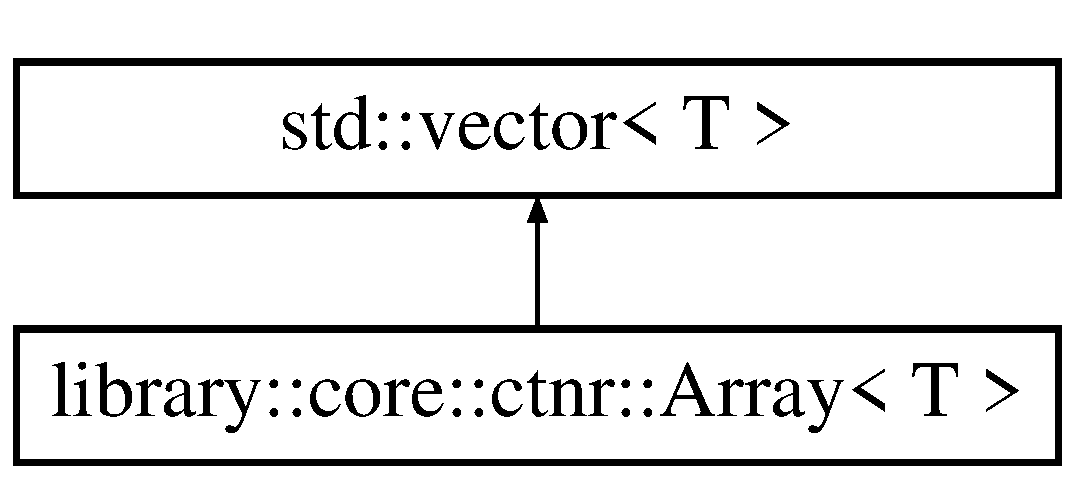
\includegraphics[height=2.000000cm]{classlibrary_1_1core_1_1ctnr_1_1_array}
\end{center}
\end{figure}
\subsection*{Public Types}
\begin{DoxyCompactItemize}
\item 
\mbox{\Hypertarget{classlibrary_1_1core_1_1ctnr_1_1_array_ac26454f2a2ad4013873386a70aa25fc4}\label{classlibrary_1_1core_1_1ctnr_1_1_array_ac26454f2a2ad4013873386a70aa25fc4}} 
typedef std\+::vector$<$ T $>$\+::const\+\_\+iterator {\bfseries Const\+Iterator}
\item 
\mbox{\Hypertarget{classlibrary_1_1core_1_1ctnr_1_1_array_a2364a34e7bc76d3661c3d89c4729a0e4}\label{classlibrary_1_1core_1_1ctnr_1_1_array_a2364a34e7bc76d3661c3d89c4729a0e4}} 
typedef std\+::vector$<$ T $>$\+::iterator {\bfseries Iterator}
\item 
\mbox{\Hypertarget{classlibrary_1_1core_1_1ctnr_1_1_array_a74cd325a740870aea490b6b739aa06ae}\label{classlibrary_1_1core_1_1ctnr_1_1_array_a74cd325a740870aea490b6b739aa06ae}} 
typedef std\+::function$<$ bool(const T \&)$>$ {\bfseries Predicate}
\end{DoxyCompactItemize}
\subsection*{Public Member Functions}
\begin{DoxyCompactItemize}
\item 
\mbox{\Hypertarget{classlibrary_1_1core_1_1ctnr_1_1_array_a95de936b24bfdf0a5d24ef45df892ecf}\label{classlibrary_1_1core_1_1ctnr_1_1_array_a95de936b24bfdf0a5d24ef45df892ecf}} 
\hyperlink{classlibrary_1_1core_1_1ctnr_1_1_array_a95de936b24bfdf0a5d24ef45df892ecf}{Array} ()=delete
\begin{DoxyCompactList}\small\item\em Default constructor (disabled) \end{DoxyCompactList}\item 
\hyperlink{classlibrary_1_1core_1_1ctnr_1_1_array_a9b510b4e2a3f9d4a324dfd0feba01285}{Array} (const std\+::vector$<$ T $>$ \&a\+Vector)
\begin{DoxyCompactList}\small\item\em Constructs an array from a C++ Standard Library vector. \end{DoxyCompactList}\item 
\hyperlink{classlibrary_1_1core_1_1ctnr_1_1_array_a647190cec3e259a8d8ad173c18bf3020}{Array} (const Size \&a\+Size, const T \&a\+Value)
\begin{DoxyCompactList}\small\item\em Constructs an array of given size populated with a given value. \end{DoxyCompactList}\item 
\hyperlink{classlibrary_1_1core_1_1ctnr_1_1_array_adcda1d4d28575b580a978406107febbb}{Array} (std\+::initializer\+\_\+list$<$ T $>$ a\+List)
\begin{DoxyCompactList}\small\item\em Constructs an array using an initializer list. \end{DoxyCompactList}\item 
\hyperlink{classlibrary_1_1core_1_1ctnr_1_1_array}{Array}$<$ T $>$ \hyperlink{classlibrary_1_1core_1_1ctnr_1_1_array_a5d65732e2a07b268d9def2da3c955002}{operator+} (const \hyperlink{classlibrary_1_1core_1_1ctnr_1_1_array}{Array}$<$ T $>$ \&an\+Array) const
\begin{DoxyCompactList}\small\item\em Concatenate array. \end{DoxyCompactList}\item 
bool \hyperlink{classlibrary_1_1core_1_1ctnr_1_1_array_a77d943be46a6d0313be3f2c5ca66d231}{is\+Empty} () const
\begin{DoxyCompactList}\small\item\em Check if array is empty. \end{DoxyCompactList}\item 
bool \hyperlink{classlibrary_1_1core_1_1ctnr_1_1_array_a9c423eb8a34dddc81e0ede9435094e99}{contains} (const T \&an\+Element) const
\begin{DoxyCompactList}\small\item\em Check if array contains element (by value) \end{DoxyCompactList}\item 
const T \& \hyperlink{classlibrary_1_1core_1_1ctnr_1_1_array_afea012716d6cfffa2803606c0b244419}{access\+First} () const
\begin{DoxyCompactList}\small\item\em Access first element. \end{DoxyCompactList}\item 
const T \& \hyperlink{classlibrary_1_1core_1_1ctnr_1_1_array_ad95dcce8ddaf163903a2327f766dbc8a}{access\+Last} () const
\begin{DoxyCompactList}\small\item\em Access last element. \end{DoxyCompactList}\item 
Size \hyperlink{classlibrary_1_1core_1_1ctnr_1_1_array_a049307129c77f461b37ddca47edc7913}{get\+Size} () const
\begin{DoxyCompactList}\small\item\em Get array size. \end{DoxyCompactList}\item 
Index \hyperlink{classlibrary_1_1core_1_1ctnr_1_1_array_aa8a3e2745d72db8181b42e3cfb55415c}{get\+Index\+Of} (const T \&an\+Element) const
\begin{DoxyCompactList}\small\item\em Get index of element (by value) \end{DoxyCompactList}\item 
\hyperlink{classlibrary_1_1core_1_1types_1_1_string}{types\+::\+String} \hyperlink{classlibrary_1_1core_1_1ctnr_1_1_array_a6a3416cc26d2968239af631d946ba11b}{get\+String} () const
\begin{DoxyCompactList}\small\item\em Get string representation of array. \end{DoxyCompactList}\item 
\hyperlink{classlibrary_1_1core_1_1ctnr_1_1_array}{Array}$<$ const T $\ast$ $>$ \hyperlink{classlibrary_1_1core_1_1ctnr_1_1_array_a5359c59d344a6147c7c6ea1012411011}{access\+Where} (const \hyperlink{classlibrary_1_1core_1_1ctnr_1_1_array}{Array}$<$ T $>$\+::Predicate \&a\+Predicate) const
\begin{DoxyCompactList}\small\item\em Get array of pointers to element based on condition. \end{DoxyCompactList}\item 
\hyperlink{classlibrary_1_1core_1_1ctnr_1_1_array}{Array}$<$ T $>$ \hyperlink{classlibrary_1_1core_1_1ctnr_1_1_array_a62069b24d593b2265422cb8f3a149c44}{get\+Where} (const \hyperlink{classlibrary_1_1core_1_1ctnr_1_1_array}{Array}$<$ T $>$\+::Predicate \&a\+Predicate) const
\begin{DoxyCompactList}\small\item\em Get array of elements based on condition. \end{DoxyCompactList}\item 
\hyperlink{classlibrary_1_1core_1_1ctnr_1_1_array}{Array}$<$ T $>$\+::Const\+Iterator \hyperlink{classlibrary_1_1core_1_1ctnr_1_1_array_aeb8ed38b67b6031e27c188d89bd5cbbf}{find} (const T \&an\+Element) const
\begin{DoxyCompactList}\small\item\em Get iterator to element, finding by by value. \end{DoxyCompactList}\item 
T \& \hyperlink{classlibrary_1_1core_1_1ctnr_1_1_array_abb2068e46720e8df057b5410ac8879d5}{access\+First} ()
\begin{DoxyCompactList}\small\item\em Access first element. \end{DoxyCompactList}\item 
T \& \hyperlink{classlibrary_1_1core_1_1ctnr_1_1_array_ad6ea47ab09dfeebd6de0878d3ad2de25}{access\+Last} ()
\begin{DoxyCompactList}\small\item\em Access last element. \end{DoxyCompactList}\item 
void \hyperlink{classlibrary_1_1core_1_1ctnr_1_1_array_a388497f6bda07f69d61aa60099b991a8}{add} (const T \&an\+Element)
\begin{DoxyCompactList}\small\item\em Add element to array. \end{DoxyCompactList}\item 
void \hyperlink{classlibrary_1_1core_1_1ctnr_1_1_array_a8e295703797d6e41dad7a45e4101a6db}{remove} (const T \&an\+Element)
\begin{DoxyCompactList}\small\item\em Remove element from array (by value) \end{DoxyCompactList}\item 
void \hyperlink{classlibrary_1_1core_1_1ctnr_1_1_array_a8dd701c76ba2659ee2e438cff70fa971}{add} (const \hyperlink{classlibrary_1_1core_1_1ctnr_1_1_array}{Array}$<$ T $>$ \&an\+Array)
\begin{DoxyCompactList}\small\item\em Add elements to array. \end{DoxyCompactList}\item 
void \hyperlink{classlibrary_1_1core_1_1ctnr_1_1_array_ab37ca6fc14eefd1336544e05ba1b4d0e}{remove} (const \hyperlink{classlibrary_1_1core_1_1ctnr_1_1_array}{Array}$<$ T $>$ \&an\+Array)
\begin{DoxyCompactList}\small\item\em Remove elements from array (by value) \end{DoxyCompactList}\item 
void \hyperlink{classlibrary_1_1core_1_1ctnr_1_1_array_abe72cec38e65761df3eaddcfa9b7a44a}{merge\+With} (const \hyperlink{classlibrary_1_1core_1_1ctnr_1_1_array}{Array}$<$ T $>$ \&an\+Array)
\begin{DoxyCompactList}\small\item\em Merge array with another array. \end{DoxyCompactList}\item 
void \hyperlink{classlibrary_1_1core_1_1ctnr_1_1_array_a322b1bfc3a93ea18bf68eb0cff69e6d3}{remove\+Where} (const \hyperlink{classlibrary_1_1core_1_1ctnr_1_1_array}{Array}$<$ T $>$\+::Predicate \&a\+Predicate)
\begin{DoxyCompactList}\small\item\em Remove elements based on condition. \end{DoxyCompactList}\item 
\hyperlink{classlibrary_1_1core_1_1ctnr_1_1_array}{Array}$<$ T $>$\+::Iterator \hyperlink{classlibrary_1_1core_1_1ctnr_1_1_array_afece85f642e3c623bac197e25ad2d4ec}{find} (const T \&an\+Element)
\begin{DoxyCompactList}\small\item\em Get iterator to element, finding by by value. \end{DoxyCompactList}\end{DoxyCompactItemize}
\subsection*{Static Public Member Functions}
\begin{DoxyCompactItemize}
\item 
static \hyperlink{classlibrary_1_1core_1_1ctnr_1_1_array}{Array}$<$ T $>$ \hyperlink{classlibrary_1_1core_1_1ctnr_1_1_array_a7795ee997ae6008cd0bc8db607315524}{Empty} ()
\begin{DoxyCompactList}\small\item\em Constructs an empty array. \end{DoxyCompactList}\end{DoxyCompactItemize}
\subsection*{Friends}
\begin{DoxyCompactItemize}
\item 
{\footnotesize template$<$class U $>$ }\\std\+::ostream \& \hyperlink{classlibrary_1_1core_1_1ctnr_1_1_array_a9daa2d638e5bd693776f8bf6caae0802}{operator$<$$<$} (std\+::ostream \&an\+Output\+Stream, const \hyperlink{classlibrary_1_1core_1_1ctnr_1_1_array}{Array}$<$ U $>$ \&an\+Array)
\begin{DoxyCompactList}\small\item\em Output stream operator. \end{DoxyCompactList}\end{DoxyCompactItemize}


\subsection{Detailed Description}
\subsubsection*{template$<$class T$>$\newline
class library\+::core\+::ctnr\+::\+Array$<$ T $>$}

\hyperlink{classlibrary_1_1core_1_1ctnr_1_1_array}{Array} container. 

Sequence containers representing arrays that can change in size. Arrays use contiguous storage locations for their elements. 

\subsection{Constructor \& Destructor Documentation}
\mbox{\Hypertarget{classlibrary_1_1core_1_1ctnr_1_1_array_a9b510b4e2a3f9d4a324dfd0feba01285}\label{classlibrary_1_1core_1_1ctnr_1_1_array_a9b510b4e2a3f9d4a324dfd0feba01285}} 
\index{library\+::core\+::ctnr\+::\+Array@{library\+::core\+::ctnr\+::\+Array}!Array@{Array}}
\index{Array@{Array}!library\+::core\+::ctnr\+::\+Array@{library\+::core\+::ctnr\+::\+Array}}
\subsubsection{\texorpdfstring{Array()}{Array()}\hspace{0.1cm}{\footnotesize\ttfamily [1/3]}}
{\footnotesize\ttfamily template$<$class T$>$ \\
\hyperlink{classlibrary_1_1core_1_1ctnr_1_1_array}{library\+::core\+::ctnr\+::\+Array}$<$ T $>$\+::\hyperlink{classlibrary_1_1core_1_1ctnr_1_1_array}{Array} (\begin{DoxyParamCaption}\item[{const std\+::vector$<$ T $>$ \&}]{a\+Vector }\end{DoxyParamCaption})}



Constructs an array from a C++ Standard Library vector. 


\begin{DoxyCode}
std::vector<Integer> vector = \{1, 2, 3\} ;
Array<Integer> array(vector) ;
\end{DoxyCode}



\begin{DoxyParams}[1]{Parameters}
\mbox{\tt in}  & {\em a\+Vector} & A vector \\
\hline
\end{DoxyParams}
\mbox{\Hypertarget{classlibrary_1_1core_1_1ctnr_1_1_array_a647190cec3e259a8d8ad173c18bf3020}\label{classlibrary_1_1core_1_1ctnr_1_1_array_a647190cec3e259a8d8ad173c18bf3020}} 
\index{library\+::core\+::ctnr\+::\+Array@{library\+::core\+::ctnr\+::\+Array}!Array@{Array}}
\index{Array@{Array}!library\+::core\+::ctnr\+::\+Array@{library\+::core\+::ctnr\+::\+Array}}
\subsubsection{\texorpdfstring{Array()}{Array()}\hspace{0.1cm}{\footnotesize\ttfamily [2/3]}}
{\footnotesize\ttfamily template$<$class T$>$ \\
\hyperlink{classlibrary_1_1core_1_1ctnr_1_1_array}{library\+::core\+::ctnr\+::\+Array}$<$ T $>$\+::\hyperlink{classlibrary_1_1core_1_1ctnr_1_1_array}{Array} (\begin{DoxyParamCaption}\item[{const Size \&}]{a\+Size,  }\item[{const T \&}]{a\+Value }\end{DoxyParamCaption})}



Constructs an array of given size populated with a given value. 


\begin{DoxyCode}
Array<String> array(3, \textcolor{stringliteral}{"abc"}) ; \textcolor{comment}{// ["abc", "abc", "abc"]}
\end{DoxyCode}



\begin{DoxyParams}[1]{Parameters}
\mbox{\tt in}  & {\em a\+Size} & An array size \\
\hline
\mbox{\tt in}  & {\em a\+Value} & A value \\
\hline
\end{DoxyParams}
\mbox{\Hypertarget{classlibrary_1_1core_1_1ctnr_1_1_array_adcda1d4d28575b580a978406107febbb}\label{classlibrary_1_1core_1_1ctnr_1_1_array_adcda1d4d28575b580a978406107febbb}} 
\index{library\+::core\+::ctnr\+::\+Array@{library\+::core\+::ctnr\+::\+Array}!Array@{Array}}
\index{Array@{Array}!library\+::core\+::ctnr\+::\+Array@{library\+::core\+::ctnr\+::\+Array}}
\subsubsection{\texorpdfstring{Array()}{Array()}\hspace{0.1cm}{\footnotesize\ttfamily [3/3]}}
{\footnotesize\ttfamily template$<$class T$>$ \\
\hyperlink{classlibrary_1_1core_1_1ctnr_1_1_array}{library\+::core\+::ctnr\+::\+Array}$<$ T $>$\+::\hyperlink{classlibrary_1_1core_1_1ctnr_1_1_array}{Array} (\begin{DoxyParamCaption}\item[{std\+::initializer\+\_\+list$<$ T $>$}]{a\+List }\end{DoxyParamCaption})}



Constructs an array using an initializer list. 


\begin{DoxyCode}
Array<Integer> array = \{1, 2, 3\} ;
\end{DoxyCode}



\begin{DoxyParams}[1]{Parameters}
\mbox{\tt in}  & {\em a\+List} & An initializer list \\
\hline
\end{DoxyParams}


\subsection{Member Function Documentation}
\mbox{\Hypertarget{classlibrary_1_1core_1_1ctnr_1_1_array_afea012716d6cfffa2803606c0b244419}\label{classlibrary_1_1core_1_1ctnr_1_1_array_afea012716d6cfffa2803606c0b244419}} 
\index{library\+::core\+::ctnr\+::\+Array@{library\+::core\+::ctnr\+::\+Array}!access\+First@{access\+First}}
\index{access\+First@{access\+First}!library\+::core\+::ctnr\+::\+Array@{library\+::core\+::ctnr\+::\+Array}}
\subsubsection{\texorpdfstring{access\+First()}{accessFirst()}\hspace{0.1cm}{\footnotesize\ttfamily [1/2]}}
{\footnotesize\ttfamily template$<$class T$>$ \\
const T\& \hyperlink{classlibrary_1_1core_1_1ctnr_1_1_array}{library\+::core\+::ctnr\+::\+Array}$<$ T $>$\+::access\+First (\begin{DoxyParamCaption}{ }\end{DoxyParamCaption}) const}



Access first element. 


\begin{DoxyCode}
Array<Integer> array = \{1, 2, 3\} ;
\textcolor{keyword}{const} Integer& element = array.accessFirst() ; \textcolor{comment}{// 1}
\end{DoxyCode}


\begin{DoxyReturn}{Returns}
Reference to the first element of array 
\end{DoxyReturn}
\mbox{\Hypertarget{classlibrary_1_1core_1_1ctnr_1_1_array_abb2068e46720e8df057b5410ac8879d5}\label{classlibrary_1_1core_1_1ctnr_1_1_array_abb2068e46720e8df057b5410ac8879d5}} 
\index{library\+::core\+::ctnr\+::\+Array@{library\+::core\+::ctnr\+::\+Array}!access\+First@{access\+First}}
\index{access\+First@{access\+First}!library\+::core\+::ctnr\+::\+Array@{library\+::core\+::ctnr\+::\+Array}}
\subsubsection{\texorpdfstring{access\+First()}{accessFirst()}\hspace{0.1cm}{\footnotesize\ttfamily [2/2]}}
{\footnotesize\ttfamily template$<$class T$>$ \\
T\& \hyperlink{classlibrary_1_1core_1_1ctnr_1_1_array}{library\+::core\+::ctnr\+::\+Array}$<$ T $>$\+::access\+First (\begin{DoxyParamCaption}{ }\end{DoxyParamCaption})}



Access first element. 


\begin{DoxyCode}
Array<Integer> array = \{1, 2, 3\} ;
Integer& element = array.accessFirst() ; \textcolor{comment}{// 1}
\end{DoxyCode}


\begin{DoxyReturn}{Returns}
Reference to the first element of array 
\end{DoxyReturn}
\mbox{\Hypertarget{classlibrary_1_1core_1_1ctnr_1_1_array_ad95dcce8ddaf163903a2327f766dbc8a}\label{classlibrary_1_1core_1_1ctnr_1_1_array_ad95dcce8ddaf163903a2327f766dbc8a}} 
\index{library\+::core\+::ctnr\+::\+Array@{library\+::core\+::ctnr\+::\+Array}!access\+Last@{access\+Last}}
\index{access\+Last@{access\+Last}!library\+::core\+::ctnr\+::\+Array@{library\+::core\+::ctnr\+::\+Array}}
\subsubsection{\texorpdfstring{access\+Last()}{accessLast()}\hspace{0.1cm}{\footnotesize\ttfamily [1/2]}}
{\footnotesize\ttfamily template$<$class T$>$ \\
const T\& \hyperlink{classlibrary_1_1core_1_1ctnr_1_1_array}{library\+::core\+::ctnr\+::\+Array}$<$ T $>$\+::access\+Last (\begin{DoxyParamCaption}{ }\end{DoxyParamCaption}) const}



Access last element. 


\begin{DoxyCode}
Array<Integer> array = \{1, 2, 3\} ;
\textcolor{keyword}{const} Integer& element = array.accessLast() ; \textcolor{comment}{// 3}
\end{DoxyCode}


\begin{DoxyReturn}{Returns}
Reference to the last element of array 
\end{DoxyReturn}
\mbox{\Hypertarget{classlibrary_1_1core_1_1ctnr_1_1_array_ad6ea47ab09dfeebd6de0878d3ad2de25}\label{classlibrary_1_1core_1_1ctnr_1_1_array_ad6ea47ab09dfeebd6de0878d3ad2de25}} 
\index{library\+::core\+::ctnr\+::\+Array@{library\+::core\+::ctnr\+::\+Array}!access\+Last@{access\+Last}}
\index{access\+Last@{access\+Last}!library\+::core\+::ctnr\+::\+Array@{library\+::core\+::ctnr\+::\+Array}}
\subsubsection{\texorpdfstring{access\+Last()}{accessLast()}\hspace{0.1cm}{\footnotesize\ttfamily [2/2]}}
{\footnotesize\ttfamily template$<$class T$>$ \\
T\& \hyperlink{classlibrary_1_1core_1_1ctnr_1_1_array}{library\+::core\+::ctnr\+::\+Array}$<$ T $>$\+::access\+Last (\begin{DoxyParamCaption}{ }\end{DoxyParamCaption})}



Access last element. 


\begin{DoxyCode}
Array<Integer> array = \{1, 2, 3\} ;
Integer& element = array.accessLast() ; \textcolor{comment}{// 3}
\end{DoxyCode}


\begin{DoxyReturn}{Returns}
Reference to the last element of array 
\end{DoxyReturn}
\mbox{\Hypertarget{classlibrary_1_1core_1_1ctnr_1_1_array_a5359c59d344a6147c7c6ea1012411011}\label{classlibrary_1_1core_1_1ctnr_1_1_array_a5359c59d344a6147c7c6ea1012411011}} 
\index{library\+::core\+::ctnr\+::\+Array@{library\+::core\+::ctnr\+::\+Array}!access\+Where@{access\+Where}}
\index{access\+Where@{access\+Where}!library\+::core\+::ctnr\+::\+Array@{library\+::core\+::ctnr\+::\+Array}}
\subsubsection{\texorpdfstring{access\+Where()}{accessWhere()}}
{\footnotesize\ttfamily template$<$class T$>$ \\
\hyperlink{classlibrary_1_1core_1_1ctnr_1_1_array}{Array}$<$const T$\ast$$>$ \hyperlink{classlibrary_1_1core_1_1ctnr_1_1_array}{library\+::core\+::ctnr\+::\+Array}$<$ T $>$\+::access\+Where (\begin{DoxyParamCaption}\item[{const \hyperlink{classlibrary_1_1core_1_1ctnr_1_1_array}{Array}$<$ T $>$\+::Predicate \&}]{a\+Predicate }\end{DoxyParamCaption}) const}



Get array of pointers to element based on condition. 


\begin{DoxyCode}
Array<Integer> array = \{0, 1, 2, 3, 4\} ;
Array<const Integer*> elements = array.accessWhere([] (\textcolor{keyword}{const} Integer& anInteger) -> \textcolor{keywordtype}{bool} \{ \textcolor{keywordflow}{return} anInteger
      .isEven() ; \}) ; \textcolor{comment}{// [&0, &2, &4]}
\end{DoxyCode}



\begin{DoxyParams}[1]{Parameters}
\mbox{\tt in}  & {\em a\+Predicate} & A predicate \\
\hline
\end{DoxyParams}
\begin{DoxyReturn}{Returns}
\hyperlink{classlibrary_1_1core_1_1ctnr_1_1_array}{Array} of pointers to element 
\end{DoxyReturn}
\mbox{\Hypertarget{classlibrary_1_1core_1_1ctnr_1_1_array_a388497f6bda07f69d61aa60099b991a8}\label{classlibrary_1_1core_1_1ctnr_1_1_array_a388497f6bda07f69d61aa60099b991a8}} 
\index{library\+::core\+::ctnr\+::\+Array@{library\+::core\+::ctnr\+::\+Array}!add@{add}}
\index{add@{add}!library\+::core\+::ctnr\+::\+Array@{library\+::core\+::ctnr\+::\+Array}}
\subsubsection{\texorpdfstring{add()}{add()}\hspace{0.1cm}{\footnotesize\ttfamily [1/2]}}
{\footnotesize\ttfamily template$<$class T$>$ \\
void \hyperlink{classlibrary_1_1core_1_1ctnr_1_1_array}{library\+::core\+::ctnr\+::\+Array}$<$ T $>$\+::add (\begin{DoxyParamCaption}\item[{const T \&}]{an\+Element }\end{DoxyParamCaption})}



Add element to array. 


\begin{DoxyCode}
Array<Integer> array = \{1, 2, 3\} ;
array.add(4) ; \textcolor{comment}{// [1, 2, 3, 4]}
\end{DoxyCode}



\begin{DoxyParams}[1]{Parameters}
\mbox{\tt in}  & {\em an\+Element} & An element \\
\hline
\end{DoxyParams}
\mbox{\Hypertarget{classlibrary_1_1core_1_1ctnr_1_1_array_a8dd701c76ba2659ee2e438cff70fa971}\label{classlibrary_1_1core_1_1ctnr_1_1_array_a8dd701c76ba2659ee2e438cff70fa971}} 
\index{library\+::core\+::ctnr\+::\+Array@{library\+::core\+::ctnr\+::\+Array}!add@{add}}
\index{add@{add}!library\+::core\+::ctnr\+::\+Array@{library\+::core\+::ctnr\+::\+Array}}
\subsubsection{\texorpdfstring{add()}{add()}\hspace{0.1cm}{\footnotesize\ttfamily [2/2]}}
{\footnotesize\ttfamily template$<$class T$>$ \\
void \hyperlink{classlibrary_1_1core_1_1ctnr_1_1_array}{library\+::core\+::ctnr\+::\+Array}$<$ T $>$\+::add (\begin{DoxyParamCaption}\item[{const \hyperlink{classlibrary_1_1core_1_1ctnr_1_1_array}{Array}$<$ T $>$ \&}]{an\+Array }\end{DoxyParamCaption})}



Add elements to array. 


\begin{DoxyCode}
Array<Integer> array = \{1, 2, 3\} ;
array.add(\{4, 5\}) ; \textcolor{comment}{// [1, 2, 3, 4, 5]}
\end{DoxyCode}



\begin{DoxyParams}[1]{Parameters}
\mbox{\tt in}  & {\em an\+Array} & An array of elements \\
\hline
\end{DoxyParams}
\mbox{\Hypertarget{classlibrary_1_1core_1_1ctnr_1_1_array_a9c423eb8a34dddc81e0ede9435094e99}\label{classlibrary_1_1core_1_1ctnr_1_1_array_a9c423eb8a34dddc81e0ede9435094e99}} 
\index{library\+::core\+::ctnr\+::\+Array@{library\+::core\+::ctnr\+::\+Array}!contains@{contains}}
\index{contains@{contains}!library\+::core\+::ctnr\+::\+Array@{library\+::core\+::ctnr\+::\+Array}}
\subsubsection{\texorpdfstring{contains()}{contains()}}
{\footnotesize\ttfamily template$<$class T$>$ \\
bool \hyperlink{classlibrary_1_1core_1_1ctnr_1_1_array}{library\+::core\+::ctnr\+::\+Array}$<$ T $>$\+::contains (\begin{DoxyParamCaption}\item[{const T \&}]{an\+Element }\end{DoxyParamCaption}) const}



Check if array contains element (by value) 


\begin{DoxyCode}
Array<Integer> array = \{1, 2, 3\} ;
array.contains(2) ; \textcolor{comment}{// True}
\end{DoxyCode}



\begin{DoxyParams}[1]{Parameters}
\mbox{\tt in}  & {\em an\+Element} & An element \\
\hline
\end{DoxyParams}
\begin{DoxyReturn}{Returns}
True if array contains element (by value) 
\end{DoxyReturn}
\mbox{\Hypertarget{classlibrary_1_1core_1_1ctnr_1_1_array_a7795ee997ae6008cd0bc8db607315524}\label{classlibrary_1_1core_1_1ctnr_1_1_array_a7795ee997ae6008cd0bc8db607315524}} 
\index{library\+::core\+::ctnr\+::\+Array@{library\+::core\+::ctnr\+::\+Array}!Empty@{Empty}}
\index{Empty@{Empty}!library\+::core\+::ctnr\+::\+Array@{library\+::core\+::ctnr\+::\+Array}}
\subsubsection{\texorpdfstring{Empty()}{Empty()}}
{\footnotesize\ttfamily template$<$class T$>$ \\
static \hyperlink{classlibrary_1_1core_1_1ctnr_1_1_array}{Array}$<$T$>$ \hyperlink{classlibrary_1_1core_1_1ctnr_1_1_array}{library\+::core\+::ctnr\+::\+Array}$<$ T $>$\+::Empty (\begin{DoxyParamCaption}{ }\end{DoxyParamCaption})\hspace{0.3cm}{\ttfamily [static]}}



Constructs an empty array. 


\begin{DoxyCode}
Array<Integer> array = \hyperlink{classlibrary_1_1core_1_1ctnr_1_1_array_a7795ee997ae6008cd0bc8db607315524}{Array<Integer>::Empty}() ;
\end{DoxyCode}


\begin{DoxyReturn}{Returns}
Empty array 
\end{DoxyReturn}
\mbox{\Hypertarget{classlibrary_1_1core_1_1ctnr_1_1_array_aeb8ed38b67b6031e27c188d89bd5cbbf}\label{classlibrary_1_1core_1_1ctnr_1_1_array_aeb8ed38b67b6031e27c188d89bd5cbbf}} 
\index{library\+::core\+::ctnr\+::\+Array@{library\+::core\+::ctnr\+::\+Array}!find@{find}}
\index{find@{find}!library\+::core\+::ctnr\+::\+Array@{library\+::core\+::ctnr\+::\+Array}}
\subsubsection{\texorpdfstring{find()}{find()}\hspace{0.1cm}{\footnotesize\ttfamily [1/2]}}
{\footnotesize\ttfamily template$<$class T$>$ \\
\hyperlink{classlibrary_1_1core_1_1ctnr_1_1_array}{Array}$<$T$>$\+::Const\+Iterator \hyperlink{classlibrary_1_1core_1_1ctnr_1_1_array}{library\+::core\+::ctnr\+::\+Array}$<$ T $>$\+::find (\begin{DoxyParamCaption}\item[{const T \&}]{an\+Element }\end{DoxyParamCaption}) const}



Get iterator to element, finding by by value. 


\begin{DoxyCode}
Array<Integer> array = \{0, 1, 2, 3, 4\} ;
\textcolor{keyword}{auto} elementIt = array.find(2) ;
\end{DoxyCode}



\begin{DoxyParams}[1]{Parameters}
\mbox{\tt in}  & {\em an\+Element} & An element \\
\hline
\end{DoxyParams}
\begin{DoxyReturn}{Returns}
Iterator to element 
\end{DoxyReturn}
\mbox{\Hypertarget{classlibrary_1_1core_1_1ctnr_1_1_array_afece85f642e3c623bac197e25ad2d4ec}\label{classlibrary_1_1core_1_1ctnr_1_1_array_afece85f642e3c623bac197e25ad2d4ec}} 
\index{library\+::core\+::ctnr\+::\+Array@{library\+::core\+::ctnr\+::\+Array}!find@{find}}
\index{find@{find}!library\+::core\+::ctnr\+::\+Array@{library\+::core\+::ctnr\+::\+Array}}
\subsubsection{\texorpdfstring{find()}{find()}\hspace{0.1cm}{\footnotesize\ttfamily [2/2]}}
{\footnotesize\ttfamily template$<$class T$>$ \\
\hyperlink{classlibrary_1_1core_1_1ctnr_1_1_array}{Array}$<$T$>$\+::Iterator \hyperlink{classlibrary_1_1core_1_1ctnr_1_1_array}{library\+::core\+::ctnr\+::\+Array}$<$ T $>$\+::find (\begin{DoxyParamCaption}\item[{const T \&}]{an\+Element }\end{DoxyParamCaption})}



Get iterator to element, finding by by value. 


\begin{DoxyCode}
Array<Integer> array = \{0, 1, 2, 3, 4\} ;
\textcolor{keyword}{auto} elementIt = array.find(2) ;
\end{DoxyCode}



\begin{DoxyParams}[1]{Parameters}
\mbox{\tt in}  & {\em an\+Element} & An element \\
\hline
\end{DoxyParams}
\begin{DoxyReturn}{Returns}
Iterator to element 
\end{DoxyReturn}
\mbox{\Hypertarget{classlibrary_1_1core_1_1ctnr_1_1_array_aa8a3e2745d72db8181b42e3cfb55415c}\label{classlibrary_1_1core_1_1ctnr_1_1_array_aa8a3e2745d72db8181b42e3cfb55415c}} 
\index{library\+::core\+::ctnr\+::\+Array@{library\+::core\+::ctnr\+::\+Array}!get\+Index\+Of@{get\+Index\+Of}}
\index{get\+Index\+Of@{get\+Index\+Of}!library\+::core\+::ctnr\+::\+Array@{library\+::core\+::ctnr\+::\+Array}}
\subsubsection{\texorpdfstring{get\+Index\+Of()}{getIndexOf()}}
{\footnotesize\ttfamily template$<$class T$>$ \\
Index \hyperlink{classlibrary_1_1core_1_1ctnr_1_1_array}{library\+::core\+::ctnr\+::\+Array}$<$ T $>$\+::get\+Index\+Of (\begin{DoxyParamCaption}\item[{const T \&}]{an\+Element }\end{DoxyParamCaption}) const}



Get index of element (by value) 


\begin{DoxyCode}
Array<Integer> array = \{1, 2, 3\} ;
\hyperlink{_index_8hpp_ad87eeb821d7067ec94e06ed1980d6350}{Index} index = array.getIndexOf(2) ; \textcolor{comment}{// 1}
\end{DoxyCode}



\begin{DoxyParams}[1]{Parameters}
\mbox{\tt in}  & {\em an\+Element} & An element \\
\hline
\end{DoxyParams}
\begin{DoxyReturn}{Returns}
Index of element (by value) 
\end{DoxyReturn}
\mbox{\Hypertarget{classlibrary_1_1core_1_1ctnr_1_1_array_a049307129c77f461b37ddca47edc7913}\label{classlibrary_1_1core_1_1ctnr_1_1_array_a049307129c77f461b37ddca47edc7913}} 
\index{library\+::core\+::ctnr\+::\+Array@{library\+::core\+::ctnr\+::\+Array}!get\+Size@{get\+Size}}
\index{get\+Size@{get\+Size}!library\+::core\+::ctnr\+::\+Array@{library\+::core\+::ctnr\+::\+Array}}
\subsubsection{\texorpdfstring{get\+Size()}{getSize()}}
{\footnotesize\ttfamily template$<$class T$>$ \\
Size \hyperlink{classlibrary_1_1core_1_1ctnr_1_1_array}{library\+::core\+::ctnr\+::\+Array}$<$ T $>$\+::get\+Size (\begin{DoxyParamCaption}{ }\end{DoxyParamCaption}) const}



Get array size. 


\begin{DoxyCode}
Array<Integer> array = \{1, 2, 3\} ;
\hyperlink{_size_8hpp_a701626ea1027888ebbb8cfd0ff7adab0}{Size} size = array.getSize() ; \textcolor{comment}{// 3}
\end{DoxyCode}


\begin{DoxyReturn}{Returns}
\hyperlink{classlibrary_1_1core_1_1ctnr_1_1_array}{Array} size 
\end{DoxyReturn}
\mbox{\Hypertarget{classlibrary_1_1core_1_1ctnr_1_1_array_a6a3416cc26d2968239af631d946ba11b}\label{classlibrary_1_1core_1_1ctnr_1_1_array_a6a3416cc26d2968239af631d946ba11b}} 
\index{library\+::core\+::ctnr\+::\+Array@{library\+::core\+::ctnr\+::\+Array}!get\+String@{get\+String}}
\index{get\+String@{get\+String}!library\+::core\+::ctnr\+::\+Array@{library\+::core\+::ctnr\+::\+Array}}
\subsubsection{\texorpdfstring{get\+String()}{getString()}}
{\footnotesize\ttfamily template$<$class T$>$ \\
\hyperlink{classlibrary_1_1core_1_1types_1_1_string}{types\+::\+String} \hyperlink{classlibrary_1_1core_1_1ctnr_1_1_array}{library\+::core\+::ctnr\+::\+Array}$<$ T $>$\+::get\+String (\begin{DoxyParamCaption}{ }\end{DoxyParamCaption}) const}



Get string representation of array. 


\begin{DoxyCode}
Array<Integer> array = \{1, 2, 3\} ;
String \textcolor{keywordtype}{string} = array.getString() ; \textcolor{comment}{// "[1, 2, 3]"}
\end{DoxyCode}


\begin{DoxyReturn}{Returns}
String representation of array 
\end{DoxyReturn}
\mbox{\Hypertarget{classlibrary_1_1core_1_1ctnr_1_1_array_a62069b24d593b2265422cb8f3a149c44}\label{classlibrary_1_1core_1_1ctnr_1_1_array_a62069b24d593b2265422cb8f3a149c44}} 
\index{library\+::core\+::ctnr\+::\+Array@{library\+::core\+::ctnr\+::\+Array}!get\+Where@{get\+Where}}
\index{get\+Where@{get\+Where}!library\+::core\+::ctnr\+::\+Array@{library\+::core\+::ctnr\+::\+Array}}
\subsubsection{\texorpdfstring{get\+Where()}{getWhere()}}
{\footnotesize\ttfamily template$<$class T$>$ \\
\hyperlink{classlibrary_1_1core_1_1ctnr_1_1_array}{Array}$<$T$>$ \hyperlink{classlibrary_1_1core_1_1ctnr_1_1_array}{library\+::core\+::ctnr\+::\+Array}$<$ T $>$\+::get\+Where (\begin{DoxyParamCaption}\item[{const \hyperlink{classlibrary_1_1core_1_1ctnr_1_1_array}{Array}$<$ T $>$\+::Predicate \&}]{a\+Predicate }\end{DoxyParamCaption}) const}



Get array of elements based on condition. 


\begin{DoxyCode}
Array<Integer> array = \{0, 1, 2, 3, 4\} ;
Array<const Integer*> elements = array.accessWhere([] (\textcolor{keyword}{const} Integer& anInteger) -> \textcolor{keywordtype}{bool} \{ \textcolor{keywordflow}{return} anInteger
      .isEven() ; \}) ; \textcolor{comment}{// [0, 2, 4]}
\end{DoxyCode}



\begin{DoxyParams}[1]{Parameters}
\mbox{\tt in}  & {\em a\+Predicate} & A predicate \\
\hline
\end{DoxyParams}
\begin{DoxyReturn}{Returns}
\hyperlink{classlibrary_1_1core_1_1ctnr_1_1_array}{Array} of elements 
\end{DoxyReturn}
\mbox{\Hypertarget{classlibrary_1_1core_1_1ctnr_1_1_array_a77d943be46a6d0313be3f2c5ca66d231}\label{classlibrary_1_1core_1_1ctnr_1_1_array_a77d943be46a6d0313be3f2c5ca66d231}} 
\index{library\+::core\+::ctnr\+::\+Array@{library\+::core\+::ctnr\+::\+Array}!is\+Empty@{is\+Empty}}
\index{is\+Empty@{is\+Empty}!library\+::core\+::ctnr\+::\+Array@{library\+::core\+::ctnr\+::\+Array}}
\subsubsection{\texorpdfstring{is\+Empty()}{isEmpty()}}
{\footnotesize\ttfamily template$<$class T$>$ \\
bool \hyperlink{classlibrary_1_1core_1_1ctnr_1_1_array}{library\+::core\+::ctnr\+::\+Array}$<$ T $>$\+::is\+Empty (\begin{DoxyParamCaption}{ }\end{DoxyParamCaption}) const}



Check if array is empty. 


\begin{DoxyCode}
Array<Integer> array = \{1, 2, 3\} ;
array.isEmpty() ; \textcolor{comment}{// False}
\end{DoxyCode}


\begin{DoxyReturn}{Returns}
True if array is empty 
\end{DoxyReturn}
\mbox{\Hypertarget{classlibrary_1_1core_1_1ctnr_1_1_array_abe72cec38e65761df3eaddcfa9b7a44a}\label{classlibrary_1_1core_1_1ctnr_1_1_array_abe72cec38e65761df3eaddcfa9b7a44a}} 
\index{library\+::core\+::ctnr\+::\+Array@{library\+::core\+::ctnr\+::\+Array}!merge\+With@{merge\+With}}
\index{merge\+With@{merge\+With}!library\+::core\+::ctnr\+::\+Array@{library\+::core\+::ctnr\+::\+Array}}
\subsubsection{\texorpdfstring{merge\+With()}{mergeWith()}}
{\footnotesize\ttfamily template$<$class T$>$ \\
void \hyperlink{classlibrary_1_1core_1_1ctnr_1_1_array}{library\+::core\+::ctnr\+::\+Array}$<$ T $>$\+::merge\+With (\begin{DoxyParamCaption}\item[{const \hyperlink{classlibrary_1_1core_1_1ctnr_1_1_array}{Array}$<$ T $>$ \&}]{an\+Array }\end{DoxyParamCaption})}



Merge array with another array. 


\begin{DoxyCode}
Array<Integer> firstArray = \{1, 2, 3\} ;
Array<Integer> secondArray = \{4, 5\} ;
firstArray.merge(secondArray) ; \textcolor{comment}{// [1, 2, 3, 4, 5]}
\end{DoxyCode}



\begin{DoxyParams}[1]{Parameters}
\mbox{\tt in}  & {\em an\+Array} & An array \\
\hline
\end{DoxyParams}
\mbox{\Hypertarget{classlibrary_1_1core_1_1ctnr_1_1_array_a5d65732e2a07b268d9def2da3c955002}\label{classlibrary_1_1core_1_1ctnr_1_1_array_a5d65732e2a07b268d9def2da3c955002}} 
\index{library\+::core\+::ctnr\+::\+Array@{library\+::core\+::ctnr\+::\+Array}!operator+@{operator+}}
\index{operator+@{operator+}!library\+::core\+::ctnr\+::\+Array@{library\+::core\+::ctnr\+::\+Array}}
\subsubsection{\texorpdfstring{operator+()}{operator+()}}
{\footnotesize\ttfamily template$<$class T$>$ \\
\hyperlink{classlibrary_1_1core_1_1ctnr_1_1_array}{Array}$<$T$>$ \hyperlink{classlibrary_1_1core_1_1ctnr_1_1_array}{library\+::core\+::ctnr\+::\+Array}$<$ T $>$\+::operator+ (\begin{DoxyParamCaption}\item[{const \hyperlink{classlibrary_1_1core_1_1ctnr_1_1_array}{Array}$<$ T $>$ \&}]{an\+Array }\end{DoxyParamCaption}) const}



Concatenate array. 


\begin{DoxyCode}
Array<Integer> a = \{1, 2, 3\} ;
Array<Integer> b = \{4, 5, 6\} ;
Array<Integer> c = a + b ; \textcolor{comment}{// \{1, 2, 3, 4, 5, 6\}}
\end{DoxyCode}



\begin{DoxyParams}[1]{Parameters}
\mbox{\tt in}  & {\em an\+Array} & An array to append \\
\hline
\end{DoxyParams}
\begin{DoxyReturn}{Returns}
An concatenated array 
\end{DoxyReturn}
\mbox{\Hypertarget{classlibrary_1_1core_1_1ctnr_1_1_array_a8e295703797d6e41dad7a45e4101a6db}\label{classlibrary_1_1core_1_1ctnr_1_1_array_a8e295703797d6e41dad7a45e4101a6db}} 
\index{library\+::core\+::ctnr\+::\+Array@{library\+::core\+::ctnr\+::\+Array}!remove@{remove}}
\index{remove@{remove}!library\+::core\+::ctnr\+::\+Array@{library\+::core\+::ctnr\+::\+Array}}
\subsubsection{\texorpdfstring{remove()}{remove()}\hspace{0.1cm}{\footnotesize\ttfamily [1/2]}}
{\footnotesize\ttfamily template$<$class T$>$ \\
void \hyperlink{classlibrary_1_1core_1_1ctnr_1_1_array}{library\+::core\+::ctnr\+::\+Array}$<$ T $>$\+::remove (\begin{DoxyParamCaption}\item[{const T \&}]{an\+Element }\end{DoxyParamCaption})}



Remove element from array (by value) 


\begin{DoxyCode}
Array<Integer> array = \{1, 2, 3\} ;
array.remove(2) ; \textcolor{comment}{// [1, 3]}
\end{DoxyCode}



\begin{DoxyParams}[1]{Parameters}
\mbox{\tt in}  & {\em an\+Element} & An element \\
\hline
\end{DoxyParams}
\mbox{\Hypertarget{classlibrary_1_1core_1_1ctnr_1_1_array_ab37ca6fc14eefd1336544e05ba1b4d0e}\label{classlibrary_1_1core_1_1ctnr_1_1_array_ab37ca6fc14eefd1336544e05ba1b4d0e}} 
\index{library\+::core\+::ctnr\+::\+Array@{library\+::core\+::ctnr\+::\+Array}!remove@{remove}}
\index{remove@{remove}!library\+::core\+::ctnr\+::\+Array@{library\+::core\+::ctnr\+::\+Array}}
\subsubsection{\texorpdfstring{remove()}{remove()}\hspace{0.1cm}{\footnotesize\ttfamily [2/2]}}
{\footnotesize\ttfamily template$<$class T$>$ \\
void \hyperlink{classlibrary_1_1core_1_1ctnr_1_1_array}{library\+::core\+::ctnr\+::\+Array}$<$ T $>$\+::remove (\begin{DoxyParamCaption}\item[{const \hyperlink{classlibrary_1_1core_1_1ctnr_1_1_array}{Array}$<$ T $>$ \&}]{an\+Array }\end{DoxyParamCaption})}



Remove elements from array (by value) 


\begin{DoxyCode}
Array<Integer> array = \{1, 2, 3, 4, 5\} ;
array.remove(\{2, 4\}) ; \textcolor{comment}{// [1, 3, 5]}
\end{DoxyCode}



\begin{DoxyParams}[1]{Parameters}
\mbox{\tt in}  & {\em an\+Array} & An array of elements \\
\hline
\end{DoxyParams}
\mbox{\Hypertarget{classlibrary_1_1core_1_1ctnr_1_1_array_a322b1bfc3a93ea18bf68eb0cff69e6d3}\label{classlibrary_1_1core_1_1ctnr_1_1_array_a322b1bfc3a93ea18bf68eb0cff69e6d3}} 
\index{library\+::core\+::ctnr\+::\+Array@{library\+::core\+::ctnr\+::\+Array}!remove\+Where@{remove\+Where}}
\index{remove\+Where@{remove\+Where}!library\+::core\+::ctnr\+::\+Array@{library\+::core\+::ctnr\+::\+Array}}
\subsubsection{\texorpdfstring{remove\+Where()}{removeWhere()}}
{\footnotesize\ttfamily template$<$class T$>$ \\
void \hyperlink{classlibrary_1_1core_1_1ctnr_1_1_array}{library\+::core\+::ctnr\+::\+Array}$<$ T $>$\+::remove\+Where (\begin{DoxyParamCaption}\item[{const \hyperlink{classlibrary_1_1core_1_1ctnr_1_1_array}{Array}$<$ T $>$\+::Predicate \&}]{a\+Predicate }\end{DoxyParamCaption})}



Remove elements based on condition. 


\begin{DoxyCode}
Array<Integer> array = \{1, 2, 3, 4, 5\} ;
array.removeWhere([] (\textcolor{keyword}{const} Integer& anInteger) -> \textcolor{keywordtype}{bool} \{ \textcolor{keywordflow}{return} anInteger.isEven() ; \}) ; \textcolor{comment}{// [1, 3, 5]}
\end{DoxyCode}



\begin{DoxyParams}[1]{Parameters}
\mbox{\tt in}  & {\em a\+Predicate} & A predicate \\
\hline
\end{DoxyParams}


\subsection{Friends And Related Function Documentation}
\mbox{\Hypertarget{classlibrary_1_1core_1_1ctnr_1_1_array_a9daa2d638e5bd693776f8bf6caae0802}\label{classlibrary_1_1core_1_1ctnr_1_1_array_a9daa2d638e5bd693776f8bf6caae0802}} 
\index{library\+::core\+::ctnr\+::\+Array@{library\+::core\+::ctnr\+::\+Array}!operator$<$$<$@{operator$<$$<$}}
\index{operator$<$$<$@{operator$<$$<$}!library\+::core\+::ctnr\+::\+Array@{library\+::core\+::ctnr\+::\+Array}}
\subsubsection{\texorpdfstring{operator$<$$<$}{operator<<}}
{\footnotesize\ttfamily template$<$class T$>$ \\
template$<$class U $>$ \\
std\+::ostream\& operator$<$$<$ (\begin{DoxyParamCaption}\item[{std\+::ostream \&}]{an\+Output\+Stream,  }\item[{const \hyperlink{classlibrary_1_1core_1_1ctnr_1_1_array}{Array}$<$ U $>$ \&}]{an\+Array }\end{DoxyParamCaption})\hspace{0.3cm}{\ttfamily [friend]}}



Output stream operator. 


\begin{DoxyCode}
Array<Integer> array = \{1, 2, 3\} ;
std::cout << array ;
\end{DoxyCode}



\begin{DoxyParams}[1]{Parameters}
\mbox{\tt in}  & {\em an\+Output\+Stream} & An output stream \\
\hline
\mbox{\tt in}  & {\em an\+Array} & An array \\
\hline
\end{DoxyParams}
\begin{DoxyReturn}{Returns}
An output stream 
\end{DoxyReturn}


The documentation for this class was generated from the following file\+:\begin{DoxyCompactItemize}
\item 
include/\+Library/\+Core/\+Containers/\hyperlink{_array_8hpp}{Array.\+hpp}\end{DoxyCompactItemize}

\hypertarget{classlibrary_1_1core_1_1types_1_1_byte_array}{}\section{library\+:\+:core\+:\+:types\+:\+:Byte\+Array Class Reference}
\label{classlibrary_1_1core_1_1types_1_1_byte_array}\index{library\+::core\+::types\+::\+Byte\+Array@{library\+::core\+::types\+::\+Byte\+Array}}


An array of bytes \mbox{[}T\+BI\mbox{]}.  




{\ttfamily \#include $<$Byte\+Array.\+hpp$>$}

\subsection*{Public Member Functions}
\begin{DoxyCompactItemize}
\item 
\hyperlink{classlibrary_1_1core_1_1types_1_1_byte_array_a68d34286659b8a03655990e98b794880}{Byte\+Array} ()=default
\end{DoxyCompactItemize}


\subsection{Detailed Description}
An array of bytes \mbox{[}T\+BI\mbox{]}. 

\subsection{Constructor \& Destructor Documentation}
\mbox{\Hypertarget{classlibrary_1_1core_1_1types_1_1_byte_array_a68d34286659b8a03655990e98b794880}\label{classlibrary_1_1core_1_1types_1_1_byte_array_a68d34286659b8a03655990e98b794880}} 
\index{library\+::core\+::types\+::\+Byte\+Array@{library\+::core\+::types\+::\+Byte\+Array}!Byte\+Array@{Byte\+Array}}
\index{Byte\+Array@{Byte\+Array}!library\+::core\+::types\+::\+Byte\+Array@{library\+::core\+::types\+::\+Byte\+Array}}
\subsubsection{\texorpdfstring{Byte\+Array()}{ByteArray()}}
{\footnotesize\ttfamily library\+::core\+::types\+::\+Byte\+Array\+::\+Byte\+Array (\begin{DoxyParamCaption}{ }\end{DoxyParamCaption})\hspace{0.3cm}{\ttfamily [default]}}



The documentation for this class was generated from the following file\+:\begin{DoxyCompactItemize}
\item 
include/\+Library/\+Core/\+Types/\hyperlink{_byte_array_8hpp}{Byte\+Array.\+hpp}\end{DoxyCompactItemize}

\hypertarget{classlibrary_1_1core_1_1logger_1_1sinks_1_1_console}{}\section{library\+:\+:core\+:\+:logger\+:\+:sinks\+:\+:Console Class Reference}
\label{classlibrary_1_1core_1_1logger_1_1sinks_1_1_console}\index{library\+::core\+::logger\+::sinks\+::\+Console@{library\+::core\+::logger\+::sinks\+::\+Console}}


Log console sink.  




{\ttfamily \#include $<$Console.\+hpp$>$}

Inheritance diagram for library\+:\+:core\+:\+:logger\+:\+:sinks\+:\+:Console\+:\begin{figure}[H]
\begin{center}
\leavevmode
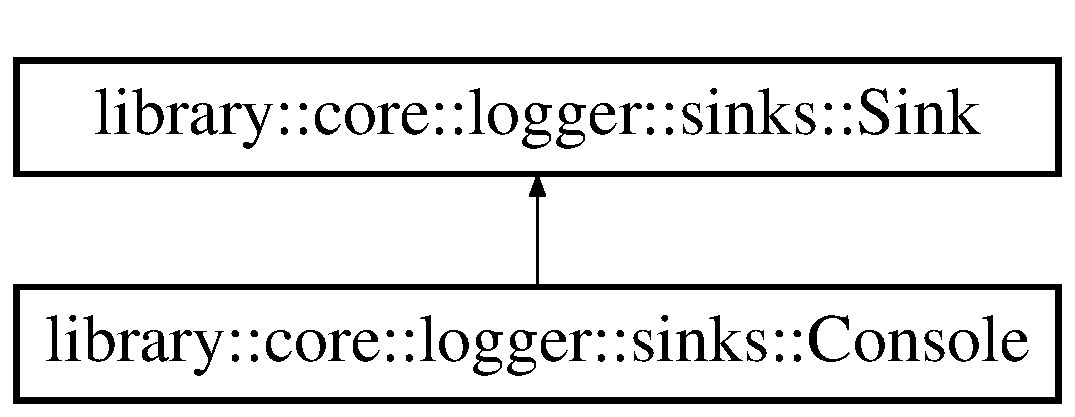
\includegraphics[height=2.000000cm]{classlibrary_1_1core_1_1logger_1_1sinks_1_1_console}
\end{center}
\end{figure}
\subsection*{Public Types}
\begin{DoxyCompactItemize}
\item 
enum \hyperlink{classlibrary_1_1core_1_1logger_1_1sinks_1_1_console_aa7a07d8165e1df74ad4d289d5220bc96}{Color} \{ \newline
\hyperlink{classlibrary_1_1core_1_1logger_1_1sinks_1_1_console_aa7a07d8165e1df74ad4d289d5220bc96ae90dfb84e30edf611e326eeb04d680de}{Color\+::\+Black}, 
\hyperlink{classlibrary_1_1core_1_1logger_1_1sinks_1_1_console_aa7a07d8165e1df74ad4d289d5220bc96aee38e4d5dd68c4e440825018d549cb47}{Color\+::\+Red}, 
\hyperlink{classlibrary_1_1core_1_1logger_1_1sinks_1_1_console_aa7a07d8165e1df74ad4d289d5220bc96ad382816a3cbeed082c9e216e7392eed1}{Color\+::\+Green}, 
\hyperlink{classlibrary_1_1core_1_1logger_1_1sinks_1_1_console_aa7a07d8165e1df74ad4d289d5220bc96a51e6cd92b6c45f9affdc158ecca2b8b8}{Color\+::\+Yellow}, 
\newline
\hyperlink{classlibrary_1_1core_1_1logger_1_1sinks_1_1_console_aa7a07d8165e1df74ad4d289d5220bc96a9594eec95be70e7b1710f730fdda33d9}{Color\+::\+Blue}, 
\hyperlink{classlibrary_1_1core_1_1logger_1_1sinks_1_1_console_aa7a07d8165e1df74ad4d289d5220bc96ab91cc2c1416fcca942b61c7ac5b1a9ac}{Color\+::\+Magenta}, 
\hyperlink{classlibrary_1_1core_1_1logger_1_1sinks_1_1_console_aa7a07d8165e1df74ad4d289d5220bc96a023c239d2f2538f140a20e72c7b73f20}{Color\+::\+Cyan}, 
\hyperlink{classlibrary_1_1core_1_1logger_1_1sinks_1_1_console_aa7a07d8165e1df74ad4d289d5220bc96afb55202637692de4a494e9ade4cff2dd}{Color\+::\+Light\+Gray}, 
\newline
\hyperlink{classlibrary_1_1core_1_1logger_1_1sinks_1_1_console_aa7a07d8165e1df74ad4d289d5220bc96a91e93fc984985226ad4d319a4e4134ab}{Color\+::\+Dark\+Gray}, 
\hyperlink{classlibrary_1_1core_1_1logger_1_1sinks_1_1_console_aa7a07d8165e1df74ad4d289d5220bc96af9a96fb667261a141d10021a66d6ad0f}{Color\+::\+Light\+Red}, 
\hyperlink{classlibrary_1_1core_1_1logger_1_1sinks_1_1_console_aa7a07d8165e1df74ad4d289d5220bc96a7a6a38bec67cbc2a39ce22f34e4ed8e2}{Color\+::\+Light\+Green}, 
\hyperlink{classlibrary_1_1core_1_1logger_1_1sinks_1_1_console_aa7a07d8165e1df74ad4d289d5220bc96afaf948b65bda38f44b17d156177d1728}{Color\+::\+Light\+Yellow}, 
\newline
\hyperlink{classlibrary_1_1core_1_1logger_1_1sinks_1_1_console_aa7a07d8165e1df74ad4d289d5220bc96a4d7ff7393a484a7b9ed2e381f5cdeaf7}{Color\+::\+Light\+Blue}, 
\hyperlink{classlibrary_1_1core_1_1logger_1_1sinks_1_1_console_aa7a07d8165e1df74ad4d289d5220bc96af1ec64ef9f82e9fb86b094f8b548f9f1}{Color\+::\+Light\+Magenta}, 
\hyperlink{classlibrary_1_1core_1_1logger_1_1sinks_1_1_console_aa7a07d8165e1df74ad4d289d5220bc96ac37b5ce4ba80a097d82726ae74d34b13}{Color\+::\+Light\+Cyan}, 
\hyperlink{classlibrary_1_1core_1_1logger_1_1sinks_1_1_console_aa7a07d8165e1df74ad4d289d5220bc96a25a81701fbfa4a1efdf660a950c1d006}{Color\+::\+White}
 \}
\end{DoxyCompactItemize}
\subsection*{Public Member Functions}
\begin{DoxyCompactItemize}
\item 
\hyperlink{classlibrary_1_1core_1_1logger_1_1sinks_1_1_console_a6baabd0bce6777b665aba8b30c40c0d8}{Console} (const \hyperlink{namespacelibrary_1_1core_1_1logger_a35f71353edf64f68f7fe3874b01abaa8}{Severity} \&a\+Severity)
\item 
\hyperlink{classlibrary_1_1core_1_1logger_1_1sinks_1_1_console_a6d7feabeb113b6448d0b83d114175328}{Console} (const \hyperlink{classlibrary_1_1core_1_1logger_1_1sinks_1_1_console}{Console} \&a\+Console)
\item 
virtual \hyperlink{classlibrary_1_1core_1_1logger_1_1sinks_1_1_console_adefb4276dd98ae3d6183b4c2351f88b6}{$\sim$\+Console} () override
\item 
virtual \hyperlink{classlibrary_1_1core_1_1logger_1_1sinks_1_1_console}{Console} $\ast$ \hyperlink{classlibrary_1_1core_1_1logger_1_1sinks_1_1_console_ac5c80193b0832f760a7447e7abc7d468}{clone} () const override
\item 
virtual void \hyperlink{classlibrary_1_1core_1_1logger_1_1sinks_1_1_console_a09190fa0b66fa9a03792e6a546590da9}{enable} () override
\item 
virtual void \hyperlink{classlibrary_1_1core_1_1logger_1_1sinks_1_1_console_adc1a648433f26cc4397f1e703c9506c7}{disable} () override
\end{DoxyCompactItemize}
\subsection*{Static Public Member Functions}
\begin{DoxyCompactItemize}
\item 
static \hyperlink{classlibrary_1_1core_1_1types_1_1_string}{String} \hyperlink{classlibrary_1_1core_1_1logger_1_1sinks_1_1_console_a9cf21ce963c2079b613bfb5788bb5659}{Colorize\+Message} (const \hyperlink{classlibrary_1_1core_1_1types_1_1_string}{String} \&a\+Message, const \hyperlink{classlibrary_1_1core_1_1logger_1_1sinks_1_1_console_aa7a07d8165e1df74ad4d289d5220bc96}{Console\+::\+Color} \&a\+Color)
\end{DoxyCompactItemize}
\subsection*{Friends}
\begin{DoxyCompactItemize}
\item 
class \hyperlink{classlibrary_1_1core_1_1logger_1_1sinks_1_1_console_aeda242f6bb74cf8f4003eb67666e9118}{Console\+::\+Impl}
\end{DoxyCompactItemize}
\subsection*{Additional Inherited Members}


\subsection{Detailed Description}
Log console sink. 

\subsection{Member Enumeration Documentation}
\mbox{\Hypertarget{classlibrary_1_1core_1_1logger_1_1sinks_1_1_console_aa7a07d8165e1df74ad4d289d5220bc96}\label{classlibrary_1_1core_1_1logger_1_1sinks_1_1_console_aa7a07d8165e1df74ad4d289d5220bc96}} 
\index{library\+::core\+::logger\+::sinks\+::\+Console@{library\+::core\+::logger\+::sinks\+::\+Console}!Color@{Color}}
\index{Color@{Color}!library\+::core\+::logger\+::sinks\+::\+Console@{library\+::core\+::logger\+::sinks\+::\+Console}}
\subsubsection{\texorpdfstring{Color}{Color}}
{\footnotesize\ttfamily enum \hyperlink{classlibrary_1_1core_1_1logger_1_1sinks_1_1_console_aa7a07d8165e1df74ad4d289d5220bc96}{library\+::core\+::logger\+::sinks\+::\+Console\+::\+Color}\hspace{0.3cm}{\ttfamily [strong]}}

\begin{DoxyEnumFields}{Enumerator}
\raisebox{\heightof{T}}[0pt][0pt]{\index{Black@{Black}!library\+::core\+::logger\+::sinks\+::\+Console@{library\+::core\+::logger\+::sinks\+::\+Console}}\index{library\+::core\+::logger\+::sinks\+::\+Console@{library\+::core\+::logger\+::sinks\+::\+Console}!Black@{Black}}}\mbox{\Hypertarget{classlibrary_1_1core_1_1logger_1_1sinks_1_1_console_aa7a07d8165e1df74ad4d289d5220bc96ae90dfb84e30edf611e326eeb04d680de}\label{classlibrary_1_1core_1_1logger_1_1sinks_1_1_console_aa7a07d8165e1df74ad4d289d5220bc96ae90dfb84e30edf611e326eeb04d680de}} 
Black&\\
\hline

\raisebox{\heightof{T}}[0pt][0pt]{\index{Red@{Red}!library\+::core\+::logger\+::sinks\+::\+Console@{library\+::core\+::logger\+::sinks\+::\+Console}}\index{library\+::core\+::logger\+::sinks\+::\+Console@{library\+::core\+::logger\+::sinks\+::\+Console}!Red@{Red}}}\mbox{\Hypertarget{classlibrary_1_1core_1_1logger_1_1sinks_1_1_console_aa7a07d8165e1df74ad4d289d5220bc96aee38e4d5dd68c4e440825018d549cb47}\label{classlibrary_1_1core_1_1logger_1_1sinks_1_1_console_aa7a07d8165e1df74ad4d289d5220bc96aee38e4d5dd68c4e440825018d549cb47}} 
Red&\\
\hline

\raisebox{\heightof{T}}[0pt][0pt]{\index{Green@{Green}!library\+::core\+::logger\+::sinks\+::\+Console@{library\+::core\+::logger\+::sinks\+::\+Console}}\index{library\+::core\+::logger\+::sinks\+::\+Console@{library\+::core\+::logger\+::sinks\+::\+Console}!Green@{Green}}}\mbox{\Hypertarget{classlibrary_1_1core_1_1logger_1_1sinks_1_1_console_aa7a07d8165e1df74ad4d289d5220bc96ad382816a3cbeed082c9e216e7392eed1}\label{classlibrary_1_1core_1_1logger_1_1sinks_1_1_console_aa7a07d8165e1df74ad4d289d5220bc96ad382816a3cbeed082c9e216e7392eed1}} 
Green&\\
\hline

\raisebox{\heightof{T}}[0pt][0pt]{\index{Yellow@{Yellow}!library\+::core\+::logger\+::sinks\+::\+Console@{library\+::core\+::logger\+::sinks\+::\+Console}}\index{library\+::core\+::logger\+::sinks\+::\+Console@{library\+::core\+::logger\+::sinks\+::\+Console}!Yellow@{Yellow}}}\mbox{\Hypertarget{classlibrary_1_1core_1_1logger_1_1sinks_1_1_console_aa7a07d8165e1df74ad4d289d5220bc96a51e6cd92b6c45f9affdc158ecca2b8b8}\label{classlibrary_1_1core_1_1logger_1_1sinks_1_1_console_aa7a07d8165e1df74ad4d289d5220bc96a51e6cd92b6c45f9affdc158ecca2b8b8}} 
Yellow&\\
\hline

\raisebox{\heightof{T}}[0pt][0pt]{\index{Blue@{Blue}!library\+::core\+::logger\+::sinks\+::\+Console@{library\+::core\+::logger\+::sinks\+::\+Console}}\index{library\+::core\+::logger\+::sinks\+::\+Console@{library\+::core\+::logger\+::sinks\+::\+Console}!Blue@{Blue}}}\mbox{\Hypertarget{classlibrary_1_1core_1_1logger_1_1sinks_1_1_console_aa7a07d8165e1df74ad4d289d5220bc96a9594eec95be70e7b1710f730fdda33d9}\label{classlibrary_1_1core_1_1logger_1_1sinks_1_1_console_aa7a07d8165e1df74ad4d289d5220bc96a9594eec95be70e7b1710f730fdda33d9}} 
Blue&\\
\hline

\raisebox{\heightof{T}}[0pt][0pt]{\index{Magenta@{Magenta}!library\+::core\+::logger\+::sinks\+::\+Console@{library\+::core\+::logger\+::sinks\+::\+Console}}\index{library\+::core\+::logger\+::sinks\+::\+Console@{library\+::core\+::logger\+::sinks\+::\+Console}!Magenta@{Magenta}}}\mbox{\Hypertarget{classlibrary_1_1core_1_1logger_1_1sinks_1_1_console_aa7a07d8165e1df74ad4d289d5220bc96ab91cc2c1416fcca942b61c7ac5b1a9ac}\label{classlibrary_1_1core_1_1logger_1_1sinks_1_1_console_aa7a07d8165e1df74ad4d289d5220bc96ab91cc2c1416fcca942b61c7ac5b1a9ac}} 
Magenta&\\
\hline

\raisebox{\heightof{T}}[0pt][0pt]{\index{Cyan@{Cyan}!library\+::core\+::logger\+::sinks\+::\+Console@{library\+::core\+::logger\+::sinks\+::\+Console}}\index{library\+::core\+::logger\+::sinks\+::\+Console@{library\+::core\+::logger\+::sinks\+::\+Console}!Cyan@{Cyan}}}\mbox{\Hypertarget{classlibrary_1_1core_1_1logger_1_1sinks_1_1_console_aa7a07d8165e1df74ad4d289d5220bc96a023c239d2f2538f140a20e72c7b73f20}\label{classlibrary_1_1core_1_1logger_1_1sinks_1_1_console_aa7a07d8165e1df74ad4d289d5220bc96a023c239d2f2538f140a20e72c7b73f20}} 
Cyan&\\
\hline

\raisebox{\heightof{T}}[0pt][0pt]{\index{Light\+Gray@{Light\+Gray}!library\+::core\+::logger\+::sinks\+::\+Console@{library\+::core\+::logger\+::sinks\+::\+Console}}\index{library\+::core\+::logger\+::sinks\+::\+Console@{library\+::core\+::logger\+::sinks\+::\+Console}!Light\+Gray@{Light\+Gray}}}\mbox{\Hypertarget{classlibrary_1_1core_1_1logger_1_1sinks_1_1_console_aa7a07d8165e1df74ad4d289d5220bc96afb55202637692de4a494e9ade4cff2dd}\label{classlibrary_1_1core_1_1logger_1_1sinks_1_1_console_aa7a07d8165e1df74ad4d289d5220bc96afb55202637692de4a494e9ade4cff2dd}} 
Light\+Gray&\\
\hline

\raisebox{\heightof{T}}[0pt][0pt]{\index{Dark\+Gray@{Dark\+Gray}!library\+::core\+::logger\+::sinks\+::\+Console@{library\+::core\+::logger\+::sinks\+::\+Console}}\index{library\+::core\+::logger\+::sinks\+::\+Console@{library\+::core\+::logger\+::sinks\+::\+Console}!Dark\+Gray@{Dark\+Gray}}}\mbox{\Hypertarget{classlibrary_1_1core_1_1logger_1_1sinks_1_1_console_aa7a07d8165e1df74ad4d289d5220bc96a91e93fc984985226ad4d319a4e4134ab}\label{classlibrary_1_1core_1_1logger_1_1sinks_1_1_console_aa7a07d8165e1df74ad4d289d5220bc96a91e93fc984985226ad4d319a4e4134ab}} 
Dark\+Gray&\\
\hline

\raisebox{\heightof{T}}[0pt][0pt]{\index{Light\+Red@{Light\+Red}!library\+::core\+::logger\+::sinks\+::\+Console@{library\+::core\+::logger\+::sinks\+::\+Console}}\index{library\+::core\+::logger\+::sinks\+::\+Console@{library\+::core\+::logger\+::sinks\+::\+Console}!Light\+Red@{Light\+Red}}}\mbox{\Hypertarget{classlibrary_1_1core_1_1logger_1_1sinks_1_1_console_aa7a07d8165e1df74ad4d289d5220bc96af9a96fb667261a141d10021a66d6ad0f}\label{classlibrary_1_1core_1_1logger_1_1sinks_1_1_console_aa7a07d8165e1df74ad4d289d5220bc96af9a96fb667261a141d10021a66d6ad0f}} 
Light\+Red&\\
\hline

\raisebox{\heightof{T}}[0pt][0pt]{\index{Light\+Green@{Light\+Green}!library\+::core\+::logger\+::sinks\+::\+Console@{library\+::core\+::logger\+::sinks\+::\+Console}}\index{library\+::core\+::logger\+::sinks\+::\+Console@{library\+::core\+::logger\+::sinks\+::\+Console}!Light\+Green@{Light\+Green}}}\mbox{\Hypertarget{classlibrary_1_1core_1_1logger_1_1sinks_1_1_console_aa7a07d8165e1df74ad4d289d5220bc96a7a6a38bec67cbc2a39ce22f34e4ed8e2}\label{classlibrary_1_1core_1_1logger_1_1sinks_1_1_console_aa7a07d8165e1df74ad4d289d5220bc96a7a6a38bec67cbc2a39ce22f34e4ed8e2}} 
Light\+Green&\\
\hline

\raisebox{\heightof{T}}[0pt][0pt]{\index{Light\+Yellow@{Light\+Yellow}!library\+::core\+::logger\+::sinks\+::\+Console@{library\+::core\+::logger\+::sinks\+::\+Console}}\index{library\+::core\+::logger\+::sinks\+::\+Console@{library\+::core\+::logger\+::sinks\+::\+Console}!Light\+Yellow@{Light\+Yellow}}}\mbox{\Hypertarget{classlibrary_1_1core_1_1logger_1_1sinks_1_1_console_aa7a07d8165e1df74ad4d289d5220bc96afaf948b65bda38f44b17d156177d1728}\label{classlibrary_1_1core_1_1logger_1_1sinks_1_1_console_aa7a07d8165e1df74ad4d289d5220bc96afaf948b65bda38f44b17d156177d1728}} 
Light\+Yellow&\\
\hline

\raisebox{\heightof{T}}[0pt][0pt]{\index{Light\+Blue@{Light\+Blue}!library\+::core\+::logger\+::sinks\+::\+Console@{library\+::core\+::logger\+::sinks\+::\+Console}}\index{library\+::core\+::logger\+::sinks\+::\+Console@{library\+::core\+::logger\+::sinks\+::\+Console}!Light\+Blue@{Light\+Blue}}}\mbox{\Hypertarget{classlibrary_1_1core_1_1logger_1_1sinks_1_1_console_aa7a07d8165e1df74ad4d289d5220bc96a4d7ff7393a484a7b9ed2e381f5cdeaf7}\label{classlibrary_1_1core_1_1logger_1_1sinks_1_1_console_aa7a07d8165e1df74ad4d289d5220bc96a4d7ff7393a484a7b9ed2e381f5cdeaf7}} 
Light\+Blue&\\
\hline

\raisebox{\heightof{T}}[0pt][0pt]{\index{Light\+Magenta@{Light\+Magenta}!library\+::core\+::logger\+::sinks\+::\+Console@{library\+::core\+::logger\+::sinks\+::\+Console}}\index{library\+::core\+::logger\+::sinks\+::\+Console@{library\+::core\+::logger\+::sinks\+::\+Console}!Light\+Magenta@{Light\+Magenta}}}\mbox{\Hypertarget{classlibrary_1_1core_1_1logger_1_1sinks_1_1_console_aa7a07d8165e1df74ad4d289d5220bc96af1ec64ef9f82e9fb86b094f8b548f9f1}\label{classlibrary_1_1core_1_1logger_1_1sinks_1_1_console_aa7a07d8165e1df74ad4d289d5220bc96af1ec64ef9f82e9fb86b094f8b548f9f1}} 
Light\+Magenta&\\
\hline

\raisebox{\heightof{T}}[0pt][0pt]{\index{Light\+Cyan@{Light\+Cyan}!library\+::core\+::logger\+::sinks\+::\+Console@{library\+::core\+::logger\+::sinks\+::\+Console}}\index{library\+::core\+::logger\+::sinks\+::\+Console@{library\+::core\+::logger\+::sinks\+::\+Console}!Light\+Cyan@{Light\+Cyan}}}\mbox{\Hypertarget{classlibrary_1_1core_1_1logger_1_1sinks_1_1_console_aa7a07d8165e1df74ad4d289d5220bc96ac37b5ce4ba80a097d82726ae74d34b13}\label{classlibrary_1_1core_1_1logger_1_1sinks_1_1_console_aa7a07d8165e1df74ad4d289d5220bc96ac37b5ce4ba80a097d82726ae74d34b13}} 
Light\+Cyan&\\
\hline

\raisebox{\heightof{T}}[0pt][0pt]{\index{White@{White}!library\+::core\+::logger\+::sinks\+::\+Console@{library\+::core\+::logger\+::sinks\+::\+Console}}\index{library\+::core\+::logger\+::sinks\+::\+Console@{library\+::core\+::logger\+::sinks\+::\+Console}!White@{White}}}\mbox{\Hypertarget{classlibrary_1_1core_1_1logger_1_1sinks_1_1_console_aa7a07d8165e1df74ad4d289d5220bc96a25a81701fbfa4a1efdf660a950c1d006}\label{classlibrary_1_1core_1_1logger_1_1sinks_1_1_console_aa7a07d8165e1df74ad4d289d5220bc96a25a81701fbfa4a1efdf660a950c1d006}} 
White&\\
\hline

\end{DoxyEnumFields}


\subsection{Constructor \& Destructor Documentation}
\mbox{\Hypertarget{classlibrary_1_1core_1_1logger_1_1sinks_1_1_console_a6baabd0bce6777b665aba8b30c40c0d8}\label{classlibrary_1_1core_1_1logger_1_1sinks_1_1_console_a6baabd0bce6777b665aba8b30c40c0d8}} 
\index{library\+::core\+::logger\+::sinks\+::\+Console@{library\+::core\+::logger\+::sinks\+::\+Console}!Console@{Console}}
\index{Console@{Console}!library\+::core\+::logger\+::sinks\+::\+Console@{library\+::core\+::logger\+::sinks\+::\+Console}}
\subsubsection{\texorpdfstring{Console()}{Console()}\hspace{0.1cm}{\footnotesize\ttfamily [1/2]}}
{\footnotesize\ttfamily library\+::core\+::logger\+::sinks\+::\+Console\+::\+Console (\begin{DoxyParamCaption}\item[{const \hyperlink{namespacelibrary_1_1core_1_1logger_a35f71353edf64f68f7fe3874b01abaa8}{Severity} \&}]{a\+Severity }\end{DoxyParamCaption})}

\mbox{\Hypertarget{classlibrary_1_1core_1_1logger_1_1sinks_1_1_console_a6d7feabeb113b6448d0b83d114175328}\label{classlibrary_1_1core_1_1logger_1_1sinks_1_1_console_a6d7feabeb113b6448d0b83d114175328}} 
\index{library\+::core\+::logger\+::sinks\+::\+Console@{library\+::core\+::logger\+::sinks\+::\+Console}!Console@{Console}}
\index{Console@{Console}!library\+::core\+::logger\+::sinks\+::\+Console@{library\+::core\+::logger\+::sinks\+::\+Console}}
\subsubsection{\texorpdfstring{Console()}{Console()}\hspace{0.1cm}{\footnotesize\ttfamily [2/2]}}
{\footnotesize\ttfamily library\+::core\+::logger\+::sinks\+::\+Console\+::\+Console (\begin{DoxyParamCaption}\item[{const \hyperlink{classlibrary_1_1core_1_1logger_1_1sinks_1_1_console}{Console} \&}]{a\+Console }\end{DoxyParamCaption})}

\mbox{\Hypertarget{classlibrary_1_1core_1_1logger_1_1sinks_1_1_console_adefb4276dd98ae3d6183b4c2351f88b6}\label{classlibrary_1_1core_1_1logger_1_1sinks_1_1_console_adefb4276dd98ae3d6183b4c2351f88b6}} 
\index{library\+::core\+::logger\+::sinks\+::\+Console@{library\+::core\+::logger\+::sinks\+::\+Console}!````~Console@{$\sim$\+Console}}
\index{````~Console@{$\sim$\+Console}!library\+::core\+::logger\+::sinks\+::\+Console@{library\+::core\+::logger\+::sinks\+::\+Console}}
\subsubsection{\texorpdfstring{$\sim$\+Console()}{~Console()}}
{\footnotesize\ttfamily virtual library\+::core\+::logger\+::sinks\+::\+Console\+::$\sim$\+Console (\begin{DoxyParamCaption}{ }\end{DoxyParamCaption})\hspace{0.3cm}{\ttfamily [override]}, {\ttfamily [virtual]}}



\subsection{Member Function Documentation}
\mbox{\Hypertarget{classlibrary_1_1core_1_1logger_1_1sinks_1_1_console_ac5c80193b0832f760a7447e7abc7d468}\label{classlibrary_1_1core_1_1logger_1_1sinks_1_1_console_ac5c80193b0832f760a7447e7abc7d468}} 
\index{library\+::core\+::logger\+::sinks\+::\+Console@{library\+::core\+::logger\+::sinks\+::\+Console}!clone@{clone}}
\index{clone@{clone}!library\+::core\+::logger\+::sinks\+::\+Console@{library\+::core\+::logger\+::sinks\+::\+Console}}
\subsubsection{\texorpdfstring{clone()}{clone()}}
{\footnotesize\ttfamily virtual \hyperlink{classlibrary_1_1core_1_1logger_1_1sinks_1_1_console}{Console}$\ast$ library\+::core\+::logger\+::sinks\+::\+Console\+::clone (\begin{DoxyParamCaption}{ }\end{DoxyParamCaption}) const\hspace{0.3cm}{\ttfamily [override]}, {\ttfamily [virtual]}}



Implements \hyperlink{classlibrary_1_1core_1_1logger_1_1sinks_1_1_sink_a00ba941947d903825f4922694e0961dd}{library\+::core\+::logger\+::sinks\+::\+Sink}.

\mbox{\Hypertarget{classlibrary_1_1core_1_1logger_1_1sinks_1_1_console_a9cf21ce963c2079b613bfb5788bb5659}\label{classlibrary_1_1core_1_1logger_1_1sinks_1_1_console_a9cf21ce963c2079b613bfb5788bb5659}} 
\index{library\+::core\+::logger\+::sinks\+::\+Console@{library\+::core\+::logger\+::sinks\+::\+Console}!Colorize\+Message@{Colorize\+Message}}
\index{Colorize\+Message@{Colorize\+Message}!library\+::core\+::logger\+::sinks\+::\+Console@{library\+::core\+::logger\+::sinks\+::\+Console}}
\subsubsection{\texorpdfstring{Colorize\+Message()}{ColorizeMessage()}}
{\footnotesize\ttfamily static \hyperlink{classlibrary_1_1core_1_1types_1_1_string}{String} library\+::core\+::logger\+::sinks\+::\+Console\+::\+Colorize\+Message (\begin{DoxyParamCaption}\item[{const \hyperlink{classlibrary_1_1core_1_1types_1_1_string}{String} \&}]{a\+Message,  }\item[{const \hyperlink{classlibrary_1_1core_1_1logger_1_1sinks_1_1_console_aa7a07d8165e1df74ad4d289d5220bc96}{Console\+::\+Color} \&}]{a\+Color }\end{DoxyParamCaption})\hspace{0.3cm}{\ttfamily [static]}}

\mbox{\Hypertarget{classlibrary_1_1core_1_1logger_1_1sinks_1_1_console_adc1a648433f26cc4397f1e703c9506c7}\label{classlibrary_1_1core_1_1logger_1_1sinks_1_1_console_adc1a648433f26cc4397f1e703c9506c7}} 
\index{library\+::core\+::logger\+::sinks\+::\+Console@{library\+::core\+::logger\+::sinks\+::\+Console}!disable@{disable}}
\index{disable@{disable}!library\+::core\+::logger\+::sinks\+::\+Console@{library\+::core\+::logger\+::sinks\+::\+Console}}
\subsubsection{\texorpdfstring{disable()}{disable()}}
{\footnotesize\ttfamily virtual void library\+::core\+::logger\+::sinks\+::\+Console\+::disable (\begin{DoxyParamCaption}{ }\end{DoxyParamCaption})\hspace{0.3cm}{\ttfamily [override]}, {\ttfamily [virtual]}}



Implements \hyperlink{classlibrary_1_1core_1_1logger_1_1sinks_1_1_sink_a3ab28f7a964d138fc9d080f026bb4143}{library\+::core\+::logger\+::sinks\+::\+Sink}.

\mbox{\Hypertarget{classlibrary_1_1core_1_1logger_1_1sinks_1_1_console_a09190fa0b66fa9a03792e6a546590da9}\label{classlibrary_1_1core_1_1logger_1_1sinks_1_1_console_a09190fa0b66fa9a03792e6a546590da9}} 
\index{library\+::core\+::logger\+::sinks\+::\+Console@{library\+::core\+::logger\+::sinks\+::\+Console}!enable@{enable}}
\index{enable@{enable}!library\+::core\+::logger\+::sinks\+::\+Console@{library\+::core\+::logger\+::sinks\+::\+Console}}
\subsubsection{\texorpdfstring{enable()}{enable()}}
{\footnotesize\ttfamily virtual void library\+::core\+::logger\+::sinks\+::\+Console\+::enable (\begin{DoxyParamCaption}{ }\end{DoxyParamCaption})\hspace{0.3cm}{\ttfamily [override]}, {\ttfamily [virtual]}}



Implements \hyperlink{classlibrary_1_1core_1_1logger_1_1sinks_1_1_sink_aa41e2b1488d2e761ded1d209eacf02b3}{library\+::core\+::logger\+::sinks\+::\+Sink}.



\subsection{Friends And Related Function Documentation}
\mbox{\Hypertarget{classlibrary_1_1core_1_1logger_1_1sinks_1_1_console_aeda242f6bb74cf8f4003eb67666e9118}\label{classlibrary_1_1core_1_1logger_1_1sinks_1_1_console_aeda242f6bb74cf8f4003eb67666e9118}} 
\index{library\+::core\+::logger\+::sinks\+::\+Console@{library\+::core\+::logger\+::sinks\+::\+Console}!Console\+::\+Impl@{Console\+::\+Impl}}
\index{Console\+::\+Impl@{Console\+::\+Impl}!library\+::core\+::logger\+::sinks\+::\+Console@{library\+::core\+::logger\+::sinks\+::\+Console}}
\subsubsection{\texorpdfstring{Console\+::\+Impl}{Console::Impl}}
{\footnotesize\ttfamily friend class Console\+::\+Impl\hspace{0.3cm}{\ttfamily [friend]}}



The documentation for this class was generated from the following file\+:\begin{DoxyCompactItemize}
\item 
include/\+Library/\+Core/\+Logger/\+Sinks/\hyperlink{_console_8hpp}{Console.\+hpp}\end{DoxyCompactItemize}

\hypertarget{classlibrary_1_1core_1_1ctnr_1_1_dictionary_1_1_const_iterator}{}\section{library\+:\+:core\+:\+:ctnr\+:\+:Dictionary\+:\+:Const\+Iterator Class Reference}
\label{classlibrary_1_1core_1_1ctnr_1_1_dictionary_1_1_const_iterator}\index{library\+::core\+::ctnr\+::\+Dictionary\+::\+Const\+Iterator@{library\+::core\+::ctnr\+::\+Dictionary\+::\+Const\+Iterator}}


{\ttfamily \#include $<$Dictionary.\+hpp$>$}

\subsection*{Public Types}
\begin{DoxyCompactItemize}
\item 
typedef \hyperlink{namespacelibrary_1_1core_1_1ctnr_a1c0809231c3bc9fccce602bd7941a36b}{Ordered\+Map}$<$ \hyperlink{classlibrary_1_1core_1_1ctnr_1_1_dictionary_a987cae687cce70d81a2a483c5e05e842}{Dictionary\+::\+Key}, \hyperlink{classlibrary_1_1core_1_1ctnr_1_1_dictionary_a3baf6692694e4fc27cb399ac083c88ea}{Dictionary\+::\+Value} $>$\+::const\+\_\+iterator \hyperlink{classlibrary_1_1core_1_1ctnr_1_1_dictionary_1_1_const_iterator_a34426ebde79ee2bb93040f498f09b9ca}{Map\+Const\+Iterator}
\end{DoxyCompactItemize}
\subsection*{Public Member Functions}
\begin{DoxyCompactItemize}
\item 
\hyperlink{classlibrary_1_1core_1_1ctnr_1_1_dictionary_1_1_const_iterator_ac9ddef56bdcd9ed829a60d3968ebc50c}{Const\+Iterator} ()
\item 
\hyperlink{classlibrary_1_1core_1_1ctnr_1_1_dictionary_1_1_const_iterator_ada0729006ee7b1a120a1e9662e831e7c}{Const\+Iterator} (const \hyperlink{classlibrary_1_1core_1_1ctnr_1_1_dictionary_1_1_const_iterator_a34426ebde79ee2bb93040f498f09b9ca}{Const\+Iterator\+::\+Map\+Const\+Iterator} \&an\+Ordered\+Map\+It)
\item 
\hyperlink{classlibrary_1_1core_1_1ctnr_1_1_dictionary_1_1_const_iterator_ae9bdeea0a3026507e4e0a94d3920143e}{Const\+Iterator} (const \hyperlink{classlibrary_1_1core_1_1ctnr_1_1_dictionary_1_1_const_iterator}{Const\+Iterator} \&a\+Const\+Iterator)
\item 
\hyperlink{classlibrary_1_1core_1_1ctnr_1_1_dictionary_1_1_const_iterator_acc323b610caf9dc1f66ade5aee6f8ba3}{Const\+Iterator} (const \hyperlink{classlibrary_1_1core_1_1ctnr_1_1_dictionary_1_1_iterator}{Iterator} \&an\+Iterator)
\item 
\hyperlink{classlibrary_1_1core_1_1ctnr_1_1_dictionary_1_1_const_iterator}{Const\+Iterator} \& \hyperlink{classlibrary_1_1core_1_1ctnr_1_1_dictionary_1_1_const_iterator_abb2ceb48b8d53f356fc951952f8e8f32}{operator=} (const \hyperlink{classlibrary_1_1core_1_1ctnr_1_1_dictionary_1_1_const_iterator}{Const\+Iterator} \&a\+Const\+Iterator)
\item 
bool \hyperlink{classlibrary_1_1core_1_1ctnr_1_1_dictionary_1_1_const_iterator_a83feb60687b0d6b1e05afd2c92d1534f}{operator==} (const \hyperlink{classlibrary_1_1core_1_1ctnr_1_1_dictionary_1_1_const_iterator}{Const\+Iterator} \&a\+Const\+Iterator) const
\item 
bool \hyperlink{classlibrary_1_1core_1_1ctnr_1_1_dictionary_1_1_const_iterator_a213f81d2f8e661202d39aa6179fed459}{operator!=} (const \hyperlink{classlibrary_1_1core_1_1ctnr_1_1_dictionary_1_1_const_iterator}{Const\+Iterator} \&a\+Const\+Iterator) const
\item 
const \hyperlink{classlibrary_1_1core_1_1ctnr_1_1_dictionary_1_1_const_iterator}{Const\+Iterator} \& \hyperlink{classlibrary_1_1core_1_1ctnr_1_1_dictionary_1_1_const_iterator_adb1c1a55c8f9dba41f2ab3061e69dee2}{operator$\ast$} () const
\item 
const \hyperlink{classlibrary_1_1core_1_1ctnr_1_1_dictionary_1_1_const_iterator}{Const\+Iterator} $\ast$ \hyperlink{classlibrary_1_1core_1_1ctnr_1_1_dictionary_1_1_const_iterator_a244e67b390e9dfab32beb9322e639be1}{operator-\/$>$} () const
\item 
const \hyperlink{classlibrary_1_1core_1_1ctnr_1_1_dictionary_a3baf6692694e4fc27cb399ac083c88ea}{Dictionary\+::\+Value} \& \hyperlink{classlibrary_1_1core_1_1ctnr_1_1_dictionary_1_1_const_iterator_a06156b80cc285d4d960316953a70b695}{operator\mbox{[}$\,$\mbox{]}} (const \hyperlink{classlibrary_1_1core_1_1ctnr_1_1_dictionary_a987cae687cce70d81a2a483c5e05e842}{Dictionary\+::\+Key} \&a\+Key) const
\item 
\hyperlink{classlibrary_1_1core_1_1ctnr_1_1_dictionary_1_1_const_iterator}{Const\+Iterator} \& \hyperlink{classlibrary_1_1core_1_1ctnr_1_1_dictionary_1_1_const_iterator_a7a8907d90b0014ef1645028ef8edeff3}{operator++} ()
\item 
\hyperlink{classlibrary_1_1core_1_1ctnr_1_1_dictionary_1_1_const_iterator}{Const\+Iterator} \hyperlink{classlibrary_1_1core_1_1ctnr_1_1_dictionary_1_1_const_iterator_a160fd7daff2c6ed605a1fd4881728dbe}{operator++} (int)
\item 
\hyperlink{classlibrary_1_1core_1_1ctnr_1_1_dictionary_1_1_const_iterator}{Const\+Iterator} \& \hyperlink{classlibrary_1_1core_1_1ctnr_1_1_dictionary_1_1_const_iterator_ae26a8664e7bb19f8e28a1dd72740ca86}{operator-\/-\/} ()
\item 
\hyperlink{classlibrary_1_1core_1_1ctnr_1_1_dictionary_1_1_const_iterator}{Const\+Iterator} \hyperlink{classlibrary_1_1core_1_1ctnr_1_1_dictionary_1_1_const_iterator_a59a0f8c9fae35564269b2c40f15dd111}{operator-\/-\/} (int)
\item 
const \hyperlink{classlibrary_1_1core_1_1ctnr_1_1_dictionary_a987cae687cce70d81a2a483c5e05e842}{Dictionary\+::\+Key} \& \hyperlink{classlibrary_1_1core_1_1ctnr_1_1_dictionary_1_1_const_iterator_a3abbbdba4e52151af85f982284e1983e}{access\+Key} () const
\item 
const \hyperlink{classlibrary_1_1core_1_1ctnr_1_1_dictionary_a3baf6692694e4fc27cb399ac083c88ea}{Dictionary\+::\+Value} \& \hyperlink{classlibrary_1_1core_1_1ctnr_1_1_dictionary_1_1_const_iterator_ab4534f572f1830ef275ec834652f33d7}{access\+Value} () const
\item 
\hyperlink{classlibrary_1_1core_1_1ctnr_1_1_dictionary_1_1_const_iterator_a34426ebde79ee2bb93040f498f09b9ca}{Const\+Iterator\+::\+Map\+Const\+Iterator} \& \hyperlink{classlibrary_1_1core_1_1ctnr_1_1_dictionary_1_1_const_iterator_a0b07ce7ec7ba927b2a34ab1093f6c32c}{access\+Map\+Const\+Iterator} ()
\end{DoxyCompactItemize}


\subsection{Member Typedef Documentation}
\mbox{\Hypertarget{classlibrary_1_1core_1_1ctnr_1_1_dictionary_1_1_const_iterator_a34426ebde79ee2bb93040f498f09b9ca}\label{classlibrary_1_1core_1_1ctnr_1_1_dictionary_1_1_const_iterator_a34426ebde79ee2bb93040f498f09b9ca}} 
\index{library\+::core\+::ctnr\+::\+Dictionary\+::\+Const\+Iterator@{library\+::core\+::ctnr\+::\+Dictionary\+::\+Const\+Iterator}!Map\+Const\+Iterator@{Map\+Const\+Iterator}}
\index{Map\+Const\+Iterator@{Map\+Const\+Iterator}!library\+::core\+::ctnr\+::\+Dictionary\+::\+Const\+Iterator@{library\+::core\+::ctnr\+::\+Dictionary\+::\+Const\+Iterator}}
\subsubsection{\texorpdfstring{Map\+Const\+Iterator}{MapConstIterator}}
{\footnotesize\ttfamily typedef \hyperlink{namespacelibrary_1_1core_1_1ctnr_a1c0809231c3bc9fccce602bd7941a36b}{Ordered\+Map}$<$\hyperlink{classlibrary_1_1core_1_1ctnr_1_1_dictionary_a987cae687cce70d81a2a483c5e05e842}{Dictionary\+::\+Key}, \hyperlink{classlibrary_1_1core_1_1ctnr_1_1_dictionary_a3baf6692694e4fc27cb399ac083c88ea}{Dictionary\+::\+Value}$>$\+::const\+\_\+iterator \hyperlink{classlibrary_1_1core_1_1ctnr_1_1_dictionary_1_1_const_iterator_a34426ebde79ee2bb93040f498f09b9ca}{library\+::core\+::ctnr\+::\+Dictionary\+::\+Const\+Iterator\+::\+Map\+Const\+Iterator}}



\subsection{Constructor \& Destructor Documentation}
\mbox{\Hypertarget{classlibrary_1_1core_1_1ctnr_1_1_dictionary_1_1_const_iterator_ac9ddef56bdcd9ed829a60d3968ebc50c}\label{classlibrary_1_1core_1_1ctnr_1_1_dictionary_1_1_const_iterator_ac9ddef56bdcd9ed829a60d3968ebc50c}} 
\index{library\+::core\+::ctnr\+::\+Dictionary\+::\+Const\+Iterator@{library\+::core\+::ctnr\+::\+Dictionary\+::\+Const\+Iterator}!Const\+Iterator@{Const\+Iterator}}
\index{Const\+Iterator@{Const\+Iterator}!library\+::core\+::ctnr\+::\+Dictionary\+::\+Const\+Iterator@{library\+::core\+::ctnr\+::\+Dictionary\+::\+Const\+Iterator}}
\subsubsection{\texorpdfstring{Const\+Iterator()}{ConstIterator()}\hspace{0.1cm}{\footnotesize\ttfamily [1/4]}}
{\footnotesize\ttfamily library\+::core\+::ctnr\+::\+Dictionary\+::\+Const\+Iterator\+::\+Const\+Iterator (\begin{DoxyParamCaption}{ }\end{DoxyParamCaption})}

\mbox{\Hypertarget{classlibrary_1_1core_1_1ctnr_1_1_dictionary_1_1_const_iterator_ada0729006ee7b1a120a1e9662e831e7c}\label{classlibrary_1_1core_1_1ctnr_1_1_dictionary_1_1_const_iterator_ada0729006ee7b1a120a1e9662e831e7c}} 
\index{library\+::core\+::ctnr\+::\+Dictionary\+::\+Const\+Iterator@{library\+::core\+::ctnr\+::\+Dictionary\+::\+Const\+Iterator}!Const\+Iterator@{Const\+Iterator}}
\index{Const\+Iterator@{Const\+Iterator}!library\+::core\+::ctnr\+::\+Dictionary\+::\+Const\+Iterator@{library\+::core\+::ctnr\+::\+Dictionary\+::\+Const\+Iterator}}
\subsubsection{\texorpdfstring{Const\+Iterator()}{ConstIterator()}\hspace{0.1cm}{\footnotesize\ttfamily [2/4]}}
{\footnotesize\ttfamily library\+::core\+::ctnr\+::\+Dictionary\+::\+Const\+Iterator\+::\+Const\+Iterator (\begin{DoxyParamCaption}\item[{const \hyperlink{classlibrary_1_1core_1_1ctnr_1_1_dictionary_1_1_const_iterator_a34426ebde79ee2bb93040f498f09b9ca}{Const\+Iterator\+::\+Map\+Const\+Iterator} \&}]{an\+Ordered\+Map\+It }\end{DoxyParamCaption})}

\mbox{\Hypertarget{classlibrary_1_1core_1_1ctnr_1_1_dictionary_1_1_const_iterator_ae9bdeea0a3026507e4e0a94d3920143e}\label{classlibrary_1_1core_1_1ctnr_1_1_dictionary_1_1_const_iterator_ae9bdeea0a3026507e4e0a94d3920143e}} 
\index{library\+::core\+::ctnr\+::\+Dictionary\+::\+Const\+Iterator@{library\+::core\+::ctnr\+::\+Dictionary\+::\+Const\+Iterator}!Const\+Iterator@{Const\+Iterator}}
\index{Const\+Iterator@{Const\+Iterator}!library\+::core\+::ctnr\+::\+Dictionary\+::\+Const\+Iterator@{library\+::core\+::ctnr\+::\+Dictionary\+::\+Const\+Iterator}}
\subsubsection{\texorpdfstring{Const\+Iterator()}{ConstIterator()}\hspace{0.1cm}{\footnotesize\ttfamily [3/4]}}
{\footnotesize\ttfamily library\+::core\+::ctnr\+::\+Dictionary\+::\+Const\+Iterator\+::\+Const\+Iterator (\begin{DoxyParamCaption}\item[{const \hyperlink{classlibrary_1_1core_1_1ctnr_1_1_dictionary_1_1_const_iterator}{Const\+Iterator} \&}]{a\+Const\+Iterator }\end{DoxyParamCaption})}

\mbox{\Hypertarget{classlibrary_1_1core_1_1ctnr_1_1_dictionary_1_1_const_iterator_acc323b610caf9dc1f66ade5aee6f8ba3}\label{classlibrary_1_1core_1_1ctnr_1_1_dictionary_1_1_const_iterator_acc323b610caf9dc1f66ade5aee6f8ba3}} 
\index{library\+::core\+::ctnr\+::\+Dictionary\+::\+Const\+Iterator@{library\+::core\+::ctnr\+::\+Dictionary\+::\+Const\+Iterator}!Const\+Iterator@{Const\+Iterator}}
\index{Const\+Iterator@{Const\+Iterator}!library\+::core\+::ctnr\+::\+Dictionary\+::\+Const\+Iterator@{library\+::core\+::ctnr\+::\+Dictionary\+::\+Const\+Iterator}}
\subsubsection{\texorpdfstring{Const\+Iterator()}{ConstIterator()}\hspace{0.1cm}{\footnotesize\ttfamily [4/4]}}
{\footnotesize\ttfamily library\+::core\+::ctnr\+::\+Dictionary\+::\+Const\+Iterator\+::\+Const\+Iterator (\begin{DoxyParamCaption}\item[{const \hyperlink{classlibrary_1_1core_1_1ctnr_1_1_dictionary_1_1_iterator}{Iterator} \&}]{an\+Iterator }\end{DoxyParamCaption})}



\subsection{Member Function Documentation}
\mbox{\Hypertarget{classlibrary_1_1core_1_1ctnr_1_1_dictionary_1_1_const_iterator_a3abbbdba4e52151af85f982284e1983e}\label{classlibrary_1_1core_1_1ctnr_1_1_dictionary_1_1_const_iterator_a3abbbdba4e52151af85f982284e1983e}} 
\index{library\+::core\+::ctnr\+::\+Dictionary\+::\+Const\+Iterator@{library\+::core\+::ctnr\+::\+Dictionary\+::\+Const\+Iterator}!access\+Key@{access\+Key}}
\index{access\+Key@{access\+Key}!library\+::core\+::ctnr\+::\+Dictionary\+::\+Const\+Iterator@{library\+::core\+::ctnr\+::\+Dictionary\+::\+Const\+Iterator}}
\subsubsection{\texorpdfstring{access\+Key()}{accessKey()}}
{\footnotesize\ttfamily const \hyperlink{classlibrary_1_1core_1_1ctnr_1_1_dictionary_a987cae687cce70d81a2a483c5e05e842}{Dictionary\+::\+Key}\& library\+::core\+::ctnr\+::\+Dictionary\+::\+Const\+Iterator\+::access\+Key (\begin{DoxyParamCaption}{ }\end{DoxyParamCaption}) const}

\mbox{\Hypertarget{classlibrary_1_1core_1_1ctnr_1_1_dictionary_1_1_const_iterator_a0b07ce7ec7ba927b2a34ab1093f6c32c}\label{classlibrary_1_1core_1_1ctnr_1_1_dictionary_1_1_const_iterator_a0b07ce7ec7ba927b2a34ab1093f6c32c}} 
\index{library\+::core\+::ctnr\+::\+Dictionary\+::\+Const\+Iterator@{library\+::core\+::ctnr\+::\+Dictionary\+::\+Const\+Iterator}!access\+Map\+Const\+Iterator@{access\+Map\+Const\+Iterator}}
\index{access\+Map\+Const\+Iterator@{access\+Map\+Const\+Iterator}!library\+::core\+::ctnr\+::\+Dictionary\+::\+Const\+Iterator@{library\+::core\+::ctnr\+::\+Dictionary\+::\+Const\+Iterator}}
\subsubsection{\texorpdfstring{access\+Map\+Const\+Iterator()}{accessMapConstIterator()}}
{\footnotesize\ttfamily \hyperlink{classlibrary_1_1core_1_1ctnr_1_1_dictionary_1_1_const_iterator_a34426ebde79ee2bb93040f498f09b9ca}{Const\+Iterator\+::\+Map\+Const\+Iterator}\& library\+::core\+::ctnr\+::\+Dictionary\+::\+Const\+Iterator\+::access\+Map\+Const\+Iterator (\begin{DoxyParamCaption}{ }\end{DoxyParamCaption})}

\mbox{\Hypertarget{classlibrary_1_1core_1_1ctnr_1_1_dictionary_1_1_const_iterator_ab4534f572f1830ef275ec834652f33d7}\label{classlibrary_1_1core_1_1ctnr_1_1_dictionary_1_1_const_iterator_ab4534f572f1830ef275ec834652f33d7}} 
\index{library\+::core\+::ctnr\+::\+Dictionary\+::\+Const\+Iterator@{library\+::core\+::ctnr\+::\+Dictionary\+::\+Const\+Iterator}!access\+Value@{access\+Value}}
\index{access\+Value@{access\+Value}!library\+::core\+::ctnr\+::\+Dictionary\+::\+Const\+Iterator@{library\+::core\+::ctnr\+::\+Dictionary\+::\+Const\+Iterator}}
\subsubsection{\texorpdfstring{access\+Value()}{accessValue()}}
{\footnotesize\ttfamily const \hyperlink{classlibrary_1_1core_1_1ctnr_1_1_dictionary_a3baf6692694e4fc27cb399ac083c88ea}{Dictionary\+::\+Value}\& library\+::core\+::ctnr\+::\+Dictionary\+::\+Const\+Iterator\+::access\+Value (\begin{DoxyParamCaption}{ }\end{DoxyParamCaption}) const}

\mbox{\Hypertarget{classlibrary_1_1core_1_1ctnr_1_1_dictionary_1_1_const_iterator_a213f81d2f8e661202d39aa6179fed459}\label{classlibrary_1_1core_1_1ctnr_1_1_dictionary_1_1_const_iterator_a213f81d2f8e661202d39aa6179fed459}} 
\index{library\+::core\+::ctnr\+::\+Dictionary\+::\+Const\+Iterator@{library\+::core\+::ctnr\+::\+Dictionary\+::\+Const\+Iterator}!operator"!=@{operator"!=}}
\index{operator"!=@{operator"!=}!library\+::core\+::ctnr\+::\+Dictionary\+::\+Const\+Iterator@{library\+::core\+::ctnr\+::\+Dictionary\+::\+Const\+Iterator}}
\subsubsection{\texorpdfstring{operator"!=()}{operator!=()}}
{\footnotesize\ttfamily bool library\+::core\+::ctnr\+::\+Dictionary\+::\+Const\+Iterator\+::operator!= (\begin{DoxyParamCaption}\item[{const \hyperlink{classlibrary_1_1core_1_1ctnr_1_1_dictionary_1_1_const_iterator}{Const\+Iterator} \&}]{a\+Const\+Iterator }\end{DoxyParamCaption}) const}

\mbox{\Hypertarget{classlibrary_1_1core_1_1ctnr_1_1_dictionary_1_1_const_iterator_adb1c1a55c8f9dba41f2ab3061e69dee2}\label{classlibrary_1_1core_1_1ctnr_1_1_dictionary_1_1_const_iterator_adb1c1a55c8f9dba41f2ab3061e69dee2}} 
\index{library\+::core\+::ctnr\+::\+Dictionary\+::\+Const\+Iterator@{library\+::core\+::ctnr\+::\+Dictionary\+::\+Const\+Iterator}!operator$\ast$@{operator$\ast$}}
\index{operator$\ast$@{operator$\ast$}!library\+::core\+::ctnr\+::\+Dictionary\+::\+Const\+Iterator@{library\+::core\+::ctnr\+::\+Dictionary\+::\+Const\+Iterator}}
\subsubsection{\texorpdfstring{operator$\ast$()}{operator*()}}
{\footnotesize\ttfamily const \hyperlink{classlibrary_1_1core_1_1ctnr_1_1_dictionary_1_1_const_iterator}{Const\+Iterator}\& library\+::core\+::ctnr\+::\+Dictionary\+::\+Const\+Iterator\+::operator$\ast$ (\begin{DoxyParamCaption}{ }\end{DoxyParamCaption}) const}

\mbox{\Hypertarget{classlibrary_1_1core_1_1ctnr_1_1_dictionary_1_1_const_iterator_a7a8907d90b0014ef1645028ef8edeff3}\label{classlibrary_1_1core_1_1ctnr_1_1_dictionary_1_1_const_iterator_a7a8907d90b0014ef1645028ef8edeff3}} 
\index{library\+::core\+::ctnr\+::\+Dictionary\+::\+Const\+Iterator@{library\+::core\+::ctnr\+::\+Dictionary\+::\+Const\+Iterator}!operator++@{operator++}}
\index{operator++@{operator++}!library\+::core\+::ctnr\+::\+Dictionary\+::\+Const\+Iterator@{library\+::core\+::ctnr\+::\+Dictionary\+::\+Const\+Iterator}}
\subsubsection{\texorpdfstring{operator++()}{operator++()}\hspace{0.1cm}{\footnotesize\ttfamily [1/2]}}
{\footnotesize\ttfamily \hyperlink{classlibrary_1_1core_1_1ctnr_1_1_dictionary_1_1_const_iterator}{Const\+Iterator}\& library\+::core\+::ctnr\+::\+Dictionary\+::\+Const\+Iterator\+::operator++ (\begin{DoxyParamCaption}{ }\end{DoxyParamCaption})}

\mbox{\Hypertarget{classlibrary_1_1core_1_1ctnr_1_1_dictionary_1_1_const_iterator_a160fd7daff2c6ed605a1fd4881728dbe}\label{classlibrary_1_1core_1_1ctnr_1_1_dictionary_1_1_const_iterator_a160fd7daff2c6ed605a1fd4881728dbe}} 
\index{library\+::core\+::ctnr\+::\+Dictionary\+::\+Const\+Iterator@{library\+::core\+::ctnr\+::\+Dictionary\+::\+Const\+Iterator}!operator++@{operator++}}
\index{operator++@{operator++}!library\+::core\+::ctnr\+::\+Dictionary\+::\+Const\+Iterator@{library\+::core\+::ctnr\+::\+Dictionary\+::\+Const\+Iterator}}
\subsubsection{\texorpdfstring{operator++()}{operator++()}\hspace{0.1cm}{\footnotesize\ttfamily [2/2]}}
{\footnotesize\ttfamily \hyperlink{classlibrary_1_1core_1_1ctnr_1_1_dictionary_1_1_const_iterator}{Const\+Iterator} library\+::core\+::ctnr\+::\+Dictionary\+::\+Const\+Iterator\+::operator++ (\begin{DoxyParamCaption}\item[{int}]{ }\end{DoxyParamCaption})}

\mbox{\Hypertarget{classlibrary_1_1core_1_1ctnr_1_1_dictionary_1_1_const_iterator_ae26a8664e7bb19f8e28a1dd72740ca86}\label{classlibrary_1_1core_1_1ctnr_1_1_dictionary_1_1_const_iterator_ae26a8664e7bb19f8e28a1dd72740ca86}} 
\index{library\+::core\+::ctnr\+::\+Dictionary\+::\+Const\+Iterator@{library\+::core\+::ctnr\+::\+Dictionary\+::\+Const\+Iterator}!operator-\/-\/@{operator-\/-\/}}
\index{operator-\/-\/@{operator-\/-\/}!library\+::core\+::ctnr\+::\+Dictionary\+::\+Const\+Iterator@{library\+::core\+::ctnr\+::\+Dictionary\+::\+Const\+Iterator}}
\subsubsection{\texorpdfstring{operator-\/-\/()}{operator--()}\hspace{0.1cm}{\footnotesize\ttfamily [1/2]}}
{\footnotesize\ttfamily \hyperlink{classlibrary_1_1core_1_1ctnr_1_1_dictionary_1_1_const_iterator}{Const\+Iterator}\& library\+::core\+::ctnr\+::\+Dictionary\+::\+Const\+Iterator\+::operator-\/-\/ (\begin{DoxyParamCaption}{ }\end{DoxyParamCaption})}

\mbox{\Hypertarget{classlibrary_1_1core_1_1ctnr_1_1_dictionary_1_1_const_iterator_a59a0f8c9fae35564269b2c40f15dd111}\label{classlibrary_1_1core_1_1ctnr_1_1_dictionary_1_1_const_iterator_a59a0f8c9fae35564269b2c40f15dd111}} 
\index{library\+::core\+::ctnr\+::\+Dictionary\+::\+Const\+Iterator@{library\+::core\+::ctnr\+::\+Dictionary\+::\+Const\+Iterator}!operator-\/-\/@{operator-\/-\/}}
\index{operator-\/-\/@{operator-\/-\/}!library\+::core\+::ctnr\+::\+Dictionary\+::\+Const\+Iterator@{library\+::core\+::ctnr\+::\+Dictionary\+::\+Const\+Iterator}}
\subsubsection{\texorpdfstring{operator-\/-\/()}{operator--()}\hspace{0.1cm}{\footnotesize\ttfamily [2/2]}}
{\footnotesize\ttfamily \hyperlink{classlibrary_1_1core_1_1ctnr_1_1_dictionary_1_1_const_iterator}{Const\+Iterator} library\+::core\+::ctnr\+::\+Dictionary\+::\+Const\+Iterator\+::operator-\/-\/ (\begin{DoxyParamCaption}\item[{int}]{ }\end{DoxyParamCaption})}

\mbox{\Hypertarget{classlibrary_1_1core_1_1ctnr_1_1_dictionary_1_1_const_iterator_a244e67b390e9dfab32beb9322e639be1}\label{classlibrary_1_1core_1_1ctnr_1_1_dictionary_1_1_const_iterator_a244e67b390e9dfab32beb9322e639be1}} 
\index{library\+::core\+::ctnr\+::\+Dictionary\+::\+Const\+Iterator@{library\+::core\+::ctnr\+::\+Dictionary\+::\+Const\+Iterator}!operator-\/$>$@{operator-\/$>$}}
\index{operator-\/$>$@{operator-\/$>$}!library\+::core\+::ctnr\+::\+Dictionary\+::\+Const\+Iterator@{library\+::core\+::ctnr\+::\+Dictionary\+::\+Const\+Iterator}}
\subsubsection{\texorpdfstring{operator-\/$>$()}{operator->()}}
{\footnotesize\ttfamily const \hyperlink{classlibrary_1_1core_1_1ctnr_1_1_dictionary_1_1_const_iterator}{Const\+Iterator}$\ast$ library\+::core\+::ctnr\+::\+Dictionary\+::\+Const\+Iterator\+::operator-\/$>$ (\begin{DoxyParamCaption}{ }\end{DoxyParamCaption}) const}

\mbox{\Hypertarget{classlibrary_1_1core_1_1ctnr_1_1_dictionary_1_1_const_iterator_abb2ceb48b8d53f356fc951952f8e8f32}\label{classlibrary_1_1core_1_1ctnr_1_1_dictionary_1_1_const_iterator_abb2ceb48b8d53f356fc951952f8e8f32}} 
\index{library\+::core\+::ctnr\+::\+Dictionary\+::\+Const\+Iterator@{library\+::core\+::ctnr\+::\+Dictionary\+::\+Const\+Iterator}!operator=@{operator=}}
\index{operator=@{operator=}!library\+::core\+::ctnr\+::\+Dictionary\+::\+Const\+Iterator@{library\+::core\+::ctnr\+::\+Dictionary\+::\+Const\+Iterator}}
\subsubsection{\texorpdfstring{operator=()}{operator=()}}
{\footnotesize\ttfamily \hyperlink{classlibrary_1_1core_1_1ctnr_1_1_dictionary_1_1_const_iterator}{Const\+Iterator}\& library\+::core\+::ctnr\+::\+Dictionary\+::\+Const\+Iterator\+::operator= (\begin{DoxyParamCaption}\item[{const \hyperlink{classlibrary_1_1core_1_1ctnr_1_1_dictionary_1_1_const_iterator}{Const\+Iterator} \&}]{a\+Const\+Iterator }\end{DoxyParamCaption})}

\mbox{\Hypertarget{classlibrary_1_1core_1_1ctnr_1_1_dictionary_1_1_const_iterator_a83feb60687b0d6b1e05afd2c92d1534f}\label{classlibrary_1_1core_1_1ctnr_1_1_dictionary_1_1_const_iterator_a83feb60687b0d6b1e05afd2c92d1534f}} 
\index{library\+::core\+::ctnr\+::\+Dictionary\+::\+Const\+Iterator@{library\+::core\+::ctnr\+::\+Dictionary\+::\+Const\+Iterator}!operator==@{operator==}}
\index{operator==@{operator==}!library\+::core\+::ctnr\+::\+Dictionary\+::\+Const\+Iterator@{library\+::core\+::ctnr\+::\+Dictionary\+::\+Const\+Iterator}}
\subsubsection{\texorpdfstring{operator==()}{operator==()}}
{\footnotesize\ttfamily bool library\+::core\+::ctnr\+::\+Dictionary\+::\+Const\+Iterator\+::operator== (\begin{DoxyParamCaption}\item[{const \hyperlink{classlibrary_1_1core_1_1ctnr_1_1_dictionary_1_1_const_iterator}{Const\+Iterator} \&}]{a\+Const\+Iterator }\end{DoxyParamCaption}) const}

\mbox{\Hypertarget{classlibrary_1_1core_1_1ctnr_1_1_dictionary_1_1_const_iterator_a06156b80cc285d4d960316953a70b695}\label{classlibrary_1_1core_1_1ctnr_1_1_dictionary_1_1_const_iterator_a06156b80cc285d4d960316953a70b695}} 
\index{library\+::core\+::ctnr\+::\+Dictionary\+::\+Const\+Iterator@{library\+::core\+::ctnr\+::\+Dictionary\+::\+Const\+Iterator}!operator\mbox{[}\mbox{]}@{operator[]}}
\index{operator\mbox{[}\mbox{]}@{operator[]}!library\+::core\+::ctnr\+::\+Dictionary\+::\+Const\+Iterator@{library\+::core\+::ctnr\+::\+Dictionary\+::\+Const\+Iterator}}
\subsubsection{\texorpdfstring{operator[]()}{operator[]()}}
{\footnotesize\ttfamily const \hyperlink{classlibrary_1_1core_1_1ctnr_1_1_dictionary_a3baf6692694e4fc27cb399ac083c88ea}{Dictionary\+::\+Value}\& library\+::core\+::ctnr\+::\+Dictionary\+::\+Const\+Iterator\+::operator\mbox{[}$\,$\mbox{]} (\begin{DoxyParamCaption}\item[{const \hyperlink{classlibrary_1_1core_1_1ctnr_1_1_dictionary_a987cae687cce70d81a2a483c5e05e842}{Dictionary\+::\+Key} \&}]{a\+Key }\end{DoxyParamCaption}) const}



The documentation for this class was generated from the following file\+:\begin{DoxyCompactItemize}
\item 
include/\+Library/\+Core/\+Containers/\hyperlink{_dictionary_8hpp}{Dictionary.\+hpp}\end{DoxyCompactItemize}

\hypertarget{classlibrary_1_1core_1_1ctnr_1_1_dictionary}{}\section{library\+:\+:core\+:\+:ctnr\+:\+:Dictionary Class Reference}
\label{classlibrary_1_1core_1_1ctnr_1_1_dictionary}\index{library\+::core\+::ctnr\+::\+Dictionary@{library\+::core\+::ctnr\+::\+Dictionary}}


Key-\/value pairs container.  




{\ttfamily \#include $<$Dictionary.\+hpp$>$}

\subsection*{Classes}
\begin{DoxyCompactItemize}
\item 
class \hyperlink{classlibrary_1_1core_1_1ctnr_1_1_dictionary_1_1_const_iterator}{Const\+Iterator}
\item 
class \hyperlink{classlibrary_1_1core_1_1ctnr_1_1_dictionary_1_1_iterator}{Iterator}
\end{DoxyCompactItemize}
\subsection*{Public Types}
\begin{DoxyCompactItemize}
\item 
typedef \hyperlink{classlibrary_1_1core_1_1types_1_1_string}{types\+::\+String} \hyperlink{classlibrary_1_1core_1_1ctnr_1_1_dictionary_a987cae687cce70d81a2a483c5e05e842}{Key}
\item 
typedef \hyperlink{namespacelibrary_1_1core_1_1ctnr_a87ccf40619002299b341a5e76e989912}{ctnr\+::\+List}$<$ \hyperlink{classlibrary_1_1core_1_1ctnr_1_1_dictionary_a987cae687cce70d81a2a483c5e05e842}{Dictionary\+::\+Key} $>$ \hyperlink{classlibrary_1_1core_1_1ctnr_1_1_dictionary_a5240b2a04a39b841ed81e52e962f0cbf}{Path}
\item 
typedef \hyperlink{classlibrary_1_1core_1_1ctnr_1_1_object}{Object} \hyperlink{classlibrary_1_1core_1_1ctnr_1_1_dictionary_a3baf6692694e4fc27cb399ac083c88ea}{Value}
\end{DoxyCompactItemize}
\subsection*{Public Member Functions}
\begin{DoxyCompactItemize}
\item 
\hyperlink{classlibrary_1_1core_1_1ctnr_1_1_dictionary_a823a08112d9ee271f9fa5833f030ea1a}{Dictionary} (std\+::initializer\+\_\+list$<$ std\+::pair$<$ \hyperlink{classlibrary_1_1core_1_1ctnr_1_1_dictionary_a987cae687cce70d81a2a483c5e05e842}{Dictionary\+::\+Key}, \hyperlink{classlibrary_1_1core_1_1ctnr_1_1_dictionary_a3baf6692694e4fc27cb399ac083c88ea}{Dictionary\+::\+Value} $>$$>$ a\+List)
\begin{DoxyCompactList}\small\item\em Constructs a dictionary using an initializer list. \end{DoxyCompactList}\item 
\hyperlink{classlibrary_1_1core_1_1ctnr_1_1_dictionary_a17e09d0a01799ed41cb6dfe9cf7dd52c}{Dictionary} (const \hyperlink{classlibrary_1_1core_1_1ctnr_1_1_dictionary}{Dictionary} \&a\+Dictionary)
\begin{DoxyCompactList}\small\item\em Copy constructor. \end{DoxyCompactList}\item 
\hyperlink{classlibrary_1_1core_1_1ctnr_1_1_dictionary_a4b06c3b334776cb177aa3423bce0afaa}{$\sim$\+Dictionary} ()
\begin{DoxyCompactList}\small\item\em Destructor. \end{DoxyCompactList}\item 
\hyperlink{classlibrary_1_1core_1_1ctnr_1_1_dictionary}{Dictionary} \& \hyperlink{classlibrary_1_1core_1_1ctnr_1_1_dictionary_a777e326af296dd48c1e3fcc51d378f58}{operator=} (const \hyperlink{classlibrary_1_1core_1_1ctnr_1_1_dictionary}{Dictionary} \&a\+Dictionary)
\begin{DoxyCompactList}\small\item\em Assignment operator. \end{DoxyCompactList}\item 
bool \hyperlink{classlibrary_1_1core_1_1ctnr_1_1_dictionary_ab4d5377a537b57f061a2a56e9bd86b47}{operator==} (const \hyperlink{classlibrary_1_1core_1_1ctnr_1_1_dictionary}{Dictionary} \&a\+Dictionary) const
\begin{DoxyCompactList}\small\item\em Equal to operator. \end{DoxyCompactList}\item 
bool \hyperlink{classlibrary_1_1core_1_1ctnr_1_1_dictionary_a0aad44089cf59edafc6be85f83534817}{operator!=} (const \hyperlink{classlibrary_1_1core_1_1ctnr_1_1_dictionary}{Dictionary} \&a\+Dictionary) const
\begin{DoxyCompactList}\small\item\em Not equal to operator. \end{DoxyCompactList}\item 
const \hyperlink{classlibrary_1_1core_1_1ctnr_1_1_dictionary_a3baf6692694e4fc27cb399ac083c88ea}{Dictionary\+::\+Value} \& \hyperlink{classlibrary_1_1core_1_1ctnr_1_1_dictionary_a19aebb248967d9e887b6926fe0df033e}{operator\mbox{[}$\,$\mbox{]}} (const \hyperlink{classlibrary_1_1core_1_1ctnr_1_1_dictionary_a987cae687cce70d81a2a483c5e05e842}{Dictionary\+::\+Key} \&a\+Key) const
\begin{DoxyCompactList}\small\item\em Key subscript operator. \end{DoxyCompactList}\item 
\hyperlink{classlibrary_1_1core_1_1ctnr_1_1_dictionary_a3baf6692694e4fc27cb399ac083c88ea}{Dictionary\+::\+Value} \& \hyperlink{classlibrary_1_1core_1_1ctnr_1_1_dictionary_afae9c664ad3fdb6e7e4db98716976d40}{operator\mbox{[}$\,$\mbox{]}} (const \hyperlink{classlibrary_1_1core_1_1ctnr_1_1_dictionary_a987cae687cce70d81a2a483c5e05e842}{Dictionary\+::\+Key} \&a\+Key)
\begin{DoxyCompactList}\small\item\em Key subscript operator. \end{DoxyCompactList}\item 
bool \hyperlink{classlibrary_1_1core_1_1ctnr_1_1_dictionary_ae6d779460b52c84a71c34f86988c4590}{is\+Empty} () const
\begin{DoxyCompactList}\small\item\em Check if dictionary is empty. \end{DoxyCompactList}\item 
bool \hyperlink{classlibrary_1_1core_1_1ctnr_1_1_dictionary_a876171a3a4977a7996e2b02bd53acff7}{has\+Value\+For\+Key} (const \hyperlink{classlibrary_1_1core_1_1ctnr_1_1_dictionary_a987cae687cce70d81a2a483c5e05e842}{Dictionary\+::\+Key} \&a\+Key) const
\begin{DoxyCompactList}\small\item\em Check if dictionary has value for a given key. \end{DoxyCompactList}\item 
Size \hyperlink{classlibrary_1_1core_1_1ctnr_1_1_dictionary_a54ebf870961949d0f0fbffd6aa62bffa}{get\+Size} () const
\begin{DoxyCompactList}\small\item\em Get size of dictionary. \end{DoxyCompactList}\item 
void \hyperlink{classlibrary_1_1core_1_1ctnr_1_1_dictionary_adea5ef8c3d55b94a219f19cb0100be4b}{add\+Value\+For\+Key} (const \hyperlink{classlibrary_1_1core_1_1ctnr_1_1_dictionary_a3baf6692694e4fc27cb399ac083c88ea}{Dictionary\+::\+Value} \&a\+Value, const \hyperlink{classlibrary_1_1core_1_1ctnr_1_1_dictionary_a987cae687cce70d81a2a483c5e05e842}{Dictionary\+::\+Key} \&a\+Key)
\begin{DoxyCompactList}\small\item\em Add entry to dictionary. \end{DoxyCompactList}\item 
\hyperlink{classlibrary_1_1core_1_1ctnr_1_1_dictionary_1_1_const_iterator}{Dictionary\+::\+Const\+Iterator} \hyperlink{classlibrary_1_1core_1_1ctnr_1_1_dictionary_a083985702fb77f6c6b06d2bd36325455}{begin} () const
\begin{DoxyCompactList}\small\item\em Returns an iterator pointing to the first element. \end{DoxyCompactList}\item 
\hyperlink{classlibrary_1_1core_1_1ctnr_1_1_dictionary_1_1_const_iterator}{Dictionary\+::\+Const\+Iterator} \hyperlink{classlibrary_1_1core_1_1ctnr_1_1_dictionary_ace2fb3bdb88a059090e8b0265d97e57e}{end} () const
\begin{DoxyCompactList}\small\item\em Returns an iterator pointing to the last element. \end{DoxyCompactList}\item 
\hyperlink{classlibrary_1_1core_1_1ctnr_1_1_dictionary_1_1_iterator}{Dictionary\+::\+Iterator} \hyperlink{classlibrary_1_1core_1_1ctnr_1_1_dictionary_a9a3c1e197db1c8dd4db34a650315eba5}{begin} ()
\begin{DoxyCompactList}\small\item\em Returns an iterator pointing to the first element. \end{DoxyCompactList}\item 
\hyperlink{classlibrary_1_1core_1_1ctnr_1_1_dictionary_1_1_iterator}{Dictionary\+::\+Iterator} \hyperlink{classlibrary_1_1core_1_1ctnr_1_1_dictionary_a16ed18981bcf7ffdc7308801cc4b9d56}{end} ()
\begin{DoxyCompactList}\small\item\em Returns an iterator pointing to the last element. \end{DoxyCompactList}\end{DoxyCompactItemize}
\subsection*{Static Public Member Functions}
\begin{DoxyCompactItemize}
\item 
static \hyperlink{classlibrary_1_1core_1_1ctnr_1_1_dictionary}{Dictionary} \hyperlink{classlibrary_1_1core_1_1ctnr_1_1_dictionary_aae75dbcf8229b0a73c716010a5854991}{Empty} ()
\begin{DoxyCompactList}\small\item\em Constructs an empty dictionary. \end{DoxyCompactList}\item 
static \hyperlink{classlibrary_1_1core_1_1ctnr_1_1_dictionary}{Dictionary} \hyperlink{classlibrary_1_1core_1_1ctnr_1_1_dictionary_a48275a5868439a1a93b8f9ff6e61ea1a}{Parse} (const \hyperlink{classlibrary_1_1core_1_1types_1_1_string}{types\+::\+String} \&a\+String, const \hyperlink{classlibrary_1_1core_1_1ctnr_1_1_object_a7bf8961c4ef65f691aa2993ec405c647}{Object\+::\+Format} \&a\+Format=\hyperlink{classlibrary_1_1core_1_1ctnr_1_1_object_a7bf8961c4ef65f691aa2993ec405c647aec0fc0100c4fc1ce4eea230c3dc10360}{Object\+::\+Format\+::\+Undefined})
\begin{DoxyCompactList}\small\item\em Constructs a dictionary from a string. \end{DoxyCompactList}\end{DoxyCompactItemize}
\subsection*{Friends}
\begin{DoxyCompactItemize}
\item 
std\+::ostream \& \hyperlink{classlibrary_1_1core_1_1ctnr_1_1_dictionary_a95fa6b67a0c39d2d7069ad71a53910ec}{operator$<$$<$} (std\+::ostream \&an\+Output\+Stream, const \hyperlink{classlibrary_1_1core_1_1ctnr_1_1_dictionary}{Dictionary} \&a\+Dictionary)
\begin{DoxyCompactList}\small\item\em Output stream operator. \end{DoxyCompactList}\end{DoxyCompactItemize}


\subsection{Detailed Description}
Key-\/value pairs container. 

Each entry consists of one string that represents the key and an object that is that key’s value. Within a dictionary, keys are unique. Dictionaries preserve the order of insertion. 

\subsection{Member Typedef Documentation}
\mbox{\Hypertarget{classlibrary_1_1core_1_1ctnr_1_1_dictionary_a987cae687cce70d81a2a483c5e05e842}\label{classlibrary_1_1core_1_1ctnr_1_1_dictionary_a987cae687cce70d81a2a483c5e05e842}} 
\index{library\+::core\+::ctnr\+::\+Dictionary@{library\+::core\+::ctnr\+::\+Dictionary}!Key@{Key}}
\index{Key@{Key}!library\+::core\+::ctnr\+::\+Dictionary@{library\+::core\+::ctnr\+::\+Dictionary}}
\subsubsection{\texorpdfstring{Key}{Key}}
{\footnotesize\ttfamily typedef \hyperlink{classlibrary_1_1core_1_1types_1_1_string}{types\+::\+String} \hyperlink{classlibrary_1_1core_1_1ctnr_1_1_dictionary_a987cae687cce70d81a2a483c5e05e842}{library\+::core\+::ctnr\+::\+Dictionary\+::\+Key}}

\mbox{\Hypertarget{classlibrary_1_1core_1_1ctnr_1_1_dictionary_a5240b2a04a39b841ed81e52e962f0cbf}\label{classlibrary_1_1core_1_1ctnr_1_1_dictionary_a5240b2a04a39b841ed81e52e962f0cbf}} 
\index{library\+::core\+::ctnr\+::\+Dictionary@{library\+::core\+::ctnr\+::\+Dictionary}!Path@{Path}}
\index{Path@{Path}!library\+::core\+::ctnr\+::\+Dictionary@{library\+::core\+::ctnr\+::\+Dictionary}}
\subsubsection{\texorpdfstring{Path}{Path}}
{\footnotesize\ttfamily typedef \hyperlink{namespacelibrary_1_1core_1_1ctnr_a87ccf40619002299b341a5e76e989912}{ctnr\+::\+List}$<$\hyperlink{classlibrary_1_1core_1_1ctnr_1_1_dictionary_a987cae687cce70d81a2a483c5e05e842}{Dictionary\+::\+Key}$>$ \hyperlink{classlibrary_1_1core_1_1ctnr_1_1_dictionary_a5240b2a04a39b841ed81e52e962f0cbf}{library\+::core\+::ctnr\+::\+Dictionary\+::\+Path}}

\mbox{\Hypertarget{classlibrary_1_1core_1_1ctnr_1_1_dictionary_a3baf6692694e4fc27cb399ac083c88ea}\label{classlibrary_1_1core_1_1ctnr_1_1_dictionary_a3baf6692694e4fc27cb399ac083c88ea}} 
\index{library\+::core\+::ctnr\+::\+Dictionary@{library\+::core\+::ctnr\+::\+Dictionary}!Value@{Value}}
\index{Value@{Value}!library\+::core\+::ctnr\+::\+Dictionary@{library\+::core\+::ctnr\+::\+Dictionary}}
\subsubsection{\texorpdfstring{Value}{Value}}
{\footnotesize\ttfamily typedef \hyperlink{classlibrary_1_1core_1_1ctnr_1_1_object}{Object} \hyperlink{classlibrary_1_1core_1_1ctnr_1_1_dictionary_a3baf6692694e4fc27cb399ac083c88ea}{library\+::core\+::ctnr\+::\+Dictionary\+::\+Value}}



\subsection{Constructor \& Destructor Documentation}
\mbox{\Hypertarget{classlibrary_1_1core_1_1ctnr_1_1_dictionary_a823a08112d9ee271f9fa5833f030ea1a}\label{classlibrary_1_1core_1_1ctnr_1_1_dictionary_a823a08112d9ee271f9fa5833f030ea1a}} 
\index{library\+::core\+::ctnr\+::\+Dictionary@{library\+::core\+::ctnr\+::\+Dictionary}!Dictionary@{Dictionary}}
\index{Dictionary@{Dictionary}!library\+::core\+::ctnr\+::\+Dictionary@{library\+::core\+::ctnr\+::\+Dictionary}}
\subsubsection{\texorpdfstring{Dictionary()}{Dictionary()}\hspace{0.1cm}{\footnotesize\ttfamily [1/2]}}
{\footnotesize\ttfamily library\+::core\+::ctnr\+::\+Dictionary\+::\+Dictionary (\begin{DoxyParamCaption}\item[{std\+::initializer\+\_\+list$<$ std\+::pair$<$ \hyperlink{classlibrary_1_1core_1_1ctnr_1_1_dictionary_a987cae687cce70d81a2a483c5e05e842}{Dictionary\+::\+Key}, \hyperlink{classlibrary_1_1core_1_1ctnr_1_1_dictionary_a3baf6692694e4fc27cb399ac083c88ea}{Dictionary\+::\+Value} $>$$>$}]{a\+List }\end{DoxyParamCaption})}



Constructs a dictionary using an initializer list. 


\begin{DoxyCode}
\hyperlink{classlibrary_1_1core_1_1ctnr_1_1_dictionary_a823a08112d9ee271f9fa5833f030ea1a}{Dictionary} dictionary = \{\{ \textcolor{stringliteral}{"Key A"}: \hyperlink{classlibrary_1_1core_1_1ctnr_1_1_object_a8a8b1ef718d092c154011cf5c37373bb}{Object::Integer}(123), \textcolor{stringliteral}{"Key B"}: 
      \hyperlink{classlibrary_1_1core_1_1ctnr_1_1_object_a4f6eb8f93e1907ac91b6055c456f9ec3}{Object::String}(\textcolor{stringliteral}{"Hello World!"}) \}\} ;
\end{DoxyCode}



\begin{DoxyParams}[1]{Parameters}
\mbox{\tt in}  & {\em a\+List} & An initializer list \\
\hline
\end{DoxyParams}
\mbox{\Hypertarget{classlibrary_1_1core_1_1ctnr_1_1_dictionary_a17e09d0a01799ed41cb6dfe9cf7dd52c}\label{classlibrary_1_1core_1_1ctnr_1_1_dictionary_a17e09d0a01799ed41cb6dfe9cf7dd52c}} 
\index{library\+::core\+::ctnr\+::\+Dictionary@{library\+::core\+::ctnr\+::\+Dictionary}!Dictionary@{Dictionary}}
\index{Dictionary@{Dictionary}!library\+::core\+::ctnr\+::\+Dictionary@{library\+::core\+::ctnr\+::\+Dictionary}}
\subsubsection{\texorpdfstring{Dictionary()}{Dictionary()}\hspace{0.1cm}{\footnotesize\ttfamily [2/2]}}
{\footnotesize\ttfamily library\+::core\+::ctnr\+::\+Dictionary\+::\+Dictionary (\begin{DoxyParamCaption}\item[{const \hyperlink{classlibrary_1_1core_1_1ctnr_1_1_dictionary}{Dictionary} \&}]{a\+Dictionary }\end{DoxyParamCaption})}



Copy constructor. 


\begin{DoxyParams}[1]{Parameters}
\mbox{\tt in}  & {\em a\+Dictionary} & A dictionary \\
\hline
\end{DoxyParams}
\mbox{\Hypertarget{classlibrary_1_1core_1_1ctnr_1_1_dictionary_a4b06c3b334776cb177aa3423bce0afaa}\label{classlibrary_1_1core_1_1ctnr_1_1_dictionary_a4b06c3b334776cb177aa3423bce0afaa}} 
\index{library\+::core\+::ctnr\+::\+Dictionary@{library\+::core\+::ctnr\+::\+Dictionary}!````~Dictionary@{$\sim$\+Dictionary}}
\index{````~Dictionary@{$\sim$\+Dictionary}!library\+::core\+::ctnr\+::\+Dictionary@{library\+::core\+::ctnr\+::\+Dictionary}}
\subsubsection{\texorpdfstring{$\sim$\+Dictionary()}{~Dictionary()}}
{\footnotesize\ttfamily library\+::core\+::ctnr\+::\+Dictionary\+::$\sim$\+Dictionary (\begin{DoxyParamCaption}{ }\end{DoxyParamCaption})}



Destructor. 



\subsection{Member Function Documentation}
\mbox{\Hypertarget{classlibrary_1_1core_1_1ctnr_1_1_dictionary_adea5ef8c3d55b94a219f19cb0100be4b}\label{classlibrary_1_1core_1_1ctnr_1_1_dictionary_adea5ef8c3d55b94a219f19cb0100be4b}} 
\index{library\+::core\+::ctnr\+::\+Dictionary@{library\+::core\+::ctnr\+::\+Dictionary}!add\+Value\+For\+Key@{add\+Value\+For\+Key}}
\index{add\+Value\+For\+Key@{add\+Value\+For\+Key}!library\+::core\+::ctnr\+::\+Dictionary@{library\+::core\+::ctnr\+::\+Dictionary}}
\subsubsection{\texorpdfstring{add\+Value\+For\+Key()}{addValueForKey()}}
{\footnotesize\ttfamily void library\+::core\+::ctnr\+::\+Dictionary\+::add\+Value\+For\+Key (\begin{DoxyParamCaption}\item[{const \hyperlink{classlibrary_1_1core_1_1ctnr_1_1_dictionary_a3baf6692694e4fc27cb399ac083c88ea}{Dictionary\+::\+Value} \&}]{a\+Value,  }\item[{const \hyperlink{classlibrary_1_1core_1_1ctnr_1_1_dictionary_a987cae687cce70d81a2a483c5e05e842}{Dictionary\+::\+Key} \&}]{a\+Key }\end{DoxyParamCaption})}



Add entry to dictionary. 


\begin{DoxyCode}
\hyperlink{classlibrary_1_1core_1_1ctnr_1_1_dictionary_a823a08112d9ee271f9fa5833f030ea1a}{Dictionary} dictionary = \{\{ \textcolor{stringliteral}{"Key A"}: \hyperlink{classlibrary_1_1core_1_1ctnr_1_1_object_a8a8b1ef718d092c154011cf5c37373bb}{Object::Integer}(123) \}\} ;
dictionary.addValueForKey(\hyperlink{classlibrary_1_1core_1_1ctnr_1_1_object_a8a8b1ef718d092c154011cf5c37373bb}{Object::Integer}(456), \textcolor{stringliteral}{"Key B"}) ;
\end{DoxyCode}



\begin{DoxyParams}[1]{Parameters}
\mbox{\tt in}  & {\em a\+Value} & A value \\
\hline
\mbox{\tt in}  & {\em a\+Key} & A key \\
\hline
\end{DoxyParams}
\mbox{\Hypertarget{classlibrary_1_1core_1_1ctnr_1_1_dictionary_a083985702fb77f6c6b06d2bd36325455}\label{classlibrary_1_1core_1_1ctnr_1_1_dictionary_a083985702fb77f6c6b06d2bd36325455}} 
\index{library\+::core\+::ctnr\+::\+Dictionary@{library\+::core\+::ctnr\+::\+Dictionary}!begin@{begin}}
\index{begin@{begin}!library\+::core\+::ctnr\+::\+Dictionary@{library\+::core\+::ctnr\+::\+Dictionary}}
\subsubsection{\texorpdfstring{begin()}{begin()}\hspace{0.1cm}{\footnotesize\ttfamily [1/2]}}
{\footnotesize\ttfamily \hyperlink{classlibrary_1_1core_1_1ctnr_1_1_dictionary_1_1_const_iterator}{Dictionary\+::\+Const\+Iterator} library\+::core\+::ctnr\+::\+Dictionary\+::begin (\begin{DoxyParamCaption}{ }\end{DoxyParamCaption}) const}



Returns an iterator pointing to the first element. 

\begin{DoxyReturn}{Returns}
\hyperlink{classlibrary_1_1core_1_1ctnr_1_1_dictionary_1_1_iterator}{Iterator} pointing to the first element 
\end{DoxyReturn}
\mbox{\Hypertarget{classlibrary_1_1core_1_1ctnr_1_1_dictionary_a9a3c1e197db1c8dd4db34a650315eba5}\label{classlibrary_1_1core_1_1ctnr_1_1_dictionary_a9a3c1e197db1c8dd4db34a650315eba5}} 
\index{library\+::core\+::ctnr\+::\+Dictionary@{library\+::core\+::ctnr\+::\+Dictionary}!begin@{begin}}
\index{begin@{begin}!library\+::core\+::ctnr\+::\+Dictionary@{library\+::core\+::ctnr\+::\+Dictionary}}
\subsubsection{\texorpdfstring{begin()}{begin()}\hspace{0.1cm}{\footnotesize\ttfamily [2/2]}}
{\footnotesize\ttfamily \hyperlink{classlibrary_1_1core_1_1ctnr_1_1_dictionary_1_1_iterator}{Dictionary\+::\+Iterator} library\+::core\+::ctnr\+::\+Dictionary\+::begin (\begin{DoxyParamCaption}{ }\end{DoxyParamCaption})}



Returns an iterator pointing to the first element. 

\begin{DoxyReturn}{Returns}
\hyperlink{classlibrary_1_1core_1_1ctnr_1_1_dictionary_1_1_iterator}{Iterator} pointing to the first element 
\end{DoxyReturn}
\mbox{\Hypertarget{classlibrary_1_1core_1_1ctnr_1_1_dictionary_aae75dbcf8229b0a73c716010a5854991}\label{classlibrary_1_1core_1_1ctnr_1_1_dictionary_aae75dbcf8229b0a73c716010a5854991}} 
\index{library\+::core\+::ctnr\+::\+Dictionary@{library\+::core\+::ctnr\+::\+Dictionary}!Empty@{Empty}}
\index{Empty@{Empty}!library\+::core\+::ctnr\+::\+Dictionary@{library\+::core\+::ctnr\+::\+Dictionary}}
\subsubsection{\texorpdfstring{Empty()}{Empty()}}
{\footnotesize\ttfamily \hyperlink{classlibrary_1_1core_1_1ctnr_1_1_dictionary}{Dictionary} library\+::core\+::ctnr\+::\+Dictionary\+::\+Empty (\begin{DoxyParamCaption}{ }\end{DoxyParamCaption})\hspace{0.3cm}{\ttfamily [static]}}



Constructs an empty dictionary. 


\begin{DoxyCode}
\hyperlink{classlibrary_1_1core_1_1ctnr_1_1_dictionary_a823a08112d9ee271f9fa5833f030ea1a}{Dictionary} dictionary = \hyperlink{classlibrary_1_1core_1_1ctnr_1_1_dictionary_aae75dbcf8229b0a73c716010a5854991}{Dictionary::Empty}() ; \textcolor{comment}{// \{\}}
\end{DoxyCode}


\begin{DoxyReturn}{Returns}
Empty dictionary 
\end{DoxyReturn}
\mbox{\Hypertarget{classlibrary_1_1core_1_1ctnr_1_1_dictionary_ace2fb3bdb88a059090e8b0265d97e57e}\label{classlibrary_1_1core_1_1ctnr_1_1_dictionary_ace2fb3bdb88a059090e8b0265d97e57e}} 
\index{library\+::core\+::ctnr\+::\+Dictionary@{library\+::core\+::ctnr\+::\+Dictionary}!end@{end}}
\index{end@{end}!library\+::core\+::ctnr\+::\+Dictionary@{library\+::core\+::ctnr\+::\+Dictionary}}
\subsubsection{\texorpdfstring{end()}{end()}\hspace{0.1cm}{\footnotesize\ttfamily [1/2]}}
{\footnotesize\ttfamily \hyperlink{classlibrary_1_1core_1_1ctnr_1_1_dictionary_1_1_const_iterator}{Dictionary\+::\+Const\+Iterator} library\+::core\+::ctnr\+::\+Dictionary\+::end (\begin{DoxyParamCaption}{ }\end{DoxyParamCaption}) const}



Returns an iterator pointing to the last element. 

\begin{DoxyReturn}{Returns}
\hyperlink{classlibrary_1_1core_1_1ctnr_1_1_dictionary_1_1_iterator}{Iterator} pointing to the last element 
\end{DoxyReturn}
\mbox{\Hypertarget{classlibrary_1_1core_1_1ctnr_1_1_dictionary_a16ed18981bcf7ffdc7308801cc4b9d56}\label{classlibrary_1_1core_1_1ctnr_1_1_dictionary_a16ed18981bcf7ffdc7308801cc4b9d56}} 
\index{library\+::core\+::ctnr\+::\+Dictionary@{library\+::core\+::ctnr\+::\+Dictionary}!end@{end}}
\index{end@{end}!library\+::core\+::ctnr\+::\+Dictionary@{library\+::core\+::ctnr\+::\+Dictionary}}
\subsubsection{\texorpdfstring{end()}{end()}\hspace{0.1cm}{\footnotesize\ttfamily [2/2]}}
{\footnotesize\ttfamily \hyperlink{classlibrary_1_1core_1_1ctnr_1_1_dictionary_1_1_iterator}{Dictionary\+::\+Iterator} library\+::core\+::ctnr\+::\+Dictionary\+::end (\begin{DoxyParamCaption}{ }\end{DoxyParamCaption})}



Returns an iterator pointing to the last element. 

\begin{DoxyReturn}{Returns}
\hyperlink{classlibrary_1_1core_1_1ctnr_1_1_dictionary_1_1_iterator}{Iterator} pointing to the last element 
\end{DoxyReturn}
\mbox{\Hypertarget{classlibrary_1_1core_1_1ctnr_1_1_dictionary_a54ebf870961949d0f0fbffd6aa62bffa}\label{classlibrary_1_1core_1_1ctnr_1_1_dictionary_a54ebf870961949d0f0fbffd6aa62bffa}} 
\index{library\+::core\+::ctnr\+::\+Dictionary@{library\+::core\+::ctnr\+::\+Dictionary}!get\+Size@{get\+Size}}
\index{get\+Size@{get\+Size}!library\+::core\+::ctnr\+::\+Dictionary@{library\+::core\+::ctnr\+::\+Dictionary}}
\subsubsection{\texorpdfstring{get\+Size()}{getSize()}}
{\footnotesize\ttfamily Size library\+::core\+::ctnr\+::\+Dictionary\+::get\+Size (\begin{DoxyParamCaption}{ }\end{DoxyParamCaption}) const}



Get size of dictionary. 


\begin{DoxyCode}
\hyperlink{classlibrary_1_1core_1_1ctnr_1_1_dictionary_a823a08112d9ee271f9fa5833f030ea1a}{Dictionary} dictionary = \{\{ \textcolor{stringliteral}{"Key A"}: \hyperlink{classlibrary_1_1core_1_1ctnr_1_1_object_a8a8b1ef718d092c154011cf5c37373bb}{Object::Integer}(123) \}\} ;
dictionary.getSize() ; \textcolor{comment}{// 1}
\end{DoxyCode}


\begin{DoxyReturn}{Returns}
\hyperlink{classlibrary_1_1core_1_1ctnr_1_1_dictionary}{Dictionary} size 
\end{DoxyReturn}
\mbox{\Hypertarget{classlibrary_1_1core_1_1ctnr_1_1_dictionary_a876171a3a4977a7996e2b02bd53acff7}\label{classlibrary_1_1core_1_1ctnr_1_1_dictionary_a876171a3a4977a7996e2b02bd53acff7}} 
\index{library\+::core\+::ctnr\+::\+Dictionary@{library\+::core\+::ctnr\+::\+Dictionary}!has\+Value\+For\+Key@{has\+Value\+For\+Key}}
\index{has\+Value\+For\+Key@{has\+Value\+For\+Key}!library\+::core\+::ctnr\+::\+Dictionary@{library\+::core\+::ctnr\+::\+Dictionary}}
\subsubsection{\texorpdfstring{has\+Value\+For\+Key()}{hasValueForKey()}}
{\footnotesize\ttfamily bool library\+::core\+::ctnr\+::\+Dictionary\+::has\+Value\+For\+Key (\begin{DoxyParamCaption}\item[{const \hyperlink{classlibrary_1_1core_1_1ctnr_1_1_dictionary_a987cae687cce70d81a2a483c5e05e842}{Dictionary\+::\+Key} \&}]{a\+Key }\end{DoxyParamCaption}) const}



Check if dictionary has value for a given key. 


\begin{DoxyCode}
\hyperlink{classlibrary_1_1core_1_1ctnr_1_1_dictionary_a823a08112d9ee271f9fa5833f030ea1a}{Dictionary} dictionary = \{\{ \textcolor{stringliteral}{"Key A"}: \hyperlink{classlibrary_1_1core_1_1ctnr_1_1_object_a8a8b1ef718d092c154011cf5c37373bb}{Object::Integer}(123) \}\} ;
dictionary.hasValueForKey(\textcolor{stringliteral}{"Key A"}) ; \textcolor{comment}{// True}
\end{DoxyCode}



\begin{DoxyParams}[1]{Parameters}
\mbox{\tt in}  & {\em a\+Key} & A key \\
\hline
\end{DoxyParams}
\begin{DoxyReturn}{Returns}
True if dictionary has value for a given key 
\end{DoxyReturn}
\mbox{\Hypertarget{classlibrary_1_1core_1_1ctnr_1_1_dictionary_ae6d779460b52c84a71c34f86988c4590}\label{classlibrary_1_1core_1_1ctnr_1_1_dictionary_ae6d779460b52c84a71c34f86988c4590}} 
\index{library\+::core\+::ctnr\+::\+Dictionary@{library\+::core\+::ctnr\+::\+Dictionary}!is\+Empty@{is\+Empty}}
\index{is\+Empty@{is\+Empty}!library\+::core\+::ctnr\+::\+Dictionary@{library\+::core\+::ctnr\+::\+Dictionary}}
\subsubsection{\texorpdfstring{is\+Empty()}{isEmpty()}}
{\footnotesize\ttfamily bool library\+::core\+::ctnr\+::\+Dictionary\+::is\+Empty (\begin{DoxyParamCaption}{ }\end{DoxyParamCaption}) const}



Check if dictionary is empty. 


\begin{DoxyCode}
\hyperlink{classlibrary_1_1core_1_1ctnr_1_1_dictionary_a823a08112d9ee271f9fa5833f030ea1a}{Dictionary} dictionary = \{\{ \textcolor{stringliteral}{"Key A"}: \hyperlink{classlibrary_1_1core_1_1ctnr_1_1_object_a8a8b1ef718d092c154011cf5c37373bb}{Object::Integer}(123) \}\} ;
dictionary.isEmpty() ; \textcolor{comment}{// False}
\end{DoxyCode}


\begin{DoxyReturn}{Returns}
True if dictionary is empty 
\end{DoxyReturn}
\mbox{\Hypertarget{classlibrary_1_1core_1_1ctnr_1_1_dictionary_a0aad44089cf59edafc6be85f83534817}\label{classlibrary_1_1core_1_1ctnr_1_1_dictionary_a0aad44089cf59edafc6be85f83534817}} 
\index{library\+::core\+::ctnr\+::\+Dictionary@{library\+::core\+::ctnr\+::\+Dictionary}!operator"!=@{operator"!=}}
\index{operator"!=@{operator"!=}!library\+::core\+::ctnr\+::\+Dictionary@{library\+::core\+::ctnr\+::\+Dictionary}}
\subsubsection{\texorpdfstring{operator"!=()}{operator!=()}}
{\footnotesize\ttfamily bool library\+::core\+::ctnr\+::\+Dictionary\+::operator!= (\begin{DoxyParamCaption}\item[{const \hyperlink{classlibrary_1_1core_1_1ctnr_1_1_dictionary}{Dictionary} \&}]{a\+Dictionary }\end{DoxyParamCaption}) const}



Not equal to operator. 


\begin{DoxyCode}
\hyperlink{classlibrary_1_1core_1_1ctnr_1_1_dictionary_a823a08112d9ee271f9fa5833f030ea1a}{Dictionary} firstDictionary = \{\{ \textcolor{stringliteral}{"Key A"}: \hyperlink{classlibrary_1_1core_1_1ctnr_1_1_object_a8a8b1ef718d092c154011cf5c37373bb}{Object::Integer}(123) \}\} ;
\hyperlink{classlibrary_1_1core_1_1ctnr_1_1_dictionary_a823a08112d9ee271f9fa5833f030ea1a}{Dictionary} secondDictionary = \{\{ \textcolor{stringliteral}{"Key A"}: \hyperlink{classlibrary_1_1core_1_1ctnr_1_1_object_a8a8b1ef718d092c154011cf5c37373bb}{Object::Integer}(456) \}\} ;
firstDictionary != secondDictionary ; \textcolor{comment}{// True}
\end{DoxyCode}



\begin{DoxyParams}[1]{Parameters}
\mbox{\tt in}  & {\em a\+Dictionary} & A dictionary \\
\hline
\end{DoxyParams}
\begin{DoxyReturn}{Returns}
True if dictionaries are not equal 
\end{DoxyReturn}
\mbox{\Hypertarget{classlibrary_1_1core_1_1ctnr_1_1_dictionary_a777e326af296dd48c1e3fcc51d378f58}\label{classlibrary_1_1core_1_1ctnr_1_1_dictionary_a777e326af296dd48c1e3fcc51d378f58}} 
\index{library\+::core\+::ctnr\+::\+Dictionary@{library\+::core\+::ctnr\+::\+Dictionary}!operator=@{operator=}}
\index{operator=@{operator=}!library\+::core\+::ctnr\+::\+Dictionary@{library\+::core\+::ctnr\+::\+Dictionary}}
\subsubsection{\texorpdfstring{operator=()}{operator=()}}
{\footnotesize\ttfamily \hyperlink{classlibrary_1_1core_1_1ctnr_1_1_dictionary}{Dictionary} \& library\+::core\+::ctnr\+::\+Dictionary\+::operator= (\begin{DoxyParamCaption}\item[{const \hyperlink{classlibrary_1_1core_1_1ctnr_1_1_dictionary}{Dictionary} \&}]{a\+Dictionary }\end{DoxyParamCaption})}



Assignment operator. 


\begin{DoxyParams}[1]{Parameters}
\mbox{\tt in}  & {\em a\+Dictionary} & A dictionary \\
\hline
\end{DoxyParams}
\begin{DoxyReturn}{Returns}
Reference to dictionary 
\end{DoxyReturn}
\mbox{\Hypertarget{classlibrary_1_1core_1_1ctnr_1_1_dictionary_ab4d5377a537b57f061a2a56e9bd86b47}\label{classlibrary_1_1core_1_1ctnr_1_1_dictionary_ab4d5377a537b57f061a2a56e9bd86b47}} 
\index{library\+::core\+::ctnr\+::\+Dictionary@{library\+::core\+::ctnr\+::\+Dictionary}!operator==@{operator==}}
\index{operator==@{operator==}!library\+::core\+::ctnr\+::\+Dictionary@{library\+::core\+::ctnr\+::\+Dictionary}}
\subsubsection{\texorpdfstring{operator==()}{operator==()}}
{\footnotesize\ttfamily bool library\+::core\+::ctnr\+::\+Dictionary\+::operator== (\begin{DoxyParamCaption}\item[{const \hyperlink{classlibrary_1_1core_1_1ctnr_1_1_dictionary}{Dictionary} \&}]{a\+Dictionary }\end{DoxyParamCaption}) const}



Equal to operator. 


\begin{DoxyCode}
\hyperlink{classlibrary_1_1core_1_1ctnr_1_1_dictionary_a823a08112d9ee271f9fa5833f030ea1a}{Dictionary} firstDictionary = \{\{ \textcolor{stringliteral}{"Key A"}: \hyperlink{classlibrary_1_1core_1_1ctnr_1_1_object_a8a8b1ef718d092c154011cf5c37373bb}{Object::Integer}(123) \}\} ;
\hyperlink{classlibrary_1_1core_1_1ctnr_1_1_dictionary_a823a08112d9ee271f9fa5833f030ea1a}{Dictionary} secondDictionary = \{\{ \textcolor{stringliteral}{"Key A"}: \hyperlink{classlibrary_1_1core_1_1ctnr_1_1_object_a8a8b1ef718d092c154011cf5c37373bb}{Object::Integer}(123) \}\} ;
firstDictionary == secondDictionary ; \textcolor{comment}{// True}
\end{DoxyCode}



\begin{DoxyParams}[1]{Parameters}
\mbox{\tt in}  & {\em a\+Dictionary} & A dictionary \\
\hline
\end{DoxyParams}
\begin{DoxyReturn}{Returns}
True if dictionaries are equal 
\end{DoxyReturn}
\mbox{\Hypertarget{classlibrary_1_1core_1_1ctnr_1_1_dictionary_a19aebb248967d9e887b6926fe0df033e}\label{classlibrary_1_1core_1_1ctnr_1_1_dictionary_a19aebb248967d9e887b6926fe0df033e}} 
\index{library\+::core\+::ctnr\+::\+Dictionary@{library\+::core\+::ctnr\+::\+Dictionary}!operator\mbox{[}\mbox{]}@{operator[]}}
\index{operator\mbox{[}\mbox{]}@{operator[]}!library\+::core\+::ctnr\+::\+Dictionary@{library\+::core\+::ctnr\+::\+Dictionary}}
\subsubsection{\texorpdfstring{operator[]()}{operator[]()}\hspace{0.1cm}{\footnotesize\ttfamily [1/2]}}
{\footnotesize\ttfamily const \hyperlink{classlibrary_1_1core_1_1ctnr_1_1_dictionary_a3baf6692694e4fc27cb399ac083c88ea}{Dictionary\+::\+Value} \& library\+::core\+::ctnr\+::\+Dictionary\+::operator\mbox{[}$\,$\mbox{]} (\begin{DoxyParamCaption}\item[{const \hyperlink{classlibrary_1_1core_1_1ctnr_1_1_dictionary_a987cae687cce70d81a2a483c5e05e842}{Dictionary\+::\+Key} \&}]{a\+Key }\end{DoxyParamCaption}) const}



Key subscript operator. 


\begin{DoxyCode}
\hyperlink{classlibrary_1_1core_1_1ctnr_1_1_dictionary_a823a08112d9ee271f9fa5833f030ea1a}{Dictionary} dictionary = \{\{ \textcolor{stringliteral}{"Key A"}: \hyperlink{classlibrary_1_1core_1_1ctnr_1_1_object_a8a8b1ef718d092c154011cf5c37373bb}{Object::Integer}(123) \}\} ;
\textcolor{keyword}{const} Object& \textcolor{keywordtype}{object} = dictionary[\textcolor{stringliteral}{"Key A"}] ; \textcolor{comment}{// &123}
\end{DoxyCode}



\begin{DoxyParams}[1]{Parameters}
\mbox{\tt in}  & {\em a\+Key} & A key \\
\hline
\end{DoxyParams}
\begin{DoxyReturn}{Returns}
A const reference to value 
\end{DoxyReturn}
\mbox{\Hypertarget{classlibrary_1_1core_1_1ctnr_1_1_dictionary_afae9c664ad3fdb6e7e4db98716976d40}\label{classlibrary_1_1core_1_1ctnr_1_1_dictionary_afae9c664ad3fdb6e7e4db98716976d40}} 
\index{library\+::core\+::ctnr\+::\+Dictionary@{library\+::core\+::ctnr\+::\+Dictionary}!operator\mbox{[}\mbox{]}@{operator[]}}
\index{operator\mbox{[}\mbox{]}@{operator[]}!library\+::core\+::ctnr\+::\+Dictionary@{library\+::core\+::ctnr\+::\+Dictionary}}
\subsubsection{\texorpdfstring{operator[]()}{operator[]()}\hspace{0.1cm}{\footnotesize\ttfamily [2/2]}}
{\footnotesize\ttfamily \hyperlink{classlibrary_1_1core_1_1ctnr_1_1_dictionary_a3baf6692694e4fc27cb399ac083c88ea}{Dictionary\+::\+Value} \& library\+::core\+::ctnr\+::\+Dictionary\+::operator\mbox{[}$\,$\mbox{]} (\begin{DoxyParamCaption}\item[{const \hyperlink{classlibrary_1_1core_1_1ctnr_1_1_dictionary_a987cae687cce70d81a2a483c5e05e842}{Dictionary\+::\+Key} \&}]{a\+Key }\end{DoxyParamCaption})}



Key subscript operator. 


\begin{DoxyCode}
\hyperlink{classlibrary_1_1core_1_1ctnr_1_1_dictionary_a823a08112d9ee271f9fa5833f030ea1a}{Dictionary} dictionary = \{\{ \textcolor{stringliteral}{"Key A"}: \hyperlink{classlibrary_1_1core_1_1ctnr_1_1_object_a8a8b1ef718d092c154011cf5c37373bb}{Object::Integer}(123) \}\} ;
Object& \textcolor{keywordtype}{object} = dictionary[\textcolor{stringliteral}{"Key A"}] ; \textcolor{comment}{// &123}
\end{DoxyCode}



\begin{DoxyParams}[1]{Parameters}
\mbox{\tt in}  & {\em a\+Key} & A key \\
\hline
\end{DoxyParams}
\begin{DoxyReturn}{Returns}
A reference to value 
\end{DoxyReturn}
\mbox{\Hypertarget{classlibrary_1_1core_1_1ctnr_1_1_dictionary_a48275a5868439a1a93b8f9ff6e61ea1a}\label{classlibrary_1_1core_1_1ctnr_1_1_dictionary_a48275a5868439a1a93b8f9ff6e61ea1a}} 
\index{library\+::core\+::ctnr\+::\+Dictionary@{library\+::core\+::ctnr\+::\+Dictionary}!Parse@{Parse}}
\index{Parse@{Parse}!library\+::core\+::ctnr\+::\+Dictionary@{library\+::core\+::ctnr\+::\+Dictionary}}
\subsubsection{\texorpdfstring{Parse()}{Parse()}}
{\footnotesize\ttfamily \hyperlink{classlibrary_1_1core_1_1ctnr_1_1_dictionary}{Dictionary} library\+::core\+::ctnr\+::\+Dictionary\+::\+Parse (\begin{DoxyParamCaption}\item[{const \hyperlink{classlibrary_1_1core_1_1types_1_1_string}{types\+::\+String} \&}]{a\+String,  }\item[{const \hyperlink{classlibrary_1_1core_1_1ctnr_1_1_object_a7bf8961c4ef65f691aa2993ec405c647}{Object\+::\+Format} \&}]{a\+Format = {\ttfamily \hyperlink{classlibrary_1_1core_1_1ctnr_1_1_object_a7bf8961c4ef65f691aa2993ec405c647aec0fc0100c4fc1ce4eea230c3dc10360}{Object\+::\+Format\+::\+Undefined}} }\end{DoxyParamCaption})\hspace{0.3cm}{\ttfamily [static]}}



Constructs a dictionary from a string. 


\begin{DoxyCode}
String jsonString = \textcolor{stringliteral}{"\{\(\backslash\)"Key\(\backslash\)": 123\}"} ;
\hyperlink{classlibrary_1_1core_1_1ctnr_1_1_dictionary_a823a08112d9ee271f9fa5833f030ea1a}{Dictionary} dictionary = \hyperlink{classlibrary_1_1core_1_1ctnr_1_1_dictionary_a48275a5868439a1a93b8f9ff6e61ea1a}{Dictionary::Parse}(jsonString) ;
\end{DoxyCode}



\begin{DoxyParams}[1]{Parameters}
\mbox{\tt in}  & {\em a\+String} & A string \\
\hline
\mbox{\tt in}  & {\em (optional)} & a\+Format Serialization format \\
\hline
\end{DoxyParams}
\begin{DoxyReturn}{Returns}
\hyperlink{classlibrary_1_1core_1_1ctnr_1_1_dictionary}{Dictionary} 
\end{DoxyReturn}


\subsection{Friends And Related Function Documentation}
\mbox{\Hypertarget{classlibrary_1_1core_1_1ctnr_1_1_dictionary_a95fa6b67a0c39d2d7069ad71a53910ec}\label{classlibrary_1_1core_1_1ctnr_1_1_dictionary_a95fa6b67a0c39d2d7069ad71a53910ec}} 
\index{library\+::core\+::ctnr\+::\+Dictionary@{library\+::core\+::ctnr\+::\+Dictionary}!operator$<$$<$@{operator$<$$<$}}
\index{operator$<$$<$@{operator$<$$<$}!library\+::core\+::ctnr\+::\+Dictionary@{library\+::core\+::ctnr\+::\+Dictionary}}
\subsubsection{\texorpdfstring{operator$<$$<$}{operator<<}}
{\footnotesize\ttfamily std\+::ostream\& operator$<$$<$ (\begin{DoxyParamCaption}\item[{std\+::ostream \&}]{an\+Output\+Stream,  }\item[{const \hyperlink{classlibrary_1_1core_1_1ctnr_1_1_dictionary}{Dictionary} \&}]{a\+Dictionary }\end{DoxyParamCaption})\hspace{0.3cm}{\ttfamily [friend]}}



Output stream operator. 


\begin{DoxyCode}
\hyperlink{classlibrary_1_1core_1_1ctnr_1_1_dictionary_a823a08112d9ee271f9fa5833f030ea1a}{Dictionary} dictionary = \{\{ \textcolor{stringliteral}{"Key A"}: \hyperlink{classlibrary_1_1core_1_1ctnr_1_1_object_a8a8b1ef718d092c154011cf5c37373bb}{Object::Integer}(123) \}\} ;
std::cout << dictionary ;
\end{DoxyCode}



\begin{DoxyParams}[1]{Parameters}
\mbox{\tt in}  & {\em an\+Output\+Stream} & An output stream \\
\hline
\mbox{\tt in}  & {\em a\+Dictionary} & An dictionary \\
\hline
\end{DoxyParams}
\begin{DoxyReturn}{Returns}
An output stream 
\end{DoxyReturn}


The documentation for this class was generated from the following files\+:\begin{DoxyCompactItemize}
\item 
include/\+Library/\+Core/\+Containers/\hyperlink{_dictionary_8hpp}{Dictionary.\+hpp}\item 
src/\+Library/\+Core/\+Containers/\hyperlink{_dictionary_8cpp}{Dictionary.\+cpp}\end{DoxyCompactItemize}

\hypertarget{classlibrary_1_1core_1_1fs_1_1_directory}{}\section{library\+:\+:core\+:\+:fs\+:\+:Directory Class Reference}
\label{classlibrary_1_1core_1_1fs_1_1_directory}\index{library\+::core\+::fs\+::\+Directory@{library\+::core\+::fs\+::\+Directory}}


Cataloging structure which contains references to other computer files, and possibly other directories.  




{\ttfamily \#include $<$Directory.\+hpp$>$}

\subsection*{Public Member Functions}
\begin{DoxyCompactItemize}
\item 
\hyperlink{classlibrary_1_1core_1_1fs_1_1_directory_a3ec39f6cad19a81d520e9a1f2d8bb1f7}{Directory} ()=delete
\begin{DoxyCompactList}\small\item\em Default constructor (disabled) \end{DoxyCompactList}\item 
\hyperlink{classlibrary_1_1core_1_1fs_1_1_directory_a5685b48aa8a6332caf0e4e253d8471f7}{Directory} (const \hyperlink{classlibrary_1_1core_1_1fs_1_1_directory}{Directory} \&a\+Directory)
\begin{DoxyCompactList}\small\item\em Copy constructor. \end{DoxyCompactList}\item 
\hyperlink{classlibrary_1_1core_1_1fs_1_1_directory}{Directory} \& \hyperlink{classlibrary_1_1core_1_1fs_1_1_directory_ae49af93d5b45fd410634ab14d82a690a}{operator=} (const \hyperlink{classlibrary_1_1core_1_1fs_1_1_directory}{Directory} \&a\+Directory)
\begin{DoxyCompactList}\small\item\em Assignment operator. \end{DoxyCompactList}\item 
bool \hyperlink{classlibrary_1_1core_1_1fs_1_1_directory_a7d1a76c04ba3750606c3f22519d0ef66}{operator==} (const \hyperlink{classlibrary_1_1core_1_1fs_1_1_directory}{Directory} \&a\+Directory) const
\begin{DoxyCompactList}\small\item\em Equal to operator. \end{DoxyCompactList}\item 
bool \hyperlink{classlibrary_1_1core_1_1fs_1_1_directory_a5ecb69d28fb615ca5ee4f24ef74f1074}{operator!=} (const \hyperlink{classlibrary_1_1core_1_1fs_1_1_directory}{Directory} \&a\+Directory) const
\begin{DoxyCompactList}\small\item\em Not equal to operator. \end{DoxyCompactList}\item 
bool \hyperlink{classlibrary_1_1core_1_1fs_1_1_directory_a82654fb35d41e8cad43a50f4f609993f}{is\+Defined} () const
\begin{DoxyCompactList}\small\item\em Check if directory is defined. \end{DoxyCompactList}\item 
bool \hyperlink{classlibrary_1_1core_1_1fs_1_1_directory_a1625670c9b94125ee6965ba8bce848fd}{exists} () const
\begin{DoxyCompactList}\small\item\em Check if directory exists. \end{DoxyCompactList}\item 
bool \hyperlink{classlibrary_1_1core_1_1fs_1_1_directory_af664c462ccd42a31c670c0304597c74a}{is\+Empty} () const
\begin{DoxyCompactList}\small\item\em Check if directory is empty. \end{DoxyCompactList}\item 
bool \hyperlink{classlibrary_1_1core_1_1fs_1_1_directory_a0d326fef28dfbb21702a12af9701ed50}{contains\+File\+With\+Name} (const \hyperlink{classlibrary_1_1core_1_1types_1_1_string}{types\+::\+String} \&a\+File\+Name) const
\begin{DoxyCompactList}\small\item\em Check if directory contains file with name. \end{DoxyCompactList}\item 
bool \hyperlink{classlibrary_1_1core_1_1fs_1_1_directory_abf702bc8f107d3e4eefe15579861b8e3}{contains\+Directory\+With\+Name} (const \hyperlink{classlibrary_1_1core_1_1types_1_1_string}{types\+::\+String} \&a\+Directory\+Name) const
\begin{DoxyCompactList}\small\item\em Check if directory contains directory with name. \end{DoxyCompactList}\item 
\hyperlink{classlibrary_1_1core_1_1types_1_1_string}{types\+::\+String} \hyperlink{classlibrary_1_1core_1_1fs_1_1_directory_acc2dd0ae02ee3733bf20f93ac1d05a56}{get\+Name} () const
\begin{DoxyCompactList}\small\item\em Get directory name. \end{DoxyCompactList}\item 
\hyperlink{classlibrary_1_1core_1_1fs_1_1_path}{fs\+::\+Path} \hyperlink{classlibrary_1_1core_1_1fs_1_1_directory_a94b153cbebbcc5ac6db64ec3aee63901}{get\+Path} () const
\begin{DoxyCompactList}\small\item\em Get directory path. \end{DoxyCompactList}\item 
\hyperlink{classlibrary_1_1core_1_1fs_1_1_permission_set}{fs\+::\+Permission\+Set} \hyperlink{classlibrary_1_1core_1_1fs_1_1_directory_a2214a988c6a3d2b168768d83dfa17225}{get\+Permissions} () const
\begin{DoxyCompactList}\small\item\em Get directory permissions. \end{DoxyCompactList}\item 
\hyperlink{classlibrary_1_1core_1_1fs_1_1_directory}{Directory} \hyperlink{classlibrary_1_1core_1_1fs_1_1_directory_ad17e782b4937e026064cf90e5b6150e6}{get\+Parent\+Directory} () const
\begin{DoxyCompactList}\small\item\em Get directory\textquotesingle{}s parent directory. \end{DoxyCompactList}\item 
\hyperlink{classlibrary_1_1core_1_1ctnr_1_1_array}{ctnr\+::\+Array}$<$ \hyperlink{classlibrary_1_1core_1_1fs_1_1_file}{fs\+::\+File} $>$ \hyperlink{classlibrary_1_1core_1_1fs_1_1_directory_a9c80c3a09389bb6f024e9a9001dea432}{get\+Files} () const
\begin{DoxyCompactList}\small\item\em Get files in directory. \end{DoxyCompactList}\item 
\hyperlink{classlibrary_1_1core_1_1ctnr_1_1_array}{ctnr\+::\+Array}$<$ \hyperlink{classlibrary_1_1core_1_1fs_1_1_directory}{Directory} $>$ \hyperlink{classlibrary_1_1core_1_1fs_1_1_directory_a31ef325dea750ce2d7ecca49258c2a9a}{get\+Directories} () const
\begin{DoxyCompactList}\small\item\em Get directories in directory. \end{DoxyCompactList}\item 
void \hyperlink{classlibrary_1_1core_1_1fs_1_1_directory_abc9c7c9f9129950cd89c9dbd77978b8f}{rename\+To} (const \hyperlink{classlibrary_1_1core_1_1types_1_1_string}{types\+::\+String} \&a\+Name)
\begin{DoxyCompactList}\small\item\em Rename directory. \end{DoxyCompactList}\item 
\hyperlink{classlibrary_1_1core_1_1fs_1_1_directory}{Directory} \hyperlink{classlibrary_1_1core_1_1fs_1_1_directory_a7d1bd71d46c8fd653cf237dc3ed5aa00}{copy\+To\+Directory} (const \hyperlink{classlibrary_1_1core_1_1fs_1_1_directory}{Directory} \&a\+Destination, const \hyperlink{classlibrary_1_1core_1_1types_1_1_string}{types\+::\+String} \&a\+New\+Directory\+Name=\char`\"{}\char`\"{}) const
\begin{DoxyCompactList}\small\item\em Copy directory to directory. \end{DoxyCompactList}\item 
void \hyperlink{classlibrary_1_1core_1_1fs_1_1_directory_a666a1ac6f84535bb113979115a760f11}{move\+To\+Directory} (const \hyperlink{classlibrary_1_1core_1_1fs_1_1_directory}{Directory} \&a\+Destination)
\begin{DoxyCompactList}\small\item\em Move directory to directory. \end{DoxyCompactList}\item 
void \hyperlink{classlibrary_1_1core_1_1fs_1_1_directory_a4ca33de67d870bfd0f20db68242dac9d}{create} (const \hyperlink{classlibrary_1_1core_1_1fs_1_1_permission_set}{fs\+::\+Permission\+Set} \&an\+Owner\+Permissions\+Set=\hyperlink{classlibrary_1_1core_1_1fs_1_1_permission_set_afa3f9d07a7053240ae97c587543cdb00}{fs\+::\+Permission\+Set\+::\+R\+WX}(), const \hyperlink{classlibrary_1_1core_1_1fs_1_1_permission_set}{fs\+::\+Permission\+Set} \&a\+Group\+Permissions\+Set=\hyperlink{classlibrary_1_1core_1_1fs_1_1_permission_set_ab632d79f1b8b8f4577bc06fa622b1c09}{fs\+::\+Permission\+Set\+::\+RX}(), const \hyperlink{classlibrary_1_1core_1_1fs_1_1_permission_set}{fs\+::\+Permission\+Set} \&an\+Other\+Permissions\+Set=\hyperlink{classlibrary_1_1core_1_1fs_1_1_permission_set_ab632d79f1b8b8f4577bc06fa622b1c09}{fs\+::\+Permission\+Set\+::\+RX}())
\begin{DoxyCompactList}\small\item\em Create empty directory. \end{DoxyCompactList}\item 
void \hyperlink{classlibrary_1_1core_1_1fs_1_1_directory_a8392a637e3b8cc07f55c0bc2850fb42b}{remove} ()
\begin{DoxyCompactList}\small\item\em Delete directory. \end{DoxyCompactList}\end{DoxyCompactItemize}
\subsection*{Static Public Member Functions}
\begin{DoxyCompactItemize}
\item 
static \hyperlink{classlibrary_1_1core_1_1fs_1_1_directory}{Directory} \hyperlink{classlibrary_1_1core_1_1fs_1_1_directory_ae26fce16c37e5fed2bcc4d914a5eaa71}{Undefined} ()
\begin{DoxyCompactList}\small\item\em Constructs an undefined directory. \end{DoxyCompactList}\item 
static \hyperlink{classlibrary_1_1core_1_1fs_1_1_directory}{Directory} \hyperlink{classlibrary_1_1core_1_1fs_1_1_directory_a6d3ea04654841e62a4dbd99feb563caf}{Path} (const \hyperlink{classlibrary_1_1core_1_1fs_1_1_path}{fs\+::\+Path} \&a\+Directory\+Path)
\begin{DoxyCompactList}\small\item\em Constructs a directory from a given path. \end{DoxyCompactList}\end{DoxyCompactItemize}
\subsection*{Friends}
\begin{DoxyCompactItemize}
\item 
std\+::ostream \& \hyperlink{classlibrary_1_1core_1_1fs_1_1_directory_a3cbfede39f82ab145f110ca14e21deef}{operator$<$$<$} (std\+::ostream \&an\+Output\+Stream, const \hyperlink{classlibrary_1_1core_1_1fs_1_1_directory}{Directory} \&a\+Directory)
\begin{DoxyCompactList}\small\item\em Output stream operator. \end{DoxyCompactList}\end{DoxyCompactItemize}


\subsection{Detailed Description}
Cataloging structure which contains references to other computer files, and possibly other directories. 

\subsection{Constructor \& Destructor Documentation}
\mbox{\Hypertarget{classlibrary_1_1core_1_1fs_1_1_directory_a3ec39f6cad19a81d520e9a1f2d8bb1f7}\label{classlibrary_1_1core_1_1fs_1_1_directory_a3ec39f6cad19a81d520e9a1f2d8bb1f7}} 
\index{library\+::core\+::fs\+::\+Directory@{library\+::core\+::fs\+::\+Directory}!Directory@{Directory}}
\index{Directory@{Directory}!library\+::core\+::fs\+::\+Directory@{library\+::core\+::fs\+::\+Directory}}
\subsubsection{\texorpdfstring{Directory()}{Directory()}\hspace{0.1cm}{\footnotesize\ttfamily [1/2]}}
{\footnotesize\ttfamily library\+::core\+::fs\+::\+Directory\+::\+Directory (\begin{DoxyParamCaption}{ }\end{DoxyParamCaption})\hspace{0.3cm}{\ttfamily [delete]}}



Default constructor (disabled) 

\mbox{\Hypertarget{classlibrary_1_1core_1_1fs_1_1_directory_a5685b48aa8a6332caf0e4e253d8471f7}\label{classlibrary_1_1core_1_1fs_1_1_directory_a5685b48aa8a6332caf0e4e253d8471f7}} 
\index{library\+::core\+::fs\+::\+Directory@{library\+::core\+::fs\+::\+Directory}!Directory@{Directory}}
\index{Directory@{Directory}!library\+::core\+::fs\+::\+Directory@{library\+::core\+::fs\+::\+Directory}}
\subsubsection{\texorpdfstring{Directory()}{Directory()}\hspace{0.1cm}{\footnotesize\ttfamily [2/2]}}
{\footnotesize\ttfamily library\+::core\+::fs\+::\+Directory\+::\+Directory (\begin{DoxyParamCaption}\item[{const \hyperlink{classlibrary_1_1core_1_1fs_1_1_directory}{Directory} \&}]{a\+Directory }\end{DoxyParamCaption})}



Copy constructor. 


\begin{DoxyParams}[1]{Parameters}
\mbox{\tt in}  & {\em a\+Directory} & A directory \\
\hline
\end{DoxyParams}


\subsection{Member Function Documentation}
\mbox{\Hypertarget{classlibrary_1_1core_1_1fs_1_1_directory_abf702bc8f107d3e4eefe15579861b8e3}\label{classlibrary_1_1core_1_1fs_1_1_directory_abf702bc8f107d3e4eefe15579861b8e3}} 
\index{library\+::core\+::fs\+::\+Directory@{library\+::core\+::fs\+::\+Directory}!contains\+Directory\+With\+Name@{contains\+Directory\+With\+Name}}
\index{contains\+Directory\+With\+Name@{contains\+Directory\+With\+Name}!library\+::core\+::fs\+::\+Directory@{library\+::core\+::fs\+::\+Directory}}
\subsubsection{\texorpdfstring{contains\+Directory\+With\+Name()}{containsDirectoryWithName()}}
{\footnotesize\ttfamily bool library\+::core\+::fs\+::\+Directory\+::contains\+Directory\+With\+Name (\begin{DoxyParamCaption}\item[{const \hyperlink{classlibrary_1_1core_1_1types_1_1_string}{types\+::\+String} \&}]{a\+Directory\+Name }\end{DoxyParamCaption}) const}



Check if directory contains directory with name. 


\begin{DoxyCode}
\hyperlink{classlibrary_1_1core_1_1fs_1_1_directory_a3ec39f6cad19a81d520e9a1f2d8bb1f7}{Directory} directory = \hyperlink{classlibrary_1_1core_1_1fs_1_1_directory_a6d3ea04654841e62a4dbd99feb563caf}{Directory::Path}(\hyperlink{classlibrary_1_1core_1_1fs_1_1_path_a6ba644b6609507e724c217bf2020f5ae}{Path::Parse}(\textcolor{stringliteral}{"/path/to/directory"}))
       ;
directory.containsDirectoryWithName(\textcolor{stringliteral}{"subdirectory"}) ; \textcolor{comment}{// True}
\end{DoxyCode}


\begin{DoxyReturn}{Returns}
True if directory contains directory 
\end{DoxyReturn}
\mbox{\Hypertarget{classlibrary_1_1core_1_1fs_1_1_directory_a0d326fef28dfbb21702a12af9701ed50}\label{classlibrary_1_1core_1_1fs_1_1_directory_a0d326fef28dfbb21702a12af9701ed50}} 
\index{library\+::core\+::fs\+::\+Directory@{library\+::core\+::fs\+::\+Directory}!contains\+File\+With\+Name@{contains\+File\+With\+Name}}
\index{contains\+File\+With\+Name@{contains\+File\+With\+Name}!library\+::core\+::fs\+::\+Directory@{library\+::core\+::fs\+::\+Directory}}
\subsubsection{\texorpdfstring{contains\+File\+With\+Name()}{containsFileWithName()}}
{\footnotesize\ttfamily bool library\+::core\+::fs\+::\+Directory\+::contains\+File\+With\+Name (\begin{DoxyParamCaption}\item[{const \hyperlink{classlibrary_1_1core_1_1types_1_1_string}{types\+::\+String} \&}]{a\+File\+Name }\end{DoxyParamCaption}) const}



Check if directory contains file with name. 


\begin{DoxyCode}
\hyperlink{classlibrary_1_1core_1_1fs_1_1_directory_a3ec39f6cad19a81d520e9a1f2d8bb1f7}{Directory} directory = \hyperlink{classlibrary_1_1core_1_1fs_1_1_directory_a6d3ea04654841e62a4dbd99feb563caf}{Directory::Path}(\hyperlink{classlibrary_1_1core_1_1fs_1_1_path_a6ba644b6609507e724c217bf2020f5ae}{Path::Parse}(\textcolor{stringliteral}{"/path/to/directory"}))
       ;
directory.containsFileWithName(\textcolor{stringliteral}{"file.txt"}) ; \textcolor{comment}{// True}
\end{DoxyCode}


\begin{DoxyReturn}{Returns}
True if directory contains file 
\end{DoxyReturn}
\mbox{\Hypertarget{classlibrary_1_1core_1_1fs_1_1_directory_a7d1bd71d46c8fd653cf237dc3ed5aa00}\label{classlibrary_1_1core_1_1fs_1_1_directory_a7d1bd71d46c8fd653cf237dc3ed5aa00}} 
\index{library\+::core\+::fs\+::\+Directory@{library\+::core\+::fs\+::\+Directory}!copy\+To\+Directory@{copy\+To\+Directory}}
\index{copy\+To\+Directory@{copy\+To\+Directory}!library\+::core\+::fs\+::\+Directory@{library\+::core\+::fs\+::\+Directory}}
\subsubsection{\texorpdfstring{copy\+To\+Directory()}{copyToDirectory()}}
{\footnotesize\ttfamily \hyperlink{classlibrary_1_1core_1_1fs_1_1_directory}{Directory} library\+::core\+::fs\+::\+Directory\+::copy\+To\+Directory (\begin{DoxyParamCaption}\item[{const \hyperlink{classlibrary_1_1core_1_1fs_1_1_directory}{Directory} \&}]{a\+Destination,  }\item[{const \hyperlink{classlibrary_1_1core_1_1types_1_1_string}{types\+::\+String} \&}]{a\+New\+Directory\+Name = {\ttfamily \char`\"{}\char`\"{}} }\end{DoxyParamCaption}) const}



Copy directory to directory. 


\begin{DoxyCode}
\hyperlink{classlibrary_1_1core_1_1fs_1_1_directory_a3ec39f6cad19a81d520e9a1f2d8bb1f7}{Directory} original = \hyperlink{classlibrary_1_1core_1_1fs_1_1_directory_a6d3ea04654841e62a4dbd99feb563caf}{Directory::Path}(\hyperlink{classlibrary_1_1core_1_1fs_1_1_path_a6ba644b6609507e724c217bf2020f5ae}{Path::Parse}(\textcolor{stringliteral}{"/path/to/directory"})) 
      ;
\hyperlink{classlibrary_1_1core_1_1fs_1_1_directory_a3ec39f6cad19a81d520e9a1f2d8bb1f7}{Directory} destination = \hyperlink{classlibrary_1_1core_1_1fs_1_1_directory_a6d3ea04654841e62a4dbd99feb563caf}{Directory::Path}(\hyperlink{classlibrary_1_1core_1_1fs_1_1_path_a6ba644b6609507e724c217bf2020f5ae}{Path::Parse}(\textcolor{stringliteral}{"
      /path/to/destination"})) ;
\hyperlink{classlibrary_1_1core_1_1fs_1_1_directory_a3ec39f6cad19a81d520e9a1f2d8bb1f7}{Directory} copy = original.copyToDirectory(destination) ; \textcolor{comment}{// /path/to/destination/directory}
\end{DoxyCode}



\begin{DoxyParams}[1]{Parameters}
\mbox{\tt in}  & {\em a\+Destination} & A destination directory \\
\hline
\mbox{\tt in}  & {\em (optional)} & a\+New\+Directory\+Name A copied directory name \\
\hline
\end{DoxyParams}
\begin{DoxyReturn}{Returns}
Copied directory 
\end{DoxyReturn}
\mbox{\Hypertarget{classlibrary_1_1core_1_1fs_1_1_directory_a4ca33de67d870bfd0f20db68242dac9d}\label{classlibrary_1_1core_1_1fs_1_1_directory_a4ca33de67d870bfd0f20db68242dac9d}} 
\index{library\+::core\+::fs\+::\+Directory@{library\+::core\+::fs\+::\+Directory}!create@{create}}
\index{create@{create}!library\+::core\+::fs\+::\+Directory@{library\+::core\+::fs\+::\+Directory}}
\subsubsection{\texorpdfstring{create()}{create()}}
{\footnotesize\ttfamily void library\+::core\+::fs\+::\+Directory\+::create (\begin{DoxyParamCaption}\item[{const \hyperlink{classlibrary_1_1core_1_1fs_1_1_permission_set}{fs\+::\+Permission\+Set} \&}]{an\+Owner\+Permissions\+Set = {\ttfamily \hyperlink{classlibrary_1_1core_1_1fs_1_1_permission_set_afa3f9d07a7053240ae97c587543cdb00}{fs\+::\+Permission\+Set\+::\+R\+WX}()},  }\item[{const \hyperlink{classlibrary_1_1core_1_1fs_1_1_permission_set}{fs\+::\+Permission\+Set} \&}]{a\+Group\+Permissions\+Set = {\ttfamily \hyperlink{classlibrary_1_1core_1_1fs_1_1_permission_set_ab632d79f1b8b8f4577bc06fa622b1c09}{fs\+::\+Permission\+Set\+::\+RX}()},  }\item[{const \hyperlink{classlibrary_1_1core_1_1fs_1_1_permission_set}{fs\+::\+Permission\+Set} \&}]{an\+Other\+Permissions\+Set = {\ttfamily \hyperlink{classlibrary_1_1core_1_1fs_1_1_permission_set_ab632d79f1b8b8f4577bc06fa622b1c09}{fs\+::\+Permission\+Set\+::\+RX}()} }\end{DoxyParamCaption})}



Create empty directory. 


\begin{DoxyCode}
\hyperlink{classlibrary_1_1core_1_1fs_1_1_directory_a3ec39f6cad19a81d520e9a1f2d8bb1f7}{Directory} directory = \hyperlink{classlibrary_1_1core_1_1fs_1_1_directory_a6d3ea04654841e62a4dbd99feb563caf}{Directory::Path}(\hyperlink{classlibrary_1_1core_1_1fs_1_1_path_a6ba644b6609507e724c217bf2020f5ae}{Path::Parse}(\textcolor{stringliteral}{"/path/to/directory"}))
       ;
directory.exists() ; \textcolor{comment}{// False}
directory.create() ;
directory.exists() ; \textcolor{comment}{// True}
\end{DoxyCode}



\begin{DoxyParams}[1]{Parameters}
\mbox{\tt in}  & {\em (optional)} & an\+Owner\+Permissions\+Set An owner permissions set \\
\hline
\mbox{\tt in}  & {\em (optional)} & a\+Group\+Permissions\+Set A group permissions set \\
\hline
\mbox{\tt in}  & {\em (optional)} & an\+Other\+Permissions\+Set An other permissions set \\
\hline
\end{DoxyParams}
\mbox{\Hypertarget{classlibrary_1_1core_1_1fs_1_1_directory_a1625670c9b94125ee6965ba8bce848fd}\label{classlibrary_1_1core_1_1fs_1_1_directory_a1625670c9b94125ee6965ba8bce848fd}} 
\index{library\+::core\+::fs\+::\+Directory@{library\+::core\+::fs\+::\+Directory}!exists@{exists}}
\index{exists@{exists}!library\+::core\+::fs\+::\+Directory@{library\+::core\+::fs\+::\+Directory}}
\subsubsection{\texorpdfstring{exists()}{exists()}}
{\footnotesize\ttfamily bool library\+::core\+::fs\+::\+Directory\+::exists (\begin{DoxyParamCaption}{ }\end{DoxyParamCaption}) const}



Check if directory exists. 


\begin{DoxyCode}
\hyperlink{classlibrary_1_1core_1_1fs_1_1_directory_a3ec39f6cad19a81d520e9a1f2d8bb1f7}{Directory} directory = \hyperlink{classlibrary_1_1core_1_1fs_1_1_directory_a6d3ea04654841e62a4dbd99feb563caf}{Directory::Path}(\hyperlink{classlibrary_1_1core_1_1fs_1_1_path_a6ba644b6609507e724c217bf2020f5ae}{Path::Parse}(\textcolor{stringliteral}{"
      /path/to/nonexistent/directory"})) ;
directory.exists() ; \textcolor{comment}{// False}
\end{DoxyCode}


\begin{DoxyReturn}{Returns}
True if directory exists 
\end{DoxyReturn}
\mbox{\Hypertarget{classlibrary_1_1core_1_1fs_1_1_directory_a31ef325dea750ce2d7ecca49258c2a9a}\label{classlibrary_1_1core_1_1fs_1_1_directory_a31ef325dea750ce2d7ecca49258c2a9a}} 
\index{library\+::core\+::fs\+::\+Directory@{library\+::core\+::fs\+::\+Directory}!get\+Directories@{get\+Directories}}
\index{get\+Directories@{get\+Directories}!library\+::core\+::fs\+::\+Directory@{library\+::core\+::fs\+::\+Directory}}
\subsubsection{\texorpdfstring{get\+Directories()}{getDirectories()}}
{\footnotesize\ttfamily \hyperlink{classlibrary_1_1core_1_1ctnr_1_1_array}{ctnr\+::\+Array}$<$\hyperlink{classlibrary_1_1core_1_1fs_1_1_directory}{Directory}$>$ library\+::core\+::fs\+::\+Directory\+::get\+Directories (\begin{DoxyParamCaption}{ }\end{DoxyParamCaption}) const}



Get directories in directory. 


\begin{DoxyCode}
\hyperlink{classlibrary_1_1core_1_1fs_1_1_directory_a3ec39f6cad19a81d520e9a1f2d8bb1f7}{Directory} directory = \hyperlink{classlibrary_1_1core_1_1fs_1_1_directory_a6d3ea04654841e62a4dbd99feb563caf}{Directory::Path}(\hyperlink{classlibrary_1_1core_1_1fs_1_1_path_a6ba644b6609507e724c217bf2020f5ae}{Path::Parse}(\textcolor{stringliteral}{"/path/to/directory"}))
       ;
Array<Directory> directories = directory.getDirectories() ;
\end{DoxyCode}


\begin{DoxyReturn}{Returns}
Array of directories in directory 
\end{DoxyReturn}
\mbox{\Hypertarget{classlibrary_1_1core_1_1fs_1_1_directory_a9c80c3a09389bb6f024e9a9001dea432}\label{classlibrary_1_1core_1_1fs_1_1_directory_a9c80c3a09389bb6f024e9a9001dea432}} 
\index{library\+::core\+::fs\+::\+Directory@{library\+::core\+::fs\+::\+Directory}!get\+Files@{get\+Files}}
\index{get\+Files@{get\+Files}!library\+::core\+::fs\+::\+Directory@{library\+::core\+::fs\+::\+Directory}}
\subsubsection{\texorpdfstring{get\+Files()}{getFiles()}}
{\footnotesize\ttfamily \hyperlink{classlibrary_1_1core_1_1ctnr_1_1_array}{ctnr\+::\+Array}$<$\hyperlink{classlibrary_1_1core_1_1fs_1_1_file}{fs\+::\+File}$>$ library\+::core\+::fs\+::\+Directory\+::get\+Files (\begin{DoxyParamCaption}{ }\end{DoxyParamCaption}) const}



Get files in directory. 


\begin{DoxyCode}
\hyperlink{classlibrary_1_1core_1_1fs_1_1_directory_a3ec39f6cad19a81d520e9a1f2d8bb1f7}{Directory} directory = \hyperlink{classlibrary_1_1core_1_1fs_1_1_directory_a6d3ea04654841e62a4dbd99feb563caf}{Directory::Path}(\hyperlink{classlibrary_1_1core_1_1fs_1_1_path_a6ba644b6609507e724c217bf2020f5ae}{Path::Parse}(\textcolor{stringliteral}{"/path/to/directory"}))
       ;
Array<File> files = directory.getFiles() ;
\end{DoxyCode}


\begin{DoxyReturn}{Returns}
Array of files in directory 
\end{DoxyReturn}
\mbox{\Hypertarget{classlibrary_1_1core_1_1fs_1_1_directory_acc2dd0ae02ee3733bf20f93ac1d05a56}\label{classlibrary_1_1core_1_1fs_1_1_directory_acc2dd0ae02ee3733bf20f93ac1d05a56}} 
\index{library\+::core\+::fs\+::\+Directory@{library\+::core\+::fs\+::\+Directory}!get\+Name@{get\+Name}}
\index{get\+Name@{get\+Name}!library\+::core\+::fs\+::\+Directory@{library\+::core\+::fs\+::\+Directory}}
\subsubsection{\texorpdfstring{get\+Name()}{getName()}}
{\footnotesize\ttfamily \hyperlink{classlibrary_1_1core_1_1types_1_1_string}{types\+::\+String} library\+::core\+::fs\+::\+Directory\+::get\+Name (\begin{DoxyParamCaption}{ }\end{DoxyParamCaption}) const}



Get directory name. 


\begin{DoxyCode}
\hyperlink{classlibrary_1_1core_1_1fs_1_1_directory_a3ec39f6cad19a81d520e9a1f2d8bb1f7}{Directory} directory = \hyperlink{classlibrary_1_1core_1_1fs_1_1_directory_a6d3ea04654841e62a4dbd99feb563caf}{Directory::Path}(\hyperlink{classlibrary_1_1core_1_1fs_1_1_path_a6ba644b6609507e724c217bf2020f5ae}{Path::Parse}(\textcolor{stringliteral}{"/path/to/directory"}))
       ;
directory.getName() ; \textcolor{comment}{// directory}
\end{DoxyCode}


\begin{DoxyReturn}{Returns}
\hyperlink{classlibrary_1_1core_1_1fs_1_1_directory}{Directory} name 
\end{DoxyReturn}
\mbox{\Hypertarget{classlibrary_1_1core_1_1fs_1_1_directory_ad17e782b4937e026064cf90e5b6150e6}\label{classlibrary_1_1core_1_1fs_1_1_directory_ad17e782b4937e026064cf90e5b6150e6}} 
\index{library\+::core\+::fs\+::\+Directory@{library\+::core\+::fs\+::\+Directory}!get\+Parent\+Directory@{get\+Parent\+Directory}}
\index{get\+Parent\+Directory@{get\+Parent\+Directory}!library\+::core\+::fs\+::\+Directory@{library\+::core\+::fs\+::\+Directory}}
\subsubsection{\texorpdfstring{get\+Parent\+Directory()}{getParentDirectory()}}
{\footnotesize\ttfamily \hyperlink{classlibrary_1_1core_1_1fs_1_1_directory}{Directory} library\+::core\+::fs\+::\+Directory\+::get\+Parent\+Directory (\begin{DoxyParamCaption}{ }\end{DoxyParamCaption}) const}



Get directory\textquotesingle{}s parent directory. 


\begin{DoxyCode}
\hyperlink{classlibrary_1_1core_1_1fs_1_1_directory_a3ec39f6cad19a81d520e9a1f2d8bb1f7}{Directory} directory = \hyperlink{classlibrary_1_1core_1_1fs_1_1_directory_a6d3ea04654841e62a4dbd99feb563caf}{Directory::Path}(\hyperlink{classlibrary_1_1core_1_1fs_1_1_path_a6ba644b6609507e724c217bf2020f5ae}{Path::Parse}(\textcolor{stringliteral}{"/path/to/directory"}))
       ;
\hyperlink{classlibrary_1_1core_1_1fs_1_1_directory_a3ec39f6cad19a81d520e9a1f2d8bb1f7}{Directory} parentDirectory = directory.getParentDirectory() ; \textcolor{comment}{// /path/to}
\end{DoxyCode}


\begin{DoxyReturn}{Returns}
\hyperlink{classlibrary_1_1core_1_1fs_1_1_directory}{Directory}\textquotesingle{}s parent directory 
\end{DoxyReturn}
\mbox{\Hypertarget{classlibrary_1_1core_1_1fs_1_1_directory_a94b153cbebbcc5ac6db64ec3aee63901}\label{classlibrary_1_1core_1_1fs_1_1_directory_a94b153cbebbcc5ac6db64ec3aee63901}} 
\index{library\+::core\+::fs\+::\+Directory@{library\+::core\+::fs\+::\+Directory}!get\+Path@{get\+Path}}
\index{get\+Path@{get\+Path}!library\+::core\+::fs\+::\+Directory@{library\+::core\+::fs\+::\+Directory}}
\subsubsection{\texorpdfstring{get\+Path()}{getPath()}}
{\footnotesize\ttfamily \hyperlink{classlibrary_1_1core_1_1fs_1_1_path}{fs\+::\+Path} library\+::core\+::fs\+::\+Directory\+::get\+Path (\begin{DoxyParamCaption}{ }\end{DoxyParamCaption}) const}



Get directory path. 


\begin{DoxyCode}
\hyperlink{classlibrary_1_1core_1_1fs_1_1_directory_a3ec39f6cad19a81d520e9a1f2d8bb1f7}{Directory} directory = \hyperlink{classlibrary_1_1core_1_1fs_1_1_directory_a6d3ea04654841e62a4dbd99feb563caf}{Directory::Path}(\hyperlink{classlibrary_1_1core_1_1fs_1_1_path_a6ba644b6609507e724c217bf2020f5ae}{Path::Parse}(\textcolor{stringliteral}{"/path/to/directory"}))
       ;
\hyperlink{classlibrary_1_1core_1_1fs_1_1_directory_a6d3ea04654841e62a4dbd99feb563caf}{Path} path = directory.\hyperlink{classlibrary_1_1core_1_1fs_1_1_directory_a94b153cbebbcc5ac6db64ec3aee63901}{getPath}() ; \textcolor{comment}{// /path/to/directory}
\end{DoxyCode}


\begin{DoxyReturn}{Returns}
\hyperlink{classlibrary_1_1core_1_1fs_1_1_directory}{Directory} path 
\end{DoxyReturn}
\mbox{\Hypertarget{classlibrary_1_1core_1_1fs_1_1_directory_a2214a988c6a3d2b168768d83dfa17225}\label{classlibrary_1_1core_1_1fs_1_1_directory_a2214a988c6a3d2b168768d83dfa17225}} 
\index{library\+::core\+::fs\+::\+Directory@{library\+::core\+::fs\+::\+Directory}!get\+Permissions@{get\+Permissions}}
\index{get\+Permissions@{get\+Permissions}!library\+::core\+::fs\+::\+Directory@{library\+::core\+::fs\+::\+Directory}}
\subsubsection{\texorpdfstring{get\+Permissions()}{getPermissions()}}
{\footnotesize\ttfamily \hyperlink{classlibrary_1_1core_1_1fs_1_1_permission_set}{fs\+::\+Permission\+Set} library\+::core\+::fs\+::\+Directory\+::get\+Permissions (\begin{DoxyParamCaption}{ }\end{DoxyParamCaption}) const}



Get directory permissions. 


\begin{DoxyCode}
\hyperlink{classlibrary_1_1core_1_1fs_1_1_directory_a3ec39f6cad19a81d520e9a1f2d8bb1f7}{Directory} directory = \hyperlink{classlibrary_1_1core_1_1fs_1_1_directory_a6d3ea04654841e62a4dbd99feb563caf}{Directory::Path}(\hyperlink{classlibrary_1_1core_1_1fs_1_1_path_a6ba644b6609507e724c217bf2020f5ae}{Path::Parse}(\textcolor{stringliteral}{"/path/to/directory"}))
       ;
Permissions permissions = directory.getPermissions() ; \textcolor{comment}{// rwx}
\end{DoxyCode}


\begin{DoxyReturn}{Returns}
\hyperlink{classlibrary_1_1core_1_1fs_1_1_directory}{Directory} permissions 
\end{DoxyReturn}
\mbox{\Hypertarget{classlibrary_1_1core_1_1fs_1_1_directory_a82654fb35d41e8cad43a50f4f609993f}\label{classlibrary_1_1core_1_1fs_1_1_directory_a82654fb35d41e8cad43a50f4f609993f}} 
\index{library\+::core\+::fs\+::\+Directory@{library\+::core\+::fs\+::\+Directory}!is\+Defined@{is\+Defined}}
\index{is\+Defined@{is\+Defined}!library\+::core\+::fs\+::\+Directory@{library\+::core\+::fs\+::\+Directory}}
\subsubsection{\texorpdfstring{is\+Defined()}{isDefined()}}
{\footnotesize\ttfamily bool library\+::core\+::fs\+::\+Directory\+::is\+Defined (\begin{DoxyParamCaption}{ }\end{DoxyParamCaption}) const}



Check if directory is defined. 


\begin{DoxyCode}
\hyperlink{classlibrary_1_1core_1_1fs_1_1_directory_a3ec39f6cad19a81d520e9a1f2d8bb1f7}{Directory} directory = \hyperlink{classlibrary_1_1core_1_1fs_1_1_directory_ae26fce16c37e5fed2bcc4d914a5eaa71}{Directory::Undefined}() ;
directory.isDefined() ; \textcolor{comment}{// False}
\end{DoxyCode}


\begin{DoxyReturn}{Returns}
True if directory is defined 
\end{DoxyReturn}
\mbox{\Hypertarget{classlibrary_1_1core_1_1fs_1_1_directory_af664c462ccd42a31c670c0304597c74a}\label{classlibrary_1_1core_1_1fs_1_1_directory_af664c462ccd42a31c670c0304597c74a}} 
\index{library\+::core\+::fs\+::\+Directory@{library\+::core\+::fs\+::\+Directory}!is\+Empty@{is\+Empty}}
\index{is\+Empty@{is\+Empty}!library\+::core\+::fs\+::\+Directory@{library\+::core\+::fs\+::\+Directory}}
\subsubsection{\texorpdfstring{is\+Empty()}{isEmpty()}}
{\footnotesize\ttfamily bool library\+::core\+::fs\+::\+Directory\+::is\+Empty (\begin{DoxyParamCaption}{ }\end{DoxyParamCaption}) const}



Check if directory is empty. 


\begin{DoxyCode}
\hyperlink{classlibrary_1_1core_1_1fs_1_1_directory_a3ec39f6cad19a81d520e9a1f2d8bb1f7}{Directory} directory = \hyperlink{classlibrary_1_1core_1_1fs_1_1_directory_a6d3ea04654841e62a4dbd99feb563caf}{Directory::Path}(\hyperlink{classlibrary_1_1core_1_1fs_1_1_path_a6ba644b6609507e724c217bf2020f5ae}{Path::Parse}(\textcolor{stringliteral}{"
      /path/to/empty/directory"})) ;
directory.isEmpty() ; \textcolor{comment}{// True}
\end{DoxyCode}


\begin{DoxyReturn}{Returns}
True if directory is empty 
\end{DoxyReturn}
\mbox{\Hypertarget{classlibrary_1_1core_1_1fs_1_1_directory_a666a1ac6f84535bb113979115a760f11}\label{classlibrary_1_1core_1_1fs_1_1_directory_a666a1ac6f84535bb113979115a760f11}} 
\index{library\+::core\+::fs\+::\+Directory@{library\+::core\+::fs\+::\+Directory}!move\+To\+Directory@{move\+To\+Directory}}
\index{move\+To\+Directory@{move\+To\+Directory}!library\+::core\+::fs\+::\+Directory@{library\+::core\+::fs\+::\+Directory}}
\subsubsection{\texorpdfstring{move\+To\+Directory()}{moveToDirectory()}}
{\footnotesize\ttfamily void library\+::core\+::fs\+::\+Directory\+::move\+To\+Directory (\begin{DoxyParamCaption}\item[{const \hyperlink{classlibrary_1_1core_1_1fs_1_1_directory}{Directory} \&}]{a\+Destination }\end{DoxyParamCaption})}



Move directory to directory. 


\begin{DoxyCode}
\hyperlink{classlibrary_1_1core_1_1fs_1_1_directory_a3ec39f6cad19a81d520e9a1f2d8bb1f7}{Directory} directory = \hyperlink{classlibrary_1_1core_1_1fs_1_1_directory_a6d3ea04654841e62a4dbd99feb563caf}{Directory::Path}(\hyperlink{classlibrary_1_1core_1_1fs_1_1_path_a6ba644b6609507e724c217bf2020f5ae}{Path::Parse}(\textcolor{stringliteral}{"/path/to/directory"}))
       ;
\hyperlink{classlibrary_1_1core_1_1fs_1_1_directory_a3ec39f6cad19a81d520e9a1f2d8bb1f7}{Directory} destination = \hyperlink{classlibrary_1_1core_1_1fs_1_1_directory_a6d3ea04654841e62a4dbd99feb563caf}{Directory::Path}(\hyperlink{classlibrary_1_1core_1_1fs_1_1_path_a6ba644b6609507e724c217bf2020f5ae}{Path::Parse}(\textcolor{stringliteral}{"
      /path/to/destination"})) ;
directory.moveToDirectory(destination) ; \textcolor{comment}{// /path/to/destination/directory}
\end{DoxyCode}



\begin{DoxyParams}[1]{Parameters}
\mbox{\tt in}  & {\em a\+Destination} & A destination directory \\
\hline
\end{DoxyParams}
\mbox{\Hypertarget{classlibrary_1_1core_1_1fs_1_1_directory_a5ecb69d28fb615ca5ee4f24ef74f1074}\label{classlibrary_1_1core_1_1fs_1_1_directory_a5ecb69d28fb615ca5ee4f24ef74f1074}} 
\index{library\+::core\+::fs\+::\+Directory@{library\+::core\+::fs\+::\+Directory}!operator"!=@{operator"!=}}
\index{operator"!=@{operator"!=}!library\+::core\+::fs\+::\+Directory@{library\+::core\+::fs\+::\+Directory}}
\subsubsection{\texorpdfstring{operator"!=()}{operator!=()}}
{\footnotesize\ttfamily bool library\+::core\+::fs\+::\+Directory\+::operator!= (\begin{DoxyParamCaption}\item[{const \hyperlink{classlibrary_1_1core_1_1fs_1_1_directory}{Directory} \&}]{a\+Directory }\end{DoxyParamCaption}) const}



Not equal to operator. 


\begin{DoxyCode}
\hyperlink{classlibrary_1_1core_1_1fs_1_1_directory_a3ec39f6cad19a81d520e9a1f2d8bb1f7}{Directory} firstDirectory = \hyperlink{classlibrary_1_1core_1_1fs_1_1_directory_a6d3ea04654841e62a4dbd99feb563caf}{Directory::Path}(\hyperlink{classlibrary_1_1core_1_1fs_1_1_path_a6ba644b6609507e724c217bf2020f5ae}{Path::Parse}(\textcolor{stringliteral}{"
      /path/to/first/directory"})) ;
\hyperlink{classlibrary_1_1core_1_1fs_1_1_directory_a3ec39f6cad19a81d520e9a1f2d8bb1f7}{Directory} secondDirectory = \hyperlink{classlibrary_1_1core_1_1fs_1_1_directory_a6d3ea04654841e62a4dbd99feb563caf}{Directory::Path}(\hyperlink{classlibrary_1_1core_1_1fs_1_1_path_a6ba644b6609507e724c217bf2020f5ae}{Path::Parse}(\textcolor{stringliteral}{"
      /path/to/second/directory"})) ;
firstDirectory != secondDirectory ; \textcolor{comment}{// True}
\end{DoxyCode}



\begin{DoxyParams}[1]{Parameters}
\mbox{\tt in}  & {\em a\+Directory} & A directory \\
\hline
\end{DoxyParams}
\begin{DoxyReturn}{Returns}
True if directories are not equal 
\end{DoxyReturn}
\mbox{\Hypertarget{classlibrary_1_1core_1_1fs_1_1_directory_ae49af93d5b45fd410634ab14d82a690a}\label{classlibrary_1_1core_1_1fs_1_1_directory_ae49af93d5b45fd410634ab14d82a690a}} 
\index{library\+::core\+::fs\+::\+Directory@{library\+::core\+::fs\+::\+Directory}!operator=@{operator=}}
\index{operator=@{operator=}!library\+::core\+::fs\+::\+Directory@{library\+::core\+::fs\+::\+Directory}}
\subsubsection{\texorpdfstring{operator=()}{operator=()}}
{\footnotesize\ttfamily \hyperlink{classlibrary_1_1core_1_1fs_1_1_directory}{Directory}\& library\+::core\+::fs\+::\+Directory\+::operator= (\begin{DoxyParamCaption}\item[{const \hyperlink{classlibrary_1_1core_1_1fs_1_1_directory}{Directory} \&}]{a\+Directory }\end{DoxyParamCaption})}



Assignment operator. 


\begin{DoxyParams}[1]{Parameters}
\mbox{\tt in}  & {\em a\+Directory} & A directory \\
\hline
\end{DoxyParams}
\begin{DoxyReturn}{Returns}
\hyperlink{classlibrary_1_1core_1_1fs_1_1_directory}{Directory} 
\end{DoxyReturn}
\mbox{\Hypertarget{classlibrary_1_1core_1_1fs_1_1_directory_a7d1a76c04ba3750606c3f22519d0ef66}\label{classlibrary_1_1core_1_1fs_1_1_directory_a7d1a76c04ba3750606c3f22519d0ef66}} 
\index{library\+::core\+::fs\+::\+Directory@{library\+::core\+::fs\+::\+Directory}!operator==@{operator==}}
\index{operator==@{operator==}!library\+::core\+::fs\+::\+Directory@{library\+::core\+::fs\+::\+Directory}}
\subsubsection{\texorpdfstring{operator==()}{operator==()}}
{\footnotesize\ttfamily bool library\+::core\+::fs\+::\+Directory\+::operator== (\begin{DoxyParamCaption}\item[{const \hyperlink{classlibrary_1_1core_1_1fs_1_1_directory}{Directory} \&}]{a\+Directory }\end{DoxyParamCaption}) const}



Equal to operator. 


\begin{DoxyCode}
\hyperlink{classlibrary_1_1core_1_1fs_1_1_directory_a3ec39f6cad19a81d520e9a1f2d8bb1f7}{Directory} firstDirectory = \hyperlink{classlibrary_1_1core_1_1fs_1_1_directory_a6d3ea04654841e62a4dbd99feb563caf}{Directory::Path}(\hyperlink{classlibrary_1_1core_1_1fs_1_1_path_a6ba644b6609507e724c217bf2020f5ae}{Path::Parse}(\textcolor{stringliteral}{"
      /path/to/directory"})) ;
\hyperlink{classlibrary_1_1core_1_1fs_1_1_directory_a3ec39f6cad19a81d520e9a1f2d8bb1f7}{Directory} secondDirectory = \hyperlink{classlibrary_1_1core_1_1fs_1_1_directory_a6d3ea04654841e62a4dbd99feb563caf}{Directory::Path}(\hyperlink{classlibrary_1_1core_1_1fs_1_1_path_a6ba644b6609507e724c217bf2020f5ae}{Path::Parse}(\textcolor{stringliteral}{"
      /path/to/directory"})) ;
firstDirectory == secondDirectory ; \textcolor{comment}{// True}
\end{DoxyCode}



\begin{DoxyParams}[1]{Parameters}
\mbox{\tt in}  & {\em a\+Directory} & A directory \\
\hline
\end{DoxyParams}
\begin{DoxyReturn}{Returns}
True if directories are equal 
\end{DoxyReturn}
\mbox{\Hypertarget{classlibrary_1_1core_1_1fs_1_1_directory_a6d3ea04654841e62a4dbd99feb563caf}\label{classlibrary_1_1core_1_1fs_1_1_directory_a6d3ea04654841e62a4dbd99feb563caf}} 
\index{library\+::core\+::fs\+::\+Directory@{library\+::core\+::fs\+::\+Directory}!Path@{Path}}
\index{Path@{Path}!library\+::core\+::fs\+::\+Directory@{library\+::core\+::fs\+::\+Directory}}
\subsubsection{\texorpdfstring{Path()}{Path()}}
{\footnotesize\ttfamily static \hyperlink{classlibrary_1_1core_1_1fs_1_1_directory}{Directory} library\+::core\+::fs\+::\+Directory\+::\+Path (\begin{DoxyParamCaption}\item[{const \hyperlink{classlibrary_1_1core_1_1fs_1_1_path}{fs\+::\+Path} \&}]{a\+Directory\+Path }\end{DoxyParamCaption})\hspace{0.3cm}{\ttfamily [static]}}



Constructs a directory from a given path. 


\begin{DoxyCode}
\hyperlink{classlibrary_1_1core_1_1fs_1_1_directory_a3ec39f6cad19a81d520e9a1f2d8bb1f7}{Directory} directory = \hyperlink{classlibrary_1_1core_1_1fs_1_1_directory_a6d3ea04654841e62a4dbd99feb563caf}{Directory::Path}(\hyperlink{classlibrary_1_1core_1_1fs_1_1_path_a6ba644b6609507e724c217bf2020f5ae}{Path::Parse}(\textcolor{stringliteral}{"/path/to/directory"}))
       ;
directory.isDefined() ; \textcolor{comment}{// True}
\end{DoxyCode}



\begin{DoxyParams}[1]{Parameters}
\mbox{\tt in}  & {\em a\+Path} & \hyperlink{classlibrary_1_1core_1_1fs_1_1_path}{Path} to directory \\
\hline
\end{DoxyParams}
\begin{DoxyReturn}{Returns}
\hyperlink{classlibrary_1_1core_1_1fs_1_1_directory}{Directory} 
\end{DoxyReturn}
\mbox{\Hypertarget{classlibrary_1_1core_1_1fs_1_1_directory_a8392a637e3b8cc07f55c0bc2850fb42b}\label{classlibrary_1_1core_1_1fs_1_1_directory_a8392a637e3b8cc07f55c0bc2850fb42b}} 
\index{library\+::core\+::fs\+::\+Directory@{library\+::core\+::fs\+::\+Directory}!remove@{remove}}
\index{remove@{remove}!library\+::core\+::fs\+::\+Directory@{library\+::core\+::fs\+::\+Directory}}
\subsubsection{\texorpdfstring{remove()}{remove()}}
{\footnotesize\ttfamily void library\+::core\+::fs\+::\+Directory\+::remove (\begin{DoxyParamCaption}{ }\end{DoxyParamCaption})}



Delete directory. 


\begin{DoxyCode}
\hyperlink{classlibrary_1_1core_1_1fs_1_1_directory_a3ec39f6cad19a81d520e9a1f2d8bb1f7}{Directory} directory = \hyperlink{classlibrary_1_1core_1_1fs_1_1_directory_a6d3ea04654841e62a4dbd99feb563caf}{Directory::Path}(\hyperlink{classlibrary_1_1core_1_1fs_1_1_path_a6ba644b6609507e724c217bf2020f5ae}{Path::Parse}(\textcolor{stringliteral}{"/path/to/directory"}))
       ;
directory.exists() ; \textcolor{comment}{// True}
directory.delete() ;
directory.exists() ; \textcolor{comment}{// False}
\end{DoxyCode}
 \mbox{\Hypertarget{classlibrary_1_1core_1_1fs_1_1_directory_abc9c7c9f9129950cd89c9dbd77978b8f}\label{classlibrary_1_1core_1_1fs_1_1_directory_abc9c7c9f9129950cd89c9dbd77978b8f}} 
\index{library\+::core\+::fs\+::\+Directory@{library\+::core\+::fs\+::\+Directory}!rename\+To@{rename\+To}}
\index{rename\+To@{rename\+To}!library\+::core\+::fs\+::\+Directory@{library\+::core\+::fs\+::\+Directory}}
\subsubsection{\texorpdfstring{rename\+To()}{renameTo()}}
{\footnotesize\ttfamily void library\+::core\+::fs\+::\+Directory\+::rename\+To (\begin{DoxyParamCaption}\item[{const \hyperlink{classlibrary_1_1core_1_1types_1_1_string}{types\+::\+String} \&}]{a\+Name }\end{DoxyParamCaption})}



Rename directory. 


\begin{DoxyCode}
\hyperlink{classlibrary_1_1core_1_1fs_1_1_directory_a3ec39f6cad19a81d520e9a1f2d8bb1f7}{Directory} directory = \hyperlink{classlibrary_1_1core_1_1fs_1_1_directory_a6d3ea04654841e62a4dbd99feb563caf}{Directory::Path}(\hyperlink{classlibrary_1_1core_1_1fs_1_1_path_a6ba644b6609507e724c217bf2020f5ae}{Path::Parse}(\textcolor{stringliteral}{"/path/to/directory"}))
       ;
directory.renameTo(\textcolor{stringliteral}{"folder"}) ; \textcolor{comment}{// /path/to/folder}
\end{DoxyCode}



\begin{DoxyParams}[1]{Parameters}
\mbox{\tt in}  & {\em a\+Name} & A directory name \\
\hline
\end{DoxyParams}
\mbox{\Hypertarget{classlibrary_1_1core_1_1fs_1_1_directory_ae26fce16c37e5fed2bcc4d914a5eaa71}\label{classlibrary_1_1core_1_1fs_1_1_directory_ae26fce16c37e5fed2bcc4d914a5eaa71}} 
\index{library\+::core\+::fs\+::\+Directory@{library\+::core\+::fs\+::\+Directory}!Undefined@{Undefined}}
\index{Undefined@{Undefined}!library\+::core\+::fs\+::\+Directory@{library\+::core\+::fs\+::\+Directory}}
\subsubsection{\texorpdfstring{Undefined()}{Undefined()}}
{\footnotesize\ttfamily static \hyperlink{classlibrary_1_1core_1_1fs_1_1_directory}{Directory} library\+::core\+::fs\+::\+Directory\+::\+Undefined (\begin{DoxyParamCaption}{ }\end{DoxyParamCaption})\hspace{0.3cm}{\ttfamily [static]}}



Constructs an undefined directory. 


\begin{DoxyCode}
\hyperlink{classlibrary_1_1core_1_1fs_1_1_directory_a3ec39f6cad19a81d520e9a1f2d8bb1f7}{Directory} directory = \hyperlink{classlibrary_1_1core_1_1fs_1_1_directory_ae26fce16c37e5fed2bcc4d914a5eaa71}{Directory::Undefined}() ;
directory.isDefined() ; \textcolor{comment}{// False}
\end{DoxyCode}


\begin{DoxyReturn}{Returns}
Undefined directory 
\end{DoxyReturn}


\subsection{Friends And Related Function Documentation}
\mbox{\Hypertarget{classlibrary_1_1core_1_1fs_1_1_directory_a3cbfede39f82ab145f110ca14e21deef}\label{classlibrary_1_1core_1_1fs_1_1_directory_a3cbfede39f82ab145f110ca14e21deef}} 
\index{library\+::core\+::fs\+::\+Directory@{library\+::core\+::fs\+::\+Directory}!operator$<$$<$@{operator$<$$<$}}
\index{operator$<$$<$@{operator$<$$<$}!library\+::core\+::fs\+::\+Directory@{library\+::core\+::fs\+::\+Directory}}
\subsubsection{\texorpdfstring{operator$<$$<$}{operator<<}}
{\footnotesize\ttfamily std\+::ostream\& operator$<$$<$ (\begin{DoxyParamCaption}\item[{std\+::ostream \&}]{an\+Output\+Stream,  }\item[{const \hyperlink{classlibrary_1_1core_1_1fs_1_1_directory}{Directory} \&}]{a\+Directory }\end{DoxyParamCaption})\hspace{0.3cm}{\ttfamily [friend]}}



Output stream operator. 


\begin{DoxyCode}
\hyperlink{classlibrary_1_1core_1_1fs_1_1_directory_a3ec39f6cad19a81d520e9a1f2d8bb1f7}{Directory} directory = \hyperlink{classlibrary_1_1core_1_1fs_1_1_directory_a6d3ea04654841e62a4dbd99feb563caf}{Directory::Path}(\hyperlink{classlibrary_1_1core_1_1fs_1_1_path_a6ba644b6609507e724c217bf2020f5ae}{Path::Parse}(\textcolor{stringliteral}{"/path/to/directory"}))
       ;
std::cout << directory ;
\end{DoxyCode}



\begin{DoxyParams}[1]{Parameters}
\mbox{\tt in}  & {\em an\+Output\+Stream} & An output stream \\
\hline
\mbox{\tt in}  & {\em a\+Directory} & A directory \\
\hline
\end{DoxyParams}
\begin{DoxyReturn}{Returns}
An output stream 
\end{DoxyReturn}


The documentation for this class was generated from the following files\+:\begin{DoxyCompactItemize}
\item 
include/\+Library/\+Core/\+File\+System/\hyperlink{_directory_8hpp}{Directory.\+hpp}\item 
src/\+Library/\+Core/\+File\+System/\hyperlink{_directory_8cpp}{Directory.\+cpp}\end{DoxyCompactItemize}

\hypertarget{classlibrary_1_1core_1_1error_1_1_exception}{}\section{library\+:\+:core\+:\+:error\+:\+:Exception Class Reference}
\label{classlibrary_1_1core_1_1error_1_1_exception}\index{library\+::core\+::error\+::\+Exception@{library\+::core\+::error\+::\+Exception}}


\hyperlink{classlibrary_1_1core_1_1error_1_1_exception}{Exception} class.  




{\ttfamily \#include $<$Exception.\+hpp$>$}

Inheritance diagram for library\+:\+:core\+:\+:error\+:\+:Exception\+:\begin{figure}[H]
\begin{center}
\leavevmode
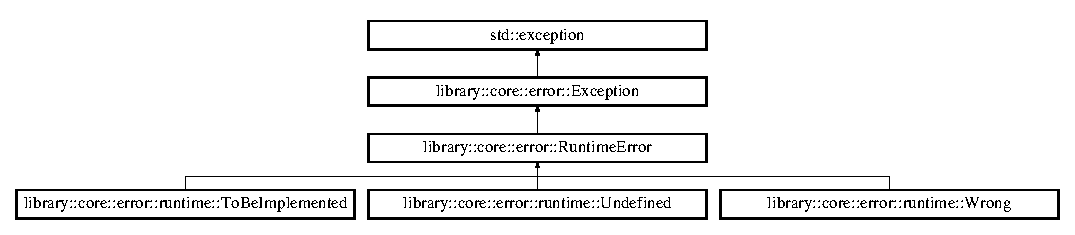
\includegraphics[height=2.715152cm]{classlibrary_1_1core_1_1error_1_1_exception}
\end{center}
\end{figure}
\subsection*{Public Member Functions}
\begin{DoxyCompactItemize}
\item 
\mbox{\Hypertarget{classlibrary_1_1core_1_1error_1_1_exception_a8e0c32779ff9a01d992d810848c841b7}\label{classlibrary_1_1core_1_1error_1_1_exception_a8e0c32779ff9a01d992d810848c841b7}} 
{\bfseries Exception} (const \hyperlink{classlibrary_1_1core_1_1types_1_1_string}{String} \&a\+Scope)
\item 
\mbox{\Hypertarget{classlibrary_1_1core_1_1error_1_1_exception_a9c20da352aa0785b837b43cd52d09500}\label{classlibrary_1_1core_1_1error_1_1_exception_a9c20da352aa0785b837b43cd52d09500}} 
\hyperlink{classlibrary_1_1core_1_1types_1_1_string}{String} {\bfseries get\+Scope} () const
\item 
\mbox{\Hypertarget{classlibrary_1_1core_1_1error_1_1_exception_ab318a927162519b15961ca66be07fd6b}\label{classlibrary_1_1core_1_1error_1_1_exception_ab318a927162519b15961ca66be07fd6b}} 
virtual const char $\ast$ {\bfseries what} () const noexcept
\end{DoxyCompactItemize}


\subsection{Detailed Description}
\hyperlink{classlibrary_1_1core_1_1error_1_1_exception}{Exception} class. 

The documentation for this class was generated from the following files\+:\begin{DoxyCompactItemize}
\item 
include/\+Library/\+Core/\+Error/\hyperlink{_exception_8hpp}{Exception.\+hpp}\item 
src/\+Library/\+Core/\+Error/\hyperlink{_exception_8cpp}{Exception.\+cpp}\end{DoxyCompactItemize}

\hypertarget{classlibrary_1_1core_1_1fs_1_1_file}{}\section{library\+:\+:core\+:\+:fs\+:\+:File Class Reference}
\label{classlibrary_1_1core_1_1fs_1_1_file}\index{library\+::core\+::fs\+::\+File@{library\+::core\+::fs\+::\+File}}


Computer resource for recording data discretely in a computer storage device.  




{\ttfamily \#include $<$File.\+hpp$>$}

\subsection*{Public Member Functions}
\begin{DoxyCompactItemize}
\item 
\hyperlink{classlibrary_1_1core_1_1fs_1_1_file_a6f3f0d79545ac9984c6f49432f0c6c39}{File} (const \hyperlink{classlibrary_1_1core_1_1fs_1_1_file}{File} \&a\+File)
\begin{DoxyCompactList}\small\item\em Copy constructor. \end{DoxyCompactList}\item 
\hyperlink{classlibrary_1_1core_1_1fs_1_1_file}{File} \& \hyperlink{classlibrary_1_1core_1_1fs_1_1_file_a8143d55e67cf2d6256c7653619a03909}{operator=} (const \hyperlink{classlibrary_1_1core_1_1fs_1_1_file}{File} \&a\+File)
\begin{DoxyCompactList}\small\item\em Copy assignment operator. \end{DoxyCompactList}\item 
bool \hyperlink{classlibrary_1_1core_1_1fs_1_1_file_a44ab79a23c5a129be298a026dbeec62f}{operator==} (const \hyperlink{classlibrary_1_1core_1_1fs_1_1_file}{File} \&a\+File) const
\begin{DoxyCompactList}\small\item\em Equal to operator. \end{DoxyCompactList}\item 
bool \hyperlink{classlibrary_1_1core_1_1fs_1_1_file_a0354b6dd59250c07cd5a8b679dc36d95}{operator!=} (const \hyperlink{classlibrary_1_1core_1_1fs_1_1_file}{File} \&a\+File) const
\begin{DoxyCompactList}\small\item\em Not equal to operator. \end{DoxyCompactList}\item 
bool \hyperlink{classlibrary_1_1core_1_1fs_1_1_file_a2044eecd956aaf55b4c55872485e1bf9}{is\+Defined} () const
\begin{DoxyCompactList}\small\item\em Check if file is defined. \end{DoxyCompactList}\item 
bool \hyperlink{classlibrary_1_1core_1_1fs_1_1_file_a61851886b6bf66cd0f179b6c7bd7f972}{exists} () const
\begin{DoxyCompactList}\small\item\em Check if file exists. \end{DoxyCompactList}\item 
\hyperlink{classlibrary_1_1core_1_1types_1_1_string}{String} \hyperlink{classlibrary_1_1core_1_1fs_1_1_file_ac8ecef1fd249eaf2ab6d7141131c0424}{get\+Name} (bool with\+Extension=true) const
\begin{DoxyCompactList}\small\item\em Get file name. \end{DoxyCompactList}\item 
\hyperlink{classlibrary_1_1core_1_1types_1_1_string}{String} \hyperlink{classlibrary_1_1core_1_1fs_1_1_file_acfb85ab6934afc65ecf53a1a08775f84}{get\+Extension} () const
\begin{DoxyCompactList}\small\item\em Get file extension. \end{DoxyCompactList}\item 
\hyperlink{classlibrary_1_1core_1_1fs_1_1_path}{fs\+::\+Path} \hyperlink{classlibrary_1_1core_1_1fs_1_1_file_a70b1380ff844adf37a481bbdb46d11a0}{get\+Path} () const
\begin{DoxyCompactList}\small\item\em Get file path. \end{DoxyCompactList}\item 
\hyperlink{classlibrary_1_1core_1_1fs_1_1_permission_set}{fs\+::\+Permission\+Set} \hyperlink{classlibrary_1_1core_1_1fs_1_1_file_a0addf18f7510955e48fdef2416b98423}{get\+Permissions} () const
\begin{DoxyCompactList}\small\item\em Get file permissions. \end{DoxyCompactList}\item 
\hyperlink{classlibrary_1_1core_1_1fs_1_1_directory}{fs\+::\+Directory} \hyperlink{classlibrary_1_1core_1_1fs_1_1_file_a8eb74097f9bdc9d3c626fe4924bf405e}{get\+Parent\+Directory} () const
\begin{DoxyCompactList}\small\item\em Get file\textquotesingle{}s parent directory. \end{DoxyCompactList}\item 
\hyperlink{classlibrary_1_1core_1_1types_1_1_string}{String} \hyperlink{classlibrary_1_1core_1_1fs_1_1_file_a0a48a4d886d255e53e35511f1519e7fa}{get\+Contents} () const
\item 
\hyperlink{classlibrary_1_1core_1_1types_1_1_string}{String} \hyperlink{classlibrary_1_1core_1_1fs_1_1_file_a891360e0ec67f357b528b3a1827d8c21}{to\+String} () const
\begin{DoxyCompactList}\small\item\em Get serialized file. \end{DoxyCompactList}\item 
void \hyperlink{classlibrary_1_1core_1_1fs_1_1_file_ae65190a612b6958e9e36238e3370c134}{rename\+To} (const \hyperlink{classlibrary_1_1core_1_1types_1_1_string}{String} \&a\+Name)
\begin{DoxyCompactList}\small\item\em Rename file. \end{DoxyCompactList}\item 
\hyperlink{classlibrary_1_1core_1_1fs_1_1_file}{File} \hyperlink{classlibrary_1_1core_1_1fs_1_1_file_a9fd8a0cca72e2414f071d6045c0a1a0d}{copy\+To\+Directory} (const \hyperlink{classlibrary_1_1core_1_1fs_1_1_directory}{fs\+::\+Directory} \&a\+Destination, const \hyperlink{classlibrary_1_1core_1_1types_1_1_string}{String} \&a\+New\+File\+Name=\char`\"{}\char`\"{}) const
\begin{DoxyCompactList}\small\item\em Copy file to directory. \end{DoxyCompactList}\item 
void \hyperlink{classlibrary_1_1core_1_1fs_1_1_file_ac81efdfeb17ea50abe23d96f69bc15ae}{move\+To\+Directory} (const \hyperlink{classlibrary_1_1core_1_1fs_1_1_directory}{fs\+::\+Directory} \&a\+Destination)
\begin{DoxyCompactList}\small\item\em Move file to directory. \end{DoxyCompactList}\item 
void \hyperlink{classlibrary_1_1core_1_1fs_1_1_file_aa83b1f11be8c9106e780266dc097d03c}{create} (const \hyperlink{classlibrary_1_1core_1_1fs_1_1_permission_set}{fs\+::\+Permission\+Set} \&an\+Owner\+Permissions\+Set=\hyperlink{classlibrary_1_1core_1_1fs_1_1_permission_set_a9722204cdc11a0171e1a115d449a134b}{fs\+::\+Permission\+Set\+::\+RW}(), const \hyperlink{classlibrary_1_1core_1_1fs_1_1_permission_set}{fs\+::\+Permission\+Set} \&a\+Group\+Permissions\+Set=\hyperlink{classlibrary_1_1core_1_1fs_1_1_permission_set_a48d447273c118d6a7c81aebb505189c6}{fs\+::\+Permission\+Set\+::R}(), const \hyperlink{classlibrary_1_1core_1_1fs_1_1_permission_set}{fs\+::\+Permission\+Set} \&an\+Other\+Permissions\+Set=\hyperlink{classlibrary_1_1core_1_1fs_1_1_permission_set_a48d447273c118d6a7c81aebb505189c6}{fs\+::\+Permission\+Set\+::R}())
\begin{DoxyCompactList}\small\item\em Create empty file. \end{DoxyCompactList}\item 
void \hyperlink{classlibrary_1_1core_1_1fs_1_1_file_a0b95ab08dd8df2cc28b2e42a72ae0b9a}{clear} ()
\begin{DoxyCompactList}\small\item\em Clear file contents. \end{DoxyCompactList}\item 
void \hyperlink{classlibrary_1_1core_1_1fs_1_1_file_a438408d402b994d76d4de3829ec67dbc}{remove} ()
\begin{DoxyCompactList}\small\item\em Delete file. \end{DoxyCompactList}\end{DoxyCompactItemize}
\subsection*{Static Public Member Functions}
\begin{DoxyCompactItemize}
\item 
static \hyperlink{classlibrary_1_1core_1_1fs_1_1_file}{File} \hyperlink{classlibrary_1_1core_1_1fs_1_1_file_af45fa5c36c359a979149845ef06586e6}{Undefined} ()
\begin{DoxyCompactList}\small\item\em Constructs an undefined file. \end{DoxyCompactList}\item 
static \hyperlink{classlibrary_1_1core_1_1fs_1_1_file}{File} \hyperlink{classlibrary_1_1core_1_1fs_1_1_file_a72d6cdf8bb7e299889c6149e2b8a6cc7}{Path} (const \hyperlink{classlibrary_1_1core_1_1fs_1_1_path}{fs\+::\+Path} \&a\+Path)
\begin{DoxyCompactList}\small\item\em Constructs a file from a given path. \end{DoxyCompactList}\end{DoxyCompactItemize}
\subsection*{Friends}
\begin{DoxyCompactItemize}
\item 
std\+::ostream \& \hyperlink{classlibrary_1_1core_1_1fs_1_1_file_a82ce9f27653427d53ecb90de978f4f68}{operator$<$$<$} (std\+::ostream \&an\+Output\+Stream, const \hyperlink{classlibrary_1_1core_1_1fs_1_1_file}{File} \&a\+File)
\begin{DoxyCompactList}\small\item\em Output stream operator. \end{DoxyCompactList}\end{DoxyCompactItemize}


\subsection{Detailed Description}
Computer resource for recording data discretely in a computer storage device. 

\subsection{Constructor \& Destructor Documentation}
\mbox{\Hypertarget{classlibrary_1_1core_1_1fs_1_1_file_a6f3f0d79545ac9984c6f49432f0c6c39}\label{classlibrary_1_1core_1_1fs_1_1_file_a6f3f0d79545ac9984c6f49432f0c6c39}} 
\index{library\+::core\+::fs\+::\+File@{library\+::core\+::fs\+::\+File}!File@{File}}
\index{File@{File}!library\+::core\+::fs\+::\+File@{library\+::core\+::fs\+::\+File}}
\subsubsection{\texorpdfstring{File()}{File()}}
{\footnotesize\ttfamily library\+::core\+::fs\+::\+File\+::\+File (\begin{DoxyParamCaption}\item[{const \hyperlink{classlibrary_1_1core_1_1fs_1_1_file}{File} \&}]{a\+File }\end{DoxyParamCaption})}



Copy constructor. 


\begin{DoxyParams}[1]{Parameters}
\mbox{\tt in}  & {\em a\+File} & A file \\
\hline
\end{DoxyParams}


\subsection{Member Function Documentation}
\mbox{\Hypertarget{classlibrary_1_1core_1_1fs_1_1_file_a0b95ab08dd8df2cc28b2e42a72ae0b9a}\label{classlibrary_1_1core_1_1fs_1_1_file_a0b95ab08dd8df2cc28b2e42a72ae0b9a}} 
\index{library\+::core\+::fs\+::\+File@{library\+::core\+::fs\+::\+File}!clear@{clear}}
\index{clear@{clear}!library\+::core\+::fs\+::\+File@{library\+::core\+::fs\+::\+File}}
\subsubsection{\texorpdfstring{clear()}{clear()}}
{\footnotesize\ttfamily void library\+::core\+::fs\+::\+File\+::clear (\begin{DoxyParamCaption}{ }\end{DoxyParamCaption})}



Clear file contents. 


\begin{DoxyCode}
\hyperlink{classlibrary_1_1core_1_1fs_1_1_file_a6f3f0d79545ac9984c6f49432f0c6c39}{File} file = \hyperlink{classlibrary_1_1core_1_1fs_1_1_file_a72d6cdf8bb7e299889c6149e2b8a6cc7}{File::Path}(\hyperlink{classlibrary_1_1core_1_1fs_1_1_path_a6ba644b6609507e724c217bf2020f5ae}{Path::Parse}(\textcolor{stringliteral}{"/path/to/file.txt"})) ;
file.exists() ; \textcolor{comment}{// True}
file.clear() ;
file.exists() ; \textcolor{comment}{// True}
\end{DoxyCode}
 \mbox{\Hypertarget{classlibrary_1_1core_1_1fs_1_1_file_a9fd8a0cca72e2414f071d6045c0a1a0d}\label{classlibrary_1_1core_1_1fs_1_1_file_a9fd8a0cca72e2414f071d6045c0a1a0d}} 
\index{library\+::core\+::fs\+::\+File@{library\+::core\+::fs\+::\+File}!copy\+To\+Directory@{copy\+To\+Directory}}
\index{copy\+To\+Directory@{copy\+To\+Directory}!library\+::core\+::fs\+::\+File@{library\+::core\+::fs\+::\+File}}
\subsubsection{\texorpdfstring{copy\+To\+Directory()}{copyToDirectory()}}
{\footnotesize\ttfamily \hyperlink{classlibrary_1_1core_1_1fs_1_1_file}{File} library\+::core\+::fs\+::\+File\+::copy\+To\+Directory (\begin{DoxyParamCaption}\item[{const \hyperlink{classlibrary_1_1core_1_1fs_1_1_directory}{fs\+::\+Directory} \&}]{a\+Destination,  }\item[{const \hyperlink{classlibrary_1_1core_1_1types_1_1_string}{String} \&}]{a\+New\+File\+Name = {\ttfamily \char`\"{}\char`\"{}} }\end{DoxyParamCaption}) const}



Copy file to directory. 


\begin{DoxyCode}
\hyperlink{classlibrary_1_1core_1_1fs_1_1_file_a6f3f0d79545ac9984c6f49432f0c6c39}{File} original = \hyperlink{classlibrary_1_1core_1_1fs_1_1_file_a72d6cdf8bb7e299889c6149e2b8a6cc7}{File::Path}(\hyperlink{classlibrary_1_1core_1_1fs_1_1_path_a6ba644b6609507e724c217bf2020f5ae}{Path::Parse}(\textcolor{stringliteral}{"/path/to/file.txt"})) ;
Directory destination = \hyperlink{classlibrary_1_1core_1_1fs_1_1_directory_a6d3ea04654841e62a4dbd99feb563caf}{Directory::Path}(\hyperlink{classlibrary_1_1core_1_1fs_1_1_path_a6ba644b6609507e724c217bf2020f5ae}{Path::Parse}(\textcolor{stringliteral}{"/new/path/to"})) ;
\hyperlink{classlibrary_1_1core_1_1fs_1_1_file_a6f3f0d79545ac9984c6f49432f0c6c39}{File} copy = original.copyToDirectory(destination) ; \textcolor{comment}{// /new/path/to/file.txt}
\end{DoxyCode}



\begin{DoxyParams}[1]{Parameters}
\mbox{\tt in}  & {\em a\+Destination} & A destination directory \\
\hline
\mbox{\tt in}  & {\em (optional)} & a\+New\+File\+Name A copied file name \\
\hline
\end{DoxyParams}
\begin{DoxyReturn}{Returns}
Copied file 
\end{DoxyReturn}
\mbox{\Hypertarget{classlibrary_1_1core_1_1fs_1_1_file_aa83b1f11be8c9106e780266dc097d03c}\label{classlibrary_1_1core_1_1fs_1_1_file_aa83b1f11be8c9106e780266dc097d03c}} 
\index{library\+::core\+::fs\+::\+File@{library\+::core\+::fs\+::\+File}!create@{create}}
\index{create@{create}!library\+::core\+::fs\+::\+File@{library\+::core\+::fs\+::\+File}}
\subsubsection{\texorpdfstring{create()}{create()}}
{\footnotesize\ttfamily void library\+::core\+::fs\+::\+File\+::create (\begin{DoxyParamCaption}\item[{const \hyperlink{classlibrary_1_1core_1_1fs_1_1_permission_set}{fs\+::\+Permission\+Set} \&}]{an\+Owner\+Permissions\+Set = {\ttfamily \hyperlink{classlibrary_1_1core_1_1fs_1_1_permission_set_a9722204cdc11a0171e1a115d449a134b}{fs\+::\+Permission\+Set\+::\+RW}()},  }\item[{const \hyperlink{classlibrary_1_1core_1_1fs_1_1_permission_set}{fs\+::\+Permission\+Set} \&}]{a\+Group\+Permissions\+Set = {\ttfamily \hyperlink{classlibrary_1_1core_1_1fs_1_1_permission_set_a48d447273c118d6a7c81aebb505189c6}{fs\+::\+Permission\+Set\+::R}()},  }\item[{const \hyperlink{classlibrary_1_1core_1_1fs_1_1_permission_set}{fs\+::\+Permission\+Set} \&}]{an\+Other\+Permissions\+Set = {\ttfamily \hyperlink{classlibrary_1_1core_1_1fs_1_1_permission_set_a48d447273c118d6a7c81aebb505189c6}{fs\+::\+Permission\+Set\+::R}()} }\end{DoxyParamCaption})}



Create empty file. 


\begin{DoxyCode}
\hyperlink{classlibrary_1_1core_1_1fs_1_1_file_a6f3f0d79545ac9984c6f49432f0c6c39}{File} file = \hyperlink{classlibrary_1_1core_1_1fs_1_1_file_a72d6cdf8bb7e299889c6149e2b8a6cc7}{File::Path}(\hyperlink{classlibrary_1_1core_1_1fs_1_1_path_a6ba644b6609507e724c217bf2020f5ae}{Path::Parse}(\textcolor{stringliteral}{"/path/to/file.txt"})) ;
file.exists() ; \textcolor{comment}{// False}
file.create() ;
file.exists() ; \textcolor{comment}{// True}
\end{DoxyCode}



\begin{DoxyParams}[1]{Parameters}
\mbox{\tt in}  & {\em (optional)} & an\+Owner\+Permissions\+Set An owner permissions set \\
\hline
\mbox{\tt in}  & {\em (optional)} & a\+Group\+Permissions\+Set A group permissions set \\
\hline
\mbox{\tt in}  & {\em (optional)} & an\+Other\+Permissions\+Set An other permissions set \\
\hline
\end{DoxyParams}
\mbox{\Hypertarget{classlibrary_1_1core_1_1fs_1_1_file_a61851886b6bf66cd0f179b6c7bd7f972}\label{classlibrary_1_1core_1_1fs_1_1_file_a61851886b6bf66cd0f179b6c7bd7f972}} 
\index{library\+::core\+::fs\+::\+File@{library\+::core\+::fs\+::\+File}!exists@{exists}}
\index{exists@{exists}!library\+::core\+::fs\+::\+File@{library\+::core\+::fs\+::\+File}}
\subsubsection{\texorpdfstring{exists()}{exists()}}
{\footnotesize\ttfamily bool library\+::core\+::fs\+::\+File\+::exists (\begin{DoxyParamCaption}{ }\end{DoxyParamCaption}) const}



Check if file exists. 


\begin{DoxyCode}
\hyperlink{classlibrary_1_1core_1_1fs_1_1_file_a6f3f0d79545ac9984c6f49432f0c6c39}{File} file = \hyperlink{classlibrary_1_1core_1_1fs_1_1_file_a72d6cdf8bb7e299889c6149e2b8a6cc7}{File::Path}(\hyperlink{classlibrary_1_1core_1_1fs_1_1_path_a6ba644b6609507e724c217bf2020f5ae}{Path::Parse}(\textcolor{stringliteral}{"/path/to/nonexistent/file"})) ;
file.exists() ; \textcolor{comment}{// False}
\end{DoxyCode}


\begin{DoxyReturn}{Returns}
True if file exists 
\end{DoxyReturn}
\mbox{\Hypertarget{classlibrary_1_1core_1_1fs_1_1_file_a0a48a4d886d255e53e35511f1519e7fa}\label{classlibrary_1_1core_1_1fs_1_1_file_a0a48a4d886d255e53e35511f1519e7fa}} 
\index{library\+::core\+::fs\+::\+File@{library\+::core\+::fs\+::\+File}!get\+Contents@{get\+Contents}}
\index{get\+Contents@{get\+Contents}!library\+::core\+::fs\+::\+File@{library\+::core\+::fs\+::\+File}}
\subsubsection{\texorpdfstring{get\+Contents()}{getContents()}}
{\footnotesize\ttfamily \hyperlink{classlibrary_1_1core_1_1types_1_1_string}{String} library\+::core\+::fs\+::\+File\+::get\+Contents (\begin{DoxyParamCaption}{ }\end{DoxyParamCaption}) const}

\mbox{\Hypertarget{classlibrary_1_1core_1_1fs_1_1_file_acfb85ab6934afc65ecf53a1a08775f84}\label{classlibrary_1_1core_1_1fs_1_1_file_acfb85ab6934afc65ecf53a1a08775f84}} 
\index{library\+::core\+::fs\+::\+File@{library\+::core\+::fs\+::\+File}!get\+Extension@{get\+Extension}}
\index{get\+Extension@{get\+Extension}!library\+::core\+::fs\+::\+File@{library\+::core\+::fs\+::\+File}}
\subsubsection{\texorpdfstring{get\+Extension()}{getExtension()}}
{\footnotesize\ttfamily \hyperlink{classlibrary_1_1core_1_1types_1_1_string}{String} library\+::core\+::fs\+::\+File\+::get\+Extension (\begin{DoxyParamCaption}{ }\end{DoxyParamCaption}) const}



Get file extension. 


\begin{DoxyCode}
\hyperlink{classlibrary_1_1core_1_1fs_1_1_file_a6f3f0d79545ac9984c6f49432f0c6c39}{File} file = \hyperlink{classlibrary_1_1core_1_1fs_1_1_file_a72d6cdf8bb7e299889c6149e2b8a6cc7}{File::Path}(\hyperlink{classlibrary_1_1core_1_1fs_1_1_path_a6ba644b6609507e724c217bf2020f5ae}{Path::Parse}(\textcolor{stringliteral}{"/path/to/file.txt"})) ;
file.getExtension() ; \textcolor{comment}{// txt}
\end{DoxyCode}


\begin{DoxyReturn}{Returns}
\hyperlink{classlibrary_1_1core_1_1fs_1_1_file}{File} extension 
\end{DoxyReturn}
\mbox{\Hypertarget{classlibrary_1_1core_1_1fs_1_1_file_ac8ecef1fd249eaf2ab6d7141131c0424}\label{classlibrary_1_1core_1_1fs_1_1_file_ac8ecef1fd249eaf2ab6d7141131c0424}} 
\index{library\+::core\+::fs\+::\+File@{library\+::core\+::fs\+::\+File}!get\+Name@{get\+Name}}
\index{get\+Name@{get\+Name}!library\+::core\+::fs\+::\+File@{library\+::core\+::fs\+::\+File}}
\subsubsection{\texorpdfstring{get\+Name()}{getName()}}
{\footnotesize\ttfamily \hyperlink{classlibrary_1_1core_1_1types_1_1_string}{String} library\+::core\+::fs\+::\+File\+::get\+Name (\begin{DoxyParamCaption}\item[{bool}]{with\+Extension = {\ttfamily true} }\end{DoxyParamCaption}) const}



Get file name. 


\begin{DoxyCode}
\hyperlink{classlibrary_1_1core_1_1fs_1_1_file_a6f3f0d79545ac9984c6f49432f0c6c39}{File} file = \hyperlink{classlibrary_1_1core_1_1fs_1_1_file_a72d6cdf8bb7e299889c6149e2b8a6cc7}{File::Path}(\hyperlink{classlibrary_1_1core_1_1fs_1_1_path_a6ba644b6609507e724c217bf2020f5ae}{Path::Parse}(\textcolor{stringliteral}{"/path/to/file.txt"})) ;
file.getName() ; \textcolor{comment}{// file.txt}
file.getName(\textcolor{keyword}{false}) ; \textcolor{comment}{// file}
\end{DoxyCode}



\begin{DoxyParams}[1]{Parameters}
\mbox{\tt in}  & {\em (optional)} & with\+Extension If true, add extension to filename \\
\hline
\end{DoxyParams}
\begin{DoxyReturn}{Returns}
\hyperlink{classlibrary_1_1core_1_1fs_1_1_file}{File} name 
\end{DoxyReturn}
\mbox{\Hypertarget{classlibrary_1_1core_1_1fs_1_1_file_a8eb74097f9bdc9d3c626fe4924bf405e}\label{classlibrary_1_1core_1_1fs_1_1_file_a8eb74097f9bdc9d3c626fe4924bf405e}} 
\index{library\+::core\+::fs\+::\+File@{library\+::core\+::fs\+::\+File}!get\+Parent\+Directory@{get\+Parent\+Directory}}
\index{get\+Parent\+Directory@{get\+Parent\+Directory}!library\+::core\+::fs\+::\+File@{library\+::core\+::fs\+::\+File}}
\subsubsection{\texorpdfstring{get\+Parent\+Directory()}{getParentDirectory()}}
{\footnotesize\ttfamily \hyperlink{classlibrary_1_1core_1_1fs_1_1_directory}{fs\+::\+Directory} library\+::core\+::fs\+::\+File\+::get\+Parent\+Directory (\begin{DoxyParamCaption}{ }\end{DoxyParamCaption}) const}



Get file\textquotesingle{}s parent directory. 


\begin{DoxyCode}
\hyperlink{classlibrary_1_1core_1_1fs_1_1_file_a6f3f0d79545ac9984c6f49432f0c6c39}{File} file = \hyperlink{classlibrary_1_1core_1_1fs_1_1_file_a72d6cdf8bb7e299889c6149e2b8a6cc7}{File::Path}(\hyperlink{classlibrary_1_1core_1_1fs_1_1_path_a6ba644b6609507e724c217bf2020f5ae}{Path::Parse}(\textcolor{stringliteral}{"/path/to/file.txt"})) ;
Directory directory = file.getParentDirectory() ; \textcolor{comment}{// /path/to}
\end{DoxyCode}


\begin{DoxyReturn}{Returns}
\hyperlink{classlibrary_1_1core_1_1fs_1_1_file}{File}\textquotesingle{}s parent directory 
\end{DoxyReturn}
\mbox{\Hypertarget{classlibrary_1_1core_1_1fs_1_1_file_a70b1380ff844adf37a481bbdb46d11a0}\label{classlibrary_1_1core_1_1fs_1_1_file_a70b1380ff844adf37a481bbdb46d11a0}} 
\index{library\+::core\+::fs\+::\+File@{library\+::core\+::fs\+::\+File}!get\+Path@{get\+Path}}
\index{get\+Path@{get\+Path}!library\+::core\+::fs\+::\+File@{library\+::core\+::fs\+::\+File}}
\subsubsection{\texorpdfstring{get\+Path()}{getPath()}}
{\footnotesize\ttfamily \hyperlink{classlibrary_1_1core_1_1fs_1_1_path}{fs\+::\+Path} library\+::core\+::fs\+::\+File\+::get\+Path (\begin{DoxyParamCaption}{ }\end{DoxyParamCaption}) const}



Get file path. 


\begin{DoxyCode}
\hyperlink{classlibrary_1_1core_1_1fs_1_1_file_a6f3f0d79545ac9984c6f49432f0c6c39}{File} file = \hyperlink{classlibrary_1_1core_1_1fs_1_1_file_a72d6cdf8bb7e299889c6149e2b8a6cc7}{File::Path}(\hyperlink{classlibrary_1_1core_1_1fs_1_1_path_a6ba644b6609507e724c217bf2020f5ae}{Path::Parse}(\textcolor{stringliteral}{"/path/to/file.txt"})) ;
\hyperlink{classlibrary_1_1core_1_1fs_1_1_file_a72d6cdf8bb7e299889c6149e2b8a6cc7}{Path} path = file.\hyperlink{classlibrary_1_1core_1_1fs_1_1_file_a70b1380ff844adf37a481bbdb46d11a0}{getPath}() ; \textcolor{comment}{// /path/to/file.txt}
\end{DoxyCode}


\begin{DoxyReturn}{Returns}
\hyperlink{classlibrary_1_1core_1_1fs_1_1_file}{File} path 
\end{DoxyReturn}
\mbox{\Hypertarget{classlibrary_1_1core_1_1fs_1_1_file_a0addf18f7510955e48fdef2416b98423}\label{classlibrary_1_1core_1_1fs_1_1_file_a0addf18f7510955e48fdef2416b98423}} 
\index{library\+::core\+::fs\+::\+File@{library\+::core\+::fs\+::\+File}!get\+Permissions@{get\+Permissions}}
\index{get\+Permissions@{get\+Permissions}!library\+::core\+::fs\+::\+File@{library\+::core\+::fs\+::\+File}}
\subsubsection{\texorpdfstring{get\+Permissions()}{getPermissions()}}
{\footnotesize\ttfamily \hyperlink{classlibrary_1_1core_1_1fs_1_1_permission_set}{fs\+::\+Permission\+Set} library\+::core\+::fs\+::\+File\+::get\+Permissions (\begin{DoxyParamCaption}{ }\end{DoxyParamCaption}) const}



Get file permissions. 


\begin{DoxyCode}
\hyperlink{classlibrary_1_1core_1_1fs_1_1_file_a6f3f0d79545ac9984c6f49432f0c6c39}{File} file = \hyperlink{classlibrary_1_1core_1_1fs_1_1_file_a72d6cdf8bb7e299889c6149e2b8a6cc7}{File::Path}(\hyperlink{classlibrary_1_1core_1_1fs_1_1_path_a6ba644b6609507e724c217bf2020f5ae}{Path::Parse}(\textcolor{stringliteral}{"/path/to/file.txt"})) ;
Permissions permissions = file.getPermissions() ; \textcolor{comment}{// rw-}
\end{DoxyCode}


\begin{DoxyReturn}{Returns}
\hyperlink{classlibrary_1_1core_1_1fs_1_1_file}{File} permissions 
\end{DoxyReturn}
\mbox{\Hypertarget{classlibrary_1_1core_1_1fs_1_1_file_a2044eecd956aaf55b4c55872485e1bf9}\label{classlibrary_1_1core_1_1fs_1_1_file_a2044eecd956aaf55b4c55872485e1bf9}} 
\index{library\+::core\+::fs\+::\+File@{library\+::core\+::fs\+::\+File}!is\+Defined@{is\+Defined}}
\index{is\+Defined@{is\+Defined}!library\+::core\+::fs\+::\+File@{library\+::core\+::fs\+::\+File}}
\subsubsection{\texorpdfstring{is\+Defined()}{isDefined()}}
{\footnotesize\ttfamily bool library\+::core\+::fs\+::\+File\+::is\+Defined (\begin{DoxyParamCaption}{ }\end{DoxyParamCaption}) const}



Check if file is defined. 


\begin{DoxyCode}
\hyperlink{classlibrary_1_1core_1_1fs_1_1_file_a6f3f0d79545ac9984c6f49432f0c6c39}{File} file = \hyperlink{classlibrary_1_1core_1_1fs_1_1_file_af45fa5c36c359a979149845ef06586e6}{File::Undefined}() ;
file.isDefined() ; \textcolor{comment}{// False}
\end{DoxyCode}


\begin{DoxyReturn}{Returns}
True if file is defined 
\end{DoxyReturn}
\mbox{\Hypertarget{classlibrary_1_1core_1_1fs_1_1_file_ac81efdfeb17ea50abe23d96f69bc15ae}\label{classlibrary_1_1core_1_1fs_1_1_file_ac81efdfeb17ea50abe23d96f69bc15ae}} 
\index{library\+::core\+::fs\+::\+File@{library\+::core\+::fs\+::\+File}!move\+To\+Directory@{move\+To\+Directory}}
\index{move\+To\+Directory@{move\+To\+Directory}!library\+::core\+::fs\+::\+File@{library\+::core\+::fs\+::\+File}}
\subsubsection{\texorpdfstring{move\+To\+Directory()}{moveToDirectory()}}
{\footnotesize\ttfamily void library\+::core\+::fs\+::\+File\+::move\+To\+Directory (\begin{DoxyParamCaption}\item[{const \hyperlink{classlibrary_1_1core_1_1fs_1_1_directory}{fs\+::\+Directory} \&}]{a\+Destination }\end{DoxyParamCaption})}



Move file to directory. 


\begin{DoxyCode}
\hyperlink{classlibrary_1_1core_1_1fs_1_1_file_a6f3f0d79545ac9984c6f49432f0c6c39}{File} file = \hyperlink{classlibrary_1_1core_1_1fs_1_1_file_a72d6cdf8bb7e299889c6149e2b8a6cc7}{File::Path}(\hyperlink{classlibrary_1_1core_1_1fs_1_1_path_a6ba644b6609507e724c217bf2020f5ae}{Path::Parse}(\textcolor{stringliteral}{"/path/to/file.txt"})) ;
Directory destination = \hyperlink{classlibrary_1_1core_1_1fs_1_1_directory_a6d3ea04654841e62a4dbd99feb563caf}{Directory::Path}(\hyperlink{classlibrary_1_1core_1_1fs_1_1_path_a6ba644b6609507e724c217bf2020f5ae}{Path::Parse}(\textcolor{stringliteral}{"/new/path/to"})) ;
file.moveToDirectory(destination) ; \textcolor{comment}{// /new/path/to/file.txt}
\end{DoxyCode}



\begin{DoxyParams}[1]{Parameters}
\mbox{\tt in}  & {\em a\+Destination} & A destination directory \\
\hline
\end{DoxyParams}
\mbox{\Hypertarget{classlibrary_1_1core_1_1fs_1_1_file_a0354b6dd59250c07cd5a8b679dc36d95}\label{classlibrary_1_1core_1_1fs_1_1_file_a0354b6dd59250c07cd5a8b679dc36d95}} 
\index{library\+::core\+::fs\+::\+File@{library\+::core\+::fs\+::\+File}!operator"!=@{operator"!=}}
\index{operator"!=@{operator"!=}!library\+::core\+::fs\+::\+File@{library\+::core\+::fs\+::\+File}}
\subsubsection{\texorpdfstring{operator"!=()}{operator!=()}}
{\footnotesize\ttfamily bool library\+::core\+::fs\+::\+File\+::operator!= (\begin{DoxyParamCaption}\item[{const \hyperlink{classlibrary_1_1core_1_1fs_1_1_file}{File} \&}]{a\+File }\end{DoxyParamCaption}) const}



Not equal to operator. 


\begin{DoxyCode}
\hyperlink{classlibrary_1_1core_1_1fs_1_1_file_a6f3f0d79545ac9984c6f49432f0c6c39}{File} firstFile = \hyperlink{classlibrary_1_1core_1_1fs_1_1_file_a72d6cdf8bb7e299889c6149e2b8a6cc7}{File::Path}(\hyperlink{classlibrary_1_1core_1_1fs_1_1_path_a6ba644b6609507e724c217bf2020f5ae}{Path::Parse}(\textcolor{stringliteral}{"/path/to/first/file"})) ;
\hyperlink{classlibrary_1_1core_1_1fs_1_1_file_a6f3f0d79545ac9984c6f49432f0c6c39}{File} secondFile = \hyperlink{classlibrary_1_1core_1_1fs_1_1_file_a72d6cdf8bb7e299889c6149e2b8a6cc7}{File::Path}(\hyperlink{classlibrary_1_1core_1_1fs_1_1_path_a6ba644b6609507e724c217bf2020f5ae}{Path::Parse}(\textcolor{stringliteral}{"/path/to/second/file"})) ;
firstFile != secondFile ; \textcolor{comment}{// True}
\end{DoxyCode}



\begin{DoxyParams}[1]{Parameters}
\mbox{\tt in}  & {\em a\+File} & A file \\
\hline
\end{DoxyParams}
\begin{DoxyReturn}{Returns}
True if files are not equal 
\end{DoxyReturn}
\mbox{\Hypertarget{classlibrary_1_1core_1_1fs_1_1_file_a8143d55e67cf2d6256c7653619a03909}\label{classlibrary_1_1core_1_1fs_1_1_file_a8143d55e67cf2d6256c7653619a03909}} 
\index{library\+::core\+::fs\+::\+File@{library\+::core\+::fs\+::\+File}!operator=@{operator=}}
\index{operator=@{operator=}!library\+::core\+::fs\+::\+File@{library\+::core\+::fs\+::\+File}}
\subsubsection{\texorpdfstring{operator=()}{operator=()}}
{\footnotesize\ttfamily \hyperlink{classlibrary_1_1core_1_1fs_1_1_file}{File} \& library\+::core\+::fs\+::\+File\+::operator= (\begin{DoxyParamCaption}\item[{const \hyperlink{classlibrary_1_1core_1_1fs_1_1_file}{File} \&}]{a\+File }\end{DoxyParamCaption})}



Copy assignment operator. 


\begin{DoxyParams}[1]{Parameters}
\mbox{\tt in}  & {\em a\+File} & A file \\
\hline
\end{DoxyParams}
\begin{DoxyReturn}{Returns}
\hyperlink{classlibrary_1_1core_1_1fs_1_1_file}{File} 
\end{DoxyReturn}
\mbox{\Hypertarget{classlibrary_1_1core_1_1fs_1_1_file_a44ab79a23c5a129be298a026dbeec62f}\label{classlibrary_1_1core_1_1fs_1_1_file_a44ab79a23c5a129be298a026dbeec62f}} 
\index{library\+::core\+::fs\+::\+File@{library\+::core\+::fs\+::\+File}!operator==@{operator==}}
\index{operator==@{operator==}!library\+::core\+::fs\+::\+File@{library\+::core\+::fs\+::\+File}}
\subsubsection{\texorpdfstring{operator==()}{operator==()}}
{\footnotesize\ttfamily bool library\+::core\+::fs\+::\+File\+::operator== (\begin{DoxyParamCaption}\item[{const \hyperlink{classlibrary_1_1core_1_1fs_1_1_file}{File} \&}]{a\+File }\end{DoxyParamCaption}) const}



Equal to operator. 


\begin{DoxyCode}
\hyperlink{classlibrary_1_1core_1_1fs_1_1_file_a6f3f0d79545ac9984c6f49432f0c6c39}{File} firstFile = \hyperlink{classlibrary_1_1core_1_1fs_1_1_file_a72d6cdf8bb7e299889c6149e2b8a6cc7}{File::Path}(\hyperlink{classlibrary_1_1core_1_1fs_1_1_path_a6ba644b6609507e724c217bf2020f5ae}{Path::Parse}(\textcolor{stringliteral}{"/path/to/file"})) ;
\hyperlink{classlibrary_1_1core_1_1fs_1_1_file_a6f3f0d79545ac9984c6f49432f0c6c39}{File} secondFile = \hyperlink{classlibrary_1_1core_1_1fs_1_1_file_a72d6cdf8bb7e299889c6149e2b8a6cc7}{File::Path}(\hyperlink{classlibrary_1_1core_1_1fs_1_1_path_a6ba644b6609507e724c217bf2020f5ae}{Path::Parse}(\textcolor{stringliteral}{"/path/to/file"})) ;
firstFile == secondFile ; \textcolor{comment}{// True}
\end{DoxyCode}



\begin{DoxyParams}[1]{Parameters}
\mbox{\tt in}  & {\em a\+File} & A file \\
\hline
\end{DoxyParams}
\begin{DoxyReturn}{Returns}
True if files are equal 
\end{DoxyReturn}
\mbox{\Hypertarget{classlibrary_1_1core_1_1fs_1_1_file_a72d6cdf8bb7e299889c6149e2b8a6cc7}\label{classlibrary_1_1core_1_1fs_1_1_file_a72d6cdf8bb7e299889c6149e2b8a6cc7}} 
\index{library\+::core\+::fs\+::\+File@{library\+::core\+::fs\+::\+File}!Path@{Path}}
\index{Path@{Path}!library\+::core\+::fs\+::\+File@{library\+::core\+::fs\+::\+File}}
\subsubsection{\texorpdfstring{Path()}{Path()}}
{\footnotesize\ttfamily \hyperlink{classlibrary_1_1core_1_1fs_1_1_file}{File} library\+::core\+::fs\+::\+File\+::\+Path (\begin{DoxyParamCaption}\item[{const \hyperlink{classlibrary_1_1core_1_1fs_1_1_path}{fs\+::\+Path} \&}]{a\+Path }\end{DoxyParamCaption})\hspace{0.3cm}{\ttfamily [static]}}



Constructs a file from a given path. 


\begin{DoxyCode}
\hyperlink{classlibrary_1_1core_1_1fs_1_1_file_a6f3f0d79545ac9984c6f49432f0c6c39}{File} file = \hyperlink{classlibrary_1_1core_1_1fs_1_1_file_a72d6cdf8bb7e299889c6149e2b8a6cc7}{File::Path}(\hyperlink{classlibrary_1_1core_1_1fs_1_1_path_a6ba644b6609507e724c217bf2020f5ae}{Path::Parse}(\textcolor{stringliteral}{"/path/to/file.txt"})) ;
file.isDefined() ; \textcolor{comment}{// True}
\end{DoxyCode}



\begin{DoxyParams}[1]{Parameters}
\mbox{\tt in}  & {\em a\+Path} & \hyperlink{classlibrary_1_1core_1_1fs_1_1_path}{Path} to file \\
\hline
\end{DoxyParams}
\begin{DoxyReturn}{Returns}
\hyperlink{classlibrary_1_1core_1_1fs_1_1_file}{File} 
\end{DoxyReturn}
\mbox{\Hypertarget{classlibrary_1_1core_1_1fs_1_1_file_a438408d402b994d76d4de3829ec67dbc}\label{classlibrary_1_1core_1_1fs_1_1_file_a438408d402b994d76d4de3829ec67dbc}} 
\index{library\+::core\+::fs\+::\+File@{library\+::core\+::fs\+::\+File}!remove@{remove}}
\index{remove@{remove}!library\+::core\+::fs\+::\+File@{library\+::core\+::fs\+::\+File}}
\subsubsection{\texorpdfstring{remove()}{remove()}}
{\footnotesize\ttfamily void library\+::core\+::fs\+::\+File\+::remove (\begin{DoxyParamCaption}{ }\end{DoxyParamCaption})}



Delete file. 


\begin{DoxyCode}
\hyperlink{classlibrary_1_1core_1_1fs_1_1_file_a6f3f0d79545ac9984c6f49432f0c6c39}{File} file = \hyperlink{classlibrary_1_1core_1_1fs_1_1_file_a72d6cdf8bb7e299889c6149e2b8a6cc7}{File::Path}(\hyperlink{classlibrary_1_1core_1_1fs_1_1_path_a6ba644b6609507e724c217bf2020f5ae}{Path::Parse}(\textcolor{stringliteral}{"/path/to/file.txt"})) ;
file.exists() ; \textcolor{comment}{// True}
file.delete() ;
file.exists() ; \textcolor{comment}{// False}
\end{DoxyCode}
 \mbox{\Hypertarget{classlibrary_1_1core_1_1fs_1_1_file_ae65190a612b6958e9e36238e3370c134}\label{classlibrary_1_1core_1_1fs_1_1_file_ae65190a612b6958e9e36238e3370c134}} 
\index{library\+::core\+::fs\+::\+File@{library\+::core\+::fs\+::\+File}!rename\+To@{rename\+To}}
\index{rename\+To@{rename\+To}!library\+::core\+::fs\+::\+File@{library\+::core\+::fs\+::\+File}}
\subsubsection{\texorpdfstring{rename\+To()}{renameTo()}}
{\footnotesize\ttfamily void library\+::core\+::fs\+::\+File\+::rename\+To (\begin{DoxyParamCaption}\item[{const \hyperlink{classlibrary_1_1core_1_1types_1_1_string}{String} \&}]{a\+Name }\end{DoxyParamCaption})}



Rename file. 


\begin{DoxyCode}
\hyperlink{classlibrary_1_1core_1_1fs_1_1_file_a6f3f0d79545ac9984c6f49432f0c6c39}{File} file = \hyperlink{classlibrary_1_1core_1_1fs_1_1_file_a72d6cdf8bb7e299889c6149e2b8a6cc7}{File::Path}(\hyperlink{classlibrary_1_1core_1_1fs_1_1_path_a6ba644b6609507e724c217bf2020f5ae}{Path::Parse}(\textcolor{stringliteral}{"/path/to/file.txt"})) ;
file.renameTo(\textcolor{stringliteral}{"cat.jpg"}) ; \textcolor{comment}{// /path/to/cat.jpg}
\end{DoxyCode}



\begin{DoxyParams}[1]{Parameters}
\mbox{\tt in}  & {\em a\+Name} & A file name \\
\hline
\end{DoxyParams}
\mbox{\Hypertarget{classlibrary_1_1core_1_1fs_1_1_file_a891360e0ec67f357b528b3a1827d8c21}\label{classlibrary_1_1core_1_1fs_1_1_file_a891360e0ec67f357b528b3a1827d8c21}} 
\index{library\+::core\+::fs\+::\+File@{library\+::core\+::fs\+::\+File}!to\+String@{to\+String}}
\index{to\+String@{to\+String}!library\+::core\+::fs\+::\+File@{library\+::core\+::fs\+::\+File}}
\subsubsection{\texorpdfstring{to\+String()}{toString()}}
{\footnotesize\ttfamily \hyperlink{classlibrary_1_1core_1_1types_1_1_string}{String} library\+::core\+::fs\+::\+File\+::to\+String (\begin{DoxyParamCaption}{ }\end{DoxyParamCaption}) const}



Get serialized file. 


\begin{DoxyCode}
\hyperlink{classlibrary_1_1core_1_1fs_1_1_file_a72d6cdf8bb7e299889c6149e2b8a6cc7}{File::Path}(\hyperlink{classlibrary_1_1core_1_1fs_1_1_path_a6ba644b6609507e724c217bf2020f5ae}{Path::Parse}(\textcolor{stringliteral}{"/path/to/file"})).\hyperlink{classlibrary_1_1core_1_1fs_1_1_file_a891360e0ec67f357b528b3a1827d8c21}{toString}() ; \textcolor{comment}{// "/path/to/file"}
\end{DoxyCode}


\begin{DoxyReturn}{Returns}
Serialized file 
\end{DoxyReturn}
\mbox{\Hypertarget{classlibrary_1_1core_1_1fs_1_1_file_af45fa5c36c359a979149845ef06586e6}\label{classlibrary_1_1core_1_1fs_1_1_file_af45fa5c36c359a979149845ef06586e6}} 
\index{library\+::core\+::fs\+::\+File@{library\+::core\+::fs\+::\+File}!Undefined@{Undefined}}
\index{Undefined@{Undefined}!library\+::core\+::fs\+::\+File@{library\+::core\+::fs\+::\+File}}
\subsubsection{\texorpdfstring{Undefined()}{Undefined()}}
{\footnotesize\ttfamily \hyperlink{classlibrary_1_1core_1_1fs_1_1_file}{File} library\+::core\+::fs\+::\+File\+::\+Undefined (\begin{DoxyParamCaption}{ }\end{DoxyParamCaption})\hspace{0.3cm}{\ttfamily [static]}}



Constructs an undefined file. 


\begin{DoxyCode}
\hyperlink{classlibrary_1_1core_1_1fs_1_1_file_a6f3f0d79545ac9984c6f49432f0c6c39}{File} file = \hyperlink{classlibrary_1_1core_1_1fs_1_1_file_af45fa5c36c359a979149845ef06586e6}{File::Undefined}() ;
file.isDefined() ; \textcolor{comment}{// False}
\end{DoxyCode}


\begin{DoxyReturn}{Returns}
Undefined file 
\end{DoxyReturn}


\subsection{Friends And Related Function Documentation}
\mbox{\Hypertarget{classlibrary_1_1core_1_1fs_1_1_file_a82ce9f27653427d53ecb90de978f4f68}\label{classlibrary_1_1core_1_1fs_1_1_file_a82ce9f27653427d53ecb90de978f4f68}} 
\index{library\+::core\+::fs\+::\+File@{library\+::core\+::fs\+::\+File}!operator$<$$<$@{operator$<$$<$}}
\index{operator$<$$<$@{operator$<$$<$}!library\+::core\+::fs\+::\+File@{library\+::core\+::fs\+::\+File}}
\subsubsection{\texorpdfstring{operator$<$$<$}{operator<<}}
{\footnotesize\ttfamily std\+::ostream\& operator$<$$<$ (\begin{DoxyParamCaption}\item[{std\+::ostream \&}]{an\+Output\+Stream,  }\item[{const \hyperlink{classlibrary_1_1core_1_1fs_1_1_file}{File} \&}]{a\+File }\end{DoxyParamCaption})\hspace{0.3cm}{\ttfamily [friend]}}



Output stream operator. 


\begin{DoxyCode}
\hyperlink{classlibrary_1_1core_1_1fs_1_1_file_a6f3f0d79545ac9984c6f49432f0c6c39}{File} file = \hyperlink{classlibrary_1_1core_1_1fs_1_1_file_a72d6cdf8bb7e299889c6149e2b8a6cc7}{File::Path}(\hyperlink{classlibrary_1_1core_1_1fs_1_1_path_a6ba644b6609507e724c217bf2020f5ae}{Path::Parse}(\textcolor{stringliteral}{"/path/to/file"})) ;
std::cout << file ;
\end{DoxyCode}



\begin{DoxyParams}[1]{Parameters}
\mbox{\tt in}  & {\em an\+Output\+Stream} & An output stream \\
\hline
\mbox{\tt in}  & {\em a\+File} & A file \\
\hline
\end{DoxyParams}
\begin{DoxyReturn}{Returns}
An output stream 
\end{DoxyReturn}


The documentation for this class was generated from the following files\+:\begin{DoxyCompactItemize}
\item 
include/\+Library/\+Core/\+File\+System/\hyperlink{_file_8hpp}{File.\+hpp}\item 
src/\+Library/\+Core/\+File\+System/\hyperlink{_file_8cpp}{File.\+cpp}\end{DoxyCompactItemize}

\hypertarget{classlibrary_1_1core_1_1ctnr_1_1_graph}{}\section{library\+:\+:core\+:\+:ctnr\+:\+:Graph Class Reference}
\label{classlibrary_1_1core_1_1ctnr_1_1_graph}\index{library\+::core\+::ctnr\+::\+Graph@{library\+::core\+::ctnr\+::\+Graph}}


Structure consisting of a finite set of vertices, together with a set of pairs of these vertices (edges).  




{\ttfamily \#include $<$Graph.\+hpp$>$}

\subsection*{Public Member Functions}
\begin{DoxyCompactItemize}
\item 
\mbox{\Hypertarget{classlibrary_1_1core_1_1ctnr_1_1_graph_aed97aab348693c80c4cd7b4a3cf3c1ba}\label{classlibrary_1_1core_1_1ctnr_1_1_graph_aed97aab348693c80c4cd7b4a3cf3c1ba}} 
{\bfseries Graph} (const \hyperlink{classlibrary_1_1core_1_1ctnr_1_1_graph}{Graph} \&a\+Graph)
\item 
\mbox{\Hypertarget{classlibrary_1_1core_1_1ctnr_1_1_graph_ac31e1114997d3c6ab11df23e2bfede04}\label{classlibrary_1_1core_1_1ctnr_1_1_graph_ac31e1114997d3c6ab11df23e2bfede04}} 
\hyperlink{classlibrary_1_1core_1_1ctnr_1_1_graph}{Graph} \& {\bfseries operator=} (const \hyperlink{classlibrary_1_1core_1_1ctnr_1_1_graph}{Graph} \&a\+Graph) const
\item 
\mbox{\Hypertarget{classlibrary_1_1core_1_1ctnr_1_1_graph_a089dddc20bedaa9c590fca0c6e6b4677}\label{classlibrary_1_1core_1_1ctnr_1_1_graph_a089dddc20bedaa9c590fca0c6e6b4677}} 
bool {\bfseries is\+Defined} () const
\end{DoxyCompactItemize}
\subsection*{Static Public Member Functions}
\begin{DoxyCompactItemize}
\item 
\mbox{\Hypertarget{classlibrary_1_1core_1_1ctnr_1_1_graph_a36b399824e8668d7c068f0933da39731}\label{classlibrary_1_1core_1_1ctnr_1_1_graph_a36b399824e8668d7c068f0933da39731}} 
static \hyperlink{classlibrary_1_1core_1_1ctnr_1_1_graph}{Graph} {\bfseries Empty} ()
\item 
\mbox{\Hypertarget{classlibrary_1_1core_1_1ctnr_1_1_graph_a3404e53c5dffbafad666f346d3663f0d}\label{classlibrary_1_1core_1_1ctnr_1_1_graph_a3404e53c5dffbafad666f346d3663f0d}} 
static \hyperlink{classlibrary_1_1core_1_1ctnr_1_1_graph}{Graph} {\bfseries Object} (const \hyperlink{classlibrary_1_1core_1_1ctnr_1_1_object}{Object} \&an\+Object)
\end{DoxyCompactItemize}
\subsection*{Friends}
\begin{DoxyCompactItemize}
\item 
\mbox{\Hypertarget{classlibrary_1_1core_1_1ctnr_1_1_graph_a225f9b61ac2385ccf05891298c7ab6b1}\label{classlibrary_1_1core_1_1ctnr_1_1_graph_a225f9b61ac2385ccf05891298c7ab6b1}} 
std\+::ostream \& {\bfseries operator$<$$<$} (std\+::ostream \&an\+Output\+Stream, const \hyperlink{classlibrary_1_1core_1_1ctnr_1_1_graph}{Graph} \&a\+Graph)
\end{DoxyCompactItemize}


\subsection{Detailed Description}
Structure consisting of a finite set of vertices, together with a set of pairs of these vertices (edges). 

https\+://en.wikipedia.\+org/wiki/\+Graph\+\_\+(abstract\+\_\+data\+\_\+type) 

The documentation for this class was generated from the following file\+:\begin{DoxyCompactItemize}
\item 
include/\+Library/\+Core/\+Containers/\hyperlink{_graph_8hpp}{Graph.\+hpp}\end{DoxyCompactItemize}

\hypertarget{classlibrary_1_1core_1_1system_1_1_group}{}\section{library\+:\+:core\+:\+:system\+:\+:Group Class Reference}
\label{classlibrary_1_1core_1_1system_1_1_group}\index{library\+::core\+::system\+::\+Group@{library\+::core\+::system\+::\+Group}}


\hyperlink{classlibrary_1_1core_1_1system_1_1_group}{Group}.  




{\ttfamily \#include $<$Group.\+hpp$>$}

\subsection*{Public Member Functions}
\begin{DoxyCompactItemize}
\item 
\mbox{\Hypertarget{classlibrary_1_1core_1_1system_1_1_group_ad9b37c98ac79505f5fbcee71b8cf2b36}\label{classlibrary_1_1core_1_1system_1_1_group_ad9b37c98ac79505f5fbcee71b8cf2b36}} 
{\bfseries Group} (const uint \&a\+G\+ID, const \hyperlink{classlibrary_1_1core_1_1types_1_1_string}{String} \&a\+Name)
\item 
\mbox{\Hypertarget{classlibrary_1_1core_1_1system_1_1_group_aa6a21b13948d6be0e344503b9e31f3ef}\label{classlibrary_1_1core_1_1system_1_1_group_aa6a21b13948d6be0e344503b9e31f3ef}} 
{\bfseries Group} (const uint \&a\+G\+ID, const uint \&a\+E\+G\+ID, const \hyperlink{classlibrary_1_1core_1_1types_1_1_string}{String} \&a\+Name)
\item 
\mbox{\Hypertarget{classlibrary_1_1core_1_1system_1_1_group_a51f4fbabf077878249d72db242a1debb}\label{classlibrary_1_1core_1_1system_1_1_group_a51f4fbabf077878249d72db242a1debb}} 
bool {\bfseries operator==} (const \hyperlink{classlibrary_1_1core_1_1system_1_1_group}{Group} \&a\+Group) const
\item 
\mbox{\Hypertarget{classlibrary_1_1core_1_1system_1_1_group_a156a737e03a483bca163ec9da3cccb8b}\label{classlibrary_1_1core_1_1system_1_1_group_a156a737e03a483bca163ec9da3cccb8b}} 
bool {\bfseries operator!=} (const \hyperlink{classlibrary_1_1core_1_1system_1_1_group}{Group} \&a\+Group) const
\item 
\mbox{\Hypertarget{classlibrary_1_1core_1_1system_1_1_group_a5b09eed8a6cdc2f29caf7eee6ad57ef0}\label{classlibrary_1_1core_1_1system_1_1_group_a5b09eed8a6cdc2f29caf7eee6ad57ef0}} 
bool {\bfseries is\+Defined} () const
\item 
\mbox{\Hypertarget{classlibrary_1_1core_1_1system_1_1_group_a22d1dd28ab638e043d1ca1aac19af36e}\label{classlibrary_1_1core_1_1system_1_1_group_a22d1dd28ab638e043d1ca1aac19af36e}} 
int {\bfseries get\+G\+ID} () const
\item 
\mbox{\Hypertarget{classlibrary_1_1core_1_1system_1_1_group_ab9677f28eb1f6653ad9c5776d1f00c3f}\label{classlibrary_1_1core_1_1system_1_1_group_ab9677f28eb1f6653ad9c5776d1f00c3f}} 
int {\bfseries get\+E\+G\+ID} () const
\item 
\mbox{\Hypertarget{classlibrary_1_1core_1_1system_1_1_group_a45d3ee1f569a68ab4bec033cb802f6b3}\label{classlibrary_1_1core_1_1system_1_1_group_a45d3ee1f569a68ab4bec033cb802f6b3}} 
int {\bfseries get\+S\+G\+ID} () const
\item 
\mbox{\Hypertarget{classlibrary_1_1core_1_1system_1_1_group_a28d73668971941ff02c106f07b599712}\label{classlibrary_1_1core_1_1system_1_1_group_a28d73668971941ff02c106f07b599712}} 
\hyperlink{classlibrary_1_1core_1_1types_1_1_string}{String} {\bfseries get\+Name} () const
\end{DoxyCompactItemize}
\subsection*{Static Public Member Functions}
\begin{DoxyCompactItemize}
\item 
\mbox{\Hypertarget{classlibrary_1_1core_1_1system_1_1_group_a50c939824e28f2ce5a0ff7ab253689e4}\label{classlibrary_1_1core_1_1system_1_1_group_a50c939824e28f2ce5a0ff7ab253689e4}} 
static \hyperlink{classlibrary_1_1core_1_1system_1_1_group}{Group} {\bfseries Undefined} ()
\item 
\mbox{\Hypertarget{classlibrary_1_1core_1_1system_1_1_group_a90961dc55447dca842c5f0ea43778c18}\label{classlibrary_1_1core_1_1system_1_1_group_a90961dc55447dca842c5f0ea43778c18}} 
static \hyperlink{classlibrary_1_1core_1_1system_1_1_group}{Group} {\bfseries Process} ()
\item 
\mbox{\Hypertarget{classlibrary_1_1core_1_1system_1_1_group_a6f6e71dd112ccb60347fa366e61cd4e9}\label{classlibrary_1_1core_1_1system_1_1_group_a6f6e71dd112ccb60347fa366e61cd4e9}} 
static \hyperlink{classlibrary_1_1core_1_1system_1_1_group}{Group} {\bfseries G\+ID} (const uint \&a\+G\+ID)
\item 
\mbox{\Hypertarget{classlibrary_1_1core_1_1system_1_1_group_a81dda2a1d0e251b40dabbde24be380d1}\label{classlibrary_1_1core_1_1system_1_1_group_a81dda2a1d0e251b40dabbde24be380d1}} 
static \hyperlink{classlibrary_1_1core_1_1system_1_1_group}{Group} {\bfseries Name} (const \hyperlink{classlibrary_1_1core_1_1types_1_1_string}{String} \&a\+Name)
\end{DoxyCompactItemize}
\subsection*{Friends}
\begin{DoxyCompactItemize}
\item 
\mbox{\Hypertarget{classlibrary_1_1core_1_1system_1_1_group_adae6b8468d9a0cf648a52c296c6db73a}\label{classlibrary_1_1core_1_1system_1_1_group_adae6b8468d9a0cf648a52c296c6db73a}} 
std\+::ostream \& {\bfseries operator$<$$<$} (std\+::ostream \&an\+Output\+Stream, const \hyperlink{classlibrary_1_1core_1_1system_1_1_group}{Group} \&a\+Group)
\end{DoxyCompactItemize}


\subsection{Detailed Description}
\hyperlink{classlibrary_1_1core_1_1system_1_1_group}{Group}. 

P\+O\+S\+IX compliant

https\+://en.wikipedia.\+org/wiki/\+Group\+\_\+identifier 

The documentation for this class was generated from the following file\+:\begin{DoxyCompactItemize}
\item 
include/\+Library/\+Core/\+System/\hyperlink{_group_8hpp}{Group.\+hpp}\end{DoxyCompactItemize}

\hypertarget{classlibrary_1_1core_1_1types_1_1_has_to_string}{}\section{library\+:\+:core\+:\+:types\+:\+:Has\+To\+String$<$ T $>$ Class Template Reference}
\label{classlibrary_1_1core_1_1types_1_1_has_to_string}\index{library\+::core\+::types\+::\+Has\+To\+String$<$ T $>$@{library\+::core\+::types\+::\+Has\+To\+String$<$ T $>$}}


https\+://gist.github.\+com/fenbf/d2cd670704b82e2ce7fd  




{\ttfamily \#include $<$String.\+hpp$>$}

\subsection*{Public Types}
\begin{DoxyCompactItemize}
\item 
enum \{ \hyperlink{classlibrary_1_1core_1_1types_1_1_has_to_string_a66718ae4c4783afe3e8137ddbd6689afaec23beac9fd1e1c74d43c6242f649acc}{value} = sizeof(test$<$T$>$(0)) == sizeof(Yes\+Type)
 \}
\end{DoxyCompactItemize}


\subsection{Detailed Description}
\subsubsection*{template$<$typename T$>$\newline
class library\+::core\+::types\+::\+Has\+To\+String$<$ T $>$}

https\+://gist.github.\+com/fenbf/d2cd670704b82e2ce7fd 

\subsection{Member Enumeration Documentation}
\mbox{\Hypertarget{classlibrary_1_1core_1_1types_1_1_has_to_string_a66718ae4c4783afe3e8137ddbd6689af}\label{classlibrary_1_1core_1_1types_1_1_has_to_string_a66718ae4c4783afe3e8137ddbd6689af}} 
\subsubsection{\texorpdfstring{anonymous enum}{anonymous enum}}
{\footnotesize\ttfamily template$<$typename T $>$ \\
anonymous enum}

\begin{DoxyEnumFields}{Enumerator}
\raisebox{\heightof{T}}[0pt][0pt]{\index{value@{value}!library\+::core\+::types\+::\+Has\+To\+String@{library\+::core\+::types\+::\+Has\+To\+String}}\index{library\+::core\+::types\+::\+Has\+To\+String@{library\+::core\+::types\+::\+Has\+To\+String}!value@{value}}}\mbox{\Hypertarget{classlibrary_1_1core_1_1types_1_1_has_to_string_a66718ae4c4783afe3e8137ddbd6689afaec23beac9fd1e1c74d43c6242f649acc}\label{classlibrary_1_1core_1_1types_1_1_has_to_string_a66718ae4c4783afe3e8137ddbd6689afaec23beac9fd1e1c74d43c6242f649acc}} 
value&\\
\hline

\end{DoxyEnumFields}


The documentation for this class was generated from the following file\+:\begin{DoxyCompactItemize}
\item 
include/\+Library/\+Core/\+Types/\hyperlink{_string_8hpp}{String.\+hpp}\end{DoxyCompactItemize}

\hypertarget{classlibrary_1_1core_1_1types_1_1_integer}{}\section{library\+::core\+::types\+::Integer Class Reference}
\label{classlibrary_1_1core_1_1types_1_1_integer}\index{library::core::types::Integer@{library::core::types::Integer}}


\mbox{\hyperlink{classlibrary_1_1core_1_1types_1_1_integer}{Integer}} type.  




{\ttfamily \#include $<$Integer.\+hpp$>$}

\subsection*{Public Types}
\begin{DoxyCompactItemize}
\item 
typedef int32\+\_\+t \mbox{\hyperlink{classlibrary_1_1core_1_1types_1_1_integer_a623afb1580f870fd8a1997b1c12c917d}{Value\+Type}}
\end{DoxyCompactItemize}
\subsection*{Public Member Functions}
\begin{DoxyCompactItemize}
\item 
\mbox{\hyperlink{classlibrary_1_1core_1_1types_1_1_integer_a6483b1c4e13e5ed6af5e7a58347efead}{Integer}} ()=delete
\begin{DoxyCompactList}\small\item\em Default constructor (disabled) \end{DoxyCompactList}\item 
\mbox{\hyperlink{classlibrary_1_1core_1_1types_1_1_integer_ac282b8e24c1d1a43e578c5be3c70ea27}{Integer}} (\mbox{\hyperlink{classlibrary_1_1core_1_1types_1_1_integer_a623afb1580f870fd8a1997b1c12c917d}{Integer\+::\+Value\+Type}} an\+Integer)
\begin{DoxyCompactList}\small\item\em Constructor. \end{DoxyCompactList}\item 
\mbox{\hyperlink{classlibrary_1_1core_1_1types_1_1_integer_af3bcebe374c4b7b4329ed0a7fae04abd}{Integer}} (float)=delete
\begin{DoxyCompactList}\small\item\em Float constructor (disabled) \end{DoxyCompactList}\item 
\mbox{\hyperlink{classlibrary_1_1core_1_1types_1_1_integer_ab0d94d5cfc78f38f1598679015f4ab61}{Integer}} (double)=delete
\begin{DoxyCompactList}\small\item\em Double constructor (disabled) \end{DoxyCompactList}\item 
\mbox{\hyperlink{classlibrary_1_1core_1_1types_1_1_integer}{Integer}} \& \mbox{\hyperlink{classlibrary_1_1core_1_1types_1_1_integer_ab77cae94a9e6d4a405a555dd55763ea2}{operator=}} (\mbox{\hyperlink{classlibrary_1_1core_1_1types_1_1_integer_a623afb1580f870fd8a1997b1c12c917d}{Integer\+::\+Value\+Type}} an\+Integer)
\begin{DoxyCompactList}\small\item\em Copy assignment operator. \end{DoxyCompactList}\item 
bool \mbox{\hyperlink{classlibrary_1_1core_1_1types_1_1_integer_a52b3a012d6c6779773d051800daac516}{operator==}} (const \mbox{\hyperlink{classlibrary_1_1core_1_1types_1_1_integer}{Integer}} \&an\+Integer) const
\begin{DoxyCompactList}\small\item\em Equal to operator. \end{DoxyCompactList}\item 
bool \mbox{\hyperlink{classlibrary_1_1core_1_1types_1_1_integer_a9145ffb6bca8771f06a3403056466d53}{operator!=}} (const \mbox{\hyperlink{classlibrary_1_1core_1_1types_1_1_integer}{Integer}} \&an\+Integer) const
\begin{DoxyCompactList}\small\item\em Not equal to operator. \end{DoxyCompactList}\item 
bool \mbox{\hyperlink{classlibrary_1_1core_1_1types_1_1_integer_a7f179765edbdeb186cde5e869021ccb6}{operator$<$}} (const \mbox{\hyperlink{classlibrary_1_1core_1_1types_1_1_integer}{Integer}} \&an\+Integer) const
\begin{DoxyCompactList}\small\item\em Less than operator. \end{DoxyCompactList}\item 
bool \mbox{\hyperlink{classlibrary_1_1core_1_1types_1_1_integer_a57c084e8ca66e33675a706868b555962}{operator$<$=}} (const \mbox{\hyperlink{classlibrary_1_1core_1_1types_1_1_integer}{Integer}} \&an\+Integer) const
\begin{DoxyCompactList}\small\item\em Less than or equal to operator. \end{DoxyCompactList}\item 
bool \mbox{\hyperlink{classlibrary_1_1core_1_1types_1_1_integer_aa5e59aba88550137a1b120e90ab155fa}{operator$>$}} (const \mbox{\hyperlink{classlibrary_1_1core_1_1types_1_1_integer}{Integer}} \&an\+Integer) const
\begin{DoxyCompactList}\small\item\em Greater than operator. \end{DoxyCompactList}\item 
bool \mbox{\hyperlink{classlibrary_1_1core_1_1types_1_1_integer_ae565ce34bef391725beebb42269d26fe}{operator$>$=}} (const \mbox{\hyperlink{classlibrary_1_1core_1_1types_1_1_integer}{Integer}} \&an\+Integer) const
\begin{DoxyCompactList}\small\item\em Greater than or equal to operator. \end{DoxyCompactList}\item 
bool \mbox{\hyperlink{classlibrary_1_1core_1_1types_1_1_integer_a02858e726140a9e84281699a41675081}{operator==}} (const \mbox{\hyperlink{classlibrary_1_1core_1_1types_1_1_integer_a623afb1580f870fd8a1997b1c12c917d}{Integer\+::\+Value\+Type}} \&an\+Integer) const
\begin{DoxyCompactList}\small\item\em Equal to Value\+Type operator. \end{DoxyCompactList}\item 
bool \mbox{\hyperlink{classlibrary_1_1core_1_1types_1_1_integer_a9c3c4e9564a3a8da5133207f3197d3a3}{operator!=}} (const \mbox{\hyperlink{classlibrary_1_1core_1_1types_1_1_integer_a623afb1580f870fd8a1997b1c12c917d}{Integer\+::\+Value\+Type}} \&an\+Integer) const
\item 
bool \mbox{\hyperlink{classlibrary_1_1core_1_1types_1_1_integer_ad893d193755f414dd680fd867ff30ea0}{operator$<$}} (const \mbox{\hyperlink{classlibrary_1_1core_1_1types_1_1_integer_a623afb1580f870fd8a1997b1c12c917d}{Integer\+::\+Value\+Type}} \&an\+Integer) const
\item 
bool \mbox{\hyperlink{classlibrary_1_1core_1_1types_1_1_integer_a09f6844cd7557f087116a50869765eaa}{operator$<$=}} (const \mbox{\hyperlink{classlibrary_1_1core_1_1types_1_1_integer_a623afb1580f870fd8a1997b1c12c917d}{Integer\+::\+Value\+Type}} \&an\+Integer) const
\item 
bool \mbox{\hyperlink{classlibrary_1_1core_1_1types_1_1_integer_a1e0736e7d215b2ad2e7291a983490bf5}{operator$>$}} (const \mbox{\hyperlink{classlibrary_1_1core_1_1types_1_1_integer_a623afb1580f870fd8a1997b1c12c917d}{Integer\+::\+Value\+Type}} \&an\+Integer) const
\item 
bool \mbox{\hyperlink{classlibrary_1_1core_1_1types_1_1_integer_a88077b530da644e33e6346837035eb9d}{operator$>$=}} (const \mbox{\hyperlink{classlibrary_1_1core_1_1types_1_1_integer_a623afb1580f870fd8a1997b1c12c917d}{Integer\+::\+Value\+Type}} \&an\+Integer) const
\item 
\mbox{\hyperlink{classlibrary_1_1core_1_1types_1_1_integer}{Integer}} \mbox{\hyperlink{classlibrary_1_1core_1_1types_1_1_integer_ade47c7abcdbcdc8c4a369a46b7d0dcef}{operator+}} (const \mbox{\hyperlink{classlibrary_1_1core_1_1types_1_1_integer}{Integer}} \&an\+Integer) const
\item 
\mbox{\hyperlink{classlibrary_1_1core_1_1types_1_1_integer}{Integer}} \mbox{\hyperlink{classlibrary_1_1core_1_1types_1_1_integer_a728dd9f86ee7d512787f2024a7194913}{operator-\/}} (const \mbox{\hyperlink{classlibrary_1_1core_1_1types_1_1_integer}{Integer}} \&an\+Integer) const
\item 
\mbox{\hyperlink{classlibrary_1_1core_1_1types_1_1_integer}{Integer}} \mbox{\hyperlink{classlibrary_1_1core_1_1types_1_1_integer_a68d6d1c6e178a5a6760345754eb84ad4}{operator$\ast$}} (const \mbox{\hyperlink{classlibrary_1_1core_1_1types_1_1_integer}{Integer}} \&an\+Integer) const
\item 
\mbox{\hyperlink{classlibrary_1_1core_1_1types_1_1_integer}{Integer}} \mbox{\hyperlink{classlibrary_1_1core_1_1types_1_1_integer_a93e85214cbbd35628e7b57092b19dd34}{operator/}} (const \mbox{\hyperlink{classlibrary_1_1core_1_1types_1_1_integer}{Integer}} \&an\+Integer) const
\item 
\mbox{\hyperlink{classlibrary_1_1core_1_1types_1_1_integer}{Integer}} \mbox{\hyperlink{classlibrary_1_1core_1_1types_1_1_integer_aaef6b38feb77d2d901cb75546690ff19}{operator\%}} (const \mbox{\hyperlink{classlibrary_1_1core_1_1types_1_1_integer}{Integer}} \&an\+Integer) const
\item 
\mbox{\hyperlink{classlibrary_1_1core_1_1types_1_1_integer}{Integer}} \mbox{\hyperlink{classlibrary_1_1core_1_1types_1_1_integer_afe13541715633da0223c4c70b9142cf7}{operator+}} (const \mbox{\hyperlink{classlibrary_1_1core_1_1types_1_1_integer_a623afb1580f870fd8a1997b1c12c917d}{Integer\+::\+Value\+Type}} \&an\+Integer) const
\item 
\mbox{\hyperlink{classlibrary_1_1core_1_1types_1_1_integer}{Integer}} \mbox{\hyperlink{classlibrary_1_1core_1_1types_1_1_integer_a7bbe7f9e02df0f4d64df023552c109e2}{operator-\/}} (const \mbox{\hyperlink{classlibrary_1_1core_1_1types_1_1_integer_a623afb1580f870fd8a1997b1c12c917d}{Integer\+::\+Value\+Type}} \&an\+Integer) const
\item 
\mbox{\hyperlink{classlibrary_1_1core_1_1types_1_1_integer}{Integer}} \mbox{\hyperlink{classlibrary_1_1core_1_1types_1_1_integer_abb096707a917c8450171ff25803dad8f}{operator$\ast$}} (const \mbox{\hyperlink{classlibrary_1_1core_1_1types_1_1_integer_a623afb1580f870fd8a1997b1c12c917d}{Integer\+::\+Value\+Type}} \&an\+Integer) const
\item 
\mbox{\hyperlink{classlibrary_1_1core_1_1types_1_1_integer}{Integer}} \mbox{\hyperlink{classlibrary_1_1core_1_1types_1_1_integer_adb76f1b3b03af117435185eb8d9d683d}{operator/}} (const \mbox{\hyperlink{classlibrary_1_1core_1_1types_1_1_integer_a623afb1580f870fd8a1997b1c12c917d}{Integer\+::\+Value\+Type}} \&an\+Integer) const
\item 
\mbox{\hyperlink{classlibrary_1_1core_1_1types_1_1_integer}{Integer}} \mbox{\hyperlink{classlibrary_1_1core_1_1types_1_1_integer_adb57aabd90fd156b8c06517fe457fe3a}{operator\%}} (const \mbox{\hyperlink{classlibrary_1_1core_1_1types_1_1_integer_a623afb1580f870fd8a1997b1c12c917d}{Integer\+::\+Value\+Type}} \&an\+Integer) const
\item 
\mbox{\hyperlink{classlibrary_1_1core_1_1types_1_1_real}{Real}} \mbox{\hyperlink{classlibrary_1_1core_1_1types_1_1_integer_a5652ce354c58df75e9273201ee3bb399}{operator+}} (const \mbox{\hyperlink{classlibrary_1_1core_1_1types_1_1_real}{Real}} \&a\+Real) const
\item 
\mbox{\hyperlink{classlibrary_1_1core_1_1types_1_1_real}{Real}} \mbox{\hyperlink{classlibrary_1_1core_1_1types_1_1_integer_acd14824d3ca5530cd8952f3e249e310f}{operator-\/}} (const \mbox{\hyperlink{classlibrary_1_1core_1_1types_1_1_real}{Real}} \&a\+Real) const
\item 
\mbox{\hyperlink{classlibrary_1_1core_1_1types_1_1_real}{Real}} \mbox{\hyperlink{classlibrary_1_1core_1_1types_1_1_integer_a3edc207fd4799cb16eb4075fdd098efb}{operator$\ast$}} (const \mbox{\hyperlink{classlibrary_1_1core_1_1types_1_1_real}{Real}} \&a\+Real) const
\item 
\mbox{\hyperlink{classlibrary_1_1core_1_1types_1_1_real}{Real}} \mbox{\hyperlink{classlibrary_1_1core_1_1types_1_1_integer_a6724d09c95b335402fe3553a13dd725d}{operator/}} (const \mbox{\hyperlink{classlibrary_1_1core_1_1types_1_1_real}{Real}} \&a\+Real) const
\item 
\mbox{\hyperlink{classlibrary_1_1core_1_1types_1_1_integer}{Integer}} \& \mbox{\hyperlink{classlibrary_1_1core_1_1types_1_1_integer_aeadb166badac8d39b41f9a5419dbc1cc}{operator+=}} (const \mbox{\hyperlink{classlibrary_1_1core_1_1types_1_1_integer}{Integer}} \&an\+Integer)
\item 
\mbox{\hyperlink{classlibrary_1_1core_1_1types_1_1_integer}{Integer}} \& \mbox{\hyperlink{classlibrary_1_1core_1_1types_1_1_integer_a006c1d480aa3cd21b2c48693fa3dccf7}{operator-\/=}} (const \mbox{\hyperlink{classlibrary_1_1core_1_1types_1_1_integer}{Integer}} \&an\+Integer)
\item 
\mbox{\hyperlink{classlibrary_1_1core_1_1types_1_1_integer}{Integer}} \& \mbox{\hyperlink{classlibrary_1_1core_1_1types_1_1_integer_a7de90525de769797c765bf6738b0c6c7}{operator$\ast$=}} (const \mbox{\hyperlink{classlibrary_1_1core_1_1types_1_1_integer}{Integer}} \&an\+Integer)
\item 
\mbox{\hyperlink{classlibrary_1_1core_1_1types_1_1_integer}{Integer}} \& \mbox{\hyperlink{classlibrary_1_1core_1_1types_1_1_integer_aaf72e97cae17baba1b2bd216898df8a8}{operator/=}} (const \mbox{\hyperlink{classlibrary_1_1core_1_1types_1_1_integer}{Integer}} \&an\+Integer)
\item 
\mbox{\hyperlink{classlibrary_1_1core_1_1types_1_1_integer}{Integer}} \& \mbox{\hyperlink{classlibrary_1_1core_1_1types_1_1_integer_ac02bfe57c83772f179253b1edd0eb4f5}{operator\%=}} (const \mbox{\hyperlink{classlibrary_1_1core_1_1types_1_1_integer}{Integer}} \&an\+Integer)
\item 
\mbox{\hyperlink{classlibrary_1_1core_1_1types_1_1_integer}{Integer}} \& \mbox{\hyperlink{classlibrary_1_1core_1_1types_1_1_integer_a499066287116e506a750e7a55d390a6d}{operator+=}} (const \mbox{\hyperlink{classlibrary_1_1core_1_1types_1_1_integer_a623afb1580f870fd8a1997b1c12c917d}{Integer\+::\+Value\+Type}} \&an\+Integer)
\item 
\mbox{\hyperlink{classlibrary_1_1core_1_1types_1_1_integer}{Integer}} \& \mbox{\hyperlink{classlibrary_1_1core_1_1types_1_1_integer_a3976d02296b294db2aa1b70164764fbc}{operator-\/=}} (const \mbox{\hyperlink{classlibrary_1_1core_1_1types_1_1_integer_a623afb1580f870fd8a1997b1c12c917d}{Integer\+::\+Value\+Type}} \&an\+Integer)
\item 
\mbox{\hyperlink{classlibrary_1_1core_1_1types_1_1_integer}{Integer}} \& \mbox{\hyperlink{classlibrary_1_1core_1_1types_1_1_integer_ac08d655daf7d75b22909e14aed294e7e}{operator$\ast$=}} (const \mbox{\hyperlink{classlibrary_1_1core_1_1types_1_1_integer_a623afb1580f870fd8a1997b1c12c917d}{Integer\+::\+Value\+Type}} \&an\+Integer)
\item 
\mbox{\hyperlink{classlibrary_1_1core_1_1types_1_1_integer}{Integer}} \& \mbox{\hyperlink{classlibrary_1_1core_1_1types_1_1_integer_a5358ac7b2be0f83ebd2fccb1e9593e24}{operator/=}} (const \mbox{\hyperlink{classlibrary_1_1core_1_1types_1_1_integer_a623afb1580f870fd8a1997b1c12c917d}{Integer\+::\+Value\+Type}} \&an\+Integer)
\item 
\mbox{\hyperlink{classlibrary_1_1core_1_1types_1_1_integer}{Integer}} \& \mbox{\hyperlink{classlibrary_1_1core_1_1types_1_1_integer_a88482e4677001d7d523f90ef28ac95f6}{operator\%=}} (const \mbox{\hyperlink{classlibrary_1_1core_1_1types_1_1_integer_a623afb1580f870fd8a1997b1c12c917d}{Integer\+::\+Value\+Type}} \&an\+Integer)
\item 
\mbox{\hyperlink{classlibrary_1_1core_1_1types_1_1_integer}{Integer}} \mbox{\hyperlink{classlibrary_1_1core_1_1types_1_1_integer_adaf665cd81d9befd1f764e11c2be9b69}{operator+}} () const
\item 
\mbox{\hyperlink{classlibrary_1_1core_1_1types_1_1_integer}{Integer}} \mbox{\hyperlink{classlibrary_1_1core_1_1types_1_1_integer_ad9670b50ae46bc0f09e4995e445dab99}{operator-\/}} () const
\item 
\mbox{\hyperlink{classlibrary_1_1core_1_1types_1_1_integer}{Integer}} \& \mbox{\hyperlink{classlibrary_1_1core_1_1types_1_1_integer_a5b6a30696dcea44bcf29e4bd0a01f490}{operator++}} ()
\item 
\mbox{\hyperlink{classlibrary_1_1core_1_1types_1_1_integer}{Integer}} \& \mbox{\hyperlink{classlibrary_1_1core_1_1types_1_1_integer_aa57a45cc369f42e8a5f98391e26b6549}{operator-\/-\/}} ()
\item 
\mbox{\hyperlink{classlibrary_1_1core_1_1types_1_1_integer}{Integer}} \mbox{\hyperlink{classlibrary_1_1core_1_1types_1_1_integer_a10dd68fe912b11ba68840f9c1fdb6ffa}{operator++}} (int an\+Integer)
\item 
\mbox{\hyperlink{classlibrary_1_1core_1_1types_1_1_integer}{Integer}} \mbox{\hyperlink{classlibrary_1_1core_1_1types_1_1_integer_ad8889e78cffb5b540d2f69d36d36e049}{operator-\/-\/}} (int an\+Integer)
\item 
\mbox{\hyperlink{classlibrary_1_1core_1_1types_1_1_integer_ad1cf430796727e18440d50d4764b2792}{operator Integer\+::\+Value\+Type}} () const
\item 
bool \mbox{\hyperlink{classlibrary_1_1core_1_1types_1_1_integer_a5edecf8abe00a8de9e021b8cc2b38c25}{is\+Defined}} () const
\item 
bool \mbox{\hyperlink{classlibrary_1_1core_1_1types_1_1_integer_a9b3f0fac0463a8863c46a69f14a91d15}{is\+Zero}} () const
\item 
bool \mbox{\hyperlink{classlibrary_1_1core_1_1types_1_1_integer_a78058bede904b0b730e6a0924296bae5}{is\+Positive}} () const
\item 
bool \mbox{\hyperlink{classlibrary_1_1core_1_1types_1_1_integer_a7fbd4836c6a0f0eab96689dc20e39118}{is\+Negative}} () const
\item 
bool \mbox{\hyperlink{classlibrary_1_1core_1_1types_1_1_integer_a45cbf113ae4656add845025e5ee6b61a}{is\+Strictly\+Positive}} () const
\item 
bool \mbox{\hyperlink{classlibrary_1_1core_1_1types_1_1_integer_adaa9696b642dea4b9075b5a58e141958}{is\+Strictly\+Negative}} () const
\item 
bool \mbox{\hyperlink{classlibrary_1_1core_1_1types_1_1_integer_a99a5c50599c55929e11c7afae4a21709}{is\+Infinity}} () const
\item 
bool \mbox{\hyperlink{classlibrary_1_1core_1_1types_1_1_integer_a82713f4a7737cf59ad402bceb5f2017f}{is\+Positive\+Infinity}} () const
\item 
bool \mbox{\hyperlink{classlibrary_1_1core_1_1types_1_1_integer_ae7e2fcfb35272cf58b5e548a7702950c}{is\+Negative\+Infinity}} () const
\item 
bool \mbox{\hyperlink{classlibrary_1_1core_1_1types_1_1_integer_a892617aa8be82ac3c4e4dfb9129c7613}{is\+Finite}} () const
\item 
bool \mbox{\hyperlink{classlibrary_1_1core_1_1types_1_1_integer_a12f0f831be3e8a88c2e4ea250a9019e5}{is\+Even}} () const
\item 
bool \mbox{\hyperlink{classlibrary_1_1core_1_1types_1_1_integer_a4b403f5ac370a1f333c67fda7c54e1ed}{is\+Odd}} () const
\item 
\mbox{\hyperlink{namespacelibrary_1_1core_1_1types_a06d9eaa410d43a0fa3f383040618e87d}{types\+::\+Sign}} \mbox{\hyperlink{classlibrary_1_1core_1_1types_1_1_integer_abe567cca5d1e448329195df5d16d48e6}{get\+Sign}} () const
\item 
\mbox{\hyperlink{classlibrary_1_1core_1_1types_1_1_string}{types\+::\+String}} \mbox{\hyperlink{classlibrary_1_1core_1_1types_1_1_integer_a000d4725230ff312cd64e0f7f4ca2ad0}{to\+String}} () const
\end{DoxyCompactItemize}
\subsection*{Static Public Member Functions}
\begin{DoxyCompactItemize}
\item 
static \mbox{\hyperlink{classlibrary_1_1core_1_1types_1_1_integer}{Integer}} \mbox{\hyperlink{classlibrary_1_1core_1_1types_1_1_integer_a142c2df49031b787daf30673c73fcad7}{Undefined}} ()
\item 
static \mbox{\hyperlink{classlibrary_1_1core_1_1types_1_1_integer}{Integer}} \mbox{\hyperlink{classlibrary_1_1core_1_1types_1_1_integer_a908c9b717859421a99d6d8c269685211}{Zero}} ()
\item 
static \mbox{\hyperlink{classlibrary_1_1core_1_1types_1_1_integer}{Integer}} \mbox{\hyperlink{classlibrary_1_1core_1_1types_1_1_integer_a807320f164c841288eafff5f49470c00}{Positive\+Infinity}} ()
\item 
static \mbox{\hyperlink{classlibrary_1_1core_1_1types_1_1_integer}{Integer}} \mbox{\hyperlink{classlibrary_1_1core_1_1types_1_1_integer_aa8151c3b615012ec215d20da6de593bd}{Negative\+Infinity}} ()
\item 
static \mbox{\hyperlink{classlibrary_1_1core_1_1types_1_1_integer}{Integer}} \mbox{\hyperlink{classlibrary_1_1core_1_1types_1_1_integer_ae0a1da7739a3990f61ee8a56b3f4cd6a}{Int8}} (\mbox{\hyperlink{namespacelibrary_1_1core_1_1types_a31bb31acb8e07271b66571cf8e6eafee}{types\+::\+Int8}} an\+Integer)
\item 
static \mbox{\hyperlink{classlibrary_1_1core_1_1types_1_1_integer}{Integer}} \mbox{\hyperlink{classlibrary_1_1core_1_1types_1_1_integer_ae91520c03f3f2455580c98ffdc431a5f}{Int16}} (\mbox{\hyperlink{namespacelibrary_1_1core_1_1types_a150247fa2cd1b258b8e5950efcaecfc9}{types\+::\+Int16}} an\+Integer)
\item 
static \mbox{\hyperlink{classlibrary_1_1core_1_1types_1_1_integer}{Integer}} \mbox{\hyperlink{classlibrary_1_1core_1_1types_1_1_integer_a3adfbe3b3972643d486a2a8f781a5d9f}{Int32}} (\mbox{\hyperlink{namespacelibrary_1_1core_1_1types_acaf2598d96f2239dc55e54628da77876}{types\+::\+Int32}} an\+Integer)
\item 
static \mbox{\hyperlink{classlibrary_1_1core_1_1types_1_1_integer}{Integer}} \mbox{\hyperlink{classlibrary_1_1core_1_1types_1_1_integer_a24c417fe94624194efd4d3ffc301c0b3}{Int64}} (\mbox{\hyperlink{namespacelibrary_1_1core_1_1types_aaa5045e0d51ac9cff3c0aeff2b792c8c}{types\+::\+Int64}} an\+Integer)
\item 
static \mbox{\hyperlink{classlibrary_1_1core_1_1types_1_1_integer}{Integer}} \mbox{\hyperlink{classlibrary_1_1core_1_1types_1_1_integer_abf6d5cb5d0100ee859e35181d0287b61}{Uint8}} (\mbox{\hyperlink{namespacelibrary_1_1core_1_1types_a2fb690dd0eb982f92a642dbd0c985662}{types\+::\+Uint8}} an\+Integer)
\item 
static \mbox{\hyperlink{classlibrary_1_1core_1_1types_1_1_integer}{Integer}} \mbox{\hyperlink{classlibrary_1_1core_1_1types_1_1_integer_a53066966128ecd2baf683522f94ccea5}{Uint16}} (\mbox{\hyperlink{namespacelibrary_1_1core_1_1types_a058aff3dd2661e18ff83255059561123}{types\+::\+Uint16}} an\+Integer)
\item 
static \mbox{\hyperlink{classlibrary_1_1core_1_1types_1_1_integer}{Integer}} \mbox{\hyperlink{classlibrary_1_1core_1_1types_1_1_integer_a984b7dc2e65c1ef8ef8082f5ddfa91d4}{Uint32}} (\mbox{\hyperlink{namespacelibrary_1_1core_1_1types_a17d56f5d789f5d86d10828c112c77be2}{types\+::\+Uint32}} an\+Integer)
\item 
static \mbox{\hyperlink{classlibrary_1_1core_1_1types_1_1_integer}{Integer}} \mbox{\hyperlink{classlibrary_1_1core_1_1types_1_1_integer_a40a248a917f52487caf542010dda9ef8}{Uint64}} (\mbox{\hyperlink{namespacelibrary_1_1core_1_1types_a52eb5d32552dff72468cc9acee3dd70e}{types\+::\+Uint64}} an\+Integer)
\item 
static \mbox{\hyperlink{classlibrary_1_1core_1_1types_1_1_integer}{Integer}} \mbox{\hyperlink{classlibrary_1_1core_1_1types_1_1_integer_a902099e195d18a7d843c7cdd9a4f349c}{Index}} (const \mbox{\hyperlink{namespacelibrary_1_1core_1_1types_ad87eeb821d7067ec94e06ed1980d6350}{types\+::\+Index}} \&an\+Index)
\item 
static \mbox{\hyperlink{classlibrary_1_1core_1_1types_1_1_integer}{Integer}} \mbox{\hyperlink{classlibrary_1_1core_1_1types_1_1_integer_a42a312defba217d122aa51b9cb46940c}{Size}} (const \mbox{\hyperlink{namespacelibrary_1_1core_1_1types_a701626ea1027888ebbb8cfd0ff7adab0}{types\+::\+Size}} \&a\+Size)
\item 
static bool \mbox{\hyperlink{classlibrary_1_1core_1_1types_1_1_integer_a8cb057f64ee47cd1d3ff517e8f667a1d}{Can\+Parse}} (char a\+Character)
\item 
static bool \mbox{\hyperlink{classlibrary_1_1core_1_1types_1_1_integer_a6a0d5e3ceff944f3a121a59ec7430258}{Can\+Parse}} (const \mbox{\hyperlink{classlibrary_1_1core_1_1types_1_1_string}{types\+::\+String}} \&a\+String)
\item 
static \mbox{\hyperlink{classlibrary_1_1core_1_1types_1_1_integer}{Integer}} \mbox{\hyperlink{classlibrary_1_1core_1_1types_1_1_integer_aaa5f55222db9aeb9ad7fcd8a69109f9d}{Parse}} (char a\+Character)
\item 
static \mbox{\hyperlink{classlibrary_1_1core_1_1types_1_1_integer}{Integer}} \mbox{\hyperlink{classlibrary_1_1core_1_1types_1_1_integer_a12084c5a23b58ab8f3d28bf69f579253}{Parse}} (const \mbox{\hyperlink{classlibrary_1_1core_1_1types_1_1_string}{types\+::\+String}} \&a\+String)
\end{DoxyCompactItemize}
\subsection*{Friends}
\begin{DoxyCompactItemize}
\item 
\mbox{\hyperlink{classlibrary_1_1core_1_1types_1_1_integer}{Integer}} \mbox{\hyperlink{classlibrary_1_1core_1_1types_1_1_integer_a6fb6698f82f68c6218093d704745ddde}{operator+}} (const \mbox{\hyperlink{classlibrary_1_1core_1_1types_1_1_integer_a623afb1580f870fd8a1997b1c12c917d}{Integer\+::\+Value\+Type}} \&an\+Int, const \mbox{\hyperlink{classlibrary_1_1core_1_1types_1_1_integer}{Integer}} \&an\+Integer)
\item 
\mbox{\hyperlink{classlibrary_1_1core_1_1types_1_1_integer}{Integer}} \mbox{\hyperlink{classlibrary_1_1core_1_1types_1_1_integer_aff6329dcbc1e00c07de3c9dc336cdfdd}{operator-\/}} (const \mbox{\hyperlink{classlibrary_1_1core_1_1types_1_1_integer_a623afb1580f870fd8a1997b1c12c917d}{Integer\+::\+Value\+Type}} \&an\+Int, const \mbox{\hyperlink{classlibrary_1_1core_1_1types_1_1_integer}{Integer}} \&an\+Integer)
\item 
\mbox{\hyperlink{classlibrary_1_1core_1_1types_1_1_integer}{Integer}} \mbox{\hyperlink{classlibrary_1_1core_1_1types_1_1_integer_a410452509c7e5e063f2e4614fe4be5f1}{operator$\ast$}} (const \mbox{\hyperlink{classlibrary_1_1core_1_1types_1_1_integer_a623afb1580f870fd8a1997b1c12c917d}{Integer\+::\+Value\+Type}} \&an\+Int, const \mbox{\hyperlink{classlibrary_1_1core_1_1types_1_1_integer}{Integer}} \&an\+Integer)
\item 
\mbox{\hyperlink{classlibrary_1_1core_1_1types_1_1_integer}{Integer}} \mbox{\hyperlink{classlibrary_1_1core_1_1types_1_1_integer_a61328fcdbfeebf2840a138de4f638789}{operator/}} (const \mbox{\hyperlink{classlibrary_1_1core_1_1types_1_1_integer_a623afb1580f870fd8a1997b1c12c917d}{Integer\+::\+Value\+Type}} \&an\+Int, const \mbox{\hyperlink{classlibrary_1_1core_1_1types_1_1_integer}{Integer}} \&an\+Integer)
\item 
\mbox{\hyperlink{classlibrary_1_1core_1_1types_1_1_integer}{Integer}} \mbox{\hyperlink{classlibrary_1_1core_1_1types_1_1_integer_af4d5e25c08e343c57ca51238b238f962}{operator\%}} (const \mbox{\hyperlink{classlibrary_1_1core_1_1types_1_1_integer_a623afb1580f870fd8a1997b1c12c917d}{Integer\+::\+Value\+Type}} \&an\+Int, const \mbox{\hyperlink{classlibrary_1_1core_1_1types_1_1_integer}{Integer}} \&an\+Integer)
\item 
std\+::ostream \& \mbox{\hyperlink{classlibrary_1_1core_1_1types_1_1_integer_aec29fc1731201932ab34cfe2ec83fbc9}{operator$<$$<$}} (std\+::ostream \&an\+Output\+Stream, const \mbox{\hyperlink{classlibrary_1_1core_1_1types_1_1_integer}{Integer}} \&an\+Integer)
\end{DoxyCompactItemize}


\subsection{Detailed Description}
\mbox{\hyperlink{classlibrary_1_1core_1_1types_1_1_integer}{Integer}} type. 

\subsection{Member Typedef Documentation}
\mbox{\Hypertarget{classlibrary_1_1core_1_1types_1_1_integer_a623afb1580f870fd8a1997b1c12c917d}\label{classlibrary_1_1core_1_1types_1_1_integer_a623afb1580f870fd8a1997b1c12c917d}} 
\index{library::core::types::Integer@{library::core::types::Integer}!ValueType@{ValueType}}
\index{ValueType@{ValueType}!library::core::types::Integer@{library::core::types::Integer}}
\subsubsection{\texorpdfstring{ValueType}{ValueType}}
{\footnotesize\ttfamily typedef int32\+\_\+t \mbox{\hyperlink{classlibrary_1_1core_1_1types_1_1_integer_a623afb1580f870fd8a1997b1c12c917d}{library\+::core\+::types\+::\+Integer\+::\+Value\+Type}}}



\subsection{Constructor \& Destructor Documentation}
\mbox{\Hypertarget{classlibrary_1_1core_1_1types_1_1_integer_a6483b1c4e13e5ed6af5e7a58347efead}\label{classlibrary_1_1core_1_1types_1_1_integer_a6483b1c4e13e5ed6af5e7a58347efead}} 
\index{library::core::types::Integer@{library::core::types::Integer}!Integer@{Integer}}
\index{Integer@{Integer}!library::core::types::Integer@{library::core::types::Integer}}
\subsubsection{\texorpdfstring{Integer()}{Integer()}\hspace{0.1cm}{\footnotesize\ttfamily [1/4]}}
{\footnotesize\ttfamily library\+::core\+::types\+::\+Integer\+::\+Integer (\begin{DoxyParamCaption}{ }\end{DoxyParamCaption})\hspace{0.3cm}{\ttfamily [delete]}}



Default constructor (disabled) 

\mbox{\Hypertarget{classlibrary_1_1core_1_1types_1_1_integer_ac282b8e24c1d1a43e578c5be3c70ea27}\label{classlibrary_1_1core_1_1types_1_1_integer_ac282b8e24c1d1a43e578c5be3c70ea27}} 
\index{library::core::types::Integer@{library::core::types::Integer}!Integer@{Integer}}
\index{Integer@{Integer}!library::core::types::Integer@{library::core::types::Integer}}
\subsubsection{\texorpdfstring{Integer()}{Integer()}\hspace{0.1cm}{\footnotesize\ttfamily [2/4]}}
{\footnotesize\ttfamily library\+::core\+::types\+::\+Integer\+::\+Integer (\begin{DoxyParamCaption}\item[{\mbox{\hyperlink{classlibrary_1_1core_1_1types_1_1_integer_a623afb1580f870fd8a1997b1c12c917d}{Integer\+::\+Value\+Type}}}]{an\+Integer }\end{DoxyParamCaption})}



Constructor. 


\begin{DoxyCode}{0}
\DoxyCodeLine{\mbox{\hyperlink{classlibrary_1_1core_1_1types_1_1_integer_a6483b1c4e13e5ed6af5e7a58347efead}{Integer}} integer(123) ;}
\end{DoxyCode}



\begin{DoxyParams}[1]{Parameters}
\mbox{\texttt{ in}}  & {\em an\+Integer} & An integer \\
\hline
\end{DoxyParams}
\mbox{\Hypertarget{classlibrary_1_1core_1_1types_1_1_integer_af3bcebe374c4b7b4329ed0a7fae04abd}\label{classlibrary_1_1core_1_1types_1_1_integer_af3bcebe374c4b7b4329ed0a7fae04abd}} 
\index{library::core::types::Integer@{library::core::types::Integer}!Integer@{Integer}}
\index{Integer@{Integer}!library::core::types::Integer@{library::core::types::Integer}}
\subsubsection{\texorpdfstring{Integer()}{Integer()}\hspace{0.1cm}{\footnotesize\ttfamily [3/4]}}
{\footnotesize\ttfamily library\+::core\+::types\+::\+Integer\+::\+Integer (\begin{DoxyParamCaption}\item[{float}]{ }\end{DoxyParamCaption})\hspace{0.3cm}{\ttfamily [delete]}}



Float constructor (disabled) 

\mbox{\Hypertarget{classlibrary_1_1core_1_1types_1_1_integer_ab0d94d5cfc78f38f1598679015f4ab61}\label{classlibrary_1_1core_1_1types_1_1_integer_ab0d94d5cfc78f38f1598679015f4ab61}} 
\index{library::core::types::Integer@{library::core::types::Integer}!Integer@{Integer}}
\index{Integer@{Integer}!library::core::types::Integer@{library::core::types::Integer}}
\subsubsection{\texorpdfstring{Integer()}{Integer()}\hspace{0.1cm}{\footnotesize\ttfamily [4/4]}}
{\footnotesize\ttfamily library\+::core\+::types\+::\+Integer\+::\+Integer (\begin{DoxyParamCaption}\item[{double}]{ }\end{DoxyParamCaption})\hspace{0.3cm}{\ttfamily [delete]}}



Double constructor (disabled) 



\subsection{Member Function Documentation}
\mbox{\Hypertarget{classlibrary_1_1core_1_1types_1_1_integer_a8cb057f64ee47cd1d3ff517e8f667a1d}\label{classlibrary_1_1core_1_1types_1_1_integer_a8cb057f64ee47cd1d3ff517e8f667a1d}} 
\index{library::core::types::Integer@{library::core::types::Integer}!CanParse@{CanParse}}
\index{CanParse@{CanParse}!library::core::types::Integer@{library::core::types::Integer}}
\subsubsection{\texorpdfstring{CanParse()}{CanParse()}\hspace{0.1cm}{\footnotesize\ttfamily [1/2]}}
{\footnotesize\ttfamily bool library\+::core\+::types\+::\+Integer\+::\+Can\+Parse (\begin{DoxyParamCaption}\item[{char}]{a\+Character }\end{DoxyParamCaption})\hspace{0.3cm}{\ttfamily [static]}}

\mbox{\Hypertarget{classlibrary_1_1core_1_1types_1_1_integer_a6a0d5e3ceff944f3a121a59ec7430258}\label{classlibrary_1_1core_1_1types_1_1_integer_a6a0d5e3ceff944f3a121a59ec7430258}} 
\index{library::core::types::Integer@{library::core::types::Integer}!CanParse@{CanParse}}
\index{CanParse@{CanParse}!library::core::types::Integer@{library::core::types::Integer}}
\subsubsection{\texorpdfstring{CanParse()}{CanParse()}\hspace{0.1cm}{\footnotesize\ttfamily [2/2]}}
{\footnotesize\ttfamily bool library\+::core\+::types\+::\+Integer\+::\+Can\+Parse (\begin{DoxyParamCaption}\item[{const \mbox{\hyperlink{classlibrary_1_1core_1_1types_1_1_string}{types\+::\+String}} \&}]{a\+String }\end{DoxyParamCaption})\hspace{0.3cm}{\ttfamily [static]}}

\mbox{\Hypertarget{classlibrary_1_1core_1_1types_1_1_integer_abe567cca5d1e448329195df5d16d48e6}\label{classlibrary_1_1core_1_1types_1_1_integer_abe567cca5d1e448329195df5d16d48e6}} 
\index{library::core::types::Integer@{library::core::types::Integer}!getSign@{getSign}}
\index{getSign@{getSign}!library::core::types::Integer@{library::core::types::Integer}}
\subsubsection{\texorpdfstring{getSign()}{getSign()}}
{\footnotesize\ttfamily \mbox{\hyperlink{namespacelibrary_1_1core_1_1types_a06d9eaa410d43a0fa3f383040618e87d}{types\+::\+Sign}} library\+::core\+::types\+::\+Integer\+::get\+Sign (\begin{DoxyParamCaption}{ }\end{DoxyParamCaption}) const}

\mbox{\Hypertarget{classlibrary_1_1core_1_1types_1_1_integer_a902099e195d18a7d843c7cdd9a4f349c}\label{classlibrary_1_1core_1_1types_1_1_integer_a902099e195d18a7d843c7cdd9a4f349c}} 
\index{library::core::types::Integer@{library::core::types::Integer}!Index@{Index}}
\index{Index@{Index}!library::core::types::Integer@{library::core::types::Integer}}
\subsubsection{\texorpdfstring{Index()}{Index()}}
{\footnotesize\ttfamily \mbox{\hyperlink{classlibrary_1_1core_1_1types_1_1_integer}{Integer}} library\+::core\+::types\+::\+Integer\+::\+Index (\begin{DoxyParamCaption}\item[{const \mbox{\hyperlink{namespacelibrary_1_1core_1_1types_ad87eeb821d7067ec94e06ed1980d6350}{types\+::\+Index}} \&}]{an\+Index }\end{DoxyParamCaption})\hspace{0.3cm}{\ttfamily [static]}}

\mbox{\Hypertarget{classlibrary_1_1core_1_1types_1_1_integer_ae91520c03f3f2455580c98ffdc431a5f}\label{classlibrary_1_1core_1_1types_1_1_integer_ae91520c03f3f2455580c98ffdc431a5f}} 
\index{library::core::types::Integer@{library::core::types::Integer}!Int16@{Int16}}
\index{Int16@{Int16}!library::core::types::Integer@{library::core::types::Integer}}
\subsubsection{\texorpdfstring{Int16()}{Int16()}}
{\footnotesize\ttfamily \mbox{\hyperlink{classlibrary_1_1core_1_1types_1_1_integer}{Integer}} library\+::core\+::types\+::\+Integer\+::\+Int16 (\begin{DoxyParamCaption}\item[{\mbox{\hyperlink{namespacelibrary_1_1core_1_1types_a150247fa2cd1b258b8e5950efcaecfc9}{types\+::\+Int16}}}]{an\+Integer }\end{DoxyParamCaption})\hspace{0.3cm}{\ttfamily [static]}}

\mbox{\Hypertarget{classlibrary_1_1core_1_1types_1_1_integer_a3adfbe3b3972643d486a2a8f781a5d9f}\label{classlibrary_1_1core_1_1types_1_1_integer_a3adfbe3b3972643d486a2a8f781a5d9f}} 
\index{library::core::types::Integer@{library::core::types::Integer}!Int32@{Int32}}
\index{Int32@{Int32}!library::core::types::Integer@{library::core::types::Integer}}
\subsubsection{\texorpdfstring{Int32()}{Int32()}}
{\footnotesize\ttfamily \mbox{\hyperlink{classlibrary_1_1core_1_1types_1_1_integer}{Integer}} library\+::core\+::types\+::\+Integer\+::\+Int32 (\begin{DoxyParamCaption}\item[{\mbox{\hyperlink{namespacelibrary_1_1core_1_1types_acaf2598d96f2239dc55e54628da77876}{types\+::\+Int32}}}]{an\+Integer }\end{DoxyParamCaption})\hspace{0.3cm}{\ttfamily [static]}}

\mbox{\Hypertarget{classlibrary_1_1core_1_1types_1_1_integer_a24c417fe94624194efd4d3ffc301c0b3}\label{classlibrary_1_1core_1_1types_1_1_integer_a24c417fe94624194efd4d3ffc301c0b3}} 
\index{library::core::types::Integer@{library::core::types::Integer}!Int64@{Int64}}
\index{Int64@{Int64}!library::core::types::Integer@{library::core::types::Integer}}
\subsubsection{\texorpdfstring{Int64()}{Int64()}}
{\footnotesize\ttfamily \mbox{\hyperlink{classlibrary_1_1core_1_1types_1_1_integer}{Integer}} library\+::core\+::types\+::\+Integer\+::\+Int64 (\begin{DoxyParamCaption}\item[{\mbox{\hyperlink{namespacelibrary_1_1core_1_1types_aaa5045e0d51ac9cff3c0aeff2b792c8c}{types\+::\+Int64}}}]{an\+Integer }\end{DoxyParamCaption})\hspace{0.3cm}{\ttfamily [static]}}

\mbox{\Hypertarget{classlibrary_1_1core_1_1types_1_1_integer_ae0a1da7739a3990f61ee8a56b3f4cd6a}\label{classlibrary_1_1core_1_1types_1_1_integer_ae0a1da7739a3990f61ee8a56b3f4cd6a}} 
\index{library::core::types::Integer@{library::core::types::Integer}!Int8@{Int8}}
\index{Int8@{Int8}!library::core::types::Integer@{library::core::types::Integer}}
\subsubsection{\texorpdfstring{Int8()}{Int8()}}
{\footnotesize\ttfamily \mbox{\hyperlink{classlibrary_1_1core_1_1types_1_1_integer}{Integer}} library\+::core\+::types\+::\+Integer\+::\+Int8 (\begin{DoxyParamCaption}\item[{\mbox{\hyperlink{namespacelibrary_1_1core_1_1types_a31bb31acb8e07271b66571cf8e6eafee}{types\+::\+Int8}}}]{an\+Integer }\end{DoxyParamCaption})\hspace{0.3cm}{\ttfamily [static]}}

\mbox{\Hypertarget{classlibrary_1_1core_1_1types_1_1_integer_a5edecf8abe00a8de9e021b8cc2b38c25}\label{classlibrary_1_1core_1_1types_1_1_integer_a5edecf8abe00a8de9e021b8cc2b38c25}} 
\index{library::core::types::Integer@{library::core::types::Integer}!isDefined@{isDefined}}
\index{isDefined@{isDefined}!library::core::types::Integer@{library::core::types::Integer}}
\subsubsection{\texorpdfstring{isDefined()}{isDefined()}}
{\footnotesize\ttfamily bool library\+::core\+::types\+::\+Integer\+::is\+Defined (\begin{DoxyParamCaption}{ }\end{DoxyParamCaption}) const}

\mbox{\Hypertarget{classlibrary_1_1core_1_1types_1_1_integer_a12f0f831be3e8a88c2e4ea250a9019e5}\label{classlibrary_1_1core_1_1types_1_1_integer_a12f0f831be3e8a88c2e4ea250a9019e5}} 
\index{library::core::types::Integer@{library::core::types::Integer}!isEven@{isEven}}
\index{isEven@{isEven}!library::core::types::Integer@{library::core::types::Integer}}
\subsubsection{\texorpdfstring{isEven()}{isEven()}}
{\footnotesize\ttfamily bool library\+::core\+::types\+::\+Integer\+::is\+Even (\begin{DoxyParamCaption}{ }\end{DoxyParamCaption}) const}

\mbox{\Hypertarget{classlibrary_1_1core_1_1types_1_1_integer_a892617aa8be82ac3c4e4dfb9129c7613}\label{classlibrary_1_1core_1_1types_1_1_integer_a892617aa8be82ac3c4e4dfb9129c7613}} 
\index{library::core::types::Integer@{library::core::types::Integer}!isFinite@{isFinite}}
\index{isFinite@{isFinite}!library::core::types::Integer@{library::core::types::Integer}}
\subsubsection{\texorpdfstring{isFinite()}{isFinite()}}
{\footnotesize\ttfamily bool library\+::core\+::types\+::\+Integer\+::is\+Finite (\begin{DoxyParamCaption}{ }\end{DoxyParamCaption}) const}

\mbox{\Hypertarget{classlibrary_1_1core_1_1types_1_1_integer_a99a5c50599c55929e11c7afae4a21709}\label{classlibrary_1_1core_1_1types_1_1_integer_a99a5c50599c55929e11c7afae4a21709}} 
\index{library::core::types::Integer@{library::core::types::Integer}!isInfinity@{isInfinity}}
\index{isInfinity@{isInfinity}!library::core::types::Integer@{library::core::types::Integer}}
\subsubsection{\texorpdfstring{isInfinity()}{isInfinity()}}
{\footnotesize\ttfamily bool library\+::core\+::types\+::\+Integer\+::is\+Infinity (\begin{DoxyParamCaption}{ }\end{DoxyParamCaption}) const}

\mbox{\Hypertarget{classlibrary_1_1core_1_1types_1_1_integer_a7fbd4836c6a0f0eab96689dc20e39118}\label{classlibrary_1_1core_1_1types_1_1_integer_a7fbd4836c6a0f0eab96689dc20e39118}} 
\index{library::core::types::Integer@{library::core::types::Integer}!isNegative@{isNegative}}
\index{isNegative@{isNegative}!library::core::types::Integer@{library::core::types::Integer}}
\subsubsection{\texorpdfstring{isNegative()}{isNegative()}}
{\footnotesize\ttfamily bool library\+::core\+::types\+::\+Integer\+::is\+Negative (\begin{DoxyParamCaption}{ }\end{DoxyParamCaption}) const}

\mbox{\Hypertarget{classlibrary_1_1core_1_1types_1_1_integer_ae7e2fcfb35272cf58b5e548a7702950c}\label{classlibrary_1_1core_1_1types_1_1_integer_ae7e2fcfb35272cf58b5e548a7702950c}} 
\index{library::core::types::Integer@{library::core::types::Integer}!isNegativeInfinity@{isNegativeInfinity}}
\index{isNegativeInfinity@{isNegativeInfinity}!library::core::types::Integer@{library::core::types::Integer}}
\subsubsection{\texorpdfstring{isNegativeInfinity()}{isNegativeInfinity()}}
{\footnotesize\ttfamily bool library\+::core\+::types\+::\+Integer\+::is\+Negative\+Infinity (\begin{DoxyParamCaption}{ }\end{DoxyParamCaption}) const}

\mbox{\Hypertarget{classlibrary_1_1core_1_1types_1_1_integer_a4b403f5ac370a1f333c67fda7c54e1ed}\label{classlibrary_1_1core_1_1types_1_1_integer_a4b403f5ac370a1f333c67fda7c54e1ed}} 
\index{library::core::types::Integer@{library::core::types::Integer}!isOdd@{isOdd}}
\index{isOdd@{isOdd}!library::core::types::Integer@{library::core::types::Integer}}
\subsubsection{\texorpdfstring{isOdd()}{isOdd()}}
{\footnotesize\ttfamily bool library\+::core\+::types\+::\+Integer\+::is\+Odd (\begin{DoxyParamCaption}{ }\end{DoxyParamCaption}) const}

\mbox{\Hypertarget{classlibrary_1_1core_1_1types_1_1_integer_a78058bede904b0b730e6a0924296bae5}\label{classlibrary_1_1core_1_1types_1_1_integer_a78058bede904b0b730e6a0924296bae5}} 
\index{library::core::types::Integer@{library::core::types::Integer}!isPositive@{isPositive}}
\index{isPositive@{isPositive}!library::core::types::Integer@{library::core::types::Integer}}
\subsubsection{\texorpdfstring{isPositive()}{isPositive()}}
{\footnotesize\ttfamily bool library\+::core\+::types\+::\+Integer\+::is\+Positive (\begin{DoxyParamCaption}{ }\end{DoxyParamCaption}) const}

\mbox{\Hypertarget{classlibrary_1_1core_1_1types_1_1_integer_a82713f4a7737cf59ad402bceb5f2017f}\label{classlibrary_1_1core_1_1types_1_1_integer_a82713f4a7737cf59ad402bceb5f2017f}} 
\index{library::core::types::Integer@{library::core::types::Integer}!isPositiveInfinity@{isPositiveInfinity}}
\index{isPositiveInfinity@{isPositiveInfinity}!library::core::types::Integer@{library::core::types::Integer}}
\subsubsection{\texorpdfstring{isPositiveInfinity()}{isPositiveInfinity()}}
{\footnotesize\ttfamily bool library\+::core\+::types\+::\+Integer\+::is\+Positive\+Infinity (\begin{DoxyParamCaption}{ }\end{DoxyParamCaption}) const}

\mbox{\Hypertarget{classlibrary_1_1core_1_1types_1_1_integer_adaa9696b642dea4b9075b5a58e141958}\label{classlibrary_1_1core_1_1types_1_1_integer_adaa9696b642dea4b9075b5a58e141958}} 
\index{library::core::types::Integer@{library::core::types::Integer}!isStrictlyNegative@{isStrictlyNegative}}
\index{isStrictlyNegative@{isStrictlyNegative}!library::core::types::Integer@{library::core::types::Integer}}
\subsubsection{\texorpdfstring{isStrictlyNegative()}{isStrictlyNegative()}}
{\footnotesize\ttfamily bool library\+::core\+::types\+::\+Integer\+::is\+Strictly\+Negative (\begin{DoxyParamCaption}{ }\end{DoxyParamCaption}) const}

\mbox{\Hypertarget{classlibrary_1_1core_1_1types_1_1_integer_a45cbf113ae4656add845025e5ee6b61a}\label{classlibrary_1_1core_1_1types_1_1_integer_a45cbf113ae4656add845025e5ee6b61a}} 
\index{library::core::types::Integer@{library::core::types::Integer}!isStrictlyPositive@{isStrictlyPositive}}
\index{isStrictlyPositive@{isStrictlyPositive}!library::core::types::Integer@{library::core::types::Integer}}
\subsubsection{\texorpdfstring{isStrictlyPositive()}{isStrictlyPositive()}}
{\footnotesize\ttfamily bool library\+::core\+::types\+::\+Integer\+::is\+Strictly\+Positive (\begin{DoxyParamCaption}{ }\end{DoxyParamCaption}) const}

\mbox{\Hypertarget{classlibrary_1_1core_1_1types_1_1_integer_a9b3f0fac0463a8863c46a69f14a91d15}\label{classlibrary_1_1core_1_1types_1_1_integer_a9b3f0fac0463a8863c46a69f14a91d15}} 
\index{library::core::types::Integer@{library::core::types::Integer}!isZero@{isZero}}
\index{isZero@{isZero}!library::core::types::Integer@{library::core::types::Integer}}
\subsubsection{\texorpdfstring{isZero()}{isZero()}}
{\footnotesize\ttfamily bool library\+::core\+::types\+::\+Integer\+::is\+Zero (\begin{DoxyParamCaption}{ }\end{DoxyParamCaption}) const}

\mbox{\Hypertarget{classlibrary_1_1core_1_1types_1_1_integer_aa8151c3b615012ec215d20da6de593bd}\label{classlibrary_1_1core_1_1types_1_1_integer_aa8151c3b615012ec215d20da6de593bd}} 
\index{library::core::types::Integer@{library::core::types::Integer}!NegativeInfinity@{NegativeInfinity}}
\index{NegativeInfinity@{NegativeInfinity}!library::core::types::Integer@{library::core::types::Integer}}
\subsubsection{\texorpdfstring{NegativeInfinity()}{NegativeInfinity()}}
{\footnotesize\ttfamily \mbox{\hyperlink{classlibrary_1_1core_1_1types_1_1_integer}{Integer}} library\+::core\+::types\+::\+Integer\+::\+Negative\+Infinity (\begin{DoxyParamCaption}{ }\end{DoxyParamCaption})\hspace{0.3cm}{\ttfamily [static]}}

\mbox{\Hypertarget{classlibrary_1_1core_1_1types_1_1_integer_ad1cf430796727e18440d50d4764b2792}\label{classlibrary_1_1core_1_1types_1_1_integer_ad1cf430796727e18440d50d4764b2792}} 
\index{library::core::types::Integer@{library::core::types::Integer}!operator Integer::ValueType@{operator Integer::ValueType}}
\index{operator Integer::ValueType@{operator Integer::ValueType}!library::core::types::Integer@{library::core::types::Integer}}
\subsubsection{\texorpdfstring{operator Integer::ValueType()}{operator Integer::ValueType()}}
{\footnotesize\ttfamily library\+::core\+::types\+::\+Integer\+::operator \mbox{\hyperlink{classlibrary_1_1core_1_1types_1_1_integer_a623afb1580f870fd8a1997b1c12c917d}{Integer\+::\+Value\+Type}} (\begin{DoxyParamCaption}{ }\end{DoxyParamCaption}) const}

\mbox{\Hypertarget{classlibrary_1_1core_1_1types_1_1_integer_a9145ffb6bca8771f06a3403056466d53}\label{classlibrary_1_1core_1_1types_1_1_integer_a9145ffb6bca8771f06a3403056466d53}} 
\index{library::core::types::Integer@{library::core::types::Integer}!operator"!=@{operator"!=}}
\index{operator"!=@{operator"!=}!library::core::types::Integer@{library::core::types::Integer}}
\subsubsection{\texorpdfstring{operator"!=()}{operator!=()}\hspace{0.1cm}{\footnotesize\ttfamily [1/2]}}
{\footnotesize\ttfamily bool library\+::core\+::types\+::\+Integer\+::operator!= (\begin{DoxyParamCaption}\item[{const \mbox{\hyperlink{classlibrary_1_1core_1_1types_1_1_integer}{Integer}} \&}]{an\+Integer }\end{DoxyParamCaption}) const}



Not equal to operator. 


\begin{DoxyCode}{0}
\DoxyCodeLine{\mbox{\hyperlink{classlibrary_1_1core_1_1types_1_1_integer_a6483b1c4e13e5ed6af5e7a58347efead}{Integer}}(123) != \mbox{\hyperlink{classlibrary_1_1core_1_1types_1_1_integer_a6483b1c4e13e5ed6af5e7a58347efead}{Integer}}(456) ; \textcolor{comment}{// True}}
\end{DoxyCode}



\begin{DoxyParams}[1]{Parameters}
\mbox{\texttt{ in}}  & {\em an\+Integer} & An integer \\
\hline
\end{DoxyParams}
\begin{DoxyReturn}{Returns}
True if integers are not equal 
\end{DoxyReturn}
\mbox{\Hypertarget{classlibrary_1_1core_1_1types_1_1_integer_a9c3c4e9564a3a8da5133207f3197d3a3}\label{classlibrary_1_1core_1_1types_1_1_integer_a9c3c4e9564a3a8da5133207f3197d3a3}} 
\index{library::core::types::Integer@{library::core::types::Integer}!operator"!=@{operator"!=}}
\index{operator"!=@{operator"!=}!library::core::types::Integer@{library::core::types::Integer}}
\subsubsection{\texorpdfstring{operator"!=()}{operator!=()}\hspace{0.1cm}{\footnotesize\ttfamily [2/2]}}
{\footnotesize\ttfamily bool library\+::core\+::types\+::\+Integer\+::operator!= (\begin{DoxyParamCaption}\item[{const \mbox{\hyperlink{classlibrary_1_1core_1_1types_1_1_integer_a623afb1580f870fd8a1997b1c12c917d}{Integer\+::\+Value\+Type}} \&}]{an\+Integer }\end{DoxyParamCaption}) const}

\mbox{\Hypertarget{classlibrary_1_1core_1_1types_1_1_integer_aaef6b38feb77d2d901cb75546690ff19}\label{classlibrary_1_1core_1_1types_1_1_integer_aaef6b38feb77d2d901cb75546690ff19}} 
\index{library::core::types::Integer@{library::core::types::Integer}!operator\%@{operator\%}}
\index{operator\%@{operator\%}!library::core::types::Integer@{library::core::types::Integer}}
\subsubsection{\texorpdfstring{operator\%()}{operator\%()}\hspace{0.1cm}{\footnotesize\ttfamily [1/2]}}
{\footnotesize\ttfamily \mbox{\hyperlink{classlibrary_1_1core_1_1types_1_1_integer}{Integer}} library\+::core\+::types\+::\+Integer\+::operator\% (\begin{DoxyParamCaption}\item[{const \mbox{\hyperlink{classlibrary_1_1core_1_1types_1_1_integer}{Integer}} \&}]{an\+Integer }\end{DoxyParamCaption}) const}

\mbox{\Hypertarget{classlibrary_1_1core_1_1types_1_1_integer_adb57aabd90fd156b8c06517fe457fe3a}\label{classlibrary_1_1core_1_1types_1_1_integer_adb57aabd90fd156b8c06517fe457fe3a}} 
\index{library::core::types::Integer@{library::core::types::Integer}!operator\%@{operator\%}}
\index{operator\%@{operator\%}!library::core::types::Integer@{library::core::types::Integer}}
\subsubsection{\texorpdfstring{operator\%()}{operator\%()}\hspace{0.1cm}{\footnotesize\ttfamily [2/2]}}
{\footnotesize\ttfamily \mbox{\hyperlink{classlibrary_1_1core_1_1types_1_1_integer}{Integer}} library\+::core\+::types\+::\+Integer\+::operator\% (\begin{DoxyParamCaption}\item[{const \mbox{\hyperlink{classlibrary_1_1core_1_1types_1_1_integer_a623afb1580f870fd8a1997b1c12c917d}{Integer\+::\+Value\+Type}} \&}]{an\+Integer }\end{DoxyParamCaption}) const}

\mbox{\Hypertarget{classlibrary_1_1core_1_1types_1_1_integer_ac02bfe57c83772f179253b1edd0eb4f5}\label{classlibrary_1_1core_1_1types_1_1_integer_ac02bfe57c83772f179253b1edd0eb4f5}} 
\index{library::core::types::Integer@{library::core::types::Integer}!operator\%=@{operator\%=}}
\index{operator\%=@{operator\%=}!library::core::types::Integer@{library::core::types::Integer}}
\subsubsection{\texorpdfstring{operator\%=()}{operator\%=()}\hspace{0.1cm}{\footnotesize\ttfamily [1/2]}}
{\footnotesize\ttfamily \mbox{\hyperlink{classlibrary_1_1core_1_1types_1_1_integer}{Integer}} \& library\+::core\+::types\+::\+Integer\+::operator\%= (\begin{DoxyParamCaption}\item[{const \mbox{\hyperlink{classlibrary_1_1core_1_1types_1_1_integer}{Integer}} \&}]{an\+Integer }\end{DoxyParamCaption})}

\mbox{\Hypertarget{classlibrary_1_1core_1_1types_1_1_integer_a88482e4677001d7d523f90ef28ac95f6}\label{classlibrary_1_1core_1_1types_1_1_integer_a88482e4677001d7d523f90ef28ac95f6}} 
\index{library::core::types::Integer@{library::core::types::Integer}!operator\%=@{operator\%=}}
\index{operator\%=@{operator\%=}!library::core::types::Integer@{library::core::types::Integer}}
\subsubsection{\texorpdfstring{operator\%=()}{operator\%=()}\hspace{0.1cm}{\footnotesize\ttfamily [2/2]}}
{\footnotesize\ttfamily \mbox{\hyperlink{classlibrary_1_1core_1_1types_1_1_integer}{Integer}} \& library\+::core\+::types\+::\+Integer\+::operator\%= (\begin{DoxyParamCaption}\item[{const \mbox{\hyperlink{classlibrary_1_1core_1_1types_1_1_integer_a623afb1580f870fd8a1997b1c12c917d}{Integer\+::\+Value\+Type}} \&}]{an\+Integer }\end{DoxyParamCaption})}

\mbox{\Hypertarget{classlibrary_1_1core_1_1types_1_1_integer_a68d6d1c6e178a5a6760345754eb84ad4}\label{classlibrary_1_1core_1_1types_1_1_integer_a68d6d1c6e178a5a6760345754eb84ad4}} 
\index{library::core::types::Integer@{library::core::types::Integer}!operator$\ast$@{operator$\ast$}}
\index{operator$\ast$@{operator$\ast$}!library::core::types::Integer@{library::core::types::Integer}}
\subsubsection{\texorpdfstring{operator$\ast$()}{operator*()}\hspace{0.1cm}{\footnotesize\ttfamily [1/3]}}
{\footnotesize\ttfamily \mbox{\hyperlink{classlibrary_1_1core_1_1types_1_1_integer}{Integer}} library\+::core\+::types\+::\+Integer\+::operator$\ast$ (\begin{DoxyParamCaption}\item[{const \mbox{\hyperlink{classlibrary_1_1core_1_1types_1_1_integer}{Integer}} \&}]{an\+Integer }\end{DoxyParamCaption}) const}

\mbox{\Hypertarget{classlibrary_1_1core_1_1types_1_1_integer_abb096707a917c8450171ff25803dad8f}\label{classlibrary_1_1core_1_1types_1_1_integer_abb096707a917c8450171ff25803dad8f}} 
\index{library::core::types::Integer@{library::core::types::Integer}!operator$\ast$@{operator$\ast$}}
\index{operator$\ast$@{operator$\ast$}!library::core::types::Integer@{library::core::types::Integer}}
\subsubsection{\texorpdfstring{operator$\ast$()}{operator*()}\hspace{0.1cm}{\footnotesize\ttfamily [2/3]}}
{\footnotesize\ttfamily \mbox{\hyperlink{classlibrary_1_1core_1_1types_1_1_integer}{Integer}} library\+::core\+::types\+::\+Integer\+::operator$\ast$ (\begin{DoxyParamCaption}\item[{const \mbox{\hyperlink{classlibrary_1_1core_1_1types_1_1_integer_a623afb1580f870fd8a1997b1c12c917d}{Integer\+::\+Value\+Type}} \&}]{an\+Integer }\end{DoxyParamCaption}) const}

\mbox{\Hypertarget{classlibrary_1_1core_1_1types_1_1_integer_a3edc207fd4799cb16eb4075fdd098efb}\label{classlibrary_1_1core_1_1types_1_1_integer_a3edc207fd4799cb16eb4075fdd098efb}} 
\index{library::core::types::Integer@{library::core::types::Integer}!operator$\ast$@{operator$\ast$}}
\index{operator$\ast$@{operator$\ast$}!library::core::types::Integer@{library::core::types::Integer}}
\subsubsection{\texorpdfstring{operator$\ast$()}{operator*()}\hspace{0.1cm}{\footnotesize\ttfamily [3/3]}}
{\footnotesize\ttfamily \mbox{\hyperlink{classlibrary_1_1core_1_1types_1_1_real}{Real}} library\+::core\+::types\+::\+Integer\+::operator$\ast$ (\begin{DoxyParamCaption}\item[{const \mbox{\hyperlink{classlibrary_1_1core_1_1types_1_1_real}{Real}} \&}]{a\+Real }\end{DoxyParamCaption}) const}

\mbox{\Hypertarget{classlibrary_1_1core_1_1types_1_1_integer_a7de90525de769797c765bf6738b0c6c7}\label{classlibrary_1_1core_1_1types_1_1_integer_a7de90525de769797c765bf6738b0c6c7}} 
\index{library::core::types::Integer@{library::core::types::Integer}!operator$\ast$=@{operator$\ast$=}}
\index{operator$\ast$=@{operator$\ast$=}!library::core::types::Integer@{library::core::types::Integer}}
\subsubsection{\texorpdfstring{operator$\ast$=()}{operator*=()}\hspace{0.1cm}{\footnotesize\ttfamily [1/2]}}
{\footnotesize\ttfamily \mbox{\hyperlink{classlibrary_1_1core_1_1types_1_1_integer}{Integer}} \& library\+::core\+::types\+::\+Integer\+::operator$\ast$= (\begin{DoxyParamCaption}\item[{const \mbox{\hyperlink{classlibrary_1_1core_1_1types_1_1_integer}{Integer}} \&}]{an\+Integer }\end{DoxyParamCaption})}

\mbox{\Hypertarget{classlibrary_1_1core_1_1types_1_1_integer_ac08d655daf7d75b22909e14aed294e7e}\label{classlibrary_1_1core_1_1types_1_1_integer_ac08d655daf7d75b22909e14aed294e7e}} 
\index{library::core::types::Integer@{library::core::types::Integer}!operator$\ast$=@{operator$\ast$=}}
\index{operator$\ast$=@{operator$\ast$=}!library::core::types::Integer@{library::core::types::Integer}}
\subsubsection{\texorpdfstring{operator$\ast$=()}{operator*=()}\hspace{0.1cm}{\footnotesize\ttfamily [2/2]}}
{\footnotesize\ttfamily \mbox{\hyperlink{classlibrary_1_1core_1_1types_1_1_integer}{Integer}} \& library\+::core\+::types\+::\+Integer\+::operator$\ast$= (\begin{DoxyParamCaption}\item[{const \mbox{\hyperlink{classlibrary_1_1core_1_1types_1_1_integer_a623afb1580f870fd8a1997b1c12c917d}{Integer\+::\+Value\+Type}} \&}]{an\+Integer }\end{DoxyParamCaption})}

\mbox{\Hypertarget{classlibrary_1_1core_1_1types_1_1_integer_ade47c7abcdbcdc8c4a369a46b7d0dcef}\label{classlibrary_1_1core_1_1types_1_1_integer_ade47c7abcdbcdc8c4a369a46b7d0dcef}} 
\index{library::core::types::Integer@{library::core::types::Integer}!operator+@{operator+}}
\index{operator+@{operator+}!library::core::types::Integer@{library::core::types::Integer}}
\subsubsection{\texorpdfstring{operator+()}{operator+()}\hspace{0.1cm}{\footnotesize\ttfamily [1/4]}}
{\footnotesize\ttfamily \mbox{\hyperlink{classlibrary_1_1core_1_1types_1_1_integer}{Integer}} library\+::core\+::types\+::\+Integer\+::operator+ (\begin{DoxyParamCaption}\item[{const \mbox{\hyperlink{classlibrary_1_1core_1_1types_1_1_integer}{Integer}} \&}]{an\+Integer }\end{DoxyParamCaption}) const}

\mbox{\Hypertarget{classlibrary_1_1core_1_1types_1_1_integer_afe13541715633da0223c4c70b9142cf7}\label{classlibrary_1_1core_1_1types_1_1_integer_afe13541715633da0223c4c70b9142cf7}} 
\index{library::core::types::Integer@{library::core::types::Integer}!operator+@{operator+}}
\index{operator+@{operator+}!library::core::types::Integer@{library::core::types::Integer}}
\subsubsection{\texorpdfstring{operator+()}{operator+()}\hspace{0.1cm}{\footnotesize\ttfamily [2/4]}}
{\footnotesize\ttfamily \mbox{\hyperlink{classlibrary_1_1core_1_1types_1_1_integer}{Integer}} library\+::core\+::types\+::\+Integer\+::operator+ (\begin{DoxyParamCaption}\item[{const \mbox{\hyperlink{classlibrary_1_1core_1_1types_1_1_integer_a623afb1580f870fd8a1997b1c12c917d}{Integer\+::\+Value\+Type}} \&}]{an\+Integer }\end{DoxyParamCaption}) const}

\mbox{\Hypertarget{classlibrary_1_1core_1_1types_1_1_integer_a5652ce354c58df75e9273201ee3bb399}\label{classlibrary_1_1core_1_1types_1_1_integer_a5652ce354c58df75e9273201ee3bb399}} 
\index{library::core::types::Integer@{library::core::types::Integer}!operator+@{operator+}}
\index{operator+@{operator+}!library::core::types::Integer@{library::core::types::Integer}}
\subsubsection{\texorpdfstring{operator+()}{operator+()}\hspace{0.1cm}{\footnotesize\ttfamily [3/4]}}
{\footnotesize\ttfamily \mbox{\hyperlink{classlibrary_1_1core_1_1types_1_1_real}{Real}} library\+::core\+::types\+::\+Integer\+::operator+ (\begin{DoxyParamCaption}\item[{const \mbox{\hyperlink{classlibrary_1_1core_1_1types_1_1_real}{Real}} \&}]{a\+Real }\end{DoxyParamCaption}) const}

\mbox{\Hypertarget{classlibrary_1_1core_1_1types_1_1_integer_adaf665cd81d9befd1f764e11c2be9b69}\label{classlibrary_1_1core_1_1types_1_1_integer_adaf665cd81d9befd1f764e11c2be9b69}} 
\index{library::core::types::Integer@{library::core::types::Integer}!operator+@{operator+}}
\index{operator+@{operator+}!library::core::types::Integer@{library::core::types::Integer}}
\subsubsection{\texorpdfstring{operator+()}{operator+()}\hspace{0.1cm}{\footnotesize\ttfamily [4/4]}}
{\footnotesize\ttfamily \mbox{\hyperlink{classlibrary_1_1core_1_1types_1_1_integer}{Integer}} library\+::core\+::types\+::\+Integer\+::operator+ (\begin{DoxyParamCaption}{ }\end{DoxyParamCaption}) const}

\mbox{\Hypertarget{classlibrary_1_1core_1_1types_1_1_integer_a5b6a30696dcea44bcf29e4bd0a01f490}\label{classlibrary_1_1core_1_1types_1_1_integer_a5b6a30696dcea44bcf29e4bd0a01f490}} 
\index{library::core::types::Integer@{library::core::types::Integer}!operator++@{operator++}}
\index{operator++@{operator++}!library::core::types::Integer@{library::core::types::Integer}}
\subsubsection{\texorpdfstring{operator++()}{operator++()}\hspace{0.1cm}{\footnotesize\ttfamily [1/2]}}
{\footnotesize\ttfamily \mbox{\hyperlink{classlibrary_1_1core_1_1types_1_1_integer}{Integer}} \& library\+::core\+::types\+::\+Integer\+::operator++ (\begin{DoxyParamCaption}{ }\end{DoxyParamCaption})}

\mbox{\Hypertarget{classlibrary_1_1core_1_1types_1_1_integer_a10dd68fe912b11ba68840f9c1fdb6ffa}\label{classlibrary_1_1core_1_1types_1_1_integer_a10dd68fe912b11ba68840f9c1fdb6ffa}} 
\index{library::core::types::Integer@{library::core::types::Integer}!operator++@{operator++}}
\index{operator++@{operator++}!library::core::types::Integer@{library::core::types::Integer}}
\subsubsection{\texorpdfstring{operator++()}{operator++()}\hspace{0.1cm}{\footnotesize\ttfamily [2/2]}}
{\footnotesize\ttfamily \mbox{\hyperlink{classlibrary_1_1core_1_1types_1_1_integer}{Integer}} library\+::core\+::types\+::\+Integer\+::operator++ (\begin{DoxyParamCaption}\item[{int}]{an\+Integer }\end{DoxyParamCaption})}

\mbox{\Hypertarget{classlibrary_1_1core_1_1types_1_1_integer_aeadb166badac8d39b41f9a5419dbc1cc}\label{classlibrary_1_1core_1_1types_1_1_integer_aeadb166badac8d39b41f9a5419dbc1cc}} 
\index{library::core::types::Integer@{library::core::types::Integer}!operator+=@{operator+=}}
\index{operator+=@{operator+=}!library::core::types::Integer@{library::core::types::Integer}}
\subsubsection{\texorpdfstring{operator+=()}{operator+=()}\hspace{0.1cm}{\footnotesize\ttfamily [1/2]}}
{\footnotesize\ttfamily \mbox{\hyperlink{classlibrary_1_1core_1_1types_1_1_integer}{Integer}} \& library\+::core\+::types\+::\+Integer\+::operator+= (\begin{DoxyParamCaption}\item[{const \mbox{\hyperlink{classlibrary_1_1core_1_1types_1_1_integer}{Integer}} \&}]{an\+Integer }\end{DoxyParamCaption})}

\mbox{\Hypertarget{classlibrary_1_1core_1_1types_1_1_integer_a499066287116e506a750e7a55d390a6d}\label{classlibrary_1_1core_1_1types_1_1_integer_a499066287116e506a750e7a55d390a6d}} 
\index{library::core::types::Integer@{library::core::types::Integer}!operator+=@{operator+=}}
\index{operator+=@{operator+=}!library::core::types::Integer@{library::core::types::Integer}}
\subsubsection{\texorpdfstring{operator+=()}{operator+=()}\hspace{0.1cm}{\footnotesize\ttfamily [2/2]}}
{\footnotesize\ttfamily \mbox{\hyperlink{classlibrary_1_1core_1_1types_1_1_integer}{Integer}} \& library\+::core\+::types\+::\+Integer\+::operator+= (\begin{DoxyParamCaption}\item[{const \mbox{\hyperlink{classlibrary_1_1core_1_1types_1_1_integer_a623afb1580f870fd8a1997b1c12c917d}{Integer\+::\+Value\+Type}} \&}]{an\+Integer }\end{DoxyParamCaption})}

\mbox{\Hypertarget{classlibrary_1_1core_1_1types_1_1_integer_a728dd9f86ee7d512787f2024a7194913}\label{classlibrary_1_1core_1_1types_1_1_integer_a728dd9f86ee7d512787f2024a7194913}} 
\index{library::core::types::Integer@{library::core::types::Integer}!operator-\/@{operator-\/}}
\index{operator-\/@{operator-\/}!library::core::types::Integer@{library::core::types::Integer}}
\subsubsection{\texorpdfstring{operator-\/()}{operator-()}\hspace{0.1cm}{\footnotesize\ttfamily [1/4]}}
{\footnotesize\ttfamily \mbox{\hyperlink{classlibrary_1_1core_1_1types_1_1_integer}{Integer}} library\+::core\+::types\+::\+Integer\+::operator-\/ (\begin{DoxyParamCaption}\item[{const \mbox{\hyperlink{classlibrary_1_1core_1_1types_1_1_integer}{Integer}} \&}]{an\+Integer }\end{DoxyParamCaption}) const}

\mbox{\Hypertarget{classlibrary_1_1core_1_1types_1_1_integer_a7bbe7f9e02df0f4d64df023552c109e2}\label{classlibrary_1_1core_1_1types_1_1_integer_a7bbe7f9e02df0f4d64df023552c109e2}} 
\index{library::core::types::Integer@{library::core::types::Integer}!operator-\/@{operator-\/}}
\index{operator-\/@{operator-\/}!library::core::types::Integer@{library::core::types::Integer}}
\subsubsection{\texorpdfstring{operator-\/()}{operator-()}\hspace{0.1cm}{\footnotesize\ttfamily [2/4]}}
{\footnotesize\ttfamily \mbox{\hyperlink{classlibrary_1_1core_1_1types_1_1_integer}{Integer}} library\+::core\+::types\+::\+Integer\+::operator-\/ (\begin{DoxyParamCaption}\item[{const \mbox{\hyperlink{classlibrary_1_1core_1_1types_1_1_integer_a623afb1580f870fd8a1997b1c12c917d}{Integer\+::\+Value\+Type}} \&}]{an\+Integer }\end{DoxyParamCaption}) const}

\mbox{\Hypertarget{classlibrary_1_1core_1_1types_1_1_integer_acd14824d3ca5530cd8952f3e249e310f}\label{classlibrary_1_1core_1_1types_1_1_integer_acd14824d3ca5530cd8952f3e249e310f}} 
\index{library::core::types::Integer@{library::core::types::Integer}!operator-\/@{operator-\/}}
\index{operator-\/@{operator-\/}!library::core::types::Integer@{library::core::types::Integer}}
\subsubsection{\texorpdfstring{operator-\/()}{operator-()}\hspace{0.1cm}{\footnotesize\ttfamily [3/4]}}
{\footnotesize\ttfamily \mbox{\hyperlink{classlibrary_1_1core_1_1types_1_1_real}{Real}} library\+::core\+::types\+::\+Integer\+::operator-\/ (\begin{DoxyParamCaption}\item[{const \mbox{\hyperlink{classlibrary_1_1core_1_1types_1_1_real}{Real}} \&}]{a\+Real }\end{DoxyParamCaption}) const}

\mbox{\Hypertarget{classlibrary_1_1core_1_1types_1_1_integer_ad9670b50ae46bc0f09e4995e445dab99}\label{classlibrary_1_1core_1_1types_1_1_integer_ad9670b50ae46bc0f09e4995e445dab99}} 
\index{library::core::types::Integer@{library::core::types::Integer}!operator-\/@{operator-\/}}
\index{operator-\/@{operator-\/}!library::core::types::Integer@{library::core::types::Integer}}
\subsubsection{\texorpdfstring{operator-\/()}{operator-()}\hspace{0.1cm}{\footnotesize\ttfamily [4/4]}}
{\footnotesize\ttfamily \mbox{\hyperlink{classlibrary_1_1core_1_1types_1_1_integer}{Integer}} library\+::core\+::types\+::\+Integer\+::operator-\/ (\begin{DoxyParamCaption}{ }\end{DoxyParamCaption}) const}

\mbox{\Hypertarget{classlibrary_1_1core_1_1types_1_1_integer_aa57a45cc369f42e8a5f98391e26b6549}\label{classlibrary_1_1core_1_1types_1_1_integer_aa57a45cc369f42e8a5f98391e26b6549}} 
\index{library::core::types::Integer@{library::core::types::Integer}!operator-\/-\/@{operator-\/-\/}}
\index{operator-\/-\/@{operator-\/-\/}!library::core::types::Integer@{library::core::types::Integer}}
\subsubsection{\texorpdfstring{operator-\/-\/()}{operator--()}\hspace{0.1cm}{\footnotesize\ttfamily [1/2]}}
{\footnotesize\ttfamily \mbox{\hyperlink{classlibrary_1_1core_1_1types_1_1_integer}{Integer}} \& library\+::core\+::types\+::\+Integer\+::operator-\/-\/ (\begin{DoxyParamCaption}{ }\end{DoxyParamCaption})}

\mbox{\Hypertarget{classlibrary_1_1core_1_1types_1_1_integer_ad8889e78cffb5b540d2f69d36d36e049}\label{classlibrary_1_1core_1_1types_1_1_integer_ad8889e78cffb5b540d2f69d36d36e049}} 
\index{library::core::types::Integer@{library::core::types::Integer}!operator-\/-\/@{operator-\/-\/}}
\index{operator-\/-\/@{operator-\/-\/}!library::core::types::Integer@{library::core::types::Integer}}
\subsubsection{\texorpdfstring{operator-\/-\/()}{operator--()}\hspace{0.1cm}{\footnotesize\ttfamily [2/2]}}
{\footnotesize\ttfamily \mbox{\hyperlink{classlibrary_1_1core_1_1types_1_1_integer}{Integer}} library\+::core\+::types\+::\+Integer\+::operator-\/-\/ (\begin{DoxyParamCaption}\item[{int}]{an\+Integer }\end{DoxyParamCaption})}

\mbox{\Hypertarget{classlibrary_1_1core_1_1types_1_1_integer_a006c1d480aa3cd21b2c48693fa3dccf7}\label{classlibrary_1_1core_1_1types_1_1_integer_a006c1d480aa3cd21b2c48693fa3dccf7}} 
\index{library::core::types::Integer@{library::core::types::Integer}!operator-\/=@{operator-\/=}}
\index{operator-\/=@{operator-\/=}!library::core::types::Integer@{library::core::types::Integer}}
\subsubsection{\texorpdfstring{operator-\/=()}{operator-=()}\hspace{0.1cm}{\footnotesize\ttfamily [1/2]}}
{\footnotesize\ttfamily \mbox{\hyperlink{classlibrary_1_1core_1_1types_1_1_integer}{Integer}} \& library\+::core\+::types\+::\+Integer\+::operator-\/= (\begin{DoxyParamCaption}\item[{const \mbox{\hyperlink{classlibrary_1_1core_1_1types_1_1_integer}{Integer}} \&}]{an\+Integer }\end{DoxyParamCaption})}

\mbox{\Hypertarget{classlibrary_1_1core_1_1types_1_1_integer_a3976d02296b294db2aa1b70164764fbc}\label{classlibrary_1_1core_1_1types_1_1_integer_a3976d02296b294db2aa1b70164764fbc}} 
\index{library::core::types::Integer@{library::core::types::Integer}!operator-\/=@{operator-\/=}}
\index{operator-\/=@{operator-\/=}!library::core::types::Integer@{library::core::types::Integer}}
\subsubsection{\texorpdfstring{operator-\/=()}{operator-=()}\hspace{0.1cm}{\footnotesize\ttfamily [2/2]}}
{\footnotesize\ttfamily \mbox{\hyperlink{classlibrary_1_1core_1_1types_1_1_integer}{Integer}} \& library\+::core\+::types\+::\+Integer\+::operator-\/= (\begin{DoxyParamCaption}\item[{const \mbox{\hyperlink{classlibrary_1_1core_1_1types_1_1_integer_a623afb1580f870fd8a1997b1c12c917d}{Integer\+::\+Value\+Type}} \&}]{an\+Integer }\end{DoxyParamCaption})}

\mbox{\Hypertarget{classlibrary_1_1core_1_1types_1_1_integer_a93e85214cbbd35628e7b57092b19dd34}\label{classlibrary_1_1core_1_1types_1_1_integer_a93e85214cbbd35628e7b57092b19dd34}} 
\index{library::core::types::Integer@{library::core::types::Integer}!operator/@{operator/}}
\index{operator/@{operator/}!library::core::types::Integer@{library::core::types::Integer}}
\subsubsection{\texorpdfstring{operator/()}{operator/()}\hspace{0.1cm}{\footnotesize\ttfamily [1/3]}}
{\footnotesize\ttfamily \mbox{\hyperlink{classlibrary_1_1core_1_1types_1_1_integer}{Integer}} library\+::core\+::types\+::\+Integer\+::operator/ (\begin{DoxyParamCaption}\item[{const \mbox{\hyperlink{classlibrary_1_1core_1_1types_1_1_integer}{Integer}} \&}]{an\+Integer }\end{DoxyParamCaption}) const}

\mbox{\Hypertarget{classlibrary_1_1core_1_1types_1_1_integer_adb76f1b3b03af117435185eb8d9d683d}\label{classlibrary_1_1core_1_1types_1_1_integer_adb76f1b3b03af117435185eb8d9d683d}} 
\index{library::core::types::Integer@{library::core::types::Integer}!operator/@{operator/}}
\index{operator/@{operator/}!library::core::types::Integer@{library::core::types::Integer}}
\subsubsection{\texorpdfstring{operator/()}{operator/()}\hspace{0.1cm}{\footnotesize\ttfamily [2/3]}}
{\footnotesize\ttfamily \mbox{\hyperlink{classlibrary_1_1core_1_1types_1_1_integer}{Integer}} library\+::core\+::types\+::\+Integer\+::operator/ (\begin{DoxyParamCaption}\item[{const \mbox{\hyperlink{classlibrary_1_1core_1_1types_1_1_integer_a623afb1580f870fd8a1997b1c12c917d}{Integer\+::\+Value\+Type}} \&}]{an\+Integer }\end{DoxyParamCaption}) const}

\mbox{\Hypertarget{classlibrary_1_1core_1_1types_1_1_integer_a6724d09c95b335402fe3553a13dd725d}\label{classlibrary_1_1core_1_1types_1_1_integer_a6724d09c95b335402fe3553a13dd725d}} 
\index{library::core::types::Integer@{library::core::types::Integer}!operator/@{operator/}}
\index{operator/@{operator/}!library::core::types::Integer@{library::core::types::Integer}}
\subsubsection{\texorpdfstring{operator/()}{operator/()}\hspace{0.1cm}{\footnotesize\ttfamily [3/3]}}
{\footnotesize\ttfamily \mbox{\hyperlink{classlibrary_1_1core_1_1types_1_1_real}{Real}} library\+::core\+::types\+::\+Integer\+::operator/ (\begin{DoxyParamCaption}\item[{const \mbox{\hyperlink{classlibrary_1_1core_1_1types_1_1_real}{Real}} \&}]{a\+Real }\end{DoxyParamCaption}) const}

\mbox{\Hypertarget{classlibrary_1_1core_1_1types_1_1_integer_aaf72e97cae17baba1b2bd216898df8a8}\label{classlibrary_1_1core_1_1types_1_1_integer_aaf72e97cae17baba1b2bd216898df8a8}} 
\index{library::core::types::Integer@{library::core::types::Integer}!operator/=@{operator/=}}
\index{operator/=@{operator/=}!library::core::types::Integer@{library::core::types::Integer}}
\subsubsection{\texorpdfstring{operator/=()}{operator/=()}\hspace{0.1cm}{\footnotesize\ttfamily [1/2]}}
{\footnotesize\ttfamily \mbox{\hyperlink{classlibrary_1_1core_1_1types_1_1_integer}{Integer}} \& library\+::core\+::types\+::\+Integer\+::operator/= (\begin{DoxyParamCaption}\item[{const \mbox{\hyperlink{classlibrary_1_1core_1_1types_1_1_integer}{Integer}} \&}]{an\+Integer }\end{DoxyParamCaption})}

\mbox{\Hypertarget{classlibrary_1_1core_1_1types_1_1_integer_a5358ac7b2be0f83ebd2fccb1e9593e24}\label{classlibrary_1_1core_1_1types_1_1_integer_a5358ac7b2be0f83ebd2fccb1e9593e24}} 
\index{library::core::types::Integer@{library::core::types::Integer}!operator/=@{operator/=}}
\index{operator/=@{operator/=}!library::core::types::Integer@{library::core::types::Integer}}
\subsubsection{\texorpdfstring{operator/=()}{operator/=()}\hspace{0.1cm}{\footnotesize\ttfamily [2/2]}}
{\footnotesize\ttfamily \mbox{\hyperlink{classlibrary_1_1core_1_1types_1_1_integer}{Integer}} \& library\+::core\+::types\+::\+Integer\+::operator/= (\begin{DoxyParamCaption}\item[{const \mbox{\hyperlink{classlibrary_1_1core_1_1types_1_1_integer_a623afb1580f870fd8a1997b1c12c917d}{Integer\+::\+Value\+Type}} \&}]{an\+Integer }\end{DoxyParamCaption})}

\mbox{\Hypertarget{classlibrary_1_1core_1_1types_1_1_integer_a7f179765edbdeb186cde5e869021ccb6}\label{classlibrary_1_1core_1_1types_1_1_integer_a7f179765edbdeb186cde5e869021ccb6}} 
\index{library::core::types::Integer@{library::core::types::Integer}!operator$<$@{operator$<$}}
\index{operator$<$@{operator$<$}!library::core::types::Integer@{library::core::types::Integer}}
\subsubsection{\texorpdfstring{operator$<$()}{operator<()}\hspace{0.1cm}{\footnotesize\ttfamily [1/2]}}
{\footnotesize\ttfamily bool library\+::core\+::types\+::\+Integer\+::operator$<$ (\begin{DoxyParamCaption}\item[{const \mbox{\hyperlink{classlibrary_1_1core_1_1types_1_1_integer}{Integer}} \&}]{an\+Integer }\end{DoxyParamCaption}) const}



Less than operator. 


\begin{DoxyCode}{0}
\DoxyCodeLine{\mbox{\hyperlink{classlibrary_1_1core_1_1types_1_1_integer_a6483b1c4e13e5ed6af5e7a58347efead}{Integer}}(123) < \mbox{\hyperlink{classlibrary_1_1core_1_1types_1_1_integer_a6483b1c4e13e5ed6af5e7a58347efead}{Integer}}(456) ; \textcolor{comment}{// True}}
\end{DoxyCode}



\begin{DoxyParams}[1]{Parameters}
\mbox{\texttt{ in}}  & {\em an\+Integer} & An integer \\
\hline
\end{DoxyParams}
\begin{DoxyReturn}{Returns}
True if lhs integer is less than rhs integer 
\end{DoxyReturn}
\mbox{\Hypertarget{classlibrary_1_1core_1_1types_1_1_integer_ad893d193755f414dd680fd867ff30ea0}\label{classlibrary_1_1core_1_1types_1_1_integer_ad893d193755f414dd680fd867ff30ea0}} 
\index{library::core::types::Integer@{library::core::types::Integer}!operator$<$@{operator$<$}}
\index{operator$<$@{operator$<$}!library::core::types::Integer@{library::core::types::Integer}}
\subsubsection{\texorpdfstring{operator$<$()}{operator<()}\hspace{0.1cm}{\footnotesize\ttfamily [2/2]}}
{\footnotesize\ttfamily bool library\+::core\+::types\+::\+Integer\+::operator$<$ (\begin{DoxyParamCaption}\item[{const \mbox{\hyperlink{classlibrary_1_1core_1_1types_1_1_integer_a623afb1580f870fd8a1997b1c12c917d}{Integer\+::\+Value\+Type}} \&}]{an\+Integer }\end{DoxyParamCaption}) const}

\mbox{\Hypertarget{classlibrary_1_1core_1_1types_1_1_integer_a57c084e8ca66e33675a706868b555962}\label{classlibrary_1_1core_1_1types_1_1_integer_a57c084e8ca66e33675a706868b555962}} 
\index{library::core::types::Integer@{library::core::types::Integer}!operator$<$=@{operator$<$=}}
\index{operator$<$=@{operator$<$=}!library::core::types::Integer@{library::core::types::Integer}}
\subsubsection{\texorpdfstring{operator$<$=()}{operator<=()}\hspace{0.1cm}{\footnotesize\ttfamily [1/2]}}
{\footnotesize\ttfamily bool library\+::core\+::types\+::\+Integer\+::operator$<$= (\begin{DoxyParamCaption}\item[{const \mbox{\hyperlink{classlibrary_1_1core_1_1types_1_1_integer}{Integer}} \&}]{an\+Integer }\end{DoxyParamCaption}) const}



Less than or equal to operator. 


\begin{DoxyCode}{0}
\DoxyCodeLine{\mbox{\hyperlink{classlibrary_1_1core_1_1types_1_1_integer_a6483b1c4e13e5ed6af5e7a58347efead}{Integer}}(123) <= \mbox{\hyperlink{classlibrary_1_1core_1_1types_1_1_integer_a6483b1c4e13e5ed6af5e7a58347efead}{Integer}}(456) ; \textcolor{comment}{// True}}
\end{DoxyCode}



\begin{DoxyParams}[1]{Parameters}
\mbox{\texttt{ in}}  & {\em an\+Integer} & An integer \\
\hline
\end{DoxyParams}
\begin{DoxyReturn}{Returns}
True if lhs integer is less than or equal to rhs integer 
\end{DoxyReturn}
\mbox{\Hypertarget{classlibrary_1_1core_1_1types_1_1_integer_a09f6844cd7557f087116a50869765eaa}\label{classlibrary_1_1core_1_1types_1_1_integer_a09f6844cd7557f087116a50869765eaa}} 
\index{library::core::types::Integer@{library::core::types::Integer}!operator$<$=@{operator$<$=}}
\index{operator$<$=@{operator$<$=}!library::core::types::Integer@{library::core::types::Integer}}
\subsubsection{\texorpdfstring{operator$<$=()}{operator<=()}\hspace{0.1cm}{\footnotesize\ttfamily [2/2]}}
{\footnotesize\ttfamily bool library\+::core\+::types\+::\+Integer\+::operator$<$= (\begin{DoxyParamCaption}\item[{const \mbox{\hyperlink{classlibrary_1_1core_1_1types_1_1_integer_a623afb1580f870fd8a1997b1c12c917d}{Integer\+::\+Value\+Type}} \&}]{an\+Integer }\end{DoxyParamCaption}) const}

\mbox{\Hypertarget{classlibrary_1_1core_1_1types_1_1_integer_ab77cae94a9e6d4a405a555dd55763ea2}\label{classlibrary_1_1core_1_1types_1_1_integer_ab77cae94a9e6d4a405a555dd55763ea2}} 
\index{library::core::types::Integer@{library::core::types::Integer}!operator=@{operator=}}
\index{operator=@{operator=}!library::core::types::Integer@{library::core::types::Integer}}
\subsubsection{\texorpdfstring{operator=()}{operator=()}}
{\footnotesize\ttfamily \mbox{\hyperlink{classlibrary_1_1core_1_1types_1_1_integer}{Integer}} \& library\+::core\+::types\+::\+Integer\+::operator= (\begin{DoxyParamCaption}\item[{\mbox{\hyperlink{classlibrary_1_1core_1_1types_1_1_integer_a623afb1580f870fd8a1997b1c12c917d}{Integer\+::\+Value\+Type}}}]{an\+Integer }\end{DoxyParamCaption})}



Copy assignment operator. 


\begin{DoxyParams}[1]{Parameters}
\mbox{\texttt{ in}}  & {\em an\+Integer} & An integer \\
\hline
\end{DoxyParams}
\begin{DoxyReturn}{Returns}
Reference to integer 
\end{DoxyReturn}
\mbox{\Hypertarget{classlibrary_1_1core_1_1types_1_1_integer_a52b3a012d6c6779773d051800daac516}\label{classlibrary_1_1core_1_1types_1_1_integer_a52b3a012d6c6779773d051800daac516}} 
\index{library::core::types::Integer@{library::core::types::Integer}!operator==@{operator==}}
\index{operator==@{operator==}!library::core::types::Integer@{library::core::types::Integer}}
\subsubsection{\texorpdfstring{operator==()}{operator==()}\hspace{0.1cm}{\footnotesize\ttfamily [1/2]}}
{\footnotesize\ttfamily bool library\+::core\+::types\+::\+Integer\+::operator== (\begin{DoxyParamCaption}\item[{const \mbox{\hyperlink{classlibrary_1_1core_1_1types_1_1_integer}{Integer}} \&}]{an\+Integer }\end{DoxyParamCaption}) const}



Equal to operator. 


\begin{DoxyCode}{0}
\DoxyCodeLine{\mbox{\hyperlink{classlibrary_1_1core_1_1types_1_1_integer_a6483b1c4e13e5ed6af5e7a58347efead}{Integer}}(123) == \mbox{\hyperlink{classlibrary_1_1core_1_1types_1_1_integer_a6483b1c4e13e5ed6af5e7a58347efead}{Integer}}(123) ; \textcolor{comment}{// True}}
\end{DoxyCode}



\begin{DoxyParams}[1]{Parameters}
\mbox{\texttt{ in}}  & {\em an\+Integer} & An integer \\
\hline
\end{DoxyParams}
\begin{DoxyReturn}{Returns}
True if integers are equal 
\end{DoxyReturn}
\mbox{\Hypertarget{classlibrary_1_1core_1_1types_1_1_integer_a02858e726140a9e84281699a41675081}\label{classlibrary_1_1core_1_1types_1_1_integer_a02858e726140a9e84281699a41675081}} 
\index{library::core::types::Integer@{library::core::types::Integer}!operator==@{operator==}}
\index{operator==@{operator==}!library::core::types::Integer@{library::core::types::Integer}}
\subsubsection{\texorpdfstring{operator==()}{operator==()}\hspace{0.1cm}{\footnotesize\ttfamily [2/2]}}
{\footnotesize\ttfamily bool library\+::core\+::types\+::\+Integer\+::operator== (\begin{DoxyParamCaption}\item[{const \mbox{\hyperlink{classlibrary_1_1core_1_1types_1_1_integer_a623afb1580f870fd8a1997b1c12c917d}{Integer\+::\+Value\+Type}} \&}]{an\+Integer }\end{DoxyParamCaption}) const}



Equal to Value\+Type operator. 


\begin{DoxyCode}{0}
\DoxyCodeLine{\mbox{\hyperlink{classlibrary_1_1core_1_1types_1_1_integer_a6483b1c4e13e5ed6af5e7a58347efead}{Integer}}(123) == 123 ; \textcolor{comment}{// True}}
\end{DoxyCode}



\begin{DoxyParams}[1]{Parameters}
\mbox{\texttt{ in}}  & {\em an\+Integer} & An integer (Value\+Type) \\
\hline
\end{DoxyParams}
\begin{DoxyReturn}{Returns}
True if integer is equal to Value\+Type 
\end{DoxyReturn}
\mbox{\Hypertarget{classlibrary_1_1core_1_1types_1_1_integer_aa5e59aba88550137a1b120e90ab155fa}\label{classlibrary_1_1core_1_1types_1_1_integer_aa5e59aba88550137a1b120e90ab155fa}} 
\index{library::core::types::Integer@{library::core::types::Integer}!operator$>$@{operator$>$}}
\index{operator$>$@{operator$>$}!library::core::types::Integer@{library::core::types::Integer}}
\subsubsection{\texorpdfstring{operator$>$()}{operator>()}\hspace{0.1cm}{\footnotesize\ttfamily [1/2]}}
{\footnotesize\ttfamily bool library\+::core\+::types\+::\+Integer\+::operator$>$ (\begin{DoxyParamCaption}\item[{const \mbox{\hyperlink{classlibrary_1_1core_1_1types_1_1_integer}{Integer}} \&}]{an\+Integer }\end{DoxyParamCaption}) const}



Greater than operator. 


\begin{DoxyCode}{0}
\DoxyCodeLine{\mbox{\hyperlink{classlibrary_1_1core_1_1types_1_1_integer_a6483b1c4e13e5ed6af5e7a58347efead}{Integer}}(456) > \mbox{\hyperlink{classlibrary_1_1core_1_1types_1_1_integer_a6483b1c4e13e5ed6af5e7a58347efead}{Integer}}(123) ; \textcolor{comment}{// True}}
\end{DoxyCode}



\begin{DoxyParams}[1]{Parameters}
\mbox{\texttt{ in}}  & {\em an\+Integer} & An integer \\
\hline
\end{DoxyParams}
\begin{DoxyReturn}{Returns}
True if lhs integer is greater than rhs integer 
\end{DoxyReturn}
\mbox{\Hypertarget{classlibrary_1_1core_1_1types_1_1_integer_a1e0736e7d215b2ad2e7291a983490bf5}\label{classlibrary_1_1core_1_1types_1_1_integer_a1e0736e7d215b2ad2e7291a983490bf5}} 
\index{library::core::types::Integer@{library::core::types::Integer}!operator$>$@{operator$>$}}
\index{operator$>$@{operator$>$}!library::core::types::Integer@{library::core::types::Integer}}
\subsubsection{\texorpdfstring{operator$>$()}{operator>()}\hspace{0.1cm}{\footnotesize\ttfamily [2/2]}}
{\footnotesize\ttfamily bool library\+::core\+::types\+::\+Integer\+::operator$>$ (\begin{DoxyParamCaption}\item[{const \mbox{\hyperlink{classlibrary_1_1core_1_1types_1_1_integer_a623afb1580f870fd8a1997b1c12c917d}{Integer\+::\+Value\+Type}} \&}]{an\+Integer }\end{DoxyParamCaption}) const}

\mbox{\Hypertarget{classlibrary_1_1core_1_1types_1_1_integer_ae565ce34bef391725beebb42269d26fe}\label{classlibrary_1_1core_1_1types_1_1_integer_ae565ce34bef391725beebb42269d26fe}} 
\index{library::core::types::Integer@{library::core::types::Integer}!operator$>$=@{operator$>$=}}
\index{operator$>$=@{operator$>$=}!library::core::types::Integer@{library::core::types::Integer}}
\subsubsection{\texorpdfstring{operator$>$=()}{operator>=()}\hspace{0.1cm}{\footnotesize\ttfamily [1/2]}}
{\footnotesize\ttfamily bool library\+::core\+::types\+::\+Integer\+::operator$>$= (\begin{DoxyParamCaption}\item[{const \mbox{\hyperlink{classlibrary_1_1core_1_1types_1_1_integer}{Integer}} \&}]{an\+Integer }\end{DoxyParamCaption}) const}



Greater than or equal to operator. 


\begin{DoxyCode}{0}
\DoxyCodeLine{\mbox{\hyperlink{classlibrary_1_1core_1_1types_1_1_integer_a6483b1c4e13e5ed6af5e7a58347efead}{Integer}}(456) >= \mbox{\hyperlink{classlibrary_1_1core_1_1types_1_1_integer_a6483b1c4e13e5ed6af5e7a58347efead}{Integer}}(123) ; \textcolor{comment}{// True}}
\end{DoxyCode}



\begin{DoxyParams}[1]{Parameters}
\mbox{\texttt{ in}}  & {\em an\+Integer} & An integer \\
\hline
\end{DoxyParams}
\begin{DoxyReturn}{Returns}
True if lhs integer is greater than or equal to rhs integer 
\end{DoxyReturn}
\mbox{\Hypertarget{classlibrary_1_1core_1_1types_1_1_integer_a88077b530da644e33e6346837035eb9d}\label{classlibrary_1_1core_1_1types_1_1_integer_a88077b530da644e33e6346837035eb9d}} 
\index{library::core::types::Integer@{library::core::types::Integer}!operator$>$=@{operator$>$=}}
\index{operator$>$=@{operator$>$=}!library::core::types::Integer@{library::core::types::Integer}}
\subsubsection{\texorpdfstring{operator$>$=()}{operator>=()}\hspace{0.1cm}{\footnotesize\ttfamily [2/2]}}
{\footnotesize\ttfamily bool library\+::core\+::types\+::\+Integer\+::operator$>$= (\begin{DoxyParamCaption}\item[{const \mbox{\hyperlink{classlibrary_1_1core_1_1types_1_1_integer_a623afb1580f870fd8a1997b1c12c917d}{Integer\+::\+Value\+Type}} \&}]{an\+Integer }\end{DoxyParamCaption}) const}

\mbox{\Hypertarget{classlibrary_1_1core_1_1types_1_1_integer_aaa5f55222db9aeb9ad7fcd8a69109f9d}\label{classlibrary_1_1core_1_1types_1_1_integer_aaa5f55222db9aeb9ad7fcd8a69109f9d}} 
\index{library::core::types::Integer@{library::core::types::Integer}!Parse@{Parse}}
\index{Parse@{Parse}!library::core::types::Integer@{library::core::types::Integer}}
\subsubsection{\texorpdfstring{Parse()}{Parse()}\hspace{0.1cm}{\footnotesize\ttfamily [1/2]}}
{\footnotesize\ttfamily \mbox{\hyperlink{classlibrary_1_1core_1_1types_1_1_integer}{Integer}} library\+::core\+::types\+::\+Integer\+::\+Parse (\begin{DoxyParamCaption}\item[{char}]{a\+Character }\end{DoxyParamCaption})\hspace{0.3cm}{\ttfamily [static]}}

\mbox{\Hypertarget{classlibrary_1_1core_1_1types_1_1_integer_a12084c5a23b58ab8f3d28bf69f579253}\label{classlibrary_1_1core_1_1types_1_1_integer_a12084c5a23b58ab8f3d28bf69f579253}} 
\index{library::core::types::Integer@{library::core::types::Integer}!Parse@{Parse}}
\index{Parse@{Parse}!library::core::types::Integer@{library::core::types::Integer}}
\subsubsection{\texorpdfstring{Parse()}{Parse()}\hspace{0.1cm}{\footnotesize\ttfamily [2/2]}}
{\footnotesize\ttfamily \mbox{\hyperlink{classlibrary_1_1core_1_1types_1_1_integer}{Integer}} library\+::core\+::types\+::\+Integer\+::\+Parse (\begin{DoxyParamCaption}\item[{const \mbox{\hyperlink{classlibrary_1_1core_1_1types_1_1_string}{types\+::\+String}} \&}]{a\+String }\end{DoxyParamCaption})\hspace{0.3cm}{\ttfamily [static]}}

\mbox{\Hypertarget{classlibrary_1_1core_1_1types_1_1_integer_a807320f164c841288eafff5f49470c00}\label{classlibrary_1_1core_1_1types_1_1_integer_a807320f164c841288eafff5f49470c00}} 
\index{library::core::types::Integer@{library::core::types::Integer}!PositiveInfinity@{PositiveInfinity}}
\index{PositiveInfinity@{PositiveInfinity}!library::core::types::Integer@{library::core::types::Integer}}
\subsubsection{\texorpdfstring{PositiveInfinity()}{PositiveInfinity()}}
{\footnotesize\ttfamily \mbox{\hyperlink{classlibrary_1_1core_1_1types_1_1_integer}{Integer}} library\+::core\+::types\+::\+Integer\+::\+Positive\+Infinity (\begin{DoxyParamCaption}{ }\end{DoxyParamCaption})\hspace{0.3cm}{\ttfamily [static]}}

\mbox{\Hypertarget{classlibrary_1_1core_1_1types_1_1_integer_a42a312defba217d122aa51b9cb46940c}\label{classlibrary_1_1core_1_1types_1_1_integer_a42a312defba217d122aa51b9cb46940c}} 
\index{library::core::types::Integer@{library::core::types::Integer}!Size@{Size}}
\index{Size@{Size}!library::core::types::Integer@{library::core::types::Integer}}
\subsubsection{\texorpdfstring{Size()}{Size()}}
{\footnotesize\ttfamily \mbox{\hyperlink{classlibrary_1_1core_1_1types_1_1_integer}{Integer}} library\+::core\+::types\+::\+Integer\+::\+Size (\begin{DoxyParamCaption}\item[{const \mbox{\hyperlink{namespacelibrary_1_1core_1_1types_a701626ea1027888ebbb8cfd0ff7adab0}{types\+::\+Size}} \&}]{a\+Size }\end{DoxyParamCaption})\hspace{0.3cm}{\ttfamily [static]}}

\mbox{\Hypertarget{classlibrary_1_1core_1_1types_1_1_integer_a000d4725230ff312cd64e0f7f4ca2ad0}\label{classlibrary_1_1core_1_1types_1_1_integer_a000d4725230ff312cd64e0f7f4ca2ad0}} 
\index{library::core::types::Integer@{library::core::types::Integer}!toString@{toString}}
\index{toString@{toString}!library::core::types::Integer@{library::core::types::Integer}}
\subsubsection{\texorpdfstring{toString()}{toString()}}
{\footnotesize\ttfamily \mbox{\hyperlink{classlibrary_1_1core_1_1types_1_1_string}{types\+::\+String}} library\+::core\+::types\+::\+Integer\+::to\+String (\begin{DoxyParamCaption}{ }\end{DoxyParamCaption}) const}

\mbox{\Hypertarget{classlibrary_1_1core_1_1types_1_1_integer_a53066966128ecd2baf683522f94ccea5}\label{classlibrary_1_1core_1_1types_1_1_integer_a53066966128ecd2baf683522f94ccea5}} 
\index{library::core::types::Integer@{library::core::types::Integer}!Uint16@{Uint16}}
\index{Uint16@{Uint16}!library::core::types::Integer@{library::core::types::Integer}}
\subsubsection{\texorpdfstring{Uint16()}{Uint16()}}
{\footnotesize\ttfamily \mbox{\hyperlink{classlibrary_1_1core_1_1types_1_1_integer}{Integer}} library\+::core\+::types\+::\+Integer\+::\+Uint16 (\begin{DoxyParamCaption}\item[{\mbox{\hyperlink{namespacelibrary_1_1core_1_1types_a058aff3dd2661e18ff83255059561123}{types\+::\+Uint16}}}]{an\+Integer }\end{DoxyParamCaption})\hspace{0.3cm}{\ttfamily [static]}}

\mbox{\Hypertarget{classlibrary_1_1core_1_1types_1_1_integer_a984b7dc2e65c1ef8ef8082f5ddfa91d4}\label{classlibrary_1_1core_1_1types_1_1_integer_a984b7dc2e65c1ef8ef8082f5ddfa91d4}} 
\index{library::core::types::Integer@{library::core::types::Integer}!Uint32@{Uint32}}
\index{Uint32@{Uint32}!library::core::types::Integer@{library::core::types::Integer}}
\subsubsection{\texorpdfstring{Uint32()}{Uint32()}}
{\footnotesize\ttfamily \mbox{\hyperlink{classlibrary_1_1core_1_1types_1_1_integer}{Integer}} library\+::core\+::types\+::\+Integer\+::\+Uint32 (\begin{DoxyParamCaption}\item[{\mbox{\hyperlink{namespacelibrary_1_1core_1_1types_a17d56f5d789f5d86d10828c112c77be2}{types\+::\+Uint32}}}]{an\+Integer }\end{DoxyParamCaption})\hspace{0.3cm}{\ttfamily [static]}}

\mbox{\Hypertarget{classlibrary_1_1core_1_1types_1_1_integer_a40a248a917f52487caf542010dda9ef8}\label{classlibrary_1_1core_1_1types_1_1_integer_a40a248a917f52487caf542010dda9ef8}} 
\index{library::core::types::Integer@{library::core::types::Integer}!Uint64@{Uint64}}
\index{Uint64@{Uint64}!library::core::types::Integer@{library::core::types::Integer}}
\subsubsection{\texorpdfstring{Uint64()}{Uint64()}}
{\footnotesize\ttfamily \mbox{\hyperlink{classlibrary_1_1core_1_1types_1_1_integer}{Integer}} library\+::core\+::types\+::\+Integer\+::\+Uint64 (\begin{DoxyParamCaption}\item[{\mbox{\hyperlink{namespacelibrary_1_1core_1_1types_a52eb5d32552dff72468cc9acee3dd70e}{types\+::\+Uint64}}}]{an\+Integer }\end{DoxyParamCaption})\hspace{0.3cm}{\ttfamily [static]}}

\mbox{\Hypertarget{classlibrary_1_1core_1_1types_1_1_integer_abf6d5cb5d0100ee859e35181d0287b61}\label{classlibrary_1_1core_1_1types_1_1_integer_abf6d5cb5d0100ee859e35181d0287b61}} 
\index{library::core::types::Integer@{library::core::types::Integer}!Uint8@{Uint8}}
\index{Uint8@{Uint8}!library::core::types::Integer@{library::core::types::Integer}}
\subsubsection{\texorpdfstring{Uint8()}{Uint8()}}
{\footnotesize\ttfamily \mbox{\hyperlink{classlibrary_1_1core_1_1types_1_1_integer}{Integer}} library\+::core\+::types\+::\+Integer\+::\+Uint8 (\begin{DoxyParamCaption}\item[{\mbox{\hyperlink{namespacelibrary_1_1core_1_1types_a2fb690dd0eb982f92a642dbd0c985662}{types\+::\+Uint8}}}]{an\+Integer }\end{DoxyParamCaption})\hspace{0.3cm}{\ttfamily [static]}}

\mbox{\Hypertarget{classlibrary_1_1core_1_1types_1_1_integer_a142c2df49031b787daf30673c73fcad7}\label{classlibrary_1_1core_1_1types_1_1_integer_a142c2df49031b787daf30673c73fcad7}} 
\index{library::core::types::Integer@{library::core::types::Integer}!Undefined@{Undefined}}
\index{Undefined@{Undefined}!library::core::types::Integer@{library::core::types::Integer}}
\subsubsection{\texorpdfstring{Undefined()}{Undefined()}}
{\footnotesize\ttfamily \mbox{\hyperlink{classlibrary_1_1core_1_1types_1_1_integer}{Integer}} library\+::core\+::types\+::\+Integer\+::\+Undefined (\begin{DoxyParamCaption}{ }\end{DoxyParamCaption})\hspace{0.3cm}{\ttfamily [static]}}

\mbox{\Hypertarget{classlibrary_1_1core_1_1types_1_1_integer_a908c9b717859421a99d6d8c269685211}\label{classlibrary_1_1core_1_1types_1_1_integer_a908c9b717859421a99d6d8c269685211}} 
\index{library::core::types::Integer@{library::core::types::Integer}!Zero@{Zero}}
\index{Zero@{Zero}!library::core::types::Integer@{library::core::types::Integer}}
\subsubsection{\texorpdfstring{Zero()}{Zero()}}
{\footnotesize\ttfamily \mbox{\hyperlink{classlibrary_1_1core_1_1types_1_1_integer}{Integer}} library\+::core\+::types\+::\+Integer\+::\+Zero (\begin{DoxyParamCaption}{ }\end{DoxyParamCaption})\hspace{0.3cm}{\ttfamily [static]}}



\subsection{Friends And Related Function Documentation}
\mbox{\Hypertarget{classlibrary_1_1core_1_1types_1_1_integer_af4d5e25c08e343c57ca51238b238f962}\label{classlibrary_1_1core_1_1types_1_1_integer_af4d5e25c08e343c57ca51238b238f962}} 
\index{library::core::types::Integer@{library::core::types::Integer}!operator\%@{operator\%}}
\index{operator\%@{operator\%}!library::core::types::Integer@{library::core::types::Integer}}
\subsubsection{\texorpdfstring{operator\%}{operator\%}}
{\footnotesize\ttfamily \mbox{\hyperlink{classlibrary_1_1core_1_1types_1_1_integer}{Integer}} operator\% (\begin{DoxyParamCaption}\item[{const \mbox{\hyperlink{classlibrary_1_1core_1_1types_1_1_integer_a623afb1580f870fd8a1997b1c12c917d}{Integer\+::\+Value\+Type}} \&}]{an\+Int,  }\item[{const \mbox{\hyperlink{classlibrary_1_1core_1_1types_1_1_integer}{Integer}} \&}]{an\+Integer }\end{DoxyParamCaption})\hspace{0.3cm}{\ttfamily [friend]}}

\mbox{\Hypertarget{classlibrary_1_1core_1_1types_1_1_integer_a410452509c7e5e063f2e4614fe4be5f1}\label{classlibrary_1_1core_1_1types_1_1_integer_a410452509c7e5e063f2e4614fe4be5f1}} 
\index{library::core::types::Integer@{library::core::types::Integer}!operator$\ast$@{operator$\ast$}}
\index{operator$\ast$@{operator$\ast$}!library::core::types::Integer@{library::core::types::Integer}}
\subsubsection{\texorpdfstring{operator$\ast$}{operator*}}
{\footnotesize\ttfamily \mbox{\hyperlink{classlibrary_1_1core_1_1types_1_1_integer}{Integer}} operator$\ast$ (\begin{DoxyParamCaption}\item[{const \mbox{\hyperlink{classlibrary_1_1core_1_1types_1_1_integer_a623afb1580f870fd8a1997b1c12c917d}{Integer\+::\+Value\+Type}} \&}]{an\+Int,  }\item[{const \mbox{\hyperlink{classlibrary_1_1core_1_1types_1_1_integer}{Integer}} \&}]{an\+Integer }\end{DoxyParamCaption})\hspace{0.3cm}{\ttfamily [friend]}}

\mbox{\Hypertarget{classlibrary_1_1core_1_1types_1_1_integer_a6fb6698f82f68c6218093d704745ddde}\label{classlibrary_1_1core_1_1types_1_1_integer_a6fb6698f82f68c6218093d704745ddde}} 
\index{library::core::types::Integer@{library::core::types::Integer}!operator+@{operator+}}
\index{operator+@{operator+}!library::core::types::Integer@{library::core::types::Integer}}
\subsubsection{\texorpdfstring{operator+}{operator+}}
{\footnotesize\ttfamily \mbox{\hyperlink{classlibrary_1_1core_1_1types_1_1_integer}{Integer}} operator+ (\begin{DoxyParamCaption}\item[{const \mbox{\hyperlink{classlibrary_1_1core_1_1types_1_1_integer_a623afb1580f870fd8a1997b1c12c917d}{Integer\+::\+Value\+Type}} \&}]{an\+Int,  }\item[{const \mbox{\hyperlink{classlibrary_1_1core_1_1types_1_1_integer}{Integer}} \&}]{an\+Integer }\end{DoxyParamCaption})\hspace{0.3cm}{\ttfamily [friend]}}

\mbox{\Hypertarget{classlibrary_1_1core_1_1types_1_1_integer_aff6329dcbc1e00c07de3c9dc336cdfdd}\label{classlibrary_1_1core_1_1types_1_1_integer_aff6329dcbc1e00c07de3c9dc336cdfdd}} 
\index{library::core::types::Integer@{library::core::types::Integer}!operator-\/@{operator-\/}}
\index{operator-\/@{operator-\/}!library::core::types::Integer@{library::core::types::Integer}}
\subsubsection{\texorpdfstring{operator-\/}{operator-}}
{\footnotesize\ttfamily \mbox{\hyperlink{classlibrary_1_1core_1_1types_1_1_integer}{Integer}} operator-\/ (\begin{DoxyParamCaption}\item[{const \mbox{\hyperlink{classlibrary_1_1core_1_1types_1_1_integer_a623afb1580f870fd8a1997b1c12c917d}{Integer\+::\+Value\+Type}} \&}]{an\+Int,  }\item[{const \mbox{\hyperlink{classlibrary_1_1core_1_1types_1_1_integer}{Integer}} \&}]{an\+Integer }\end{DoxyParamCaption})\hspace{0.3cm}{\ttfamily [friend]}}

\mbox{\Hypertarget{classlibrary_1_1core_1_1types_1_1_integer_a61328fcdbfeebf2840a138de4f638789}\label{classlibrary_1_1core_1_1types_1_1_integer_a61328fcdbfeebf2840a138de4f638789}} 
\index{library::core::types::Integer@{library::core::types::Integer}!operator/@{operator/}}
\index{operator/@{operator/}!library::core::types::Integer@{library::core::types::Integer}}
\subsubsection{\texorpdfstring{operator/}{operator/}}
{\footnotesize\ttfamily \mbox{\hyperlink{classlibrary_1_1core_1_1types_1_1_integer}{Integer}} operator/ (\begin{DoxyParamCaption}\item[{const \mbox{\hyperlink{classlibrary_1_1core_1_1types_1_1_integer_a623afb1580f870fd8a1997b1c12c917d}{Integer\+::\+Value\+Type}} \&}]{an\+Int,  }\item[{const \mbox{\hyperlink{classlibrary_1_1core_1_1types_1_1_integer}{Integer}} \&}]{an\+Integer }\end{DoxyParamCaption})\hspace{0.3cm}{\ttfamily [friend]}}

\mbox{\Hypertarget{classlibrary_1_1core_1_1types_1_1_integer_aec29fc1731201932ab34cfe2ec83fbc9}\label{classlibrary_1_1core_1_1types_1_1_integer_aec29fc1731201932ab34cfe2ec83fbc9}} 
\index{library::core::types::Integer@{library::core::types::Integer}!operator$<$$<$@{operator$<$$<$}}
\index{operator$<$$<$@{operator$<$$<$}!library::core::types::Integer@{library::core::types::Integer}}
\subsubsection{\texorpdfstring{operator$<$$<$}{operator<<}}
{\footnotesize\ttfamily std\+::ostream\& operator$<$$<$ (\begin{DoxyParamCaption}\item[{std\+::ostream \&}]{an\+Output\+Stream,  }\item[{const \mbox{\hyperlink{classlibrary_1_1core_1_1types_1_1_integer}{Integer}} \&}]{an\+Integer }\end{DoxyParamCaption})\hspace{0.3cm}{\ttfamily [friend]}}



The documentation for this class was generated from the following files\+:\begin{DoxyCompactItemize}
\item 
include/\+Library/\+Core/\+Types/\mbox{\hyperlink{_integer_8hpp}{Integer.\+hpp}}\item 
src/\+Library/\+Core/\+Types/\mbox{\hyperlink{_integer_8cpp}{Integer.\+cpp}}\end{DoxyCompactItemize}

\hypertarget{classlibrary_1_1core_1_1ctnr_1_1iterators_1_1_zip_iterator_1_1_iterator}{}\section{library\+::core\+::ctnr\+::iterators\+::Zip\+Iterator$<$ T $>$\+::Iterator Class Reference}
\label{classlibrary_1_1core_1_1ctnr_1_1iterators_1_1_zip_iterator_1_1_iterator}\index{library::core::ctnr::iterators::ZipIterator$<$ T $>$::Iterator@{library::core::ctnr::iterators::ZipIterator$<$ T $>$::Iterator}}


{\ttfamily \#include $<$Zip.\+hpp$>$}

Inheritance diagram for library\+::core\+::ctnr\+::iterators\+::Zip\+Iterator$<$ T $>$\+::Iterator\+:\begin{figure}[H]
\begin{center}
\leavevmode
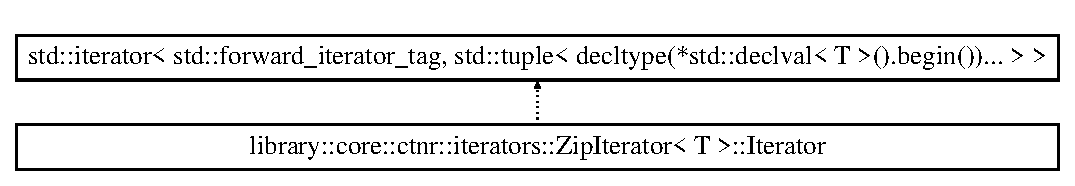
\includegraphics[height=2.000000cm]{classlibrary_1_1core_1_1ctnr_1_1iterators_1_1_zip_iterator_1_1_iterator}
\end{center}
\end{figure}
\subsection*{Public Member Functions}
\begin{DoxyCompactItemize}
\item 
\mbox{\hyperlink{classlibrary_1_1core_1_1ctnr_1_1iterators_1_1_zip_iterator_1_1_iterator_ab93e780bb41bdb0fbce8e852138051a4}{Iterator}} (decltype(\mbox{\hyperlink{classlibrary_1_1core_1_1ctnr_1_1iterators_1_1_zip_iterator_1_1_iterator_a37c838a652996c4a8d140f1cc3804e4a}{iterators\+\_\+}}) an\+Iterator\+List)
\item 
\mbox{\hyperlink{classlibrary_1_1core_1_1ctnr_1_1iterators_1_1_zip_iterator_1_1_iterator}{Iterator}} \& \mbox{\hyperlink{classlibrary_1_1core_1_1ctnr_1_1iterators_1_1_zip_iterator_1_1_iterator_ab41c609c9afe7e62fe6e4cceaa709771}{operator++}} ()
\item 
\mbox{\hyperlink{classlibrary_1_1core_1_1ctnr_1_1iterators_1_1_zip_iterator_1_1_iterator}{Iterator}} \mbox{\hyperlink{classlibrary_1_1core_1_1ctnr_1_1iterators_1_1_zip_iterator_1_1_iterator_abd2db3105f0aeedec986c6db965ba16f}{operator++}} (int)
\item 
bool \mbox{\hyperlink{classlibrary_1_1core_1_1ctnr_1_1iterators_1_1_zip_iterator_1_1_iterator_ae3e898d5e9a5f0aa7f1f076de6af8063}{operator!=}} (const \mbox{\hyperlink{classlibrary_1_1core_1_1ctnr_1_1iterators_1_1_zip_iterator_1_1_iterator}{Iterator}} \&an\+Iterator) const
\item 
auto \mbox{\hyperlink{classlibrary_1_1core_1_1ctnr_1_1iterators_1_1_zip_iterator_1_1_iterator_a34082110fb060868a9e15bc1b5c475a1}{operator$\ast$}} () const
\end{DoxyCompactItemize}
\subsection*{Public Attributes}
\begin{DoxyCompactItemize}
\item 
std\+::tuple$<$ decltype(std\+::declval$<$ T $>$).\mbox{\hyperlink{classlibrary_1_1core_1_1ctnr_1_1iterators_1_1_zip_iterator_a0467e25b565ac7b73b22a7002b87d189}{begin}}())... $>$ \mbox{\hyperlink{classlibrary_1_1core_1_1ctnr_1_1iterators_1_1_zip_iterator_1_1_iterator_a37c838a652996c4a8d140f1cc3804e4a}{iterators\+\_\+}}
\end{DoxyCompactItemize}


\subsection{Constructor \& Destructor Documentation}
\mbox{\Hypertarget{classlibrary_1_1core_1_1ctnr_1_1iterators_1_1_zip_iterator_1_1_iterator_ab93e780bb41bdb0fbce8e852138051a4}\label{classlibrary_1_1core_1_1ctnr_1_1iterators_1_1_zip_iterator_1_1_iterator_ab93e780bb41bdb0fbce8e852138051a4}} 
\index{library::core::ctnr::iterators::ZipIterator$<$ T $>$::Iterator@{library::core::ctnr::iterators::ZipIterator$<$ T $>$::Iterator}!Iterator@{Iterator}}
\index{Iterator@{Iterator}!library::core::ctnr::iterators::ZipIterator$<$ T $>$::Iterator@{library::core::ctnr::iterators::ZipIterator$<$ T $>$::Iterator}}
\subsubsection{\texorpdfstring{Iterator()}{Iterator()}}
{\footnotesize\ttfamily template$<$typename... T$>$ \\
\mbox{\hyperlink{classlibrary_1_1core_1_1ctnr_1_1iterators_1_1_zip_iterator}{library\+::core\+::ctnr\+::iterators\+::\+Zip\+Iterator}}$<$ T $>$\+::Iterator\+::\+Iterator (\begin{DoxyParamCaption}\item[{decltype(\mbox{\hyperlink{classlibrary_1_1core_1_1ctnr_1_1iterators_1_1_zip_iterator_1_1_iterator_a37c838a652996c4a8d140f1cc3804e4a}{iterators\+\_\+}})}]{an\+Iterator\+List }\end{DoxyParamCaption})\hspace{0.3cm}{\ttfamily [inline]}, {\ttfamily [explicit]}}



\subsection{Member Function Documentation}
\mbox{\Hypertarget{classlibrary_1_1core_1_1ctnr_1_1iterators_1_1_zip_iterator_1_1_iterator_ae3e898d5e9a5f0aa7f1f076de6af8063}\label{classlibrary_1_1core_1_1ctnr_1_1iterators_1_1_zip_iterator_1_1_iterator_ae3e898d5e9a5f0aa7f1f076de6af8063}} 
\index{library::core::ctnr::iterators::ZipIterator$<$ T $>$::Iterator@{library::core::ctnr::iterators::ZipIterator$<$ T $>$::Iterator}!operator"!=@{operator"!=}}
\index{operator"!=@{operator"!=}!library::core::ctnr::iterators::ZipIterator$<$ T $>$::Iterator@{library::core::ctnr::iterators::ZipIterator$<$ T $>$::Iterator}}
\subsubsection{\texorpdfstring{operator"!=()}{operator!=()}}
{\footnotesize\ttfamily template$<$typename... T$>$ \\
bool \mbox{\hyperlink{classlibrary_1_1core_1_1ctnr_1_1iterators_1_1_zip_iterator}{library\+::core\+::ctnr\+::iterators\+::\+Zip\+Iterator}}$<$ T $>$\+::Iterator\+::operator!= (\begin{DoxyParamCaption}\item[{const \mbox{\hyperlink{classlibrary_1_1core_1_1ctnr_1_1iterators_1_1_zip_iterator_1_1_iterator}{Iterator}} \&}]{an\+Iterator }\end{DoxyParamCaption}) const\hspace{0.3cm}{\ttfamily [inline]}}

\mbox{\Hypertarget{classlibrary_1_1core_1_1ctnr_1_1iterators_1_1_zip_iterator_1_1_iterator_a34082110fb060868a9e15bc1b5c475a1}\label{classlibrary_1_1core_1_1ctnr_1_1iterators_1_1_zip_iterator_1_1_iterator_a34082110fb060868a9e15bc1b5c475a1}} 
\index{library::core::ctnr::iterators::ZipIterator$<$ T $>$::Iterator@{library::core::ctnr::iterators::ZipIterator$<$ T $>$::Iterator}!operator$\ast$@{operator$\ast$}}
\index{operator$\ast$@{operator$\ast$}!library::core::ctnr::iterators::ZipIterator$<$ T $>$::Iterator@{library::core::ctnr::iterators::ZipIterator$<$ T $>$::Iterator}}
\subsubsection{\texorpdfstring{operator$\ast$()}{operator*()}}
{\footnotesize\ttfamily template$<$typename... T$>$ \\
auto \mbox{\hyperlink{classlibrary_1_1core_1_1ctnr_1_1iterators_1_1_zip_iterator}{library\+::core\+::ctnr\+::iterators\+::\+Zip\+Iterator}}$<$ T $>$\+::Iterator\+::operator$\ast$ (\begin{DoxyParamCaption}{ }\end{DoxyParamCaption}) const\hspace{0.3cm}{\ttfamily [inline]}}

\mbox{\Hypertarget{classlibrary_1_1core_1_1ctnr_1_1iterators_1_1_zip_iterator_1_1_iterator_ab41c609c9afe7e62fe6e4cceaa709771}\label{classlibrary_1_1core_1_1ctnr_1_1iterators_1_1_zip_iterator_1_1_iterator_ab41c609c9afe7e62fe6e4cceaa709771}} 
\index{library::core::ctnr::iterators::ZipIterator$<$ T $>$::Iterator@{library::core::ctnr::iterators::ZipIterator$<$ T $>$::Iterator}!operator++@{operator++}}
\index{operator++@{operator++}!library::core::ctnr::iterators::ZipIterator$<$ T $>$::Iterator@{library::core::ctnr::iterators::ZipIterator$<$ T $>$::Iterator}}
\subsubsection{\texorpdfstring{operator++()}{operator++()}\hspace{0.1cm}{\footnotesize\ttfamily [1/2]}}
{\footnotesize\ttfamily template$<$typename... T$>$ \\
\mbox{\hyperlink{classlibrary_1_1core_1_1ctnr_1_1iterators_1_1_zip_iterator_1_1_iterator}{Iterator}}\& \mbox{\hyperlink{classlibrary_1_1core_1_1ctnr_1_1iterators_1_1_zip_iterator}{library\+::core\+::ctnr\+::iterators\+::\+Zip\+Iterator}}$<$ T $>$\+::Iterator\+::operator++ (\begin{DoxyParamCaption}{ }\end{DoxyParamCaption})\hspace{0.3cm}{\ttfamily [inline]}}

\mbox{\Hypertarget{classlibrary_1_1core_1_1ctnr_1_1iterators_1_1_zip_iterator_1_1_iterator_abd2db3105f0aeedec986c6db965ba16f}\label{classlibrary_1_1core_1_1ctnr_1_1iterators_1_1_zip_iterator_1_1_iterator_abd2db3105f0aeedec986c6db965ba16f}} 
\index{library::core::ctnr::iterators::ZipIterator$<$ T $>$::Iterator@{library::core::ctnr::iterators::ZipIterator$<$ T $>$::Iterator}!operator++@{operator++}}
\index{operator++@{operator++}!library::core::ctnr::iterators::ZipIterator$<$ T $>$::Iterator@{library::core::ctnr::iterators::ZipIterator$<$ T $>$::Iterator}}
\subsubsection{\texorpdfstring{operator++()}{operator++()}\hspace{0.1cm}{\footnotesize\ttfamily [2/2]}}
{\footnotesize\ttfamily template$<$typename... T$>$ \\
\mbox{\hyperlink{classlibrary_1_1core_1_1ctnr_1_1iterators_1_1_zip_iterator_1_1_iterator}{Iterator}} \mbox{\hyperlink{classlibrary_1_1core_1_1ctnr_1_1iterators_1_1_zip_iterator}{library\+::core\+::ctnr\+::iterators\+::\+Zip\+Iterator}}$<$ T $>$\+::Iterator\+::operator++ (\begin{DoxyParamCaption}\item[{int}]{ }\end{DoxyParamCaption})\hspace{0.3cm}{\ttfamily [inline]}}



\subsection{Member Data Documentation}
\mbox{\Hypertarget{classlibrary_1_1core_1_1ctnr_1_1iterators_1_1_zip_iterator_1_1_iterator_a37c838a652996c4a8d140f1cc3804e4a}\label{classlibrary_1_1core_1_1ctnr_1_1iterators_1_1_zip_iterator_1_1_iterator_a37c838a652996c4a8d140f1cc3804e4a}} 
\index{library::core::ctnr::iterators::ZipIterator$<$ T $>$::Iterator@{library::core::ctnr::iterators::ZipIterator$<$ T $>$::Iterator}!iterators\_@{iterators\_}}
\index{iterators\_@{iterators\_}!library::core::ctnr::iterators::ZipIterator$<$ T $>$::Iterator@{library::core::ctnr::iterators::ZipIterator$<$ T $>$::Iterator}}
\subsubsection{\texorpdfstring{iterators\_}{iterators\_}}
{\footnotesize\ttfamily template$<$typename... T$>$ \\
std\+::tuple$<$decltype(std\+::declval$<$T$>$).\mbox{\hyperlink{classlibrary_1_1core_1_1ctnr_1_1iterators_1_1_zip_iterator_a0467e25b565ac7b73b22a7002b87d189}{begin}}())...$>$ \mbox{\hyperlink{classlibrary_1_1core_1_1ctnr_1_1iterators_1_1_zip_iterator}{library\+::core\+::ctnr\+::iterators\+::\+Zip\+Iterator}}$<$ T $>$\+::Iterator\+::iterators\+\_\+}



The documentation for this class was generated from the following file\+:\begin{DoxyCompactItemize}
\item 
include/\+Library/\+Core/\+Containers/\+Iterators/\mbox{\hyperlink{_zip_8hpp}{Zip.\+hpp}}\end{DoxyCompactItemize}

\hypertarget{classlibrary_1_1core_1_1ctnr_1_1_dictionary_1_1_iterator}{}\section{library\+:\+:core\+:\+:ctnr\+:\+:Dictionary\+:\+:Iterator Class Reference}
\label{classlibrary_1_1core_1_1ctnr_1_1_dictionary_1_1_iterator}\index{library\+::core\+::ctnr\+::\+Dictionary\+::\+Iterator@{library\+::core\+::ctnr\+::\+Dictionary\+::\+Iterator}}
\subsection*{Public Types}
\begin{DoxyCompactItemize}
\item 
\mbox{\Hypertarget{classlibrary_1_1core_1_1ctnr_1_1_dictionary_1_1_iterator_a990205e908ac1bafcd754993219b805e}\label{classlibrary_1_1core_1_1ctnr_1_1_dictionary_1_1_iterator_a990205e908ac1bafcd754993219b805e}} 
typedef \hyperlink{_ordered_map_8hpp_a1c0809231c3bc9fccce602bd7941a36b}{Ordered\+Map}$<$ \hyperlink{classlibrary_1_1core_1_1types_1_1_string}{Dictionary\+::\+Key}, \hyperlink{classlibrary_1_1core_1_1ctnr_1_1_object}{Dictionary\+::\+Value} $>$\+::iterator {\bfseries Map\+Iterator}
\end{DoxyCompactItemize}
\subsection*{Public Member Functions}
\begin{DoxyCompactItemize}
\item 
\mbox{\Hypertarget{classlibrary_1_1core_1_1ctnr_1_1_dictionary_1_1_iterator_aa490a8fff909725ad18d1cb4f836fa3f}\label{classlibrary_1_1core_1_1ctnr_1_1_dictionary_1_1_iterator_aa490a8fff909725ad18d1cb4f836fa3f}} 
{\bfseries Iterator} (const Iterator\+::\+Map\+Iterator \&an\+Ordered\+Map\+It)
\item 
\mbox{\Hypertarget{classlibrary_1_1core_1_1ctnr_1_1_dictionary_1_1_iterator_af67d8a90f351b6edd60c4e08b1210d0f}\label{classlibrary_1_1core_1_1ctnr_1_1_dictionary_1_1_iterator_af67d8a90f351b6edd60c4e08b1210d0f}} 
{\bfseries Iterator} (const \hyperlink{classlibrary_1_1core_1_1ctnr_1_1_dictionary_1_1_iterator}{Iterator} \&a\+Iterator)
\item 
\mbox{\Hypertarget{classlibrary_1_1core_1_1ctnr_1_1_dictionary_1_1_iterator_a194c16d77f2f2d37e1ae2a5b55165520}\label{classlibrary_1_1core_1_1ctnr_1_1_dictionary_1_1_iterator_a194c16d77f2f2d37e1ae2a5b55165520}} 
\hyperlink{classlibrary_1_1core_1_1ctnr_1_1_dictionary_1_1_iterator}{Iterator} \& {\bfseries operator=} (const \hyperlink{classlibrary_1_1core_1_1ctnr_1_1_dictionary_1_1_iterator}{Iterator} \&a\+Iterator)
\item 
\mbox{\Hypertarget{classlibrary_1_1core_1_1ctnr_1_1_dictionary_1_1_iterator_a4901ad2232bec38f673c7442b8460c93}\label{classlibrary_1_1core_1_1ctnr_1_1_dictionary_1_1_iterator_a4901ad2232bec38f673c7442b8460c93}} 
bool {\bfseries operator==} (const \hyperlink{classlibrary_1_1core_1_1ctnr_1_1_dictionary_1_1_iterator}{Iterator} \&a\+Iterator) const
\item 
\mbox{\Hypertarget{classlibrary_1_1core_1_1ctnr_1_1_dictionary_1_1_iterator_ae8cd94a904fb59137a17b7b220bce384}\label{classlibrary_1_1core_1_1ctnr_1_1_dictionary_1_1_iterator_ae8cd94a904fb59137a17b7b220bce384}} 
bool {\bfseries operator!=} (const \hyperlink{classlibrary_1_1core_1_1ctnr_1_1_dictionary_1_1_iterator}{Iterator} \&a\+Iterator) const
\item 
\mbox{\Hypertarget{classlibrary_1_1core_1_1ctnr_1_1_dictionary_1_1_iterator_ab162ab9f80c90a75c30d5c23b4343f11}\label{classlibrary_1_1core_1_1ctnr_1_1_dictionary_1_1_iterator_ab162ab9f80c90a75c30d5c23b4343f11}} 
const \hyperlink{classlibrary_1_1core_1_1ctnr_1_1_dictionary_1_1_iterator}{Iterator} \& {\bfseries operator$\ast$} () const
\item 
\mbox{\Hypertarget{classlibrary_1_1core_1_1ctnr_1_1_dictionary_1_1_iterator_ab0d2327725731d62770ae87f3b5b6003}\label{classlibrary_1_1core_1_1ctnr_1_1_dictionary_1_1_iterator_ab0d2327725731d62770ae87f3b5b6003}} 
const \hyperlink{classlibrary_1_1core_1_1ctnr_1_1_dictionary_1_1_iterator}{Iterator} $\ast$ {\bfseries operator-\/$>$} () const
\item 
\mbox{\Hypertarget{classlibrary_1_1core_1_1ctnr_1_1_dictionary_1_1_iterator_a948d120f6e384f2567a000f356ff80b7}\label{classlibrary_1_1core_1_1ctnr_1_1_dictionary_1_1_iterator_a948d120f6e384f2567a000f356ff80b7}} 
\hyperlink{classlibrary_1_1core_1_1ctnr_1_1_dictionary_1_1_iterator}{Iterator} \& {\bfseries operator$\ast$} ()
\item 
\mbox{\Hypertarget{classlibrary_1_1core_1_1ctnr_1_1_dictionary_1_1_iterator_ad1a9208897733e9e22fdf9ea3248acc6}\label{classlibrary_1_1core_1_1ctnr_1_1_dictionary_1_1_iterator_ad1a9208897733e9e22fdf9ea3248acc6}} 
\hyperlink{classlibrary_1_1core_1_1ctnr_1_1_dictionary_1_1_iterator}{Iterator} $\ast$ {\bfseries operator-\/$>$} ()
\item 
\mbox{\Hypertarget{classlibrary_1_1core_1_1ctnr_1_1_dictionary_1_1_iterator_a89151ad07a4b475b62673fd933535714}\label{classlibrary_1_1core_1_1ctnr_1_1_dictionary_1_1_iterator_a89151ad07a4b475b62673fd933535714}} 
\hyperlink{classlibrary_1_1core_1_1ctnr_1_1_object}{Dictionary\+::\+Value} \& {\bfseries operator\mbox{[}$\,$\mbox{]}} (const \hyperlink{classlibrary_1_1core_1_1types_1_1_string}{Dictionary\+::\+Key} \&a\+Key)
\item 
\mbox{\Hypertarget{classlibrary_1_1core_1_1ctnr_1_1_dictionary_1_1_iterator_a535cdfc550d367249a109790a5f8e3e7}\label{classlibrary_1_1core_1_1ctnr_1_1_dictionary_1_1_iterator_a535cdfc550d367249a109790a5f8e3e7}} 
\hyperlink{classlibrary_1_1core_1_1ctnr_1_1_dictionary_1_1_iterator}{Iterator} \& {\bfseries operator++} ()
\item 
\mbox{\Hypertarget{classlibrary_1_1core_1_1ctnr_1_1_dictionary_1_1_iterator_a51ddd344a01b04f1ac8938a3019ec92a}\label{classlibrary_1_1core_1_1ctnr_1_1_dictionary_1_1_iterator_a51ddd344a01b04f1ac8938a3019ec92a}} 
\hyperlink{classlibrary_1_1core_1_1ctnr_1_1_dictionary_1_1_iterator}{Iterator} {\bfseries operator++} (int)
\item 
\mbox{\Hypertarget{classlibrary_1_1core_1_1ctnr_1_1_dictionary_1_1_iterator_a8400447d918135a36993d445fe2259b7}\label{classlibrary_1_1core_1_1ctnr_1_1_dictionary_1_1_iterator_a8400447d918135a36993d445fe2259b7}} 
\hyperlink{classlibrary_1_1core_1_1ctnr_1_1_dictionary_1_1_iterator}{Iterator} \& {\bfseries operator-\/-\/} ()
\item 
\mbox{\Hypertarget{classlibrary_1_1core_1_1ctnr_1_1_dictionary_1_1_iterator_a0e6049d9ccc80f1b0775cd5a3aff1983}\label{classlibrary_1_1core_1_1ctnr_1_1_dictionary_1_1_iterator_a0e6049d9ccc80f1b0775cd5a3aff1983}} 
\hyperlink{classlibrary_1_1core_1_1ctnr_1_1_dictionary_1_1_iterator}{Iterator} {\bfseries operator-\/-\/} (int)
\item 
\mbox{\Hypertarget{classlibrary_1_1core_1_1ctnr_1_1_dictionary_1_1_iterator_aa2d6a49d852730a914282aacbab8462d}\label{classlibrary_1_1core_1_1ctnr_1_1_dictionary_1_1_iterator_aa2d6a49d852730a914282aacbab8462d}} 
const \hyperlink{classlibrary_1_1core_1_1types_1_1_string}{Dictionary\+::\+Key} \& {\bfseries access\+Key} () const
\item 
\mbox{\Hypertarget{classlibrary_1_1core_1_1ctnr_1_1_dictionary_1_1_iterator_af81ea86e2febbe6ca73e502987de33a1}\label{classlibrary_1_1core_1_1ctnr_1_1_dictionary_1_1_iterator_af81ea86e2febbe6ca73e502987de33a1}} 
const \hyperlink{classlibrary_1_1core_1_1ctnr_1_1_object}{Dictionary\+::\+Value} \& {\bfseries access\+Value} () const
\item 
\mbox{\Hypertarget{classlibrary_1_1core_1_1ctnr_1_1_dictionary_1_1_iterator_a7ef51bee5765a7b2464121552ac2ecfe}\label{classlibrary_1_1core_1_1ctnr_1_1_dictionary_1_1_iterator_a7ef51bee5765a7b2464121552ac2ecfe}} 
\hyperlink{classlibrary_1_1core_1_1ctnr_1_1_object}{Dictionary\+::\+Value} \& {\bfseries access\+Value} ()
\item 
\mbox{\Hypertarget{classlibrary_1_1core_1_1ctnr_1_1_dictionary_1_1_iterator_a202f6a93a302e94078a33c1bcc999deb}\label{classlibrary_1_1core_1_1ctnr_1_1_dictionary_1_1_iterator_a202f6a93a302e94078a33c1bcc999deb}} 
const Iterator\+::\+Map\+Iterator \& {\bfseries access\+Map\+Iterator} () const
\item 
\mbox{\Hypertarget{classlibrary_1_1core_1_1ctnr_1_1_dictionary_1_1_iterator_acbc6831522ba983453d99696b58e055c}\label{classlibrary_1_1core_1_1ctnr_1_1_dictionary_1_1_iterator_acbc6831522ba983453d99696b58e055c}} 
Iterator\+::\+Map\+Iterator \& {\bfseries access\+Map\+Iterator} ()
\end{DoxyCompactItemize}


The documentation for this class was generated from the following file\+:\begin{DoxyCompactItemize}
\item 
include/\+Library/\+Core/\+Containers/\hyperlink{_dictionary_8hpp}{Dictionary.\+hpp}\end{DoxyCompactItemize}

\hypertarget{classlibrary_1_1core_1_1utils_1_1_print_1_1_line_buffer}{}\section{library\+:\+:core\+:\+:utils\+:\+:Print\+:\+:Line\+Buffer Class Reference}
\label{classlibrary_1_1core_1_1utils_1_1_print_1_1_line_buffer}\index{library\+::core\+::utils\+::\+Print\+::\+Line\+Buffer@{library\+::core\+::utils\+::\+Print\+::\+Line\+Buffer}}


{\ttfamily \#include $<$Print.\+hpp$>$}

\subsection*{Public Member Functions}
\begin{DoxyCompactItemize}
\item 
\hyperlink{classlibrary_1_1core_1_1utils_1_1_print_1_1_line_buffer_a241c89010e599cd15025fdaa240c66f8}{Line\+Buffer} (std\+::ostream \&an\+Output\+Stream, uint an\+Indentation)
\item 
\hyperlink{classlibrary_1_1core_1_1utils_1_1_print_1_1_line_buffer_afc353daf14e3a1f76f6d7b73907e3bbe}{Line\+Buffer} (const \hyperlink{classlibrary_1_1core_1_1utils_1_1_print_1_1_line_buffer}{Line\+Buffer} \&a\+Line\+Buffer)=delete
\item 
\hyperlink{classlibrary_1_1core_1_1utils_1_1_print_1_1_line_buffer_a45f71ed47bf91cb76c31135e04a60a7b}{Line\+Buffer} (\hyperlink{classlibrary_1_1core_1_1utils_1_1_print_1_1_line_buffer}{Line\+Buffer} \&\&a\+Line\+Buffer)=default
\item 
\hyperlink{classlibrary_1_1core_1_1utils_1_1_print_1_1_line_buffer_aed429cbff736a609eeb1b87c984006ac}{$\sim$\+Line\+Buffer} ()
\item 
{\footnotesize template$<$class T $>$ }\\\hyperlink{classlibrary_1_1core_1_1utils_1_1_print_1_1_line_buffer}{Line\+Buffer} \& \hyperlink{classlibrary_1_1core_1_1utils_1_1_print_1_1_line_buffer_aceff405c94de38866120abc55093762f}{operator$<$$<$} (const T \&an\+Object)
\end{DoxyCompactItemize}


\subsection{Constructor \& Destructor Documentation}
\mbox{\Hypertarget{classlibrary_1_1core_1_1utils_1_1_print_1_1_line_buffer_a241c89010e599cd15025fdaa240c66f8}\label{classlibrary_1_1core_1_1utils_1_1_print_1_1_line_buffer_a241c89010e599cd15025fdaa240c66f8}} 
\index{library\+::core\+::utils\+::\+Print\+::\+Line\+Buffer@{library\+::core\+::utils\+::\+Print\+::\+Line\+Buffer}!Line\+Buffer@{Line\+Buffer}}
\index{Line\+Buffer@{Line\+Buffer}!library\+::core\+::utils\+::\+Print\+::\+Line\+Buffer@{library\+::core\+::utils\+::\+Print\+::\+Line\+Buffer}}
\subsubsection{\texorpdfstring{Line\+Buffer()}{LineBuffer()}\hspace{0.1cm}{\footnotesize\ttfamily [1/3]}}
{\footnotesize\ttfamily library\+::core\+::utils\+::\+Print\+::\+Line\+Buffer\+::\+Line\+Buffer (\begin{DoxyParamCaption}\item[{std\+::ostream \&}]{an\+Output\+Stream,  }\item[{uint}]{an\+Indentation }\end{DoxyParamCaption})}

\mbox{\Hypertarget{classlibrary_1_1core_1_1utils_1_1_print_1_1_line_buffer_afc353daf14e3a1f76f6d7b73907e3bbe}\label{classlibrary_1_1core_1_1utils_1_1_print_1_1_line_buffer_afc353daf14e3a1f76f6d7b73907e3bbe}} 
\index{library\+::core\+::utils\+::\+Print\+::\+Line\+Buffer@{library\+::core\+::utils\+::\+Print\+::\+Line\+Buffer}!Line\+Buffer@{Line\+Buffer}}
\index{Line\+Buffer@{Line\+Buffer}!library\+::core\+::utils\+::\+Print\+::\+Line\+Buffer@{library\+::core\+::utils\+::\+Print\+::\+Line\+Buffer}}
\subsubsection{\texorpdfstring{Line\+Buffer()}{LineBuffer()}\hspace{0.1cm}{\footnotesize\ttfamily [2/3]}}
{\footnotesize\ttfamily library\+::core\+::utils\+::\+Print\+::\+Line\+Buffer\+::\+Line\+Buffer (\begin{DoxyParamCaption}\item[{const \hyperlink{classlibrary_1_1core_1_1utils_1_1_print_1_1_line_buffer}{Line\+Buffer} \&}]{a\+Line\+Buffer }\end{DoxyParamCaption})\hspace{0.3cm}{\ttfamily [delete]}}

\mbox{\Hypertarget{classlibrary_1_1core_1_1utils_1_1_print_1_1_line_buffer_a45f71ed47bf91cb76c31135e04a60a7b}\label{classlibrary_1_1core_1_1utils_1_1_print_1_1_line_buffer_a45f71ed47bf91cb76c31135e04a60a7b}} 
\index{library\+::core\+::utils\+::\+Print\+::\+Line\+Buffer@{library\+::core\+::utils\+::\+Print\+::\+Line\+Buffer}!Line\+Buffer@{Line\+Buffer}}
\index{Line\+Buffer@{Line\+Buffer}!library\+::core\+::utils\+::\+Print\+::\+Line\+Buffer@{library\+::core\+::utils\+::\+Print\+::\+Line\+Buffer}}
\subsubsection{\texorpdfstring{Line\+Buffer()}{LineBuffer()}\hspace{0.1cm}{\footnotesize\ttfamily [3/3]}}
{\footnotesize\ttfamily library\+::core\+::utils\+::\+Print\+::\+Line\+Buffer\+::\+Line\+Buffer (\begin{DoxyParamCaption}\item[{\hyperlink{classlibrary_1_1core_1_1utils_1_1_print_1_1_line_buffer}{Line\+Buffer} \&\&}]{a\+Line\+Buffer }\end{DoxyParamCaption})\hspace{0.3cm}{\ttfamily [default]}}

\mbox{\Hypertarget{classlibrary_1_1core_1_1utils_1_1_print_1_1_line_buffer_aed429cbff736a609eeb1b87c984006ac}\label{classlibrary_1_1core_1_1utils_1_1_print_1_1_line_buffer_aed429cbff736a609eeb1b87c984006ac}} 
\index{library\+::core\+::utils\+::\+Print\+::\+Line\+Buffer@{library\+::core\+::utils\+::\+Print\+::\+Line\+Buffer}!````~Line\+Buffer@{$\sim$\+Line\+Buffer}}
\index{````~Line\+Buffer@{$\sim$\+Line\+Buffer}!library\+::core\+::utils\+::\+Print\+::\+Line\+Buffer@{library\+::core\+::utils\+::\+Print\+::\+Line\+Buffer}}
\subsubsection{\texorpdfstring{$\sim$\+Line\+Buffer()}{~LineBuffer()}}
{\footnotesize\ttfamily library\+::core\+::utils\+::\+Print\+::\+Line\+Buffer\+::$\sim$\+Line\+Buffer (\begin{DoxyParamCaption}{ }\end{DoxyParamCaption})}



\subsection{Member Function Documentation}
\mbox{\Hypertarget{classlibrary_1_1core_1_1utils_1_1_print_1_1_line_buffer_aceff405c94de38866120abc55093762f}\label{classlibrary_1_1core_1_1utils_1_1_print_1_1_line_buffer_aceff405c94de38866120abc55093762f}} 
\index{library\+::core\+::utils\+::\+Print\+::\+Line\+Buffer@{library\+::core\+::utils\+::\+Print\+::\+Line\+Buffer}!operator$<$$<$@{operator$<$$<$}}
\index{operator$<$$<$@{operator$<$$<$}!library\+::core\+::utils\+::\+Print\+::\+Line\+Buffer@{library\+::core\+::utils\+::\+Print\+::\+Line\+Buffer}}
\subsubsection{\texorpdfstring{operator$<$$<$()}{operator<<()}}
{\footnotesize\ttfamily template$<$class T $>$ \\
\hyperlink{classlibrary_1_1core_1_1utils_1_1_print_1_1_line_buffer}{Line\+Buffer}\& library\+::core\+::utils\+::\+Print\+::\+Line\+Buffer\+::operator$<$$<$ (\begin{DoxyParamCaption}\item[{const T \&}]{an\+Object }\end{DoxyParamCaption})\hspace{0.3cm}{\ttfamily [inline]}}



The documentation for this class was generated from the following files\+:\begin{DoxyCompactItemize}
\item 
include/\+Library/\+Core/\+Utilities/\hyperlink{_print_8hpp}{Print.\+hpp}\item 
src/\+Library/\+Core/\+Utilities/\hyperlink{_print_8cpp}{Print.\+cpp}\end{DoxyCompactItemize}

\hypertarget{classlibrary_1_1core_1_1_logger}{}\section{library\+:\+:core\+:\+:Logger Class Reference}
\label{classlibrary_1_1core_1_1_logger}\index{library\+::core\+::\+Logger@{library\+::core\+::\+Logger}}


Log management.  




{\ttfamily \#include $<$Logger.\+hpp$>$}

\subsection*{Public Member Functions}
\begin{DoxyCompactItemize}
\item 
\mbox{\Hypertarget{classlibrary_1_1core_1_1_logger_a0bc89b6aca42f5c7f08df824be5a8f2b}\label{classlibrary_1_1core_1_1_logger_a0bc89b6aca42f5c7f08df824be5a8f2b}} 
{\bfseries Logger} (const \hyperlink{classlibrary_1_1core_1_1types_1_1_string}{String} \&a\+Channel)
\item 
\mbox{\Hypertarget{classlibrary_1_1core_1_1_logger_aca8b3f76a6c88286ff0521d2dccfc86e}\label{classlibrary_1_1core_1_1_logger_aca8b3f76a6c88286ff0521d2dccfc86e}} 
\hyperlink{classlibrary_1_1core_1_1logger_1_1_pump}{Pump} {\bfseries operator()} (const Severity \&a\+Severity, const \hyperlink{classlibrary_1_1core_1_1types_1_1_integer}{Integer} \&a\+Line, const \hyperlink{classlibrary_1_1core_1_1types_1_1_string}{String} \&a\+File, const \hyperlink{classlibrary_1_1core_1_1types_1_1_string}{String} \&a\+Function)
\item 
\mbox{\Hypertarget{classlibrary_1_1core_1_1_logger_ae0bdb3a8d52dd8f7d359757d821ccfef}\label{classlibrary_1_1core_1_1_logger_ae0bdb3a8d52dd8f7d359757d821ccfef}} 
{\footnotesize template$<$class T $>$ }\\\hyperlink{classlibrary_1_1core_1_1logger_1_1_pump}{Pump} {\bfseries operator$<$$<$} (const T \&an\+Object)
\item 
\mbox{\Hypertarget{classlibrary_1_1core_1_1_logger_a61b860f2a6b4c54accdb04d7b15e3653}\label{classlibrary_1_1core_1_1_logger_a61b860f2a6b4c54accdb04d7b15e3653}} 
\hyperlink{classlibrary_1_1core_1_1types_1_1_string}{String} {\bfseries get\+Channel} () const
\end{DoxyCompactItemize}
\subsection*{Static Public Member Functions}
\begin{DoxyCompactItemize}
\item 
\mbox{\Hypertarget{classlibrary_1_1core_1_1_logger_a2f0a86c1a3237b8023efdbc3727dbb5a}\label{classlibrary_1_1core_1_1_logger_a2f0a86c1a3237b8023efdbc3727dbb5a}} 
static \hyperlink{classlibrary_1_1core_1_1_logger}{Logger} {\bfseries Console} (const Severity \&a\+Severity)
\item 
\mbox{\Hypertarget{classlibrary_1_1core_1_1_logger_a07e56c9a149007c30220eb9538e3b273}\label{classlibrary_1_1core_1_1_logger_a07e56c9a149007c30220eb9538e3b273}} 
static \hyperlink{classlibrary_1_1core_1_1_logger}{Logger} {\bfseries Console} (const \hyperlink{classlibrary_1_1core_1_1types_1_1_string}{String} \&a\+Channel, const Severity \&a\+Severity)
\item 
\mbox{\Hypertarget{classlibrary_1_1core_1_1_logger_a0b20a0248c34a111c7a18043185586ff}\label{classlibrary_1_1core_1_1_logger_a0b20a0248c34a111c7a18043185586ff}} 
static \hyperlink{classlibrary_1_1core_1_1_logger}{Logger} \& {\bfseries Global} ()
\end{DoxyCompactItemize}


\subsection{Detailed Description}
Log management. 

The documentation for this class was generated from the following file\+:\begin{DoxyCompactItemize}
\item 
include/\+Library/\+Core/\hyperlink{_logger_8hpp}{Logger.\+hpp}\end{DoxyCompactItemize}

\hypertarget{classlibrary_1_1core_1_1ctnr_1_1_object}{}\section{library\+:\+:core\+:\+:ctnr\+:\+:Object Class Reference}
\label{classlibrary_1_1core_1_1ctnr_1_1_object}\index{library\+::core\+::ctnr\+::\+Object@{library\+::core\+::ctnr\+::\+Object}}


Universal type container.  




{\ttfamily \#include $<$Object.\+hpp$>$}

\subsection*{Public Types}
\begin{DoxyCompactItemize}
\item 
enum \hyperlink{classlibrary_1_1core_1_1ctnr_1_1_object_a0766006ad111133d70349019551b31d6}{Type} \{ \newline
\hyperlink{classlibrary_1_1core_1_1ctnr_1_1_object_a0766006ad111133d70349019551b31d6aec0fc0100c4fc1ce4eea230c3dc10360}{Type\+::\+Undefined}, 
\hyperlink{classlibrary_1_1core_1_1ctnr_1_1_object_a0766006ad111133d70349019551b31d6a27226c864bac7454a8504f8edb15d95b}{Type\+::\+Boolean}, 
\hyperlink{classlibrary_1_1core_1_1ctnr_1_1_object_a0766006ad111133d70349019551b31d6aa0faef0851b4294c06f2b94bb1cb2044}{Type\+::\+Integer}, 
\hyperlink{classlibrary_1_1core_1_1ctnr_1_1_object_a0766006ad111133d70349019551b31d6a7f80fcc452c2f1ed2bb51b39d0864df1}{Type\+::\+Real}, 
\newline
\hyperlink{classlibrary_1_1core_1_1ctnr_1_1_object_a0766006ad111133d70349019551b31d6a27118326006d3829667a400ad23d5d98}{Type\+::\+String}, 
\hyperlink{classlibrary_1_1core_1_1ctnr_1_1_object_a0766006ad111133d70349019551b31d6a3beb75d1563ebc22253341be4ce57f44}{Type\+::\+Dictionary}, 
\hyperlink{classlibrary_1_1core_1_1ctnr_1_1_object_a0766006ad111133d70349019551b31d6a4410ec34d9e6c1a68100ca0ce033fb17}{Type\+::\+Array}
 \}
\item 
enum \hyperlink{classlibrary_1_1core_1_1ctnr_1_1_object_a7bf8961c4ef65f691aa2993ec405c647}{Format} \{ \hyperlink{classlibrary_1_1core_1_1ctnr_1_1_object_a7bf8961c4ef65f691aa2993ec405c647aec0fc0100c4fc1ce4eea230c3dc10360}{Format\+::\+Undefined}, 
\hyperlink{classlibrary_1_1core_1_1ctnr_1_1_object_a7bf8961c4ef65f691aa2993ec405c647a0ecd11c1d7a287401d148a23bbd7a2f8}{Format\+::\+J\+S\+ON}
 \}
\end{DoxyCompactItemize}
\subsection*{Public Member Functions}
\begin{DoxyCompactItemize}
\item 
\hyperlink{classlibrary_1_1core_1_1ctnr_1_1_object_a51bb72dec3a1b2738e0ad92b977b8d8d}{Object} ()=delete
\begin{DoxyCompactList}\small\item\em Default constructor (disabled) \end{DoxyCompactList}\item 
\hyperlink{classlibrary_1_1core_1_1ctnr_1_1_object_a351131c4c1d6d7bd4f488ba99d7bf2d5}{Object} (std\+::initializer\+\_\+list$<$ \hyperlink{namespacelibrary_1_1core_1_1ctnr_aad6f8de4c0f279c10436d59d4ace74bd}{ctnr\+::\+Pair}$<$ \hyperlink{classlibrary_1_1core_1_1types_1_1_string}{types\+::\+String}, \hyperlink{classlibrary_1_1core_1_1ctnr_1_1_object}{Object} $>$$>$ a\+List)
\begin{DoxyCompactList}\small\item\em Constructs an object using an initializer list. \end{DoxyCompactList}\item 
\hyperlink{classlibrary_1_1core_1_1ctnr_1_1_object_a90f9c4579306498a5da413ac89ac0109}{Object} (const \hyperlink{classlibrary_1_1core_1_1ctnr_1_1_object}{Object} \&an\+Object)
\begin{DoxyCompactList}\small\item\em Copy constructor. \end{DoxyCompactList}\item 
\hyperlink{classlibrary_1_1core_1_1ctnr_1_1_object_a18a5350937267e55df0a76f5ce154a7a}{$\sim$\+Object} ()
\begin{DoxyCompactList}\small\item\em Destructor. \end{DoxyCompactList}\item 
\hyperlink{classlibrary_1_1core_1_1ctnr_1_1_object}{Object} \& \hyperlink{classlibrary_1_1core_1_1ctnr_1_1_object_acbc5a6b4e2971d1cb977867d086832fe}{operator=} (const \hyperlink{classlibrary_1_1core_1_1ctnr_1_1_object}{Object} \&an\+Object)
\begin{DoxyCompactList}\small\item\em Assignment operator. \end{DoxyCompactList}\item 
bool \hyperlink{classlibrary_1_1core_1_1ctnr_1_1_object_a543801cb9c7c22432603aca5435595e9}{operator==} (const \hyperlink{classlibrary_1_1core_1_1ctnr_1_1_object}{Object} \&an\+Object) const
\begin{DoxyCompactList}\small\item\em Equal to operator. \end{DoxyCompactList}\item 
bool \hyperlink{classlibrary_1_1core_1_1ctnr_1_1_object_a8544bc0fbc6db8b12c8dabd51b075aa5}{operator!=} (const \hyperlink{classlibrary_1_1core_1_1ctnr_1_1_object}{Object} \&an\+Object) const
\begin{DoxyCompactList}\small\item\em Not equal to operator. \end{DoxyCompactList}\item 
const \hyperlink{classlibrary_1_1core_1_1ctnr_1_1_object}{Object} \& \hyperlink{classlibrary_1_1core_1_1ctnr_1_1_object_ad5b78e31dbe7d2cfddb14240b573862b}{operator\mbox{[}$\,$\mbox{]}} (const \hyperlink{classlibrary_1_1core_1_1types_1_1_string}{types\+::\+String} \&a\+Key) const
\item 
const \hyperlink{classlibrary_1_1core_1_1ctnr_1_1_object}{Object} \& \hyperlink{classlibrary_1_1core_1_1ctnr_1_1_object_a4f246b6d17dab0ebb1341fdb887064ad}{operator\mbox{[}$\,$\mbox{]}} (const \hyperlink{namespacelibrary_1_1core_1_1types_ad87eeb821d7067ec94e06ed1980d6350}{types\+::\+Index} \&an\+Index) const
\item 
\hyperlink{classlibrary_1_1core_1_1ctnr_1_1_object}{Object} \& \hyperlink{classlibrary_1_1core_1_1ctnr_1_1_object_ab5ef00d90b9b88c0dea26f38050a1224}{operator\mbox{[}$\,$\mbox{]}} (const \hyperlink{classlibrary_1_1core_1_1types_1_1_string}{types\+::\+String} \&a\+Key)
\item 
\hyperlink{classlibrary_1_1core_1_1ctnr_1_1_object}{Object} \& \hyperlink{classlibrary_1_1core_1_1ctnr_1_1_object_a20fbb0cb8c3f2eacbc9ae67999cb6a89}{operator\mbox{[}$\,$\mbox{]}} (const \hyperlink{namespacelibrary_1_1core_1_1types_ad87eeb821d7067ec94e06ed1980d6350}{types\+::\+Index} \&an\+Index)
\item 
bool \hyperlink{classlibrary_1_1core_1_1ctnr_1_1_object_af6d1f46d5ad8cd5b2440191f085dac2b}{is\+Defined} () const
\item 
bool \hyperlink{classlibrary_1_1core_1_1ctnr_1_1_object_a5a53a86979988ae7145277764cd70ca2}{is\+Boolean} () const
\item 
bool \hyperlink{classlibrary_1_1core_1_1ctnr_1_1_object_a13d9accc0093611957481eede274fb5d}{is\+Integer} () const
\item 
bool \hyperlink{classlibrary_1_1core_1_1ctnr_1_1_object_ab638356093a8b746f178fde641632d91}{is\+Real} () const
\item 
bool \hyperlink{classlibrary_1_1core_1_1ctnr_1_1_object_ae7248bcf0097fbd940dfa6a93097cd60}{is\+String} () const
\item 
bool \hyperlink{classlibrary_1_1core_1_1ctnr_1_1_object_a118fd5c5fc2768af41953ba7d4cde20e}{is\+Dictionary} () const
\item 
bool \hyperlink{classlibrary_1_1core_1_1ctnr_1_1_object_ab400e2c5b6516a9e69b3d0a7ac2178c5}{is\+Array} () const
\item 
const bool \& \hyperlink{classlibrary_1_1core_1_1ctnr_1_1_object_a0624bcf2292bb76848f3c284eb537d88}{access\+Boolean} () const
\item 
const \hyperlink{classlibrary_1_1core_1_1types_1_1_integer}{types\+::\+Integer} \& \hyperlink{classlibrary_1_1core_1_1ctnr_1_1_object_a0560b17f10faa200b8e180bcc11e6ab5}{access\+Integer} () const
\item 
const \hyperlink{classlibrary_1_1core_1_1types_1_1_real}{types\+::\+Real} \& \hyperlink{classlibrary_1_1core_1_1ctnr_1_1_object_a562d44d2e8bc8963b9da4591b6d94b32}{access\+Real} () const
\item 
const \hyperlink{classlibrary_1_1core_1_1types_1_1_string}{types\+::\+String} \& \hyperlink{classlibrary_1_1core_1_1ctnr_1_1_object_acdf93eb3e2d10c65ed7775f3d42cccb5}{access\+String} () const
\item 
const \hyperlink{classlibrary_1_1core_1_1ctnr_1_1_dictionary}{ctnr\+::\+Dictionary} \& \hyperlink{classlibrary_1_1core_1_1ctnr_1_1_object_ae0106ea013aa0f8ef23b9df01870f1af}{access\+Dictionary} () const
\item 
const \hyperlink{classlibrary_1_1core_1_1ctnr_1_1_array}{ctnr\+::\+Array}$<$ \hyperlink{classlibrary_1_1core_1_1ctnr_1_1_object}{Object} $>$ \& \hyperlink{classlibrary_1_1core_1_1ctnr_1_1_object_a09ef59cdf734b500ccab14933cf0b8d8}{access\+Array} () const
\item 
\hyperlink{classlibrary_1_1core_1_1ctnr_1_1_object_a0766006ad111133d70349019551b31d6}{Object\+::\+Type} \hyperlink{classlibrary_1_1core_1_1ctnr_1_1_object_aa2cc92ae24eb576e0f06af4dce8b7151}{get\+Type} () const
\item 
bool \hyperlink{classlibrary_1_1core_1_1ctnr_1_1_object_a57a984b26f914c33155c79f88e01b934}{get\+Boolean} () const
\item 
\hyperlink{classlibrary_1_1core_1_1types_1_1_integer}{types\+::\+Integer} \hyperlink{classlibrary_1_1core_1_1ctnr_1_1_object_adc2f56dc111bfa8c3f71ff0428865bd1}{get\+Integer} () const
\item 
\hyperlink{classlibrary_1_1core_1_1types_1_1_real}{types\+::\+Real} \hyperlink{classlibrary_1_1core_1_1ctnr_1_1_object_a6ef00cc2dfb1ec7983a571ac2d3ac29d}{get\+Real} () const
\item 
\hyperlink{classlibrary_1_1core_1_1types_1_1_string}{types\+::\+String} \hyperlink{classlibrary_1_1core_1_1ctnr_1_1_object_a305c8e17d048a835fe453ed54a6c1a43}{get\+String} () const
\item 
\hyperlink{classlibrary_1_1core_1_1ctnr_1_1_dictionary}{ctnr\+::\+Dictionary} \hyperlink{classlibrary_1_1core_1_1ctnr_1_1_object_ac2993dfa7b33ac3216f233f796b3ae3a}{get\+Dictionary} () const
\item 
\hyperlink{classlibrary_1_1core_1_1ctnr_1_1_array}{ctnr\+::\+Array}$<$ \hyperlink{classlibrary_1_1core_1_1ctnr_1_1_object}{Object} $>$ \hyperlink{classlibrary_1_1core_1_1ctnr_1_1_object_a37d488c95c8336b17400fd26874603b6}{get\+Array} () const
\item 
\hyperlink{classlibrary_1_1core_1_1types_1_1_string}{types\+::\+String} \hyperlink{classlibrary_1_1core_1_1ctnr_1_1_object_a83e2f64dea1b9287767b274b2f2bcbd6}{get\+Serialized} (const \hyperlink{classlibrary_1_1core_1_1ctnr_1_1_object_a7bf8961c4ef65f691aa2993ec405c647}{Object\+::\+Format} \&a\+Format=\hyperlink{classlibrary_1_1core_1_1ctnr_1_1_object_a7bf8961c4ef65f691aa2993ec405c647aec0fc0100c4fc1ce4eea230c3dc10360}{Object\+::\+Format\+::\+Undefined}) const
\item 
\hyperlink{classlibrary_1_1core_1_1types_1_1_string}{types\+::\+String} \hyperlink{classlibrary_1_1core_1_1ctnr_1_1_object_a7d5636998cfe799f523b8a4f8b4e6489}{get\+Json\+String} () const
\item 
bool \& \hyperlink{classlibrary_1_1core_1_1ctnr_1_1_object_a63a51253d9b664e600617182f0c11a19}{access\+Boolean} ()
\item 
\hyperlink{classlibrary_1_1core_1_1types_1_1_integer}{types\+::\+Integer} \& \hyperlink{classlibrary_1_1core_1_1ctnr_1_1_object_a9935b81ce3e6629167114b8a64f53ee1}{access\+Integer} ()
\item 
\hyperlink{classlibrary_1_1core_1_1types_1_1_real}{types\+::\+Real} \& \hyperlink{classlibrary_1_1core_1_1ctnr_1_1_object_a213739a3851e52578e007130f593ac70}{access\+Real} ()
\item 
\hyperlink{classlibrary_1_1core_1_1types_1_1_string}{types\+::\+String} \& \hyperlink{classlibrary_1_1core_1_1ctnr_1_1_object_a27b0c6fcc3a5eb3daa7fb25d35ed706a}{access\+String} ()
\item 
\hyperlink{classlibrary_1_1core_1_1ctnr_1_1_dictionary}{ctnr\+::\+Dictionary} \& \hyperlink{classlibrary_1_1core_1_1ctnr_1_1_object_a9def27153846d9cfd30d6d327d8d8449}{access\+Dictionary} ()
\item 
\hyperlink{classlibrary_1_1core_1_1ctnr_1_1_array}{ctnr\+::\+Array}$<$ \hyperlink{classlibrary_1_1core_1_1ctnr_1_1_object}{Object} $>$ \& \hyperlink{classlibrary_1_1core_1_1ctnr_1_1_object_af4d1752c7624a8a9b7005d2b14dd1898}{access\+Array} ()
\end{DoxyCompactItemize}
\subsection*{Static Public Member Functions}
\begin{DoxyCompactItemize}
\item 
static \hyperlink{classlibrary_1_1core_1_1ctnr_1_1_object}{Object} \hyperlink{classlibrary_1_1core_1_1ctnr_1_1_object_a44ab889938fb505237c87feedd6a6770}{Undefined} ()
\item 
static \hyperlink{classlibrary_1_1core_1_1ctnr_1_1_object}{Object} \hyperlink{classlibrary_1_1core_1_1ctnr_1_1_object_aa14cfd528f7d2dcc3d813aacfe504e4f}{Boolean} (const bool \&a\+Boolean)
\item 
static \hyperlink{classlibrary_1_1core_1_1ctnr_1_1_object}{Object} \hyperlink{classlibrary_1_1core_1_1ctnr_1_1_object_a6746a69f0507b2c7ad8ebdf3d873b083}{Integer} (const \hyperlink{classlibrary_1_1core_1_1types_1_1_integer}{types\+::\+Integer} \&an\+Integer=\hyperlink{classlibrary_1_1core_1_1types_1_1_integer_a142c2df49031b787daf30673c73fcad7}{types\+::\+Integer\+::\+Undefined}())
\item 
static \hyperlink{classlibrary_1_1core_1_1ctnr_1_1_object}{Object} \hyperlink{classlibrary_1_1core_1_1ctnr_1_1_object_ab3928ff53382f2f07b2c8e148d764136}{Real} (const \hyperlink{classlibrary_1_1core_1_1types_1_1_real}{types\+::\+Real} \&a\+Real=\hyperlink{classlibrary_1_1core_1_1types_1_1_real_a67778e3d4c5a5b6ca6ddcd47964b9a79}{types\+::\+Real\+::\+Undefined}())
\item 
static \hyperlink{classlibrary_1_1core_1_1ctnr_1_1_object}{Object} \hyperlink{classlibrary_1_1core_1_1ctnr_1_1_object_a9f32df55a59989616f28c673ec0fbc22}{String} (const \hyperlink{classlibrary_1_1core_1_1types_1_1_string}{types\+::\+String} \&a\+String=\hyperlink{classlibrary_1_1core_1_1types_1_1_string_a4d359cb0dba46e14ca46f90e728c2b96}{types\+::\+String\+::\+Empty}())
\item 
static \hyperlink{classlibrary_1_1core_1_1ctnr_1_1_object}{Object} \hyperlink{classlibrary_1_1core_1_1ctnr_1_1_object_acbef515c575895f58703ce5747342e9e}{Dictionary} (const \hyperlink{classlibrary_1_1core_1_1ctnr_1_1_dictionary}{ctnr\+::\+Dictionary} \&a\+Dictionary)
\item 
static \hyperlink{classlibrary_1_1core_1_1ctnr_1_1_object}{Object} \hyperlink{classlibrary_1_1core_1_1ctnr_1_1_object_a50bd77bd1a9d978f3459ef69ab58f465}{Array} (const \hyperlink{classlibrary_1_1core_1_1ctnr_1_1_array}{ctnr\+::\+Array}$<$ \hyperlink{classlibrary_1_1core_1_1ctnr_1_1_object}{Object} $>$ \&an\+Array=\hyperlink{classlibrary_1_1core_1_1ctnr_1_1_array}{ctnr\+::\+Array}$<$ \hyperlink{classlibrary_1_1core_1_1ctnr_1_1_object}{Object} $>$\+::Empty())
\item 
static \hyperlink{classlibrary_1_1core_1_1ctnr_1_1_object}{Object} \hyperlink{classlibrary_1_1core_1_1ctnr_1_1_object_a31cb8fb2efb90be411044247b64fe854}{Parse} (const \hyperlink{classlibrary_1_1core_1_1types_1_1_string}{types\+::\+String} \&a\+String, const \hyperlink{classlibrary_1_1core_1_1ctnr_1_1_object_a7bf8961c4ef65f691aa2993ec405c647}{Object\+::\+Format} \&a\+Format=\hyperlink{classlibrary_1_1core_1_1ctnr_1_1_object_a7bf8961c4ef65f691aa2993ec405c647aec0fc0100c4fc1ce4eea230c3dc10360}{Object\+::\+Format\+::\+Undefined})
\item 
static \hyperlink{classlibrary_1_1core_1_1ctnr_1_1_object}{Object} \hyperlink{classlibrary_1_1core_1_1ctnr_1_1_object_a508e658f6525f7607a7fa869c3ac4df5}{Load} (const \hyperlink{classlibrary_1_1core_1_1fs_1_1_file}{fs\+::\+File} \&a\+File, const \hyperlink{classlibrary_1_1core_1_1ctnr_1_1_object_a7bf8961c4ef65f691aa2993ec405c647}{Object\+::\+Format} \&a\+Format=\hyperlink{classlibrary_1_1core_1_1ctnr_1_1_object_a7bf8961c4ef65f691aa2993ec405c647aec0fc0100c4fc1ce4eea230c3dc10360}{Object\+::\+Format\+::\+Undefined})
\item 
static \hyperlink{classlibrary_1_1core_1_1types_1_1_string}{types\+::\+String} \hyperlink{classlibrary_1_1core_1_1ctnr_1_1_object_ae5d344e0d745883958536ce6595ed641}{String\+From\+Type} (const \hyperlink{classlibrary_1_1core_1_1ctnr_1_1_object_a0766006ad111133d70349019551b31d6}{Object\+::\+Type} \&a\+Type)
\item 
static \hyperlink{classlibrary_1_1core_1_1ctnr_1_1_object_a0766006ad111133d70349019551b31d6}{Object\+::\+Type} \hyperlink{classlibrary_1_1core_1_1ctnr_1_1_object_ac9ea909125427ebfe1b719596117cf5b}{Type\+From\+String} (const \hyperlink{classlibrary_1_1core_1_1types_1_1_string}{types\+::\+String} \&a\+String)
\end{DoxyCompactItemize}
\subsection*{Friends}
\begin{DoxyCompactItemize}
\item 
std\+::ostream \& \hyperlink{classlibrary_1_1core_1_1ctnr_1_1_object_a418df9bf4a73078f3d494edef1743f8d}{operator$<$$<$} (std\+::ostream \&an\+Output\+Stream, const \hyperlink{classlibrary_1_1core_1_1ctnr_1_1_object}{Object} \&an\+Object)
\end{DoxyCompactItemize}


\subsection{Detailed Description}
Universal type container. 

\begin{DoxyNote}{Note}
The current implementation uses boost\+::any internally. This may be replaced soon for portability. 

The current implementation is not efficient, as two new operators are called. This is just temporary, for testing. 
\end{DoxyNote}


\subsection{Member Enumeration Documentation}
\mbox{\Hypertarget{classlibrary_1_1core_1_1ctnr_1_1_object_a7bf8961c4ef65f691aa2993ec405c647}\label{classlibrary_1_1core_1_1ctnr_1_1_object_a7bf8961c4ef65f691aa2993ec405c647}} 
\index{library\+::core\+::ctnr\+::\+Object@{library\+::core\+::ctnr\+::\+Object}!Format@{Format}}
\index{Format@{Format}!library\+::core\+::ctnr\+::\+Object@{library\+::core\+::ctnr\+::\+Object}}
\subsubsection{\texorpdfstring{Format}{Format}}
{\footnotesize\ttfamily enum \hyperlink{classlibrary_1_1core_1_1ctnr_1_1_object_a7bf8961c4ef65f691aa2993ec405c647}{library\+::core\+::ctnr\+::\+Object\+::\+Format}\hspace{0.3cm}{\ttfamily [strong]}}

\begin{DoxyEnumFields}{Enumerator}
\raisebox{\heightof{T}}[0pt][0pt]{\index{Undefined@{Undefined}!library\+::core\+::ctnr\+::\+Object@{library\+::core\+::ctnr\+::\+Object}}\index{library\+::core\+::ctnr\+::\+Object@{library\+::core\+::ctnr\+::\+Object}!Undefined@{Undefined}}}\mbox{\Hypertarget{classlibrary_1_1core_1_1ctnr_1_1_object_a7bf8961c4ef65f691aa2993ec405c647aec0fc0100c4fc1ce4eea230c3dc10360}\label{classlibrary_1_1core_1_1ctnr_1_1_object_a7bf8961c4ef65f691aa2993ec405c647aec0fc0100c4fc1ce4eea230c3dc10360}} 
Undefined&\\
\hline

\raisebox{\heightof{T}}[0pt][0pt]{\index{J\+S\+ON@{J\+S\+ON}!library\+::core\+::ctnr\+::\+Object@{library\+::core\+::ctnr\+::\+Object}}\index{library\+::core\+::ctnr\+::\+Object@{library\+::core\+::ctnr\+::\+Object}!J\+S\+ON@{J\+S\+ON}}}\mbox{\Hypertarget{classlibrary_1_1core_1_1ctnr_1_1_object_a7bf8961c4ef65f691aa2993ec405c647a0ecd11c1d7a287401d148a23bbd7a2f8}\label{classlibrary_1_1core_1_1ctnr_1_1_object_a7bf8961c4ef65f691aa2993ec405c647a0ecd11c1d7a287401d148a23bbd7a2f8}} 
J\+S\+ON&\\
\hline

\end{DoxyEnumFields}
\mbox{\Hypertarget{classlibrary_1_1core_1_1ctnr_1_1_object_a0766006ad111133d70349019551b31d6}\label{classlibrary_1_1core_1_1ctnr_1_1_object_a0766006ad111133d70349019551b31d6}} 
\index{library\+::core\+::ctnr\+::\+Object@{library\+::core\+::ctnr\+::\+Object}!Type@{Type}}
\index{Type@{Type}!library\+::core\+::ctnr\+::\+Object@{library\+::core\+::ctnr\+::\+Object}}
\subsubsection{\texorpdfstring{Type}{Type}}
{\footnotesize\ttfamily enum \hyperlink{classlibrary_1_1core_1_1ctnr_1_1_object_a0766006ad111133d70349019551b31d6}{library\+::core\+::ctnr\+::\+Object\+::\+Type}\hspace{0.3cm}{\ttfamily [strong]}}

\begin{DoxyEnumFields}{Enumerator}
\raisebox{\heightof{T}}[0pt][0pt]{\index{Undefined@{Undefined}!library\+::core\+::ctnr\+::\+Object@{library\+::core\+::ctnr\+::\+Object}}\index{library\+::core\+::ctnr\+::\+Object@{library\+::core\+::ctnr\+::\+Object}!Undefined@{Undefined}}}\mbox{\Hypertarget{classlibrary_1_1core_1_1ctnr_1_1_object_a0766006ad111133d70349019551b31d6aec0fc0100c4fc1ce4eea230c3dc10360}\label{classlibrary_1_1core_1_1ctnr_1_1_object_a0766006ad111133d70349019551b31d6aec0fc0100c4fc1ce4eea230c3dc10360}} 
Undefined&\\
\hline

\raisebox{\heightof{T}}[0pt][0pt]{\index{Boolean@{Boolean}!library\+::core\+::ctnr\+::\+Object@{library\+::core\+::ctnr\+::\+Object}}\index{library\+::core\+::ctnr\+::\+Object@{library\+::core\+::ctnr\+::\+Object}!Boolean@{Boolean}}}\mbox{\Hypertarget{classlibrary_1_1core_1_1ctnr_1_1_object_a0766006ad111133d70349019551b31d6a27226c864bac7454a8504f8edb15d95b}\label{classlibrary_1_1core_1_1ctnr_1_1_object_a0766006ad111133d70349019551b31d6a27226c864bac7454a8504f8edb15d95b}} 
Boolean&\\
\hline

\raisebox{\heightof{T}}[0pt][0pt]{\index{Integer@{Integer}!library\+::core\+::ctnr\+::\+Object@{library\+::core\+::ctnr\+::\+Object}}\index{library\+::core\+::ctnr\+::\+Object@{library\+::core\+::ctnr\+::\+Object}!Integer@{Integer}}}\mbox{\Hypertarget{classlibrary_1_1core_1_1ctnr_1_1_object_a0766006ad111133d70349019551b31d6aa0faef0851b4294c06f2b94bb1cb2044}\label{classlibrary_1_1core_1_1ctnr_1_1_object_a0766006ad111133d70349019551b31d6aa0faef0851b4294c06f2b94bb1cb2044}} 
Integer&\\
\hline

\raisebox{\heightof{T}}[0pt][0pt]{\index{Real@{Real}!library\+::core\+::ctnr\+::\+Object@{library\+::core\+::ctnr\+::\+Object}}\index{library\+::core\+::ctnr\+::\+Object@{library\+::core\+::ctnr\+::\+Object}!Real@{Real}}}\mbox{\Hypertarget{classlibrary_1_1core_1_1ctnr_1_1_object_a0766006ad111133d70349019551b31d6a7f80fcc452c2f1ed2bb51b39d0864df1}\label{classlibrary_1_1core_1_1ctnr_1_1_object_a0766006ad111133d70349019551b31d6a7f80fcc452c2f1ed2bb51b39d0864df1}} 
Real&\\
\hline

\raisebox{\heightof{T}}[0pt][0pt]{\index{String@{String}!library\+::core\+::ctnr\+::\+Object@{library\+::core\+::ctnr\+::\+Object}}\index{library\+::core\+::ctnr\+::\+Object@{library\+::core\+::ctnr\+::\+Object}!String@{String}}}\mbox{\Hypertarget{classlibrary_1_1core_1_1ctnr_1_1_object_a0766006ad111133d70349019551b31d6a27118326006d3829667a400ad23d5d98}\label{classlibrary_1_1core_1_1ctnr_1_1_object_a0766006ad111133d70349019551b31d6a27118326006d3829667a400ad23d5d98}} 
String&\\
\hline

\raisebox{\heightof{T}}[0pt][0pt]{\index{Dictionary@{Dictionary}!library\+::core\+::ctnr\+::\+Object@{library\+::core\+::ctnr\+::\+Object}}\index{library\+::core\+::ctnr\+::\+Object@{library\+::core\+::ctnr\+::\+Object}!Dictionary@{Dictionary}}}\mbox{\Hypertarget{classlibrary_1_1core_1_1ctnr_1_1_object_a0766006ad111133d70349019551b31d6a3beb75d1563ebc22253341be4ce57f44}\label{classlibrary_1_1core_1_1ctnr_1_1_object_a0766006ad111133d70349019551b31d6a3beb75d1563ebc22253341be4ce57f44}} 
Dictionary&\\
\hline

\raisebox{\heightof{T}}[0pt][0pt]{\index{Array@{Array}!library\+::core\+::ctnr\+::\+Object@{library\+::core\+::ctnr\+::\+Object}}\index{library\+::core\+::ctnr\+::\+Object@{library\+::core\+::ctnr\+::\+Object}!Array@{Array}}}\mbox{\Hypertarget{classlibrary_1_1core_1_1ctnr_1_1_object_a0766006ad111133d70349019551b31d6a4410ec34d9e6c1a68100ca0ce033fb17}\label{classlibrary_1_1core_1_1ctnr_1_1_object_a0766006ad111133d70349019551b31d6a4410ec34d9e6c1a68100ca0ce033fb17}} 
Array&\\
\hline

\end{DoxyEnumFields}


\subsection{Constructor \& Destructor Documentation}
\mbox{\Hypertarget{classlibrary_1_1core_1_1ctnr_1_1_object_a51bb72dec3a1b2738e0ad92b977b8d8d}\label{classlibrary_1_1core_1_1ctnr_1_1_object_a51bb72dec3a1b2738e0ad92b977b8d8d}} 
\index{library\+::core\+::ctnr\+::\+Object@{library\+::core\+::ctnr\+::\+Object}!Object@{Object}}
\index{Object@{Object}!library\+::core\+::ctnr\+::\+Object@{library\+::core\+::ctnr\+::\+Object}}
\subsubsection{\texorpdfstring{Object()}{Object()}\hspace{0.1cm}{\footnotesize\ttfamily [1/3]}}
{\footnotesize\ttfamily library\+::core\+::ctnr\+::\+Object\+::\+Object (\begin{DoxyParamCaption}{ }\end{DoxyParamCaption})\hspace{0.3cm}{\ttfamily [delete]}}



Default constructor (disabled) 

\mbox{\Hypertarget{classlibrary_1_1core_1_1ctnr_1_1_object_a351131c4c1d6d7bd4f488ba99d7bf2d5}\label{classlibrary_1_1core_1_1ctnr_1_1_object_a351131c4c1d6d7bd4f488ba99d7bf2d5}} 
\index{library\+::core\+::ctnr\+::\+Object@{library\+::core\+::ctnr\+::\+Object}!Object@{Object}}
\index{Object@{Object}!library\+::core\+::ctnr\+::\+Object@{library\+::core\+::ctnr\+::\+Object}}
\subsubsection{\texorpdfstring{Object()}{Object()}\hspace{0.1cm}{\footnotesize\ttfamily [2/3]}}
{\footnotesize\ttfamily library\+::core\+::ctnr\+::\+Object\+::\+Object (\begin{DoxyParamCaption}\item[{std\+::initializer\+\_\+list$<$ \hyperlink{namespacelibrary_1_1core_1_1ctnr_aad6f8de4c0f279c10436d59d4ace74bd}{ctnr\+::\+Pair}$<$ \hyperlink{classlibrary_1_1core_1_1types_1_1_string}{types\+::\+String}, \hyperlink{classlibrary_1_1core_1_1ctnr_1_1_object}{Object} $>$$>$}]{a\+List }\end{DoxyParamCaption})}



Constructs an object using an initializer list. 


\begin{DoxyCode}
\hyperlink{classlibrary_1_1core_1_1ctnr_1_1_object_a51bb72dec3a1b2738e0ad92b977b8d8d}{Object} \textcolor{keywordtype}{object} = \{\{ \textcolor{stringliteral}{"Key A"}: \hyperlink{classlibrary_1_1core_1_1ctnr_1_1_object_a6746a69f0507b2c7ad8ebdf3d873b083}{Object::Integer}(123) \}, \{ \textcolor{stringliteral}{"Key B"}: 
      \hyperlink{classlibrary_1_1core_1_1ctnr_1_1_object_a9f32df55a59989616f28c673ec0fbc22}{Object::String}(\textcolor{stringliteral}{"Hello World!"}) \}\} ;
\end{DoxyCode}



\begin{DoxyParams}[1]{Parameters}
\mbox{\tt in}  & {\em a\+List} & An initializer list \\
\hline
\end{DoxyParams}
\mbox{\Hypertarget{classlibrary_1_1core_1_1ctnr_1_1_object_a90f9c4579306498a5da413ac89ac0109}\label{classlibrary_1_1core_1_1ctnr_1_1_object_a90f9c4579306498a5da413ac89ac0109}} 
\index{library\+::core\+::ctnr\+::\+Object@{library\+::core\+::ctnr\+::\+Object}!Object@{Object}}
\index{Object@{Object}!library\+::core\+::ctnr\+::\+Object@{library\+::core\+::ctnr\+::\+Object}}
\subsubsection{\texorpdfstring{Object()}{Object()}\hspace{0.1cm}{\footnotesize\ttfamily [3/3]}}
{\footnotesize\ttfamily library\+::core\+::ctnr\+::\+Object\+::\+Object (\begin{DoxyParamCaption}\item[{const \hyperlink{classlibrary_1_1core_1_1ctnr_1_1_object}{Object} \&}]{an\+Object }\end{DoxyParamCaption})}



Copy constructor. 


\begin{DoxyParams}[1]{Parameters}
\mbox{\tt in}  & {\em an\+Object} & An object \\
\hline
\end{DoxyParams}
\mbox{\Hypertarget{classlibrary_1_1core_1_1ctnr_1_1_object_a18a5350937267e55df0a76f5ce154a7a}\label{classlibrary_1_1core_1_1ctnr_1_1_object_a18a5350937267e55df0a76f5ce154a7a}} 
\index{library\+::core\+::ctnr\+::\+Object@{library\+::core\+::ctnr\+::\+Object}!````~Object@{$\sim$\+Object}}
\index{````~Object@{$\sim$\+Object}!library\+::core\+::ctnr\+::\+Object@{library\+::core\+::ctnr\+::\+Object}}
\subsubsection{\texorpdfstring{$\sim$\+Object()}{~Object()}}
{\footnotesize\ttfamily library\+::core\+::ctnr\+::\+Object\+::$\sim$\+Object (\begin{DoxyParamCaption}{ }\end{DoxyParamCaption})}



Destructor. 



\subsection{Member Function Documentation}
\mbox{\Hypertarget{classlibrary_1_1core_1_1ctnr_1_1_object_a09ef59cdf734b500ccab14933cf0b8d8}\label{classlibrary_1_1core_1_1ctnr_1_1_object_a09ef59cdf734b500ccab14933cf0b8d8}} 
\index{library\+::core\+::ctnr\+::\+Object@{library\+::core\+::ctnr\+::\+Object}!access\+Array@{access\+Array}}
\index{access\+Array@{access\+Array}!library\+::core\+::ctnr\+::\+Object@{library\+::core\+::ctnr\+::\+Object}}
\subsubsection{\texorpdfstring{access\+Array()}{accessArray()}\hspace{0.1cm}{\footnotesize\ttfamily [1/2]}}
{\footnotesize\ttfamily const \hyperlink{classlibrary_1_1core_1_1ctnr_1_1_array}{ctnr\+::\+Array}$<$\hyperlink{classlibrary_1_1core_1_1ctnr_1_1_object}{Object}$>$\& library\+::core\+::ctnr\+::\+Object\+::access\+Array (\begin{DoxyParamCaption}{ }\end{DoxyParamCaption}) const}

\mbox{\Hypertarget{classlibrary_1_1core_1_1ctnr_1_1_object_af4d1752c7624a8a9b7005d2b14dd1898}\label{classlibrary_1_1core_1_1ctnr_1_1_object_af4d1752c7624a8a9b7005d2b14dd1898}} 
\index{library\+::core\+::ctnr\+::\+Object@{library\+::core\+::ctnr\+::\+Object}!access\+Array@{access\+Array}}
\index{access\+Array@{access\+Array}!library\+::core\+::ctnr\+::\+Object@{library\+::core\+::ctnr\+::\+Object}}
\subsubsection{\texorpdfstring{access\+Array()}{accessArray()}\hspace{0.1cm}{\footnotesize\ttfamily [2/2]}}
{\footnotesize\ttfamily \hyperlink{classlibrary_1_1core_1_1ctnr_1_1_array}{ctnr\+::\+Array}$<$\hyperlink{classlibrary_1_1core_1_1ctnr_1_1_object}{Object}$>$\& library\+::core\+::ctnr\+::\+Object\+::access\+Array (\begin{DoxyParamCaption}{ }\end{DoxyParamCaption})}

\mbox{\Hypertarget{classlibrary_1_1core_1_1ctnr_1_1_object_a0624bcf2292bb76848f3c284eb537d88}\label{classlibrary_1_1core_1_1ctnr_1_1_object_a0624bcf2292bb76848f3c284eb537d88}} 
\index{library\+::core\+::ctnr\+::\+Object@{library\+::core\+::ctnr\+::\+Object}!access\+Boolean@{access\+Boolean}}
\index{access\+Boolean@{access\+Boolean}!library\+::core\+::ctnr\+::\+Object@{library\+::core\+::ctnr\+::\+Object}}
\subsubsection{\texorpdfstring{access\+Boolean()}{accessBoolean()}\hspace{0.1cm}{\footnotesize\ttfamily [1/2]}}
{\footnotesize\ttfamily const bool\& library\+::core\+::ctnr\+::\+Object\+::access\+Boolean (\begin{DoxyParamCaption}{ }\end{DoxyParamCaption}) const}

\mbox{\Hypertarget{classlibrary_1_1core_1_1ctnr_1_1_object_a63a51253d9b664e600617182f0c11a19}\label{classlibrary_1_1core_1_1ctnr_1_1_object_a63a51253d9b664e600617182f0c11a19}} 
\index{library\+::core\+::ctnr\+::\+Object@{library\+::core\+::ctnr\+::\+Object}!access\+Boolean@{access\+Boolean}}
\index{access\+Boolean@{access\+Boolean}!library\+::core\+::ctnr\+::\+Object@{library\+::core\+::ctnr\+::\+Object}}
\subsubsection{\texorpdfstring{access\+Boolean()}{accessBoolean()}\hspace{0.1cm}{\footnotesize\ttfamily [2/2]}}
{\footnotesize\ttfamily bool\& library\+::core\+::ctnr\+::\+Object\+::access\+Boolean (\begin{DoxyParamCaption}{ }\end{DoxyParamCaption})}

\mbox{\Hypertarget{classlibrary_1_1core_1_1ctnr_1_1_object_ae0106ea013aa0f8ef23b9df01870f1af}\label{classlibrary_1_1core_1_1ctnr_1_1_object_ae0106ea013aa0f8ef23b9df01870f1af}} 
\index{library\+::core\+::ctnr\+::\+Object@{library\+::core\+::ctnr\+::\+Object}!access\+Dictionary@{access\+Dictionary}}
\index{access\+Dictionary@{access\+Dictionary}!library\+::core\+::ctnr\+::\+Object@{library\+::core\+::ctnr\+::\+Object}}
\subsubsection{\texorpdfstring{access\+Dictionary()}{accessDictionary()}\hspace{0.1cm}{\footnotesize\ttfamily [1/2]}}
{\footnotesize\ttfamily const \hyperlink{classlibrary_1_1core_1_1ctnr_1_1_dictionary}{ctnr\+::\+Dictionary}\& library\+::core\+::ctnr\+::\+Object\+::access\+Dictionary (\begin{DoxyParamCaption}{ }\end{DoxyParamCaption}) const}

\mbox{\Hypertarget{classlibrary_1_1core_1_1ctnr_1_1_object_a9def27153846d9cfd30d6d327d8d8449}\label{classlibrary_1_1core_1_1ctnr_1_1_object_a9def27153846d9cfd30d6d327d8d8449}} 
\index{library\+::core\+::ctnr\+::\+Object@{library\+::core\+::ctnr\+::\+Object}!access\+Dictionary@{access\+Dictionary}}
\index{access\+Dictionary@{access\+Dictionary}!library\+::core\+::ctnr\+::\+Object@{library\+::core\+::ctnr\+::\+Object}}
\subsubsection{\texorpdfstring{access\+Dictionary()}{accessDictionary()}\hspace{0.1cm}{\footnotesize\ttfamily [2/2]}}
{\footnotesize\ttfamily \hyperlink{classlibrary_1_1core_1_1ctnr_1_1_dictionary}{ctnr\+::\+Dictionary}\& library\+::core\+::ctnr\+::\+Object\+::access\+Dictionary (\begin{DoxyParamCaption}{ }\end{DoxyParamCaption})}

\mbox{\Hypertarget{classlibrary_1_1core_1_1ctnr_1_1_object_a0560b17f10faa200b8e180bcc11e6ab5}\label{classlibrary_1_1core_1_1ctnr_1_1_object_a0560b17f10faa200b8e180bcc11e6ab5}} 
\index{library\+::core\+::ctnr\+::\+Object@{library\+::core\+::ctnr\+::\+Object}!access\+Integer@{access\+Integer}}
\index{access\+Integer@{access\+Integer}!library\+::core\+::ctnr\+::\+Object@{library\+::core\+::ctnr\+::\+Object}}
\subsubsection{\texorpdfstring{access\+Integer()}{accessInteger()}\hspace{0.1cm}{\footnotesize\ttfamily [1/2]}}
{\footnotesize\ttfamily const \hyperlink{classlibrary_1_1core_1_1types_1_1_integer}{types\+::\+Integer}\& library\+::core\+::ctnr\+::\+Object\+::access\+Integer (\begin{DoxyParamCaption}{ }\end{DoxyParamCaption}) const}

\mbox{\Hypertarget{classlibrary_1_1core_1_1ctnr_1_1_object_a9935b81ce3e6629167114b8a64f53ee1}\label{classlibrary_1_1core_1_1ctnr_1_1_object_a9935b81ce3e6629167114b8a64f53ee1}} 
\index{library\+::core\+::ctnr\+::\+Object@{library\+::core\+::ctnr\+::\+Object}!access\+Integer@{access\+Integer}}
\index{access\+Integer@{access\+Integer}!library\+::core\+::ctnr\+::\+Object@{library\+::core\+::ctnr\+::\+Object}}
\subsubsection{\texorpdfstring{access\+Integer()}{accessInteger()}\hspace{0.1cm}{\footnotesize\ttfamily [2/2]}}
{\footnotesize\ttfamily \hyperlink{classlibrary_1_1core_1_1types_1_1_integer}{types\+::\+Integer}\& library\+::core\+::ctnr\+::\+Object\+::access\+Integer (\begin{DoxyParamCaption}{ }\end{DoxyParamCaption})}

\mbox{\Hypertarget{classlibrary_1_1core_1_1ctnr_1_1_object_a562d44d2e8bc8963b9da4591b6d94b32}\label{classlibrary_1_1core_1_1ctnr_1_1_object_a562d44d2e8bc8963b9da4591b6d94b32}} 
\index{library\+::core\+::ctnr\+::\+Object@{library\+::core\+::ctnr\+::\+Object}!access\+Real@{access\+Real}}
\index{access\+Real@{access\+Real}!library\+::core\+::ctnr\+::\+Object@{library\+::core\+::ctnr\+::\+Object}}
\subsubsection{\texorpdfstring{access\+Real()}{accessReal()}\hspace{0.1cm}{\footnotesize\ttfamily [1/2]}}
{\footnotesize\ttfamily const \hyperlink{classlibrary_1_1core_1_1types_1_1_real}{types\+::\+Real}\& library\+::core\+::ctnr\+::\+Object\+::access\+Real (\begin{DoxyParamCaption}{ }\end{DoxyParamCaption}) const}

\mbox{\Hypertarget{classlibrary_1_1core_1_1ctnr_1_1_object_a213739a3851e52578e007130f593ac70}\label{classlibrary_1_1core_1_1ctnr_1_1_object_a213739a3851e52578e007130f593ac70}} 
\index{library\+::core\+::ctnr\+::\+Object@{library\+::core\+::ctnr\+::\+Object}!access\+Real@{access\+Real}}
\index{access\+Real@{access\+Real}!library\+::core\+::ctnr\+::\+Object@{library\+::core\+::ctnr\+::\+Object}}
\subsubsection{\texorpdfstring{access\+Real()}{accessReal()}\hspace{0.1cm}{\footnotesize\ttfamily [2/2]}}
{\footnotesize\ttfamily \hyperlink{classlibrary_1_1core_1_1types_1_1_real}{types\+::\+Real}\& library\+::core\+::ctnr\+::\+Object\+::access\+Real (\begin{DoxyParamCaption}{ }\end{DoxyParamCaption})}

\mbox{\Hypertarget{classlibrary_1_1core_1_1ctnr_1_1_object_acdf93eb3e2d10c65ed7775f3d42cccb5}\label{classlibrary_1_1core_1_1ctnr_1_1_object_acdf93eb3e2d10c65ed7775f3d42cccb5}} 
\index{library\+::core\+::ctnr\+::\+Object@{library\+::core\+::ctnr\+::\+Object}!access\+String@{access\+String}}
\index{access\+String@{access\+String}!library\+::core\+::ctnr\+::\+Object@{library\+::core\+::ctnr\+::\+Object}}
\subsubsection{\texorpdfstring{access\+String()}{accessString()}\hspace{0.1cm}{\footnotesize\ttfamily [1/2]}}
{\footnotesize\ttfamily const \hyperlink{classlibrary_1_1core_1_1types_1_1_string}{types\+::\+String}\& library\+::core\+::ctnr\+::\+Object\+::access\+String (\begin{DoxyParamCaption}{ }\end{DoxyParamCaption}) const}

\mbox{\Hypertarget{classlibrary_1_1core_1_1ctnr_1_1_object_a27b0c6fcc3a5eb3daa7fb25d35ed706a}\label{classlibrary_1_1core_1_1ctnr_1_1_object_a27b0c6fcc3a5eb3daa7fb25d35ed706a}} 
\index{library\+::core\+::ctnr\+::\+Object@{library\+::core\+::ctnr\+::\+Object}!access\+String@{access\+String}}
\index{access\+String@{access\+String}!library\+::core\+::ctnr\+::\+Object@{library\+::core\+::ctnr\+::\+Object}}
\subsubsection{\texorpdfstring{access\+String()}{accessString()}\hspace{0.1cm}{\footnotesize\ttfamily [2/2]}}
{\footnotesize\ttfamily \hyperlink{classlibrary_1_1core_1_1types_1_1_string}{types\+::\+String}\& library\+::core\+::ctnr\+::\+Object\+::access\+String (\begin{DoxyParamCaption}{ }\end{DoxyParamCaption})}

\mbox{\Hypertarget{classlibrary_1_1core_1_1ctnr_1_1_object_a50bd77bd1a9d978f3459ef69ab58f465}\label{classlibrary_1_1core_1_1ctnr_1_1_object_a50bd77bd1a9d978f3459ef69ab58f465}} 
\index{library\+::core\+::ctnr\+::\+Object@{library\+::core\+::ctnr\+::\+Object}!Array@{Array}}
\index{Array@{Array}!library\+::core\+::ctnr\+::\+Object@{library\+::core\+::ctnr\+::\+Object}}
\subsubsection{\texorpdfstring{Array()}{Array()}}
{\footnotesize\ttfamily static \hyperlink{classlibrary_1_1core_1_1ctnr_1_1_object}{Object} library\+::core\+::ctnr\+::\+Object\+::\+Array (\begin{DoxyParamCaption}\item[{const \hyperlink{classlibrary_1_1core_1_1ctnr_1_1_array}{ctnr\+::\+Array}$<$ \hyperlink{classlibrary_1_1core_1_1ctnr_1_1_object}{Object} $>$ \&}]{an\+Array = {\ttfamily \hyperlink{classlibrary_1_1core_1_1ctnr_1_1_array}{ctnr\+::\+Array}$<$~\hyperlink{classlibrary_1_1core_1_1ctnr_1_1_object}{Object}~$>$\+:\+:Empty()} }\end{DoxyParamCaption})\hspace{0.3cm}{\ttfamily [static]}}

\mbox{\Hypertarget{classlibrary_1_1core_1_1ctnr_1_1_object_aa14cfd528f7d2dcc3d813aacfe504e4f}\label{classlibrary_1_1core_1_1ctnr_1_1_object_aa14cfd528f7d2dcc3d813aacfe504e4f}} 
\index{library\+::core\+::ctnr\+::\+Object@{library\+::core\+::ctnr\+::\+Object}!Boolean@{Boolean}}
\index{Boolean@{Boolean}!library\+::core\+::ctnr\+::\+Object@{library\+::core\+::ctnr\+::\+Object}}
\subsubsection{\texorpdfstring{Boolean()}{Boolean()}}
{\footnotesize\ttfamily static \hyperlink{classlibrary_1_1core_1_1ctnr_1_1_object}{Object} library\+::core\+::ctnr\+::\+Object\+::\+Boolean (\begin{DoxyParamCaption}\item[{const bool \&}]{a\+Boolean }\end{DoxyParamCaption})\hspace{0.3cm}{\ttfamily [static]}}

\mbox{\Hypertarget{classlibrary_1_1core_1_1ctnr_1_1_object_acbef515c575895f58703ce5747342e9e}\label{classlibrary_1_1core_1_1ctnr_1_1_object_acbef515c575895f58703ce5747342e9e}} 
\index{library\+::core\+::ctnr\+::\+Object@{library\+::core\+::ctnr\+::\+Object}!Dictionary@{Dictionary}}
\index{Dictionary@{Dictionary}!library\+::core\+::ctnr\+::\+Object@{library\+::core\+::ctnr\+::\+Object}}
\subsubsection{\texorpdfstring{Dictionary()}{Dictionary()}}
{\footnotesize\ttfamily static \hyperlink{classlibrary_1_1core_1_1ctnr_1_1_object}{Object} library\+::core\+::ctnr\+::\+Object\+::\+Dictionary (\begin{DoxyParamCaption}\item[{const \hyperlink{classlibrary_1_1core_1_1ctnr_1_1_dictionary}{ctnr\+::\+Dictionary} \&}]{a\+Dictionary }\end{DoxyParamCaption})\hspace{0.3cm}{\ttfamily [static]}}

\mbox{\Hypertarget{classlibrary_1_1core_1_1ctnr_1_1_object_a37d488c95c8336b17400fd26874603b6}\label{classlibrary_1_1core_1_1ctnr_1_1_object_a37d488c95c8336b17400fd26874603b6}} 
\index{library\+::core\+::ctnr\+::\+Object@{library\+::core\+::ctnr\+::\+Object}!get\+Array@{get\+Array}}
\index{get\+Array@{get\+Array}!library\+::core\+::ctnr\+::\+Object@{library\+::core\+::ctnr\+::\+Object}}
\subsubsection{\texorpdfstring{get\+Array()}{getArray()}}
{\footnotesize\ttfamily \hyperlink{classlibrary_1_1core_1_1ctnr_1_1_array}{ctnr\+::\+Array}$<$\hyperlink{classlibrary_1_1core_1_1ctnr_1_1_object}{Object}$>$ library\+::core\+::ctnr\+::\+Object\+::get\+Array (\begin{DoxyParamCaption}{ }\end{DoxyParamCaption}) const}

\mbox{\Hypertarget{classlibrary_1_1core_1_1ctnr_1_1_object_a57a984b26f914c33155c79f88e01b934}\label{classlibrary_1_1core_1_1ctnr_1_1_object_a57a984b26f914c33155c79f88e01b934}} 
\index{library\+::core\+::ctnr\+::\+Object@{library\+::core\+::ctnr\+::\+Object}!get\+Boolean@{get\+Boolean}}
\index{get\+Boolean@{get\+Boolean}!library\+::core\+::ctnr\+::\+Object@{library\+::core\+::ctnr\+::\+Object}}
\subsubsection{\texorpdfstring{get\+Boolean()}{getBoolean()}}
{\footnotesize\ttfamily bool library\+::core\+::ctnr\+::\+Object\+::get\+Boolean (\begin{DoxyParamCaption}{ }\end{DoxyParamCaption}) const}

\mbox{\Hypertarget{classlibrary_1_1core_1_1ctnr_1_1_object_ac2993dfa7b33ac3216f233f796b3ae3a}\label{classlibrary_1_1core_1_1ctnr_1_1_object_ac2993dfa7b33ac3216f233f796b3ae3a}} 
\index{library\+::core\+::ctnr\+::\+Object@{library\+::core\+::ctnr\+::\+Object}!get\+Dictionary@{get\+Dictionary}}
\index{get\+Dictionary@{get\+Dictionary}!library\+::core\+::ctnr\+::\+Object@{library\+::core\+::ctnr\+::\+Object}}
\subsubsection{\texorpdfstring{get\+Dictionary()}{getDictionary()}}
{\footnotesize\ttfamily \hyperlink{classlibrary_1_1core_1_1ctnr_1_1_dictionary}{ctnr\+::\+Dictionary} library\+::core\+::ctnr\+::\+Object\+::get\+Dictionary (\begin{DoxyParamCaption}{ }\end{DoxyParamCaption}) const}

\mbox{\Hypertarget{classlibrary_1_1core_1_1ctnr_1_1_object_adc2f56dc111bfa8c3f71ff0428865bd1}\label{classlibrary_1_1core_1_1ctnr_1_1_object_adc2f56dc111bfa8c3f71ff0428865bd1}} 
\index{library\+::core\+::ctnr\+::\+Object@{library\+::core\+::ctnr\+::\+Object}!get\+Integer@{get\+Integer}}
\index{get\+Integer@{get\+Integer}!library\+::core\+::ctnr\+::\+Object@{library\+::core\+::ctnr\+::\+Object}}
\subsubsection{\texorpdfstring{get\+Integer()}{getInteger()}}
{\footnotesize\ttfamily \hyperlink{classlibrary_1_1core_1_1types_1_1_integer}{types\+::\+Integer} library\+::core\+::ctnr\+::\+Object\+::get\+Integer (\begin{DoxyParamCaption}{ }\end{DoxyParamCaption}) const}

\mbox{\Hypertarget{classlibrary_1_1core_1_1ctnr_1_1_object_a7d5636998cfe799f523b8a4f8b4e6489}\label{classlibrary_1_1core_1_1ctnr_1_1_object_a7d5636998cfe799f523b8a4f8b4e6489}} 
\index{library\+::core\+::ctnr\+::\+Object@{library\+::core\+::ctnr\+::\+Object}!get\+Json\+String@{get\+Json\+String}}
\index{get\+Json\+String@{get\+Json\+String}!library\+::core\+::ctnr\+::\+Object@{library\+::core\+::ctnr\+::\+Object}}
\subsubsection{\texorpdfstring{get\+Json\+String()}{getJsonString()}}
{\footnotesize\ttfamily \hyperlink{classlibrary_1_1core_1_1types_1_1_string}{types\+::\+String} library\+::core\+::ctnr\+::\+Object\+::get\+Json\+String (\begin{DoxyParamCaption}{ }\end{DoxyParamCaption}) const}

\mbox{\Hypertarget{classlibrary_1_1core_1_1ctnr_1_1_object_a6ef00cc2dfb1ec7983a571ac2d3ac29d}\label{classlibrary_1_1core_1_1ctnr_1_1_object_a6ef00cc2dfb1ec7983a571ac2d3ac29d}} 
\index{library\+::core\+::ctnr\+::\+Object@{library\+::core\+::ctnr\+::\+Object}!get\+Real@{get\+Real}}
\index{get\+Real@{get\+Real}!library\+::core\+::ctnr\+::\+Object@{library\+::core\+::ctnr\+::\+Object}}
\subsubsection{\texorpdfstring{get\+Real()}{getReal()}}
{\footnotesize\ttfamily \hyperlink{classlibrary_1_1core_1_1types_1_1_real}{types\+::\+Real} library\+::core\+::ctnr\+::\+Object\+::get\+Real (\begin{DoxyParamCaption}{ }\end{DoxyParamCaption}) const}

\mbox{\Hypertarget{classlibrary_1_1core_1_1ctnr_1_1_object_a83e2f64dea1b9287767b274b2f2bcbd6}\label{classlibrary_1_1core_1_1ctnr_1_1_object_a83e2f64dea1b9287767b274b2f2bcbd6}} 
\index{library\+::core\+::ctnr\+::\+Object@{library\+::core\+::ctnr\+::\+Object}!get\+Serialized@{get\+Serialized}}
\index{get\+Serialized@{get\+Serialized}!library\+::core\+::ctnr\+::\+Object@{library\+::core\+::ctnr\+::\+Object}}
\subsubsection{\texorpdfstring{get\+Serialized()}{getSerialized()}}
{\footnotesize\ttfamily \hyperlink{classlibrary_1_1core_1_1types_1_1_string}{types\+::\+String} library\+::core\+::ctnr\+::\+Object\+::get\+Serialized (\begin{DoxyParamCaption}\item[{const \hyperlink{classlibrary_1_1core_1_1ctnr_1_1_object_a7bf8961c4ef65f691aa2993ec405c647}{Object\+::\+Format} \&}]{a\+Format = {\ttfamily \hyperlink{classlibrary_1_1core_1_1ctnr_1_1_object_a7bf8961c4ef65f691aa2993ec405c647aec0fc0100c4fc1ce4eea230c3dc10360}{Object\+::\+Format\+::\+Undefined}} }\end{DoxyParamCaption}) const}

\mbox{\Hypertarget{classlibrary_1_1core_1_1ctnr_1_1_object_a305c8e17d048a835fe453ed54a6c1a43}\label{classlibrary_1_1core_1_1ctnr_1_1_object_a305c8e17d048a835fe453ed54a6c1a43}} 
\index{library\+::core\+::ctnr\+::\+Object@{library\+::core\+::ctnr\+::\+Object}!get\+String@{get\+String}}
\index{get\+String@{get\+String}!library\+::core\+::ctnr\+::\+Object@{library\+::core\+::ctnr\+::\+Object}}
\subsubsection{\texorpdfstring{get\+String()}{getString()}}
{\footnotesize\ttfamily \hyperlink{classlibrary_1_1core_1_1types_1_1_string}{types\+::\+String} library\+::core\+::ctnr\+::\+Object\+::get\+String (\begin{DoxyParamCaption}{ }\end{DoxyParamCaption}) const}

\mbox{\Hypertarget{classlibrary_1_1core_1_1ctnr_1_1_object_aa2cc92ae24eb576e0f06af4dce8b7151}\label{classlibrary_1_1core_1_1ctnr_1_1_object_aa2cc92ae24eb576e0f06af4dce8b7151}} 
\index{library\+::core\+::ctnr\+::\+Object@{library\+::core\+::ctnr\+::\+Object}!get\+Type@{get\+Type}}
\index{get\+Type@{get\+Type}!library\+::core\+::ctnr\+::\+Object@{library\+::core\+::ctnr\+::\+Object}}
\subsubsection{\texorpdfstring{get\+Type()}{getType()}}
{\footnotesize\ttfamily \hyperlink{classlibrary_1_1core_1_1ctnr_1_1_object_a0766006ad111133d70349019551b31d6}{Object\+::\+Type} library\+::core\+::ctnr\+::\+Object\+::get\+Type (\begin{DoxyParamCaption}{ }\end{DoxyParamCaption}) const}

\mbox{\Hypertarget{classlibrary_1_1core_1_1ctnr_1_1_object_a6746a69f0507b2c7ad8ebdf3d873b083}\label{classlibrary_1_1core_1_1ctnr_1_1_object_a6746a69f0507b2c7ad8ebdf3d873b083}} 
\index{library\+::core\+::ctnr\+::\+Object@{library\+::core\+::ctnr\+::\+Object}!Integer@{Integer}}
\index{Integer@{Integer}!library\+::core\+::ctnr\+::\+Object@{library\+::core\+::ctnr\+::\+Object}}
\subsubsection{\texorpdfstring{Integer()}{Integer()}}
{\footnotesize\ttfamily static \hyperlink{classlibrary_1_1core_1_1ctnr_1_1_object}{Object} library\+::core\+::ctnr\+::\+Object\+::\+Integer (\begin{DoxyParamCaption}\item[{const \hyperlink{classlibrary_1_1core_1_1types_1_1_integer}{types\+::\+Integer} \&}]{an\+Integer = {\ttfamily \hyperlink{classlibrary_1_1core_1_1types_1_1_integer_a142c2df49031b787daf30673c73fcad7}{types\+::\+Integer\+::\+Undefined}()} }\end{DoxyParamCaption})\hspace{0.3cm}{\ttfamily [static]}}

\mbox{\Hypertarget{classlibrary_1_1core_1_1ctnr_1_1_object_ab400e2c5b6516a9e69b3d0a7ac2178c5}\label{classlibrary_1_1core_1_1ctnr_1_1_object_ab400e2c5b6516a9e69b3d0a7ac2178c5}} 
\index{library\+::core\+::ctnr\+::\+Object@{library\+::core\+::ctnr\+::\+Object}!is\+Array@{is\+Array}}
\index{is\+Array@{is\+Array}!library\+::core\+::ctnr\+::\+Object@{library\+::core\+::ctnr\+::\+Object}}
\subsubsection{\texorpdfstring{is\+Array()}{isArray()}}
{\footnotesize\ttfamily bool library\+::core\+::ctnr\+::\+Object\+::is\+Array (\begin{DoxyParamCaption}{ }\end{DoxyParamCaption}) const}

\mbox{\Hypertarget{classlibrary_1_1core_1_1ctnr_1_1_object_a5a53a86979988ae7145277764cd70ca2}\label{classlibrary_1_1core_1_1ctnr_1_1_object_a5a53a86979988ae7145277764cd70ca2}} 
\index{library\+::core\+::ctnr\+::\+Object@{library\+::core\+::ctnr\+::\+Object}!is\+Boolean@{is\+Boolean}}
\index{is\+Boolean@{is\+Boolean}!library\+::core\+::ctnr\+::\+Object@{library\+::core\+::ctnr\+::\+Object}}
\subsubsection{\texorpdfstring{is\+Boolean()}{isBoolean()}}
{\footnotesize\ttfamily bool library\+::core\+::ctnr\+::\+Object\+::is\+Boolean (\begin{DoxyParamCaption}{ }\end{DoxyParamCaption}) const}

\mbox{\Hypertarget{classlibrary_1_1core_1_1ctnr_1_1_object_af6d1f46d5ad8cd5b2440191f085dac2b}\label{classlibrary_1_1core_1_1ctnr_1_1_object_af6d1f46d5ad8cd5b2440191f085dac2b}} 
\index{library\+::core\+::ctnr\+::\+Object@{library\+::core\+::ctnr\+::\+Object}!is\+Defined@{is\+Defined}}
\index{is\+Defined@{is\+Defined}!library\+::core\+::ctnr\+::\+Object@{library\+::core\+::ctnr\+::\+Object}}
\subsubsection{\texorpdfstring{is\+Defined()}{isDefined()}}
{\footnotesize\ttfamily bool library\+::core\+::ctnr\+::\+Object\+::is\+Defined (\begin{DoxyParamCaption}{ }\end{DoxyParamCaption}) const}

\mbox{\Hypertarget{classlibrary_1_1core_1_1ctnr_1_1_object_a118fd5c5fc2768af41953ba7d4cde20e}\label{classlibrary_1_1core_1_1ctnr_1_1_object_a118fd5c5fc2768af41953ba7d4cde20e}} 
\index{library\+::core\+::ctnr\+::\+Object@{library\+::core\+::ctnr\+::\+Object}!is\+Dictionary@{is\+Dictionary}}
\index{is\+Dictionary@{is\+Dictionary}!library\+::core\+::ctnr\+::\+Object@{library\+::core\+::ctnr\+::\+Object}}
\subsubsection{\texorpdfstring{is\+Dictionary()}{isDictionary()}}
{\footnotesize\ttfamily bool library\+::core\+::ctnr\+::\+Object\+::is\+Dictionary (\begin{DoxyParamCaption}{ }\end{DoxyParamCaption}) const}

\mbox{\Hypertarget{classlibrary_1_1core_1_1ctnr_1_1_object_a13d9accc0093611957481eede274fb5d}\label{classlibrary_1_1core_1_1ctnr_1_1_object_a13d9accc0093611957481eede274fb5d}} 
\index{library\+::core\+::ctnr\+::\+Object@{library\+::core\+::ctnr\+::\+Object}!is\+Integer@{is\+Integer}}
\index{is\+Integer@{is\+Integer}!library\+::core\+::ctnr\+::\+Object@{library\+::core\+::ctnr\+::\+Object}}
\subsubsection{\texorpdfstring{is\+Integer()}{isInteger()}}
{\footnotesize\ttfamily bool library\+::core\+::ctnr\+::\+Object\+::is\+Integer (\begin{DoxyParamCaption}{ }\end{DoxyParamCaption}) const}

\mbox{\Hypertarget{classlibrary_1_1core_1_1ctnr_1_1_object_ab638356093a8b746f178fde641632d91}\label{classlibrary_1_1core_1_1ctnr_1_1_object_ab638356093a8b746f178fde641632d91}} 
\index{library\+::core\+::ctnr\+::\+Object@{library\+::core\+::ctnr\+::\+Object}!is\+Real@{is\+Real}}
\index{is\+Real@{is\+Real}!library\+::core\+::ctnr\+::\+Object@{library\+::core\+::ctnr\+::\+Object}}
\subsubsection{\texorpdfstring{is\+Real()}{isReal()}}
{\footnotesize\ttfamily bool library\+::core\+::ctnr\+::\+Object\+::is\+Real (\begin{DoxyParamCaption}{ }\end{DoxyParamCaption}) const}

\mbox{\Hypertarget{classlibrary_1_1core_1_1ctnr_1_1_object_ae7248bcf0097fbd940dfa6a93097cd60}\label{classlibrary_1_1core_1_1ctnr_1_1_object_ae7248bcf0097fbd940dfa6a93097cd60}} 
\index{library\+::core\+::ctnr\+::\+Object@{library\+::core\+::ctnr\+::\+Object}!is\+String@{is\+String}}
\index{is\+String@{is\+String}!library\+::core\+::ctnr\+::\+Object@{library\+::core\+::ctnr\+::\+Object}}
\subsubsection{\texorpdfstring{is\+String()}{isString()}}
{\footnotesize\ttfamily bool library\+::core\+::ctnr\+::\+Object\+::is\+String (\begin{DoxyParamCaption}{ }\end{DoxyParamCaption}) const}

\mbox{\Hypertarget{classlibrary_1_1core_1_1ctnr_1_1_object_a508e658f6525f7607a7fa869c3ac4df5}\label{classlibrary_1_1core_1_1ctnr_1_1_object_a508e658f6525f7607a7fa869c3ac4df5}} 
\index{library\+::core\+::ctnr\+::\+Object@{library\+::core\+::ctnr\+::\+Object}!Load@{Load}}
\index{Load@{Load}!library\+::core\+::ctnr\+::\+Object@{library\+::core\+::ctnr\+::\+Object}}
\subsubsection{\texorpdfstring{Load()}{Load()}}
{\footnotesize\ttfamily static \hyperlink{classlibrary_1_1core_1_1ctnr_1_1_object}{Object} library\+::core\+::ctnr\+::\+Object\+::\+Load (\begin{DoxyParamCaption}\item[{const \hyperlink{classlibrary_1_1core_1_1fs_1_1_file}{fs\+::\+File} \&}]{a\+File,  }\item[{const \hyperlink{classlibrary_1_1core_1_1ctnr_1_1_object_a7bf8961c4ef65f691aa2993ec405c647}{Object\+::\+Format} \&}]{a\+Format = {\ttfamily \hyperlink{classlibrary_1_1core_1_1ctnr_1_1_object_a7bf8961c4ef65f691aa2993ec405c647aec0fc0100c4fc1ce4eea230c3dc10360}{Object\+::\+Format\+::\+Undefined}} }\end{DoxyParamCaption})\hspace{0.3cm}{\ttfamily [static]}}

\mbox{\Hypertarget{classlibrary_1_1core_1_1ctnr_1_1_object_a8544bc0fbc6db8b12c8dabd51b075aa5}\label{classlibrary_1_1core_1_1ctnr_1_1_object_a8544bc0fbc6db8b12c8dabd51b075aa5}} 
\index{library\+::core\+::ctnr\+::\+Object@{library\+::core\+::ctnr\+::\+Object}!operator"!=@{operator"!=}}
\index{operator"!=@{operator"!=}!library\+::core\+::ctnr\+::\+Object@{library\+::core\+::ctnr\+::\+Object}}
\subsubsection{\texorpdfstring{operator"!=()}{operator!=()}}
{\footnotesize\ttfamily bool library\+::core\+::ctnr\+::\+Object\+::operator!= (\begin{DoxyParamCaption}\item[{const \hyperlink{classlibrary_1_1core_1_1ctnr_1_1_object}{Object} \&}]{an\+Object }\end{DoxyParamCaption}) const}



Not equal to operator. 


\begin{DoxyCode}
\hyperlink{classlibrary_1_1core_1_1ctnr_1_1_object_a51bb72dec3a1b2738e0ad92b977b8d8d}{Object} firstObject = \hyperlink{classlibrary_1_1core_1_1ctnr_1_1_object_a6746a69f0507b2c7ad8ebdf3d873b083}{Object::Integer}(123) ;
\hyperlink{classlibrary_1_1core_1_1ctnr_1_1_object_a51bb72dec3a1b2738e0ad92b977b8d8d}{Object} secondObject = \hyperlink{classlibrary_1_1core_1_1ctnr_1_1_object_a6746a69f0507b2c7ad8ebdf3d873b083}{Object::Integer}(456) ;
firstObject != secondObject ; \textcolor{comment}{// True}
\end{DoxyCode}



\begin{DoxyParams}[1]{Parameters}
\mbox{\tt in}  & {\em an\+Object} & An object \\
\hline
\end{DoxyParams}
\begin{DoxyReturn}{Returns}
True if objects are not equal 
\end{DoxyReturn}
\mbox{\Hypertarget{classlibrary_1_1core_1_1ctnr_1_1_object_acbc5a6b4e2971d1cb977867d086832fe}\label{classlibrary_1_1core_1_1ctnr_1_1_object_acbc5a6b4e2971d1cb977867d086832fe}} 
\index{library\+::core\+::ctnr\+::\+Object@{library\+::core\+::ctnr\+::\+Object}!operator=@{operator=}}
\index{operator=@{operator=}!library\+::core\+::ctnr\+::\+Object@{library\+::core\+::ctnr\+::\+Object}}
\subsubsection{\texorpdfstring{operator=()}{operator=()}}
{\footnotesize\ttfamily \hyperlink{classlibrary_1_1core_1_1ctnr_1_1_object}{Object}\& library\+::core\+::ctnr\+::\+Object\+::operator= (\begin{DoxyParamCaption}\item[{const \hyperlink{classlibrary_1_1core_1_1ctnr_1_1_object}{Object} \&}]{an\+Object }\end{DoxyParamCaption})}



Assignment operator. 


\begin{DoxyParams}[1]{Parameters}
\mbox{\tt in}  & {\em an\+Object} & An object \\
\hline
\end{DoxyParams}
\begin{DoxyReturn}{Returns}
Reference to object 
\end{DoxyReturn}
\mbox{\Hypertarget{classlibrary_1_1core_1_1ctnr_1_1_object_a543801cb9c7c22432603aca5435595e9}\label{classlibrary_1_1core_1_1ctnr_1_1_object_a543801cb9c7c22432603aca5435595e9}} 
\index{library\+::core\+::ctnr\+::\+Object@{library\+::core\+::ctnr\+::\+Object}!operator==@{operator==}}
\index{operator==@{operator==}!library\+::core\+::ctnr\+::\+Object@{library\+::core\+::ctnr\+::\+Object}}
\subsubsection{\texorpdfstring{operator==()}{operator==()}}
{\footnotesize\ttfamily bool library\+::core\+::ctnr\+::\+Object\+::operator== (\begin{DoxyParamCaption}\item[{const \hyperlink{classlibrary_1_1core_1_1ctnr_1_1_object}{Object} \&}]{an\+Object }\end{DoxyParamCaption}) const}



Equal to operator. 


\begin{DoxyCode}
\hyperlink{classlibrary_1_1core_1_1ctnr_1_1_object_a51bb72dec3a1b2738e0ad92b977b8d8d}{Object} firstObject = \hyperlink{classlibrary_1_1core_1_1ctnr_1_1_object_a6746a69f0507b2c7ad8ebdf3d873b083}{Object::Integer}(123) ;
\hyperlink{classlibrary_1_1core_1_1ctnr_1_1_object_a51bb72dec3a1b2738e0ad92b977b8d8d}{Object} secondObject = \hyperlink{classlibrary_1_1core_1_1ctnr_1_1_object_a6746a69f0507b2c7ad8ebdf3d873b083}{Object::Integer}(123) ;
firstObject == secondObject ; \textcolor{comment}{// True}
\end{DoxyCode}



\begin{DoxyParams}[1]{Parameters}
\mbox{\tt in}  & {\em an\+Object} & An object \\
\hline
\end{DoxyParams}
\begin{DoxyReturn}{Returns}
True if objects are equal 
\end{DoxyReturn}
\mbox{\Hypertarget{classlibrary_1_1core_1_1ctnr_1_1_object_ad5b78e31dbe7d2cfddb14240b573862b}\label{classlibrary_1_1core_1_1ctnr_1_1_object_ad5b78e31dbe7d2cfddb14240b573862b}} 
\index{library\+::core\+::ctnr\+::\+Object@{library\+::core\+::ctnr\+::\+Object}!operator\mbox{[}\mbox{]}@{operator[]}}
\index{operator\mbox{[}\mbox{]}@{operator[]}!library\+::core\+::ctnr\+::\+Object@{library\+::core\+::ctnr\+::\+Object}}
\subsubsection{\texorpdfstring{operator[]()}{operator[]()}\hspace{0.1cm}{\footnotesize\ttfamily [1/4]}}
{\footnotesize\ttfamily const \hyperlink{classlibrary_1_1core_1_1ctnr_1_1_object}{Object}\& library\+::core\+::ctnr\+::\+Object\+::operator\mbox{[}$\,$\mbox{]} (\begin{DoxyParamCaption}\item[{const \hyperlink{classlibrary_1_1core_1_1types_1_1_string}{types\+::\+String} \&}]{a\+Key }\end{DoxyParamCaption}) const}

\mbox{\Hypertarget{classlibrary_1_1core_1_1ctnr_1_1_object_a4f246b6d17dab0ebb1341fdb887064ad}\label{classlibrary_1_1core_1_1ctnr_1_1_object_a4f246b6d17dab0ebb1341fdb887064ad}} 
\index{library\+::core\+::ctnr\+::\+Object@{library\+::core\+::ctnr\+::\+Object}!operator\mbox{[}\mbox{]}@{operator[]}}
\index{operator\mbox{[}\mbox{]}@{operator[]}!library\+::core\+::ctnr\+::\+Object@{library\+::core\+::ctnr\+::\+Object}}
\subsubsection{\texorpdfstring{operator[]()}{operator[]()}\hspace{0.1cm}{\footnotesize\ttfamily [2/4]}}
{\footnotesize\ttfamily const \hyperlink{classlibrary_1_1core_1_1ctnr_1_1_object}{Object}\& library\+::core\+::ctnr\+::\+Object\+::operator\mbox{[}$\,$\mbox{]} (\begin{DoxyParamCaption}\item[{const \hyperlink{namespacelibrary_1_1core_1_1types_ad87eeb821d7067ec94e06ed1980d6350}{types\+::\+Index} \&}]{an\+Index }\end{DoxyParamCaption}) const}

\mbox{\Hypertarget{classlibrary_1_1core_1_1ctnr_1_1_object_ab5ef00d90b9b88c0dea26f38050a1224}\label{classlibrary_1_1core_1_1ctnr_1_1_object_ab5ef00d90b9b88c0dea26f38050a1224}} 
\index{library\+::core\+::ctnr\+::\+Object@{library\+::core\+::ctnr\+::\+Object}!operator\mbox{[}\mbox{]}@{operator[]}}
\index{operator\mbox{[}\mbox{]}@{operator[]}!library\+::core\+::ctnr\+::\+Object@{library\+::core\+::ctnr\+::\+Object}}
\subsubsection{\texorpdfstring{operator[]()}{operator[]()}\hspace{0.1cm}{\footnotesize\ttfamily [3/4]}}
{\footnotesize\ttfamily \hyperlink{classlibrary_1_1core_1_1ctnr_1_1_object}{Object}\& library\+::core\+::ctnr\+::\+Object\+::operator\mbox{[}$\,$\mbox{]} (\begin{DoxyParamCaption}\item[{const \hyperlink{classlibrary_1_1core_1_1types_1_1_string}{types\+::\+String} \&}]{a\+Key }\end{DoxyParamCaption})}

\mbox{\Hypertarget{classlibrary_1_1core_1_1ctnr_1_1_object_a20fbb0cb8c3f2eacbc9ae67999cb6a89}\label{classlibrary_1_1core_1_1ctnr_1_1_object_a20fbb0cb8c3f2eacbc9ae67999cb6a89}} 
\index{library\+::core\+::ctnr\+::\+Object@{library\+::core\+::ctnr\+::\+Object}!operator\mbox{[}\mbox{]}@{operator[]}}
\index{operator\mbox{[}\mbox{]}@{operator[]}!library\+::core\+::ctnr\+::\+Object@{library\+::core\+::ctnr\+::\+Object}}
\subsubsection{\texorpdfstring{operator[]()}{operator[]()}\hspace{0.1cm}{\footnotesize\ttfamily [4/4]}}
{\footnotesize\ttfamily \hyperlink{classlibrary_1_1core_1_1ctnr_1_1_object}{Object}\& library\+::core\+::ctnr\+::\+Object\+::operator\mbox{[}$\,$\mbox{]} (\begin{DoxyParamCaption}\item[{const \hyperlink{namespacelibrary_1_1core_1_1types_ad87eeb821d7067ec94e06ed1980d6350}{types\+::\+Index} \&}]{an\+Index }\end{DoxyParamCaption})}

\mbox{\Hypertarget{classlibrary_1_1core_1_1ctnr_1_1_object_a31cb8fb2efb90be411044247b64fe854}\label{classlibrary_1_1core_1_1ctnr_1_1_object_a31cb8fb2efb90be411044247b64fe854}} 
\index{library\+::core\+::ctnr\+::\+Object@{library\+::core\+::ctnr\+::\+Object}!Parse@{Parse}}
\index{Parse@{Parse}!library\+::core\+::ctnr\+::\+Object@{library\+::core\+::ctnr\+::\+Object}}
\subsubsection{\texorpdfstring{Parse()}{Parse()}}
{\footnotesize\ttfamily static \hyperlink{classlibrary_1_1core_1_1ctnr_1_1_object}{Object} library\+::core\+::ctnr\+::\+Object\+::\+Parse (\begin{DoxyParamCaption}\item[{const \hyperlink{classlibrary_1_1core_1_1types_1_1_string}{types\+::\+String} \&}]{a\+String,  }\item[{const \hyperlink{classlibrary_1_1core_1_1ctnr_1_1_object_a7bf8961c4ef65f691aa2993ec405c647}{Object\+::\+Format} \&}]{a\+Format = {\ttfamily \hyperlink{classlibrary_1_1core_1_1ctnr_1_1_object_a7bf8961c4ef65f691aa2993ec405c647aec0fc0100c4fc1ce4eea230c3dc10360}{Object\+::\+Format\+::\+Undefined}} }\end{DoxyParamCaption})\hspace{0.3cm}{\ttfamily [static]}}

\mbox{\Hypertarget{classlibrary_1_1core_1_1ctnr_1_1_object_ab3928ff53382f2f07b2c8e148d764136}\label{classlibrary_1_1core_1_1ctnr_1_1_object_ab3928ff53382f2f07b2c8e148d764136}} 
\index{library\+::core\+::ctnr\+::\+Object@{library\+::core\+::ctnr\+::\+Object}!Real@{Real}}
\index{Real@{Real}!library\+::core\+::ctnr\+::\+Object@{library\+::core\+::ctnr\+::\+Object}}
\subsubsection{\texorpdfstring{Real()}{Real()}}
{\footnotesize\ttfamily static \hyperlink{classlibrary_1_1core_1_1ctnr_1_1_object}{Object} library\+::core\+::ctnr\+::\+Object\+::\+Real (\begin{DoxyParamCaption}\item[{const \hyperlink{classlibrary_1_1core_1_1types_1_1_real}{types\+::\+Real} \&}]{a\+Real = {\ttfamily \hyperlink{classlibrary_1_1core_1_1types_1_1_real_a67778e3d4c5a5b6ca6ddcd47964b9a79}{types\+::\+Real\+::\+Undefined}()} }\end{DoxyParamCaption})\hspace{0.3cm}{\ttfamily [static]}}

\mbox{\Hypertarget{classlibrary_1_1core_1_1ctnr_1_1_object_a9f32df55a59989616f28c673ec0fbc22}\label{classlibrary_1_1core_1_1ctnr_1_1_object_a9f32df55a59989616f28c673ec0fbc22}} 
\index{library\+::core\+::ctnr\+::\+Object@{library\+::core\+::ctnr\+::\+Object}!String@{String}}
\index{String@{String}!library\+::core\+::ctnr\+::\+Object@{library\+::core\+::ctnr\+::\+Object}}
\subsubsection{\texorpdfstring{String()}{String()}}
{\footnotesize\ttfamily static \hyperlink{classlibrary_1_1core_1_1ctnr_1_1_object}{Object} library\+::core\+::ctnr\+::\+Object\+::\+String (\begin{DoxyParamCaption}\item[{const \hyperlink{classlibrary_1_1core_1_1types_1_1_string}{types\+::\+String} \&}]{a\+String = {\ttfamily \hyperlink{classlibrary_1_1core_1_1types_1_1_string_a4d359cb0dba46e14ca46f90e728c2b96}{types\+::\+String\+::\+Empty}()} }\end{DoxyParamCaption})\hspace{0.3cm}{\ttfamily [static]}}

\mbox{\Hypertarget{classlibrary_1_1core_1_1ctnr_1_1_object_ae5d344e0d745883958536ce6595ed641}\label{classlibrary_1_1core_1_1ctnr_1_1_object_ae5d344e0d745883958536ce6595ed641}} 
\index{library\+::core\+::ctnr\+::\+Object@{library\+::core\+::ctnr\+::\+Object}!String\+From\+Type@{String\+From\+Type}}
\index{String\+From\+Type@{String\+From\+Type}!library\+::core\+::ctnr\+::\+Object@{library\+::core\+::ctnr\+::\+Object}}
\subsubsection{\texorpdfstring{String\+From\+Type()}{StringFromType()}}
{\footnotesize\ttfamily static \hyperlink{classlibrary_1_1core_1_1types_1_1_string}{types\+::\+String} library\+::core\+::ctnr\+::\+Object\+::\+String\+From\+Type (\begin{DoxyParamCaption}\item[{const \hyperlink{classlibrary_1_1core_1_1ctnr_1_1_object_a0766006ad111133d70349019551b31d6}{Object\+::\+Type} \&}]{a\+Type }\end{DoxyParamCaption})\hspace{0.3cm}{\ttfamily [static]}}

\mbox{\Hypertarget{classlibrary_1_1core_1_1ctnr_1_1_object_ac9ea909125427ebfe1b719596117cf5b}\label{classlibrary_1_1core_1_1ctnr_1_1_object_ac9ea909125427ebfe1b719596117cf5b}} 
\index{library\+::core\+::ctnr\+::\+Object@{library\+::core\+::ctnr\+::\+Object}!Type\+From\+String@{Type\+From\+String}}
\index{Type\+From\+String@{Type\+From\+String}!library\+::core\+::ctnr\+::\+Object@{library\+::core\+::ctnr\+::\+Object}}
\subsubsection{\texorpdfstring{Type\+From\+String()}{TypeFromString()}}
{\footnotesize\ttfamily static \hyperlink{classlibrary_1_1core_1_1ctnr_1_1_object_a0766006ad111133d70349019551b31d6}{Object\+::\+Type} library\+::core\+::ctnr\+::\+Object\+::\+Type\+From\+String (\begin{DoxyParamCaption}\item[{const \hyperlink{classlibrary_1_1core_1_1types_1_1_string}{types\+::\+String} \&}]{a\+String }\end{DoxyParamCaption})\hspace{0.3cm}{\ttfamily [static]}}

\mbox{\Hypertarget{classlibrary_1_1core_1_1ctnr_1_1_object_a44ab889938fb505237c87feedd6a6770}\label{classlibrary_1_1core_1_1ctnr_1_1_object_a44ab889938fb505237c87feedd6a6770}} 
\index{library\+::core\+::ctnr\+::\+Object@{library\+::core\+::ctnr\+::\+Object}!Undefined@{Undefined}}
\index{Undefined@{Undefined}!library\+::core\+::ctnr\+::\+Object@{library\+::core\+::ctnr\+::\+Object}}
\subsubsection{\texorpdfstring{Undefined()}{Undefined()}}
{\footnotesize\ttfamily static \hyperlink{classlibrary_1_1core_1_1ctnr_1_1_object}{Object} library\+::core\+::ctnr\+::\+Object\+::\+Undefined (\begin{DoxyParamCaption}{ }\end{DoxyParamCaption})\hspace{0.3cm}{\ttfamily [static]}}



\subsection{Friends And Related Function Documentation}
\mbox{\Hypertarget{classlibrary_1_1core_1_1ctnr_1_1_object_a418df9bf4a73078f3d494edef1743f8d}\label{classlibrary_1_1core_1_1ctnr_1_1_object_a418df9bf4a73078f3d494edef1743f8d}} 
\index{library\+::core\+::ctnr\+::\+Object@{library\+::core\+::ctnr\+::\+Object}!operator$<$$<$@{operator$<$$<$}}
\index{operator$<$$<$@{operator$<$$<$}!library\+::core\+::ctnr\+::\+Object@{library\+::core\+::ctnr\+::\+Object}}
\subsubsection{\texorpdfstring{operator$<$$<$}{operator<<}}
{\footnotesize\ttfamily std\+::ostream\& operator$<$$<$ (\begin{DoxyParamCaption}\item[{std\+::ostream \&}]{an\+Output\+Stream,  }\item[{const \hyperlink{classlibrary_1_1core_1_1ctnr_1_1_object}{Object} \&}]{an\+Object }\end{DoxyParamCaption})\hspace{0.3cm}{\ttfamily [friend]}}



The documentation for this class was generated from the following file\+:\begin{DoxyCompactItemize}
\item 
include/\+Library/\+Core/\+Containers/\hyperlink{_object_8hpp}{Object.\+hpp}\end{DoxyCompactItemize}

\hypertarget{classlibrary_1_1core_1_1fs_1_1_path}{}\section{library\+:\+:core\+:\+:fs\+:\+:Path Class Reference}
\label{classlibrary_1_1core_1_1fs_1_1_path}\index{library\+::core\+::fs\+::\+Path@{library\+::core\+::fs\+::\+Path}}


{\ttfamily \#include $<$Path.\+hpp$>$}

\subsection*{Public Member Functions}
\begin{DoxyCompactItemize}
\item 
\hyperlink{classlibrary_1_1core_1_1fs_1_1_path_aabc4240fc08479d1bff6b9753f2b5cc2}{Path} (const \hyperlink{classlibrary_1_1core_1_1fs_1_1_path}{Path} \&a\+Path)
\begin{DoxyCompactList}\small\item\em Copy constructor. \end{DoxyCompactList}\item 
\hyperlink{classlibrary_1_1core_1_1fs_1_1_path_aa120129d701f0b2366d805f73000cbc6}{$\sim$\+Path} ()
\begin{DoxyCompactList}\small\item\em Destructor. \end{DoxyCompactList}\item 
\hyperlink{classlibrary_1_1core_1_1fs_1_1_path}{Path} \& \hyperlink{classlibrary_1_1core_1_1fs_1_1_path_a23879402c7612f8374251613acfe0f62}{operator=} (const \hyperlink{classlibrary_1_1core_1_1fs_1_1_path}{Path} \&a\+Path)
\begin{DoxyCompactList}\small\item\em Copy assignment operator. \end{DoxyCompactList}\item 
bool \hyperlink{classlibrary_1_1core_1_1fs_1_1_path_add705556eb4509ab2868e322490a1e35}{operator==} (const \hyperlink{classlibrary_1_1core_1_1fs_1_1_path}{Path} \&a\+Path) const
\begin{DoxyCompactList}\small\item\em Equal to operator. \end{DoxyCompactList}\item 
bool \hyperlink{classlibrary_1_1core_1_1fs_1_1_path_a79b3a6951753c591bab57ee41f7c4c6f}{operator!=} (const \hyperlink{classlibrary_1_1core_1_1fs_1_1_path}{Path} \&a\+Path) const
\begin{DoxyCompactList}\small\item\em Not equal to operator. \end{DoxyCompactList}\item 
\hyperlink{classlibrary_1_1core_1_1fs_1_1_path}{Path} \hyperlink{classlibrary_1_1core_1_1fs_1_1_path_a3f86a7054939a51f44b2f5a796470071}{operator+} (const \hyperlink{classlibrary_1_1core_1_1fs_1_1_path}{Path} \&a\+Path) const
\begin{DoxyCompactList}\small\item\em Addition operator. \end{DoxyCompactList}\item 
\hyperlink{classlibrary_1_1core_1_1fs_1_1_path}{Path} \& \hyperlink{classlibrary_1_1core_1_1fs_1_1_path_a3fae713dbf257fdcec2fdb2ec6c27256}{operator+=} (const \hyperlink{classlibrary_1_1core_1_1fs_1_1_path}{Path} \&a\+Path)
\begin{DoxyCompactList}\small\item\em Addition assignment operator. \end{DoxyCompactList}\item 
bool \hyperlink{classlibrary_1_1core_1_1fs_1_1_path_a4315cfd12f61bf477e010f33122c3d0c}{is\+Defined} () const
\begin{DoxyCompactList}\small\item\em Check if path is defined. \end{DoxyCompactList}\item 
bool \hyperlink{classlibrary_1_1core_1_1fs_1_1_path_a9a5772dfc1273a74137ca301e9a84d61}{is\+Absolute} () const
\begin{DoxyCompactList}\small\item\em Check if path is absolute. \end{DoxyCompactList}\item 
bool \hyperlink{classlibrary_1_1core_1_1fs_1_1_path_a97cf61b699efe17e23ac3a91daf897e2}{is\+Relative} () const
\begin{DoxyCompactList}\small\item\em Check if path is relative. \end{DoxyCompactList}\item 
\hyperlink{classlibrary_1_1core_1_1types_1_1_string}{String} \hyperlink{classlibrary_1_1core_1_1fs_1_1_path_a2d2c6d44f2a229948ea564d3ba8bc456}{get\+First\+Element} () const
\begin{DoxyCompactList}\small\item\em Get first element of path. \end{DoxyCompactList}\item 
\hyperlink{classlibrary_1_1core_1_1types_1_1_string}{String} \hyperlink{classlibrary_1_1core_1_1fs_1_1_path_a1beabf215fcc96dde591838556e00370}{get\+Last\+Element} () const
\begin{DoxyCompactList}\small\item\em Get last element of path. \end{DoxyCompactList}\item 
\hyperlink{classlibrary_1_1core_1_1fs_1_1_path}{Path} \hyperlink{classlibrary_1_1core_1_1fs_1_1_path_a920b1d062cb1274da811150afafba124}{get\+Normalized\+Path} () const
\begin{DoxyCompactList}\small\item\em Get normalized path. \end{DoxyCompactList}\item 
\hyperlink{classlibrary_1_1core_1_1fs_1_1_path}{Path} \hyperlink{classlibrary_1_1core_1_1fs_1_1_path_a09dc880115d1e0a9079ac8e106e82c92}{get\+Absolute\+Path} () const
\begin{DoxyCompactList}\small\item\em Get absolute path. \end{DoxyCompactList}\item 
\hyperlink{classlibrary_1_1core_1_1fs_1_1_path}{Path} \hyperlink{classlibrary_1_1core_1_1fs_1_1_path_a8f24340e887cfbfe675e96c0ba92321f}{get\+Relative\+Path\+To} (const \hyperlink{classlibrary_1_1core_1_1fs_1_1_path}{Path} \&a\+Reference\+Path) const
\begin{DoxyCompactList}\small\item\em Get path relative to path. \end{DoxyCompactList}\item 
\hyperlink{classlibrary_1_1core_1_1types_1_1_string}{String} \hyperlink{classlibrary_1_1core_1_1fs_1_1_path_a6f78df53d8e604dd9e1b43e23311724a}{to\+String} () const
\begin{DoxyCompactList}\small\item\em Get serialized path. \end{DoxyCompactList}\end{DoxyCompactItemize}
\subsection*{Static Public Member Functions}
\begin{DoxyCompactItemize}
\item 
static \hyperlink{classlibrary_1_1core_1_1fs_1_1_path}{Path} \hyperlink{classlibrary_1_1core_1_1fs_1_1_path_a0bb46bc56bc1bb180b114bae32477e06}{Undefined} ()
\begin{DoxyCompactList}\small\item\em Constructs an undefined path. \end{DoxyCompactList}\item 
static \hyperlink{classlibrary_1_1core_1_1fs_1_1_path}{Path} \hyperlink{classlibrary_1_1core_1_1fs_1_1_path_a59d9a7b2fcca844a82d22742b5a110ac}{Root} ()
\begin{DoxyCompactList}\small\item\em Constructs a root path. \end{DoxyCompactList}\item 
static \hyperlink{classlibrary_1_1core_1_1fs_1_1_path}{Path} \hyperlink{classlibrary_1_1core_1_1fs_1_1_path_a6ba644b6609507e724c217bf2020f5ae}{Parse} (const \hyperlink{classlibrary_1_1core_1_1types_1_1_string}{String} \&a\+String)
\begin{DoxyCompactList}\small\item\em Constructs a path from a given string. \end{DoxyCompactList}\item 
static \hyperlink{classlibrary_1_1core_1_1fs_1_1_path}{Path} \hyperlink{classlibrary_1_1core_1_1fs_1_1_path_a94a2bd454a137249bab970e29a5a95f2}{Strings} (const std\+::initializer\+\_\+list$<$ \hyperlink{classlibrary_1_1core_1_1types_1_1_string}{String} $>$ a\+String\+List)
\begin{DoxyCompactList}\small\item\em Constructs a path from a list of string. \end{DoxyCompactList}\end{DoxyCompactItemize}
\subsection*{Friends}
\begin{DoxyCompactItemize}
\item 
std\+::ostream \& \hyperlink{classlibrary_1_1core_1_1fs_1_1_path_a87813ac3ede0b43b50ae6b9fdf0a2815}{operator$<$$<$} (std\+::ostream \&an\+Output\+Stream, const \hyperlink{classlibrary_1_1core_1_1fs_1_1_path}{Path} \&a\+Path)
\begin{DoxyCompactList}\small\item\em Output stream operator. \end{DoxyCompactList}\end{DoxyCompactItemize}


\subsection{Constructor \& Destructor Documentation}
\mbox{\Hypertarget{classlibrary_1_1core_1_1fs_1_1_path_aabc4240fc08479d1bff6b9753f2b5cc2}\label{classlibrary_1_1core_1_1fs_1_1_path_aabc4240fc08479d1bff6b9753f2b5cc2}} 
\index{library\+::core\+::fs\+::\+Path@{library\+::core\+::fs\+::\+Path}!Path@{Path}}
\index{Path@{Path}!library\+::core\+::fs\+::\+Path@{library\+::core\+::fs\+::\+Path}}
\subsubsection{\texorpdfstring{Path()}{Path()}}
{\footnotesize\ttfamily library\+::core\+::fs\+::\+Path\+::\+Path (\begin{DoxyParamCaption}\item[{const \hyperlink{classlibrary_1_1core_1_1fs_1_1_path}{Path} \&}]{a\+Path }\end{DoxyParamCaption})}



Copy constructor. 


\begin{DoxyParams}[1]{Parameters}
\mbox{\tt in}  & {\em a\+Path} & A path \\
\hline
\end{DoxyParams}
\mbox{\Hypertarget{classlibrary_1_1core_1_1fs_1_1_path_aa120129d701f0b2366d805f73000cbc6}\label{classlibrary_1_1core_1_1fs_1_1_path_aa120129d701f0b2366d805f73000cbc6}} 
\index{library\+::core\+::fs\+::\+Path@{library\+::core\+::fs\+::\+Path}!````~Path@{$\sim$\+Path}}
\index{````~Path@{$\sim$\+Path}!library\+::core\+::fs\+::\+Path@{library\+::core\+::fs\+::\+Path}}
\subsubsection{\texorpdfstring{$\sim$\+Path()}{~Path()}}
{\footnotesize\ttfamily library\+::core\+::fs\+::\+Path\+::$\sim$\+Path (\begin{DoxyParamCaption}{ }\end{DoxyParamCaption})}



Destructor. 



\subsection{Member Function Documentation}
\mbox{\Hypertarget{classlibrary_1_1core_1_1fs_1_1_path_a09dc880115d1e0a9079ac8e106e82c92}\label{classlibrary_1_1core_1_1fs_1_1_path_a09dc880115d1e0a9079ac8e106e82c92}} 
\index{library\+::core\+::fs\+::\+Path@{library\+::core\+::fs\+::\+Path}!get\+Absolute\+Path@{get\+Absolute\+Path}}
\index{get\+Absolute\+Path@{get\+Absolute\+Path}!library\+::core\+::fs\+::\+Path@{library\+::core\+::fs\+::\+Path}}
\subsubsection{\texorpdfstring{get\+Absolute\+Path()}{getAbsolutePath()}}
{\footnotesize\ttfamily \hyperlink{classlibrary_1_1core_1_1fs_1_1_path}{Path} library\+::core\+::fs\+::\+Path\+::get\+Absolute\+Path (\begin{DoxyParamCaption}{ }\end{DoxyParamCaption}) const}



Get absolute path. 


\begin{DoxyCode}
\hyperlink{classlibrary_1_1core_1_1fs_1_1_path_aabc4240fc08479d1bff6b9753f2b5cc2}{Path} path = \hyperlink{classlibrary_1_1core_1_1fs_1_1_path_a6ba644b6609507e724c217bf2020f5ae}{Path::Parse}(\textcolor{stringliteral}{"./to/file"}) ;
\hyperlink{classlibrary_1_1core_1_1fs_1_1_path_aabc4240fc08479d1bff6b9753f2b5cc2}{Path} absolutePath = path.getAbsolutePath() ; \textcolor{comment}{// /path/to/file}
\end{DoxyCode}


\begin{DoxyReturn}{Returns}
Absolute path 
\end{DoxyReturn}
\mbox{\Hypertarget{classlibrary_1_1core_1_1fs_1_1_path_a2d2c6d44f2a229948ea564d3ba8bc456}\label{classlibrary_1_1core_1_1fs_1_1_path_a2d2c6d44f2a229948ea564d3ba8bc456}} 
\index{library\+::core\+::fs\+::\+Path@{library\+::core\+::fs\+::\+Path}!get\+First\+Element@{get\+First\+Element}}
\index{get\+First\+Element@{get\+First\+Element}!library\+::core\+::fs\+::\+Path@{library\+::core\+::fs\+::\+Path}}
\subsubsection{\texorpdfstring{get\+First\+Element()}{getFirstElement()}}
{\footnotesize\ttfamily \hyperlink{classlibrary_1_1core_1_1types_1_1_string}{String} library\+::core\+::fs\+::\+Path\+::get\+First\+Element (\begin{DoxyParamCaption}{ }\end{DoxyParamCaption}) const}



Get first element of path. 


\begin{DoxyCode}
\hyperlink{classlibrary_1_1core_1_1fs_1_1_path_aabc4240fc08479d1bff6b9753f2b5cc2}{Path} path = \hyperlink{classlibrary_1_1core_1_1fs_1_1_path_a6ba644b6609507e724c217bf2020f5ae}{Path::Parse}(\textcolor{stringliteral}{"/path/to/file"}) ;
String element = path.getFirstElement() ; \textcolor{comment}{// path}
\end{DoxyCode}


\begin{DoxyReturn}{Returns}
First element of path 
\end{DoxyReturn}
\mbox{\Hypertarget{classlibrary_1_1core_1_1fs_1_1_path_a1beabf215fcc96dde591838556e00370}\label{classlibrary_1_1core_1_1fs_1_1_path_a1beabf215fcc96dde591838556e00370}} 
\index{library\+::core\+::fs\+::\+Path@{library\+::core\+::fs\+::\+Path}!get\+Last\+Element@{get\+Last\+Element}}
\index{get\+Last\+Element@{get\+Last\+Element}!library\+::core\+::fs\+::\+Path@{library\+::core\+::fs\+::\+Path}}
\subsubsection{\texorpdfstring{get\+Last\+Element()}{getLastElement()}}
{\footnotesize\ttfamily \hyperlink{classlibrary_1_1core_1_1types_1_1_string}{String} library\+::core\+::fs\+::\+Path\+::get\+Last\+Element (\begin{DoxyParamCaption}{ }\end{DoxyParamCaption}) const}



Get last element of path. 


\begin{DoxyCode}
\hyperlink{classlibrary_1_1core_1_1fs_1_1_path_aabc4240fc08479d1bff6b9753f2b5cc2}{Path} path = \hyperlink{classlibrary_1_1core_1_1fs_1_1_path_a6ba644b6609507e724c217bf2020f5ae}{Path::Parse}(\textcolor{stringliteral}{"/path/to/file"}) ;
String element = path.getLastElement() ; \textcolor{comment}{// file}
\end{DoxyCode}


\begin{DoxyReturn}{Returns}
Last element of path 
\end{DoxyReturn}
\mbox{\Hypertarget{classlibrary_1_1core_1_1fs_1_1_path_a920b1d062cb1274da811150afafba124}\label{classlibrary_1_1core_1_1fs_1_1_path_a920b1d062cb1274da811150afafba124}} 
\index{library\+::core\+::fs\+::\+Path@{library\+::core\+::fs\+::\+Path}!get\+Normalized\+Path@{get\+Normalized\+Path}}
\index{get\+Normalized\+Path@{get\+Normalized\+Path}!library\+::core\+::fs\+::\+Path@{library\+::core\+::fs\+::\+Path}}
\subsubsection{\texorpdfstring{get\+Normalized\+Path()}{getNormalizedPath()}}
{\footnotesize\ttfamily \hyperlink{classlibrary_1_1core_1_1fs_1_1_path}{Path} library\+::core\+::fs\+::\+Path\+::get\+Normalized\+Path (\begin{DoxyParamCaption}{ }\end{DoxyParamCaption}) const}



Get normalized path. 


\begin{DoxyCode}
\hyperlink{classlibrary_1_1core_1_1fs_1_1_path_aabc4240fc08479d1bff6b9753f2b5cc2}{Path} path = \hyperlink{classlibrary_1_1core_1_1fs_1_1_path_a6ba644b6609507e724c217bf2020f5ae}{Path::Parse}(\textcolor{stringliteral}{"/path/to/../to/./file"}) ;
\hyperlink{classlibrary_1_1core_1_1fs_1_1_path_aabc4240fc08479d1bff6b9753f2b5cc2}{Path} normalizedPath = path.getNormalizedPath() ; \textcolor{comment}{// /path/to/file}
\end{DoxyCode}


\begin{DoxyReturn}{Returns}
Normalized path 
\end{DoxyReturn}
\mbox{\Hypertarget{classlibrary_1_1core_1_1fs_1_1_path_a8f24340e887cfbfe675e96c0ba92321f}\label{classlibrary_1_1core_1_1fs_1_1_path_a8f24340e887cfbfe675e96c0ba92321f}} 
\index{library\+::core\+::fs\+::\+Path@{library\+::core\+::fs\+::\+Path}!get\+Relative\+Path\+To@{get\+Relative\+Path\+To}}
\index{get\+Relative\+Path\+To@{get\+Relative\+Path\+To}!library\+::core\+::fs\+::\+Path@{library\+::core\+::fs\+::\+Path}}
\subsubsection{\texorpdfstring{get\+Relative\+Path\+To()}{getRelativePathTo()}}
{\footnotesize\ttfamily \hyperlink{classlibrary_1_1core_1_1fs_1_1_path}{Path} library\+::core\+::fs\+::\+Path\+::get\+Relative\+Path\+To (\begin{DoxyParamCaption}\item[{const \hyperlink{classlibrary_1_1core_1_1fs_1_1_path}{Path} \&}]{a\+Reference\+Path }\end{DoxyParamCaption}) const}



Get path relative to path. 


\begin{DoxyCode}
\hyperlink{classlibrary_1_1core_1_1fs_1_1_path_aabc4240fc08479d1bff6b9753f2b5cc2}{Path} path = \hyperlink{classlibrary_1_1core_1_1fs_1_1_path_a6ba644b6609507e724c217bf2020f5ae}{Path::Parse}(\textcolor{stringliteral}{"/path/to/file"}) ;
\hyperlink{classlibrary_1_1core_1_1fs_1_1_path_aabc4240fc08479d1bff6b9753f2b5cc2}{Path} referencePath = \hyperlink{classlibrary_1_1core_1_1fs_1_1_path_a6ba644b6609507e724c217bf2020f5ae}{Path::Parse}(\textcolor{stringliteral}{"/path"}) ;
\hyperlink{classlibrary_1_1core_1_1fs_1_1_path_aabc4240fc08479d1bff6b9753f2b5cc2}{Path} relativePath = path.getRelativePathTo(referencePath) ; \textcolor{comment}{// ./file}
\end{DoxyCode}



\begin{DoxyParams}[1]{Parameters}
\mbox{\tt in}  & {\em a\+Reference\+Path} & A reference path \\
\hline
\end{DoxyParams}
\begin{DoxyReturn}{Returns}
Absolute path 
\end{DoxyReturn}
\mbox{\Hypertarget{classlibrary_1_1core_1_1fs_1_1_path_a9a5772dfc1273a74137ca301e9a84d61}\label{classlibrary_1_1core_1_1fs_1_1_path_a9a5772dfc1273a74137ca301e9a84d61}} 
\index{library\+::core\+::fs\+::\+Path@{library\+::core\+::fs\+::\+Path}!is\+Absolute@{is\+Absolute}}
\index{is\+Absolute@{is\+Absolute}!library\+::core\+::fs\+::\+Path@{library\+::core\+::fs\+::\+Path}}
\subsubsection{\texorpdfstring{is\+Absolute()}{isAbsolute()}}
{\footnotesize\ttfamily bool library\+::core\+::fs\+::\+Path\+::is\+Absolute (\begin{DoxyParamCaption}{ }\end{DoxyParamCaption}) const}



Check if path is absolute. 


\begin{DoxyCode}
\hyperlink{classlibrary_1_1core_1_1fs_1_1_path_aabc4240fc08479d1bff6b9753f2b5cc2}{Path} path = \hyperlink{classlibrary_1_1core_1_1fs_1_1_path_a6ba644b6609507e724c217bf2020f5ae}{Path::Parse}(\textcolor{stringliteral}{"/path/to/file"}) ;
path.isAbsolute() ; \textcolor{comment}{// True}
\end{DoxyCode}


\begin{DoxyReturn}{Returns}
True if path is absolute 
\end{DoxyReturn}
\mbox{\Hypertarget{classlibrary_1_1core_1_1fs_1_1_path_a4315cfd12f61bf477e010f33122c3d0c}\label{classlibrary_1_1core_1_1fs_1_1_path_a4315cfd12f61bf477e010f33122c3d0c}} 
\index{library\+::core\+::fs\+::\+Path@{library\+::core\+::fs\+::\+Path}!is\+Defined@{is\+Defined}}
\index{is\+Defined@{is\+Defined}!library\+::core\+::fs\+::\+Path@{library\+::core\+::fs\+::\+Path}}
\subsubsection{\texorpdfstring{is\+Defined()}{isDefined()}}
{\footnotesize\ttfamily bool library\+::core\+::fs\+::\+Path\+::is\+Defined (\begin{DoxyParamCaption}{ }\end{DoxyParamCaption}) const}



Check if path is defined. 


\begin{DoxyCode}
\hyperlink{classlibrary_1_1core_1_1fs_1_1_path_aabc4240fc08479d1bff6b9753f2b5cc2}{Path} path = \hyperlink{classlibrary_1_1core_1_1fs_1_1_path_a0bb46bc56bc1bb180b114bae32477e06}{Path::Undefined}() ;
path.isDefined() ; \textcolor{comment}{// False}
\end{DoxyCode}


\begin{DoxyReturn}{Returns}
True if path is defined 
\end{DoxyReturn}
\mbox{\Hypertarget{classlibrary_1_1core_1_1fs_1_1_path_a97cf61b699efe17e23ac3a91daf897e2}\label{classlibrary_1_1core_1_1fs_1_1_path_a97cf61b699efe17e23ac3a91daf897e2}} 
\index{library\+::core\+::fs\+::\+Path@{library\+::core\+::fs\+::\+Path}!is\+Relative@{is\+Relative}}
\index{is\+Relative@{is\+Relative}!library\+::core\+::fs\+::\+Path@{library\+::core\+::fs\+::\+Path}}
\subsubsection{\texorpdfstring{is\+Relative()}{isRelative()}}
{\footnotesize\ttfamily bool library\+::core\+::fs\+::\+Path\+::is\+Relative (\begin{DoxyParamCaption}{ }\end{DoxyParamCaption}) const}



Check if path is relative. 


\begin{DoxyCode}
\hyperlink{classlibrary_1_1core_1_1fs_1_1_path_aabc4240fc08479d1bff6b9753f2b5cc2}{Path} path = \hyperlink{classlibrary_1_1core_1_1fs_1_1_path_a6ba644b6609507e724c217bf2020f5ae}{Path::Parse}(\textcolor{stringliteral}{"./path/to/file"}) ;
path.isRelative() ; \textcolor{comment}{// True}
\end{DoxyCode}


\begin{DoxyReturn}{Returns}
True if path is relative 
\end{DoxyReturn}
\mbox{\Hypertarget{classlibrary_1_1core_1_1fs_1_1_path_a79b3a6951753c591bab57ee41f7c4c6f}\label{classlibrary_1_1core_1_1fs_1_1_path_a79b3a6951753c591bab57ee41f7c4c6f}} 
\index{library\+::core\+::fs\+::\+Path@{library\+::core\+::fs\+::\+Path}!operator"!=@{operator"!=}}
\index{operator"!=@{operator"!=}!library\+::core\+::fs\+::\+Path@{library\+::core\+::fs\+::\+Path}}
\subsubsection{\texorpdfstring{operator"!=()}{operator!=()}}
{\footnotesize\ttfamily bool library\+::core\+::fs\+::\+Path\+::operator!= (\begin{DoxyParamCaption}\item[{const \hyperlink{classlibrary_1_1core_1_1fs_1_1_path}{Path} \&}]{a\+Path }\end{DoxyParamCaption}) const}



Not equal to operator. 


\begin{DoxyCode}
\hyperlink{classlibrary_1_1core_1_1fs_1_1_path_aabc4240fc08479d1bff6b9753f2b5cc2}{Path} firstPath = \hyperlink{classlibrary_1_1core_1_1fs_1_1_path_a6ba644b6609507e724c217bf2020f5ae}{Path::Parse}(\textcolor{stringliteral}{"/path/to/first/file"}) ;
\hyperlink{classlibrary_1_1core_1_1fs_1_1_path_aabc4240fc08479d1bff6b9753f2b5cc2}{Path} secondPath = \hyperlink{classlibrary_1_1core_1_1fs_1_1_path_a6ba644b6609507e724c217bf2020f5ae}{Path::Parse}(\textcolor{stringliteral}{"/path/to/second/file"}) ;
firstPath != secondPath ; \textcolor{comment}{// True}
\end{DoxyCode}



\begin{DoxyParams}[1]{Parameters}
\mbox{\tt in}  & {\em a\+Path} & A path \\
\hline
\end{DoxyParams}
\begin{DoxyReturn}{Returns}
True if paths are not equal 
\end{DoxyReturn}
\mbox{\Hypertarget{classlibrary_1_1core_1_1fs_1_1_path_a3f86a7054939a51f44b2f5a796470071}\label{classlibrary_1_1core_1_1fs_1_1_path_a3f86a7054939a51f44b2f5a796470071}} 
\index{library\+::core\+::fs\+::\+Path@{library\+::core\+::fs\+::\+Path}!operator+@{operator+}}
\index{operator+@{operator+}!library\+::core\+::fs\+::\+Path@{library\+::core\+::fs\+::\+Path}}
\subsubsection{\texorpdfstring{operator+()}{operator+()}}
{\footnotesize\ttfamily \hyperlink{classlibrary_1_1core_1_1fs_1_1_path}{Path} library\+::core\+::fs\+::\+Path\+::operator+ (\begin{DoxyParamCaption}\item[{const \hyperlink{classlibrary_1_1core_1_1fs_1_1_path}{Path} \&}]{a\+Path }\end{DoxyParamCaption}) const}



Addition operator. 

Append path to path


\begin{DoxyCode}
\hyperlink{classlibrary_1_1core_1_1fs_1_1_path_aabc4240fc08479d1bff6b9753f2b5cc2}{Path} path = \hyperlink{classlibrary_1_1core_1_1fs_1_1_path_a6ba644b6609507e724c217bf2020f5ae}{Path::Parse}(\textcolor{stringliteral}{"/path"}) + \hyperlink{classlibrary_1_1core_1_1fs_1_1_path_a6ba644b6609507e724c217bf2020f5ae}{Path::Parse}(\textcolor{stringliteral}{"./to/file"}) ; \textcolor{comment}{// /path/to/file}
\end{DoxyCode}



\begin{DoxyParams}[1]{Parameters}
\mbox{\tt in}  & {\em a\+Path} & A path \\
\hline
\end{DoxyParams}
\begin{DoxyReturn}{Returns}
\hyperlink{classlibrary_1_1core_1_1fs_1_1_path}{Path} 
\end{DoxyReturn}
\mbox{\Hypertarget{classlibrary_1_1core_1_1fs_1_1_path_a3fae713dbf257fdcec2fdb2ec6c27256}\label{classlibrary_1_1core_1_1fs_1_1_path_a3fae713dbf257fdcec2fdb2ec6c27256}} 
\index{library\+::core\+::fs\+::\+Path@{library\+::core\+::fs\+::\+Path}!operator+=@{operator+=}}
\index{operator+=@{operator+=}!library\+::core\+::fs\+::\+Path@{library\+::core\+::fs\+::\+Path}}
\subsubsection{\texorpdfstring{operator+=()}{operator+=()}}
{\footnotesize\ttfamily \hyperlink{classlibrary_1_1core_1_1fs_1_1_path}{Path}\& library\+::core\+::fs\+::\+Path\+::operator+= (\begin{DoxyParamCaption}\item[{const \hyperlink{classlibrary_1_1core_1_1fs_1_1_path}{Path} \&}]{a\+Path }\end{DoxyParamCaption})}



Addition assignment operator. 

Append path to path


\begin{DoxyCode}
\hyperlink{classlibrary_1_1core_1_1fs_1_1_path_aabc4240fc08479d1bff6b9753f2b5cc2}{Path} path = \hyperlink{classlibrary_1_1core_1_1fs_1_1_path_a6ba644b6609507e724c217bf2020f5ae}{Path::Parse}(\textcolor{stringliteral}{"/path"}) ;
path += \hyperlink{classlibrary_1_1core_1_1fs_1_1_path_a6ba644b6609507e724c217bf2020f5ae}{Path::Parse}(\textcolor{stringliteral}{"./to/file"}) ; \textcolor{comment}{// /path/to/file}
\end{DoxyCode}



\begin{DoxyParams}[1]{Parameters}
\mbox{\tt in}  & {\em a\+Path} & A path \\
\hline
\end{DoxyParams}
\begin{DoxyReturn}{Returns}
Reference to path 
\end{DoxyReturn}
\mbox{\Hypertarget{classlibrary_1_1core_1_1fs_1_1_path_a23879402c7612f8374251613acfe0f62}\label{classlibrary_1_1core_1_1fs_1_1_path_a23879402c7612f8374251613acfe0f62}} 
\index{library\+::core\+::fs\+::\+Path@{library\+::core\+::fs\+::\+Path}!operator=@{operator=}}
\index{operator=@{operator=}!library\+::core\+::fs\+::\+Path@{library\+::core\+::fs\+::\+Path}}
\subsubsection{\texorpdfstring{operator=()}{operator=()}}
{\footnotesize\ttfamily \hyperlink{classlibrary_1_1core_1_1fs_1_1_path}{Path} \& library\+::core\+::fs\+::\+Path\+::operator= (\begin{DoxyParamCaption}\item[{const \hyperlink{classlibrary_1_1core_1_1fs_1_1_path}{Path} \&}]{a\+Path }\end{DoxyParamCaption})}



Copy assignment operator. 


\begin{DoxyParams}[1]{Parameters}
\mbox{\tt in}  & {\em a\+Path} & A path \\
\hline
\end{DoxyParams}
\begin{DoxyReturn}{Returns}
\hyperlink{classlibrary_1_1core_1_1fs_1_1_path}{Path} 
\end{DoxyReturn}
\mbox{\Hypertarget{classlibrary_1_1core_1_1fs_1_1_path_add705556eb4509ab2868e322490a1e35}\label{classlibrary_1_1core_1_1fs_1_1_path_add705556eb4509ab2868e322490a1e35}} 
\index{library\+::core\+::fs\+::\+Path@{library\+::core\+::fs\+::\+Path}!operator==@{operator==}}
\index{operator==@{operator==}!library\+::core\+::fs\+::\+Path@{library\+::core\+::fs\+::\+Path}}
\subsubsection{\texorpdfstring{operator==()}{operator==()}}
{\footnotesize\ttfamily bool library\+::core\+::fs\+::\+Path\+::operator== (\begin{DoxyParamCaption}\item[{const \hyperlink{classlibrary_1_1core_1_1fs_1_1_path}{Path} \&}]{a\+Path }\end{DoxyParamCaption}) const}



Equal to operator. 


\begin{DoxyCode}
\hyperlink{classlibrary_1_1core_1_1fs_1_1_path_aabc4240fc08479d1bff6b9753f2b5cc2}{Path} firstPath = \hyperlink{classlibrary_1_1core_1_1fs_1_1_path_a6ba644b6609507e724c217bf2020f5ae}{Path::Parse}(\textcolor{stringliteral}{"/path/to/file"}) ;
\hyperlink{classlibrary_1_1core_1_1fs_1_1_path_aabc4240fc08479d1bff6b9753f2b5cc2}{Path} secondPath = \hyperlink{classlibrary_1_1core_1_1fs_1_1_path_a6ba644b6609507e724c217bf2020f5ae}{Path::Parse}(\textcolor{stringliteral}{"/path/to/file"}) ;
firstPath == secondPath ; \textcolor{comment}{// True}
\end{DoxyCode}



\begin{DoxyParams}[1]{Parameters}
\mbox{\tt in}  & {\em a\+Path} & A path \\
\hline
\end{DoxyParams}
\begin{DoxyReturn}{Returns}
True if paths are equal 
\end{DoxyReturn}
\mbox{\Hypertarget{classlibrary_1_1core_1_1fs_1_1_path_a6ba644b6609507e724c217bf2020f5ae}\label{classlibrary_1_1core_1_1fs_1_1_path_a6ba644b6609507e724c217bf2020f5ae}} 
\index{library\+::core\+::fs\+::\+Path@{library\+::core\+::fs\+::\+Path}!Parse@{Parse}}
\index{Parse@{Parse}!library\+::core\+::fs\+::\+Path@{library\+::core\+::fs\+::\+Path}}
\subsubsection{\texorpdfstring{Parse()}{Parse()}}
{\footnotesize\ttfamily \hyperlink{classlibrary_1_1core_1_1fs_1_1_path}{Path} library\+::core\+::fs\+::\+Path\+::\+Parse (\begin{DoxyParamCaption}\item[{const \hyperlink{classlibrary_1_1core_1_1types_1_1_string}{String} \&}]{a\+String }\end{DoxyParamCaption})\hspace{0.3cm}{\ttfamily [static]}}



Constructs a path from a given string. 


\begin{DoxyCode}
\hyperlink{classlibrary_1_1core_1_1fs_1_1_path_aabc4240fc08479d1bff6b9753f2b5cc2}{Path} path = \hyperlink{classlibrary_1_1core_1_1fs_1_1_path_a6ba644b6609507e724c217bf2020f5ae}{Path::Parse}(\textcolor{stringliteral}{"/path/to/file.txt"}) ; \textcolor{comment}{// /path/to/file.txt}
\end{DoxyCode}



\begin{DoxyParams}[1]{Parameters}
\mbox{\tt in}  & {\em a\+String} & A string \\
\hline
\end{DoxyParams}
\begin{DoxyReturn}{Returns}
\hyperlink{classlibrary_1_1core_1_1fs_1_1_path}{Path} 
\end{DoxyReturn}
\mbox{\Hypertarget{classlibrary_1_1core_1_1fs_1_1_path_a59d9a7b2fcca844a82d22742b5a110ac}\label{classlibrary_1_1core_1_1fs_1_1_path_a59d9a7b2fcca844a82d22742b5a110ac}} 
\index{library\+::core\+::fs\+::\+Path@{library\+::core\+::fs\+::\+Path}!Root@{Root}}
\index{Root@{Root}!library\+::core\+::fs\+::\+Path@{library\+::core\+::fs\+::\+Path}}
\subsubsection{\texorpdfstring{Root()}{Root()}}
{\footnotesize\ttfamily \hyperlink{classlibrary_1_1core_1_1fs_1_1_path}{Path} library\+::core\+::fs\+::\+Path\+::\+Root (\begin{DoxyParamCaption}{ }\end{DoxyParamCaption})\hspace{0.3cm}{\ttfamily [static]}}



Constructs a root path. 


\begin{DoxyCode}
\hyperlink{classlibrary_1_1core_1_1fs_1_1_path_aabc4240fc08479d1bff6b9753f2b5cc2}{Path} path = \hyperlink{classlibrary_1_1core_1_1fs_1_1_path_a59d9a7b2fcca844a82d22742b5a110ac}{Path::Root}() ; \textcolor{comment}{// /}
\end{DoxyCode}


\begin{DoxyReturn}{Returns}
Root path 
\end{DoxyReturn}
\mbox{\Hypertarget{classlibrary_1_1core_1_1fs_1_1_path_a94a2bd454a137249bab970e29a5a95f2}\label{classlibrary_1_1core_1_1fs_1_1_path_a94a2bd454a137249bab970e29a5a95f2}} 
\index{library\+::core\+::fs\+::\+Path@{library\+::core\+::fs\+::\+Path}!Strings@{Strings}}
\index{Strings@{Strings}!library\+::core\+::fs\+::\+Path@{library\+::core\+::fs\+::\+Path}}
\subsubsection{\texorpdfstring{Strings()}{Strings()}}
{\footnotesize\ttfamily static \hyperlink{classlibrary_1_1core_1_1fs_1_1_path}{Path} library\+::core\+::fs\+::\+Path\+::\+Strings (\begin{DoxyParamCaption}\item[{const std\+::initializer\+\_\+list$<$ \hyperlink{classlibrary_1_1core_1_1types_1_1_string}{String} $>$}]{a\+String\+List }\end{DoxyParamCaption})\hspace{0.3cm}{\ttfamily [static]}}



Constructs a path from a list of string. 


\begin{DoxyCode}
\hyperlink{classlibrary_1_1core_1_1fs_1_1_path_aabc4240fc08479d1bff6b9753f2b5cc2}{Path} path = \hyperlink{classlibrary_1_1core_1_1fs_1_1_path_a94a2bd454a137249bab970e29a5a95f2}{Path::Strings}(\{\textcolor{stringliteral}{"/"}, \textcolor{stringliteral}{"path"}, \textcolor{stringliteral}{"to"}, \textcolor{stringliteral}{"file.txt"}\}) ; \textcolor{comment}{// /path/to/file.txt}
\end{DoxyCode}



\begin{DoxyParams}[1]{Parameters}
\mbox{\tt in}  & {\em a\+String\+List} & A list of string \\
\hline
\end{DoxyParams}
\begin{DoxyReturn}{Returns}
\hyperlink{classlibrary_1_1core_1_1fs_1_1_path}{Path} 
\end{DoxyReturn}
\mbox{\Hypertarget{classlibrary_1_1core_1_1fs_1_1_path_a6f78df53d8e604dd9e1b43e23311724a}\label{classlibrary_1_1core_1_1fs_1_1_path_a6f78df53d8e604dd9e1b43e23311724a}} 
\index{library\+::core\+::fs\+::\+Path@{library\+::core\+::fs\+::\+Path}!to\+String@{to\+String}}
\index{to\+String@{to\+String}!library\+::core\+::fs\+::\+Path@{library\+::core\+::fs\+::\+Path}}
\subsubsection{\texorpdfstring{to\+String()}{toString()}}
{\footnotesize\ttfamily \hyperlink{classlibrary_1_1core_1_1types_1_1_string}{String} library\+::core\+::fs\+::\+Path\+::to\+String (\begin{DoxyParamCaption}{ }\end{DoxyParamCaption}) const}



Get serialized path. 


\begin{DoxyCode}
\hyperlink{classlibrary_1_1core_1_1fs_1_1_path_a6ba644b6609507e724c217bf2020f5ae}{Path::Parse}(\textcolor{stringliteral}{"/path/to/file"}).\hyperlink{classlibrary_1_1core_1_1fs_1_1_path_a6f78df53d8e604dd9e1b43e23311724a}{toString}() ; \textcolor{comment}{// "/path/to/file"}
\end{DoxyCode}


\begin{DoxyReturn}{Returns}
Serialized path 
\end{DoxyReturn}
\mbox{\Hypertarget{classlibrary_1_1core_1_1fs_1_1_path_a0bb46bc56bc1bb180b114bae32477e06}\label{classlibrary_1_1core_1_1fs_1_1_path_a0bb46bc56bc1bb180b114bae32477e06}} 
\index{library\+::core\+::fs\+::\+Path@{library\+::core\+::fs\+::\+Path}!Undefined@{Undefined}}
\index{Undefined@{Undefined}!library\+::core\+::fs\+::\+Path@{library\+::core\+::fs\+::\+Path}}
\subsubsection{\texorpdfstring{Undefined()}{Undefined()}}
{\footnotesize\ttfamily \hyperlink{classlibrary_1_1core_1_1fs_1_1_path}{Path} library\+::core\+::fs\+::\+Path\+::\+Undefined (\begin{DoxyParamCaption}{ }\end{DoxyParamCaption})\hspace{0.3cm}{\ttfamily [static]}}



Constructs an undefined path. 


\begin{DoxyCode}
\hyperlink{classlibrary_1_1core_1_1fs_1_1_path_aabc4240fc08479d1bff6b9753f2b5cc2}{Path} path = \hyperlink{classlibrary_1_1core_1_1fs_1_1_path_a0bb46bc56bc1bb180b114bae32477e06}{Path::Undefined}() ;
path.isDefined() ; \textcolor{comment}{// False}
\end{DoxyCode}


\begin{DoxyReturn}{Returns}
Undefined path 
\end{DoxyReturn}


\subsection{Friends And Related Function Documentation}
\mbox{\Hypertarget{classlibrary_1_1core_1_1fs_1_1_path_a87813ac3ede0b43b50ae6b9fdf0a2815}\label{classlibrary_1_1core_1_1fs_1_1_path_a87813ac3ede0b43b50ae6b9fdf0a2815}} 
\index{library\+::core\+::fs\+::\+Path@{library\+::core\+::fs\+::\+Path}!operator$<$$<$@{operator$<$$<$}}
\index{operator$<$$<$@{operator$<$$<$}!library\+::core\+::fs\+::\+Path@{library\+::core\+::fs\+::\+Path}}
\subsubsection{\texorpdfstring{operator$<$$<$}{operator<<}}
{\footnotesize\ttfamily std\+::ostream\& operator$<$$<$ (\begin{DoxyParamCaption}\item[{std\+::ostream \&}]{an\+Output\+Stream,  }\item[{const \hyperlink{classlibrary_1_1core_1_1fs_1_1_path}{Path} \&}]{a\+Path }\end{DoxyParamCaption})\hspace{0.3cm}{\ttfamily [friend]}}



Output stream operator. 


\begin{DoxyCode}
\hyperlink{classlibrary_1_1core_1_1fs_1_1_path_aabc4240fc08479d1bff6b9753f2b5cc2}{Path} path = \hyperlink{classlibrary_1_1core_1_1fs_1_1_path_a6ba644b6609507e724c217bf2020f5ae}{Path::Parse}(\textcolor{stringliteral}{"/path/to/file"}) ;
std::cout << path ;
\end{DoxyCode}



\begin{DoxyParams}[1]{Parameters}
\mbox{\tt in}  & {\em an\+Output\+Stream} & An output stream \\
\hline
\mbox{\tt in}  & {\em a\+Path} & A path \\
\hline
\end{DoxyParams}
\begin{DoxyReturn}{Returns}
A reference to output stream 
\end{DoxyReturn}


The documentation for this class was generated from the following files\+:\begin{DoxyCompactItemize}
\item 
include/\+Library/\+Core/\+File\+System/\hyperlink{_path_8hpp}{Path.\+hpp}\item 
src/\+Library/\+Core/\+File\+System/\hyperlink{_path_8cpp}{Path.\+cpp}\end{DoxyCompactItemize}

\hypertarget{classlibrary_1_1core_1_1fs_1_1_permission_set}{}\section{library\+::core\+::fs\+::Permission\+Set Class Reference}
\label{classlibrary_1_1core_1_1fs_1_1_permission_set}\index{library::core::fs::PermissionSet@{library::core::fs::PermissionSet}}


Permissions control the ability of the users to view, change, navigate, and execute the contents of the file system.  




{\ttfamily \#include $<$Permission\+Set.\+hpp$>$}

\subsection*{Public Member Functions}
\begin{DoxyCompactItemize}
\item 
\mbox{\hyperlink{classlibrary_1_1core_1_1fs_1_1_permission_set_a8a6eb39cc2a8bca92a657d065d3e36ba}{Permission\+Set}} ()=delete
\begin{DoxyCompactList}\small\item\em Default constructor (disabled) \end{DoxyCompactList}\item 
\mbox{\hyperlink{classlibrary_1_1core_1_1fs_1_1_permission_set_ae74a75ecfb9e2c54ad8adb0d22bf0e90}{Permission\+Set}} (const bool \mbox{\hyperlink{classlibrary_1_1core_1_1fs_1_1_permission_set_af31f6c5e1bd75102749648fd41882beb}{can\+Read}}, const bool \mbox{\hyperlink{classlibrary_1_1core_1_1fs_1_1_permission_set_a12851523996c6c4414749ee9c2f3bbd2}{can\+Write}}, const bool \mbox{\hyperlink{classlibrary_1_1core_1_1fs_1_1_permission_set_a40da22aa91ee4c8963c1c5434dd8486c}{can\+Execute}})
\begin{DoxyCompactList}\small\item\em Full constructor. \end{DoxyCompactList}\item 
bool \mbox{\hyperlink{classlibrary_1_1core_1_1fs_1_1_permission_set_a5233d51751bf61d545a283ee6767af47}{operator==}} (const \mbox{\hyperlink{classlibrary_1_1core_1_1fs_1_1_permission_set}{Permission\+Set}} \&a\+Permission\+Set) const
\begin{DoxyCompactList}\small\item\em Equal to operator. \end{DoxyCompactList}\item 
bool \mbox{\hyperlink{classlibrary_1_1core_1_1fs_1_1_permission_set_a7549184997b592bb790ccad3e9084a19}{operator!=}} (const \mbox{\hyperlink{classlibrary_1_1core_1_1fs_1_1_permission_set}{Permission\+Set}} \&a\+Permission\+Set) const
\begin{DoxyCompactList}\small\item\em Not equal to operator. \end{DoxyCompactList}\item 
\mbox{\hyperlink{classlibrary_1_1core_1_1fs_1_1_permission_set}{Permission\+Set}} \mbox{\hyperlink{classlibrary_1_1core_1_1fs_1_1_permission_set_ade354e83f2e281f9a870e73479cfa83a}{operator+}} (const \mbox{\hyperlink{classlibrary_1_1core_1_1fs_1_1_permission_set}{Permission\+Set}} \&a\+Permission\+Set) const
\begin{DoxyCompactList}\small\item\em Addition operator. \end{DoxyCompactList}\item 
\mbox{\hyperlink{classlibrary_1_1core_1_1fs_1_1_permission_set}{Permission\+Set}} \mbox{\hyperlink{classlibrary_1_1core_1_1fs_1_1_permission_set_a57a772018ca9c19db87139672a48a532}{operator-\/}} (const \mbox{\hyperlink{classlibrary_1_1core_1_1fs_1_1_permission_set}{Permission\+Set}} \&a\+Permission\+Set) const
\begin{DoxyCompactList}\small\item\em Subtraction operator. \end{DoxyCompactList}\item 
\mbox{\hyperlink{classlibrary_1_1core_1_1fs_1_1_permission_set}{Permission\+Set}} \mbox{\hyperlink{classlibrary_1_1core_1_1fs_1_1_permission_set_ad8c0cdcf4b97642ed4226e56c69ff822}{operator\&\&}} (const \mbox{\hyperlink{classlibrary_1_1core_1_1fs_1_1_permission_set}{Permission\+Set}} \&a\+Permission\+Set) const
\begin{DoxyCompactList}\small\item\em Logical A\+ND operator. \end{DoxyCompactList}\item 
\mbox{\hyperlink{classlibrary_1_1core_1_1fs_1_1_permission_set}{Permission\+Set}} \mbox{\hyperlink{classlibrary_1_1core_1_1fs_1_1_permission_set_a6e17088c9270586ced726ec2721b587b}{operator$\vert$$\vert$}} (const \mbox{\hyperlink{classlibrary_1_1core_1_1fs_1_1_permission_set}{Permission\+Set}} \&a\+Permission\+Set) const
\begin{DoxyCompactList}\small\item\em Logical OR operator. \end{DoxyCompactList}\item 
bool \mbox{\hyperlink{classlibrary_1_1core_1_1fs_1_1_permission_set_a9c4a4a58d8422c9bfa8873184983f455}{is\+None}} () const
\begin{DoxyCompactList}\small\item\em Check if permission set is none. \end{DoxyCompactList}\item 
bool \mbox{\hyperlink{classlibrary_1_1core_1_1fs_1_1_permission_set_a2e9d3f4da25dc33be1e11f461db4983d}{is\+All}} () const
\begin{DoxyCompactList}\small\item\em Check if permission set is all. \end{DoxyCompactList}\item 
bool \mbox{\hyperlink{classlibrary_1_1core_1_1fs_1_1_permission_set_af31f6c5e1bd75102749648fd41882beb}{can\+Read}} () const
\begin{DoxyCompactList}\small\item\em Check if permission set can read. \end{DoxyCompactList}\item 
bool \mbox{\hyperlink{classlibrary_1_1core_1_1fs_1_1_permission_set_a12851523996c6c4414749ee9c2f3bbd2}{can\+Write}} () const
\begin{DoxyCompactList}\small\item\em Check if permission set can write. \end{DoxyCompactList}\item 
bool \mbox{\hyperlink{classlibrary_1_1core_1_1fs_1_1_permission_set_a40da22aa91ee4c8963c1c5434dd8486c}{can\+Execute}} () const
\begin{DoxyCompactList}\small\item\em Check if permission set can execute. \end{DoxyCompactList}\end{DoxyCompactItemize}
\subsection*{Static Public Member Functions}
\begin{DoxyCompactItemize}
\item 
static \mbox{\hyperlink{classlibrary_1_1core_1_1fs_1_1_permission_set}{Permission\+Set}} \mbox{\hyperlink{classlibrary_1_1core_1_1fs_1_1_permission_set_a23fef193e66e47d7319ce3a707bb9cfe}{None}} ()
\begin{DoxyCompactList}\small\item\em Constructs a none permission set. \end{DoxyCompactList}\item 
static \mbox{\hyperlink{classlibrary_1_1core_1_1fs_1_1_permission_set}{Permission\+Set}} \mbox{\hyperlink{classlibrary_1_1core_1_1fs_1_1_permission_set_a3e14cd99abd197736da0ab7880b1fbec}{R}} ()
\begin{DoxyCompactList}\small\item\em Constructs a read permission set. \end{DoxyCompactList}\item 
static \mbox{\hyperlink{classlibrary_1_1core_1_1fs_1_1_permission_set}{Permission\+Set}} \mbox{\hyperlink{classlibrary_1_1core_1_1fs_1_1_permission_set_a5c14c532f7b54be7b263e7ef54648bfb}{W}} ()
\begin{DoxyCompactList}\small\item\em Constructs a write permission set. \end{DoxyCompactList}\item 
static \mbox{\hyperlink{classlibrary_1_1core_1_1fs_1_1_permission_set}{Permission\+Set}} \mbox{\hyperlink{classlibrary_1_1core_1_1fs_1_1_permission_set_a255d93c873ab812d7e6827de03de63e9}{X}} ()
\begin{DoxyCompactList}\small\item\em Constructs an execute permission set. \end{DoxyCompactList}\item 
static \mbox{\hyperlink{classlibrary_1_1core_1_1fs_1_1_permission_set}{Permission\+Set}} \mbox{\hyperlink{classlibrary_1_1core_1_1fs_1_1_permission_set_aed46e87c4c521dd37d7f276d8ca87955}{RW}} ()
\begin{DoxyCompactList}\small\item\em Constructs a read-\/write permission set. \end{DoxyCompactList}\item 
static \mbox{\hyperlink{classlibrary_1_1core_1_1fs_1_1_permission_set}{Permission\+Set}} \mbox{\hyperlink{classlibrary_1_1core_1_1fs_1_1_permission_set_adb5417e6188ca697a21723613a60b690}{RX}} ()
\begin{DoxyCompactList}\small\item\em Constructs a read-\/execute permission set. \end{DoxyCompactList}\item 
static \mbox{\hyperlink{classlibrary_1_1core_1_1fs_1_1_permission_set}{Permission\+Set}} \mbox{\hyperlink{classlibrary_1_1core_1_1fs_1_1_permission_set_aa193bcbecb0c6ebbb488e99052cbba88}{R\+WX}} ()
\begin{DoxyCompactList}\small\item\em Constructs a read-\/write-\/execute permission set. \end{DoxyCompactList}\end{DoxyCompactItemize}
\subsection*{Friends}
\begin{DoxyCompactItemize}
\item 
std\+::ostream \& \mbox{\hyperlink{classlibrary_1_1core_1_1fs_1_1_permission_set_a8f2d68bb94d86dea76869abe148ea9f3}{operator$<$$<$}} (std\+::ostream \&an\+Output\+Stream, const \mbox{\hyperlink{classlibrary_1_1core_1_1fs_1_1_permission_set}{Permission\+Set}} \&a\+Permission\+Set)
\begin{DoxyCompactList}\small\item\em Output stream operator. \end{DoxyCompactList}\end{DoxyCompactItemize}


\subsection{Detailed Description}
Permissions control the ability of the users to view, change, navigate, and execute the contents of the file system. 

\begin{DoxyVerb}                        This class is modeled after the Traditional Unix permissions.
\end{DoxyVerb}


\href{https://en.wikipedia.org/wiki/File_system_permissions}{\texttt{ https\+://en.\+wikipedia.\+org/wiki/\+File\+\_\+system\+\_\+permissions}} 

\subsection{Constructor \& Destructor Documentation}
\mbox{\Hypertarget{classlibrary_1_1core_1_1fs_1_1_permission_set_a8a6eb39cc2a8bca92a657d065d3e36ba}\label{classlibrary_1_1core_1_1fs_1_1_permission_set_a8a6eb39cc2a8bca92a657d065d3e36ba}} 
\index{library::core::fs::PermissionSet@{library::core::fs::PermissionSet}!PermissionSet@{PermissionSet}}
\index{PermissionSet@{PermissionSet}!library::core::fs::PermissionSet@{library::core::fs::PermissionSet}}
\subsubsection{\texorpdfstring{PermissionSet()}{PermissionSet()}\hspace{0.1cm}{\footnotesize\ttfamily [1/2]}}
{\footnotesize\ttfamily library\+::core\+::fs\+::\+Permission\+Set\+::\+Permission\+Set (\begin{DoxyParamCaption}{ }\end{DoxyParamCaption})\hspace{0.3cm}{\ttfamily [delete]}}



Default constructor (disabled) 

\mbox{\Hypertarget{classlibrary_1_1core_1_1fs_1_1_permission_set_ae74a75ecfb9e2c54ad8adb0d22bf0e90}\label{classlibrary_1_1core_1_1fs_1_1_permission_set_ae74a75ecfb9e2c54ad8adb0d22bf0e90}} 
\index{library::core::fs::PermissionSet@{library::core::fs::PermissionSet}!PermissionSet@{PermissionSet}}
\index{PermissionSet@{PermissionSet}!library::core::fs::PermissionSet@{library::core::fs::PermissionSet}}
\subsubsection{\texorpdfstring{PermissionSet()}{PermissionSet()}\hspace{0.1cm}{\footnotesize\ttfamily [2/2]}}
{\footnotesize\ttfamily library\+::core\+::fs\+::\+Permission\+Set\+::\+Permission\+Set (\begin{DoxyParamCaption}\item[{const bool}]{can\+Read,  }\item[{const bool}]{can\+Write,  }\item[{const bool}]{can\+Execute }\end{DoxyParamCaption})}



Full constructor. 


\begin{DoxyParams}[1]{Parameters}
\mbox{\texttt{ in}}  & {\em can\+Read} & Can read if set to true \\
\hline
\mbox{\texttt{ in}}  & {\em can\+Write} & Can write if set to true \\
\hline
\mbox{\texttt{ in}}  & {\em can\+Execute} & Can execute if set to true \\
\hline
\end{DoxyParams}


\subsection{Member Function Documentation}
\mbox{\Hypertarget{classlibrary_1_1core_1_1fs_1_1_permission_set_a40da22aa91ee4c8963c1c5434dd8486c}\label{classlibrary_1_1core_1_1fs_1_1_permission_set_a40da22aa91ee4c8963c1c5434dd8486c}} 
\index{library::core::fs::PermissionSet@{library::core::fs::PermissionSet}!canExecute@{canExecute}}
\index{canExecute@{canExecute}!library::core::fs::PermissionSet@{library::core::fs::PermissionSet}}
\subsubsection{\texorpdfstring{canExecute()}{canExecute()}}
{\footnotesize\ttfamily bool library\+::core\+::fs\+::\+Permission\+Set\+::can\+Execute (\begin{DoxyParamCaption}{ }\end{DoxyParamCaption}) const}



Check if permission set can execute. 


\begin{DoxyCode}{0}
\DoxyCodeLine{\mbox{\hyperlink{classlibrary_1_1core_1_1fs_1_1_permission_set_a3e14cd99abd197736da0ab7880b1fbec}{PermissionSet::R}}().\mbox{\hyperlink{classlibrary_1_1core_1_1fs_1_1_permission_set_a40da22aa91ee4c8963c1c5434dd8486c}{canExecute}}() ; \textcolor{comment}{// False}}
\DoxyCodeLine{\mbox{\hyperlink{classlibrary_1_1core_1_1fs_1_1_permission_set_aed46e87c4c521dd37d7f276d8ca87955}{PermissionSet::RW}}().\mbox{\hyperlink{classlibrary_1_1core_1_1fs_1_1_permission_set_a40da22aa91ee4c8963c1c5434dd8486c}{canExecute}}() ; \textcolor{comment}{// False}}
\DoxyCodeLine{\mbox{\hyperlink{classlibrary_1_1core_1_1fs_1_1_permission_set_aa193bcbecb0c6ebbb488e99052cbba88}{PermissionSet::RWX}}().\mbox{\hyperlink{classlibrary_1_1core_1_1fs_1_1_permission_set_a40da22aa91ee4c8963c1c5434dd8486c}{canExecute}}() ; \textcolor{comment}{// True}}
\end{DoxyCode}


\begin{DoxyReturn}{Returns}
True if permission set can execute 
\end{DoxyReturn}
\mbox{\Hypertarget{classlibrary_1_1core_1_1fs_1_1_permission_set_af31f6c5e1bd75102749648fd41882beb}\label{classlibrary_1_1core_1_1fs_1_1_permission_set_af31f6c5e1bd75102749648fd41882beb}} 
\index{library::core::fs::PermissionSet@{library::core::fs::PermissionSet}!canRead@{canRead}}
\index{canRead@{canRead}!library::core::fs::PermissionSet@{library::core::fs::PermissionSet}}
\subsubsection{\texorpdfstring{canRead()}{canRead()}}
{\footnotesize\ttfamily bool library\+::core\+::fs\+::\+Permission\+Set\+::can\+Read (\begin{DoxyParamCaption}{ }\end{DoxyParamCaption}) const}



Check if permission set can read. 


\begin{DoxyCode}{0}
\DoxyCodeLine{\mbox{\hyperlink{classlibrary_1_1core_1_1fs_1_1_permission_set_a3e14cd99abd197736da0ab7880b1fbec}{PermissionSet::R}}().\mbox{\hyperlink{classlibrary_1_1core_1_1fs_1_1_permission_set_af31f6c5e1bd75102749648fd41882beb}{canRead}}() ; \textcolor{comment}{// True}}
\DoxyCodeLine{\mbox{\hyperlink{classlibrary_1_1core_1_1fs_1_1_permission_set_aed46e87c4c521dd37d7f276d8ca87955}{PermissionSet::RW}}().\mbox{\hyperlink{classlibrary_1_1core_1_1fs_1_1_permission_set_af31f6c5e1bd75102749648fd41882beb}{canRead}}() ; \textcolor{comment}{// True}}
\DoxyCodeLine{\mbox{\hyperlink{classlibrary_1_1core_1_1fs_1_1_permission_set_aa193bcbecb0c6ebbb488e99052cbba88}{PermissionSet::RWX}}().\mbox{\hyperlink{classlibrary_1_1core_1_1fs_1_1_permission_set_af31f6c5e1bd75102749648fd41882beb}{canRead}}() ; \textcolor{comment}{// True}}
\end{DoxyCode}


\begin{DoxyReturn}{Returns}
True if permission set can read 
\end{DoxyReturn}
\mbox{\Hypertarget{classlibrary_1_1core_1_1fs_1_1_permission_set_a12851523996c6c4414749ee9c2f3bbd2}\label{classlibrary_1_1core_1_1fs_1_1_permission_set_a12851523996c6c4414749ee9c2f3bbd2}} 
\index{library::core::fs::PermissionSet@{library::core::fs::PermissionSet}!canWrite@{canWrite}}
\index{canWrite@{canWrite}!library::core::fs::PermissionSet@{library::core::fs::PermissionSet}}
\subsubsection{\texorpdfstring{canWrite()}{canWrite()}}
{\footnotesize\ttfamily bool library\+::core\+::fs\+::\+Permission\+Set\+::can\+Write (\begin{DoxyParamCaption}{ }\end{DoxyParamCaption}) const}



Check if permission set can write. 


\begin{DoxyCode}{0}
\DoxyCodeLine{\mbox{\hyperlink{classlibrary_1_1core_1_1fs_1_1_permission_set_a3e14cd99abd197736da0ab7880b1fbec}{PermissionSet::R}}().\mbox{\hyperlink{classlibrary_1_1core_1_1fs_1_1_permission_set_a12851523996c6c4414749ee9c2f3bbd2}{canWrite}}() ; \textcolor{comment}{// False}}
\DoxyCodeLine{\mbox{\hyperlink{classlibrary_1_1core_1_1fs_1_1_permission_set_aed46e87c4c521dd37d7f276d8ca87955}{PermissionSet::RW}}().\mbox{\hyperlink{classlibrary_1_1core_1_1fs_1_1_permission_set_a12851523996c6c4414749ee9c2f3bbd2}{canWrite}}() ; \textcolor{comment}{// True}}
\DoxyCodeLine{\mbox{\hyperlink{classlibrary_1_1core_1_1fs_1_1_permission_set_aa193bcbecb0c6ebbb488e99052cbba88}{PermissionSet::RWX}}().\mbox{\hyperlink{classlibrary_1_1core_1_1fs_1_1_permission_set_a12851523996c6c4414749ee9c2f3bbd2}{canWrite}}() ; \textcolor{comment}{// True}}
\end{DoxyCode}


\begin{DoxyReturn}{Returns}
True if permission set can write 
\end{DoxyReturn}
\mbox{\Hypertarget{classlibrary_1_1core_1_1fs_1_1_permission_set_a2e9d3f4da25dc33be1e11f461db4983d}\label{classlibrary_1_1core_1_1fs_1_1_permission_set_a2e9d3f4da25dc33be1e11f461db4983d}} 
\index{library::core::fs::PermissionSet@{library::core::fs::PermissionSet}!isAll@{isAll}}
\index{isAll@{isAll}!library::core::fs::PermissionSet@{library::core::fs::PermissionSet}}
\subsubsection{\texorpdfstring{isAll()}{isAll()}}
{\footnotesize\ttfamily bool library\+::core\+::fs\+::\+Permission\+Set\+::is\+All (\begin{DoxyParamCaption}{ }\end{DoxyParamCaption}) const}



Check if permission set is all. 


\begin{DoxyCode}{0}
\DoxyCodeLine{\mbox{\hyperlink{classlibrary_1_1core_1_1fs_1_1_permission_set_aa193bcbecb0c6ebbb488e99052cbba88}{PermissionSet::RWX}}().\mbox{\hyperlink{classlibrary_1_1core_1_1fs_1_1_permission_set_a2e9d3f4da25dc33be1e11f461db4983d}{isAll}}() ; \textcolor{comment}{// True}}
\end{DoxyCode}


\begin{DoxyReturn}{Returns}
True if permission set is all 
\end{DoxyReturn}
\mbox{\Hypertarget{classlibrary_1_1core_1_1fs_1_1_permission_set_a9c4a4a58d8422c9bfa8873184983f455}\label{classlibrary_1_1core_1_1fs_1_1_permission_set_a9c4a4a58d8422c9bfa8873184983f455}} 
\index{library::core::fs::PermissionSet@{library::core::fs::PermissionSet}!isNone@{isNone}}
\index{isNone@{isNone}!library::core::fs::PermissionSet@{library::core::fs::PermissionSet}}
\subsubsection{\texorpdfstring{isNone()}{isNone()}}
{\footnotesize\ttfamily bool library\+::core\+::fs\+::\+Permission\+Set\+::is\+None (\begin{DoxyParamCaption}{ }\end{DoxyParamCaption}) const}



Check if permission set is none. 


\begin{DoxyCode}{0}
\DoxyCodeLine{\mbox{\hyperlink{classlibrary_1_1core_1_1fs_1_1_permission_set_a23fef193e66e47d7319ce3a707bb9cfe}{PermissionSet::None}}().\mbox{\hyperlink{classlibrary_1_1core_1_1fs_1_1_permission_set_a9c4a4a58d8422c9bfa8873184983f455}{isNone}}() ; \textcolor{comment}{// True}}
\end{DoxyCode}


\begin{DoxyReturn}{Returns}
True if permission set is none 
\end{DoxyReturn}
\mbox{\Hypertarget{classlibrary_1_1core_1_1fs_1_1_permission_set_a23fef193e66e47d7319ce3a707bb9cfe}\label{classlibrary_1_1core_1_1fs_1_1_permission_set_a23fef193e66e47d7319ce3a707bb9cfe}} 
\index{library::core::fs::PermissionSet@{library::core::fs::PermissionSet}!None@{None}}
\index{None@{None}!library::core::fs::PermissionSet@{library::core::fs::PermissionSet}}
\subsubsection{\texorpdfstring{None()}{None()}}
{\footnotesize\ttfamily \mbox{\hyperlink{classlibrary_1_1core_1_1fs_1_1_permission_set}{Permission\+Set}} library\+::core\+::fs\+::\+Permission\+Set\+::\+None (\begin{DoxyParamCaption}{ }\end{DoxyParamCaption})\hspace{0.3cm}{\ttfamily [static]}}



Constructs a none permission set. 


\begin{DoxyCode}{0}
\DoxyCodeLine{\mbox{\hyperlink{classlibrary_1_1core_1_1fs_1_1_permission_set_a8a6eb39cc2a8bca92a657d065d3e36ba}{PermissionSet}} permissions = \mbox{\hyperlink{classlibrary_1_1core_1_1fs_1_1_permission_set_a23fef193e66e47d7319ce3a707bb9cfe}{PermissionSet::None}}() ; \textcolor{comment}{// ---}}
\end{DoxyCode}


\begin{DoxyReturn}{Returns}
None permissions 
\end{DoxyReturn}
\mbox{\Hypertarget{classlibrary_1_1core_1_1fs_1_1_permission_set_a7549184997b592bb790ccad3e9084a19}\label{classlibrary_1_1core_1_1fs_1_1_permission_set_a7549184997b592bb790ccad3e9084a19}} 
\index{library::core::fs::PermissionSet@{library::core::fs::PermissionSet}!operator"!=@{operator"!=}}
\index{operator"!=@{operator"!=}!library::core::fs::PermissionSet@{library::core::fs::PermissionSet}}
\subsubsection{\texorpdfstring{operator"!=()}{operator!=()}}
{\footnotesize\ttfamily bool library\+::core\+::fs\+::\+Permission\+Set\+::operator!= (\begin{DoxyParamCaption}\item[{const \mbox{\hyperlink{classlibrary_1_1core_1_1fs_1_1_permission_set}{Permission\+Set}} \&}]{a\+Permission\+Set }\end{DoxyParamCaption}) const}



Not equal to operator. 


\begin{DoxyCode}{0}
\DoxyCodeLine{\mbox{\hyperlink{classlibrary_1_1core_1_1fs_1_1_permission_set_aed46e87c4c521dd37d7f276d8ca87955}{PermissionSet::RW}}() != \mbox{\hyperlink{classlibrary_1_1core_1_1fs_1_1_permission_set_aa193bcbecb0c6ebbb488e99052cbba88}{PermissionSet::RWX}}() ; \textcolor{comment}{// True}}
\end{DoxyCode}



\begin{DoxyParams}[1]{Parameters}
\mbox{\texttt{ in}}  & {\em a\+Permission\+Set} & A permission set \\
\hline
\end{DoxyParams}
\begin{DoxyReturn}{Returns}
True if permissions are not equal 
\end{DoxyReturn}
\mbox{\Hypertarget{classlibrary_1_1core_1_1fs_1_1_permission_set_ad8c0cdcf4b97642ed4226e56c69ff822}\label{classlibrary_1_1core_1_1fs_1_1_permission_set_ad8c0cdcf4b97642ed4226e56c69ff822}} 
\index{library::core::fs::PermissionSet@{library::core::fs::PermissionSet}!operator\&\&@{operator\&\&}}
\index{operator\&\&@{operator\&\&}!library::core::fs::PermissionSet@{library::core::fs::PermissionSet}}
\subsubsection{\texorpdfstring{operator\&\&()}{operator\&\&()}}
{\footnotesize\ttfamily \mbox{\hyperlink{classlibrary_1_1core_1_1fs_1_1_permission_set}{Permission\+Set}} library\+::core\+::fs\+::\+Permission\+Set\+::operator\&\& (\begin{DoxyParamCaption}\item[{const \mbox{\hyperlink{classlibrary_1_1core_1_1fs_1_1_permission_set}{Permission\+Set}} \&}]{a\+Permission\+Set }\end{DoxyParamCaption}) const}



Logical A\+ND operator. 

\begin{DoxyVerb}                AND permissions
\end{DoxyVerb}



\begin{DoxyCode}{0}
\DoxyCodeLine{\mbox{\hyperlink{classlibrary_1_1core_1_1fs_1_1_permission_set_a8a6eb39cc2a8bca92a657d065d3e36ba}{PermissionSet}} rw = \mbox{\hyperlink{classlibrary_1_1core_1_1fs_1_1_permission_set_aed46e87c4c521dd37d7f276d8ca87955}{PermissionSet::RW}}() ;}
\DoxyCodeLine{\mbox{\hyperlink{classlibrary_1_1core_1_1fs_1_1_permission_set_a8a6eb39cc2a8bca92a657d065d3e36ba}{PermissionSet}} rx = \mbox{\hyperlink{classlibrary_1_1core_1_1fs_1_1_permission_set_adb5417e6188ca697a21723613a60b690}{PermissionSet::RX}}() ;}
\DoxyCodeLine{\mbox{\hyperlink{classlibrary_1_1core_1_1fs_1_1_permission_set_a8a6eb39cc2a8bca92a657d065d3e36ba}{PermissionSet}} r = rw \&\& rx ;}
\end{DoxyCode}



\begin{DoxyParams}[1]{Parameters}
\mbox{\texttt{ in}}  & {\em a\+Permission\+Set} & A permission set \\
\hline
\end{DoxyParams}
\begin{DoxyReturn}{Returns}
Permission set 
\end{DoxyReturn}
\mbox{\Hypertarget{classlibrary_1_1core_1_1fs_1_1_permission_set_ade354e83f2e281f9a870e73479cfa83a}\label{classlibrary_1_1core_1_1fs_1_1_permission_set_ade354e83f2e281f9a870e73479cfa83a}} 
\index{library::core::fs::PermissionSet@{library::core::fs::PermissionSet}!operator+@{operator+}}
\index{operator+@{operator+}!library::core::fs::PermissionSet@{library::core::fs::PermissionSet}}
\subsubsection{\texorpdfstring{operator+()}{operator+()}}
{\footnotesize\ttfamily \mbox{\hyperlink{classlibrary_1_1core_1_1fs_1_1_permission_set}{Permission\+Set}} library\+::core\+::fs\+::\+Permission\+Set\+::operator+ (\begin{DoxyParamCaption}\item[{const \mbox{\hyperlink{classlibrary_1_1core_1_1fs_1_1_permission_set}{Permission\+Set}} \&}]{a\+Permission\+Set }\end{DoxyParamCaption}) const}



Addition operator. 

\begin{DoxyVerb}                Add permissions
\end{DoxyVerb}



\begin{DoxyCode}{0}
\DoxyCodeLine{\mbox{\hyperlink{classlibrary_1_1core_1_1fs_1_1_permission_set_a8a6eb39cc2a8bca92a657d065d3e36ba}{PermissionSet}} rw = \mbox{\hyperlink{classlibrary_1_1core_1_1fs_1_1_permission_set_aed46e87c4c521dd37d7f276d8ca87955}{PermissionSet::RW}}() ;}
\DoxyCodeLine{\mbox{\hyperlink{classlibrary_1_1core_1_1fs_1_1_permission_set_a8a6eb39cc2a8bca92a657d065d3e36ba}{PermissionSet}} x = \mbox{\hyperlink{classlibrary_1_1core_1_1fs_1_1_permission_set_a255d93c873ab812d7e6827de03de63e9}{PermissionSet::X}}() ;}
\DoxyCodeLine{\mbox{\hyperlink{classlibrary_1_1core_1_1fs_1_1_permission_set_a8a6eb39cc2a8bca92a657d065d3e36ba}{PermissionSet}} rwx = rw + x ;}
\end{DoxyCode}



\begin{DoxyParams}[1]{Parameters}
\mbox{\texttt{ in}}  & {\em a\+Permission\+Set} & A permission set \\
\hline
\end{DoxyParams}
\begin{DoxyReturn}{Returns}
Permission set 
\end{DoxyReturn}
\mbox{\Hypertarget{classlibrary_1_1core_1_1fs_1_1_permission_set_a57a772018ca9c19db87139672a48a532}\label{classlibrary_1_1core_1_1fs_1_1_permission_set_a57a772018ca9c19db87139672a48a532}} 
\index{library::core::fs::PermissionSet@{library::core::fs::PermissionSet}!operator-\/@{operator-\/}}
\index{operator-\/@{operator-\/}!library::core::fs::PermissionSet@{library::core::fs::PermissionSet}}
\subsubsection{\texorpdfstring{operator-\/()}{operator-()}}
{\footnotesize\ttfamily \mbox{\hyperlink{classlibrary_1_1core_1_1fs_1_1_permission_set}{Permission\+Set}} library\+::core\+::fs\+::\+Permission\+Set\+::operator-\/ (\begin{DoxyParamCaption}\item[{const \mbox{\hyperlink{classlibrary_1_1core_1_1fs_1_1_permission_set}{Permission\+Set}} \&}]{a\+Permission\+Set }\end{DoxyParamCaption}) const}



Subtraction operator. 

\begin{DoxyVerb}                Remove permissions
\end{DoxyVerb}



\begin{DoxyCode}{0}
\DoxyCodeLine{\mbox{\hyperlink{classlibrary_1_1core_1_1fs_1_1_permission_set_a8a6eb39cc2a8bca92a657d065d3e36ba}{PermissionSet}} rwx = \mbox{\hyperlink{classlibrary_1_1core_1_1fs_1_1_permission_set_aa193bcbecb0c6ebbb488e99052cbba88}{PermissionSet::RWX}}() ;}
\DoxyCodeLine{\mbox{\hyperlink{classlibrary_1_1core_1_1fs_1_1_permission_set_a8a6eb39cc2a8bca92a657d065d3e36ba}{PermissionSet}} x = \mbox{\hyperlink{classlibrary_1_1core_1_1fs_1_1_permission_set_a255d93c873ab812d7e6827de03de63e9}{PermissionSet::X}}() ;}
\DoxyCodeLine{\mbox{\hyperlink{classlibrary_1_1core_1_1fs_1_1_permission_set_a8a6eb39cc2a8bca92a657d065d3e36ba}{PermissionSet}} rw = rwx - x ;}
\end{DoxyCode}



\begin{DoxyParams}[1]{Parameters}
\mbox{\texttt{ in}}  & {\em a\+Permission\+Set} & A permission set \\
\hline
\end{DoxyParams}
\begin{DoxyReturn}{Returns}
Permission set 
\end{DoxyReturn}
\mbox{\Hypertarget{classlibrary_1_1core_1_1fs_1_1_permission_set_a5233d51751bf61d545a283ee6767af47}\label{classlibrary_1_1core_1_1fs_1_1_permission_set_a5233d51751bf61d545a283ee6767af47}} 
\index{library::core::fs::PermissionSet@{library::core::fs::PermissionSet}!operator==@{operator==}}
\index{operator==@{operator==}!library::core::fs::PermissionSet@{library::core::fs::PermissionSet}}
\subsubsection{\texorpdfstring{operator==()}{operator==()}}
{\footnotesize\ttfamily bool library\+::core\+::fs\+::\+Permission\+Set\+::operator== (\begin{DoxyParamCaption}\item[{const \mbox{\hyperlink{classlibrary_1_1core_1_1fs_1_1_permission_set}{Permission\+Set}} \&}]{a\+Permission\+Set }\end{DoxyParamCaption}) const}



Equal to operator. 


\begin{DoxyCode}{0}
\DoxyCodeLine{\mbox{\hyperlink{classlibrary_1_1core_1_1fs_1_1_permission_set_aa193bcbecb0c6ebbb488e99052cbba88}{PermissionSet::RWX}}() == \mbox{\hyperlink{classlibrary_1_1core_1_1fs_1_1_permission_set_aa193bcbecb0c6ebbb488e99052cbba88}{PermissionSet::RWX}}() ; \textcolor{comment}{// True}}
\end{DoxyCode}



\begin{DoxyParams}[1]{Parameters}
\mbox{\texttt{ in}}  & {\em a\+Permission\+Set} & A permission set \\
\hline
\end{DoxyParams}
\begin{DoxyReturn}{Returns}
True if permissions are equal 
\end{DoxyReturn}
\mbox{\Hypertarget{classlibrary_1_1core_1_1fs_1_1_permission_set_a6e17088c9270586ced726ec2721b587b}\label{classlibrary_1_1core_1_1fs_1_1_permission_set_a6e17088c9270586ced726ec2721b587b}} 
\index{library::core::fs::PermissionSet@{library::core::fs::PermissionSet}!operator\texttt{"|}\texttt{"|}@{operator\texttt{"|}\texttt{"|}}}
\index{operator\texttt{"|}\texttt{"|}@{operator\texttt{"|}\texttt{"|}}!library::core::fs::PermissionSet@{library::core::fs::PermissionSet}}
\subsubsection{\texorpdfstring{operator\texttt{"|}\texttt{"|}()}{operator||()}}
{\footnotesize\ttfamily \mbox{\hyperlink{classlibrary_1_1core_1_1fs_1_1_permission_set}{Permission\+Set}} library\+::core\+::fs\+::\+Permission\+Set\+::operator$\vert$$\vert$ (\begin{DoxyParamCaption}\item[{const \mbox{\hyperlink{classlibrary_1_1core_1_1fs_1_1_permission_set}{Permission\+Set}} \&}]{a\+Permission\+Set }\end{DoxyParamCaption}) const}



Logical OR operator. 

\begin{DoxyVerb}                OR permissions
\end{DoxyVerb}



\begin{DoxyCode}{0}
\DoxyCodeLine{\mbox{\hyperlink{classlibrary_1_1core_1_1fs_1_1_permission_set_a8a6eb39cc2a8bca92a657d065d3e36ba}{PermissionSet}} rw = \mbox{\hyperlink{classlibrary_1_1core_1_1fs_1_1_permission_set_aed46e87c4c521dd37d7f276d8ca87955}{PermissionSet::RW}}() ;}
\DoxyCodeLine{\mbox{\hyperlink{classlibrary_1_1core_1_1fs_1_1_permission_set_a8a6eb39cc2a8bca92a657d065d3e36ba}{PermissionSet}} rx = \mbox{\hyperlink{classlibrary_1_1core_1_1fs_1_1_permission_set_adb5417e6188ca697a21723613a60b690}{PermissionSet::RX}}() ;}
\DoxyCodeLine{\mbox{\hyperlink{classlibrary_1_1core_1_1fs_1_1_permission_set_a8a6eb39cc2a8bca92a657d065d3e36ba}{PermissionSet}} rwx = rw || rx ;}
\end{DoxyCode}



\begin{DoxyParams}[1]{Parameters}
\mbox{\texttt{ in}}  & {\em a\+Permission\+Set} & A permission set \\
\hline
\end{DoxyParams}
\begin{DoxyReturn}{Returns}
Permission set 
\end{DoxyReturn}
\mbox{\Hypertarget{classlibrary_1_1core_1_1fs_1_1_permission_set_a3e14cd99abd197736da0ab7880b1fbec}\label{classlibrary_1_1core_1_1fs_1_1_permission_set_a3e14cd99abd197736da0ab7880b1fbec}} 
\index{library::core::fs::PermissionSet@{library::core::fs::PermissionSet}!R@{R}}
\index{R@{R}!library::core::fs::PermissionSet@{library::core::fs::PermissionSet}}
\subsubsection{\texorpdfstring{R()}{R()}}
{\footnotesize\ttfamily \mbox{\hyperlink{classlibrary_1_1core_1_1fs_1_1_permission_set}{Permission\+Set}} library\+::core\+::fs\+::\+Permission\+Set\+::R (\begin{DoxyParamCaption}{ }\end{DoxyParamCaption})\hspace{0.3cm}{\ttfamily [static]}}



Constructs a read permission set. 


\begin{DoxyCode}{0}
\DoxyCodeLine{\mbox{\hyperlink{classlibrary_1_1core_1_1fs_1_1_permission_set_a8a6eb39cc2a8bca92a657d065d3e36ba}{PermissionSet}} permissions = \mbox{\hyperlink{classlibrary_1_1core_1_1fs_1_1_permission_set_a3e14cd99abd197736da0ab7880b1fbec}{PermissionSet::R}}() ; \textcolor{comment}{// r--}}
\end{DoxyCode}


\begin{DoxyReturn}{Returns}
Read permissions 
\end{DoxyReturn}
\mbox{\Hypertarget{classlibrary_1_1core_1_1fs_1_1_permission_set_aed46e87c4c521dd37d7f276d8ca87955}\label{classlibrary_1_1core_1_1fs_1_1_permission_set_aed46e87c4c521dd37d7f276d8ca87955}} 
\index{library::core::fs::PermissionSet@{library::core::fs::PermissionSet}!RW@{RW}}
\index{RW@{RW}!library::core::fs::PermissionSet@{library::core::fs::PermissionSet}}
\subsubsection{\texorpdfstring{RW()}{RW()}}
{\footnotesize\ttfamily \mbox{\hyperlink{classlibrary_1_1core_1_1fs_1_1_permission_set}{Permission\+Set}} library\+::core\+::fs\+::\+Permission\+Set\+::\+RW (\begin{DoxyParamCaption}{ }\end{DoxyParamCaption})\hspace{0.3cm}{\ttfamily [static]}}



Constructs a read-\/write permission set. 


\begin{DoxyCode}{0}
\DoxyCodeLine{\mbox{\hyperlink{classlibrary_1_1core_1_1fs_1_1_permission_set_a8a6eb39cc2a8bca92a657d065d3e36ba}{PermissionSet}} permissions = \mbox{\hyperlink{classlibrary_1_1core_1_1fs_1_1_permission_set_aed46e87c4c521dd37d7f276d8ca87955}{PermissionSet::RW}}() ; \textcolor{comment}{// rw-}}
\end{DoxyCode}


\begin{DoxyReturn}{Returns}
Read-\/\+Write permissions 
\end{DoxyReturn}
\mbox{\Hypertarget{classlibrary_1_1core_1_1fs_1_1_permission_set_aa193bcbecb0c6ebbb488e99052cbba88}\label{classlibrary_1_1core_1_1fs_1_1_permission_set_aa193bcbecb0c6ebbb488e99052cbba88}} 
\index{library::core::fs::PermissionSet@{library::core::fs::PermissionSet}!RWX@{RWX}}
\index{RWX@{RWX}!library::core::fs::PermissionSet@{library::core::fs::PermissionSet}}
\subsubsection{\texorpdfstring{RWX()}{RWX()}}
{\footnotesize\ttfamily \mbox{\hyperlink{classlibrary_1_1core_1_1fs_1_1_permission_set}{Permission\+Set}} library\+::core\+::fs\+::\+Permission\+Set\+::\+R\+WX (\begin{DoxyParamCaption}{ }\end{DoxyParamCaption})\hspace{0.3cm}{\ttfamily [static]}}



Constructs a read-\/write-\/execute permission set. 


\begin{DoxyCode}{0}
\DoxyCodeLine{\mbox{\hyperlink{classlibrary_1_1core_1_1fs_1_1_permission_set_a8a6eb39cc2a8bca92a657d065d3e36ba}{PermissionSet}} permissions = \mbox{\hyperlink{classlibrary_1_1core_1_1fs_1_1_permission_set_aa193bcbecb0c6ebbb488e99052cbba88}{PermissionSet::RWX}}() ; \textcolor{comment}{// rwx}}
\end{DoxyCode}


\begin{DoxyReturn}{Returns}
Read-\/\+Write-\/\+Execute permissions 
\end{DoxyReturn}
\mbox{\Hypertarget{classlibrary_1_1core_1_1fs_1_1_permission_set_adb5417e6188ca697a21723613a60b690}\label{classlibrary_1_1core_1_1fs_1_1_permission_set_adb5417e6188ca697a21723613a60b690}} 
\index{library::core::fs::PermissionSet@{library::core::fs::PermissionSet}!RX@{RX}}
\index{RX@{RX}!library::core::fs::PermissionSet@{library::core::fs::PermissionSet}}
\subsubsection{\texorpdfstring{RX()}{RX()}}
{\footnotesize\ttfamily \mbox{\hyperlink{classlibrary_1_1core_1_1fs_1_1_permission_set}{Permission\+Set}} library\+::core\+::fs\+::\+Permission\+Set\+::\+RX (\begin{DoxyParamCaption}{ }\end{DoxyParamCaption})\hspace{0.3cm}{\ttfamily [static]}}



Constructs a read-\/execute permission set. 


\begin{DoxyCode}{0}
\DoxyCodeLine{\mbox{\hyperlink{classlibrary_1_1core_1_1fs_1_1_permission_set_a8a6eb39cc2a8bca92a657d065d3e36ba}{PermissionSet}} permissions = \mbox{\hyperlink{classlibrary_1_1core_1_1fs_1_1_permission_set_adb5417e6188ca697a21723613a60b690}{PermissionSet::RX}}() ; \textcolor{comment}{// r-x}}
\end{DoxyCode}


\begin{DoxyReturn}{Returns}
Read-\/\+Execute permissions 
\end{DoxyReturn}
\mbox{\Hypertarget{classlibrary_1_1core_1_1fs_1_1_permission_set_a5c14c532f7b54be7b263e7ef54648bfb}\label{classlibrary_1_1core_1_1fs_1_1_permission_set_a5c14c532f7b54be7b263e7ef54648bfb}} 
\index{library::core::fs::PermissionSet@{library::core::fs::PermissionSet}!W@{W}}
\index{W@{W}!library::core::fs::PermissionSet@{library::core::fs::PermissionSet}}
\subsubsection{\texorpdfstring{W()}{W()}}
{\footnotesize\ttfamily \mbox{\hyperlink{classlibrary_1_1core_1_1fs_1_1_permission_set}{Permission\+Set}} library\+::core\+::fs\+::\+Permission\+Set\+::W (\begin{DoxyParamCaption}{ }\end{DoxyParamCaption})\hspace{0.3cm}{\ttfamily [static]}}



Constructs a write permission set. 


\begin{DoxyCode}{0}
\DoxyCodeLine{\mbox{\hyperlink{classlibrary_1_1core_1_1fs_1_1_permission_set_a8a6eb39cc2a8bca92a657d065d3e36ba}{PermissionSet}} permissions = \mbox{\hyperlink{classlibrary_1_1core_1_1fs_1_1_permission_set_a5c14c532f7b54be7b263e7ef54648bfb}{PermissionSet::W}}() ; \textcolor{comment}{// -w-}}
\end{DoxyCode}


\begin{DoxyReturn}{Returns}
Write permissions 
\end{DoxyReturn}
\mbox{\Hypertarget{classlibrary_1_1core_1_1fs_1_1_permission_set_a255d93c873ab812d7e6827de03de63e9}\label{classlibrary_1_1core_1_1fs_1_1_permission_set_a255d93c873ab812d7e6827de03de63e9}} 
\index{library::core::fs::PermissionSet@{library::core::fs::PermissionSet}!X@{X}}
\index{X@{X}!library::core::fs::PermissionSet@{library::core::fs::PermissionSet}}
\subsubsection{\texorpdfstring{X()}{X()}}
{\footnotesize\ttfamily \mbox{\hyperlink{classlibrary_1_1core_1_1fs_1_1_permission_set}{Permission\+Set}} library\+::core\+::fs\+::\+Permission\+Set\+::X (\begin{DoxyParamCaption}{ }\end{DoxyParamCaption})\hspace{0.3cm}{\ttfamily [static]}}



Constructs an execute permission set. 


\begin{DoxyCode}{0}
\DoxyCodeLine{\mbox{\hyperlink{classlibrary_1_1core_1_1fs_1_1_permission_set_a8a6eb39cc2a8bca92a657d065d3e36ba}{PermissionSet}} permissions = \mbox{\hyperlink{classlibrary_1_1core_1_1fs_1_1_permission_set_a255d93c873ab812d7e6827de03de63e9}{PermissionSet::X}}() ; \textcolor{comment}{// --x}}
\end{DoxyCode}


\begin{DoxyReturn}{Returns}
Execute permissions 
\end{DoxyReturn}


\subsection{Friends And Related Function Documentation}
\mbox{\Hypertarget{classlibrary_1_1core_1_1fs_1_1_permission_set_a8f2d68bb94d86dea76869abe148ea9f3}\label{classlibrary_1_1core_1_1fs_1_1_permission_set_a8f2d68bb94d86dea76869abe148ea9f3}} 
\index{library::core::fs::PermissionSet@{library::core::fs::PermissionSet}!operator$<$$<$@{operator$<$$<$}}
\index{operator$<$$<$@{operator$<$$<$}!library::core::fs::PermissionSet@{library::core::fs::PermissionSet}}
\subsubsection{\texorpdfstring{operator$<$$<$}{operator<<}}
{\footnotesize\ttfamily std\+::ostream\& operator$<$$<$ (\begin{DoxyParamCaption}\item[{std\+::ostream \&}]{an\+Output\+Stream,  }\item[{const \mbox{\hyperlink{classlibrary_1_1core_1_1fs_1_1_permission_set}{Permission\+Set}} \&}]{a\+Permission\+Set }\end{DoxyParamCaption})\hspace{0.3cm}{\ttfamily [friend]}}



Output stream operator. 


\begin{DoxyCode}{0}
\DoxyCodeLine{\mbox{\hyperlink{classlibrary_1_1core_1_1fs_1_1_permission_set_a8a6eb39cc2a8bca92a657d065d3e36ba}{PermissionSet}} permissions = \mbox{\hyperlink{classlibrary_1_1core_1_1fs_1_1_permission_set_aa193bcbecb0c6ebbb488e99052cbba88}{PermissionSet::RWX}}()}
\DoxyCodeLine{std::cout << permissions ;}
\end{DoxyCode}



\begin{DoxyParams}[1]{Parameters}
\mbox{\texttt{ in}}  & {\em an\+Output\+Stream} & An output stream \\
\hline
\mbox{\texttt{ in}}  & {\em a\+Permission\+Set} & A permission set \\
\hline
\end{DoxyParams}
\begin{DoxyReturn}{Returns}
A reference to output stream 
\end{DoxyReturn}


The documentation for this class was generated from the following files\+:\begin{DoxyCompactItemize}
\item 
include/\+Library/\+Core/\+File\+System/\mbox{\hyperlink{_permission_set_8hpp}{Permission\+Set.\+hpp}}\item 
src/\+Library/\+Core/\+File\+System/\mbox{\hyperlink{_permission_set_8cpp}{Permission\+Set.\+cpp}}\end{DoxyCompactItemize}

\hypertarget{classlibrary_1_1core_1_1utils_1_1_print}{}\section{library\+:\+:core\+:\+:utils\+:\+:Print Class Reference}
\label{classlibrary_1_1core_1_1utils_1_1_print}\index{library\+::core\+::utils\+::\+Print@{library\+::core\+::utils\+::\+Print}}


{\ttfamily \#include $<$Print.\+hpp$>$}

\subsection*{Classes}
\begin{DoxyCompactItemize}
\item 
class \hyperlink{classlibrary_1_1core_1_1utils_1_1_print_1_1_line_buffer}{Line\+Buffer}
\end{DoxyCompactItemize}
\subsection*{Public Member Functions}
\begin{DoxyCompactItemize}
\item 
\hyperlink{classlibrary_1_1core_1_1utils_1_1_print_a2d7ca0fac9e9dc7fa8b8b40f7b784198}{Print} ()=delete
\end{DoxyCompactItemize}
\subsection*{Static Public Member Functions}
\begin{DoxyCompactItemize}
\item 
static void \hyperlink{classlibrary_1_1core_1_1utils_1_1_print_a828afa2d09d997e2ad5b5a93ab81bcb0}{Header} (std\+::ostream \&an\+Output\+Stream, const \hyperlink{classlibrary_1_1core_1_1types_1_1_string}{types\+::\+String} \&a\+Name)
\item 
static \hyperlink{classlibrary_1_1core_1_1utils_1_1_print_1_1_line_buffer}{Print\+::\+Line\+Buffer} \hyperlink{classlibrary_1_1core_1_1utils_1_1_print_ab4d98c65fbb58213358df534dd1f6d65}{Line} (std\+::ostream \&an\+Output\+Stream, uint an\+Indentation=1)
\item 
static void \hyperlink{classlibrary_1_1core_1_1utils_1_1_print_a2c2f28c75ecbee13ea972f49ea4a3adb}{Separator} (std\+::ostream \&an\+Output\+Stream, const \hyperlink{classlibrary_1_1core_1_1types_1_1_string}{types\+::\+String} \&a\+Name=\char`\"{}\char`\"{})
\item 
static void \hyperlink{classlibrary_1_1core_1_1utils_1_1_print_a5c9f1797eafda1b8e8ef95d5a2902df2}{Footer} (std\+::ostream \&an\+Output\+Stream)
\end{DoxyCompactItemize}


\subsection{Constructor \& Destructor Documentation}
\mbox{\Hypertarget{classlibrary_1_1core_1_1utils_1_1_print_a2d7ca0fac9e9dc7fa8b8b40f7b784198}\label{classlibrary_1_1core_1_1utils_1_1_print_a2d7ca0fac9e9dc7fa8b8b40f7b784198}} 
\index{library\+::core\+::utils\+::\+Print@{library\+::core\+::utils\+::\+Print}!Print@{Print}}
\index{Print@{Print}!library\+::core\+::utils\+::\+Print@{library\+::core\+::utils\+::\+Print}}
\subsubsection{\texorpdfstring{Print()}{Print()}}
{\footnotesize\ttfamily library\+::core\+::utils\+::\+Print\+::\+Print (\begin{DoxyParamCaption}{ }\end{DoxyParamCaption})\hspace{0.3cm}{\ttfamily [delete]}}



\subsection{Member Function Documentation}
\mbox{\Hypertarget{classlibrary_1_1core_1_1utils_1_1_print_a5c9f1797eafda1b8e8ef95d5a2902df2}\label{classlibrary_1_1core_1_1utils_1_1_print_a5c9f1797eafda1b8e8ef95d5a2902df2}} 
\index{library\+::core\+::utils\+::\+Print@{library\+::core\+::utils\+::\+Print}!Footer@{Footer}}
\index{Footer@{Footer}!library\+::core\+::utils\+::\+Print@{library\+::core\+::utils\+::\+Print}}
\subsubsection{\texorpdfstring{Footer()}{Footer()}}
{\footnotesize\ttfamily void library\+::core\+::utils\+::\+Print\+::\+Footer (\begin{DoxyParamCaption}\item[{std\+::ostream \&}]{an\+Output\+Stream }\end{DoxyParamCaption})\hspace{0.3cm}{\ttfamily [static]}}

\mbox{\Hypertarget{classlibrary_1_1core_1_1utils_1_1_print_a828afa2d09d997e2ad5b5a93ab81bcb0}\label{classlibrary_1_1core_1_1utils_1_1_print_a828afa2d09d997e2ad5b5a93ab81bcb0}} 
\index{library\+::core\+::utils\+::\+Print@{library\+::core\+::utils\+::\+Print}!Header@{Header}}
\index{Header@{Header}!library\+::core\+::utils\+::\+Print@{library\+::core\+::utils\+::\+Print}}
\subsubsection{\texorpdfstring{Header()}{Header()}}
{\footnotesize\ttfamily void library\+::core\+::utils\+::\+Print\+::\+Header (\begin{DoxyParamCaption}\item[{std\+::ostream \&}]{an\+Output\+Stream,  }\item[{const \hyperlink{classlibrary_1_1core_1_1types_1_1_string}{types\+::\+String} \&}]{a\+Name }\end{DoxyParamCaption})\hspace{0.3cm}{\ttfamily [static]}}

\mbox{\Hypertarget{classlibrary_1_1core_1_1utils_1_1_print_ab4d98c65fbb58213358df534dd1f6d65}\label{classlibrary_1_1core_1_1utils_1_1_print_ab4d98c65fbb58213358df534dd1f6d65}} 
\index{library\+::core\+::utils\+::\+Print@{library\+::core\+::utils\+::\+Print}!Line@{Line}}
\index{Line@{Line}!library\+::core\+::utils\+::\+Print@{library\+::core\+::utils\+::\+Print}}
\subsubsection{\texorpdfstring{Line()}{Line()}}
{\footnotesize\ttfamily \hyperlink{classlibrary_1_1core_1_1utils_1_1_print_1_1_line_buffer}{Print\+::\+Line\+Buffer} library\+::core\+::utils\+::\+Print\+::\+Line (\begin{DoxyParamCaption}\item[{std\+::ostream \&}]{an\+Output\+Stream,  }\item[{uint}]{an\+Indentation = {\ttfamily 1} }\end{DoxyParamCaption})\hspace{0.3cm}{\ttfamily [static]}}

\mbox{\Hypertarget{classlibrary_1_1core_1_1utils_1_1_print_a2c2f28c75ecbee13ea972f49ea4a3adb}\label{classlibrary_1_1core_1_1utils_1_1_print_a2c2f28c75ecbee13ea972f49ea4a3adb}} 
\index{library\+::core\+::utils\+::\+Print@{library\+::core\+::utils\+::\+Print}!Separator@{Separator}}
\index{Separator@{Separator}!library\+::core\+::utils\+::\+Print@{library\+::core\+::utils\+::\+Print}}
\subsubsection{\texorpdfstring{Separator()}{Separator()}}
{\footnotesize\ttfamily void library\+::core\+::utils\+::\+Print\+::\+Separator (\begin{DoxyParamCaption}\item[{std\+::ostream \&}]{an\+Output\+Stream,  }\item[{const \hyperlink{classlibrary_1_1core_1_1types_1_1_string}{types\+::\+String} \&}]{a\+Name = {\ttfamily \char`\"{}\char`\"{}} }\end{DoxyParamCaption})\hspace{0.3cm}{\ttfamily [static]}}



The documentation for this class was generated from the following files\+:\begin{DoxyCompactItemize}
\item 
include/\+Library/\+Core/\+Utilities/\hyperlink{_print_8hpp}{Print.\+hpp}\item 
src/\+Library/\+Core/\+Utilities/\hyperlink{_print_8cpp}{Print.\+cpp}\end{DoxyCompactItemize}

\hypertarget{classlibrary_1_1core_1_1logger_1_1_pump}{}\section{library\+::core\+::logger\+::Pump Class Reference}
\label{classlibrary_1_1core_1_1logger_1_1_pump}\index{library::core::logger::Pump@{library::core::logger::Pump}}


Log pump.  




{\ttfamily \#include $<$Pump.\+hpp$>$}

\subsection*{Public Types}
\begin{DoxyCompactItemize}
\item 
using \mbox{\hyperlink{classlibrary_1_1core_1_1logger_1_1_pump_ab8990ff21e57c39977af471ddeb57637}{Stream\+Manipulator}} = std\+::ostream \&(std\+::ostream \&)
\end{DoxyCompactItemize}
\subsection*{Public Member Functions}
\begin{DoxyCompactItemize}
\item 
\mbox{\hyperlink{classlibrary_1_1core_1_1logger_1_1_pump_af5c515afe6d1ca6c4f388235d4a79562}{Pump}} (const \mbox{\hyperlink{namespacelibrary_1_1core_1_1logger_a35f71353edf64f68f7fe3874b01abaa8}{Severity}} \&a\+Severity, const \mbox{\hyperlink{classlibrary_1_1core_1_1types_1_1_integer}{Integer}} \&a\+Line, const \mbox{\hyperlink{classlibrary_1_1core_1_1types_1_1_string}{String}} \&a\+File, const \mbox{\hyperlink{classlibrary_1_1core_1_1types_1_1_string}{String}} \&a\+Function, \mbox{\hyperlink{classlibrary_1_1core_1_1logger_1_1_source}{Source}} $\ast$a\+Source)
\item 
\mbox{\hyperlink{classlibrary_1_1core_1_1logger_1_1_pump_aafed314a368b091eff03f8acf145d6cc}{Pump}} (const \mbox{\hyperlink{classlibrary_1_1core_1_1logger_1_1_pump}{Pump}} \&a\+Pump)=delete
\item 
\mbox{\hyperlink{classlibrary_1_1core_1_1logger_1_1_pump_a1c0e7c1344e56794a715343152d38a19}{Pump}} (\mbox{\hyperlink{classlibrary_1_1core_1_1logger_1_1_pump}{Pump}} \&\&a\+Pump)
\item 
\mbox{\hyperlink{classlibrary_1_1core_1_1logger_1_1_pump_a43b87428630493027b5cffda75169c14}{$\sim$\+Pump}} ()
\item 
\mbox{\hyperlink{classlibrary_1_1core_1_1logger_1_1_pump}{Pump}} \& \mbox{\hyperlink{classlibrary_1_1core_1_1logger_1_1_pump_a23a5f5db6b17d42b0738cd4897ce22f5}{operator=}} (const \mbox{\hyperlink{classlibrary_1_1core_1_1logger_1_1_pump}{Pump}} \&a\+Pump)=delete
\item 
{\footnotesize template$<$class T $>$ }\\\mbox{\hyperlink{classlibrary_1_1core_1_1logger_1_1_pump}{Pump}} \& \mbox{\hyperlink{classlibrary_1_1core_1_1logger_1_1_pump_a97404c60a1271461a10d6a1e894a7810}{operator$<$$<$}} (const T \&an\+Object)
\item 
\mbox{\hyperlink{classlibrary_1_1core_1_1logger_1_1_pump}{Pump}} \& \mbox{\hyperlink{classlibrary_1_1core_1_1logger_1_1_pump_a6bc2dee9c4757e5726ce8d25a4126fa4}{operator$<$$<$}} (\mbox{\hyperlink{classlibrary_1_1core_1_1logger_1_1_pump_ab8990ff21e57c39977af471ddeb57637}{Stream\+Manipulator}} a\+Stream\+Manipulator)
\end{DoxyCompactItemize}


\subsection{Detailed Description}
Log pump. 

\subsection{Member Typedef Documentation}
\mbox{\Hypertarget{classlibrary_1_1core_1_1logger_1_1_pump_ab8990ff21e57c39977af471ddeb57637}\label{classlibrary_1_1core_1_1logger_1_1_pump_ab8990ff21e57c39977af471ddeb57637}} 
\index{library::core::logger::Pump@{library::core::logger::Pump}!StreamManipulator@{StreamManipulator}}
\index{StreamManipulator@{StreamManipulator}!library::core::logger::Pump@{library::core::logger::Pump}}
\subsubsection{\texorpdfstring{StreamManipulator}{StreamManipulator}}
{\footnotesize\ttfamily using \mbox{\hyperlink{classlibrary_1_1core_1_1logger_1_1_pump_ab8990ff21e57c39977af471ddeb57637}{library\+::core\+::logger\+::\+Pump\+::\+Stream\+Manipulator}} =  std\+::ostream\&(std\+::ostream\&)}



\subsection{Constructor \& Destructor Documentation}
\mbox{\Hypertarget{classlibrary_1_1core_1_1logger_1_1_pump_af5c515afe6d1ca6c4f388235d4a79562}\label{classlibrary_1_1core_1_1logger_1_1_pump_af5c515afe6d1ca6c4f388235d4a79562}} 
\index{library::core::logger::Pump@{library::core::logger::Pump}!Pump@{Pump}}
\index{Pump@{Pump}!library::core::logger::Pump@{library::core::logger::Pump}}
\subsubsection{\texorpdfstring{Pump()}{Pump()}\hspace{0.1cm}{\footnotesize\ttfamily [1/3]}}
{\footnotesize\ttfamily library\+::core\+::logger\+::\+Pump\+::\+Pump (\begin{DoxyParamCaption}\item[{const \mbox{\hyperlink{namespacelibrary_1_1core_1_1logger_a35f71353edf64f68f7fe3874b01abaa8}{Severity}} \&}]{a\+Severity,  }\item[{const \mbox{\hyperlink{classlibrary_1_1core_1_1types_1_1_integer}{Integer}} \&}]{a\+Line,  }\item[{const \mbox{\hyperlink{classlibrary_1_1core_1_1types_1_1_string}{String}} \&}]{a\+File,  }\item[{const \mbox{\hyperlink{classlibrary_1_1core_1_1types_1_1_string}{String}} \&}]{a\+Function,  }\item[{\mbox{\hyperlink{classlibrary_1_1core_1_1logger_1_1_source}{Source}} $\ast$}]{a\+Source }\end{DoxyParamCaption})}

\mbox{\Hypertarget{classlibrary_1_1core_1_1logger_1_1_pump_aafed314a368b091eff03f8acf145d6cc}\label{classlibrary_1_1core_1_1logger_1_1_pump_aafed314a368b091eff03f8acf145d6cc}} 
\index{library::core::logger::Pump@{library::core::logger::Pump}!Pump@{Pump}}
\index{Pump@{Pump}!library::core::logger::Pump@{library::core::logger::Pump}}
\subsubsection{\texorpdfstring{Pump()}{Pump()}\hspace{0.1cm}{\footnotesize\ttfamily [2/3]}}
{\footnotesize\ttfamily library\+::core\+::logger\+::\+Pump\+::\+Pump (\begin{DoxyParamCaption}\item[{const \mbox{\hyperlink{classlibrary_1_1core_1_1logger_1_1_pump}{Pump}} \&}]{a\+Pump }\end{DoxyParamCaption})\hspace{0.3cm}{\ttfamily [delete]}}

\mbox{\Hypertarget{classlibrary_1_1core_1_1logger_1_1_pump_a1c0e7c1344e56794a715343152d38a19}\label{classlibrary_1_1core_1_1logger_1_1_pump_a1c0e7c1344e56794a715343152d38a19}} 
\index{library::core::logger::Pump@{library::core::logger::Pump}!Pump@{Pump}}
\index{Pump@{Pump}!library::core::logger::Pump@{library::core::logger::Pump}}
\subsubsection{\texorpdfstring{Pump()}{Pump()}\hspace{0.1cm}{\footnotesize\ttfamily [3/3]}}
{\footnotesize\ttfamily library\+::core\+::logger\+::\+Pump\+::\+Pump (\begin{DoxyParamCaption}\item[{\mbox{\hyperlink{classlibrary_1_1core_1_1logger_1_1_pump}{Pump}} \&\&}]{a\+Pump }\end{DoxyParamCaption})}

\mbox{\Hypertarget{classlibrary_1_1core_1_1logger_1_1_pump_a43b87428630493027b5cffda75169c14}\label{classlibrary_1_1core_1_1logger_1_1_pump_a43b87428630493027b5cffda75169c14}} 
\index{library::core::logger::Pump@{library::core::logger::Pump}!````~Pump@{$\sim$Pump}}
\index{````~Pump@{$\sim$Pump}!library::core::logger::Pump@{library::core::logger::Pump}}
\subsubsection{\texorpdfstring{$\sim$Pump()}{~Pump()}}
{\footnotesize\ttfamily library\+::core\+::logger\+::\+Pump\+::$\sim$\+Pump (\begin{DoxyParamCaption}{ }\end{DoxyParamCaption})}



\subsection{Member Function Documentation}
\mbox{\Hypertarget{classlibrary_1_1core_1_1logger_1_1_pump_a97404c60a1271461a10d6a1e894a7810}\label{classlibrary_1_1core_1_1logger_1_1_pump_a97404c60a1271461a10d6a1e894a7810}} 
\index{library::core::logger::Pump@{library::core::logger::Pump}!operator$<$$<$@{operator$<$$<$}}
\index{operator$<$$<$@{operator$<$$<$}!library::core::logger::Pump@{library::core::logger::Pump}}
\subsubsection{\texorpdfstring{operator$<$$<$()}{operator<<()}\hspace{0.1cm}{\footnotesize\ttfamily [1/2]}}
{\footnotesize\ttfamily template$<$class T $>$ \\
\mbox{\hyperlink{classlibrary_1_1core_1_1logger_1_1_pump}{Pump}}\& library\+::core\+::logger\+::\+Pump\+::operator$<$$<$ (\begin{DoxyParamCaption}\item[{const T \&}]{an\+Object }\end{DoxyParamCaption})\hspace{0.3cm}{\ttfamily [inline]}}

\mbox{\Hypertarget{classlibrary_1_1core_1_1logger_1_1_pump_a6bc2dee9c4757e5726ce8d25a4126fa4}\label{classlibrary_1_1core_1_1logger_1_1_pump_a6bc2dee9c4757e5726ce8d25a4126fa4}} 
\index{library::core::logger::Pump@{library::core::logger::Pump}!operator$<$$<$@{operator$<$$<$}}
\index{operator$<$$<$@{operator$<$$<$}!library::core::logger::Pump@{library::core::logger::Pump}}
\subsubsection{\texorpdfstring{operator$<$$<$()}{operator<<()}\hspace{0.1cm}{\footnotesize\ttfamily [2/2]}}
{\footnotesize\ttfamily \mbox{\hyperlink{classlibrary_1_1core_1_1logger_1_1_pump}{Pump}}\& library\+::core\+::logger\+::\+Pump\+::operator$<$$<$ (\begin{DoxyParamCaption}\item[{\mbox{\hyperlink{classlibrary_1_1core_1_1logger_1_1_pump_ab8990ff21e57c39977af471ddeb57637}{Stream\+Manipulator}}}]{a\+Stream\+Manipulator }\end{DoxyParamCaption})\hspace{0.3cm}{\ttfamily [inline]}}

\mbox{\Hypertarget{classlibrary_1_1core_1_1logger_1_1_pump_a23a5f5db6b17d42b0738cd4897ce22f5}\label{classlibrary_1_1core_1_1logger_1_1_pump_a23a5f5db6b17d42b0738cd4897ce22f5}} 
\index{library::core::logger::Pump@{library::core::logger::Pump}!operator=@{operator=}}
\index{operator=@{operator=}!library::core::logger::Pump@{library::core::logger::Pump}}
\subsubsection{\texorpdfstring{operator=()}{operator=()}}
{\footnotesize\ttfamily \mbox{\hyperlink{classlibrary_1_1core_1_1logger_1_1_pump}{Pump}}\& library\+::core\+::logger\+::\+Pump\+::operator= (\begin{DoxyParamCaption}\item[{const \mbox{\hyperlink{classlibrary_1_1core_1_1logger_1_1_pump}{Pump}} \&}]{a\+Pump }\end{DoxyParamCaption})\hspace{0.3cm}{\ttfamily [delete]}}



The documentation for this class was generated from the following file\+:\begin{DoxyCompactItemize}
\item 
include/\+Library/\+Core/\+Logger/\mbox{\hyperlink{_pump_8hpp}{Pump.\+hpp}}\end{DoxyCompactItemize}

\hypertarget{classlibrary_1_1core_1_1ctnr_1_1_queue}{}\section{library\+::core\+::ctnr\+::Queue Class Reference}
\label{classlibrary_1_1core_1_1ctnr_1_1_queue}\index{library::core::ctnr::Queue@{library::core::ctnr::Queue}}


First-\/in, first-\/out (F\+I\+FO) container.  




{\ttfamily \#include $<$Queue.\+hpp$>$}

\subsection*{Public Member Functions}
\begin{DoxyCompactItemize}
\item 
\mbox{\hyperlink{classlibrary_1_1core_1_1ctnr_1_1_queue_a70376f09fdea037856ee17f865a913e8}{Queue}} ()=delete
\item 
\mbox{\hyperlink{classlibrary_1_1core_1_1ctnr_1_1_queue_a094aaaf1310907f566499e88c932254e}{Queue}} (const \mbox{\hyperlink{classlibrary_1_1core_1_1ctnr_1_1_queue}{Queue}} \&a\+Queue)
\item 
\mbox{\hyperlink{classlibrary_1_1core_1_1ctnr_1_1_queue_a27213a1e82b195001136a2ad3fefc696}{$\sim$\+Queue}} ()
\item 
\mbox{\hyperlink{classlibrary_1_1core_1_1ctnr_1_1_queue}{Queue}} \& \mbox{\hyperlink{classlibrary_1_1core_1_1ctnr_1_1_queue_aba0855fb48d4cdd3fafc7dc953786de2}{operator=}} (const \mbox{\hyperlink{classlibrary_1_1core_1_1ctnr_1_1_queue}{Queue}} \&a\+Queue) const
\item 
bool \mbox{\hyperlink{classlibrary_1_1core_1_1ctnr_1_1_queue_a5bd7d7bd4928ca48a5737815949cf9da}{is\+Defined}} () const
\end{DoxyCompactItemize}
\subsection*{Static Public Member Functions}
\begin{DoxyCompactItemize}
\item 
static \mbox{\hyperlink{classlibrary_1_1core_1_1ctnr_1_1_queue}{Queue}} \mbox{\hyperlink{classlibrary_1_1core_1_1ctnr_1_1_queue_a907c38d01188f55feee3bb6614c68af4}{Empty}} ()
\item 
static \mbox{\hyperlink{classlibrary_1_1core_1_1ctnr_1_1_queue}{Queue}} \mbox{\hyperlink{classlibrary_1_1core_1_1ctnr_1_1_queue_a096b1c3bac573745adb88edcbdfbbb95}{Object}} (const \mbox{\hyperlink{classlibrary_1_1core_1_1ctnr_1_1_object}{Object}} \&an\+Object)
\end{DoxyCompactItemize}
\subsection*{Friends}
\begin{DoxyCompactItemize}
\item 
std\+::ostream \& \mbox{\hyperlink{classlibrary_1_1core_1_1ctnr_1_1_queue_a4c174fae5388505f1109c3cf04974617}{operator$<$$<$}} (std\+::ostream \&an\+Output\+Stream, const \mbox{\hyperlink{classlibrary_1_1core_1_1ctnr_1_1_queue}{Queue}} \&a\+Queue)
\end{DoxyCompactItemize}


\subsection{Detailed Description}
First-\/in, first-\/out (F\+I\+FO) container. 

\subsection{Constructor \& Destructor Documentation}
\mbox{\Hypertarget{classlibrary_1_1core_1_1ctnr_1_1_queue_a70376f09fdea037856ee17f865a913e8}\label{classlibrary_1_1core_1_1ctnr_1_1_queue_a70376f09fdea037856ee17f865a913e8}} 
\index{library::core::ctnr::Queue@{library::core::ctnr::Queue}!Queue@{Queue}}
\index{Queue@{Queue}!library::core::ctnr::Queue@{library::core::ctnr::Queue}}
\subsubsection{\texorpdfstring{Queue()}{Queue()}\hspace{0.1cm}{\footnotesize\ttfamily [1/2]}}
{\footnotesize\ttfamily library\+::core\+::ctnr\+::\+Queue\+::\+Queue (\begin{DoxyParamCaption}{ }\end{DoxyParamCaption})\hspace{0.3cm}{\ttfamily [delete]}}

\mbox{\Hypertarget{classlibrary_1_1core_1_1ctnr_1_1_queue_a094aaaf1310907f566499e88c932254e}\label{classlibrary_1_1core_1_1ctnr_1_1_queue_a094aaaf1310907f566499e88c932254e}} 
\index{library::core::ctnr::Queue@{library::core::ctnr::Queue}!Queue@{Queue}}
\index{Queue@{Queue}!library::core::ctnr::Queue@{library::core::ctnr::Queue}}
\subsubsection{\texorpdfstring{Queue()}{Queue()}\hspace{0.1cm}{\footnotesize\ttfamily [2/2]}}
{\footnotesize\ttfamily library\+::core\+::ctnr\+::\+Queue\+::\+Queue (\begin{DoxyParamCaption}\item[{const \mbox{\hyperlink{classlibrary_1_1core_1_1ctnr_1_1_queue}{Queue}} \&}]{a\+Queue }\end{DoxyParamCaption})}

\mbox{\Hypertarget{classlibrary_1_1core_1_1ctnr_1_1_queue_a27213a1e82b195001136a2ad3fefc696}\label{classlibrary_1_1core_1_1ctnr_1_1_queue_a27213a1e82b195001136a2ad3fefc696}} 
\index{library::core::ctnr::Queue@{library::core::ctnr::Queue}!````~Queue@{$\sim$Queue}}
\index{````~Queue@{$\sim$Queue}!library::core::ctnr::Queue@{library::core::ctnr::Queue}}
\subsubsection{\texorpdfstring{$\sim$Queue()}{~Queue()}}
{\footnotesize\ttfamily library\+::core\+::ctnr\+::\+Queue\+::$\sim$\+Queue (\begin{DoxyParamCaption}{ }\end{DoxyParamCaption})}



\subsection{Member Function Documentation}
\mbox{\Hypertarget{classlibrary_1_1core_1_1ctnr_1_1_queue_a907c38d01188f55feee3bb6614c68af4}\label{classlibrary_1_1core_1_1ctnr_1_1_queue_a907c38d01188f55feee3bb6614c68af4}} 
\index{library::core::ctnr::Queue@{library::core::ctnr::Queue}!Empty@{Empty}}
\index{Empty@{Empty}!library::core::ctnr::Queue@{library::core::ctnr::Queue}}
\subsubsection{\texorpdfstring{Empty()}{Empty()}}
{\footnotesize\ttfamily static \mbox{\hyperlink{classlibrary_1_1core_1_1ctnr_1_1_queue}{Queue}} library\+::core\+::ctnr\+::\+Queue\+::\+Empty (\begin{DoxyParamCaption}{ }\end{DoxyParamCaption})\hspace{0.3cm}{\ttfamily [static]}}

\mbox{\Hypertarget{classlibrary_1_1core_1_1ctnr_1_1_queue_a5bd7d7bd4928ca48a5737815949cf9da}\label{classlibrary_1_1core_1_1ctnr_1_1_queue_a5bd7d7bd4928ca48a5737815949cf9da}} 
\index{library::core::ctnr::Queue@{library::core::ctnr::Queue}!isDefined@{isDefined}}
\index{isDefined@{isDefined}!library::core::ctnr::Queue@{library::core::ctnr::Queue}}
\subsubsection{\texorpdfstring{isDefined()}{isDefined()}}
{\footnotesize\ttfamily bool library\+::core\+::ctnr\+::\+Queue\+::is\+Defined (\begin{DoxyParamCaption}{ }\end{DoxyParamCaption}) const}

\mbox{\Hypertarget{classlibrary_1_1core_1_1ctnr_1_1_queue_a096b1c3bac573745adb88edcbdfbbb95}\label{classlibrary_1_1core_1_1ctnr_1_1_queue_a096b1c3bac573745adb88edcbdfbbb95}} 
\index{library::core::ctnr::Queue@{library::core::ctnr::Queue}!Object@{Object}}
\index{Object@{Object}!library::core::ctnr::Queue@{library::core::ctnr::Queue}}
\subsubsection{\texorpdfstring{Object()}{Object()}}
{\footnotesize\ttfamily static \mbox{\hyperlink{classlibrary_1_1core_1_1ctnr_1_1_queue}{Queue}} library\+::core\+::ctnr\+::\+Queue\+::\+Object (\begin{DoxyParamCaption}\item[{const \mbox{\hyperlink{classlibrary_1_1core_1_1ctnr_1_1_object}{Object}} \&}]{an\+Object }\end{DoxyParamCaption})\hspace{0.3cm}{\ttfamily [static]}}

\mbox{\Hypertarget{classlibrary_1_1core_1_1ctnr_1_1_queue_aba0855fb48d4cdd3fafc7dc953786de2}\label{classlibrary_1_1core_1_1ctnr_1_1_queue_aba0855fb48d4cdd3fafc7dc953786de2}} 
\index{library::core::ctnr::Queue@{library::core::ctnr::Queue}!operator=@{operator=}}
\index{operator=@{operator=}!library::core::ctnr::Queue@{library::core::ctnr::Queue}}
\subsubsection{\texorpdfstring{operator=()}{operator=()}}
{\footnotesize\ttfamily \mbox{\hyperlink{classlibrary_1_1core_1_1ctnr_1_1_queue}{Queue}}\& library\+::core\+::ctnr\+::\+Queue\+::operator= (\begin{DoxyParamCaption}\item[{const \mbox{\hyperlink{classlibrary_1_1core_1_1ctnr_1_1_queue}{Queue}} \&}]{a\+Queue }\end{DoxyParamCaption}) const}



\subsection{Friends And Related Function Documentation}
\mbox{\Hypertarget{classlibrary_1_1core_1_1ctnr_1_1_queue_a4c174fae5388505f1109c3cf04974617}\label{classlibrary_1_1core_1_1ctnr_1_1_queue_a4c174fae5388505f1109c3cf04974617}} 
\index{library::core::ctnr::Queue@{library::core::ctnr::Queue}!operator$<$$<$@{operator$<$$<$}}
\index{operator$<$$<$@{operator$<$$<$}!library::core::ctnr::Queue@{library::core::ctnr::Queue}}
\subsubsection{\texorpdfstring{operator$<$$<$}{operator<<}}
{\footnotesize\ttfamily std\+::ostream\& operator$<$$<$ (\begin{DoxyParamCaption}\item[{std\+::ostream \&}]{an\+Output\+Stream,  }\item[{const \mbox{\hyperlink{classlibrary_1_1core_1_1ctnr_1_1_queue}{Queue}} \&}]{a\+Queue }\end{DoxyParamCaption})\hspace{0.3cm}{\ttfamily [friend]}}



The documentation for this class was generated from the following file\+:\begin{DoxyCompactItemize}
\item 
include/\+Library/\+Core/\+Containers/\mbox{\hyperlink{_queue_8hpp}{Queue.\+hpp}}\end{DoxyCompactItemize}

\hypertarget{classlibrary_1_1core_1_1types_1_1_real}{}\section{library\+:\+:core\+:\+:types\+:\+:Real Class Reference}
\label{classlibrary_1_1core_1_1types_1_1_real}\index{library\+::core\+::types\+::\+Real@{library\+::core\+::types\+::\+Real}}


\hyperlink{classlibrary_1_1core_1_1types_1_1_real}{Real} type.  




{\ttfamily \#include $<$Real.\+hpp$>$}

\subsection*{Public Types}
\begin{DoxyCompactItemize}
\item 
typedef double \hyperlink{classlibrary_1_1core_1_1types_1_1_real_a9c5c8826b7e5a8e39544d23fea6c0e1c}{Value\+Type}
\end{DoxyCompactItemize}
\subsection*{Public Member Functions}
\begin{DoxyCompactItemize}
\item 
\hyperlink{classlibrary_1_1core_1_1types_1_1_real_a664a212a24c7016016a27cf2320a94c1}{Real} ()=delete
\item 
\hyperlink{classlibrary_1_1core_1_1types_1_1_real_ab25a7f4966c2a2b8facf905a441ad5b5}{Real} (\hyperlink{classlibrary_1_1core_1_1types_1_1_real_a9c5c8826b7e5a8e39544d23fea6c0e1c}{Real\+::\+Value\+Type} a\+Real)
\item 
\hyperlink{classlibrary_1_1core_1_1types_1_1_real}{Real} \& \hyperlink{classlibrary_1_1core_1_1types_1_1_real_a8d564680fd1143e4c4a2312e0d864284}{operator=} (\hyperlink{classlibrary_1_1core_1_1types_1_1_real_a9c5c8826b7e5a8e39544d23fea6c0e1c}{Real\+::\+Value\+Type} a\+Real)
\item 
bool \hyperlink{classlibrary_1_1core_1_1types_1_1_real_a1839dd71d808398257af820e49b85386}{operator==} (const \hyperlink{classlibrary_1_1core_1_1types_1_1_real}{Real} \&a\+Real) const
\item 
bool \hyperlink{classlibrary_1_1core_1_1types_1_1_real_afa037cd33f3a02b26b8a961e0d319169}{operator!=} (const \hyperlink{classlibrary_1_1core_1_1types_1_1_real}{Real} \&a\+Real) const
\item 
bool \hyperlink{classlibrary_1_1core_1_1types_1_1_real_a938344b0a800d4fe3fcc51bffd95df73}{operator$<$} (const \hyperlink{classlibrary_1_1core_1_1types_1_1_real}{Real} \&a\+Real) const
\item 
bool \hyperlink{classlibrary_1_1core_1_1types_1_1_real_af2b4d3909f7031f36908b10900b7bea7}{operator$<$=} (const \hyperlink{classlibrary_1_1core_1_1types_1_1_real}{Real} \&a\+Real) const
\item 
bool \hyperlink{classlibrary_1_1core_1_1types_1_1_real_aa7b6bce540a32bb0bc4d11eba53b80dc}{operator$>$} (const \hyperlink{classlibrary_1_1core_1_1types_1_1_real}{Real} \&a\+Real) const
\item 
bool \hyperlink{classlibrary_1_1core_1_1types_1_1_real_a5046bc6db8251a1d3ac5bbc43f07db5d}{operator$>$=} (const \hyperlink{classlibrary_1_1core_1_1types_1_1_real}{Real} \&a\+Real) const
\item 
bool \hyperlink{classlibrary_1_1core_1_1types_1_1_real_a42db563720aaac0a5bd58a0950116ef0}{operator==} (const \hyperlink{classlibrary_1_1core_1_1types_1_1_real_a9c5c8826b7e5a8e39544d23fea6c0e1c}{Real\+::\+Value\+Type} \&a\+Real) const
\item 
bool \hyperlink{classlibrary_1_1core_1_1types_1_1_real_ad9d74d88b5312d95aa04948c1f7be8dd}{operator!=} (const \hyperlink{classlibrary_1_1core_1_1types_1_1_real_a9c5c8826b7e5a8e39544d23fea6c0e1c}{Real\+::\+Value\+Type} \&a\+Real) const
\item 
bool \hyperlink{classlibrary_1_1core_1_1types_1_1_real_af77c7841e4b32ec1839d39f31728351e}{operator$<$} (const \hyperlink{classlibrary_1_1core_1_1types_1_1_real_a9c5c8826b7e5a8e39544d23fea6c0e1c}{Real\+::\+Value\+Type} \&a\+Real) const
\item 
bool \hyperlink{classlibrary_1_1core_1_1types_1_1_real_a75c87f91825d9d84cb1c44888bf33a38}{operator$<$=} (const \hyperlink{classlibrary_1_1core_1_1types_1_1_real_a9c5c8826b7e5a8e39544d23fea6c0e1c}{Real\+::\+Value\+Type} \&a\+Real) const
\item 
bool \hyperlink{classlibrary_1_1core_1_1types_1_1_real_a36906548aeef8ab50e79ab6474be2f07}{operator$>$} (const \hyperlink{classlibrary_1_1core_1_1types_1_1_real_a9c5c8826b7e5a8e39544d23fea6c0e1c}{Real\+::\+Value\+Type} \&a\+Real) const
\item 
bool \hyperlink{classlibrary_1_1core_1_1types_1_1_real_aa36e6de2ef7bc2d234be64417d36013d}{operator$>$=} (const \hyperlink{classlibrary_1_1core_1_1types_1_1_real_a9c5c8826b7e5a8e39544d23fea6c0e1c}{Real\+::\+Value\+Type} \&a\+Real) const
\item 
\hyperlink{classlibrary_1_1core_1_1types_1_1_real}{Real} \hyperlink{classlibrary_1_1core_1_1types_1_1_real_a1f5ed9019063814bd13c0cebc7c9fa1a}{operator+} (const \hyperlink{classlibrary_1_1core_1_1types_1_1_real}{Real} \&a\+Real) const
\item 
\hyperlink{classlibrary_1_1core_1_1types_1_1_real}{Real} \hyperlink{classlibrary_1_1core_1_1types_1_1_real_a2194765977bf5e6d53cb9532d8d089ec}{operator-\/} (const \hyperlink{classlibrary_1_1core_1_1types_1_1_real}{Real} \&a\+Real) const
\item 
\hyperlink{classlibrary_1_1core_1_1types_1_1_real}{Real} \hyperlink{classlibrary_1_1core_1_1types_1_1_real_a9a02a74873dddab8ced5d4a154fdfb8e}{operator$\ast$} (const \hyperlink{classlibrary_1_1core_1_1types_1_1_real}{Real} \&a\+Real) const
\item 
\hyperlink{classlibrary_1_1core_1_1types_1_1_real}{Real} \hyperlink{classlibrary_1_1core_1_1types_1_1_real_a01f29a424bf2fafb8e22f4fbaaa4e46a}{operator/} (const \hyperlink{classlibrary_1_1core_1_1types_1_1_real}{Real} \&a\+Real) const
\item 
\hyperlink{classlibrary_1_1core_1_1types_1_1_real}{Real} \hyperlink{classlibrary_1_1core_1_1types_1_1_real_aee62d1d76e3b0ba37dc9bebdbdcdaaf7}{operator+} (const \hyperlink{classlibrary_1_1core_1_1types_1_1_real_a9c5c8826b7e5a8e39544d23fea6c0e1c}{Real\+::\+Value\+Type} \&a\+Real) const
\item 
\hyperlink{classlibrary_1_1core_1_1types_1_1_real}{Real} \hyperlink{classlibrary_1_1core_1_1types_1_1_real_a45eecda19bb915f419b13c9441b65876}{operator-\/} (const \hyperlink{classlibrary_1_1core_1_1types_1_1_real_a9c5c8826b7e5a8e39544d23fea6c0e1c}{Real\+::\+Value\+Type} \&a\+Real) const
\item 
\hyperlink{classlibrary_1_1core_1_1types_1_1_real}{Real} \hyperlink{classlibrary_1_1core_1_1types_1_1_real_a385f64053b9bef3f9f127a8073a2477d}{operator$\ast$} (const \hyperlink{classlibrary_1_1core_1_1types_1_1_real_a9c5c8826b7e5a8e39544d23fea6c0e1c}{Real\+::\+Value\+Type} \&a\+Real) const
\item 
\hyperlink{classlibrary_1_1core_1_1types_1_1_real}{Real} \hyperlink{classlibrary_1_1core_1_1types_1_1_real_acd9a542764fae4b94bf4612affcfa701}{operator/} (const \hyperlink{classlibrary_1_1core_1_1types_1_1_real_a9c5c8826b7e5a8e39544d23fea6c0e1c}{Real\+::\+Value\+Type} \&a\+Real) const
\item 
\hyperlink{classlibrary_1_1core_1_1types_1_1_real}{Real} \& \hyperlink{classlibrary_1_1core_1_1types_1_1_real_a9d6119549877717ef91876e1e53c78f9}{operator+=} (const \hyperlink{classlibrary_1_1core_1_1types_1_1_real}{Real} \&a\+Real)
\item 
\hyperlink{classlibrary_1_1core_1_1types_1_1_real}{Real} \& \hyperlink{classlibrary_1_1core_1_1types_1_1_real_a91b116698504125c3e9063e5b457f3fe}{operator-\/=} (const \hyperlink{classlibrary_1_1core_1_1types_1_1_real}{Real} \&a\+Real)
\item 
\hyperlink{classlibrary_1_1core_1_1types_1_1_real}{Real} \& \hyperlink{classlibrary_1_1core_1_1types_1_1_real_a7ce9bdd2c145c3684498cac094dc240e}{operator$\ast$=} (const \hyperlink{classlibrary_1_1core_1_1types_1_1_real}{Real} \&a\+Real)
\item 
\hyperlink{classlibrary_1_1core_1_1types_1_1_real}{Real} \& \hyperlink{classlibrary_1_1core_1_1types_1_1_real_adc661a93f109f10500738a77439c975d}{operator/=} (const \hyperlink{classlibrary_1_1core_1_1types_1_1_real}{Real} \&a\+Real)
\item 
\hyperlink{classlibrary_1_1core_1_1types_1_1_real}{Real} \& \hyperlink{classlibrary_1_1core_1_1types_1_1_real_af83f8f060152f4170325c20e521bb219}{operator+=} (const \hyperlink{classlibrary_1_1core_1_1types_1_1_real_a9c5c8826b7e5a8e39544d23fea6c0e1c}{Real\+::\+Value\+Type} \&a\+Real)
\item 
\hyperlink{classlibrary_1_1core_1_1types_1_1_real}{Real} \& \hyperlink{classlibrary_1_1core_1_1types_1_1_real_a6ee8e873f15d642441c23fbc81116a8d}{operator-\/=} (const \hyperlink{classlibrary_1_1core_1_1types_1_1_real_a9c5c8826b7e5a8e39544d23fea6c0e1c}{Real\+::\+Value\+Type} \&a\+Real)
\item 
\hyperlink{classlibrary_1_1core_1_1types_1_1_real}{Real} \& \hyperlink{classlibrary_1_1core_1_1types_1_1_real_ae0bdf12b023e5eafaf18e62c7459ccda}{operator$\ast$=} (const \hyperlink{classlibrary_1_1core_1_1types_1_1_real_a9c5c8826b7e5a8e39544d23fea6c0e1c}{Real\+::\+Value\+Type} \&a\+Real)
\item 
\hyperlink{classlibrary_1_1core_1_1types_1_1_real}{Real} \& \hyperlink{classlibrary_1_1core_1_1types_1_1_real_a6a9a6530460f746c7e7fdbba3b6932fe}{operator/=} (const \hyperlink{classlibrary_1_1core_1_1types_1_1_real_a9c5c8826b7e5a8e39544d23fea6c0e1c}{Real\+::\+Value\+Type} \&a\+Real)
\item 
\hyperlink{classlibrary_1_1core_1_1types_1_1_real}{Real} \hyperlink{classlibrary_1_1core_1_1types_1_1_real_a7f39b72df1d66f354dce558a99dc2da5}{operator+} () const
\item 
\hyperlink{classlibrary_1_1core_1_1types_1_1_real}{Real} \hyperlink{classlibrary_1_1core_1_1types_1_1_real_a7a018943c5110e4023f5e462eed70a25}{operator-\/} () const
\item 
\hyperlink{classlibrary_1_1core_1_1types_1_1_real_a04a25244977883708efaa427e411703b}{operator Real\+::\+Value\+Type} () const
\item 
bool \hyperlink{classlibrary_1_1core_1_1types_1_1_real_a424f4e213c63db76b879c294b9126e37}{is\+Defined} () const
\item 
bool \hyperlink{classlibrary_1_1core_1_1types_1_1_real_a7f9a08009b4d5033ff8c9eaa4a6b2c7e}{is\+Zero} () const
\item 
bool \hyperlink{classlibrary_1_1core_1_1types_1_1_real_af2ace2b52781a5e537daef7e6cee6df3}{is\+Positive} () const
\item 
bool \hyperlink{classlibrary_1_1core_1_1types_1_1_real_aa12d6c4d50c80dc184e34d6e52c9dd10}{is\+Negative} () const
\item 
bool \hyperlink{classlibrary_1_1core_1_1types_1_1_real_ac96efb831bb08fd5cfe0f8cfc18ee6b1}{is\+Strictly\+Positive} () const
\item 
bool \hyperlink{classlibrary_1_1core_1_1types_1_1_real_a91029945199886cd83279f29cc225b91}{is\+Strictly\+Negative} () const
\item 
bool \hyperlink{classlibrary_1_1core_1_1types_1_1_real_a4603222d9315aa59355778d66c0b214d}{is\+Infinity} () const
\item 
bool \hyperlink{classlibrary_1_1core_1_1types_1_1_real_a432e5a765554e8656e9bcb6d54f1553d}{is\+Positive\+Infinity} () const
\item 
bool \hyperlink{classlibrary_1_1core_1_1types_1_1_real_a5d7286e45a9f05cda79402c9d8efbc13}{is\+Negative\+Infinity} () const
\item 
\hyperlink{namespacelibrary_1_1core_1_1types_a06d9eaa410d43a0fa3f383040618e87d}{types\+::\+Sign} \hyperlink{classlibrary_1_1core_1_1types_1_1_real_a0e92ad5d5a946dcc64385e1bf47003c8}{get\+Sign} () const
\item 
\hyperlink{classlibrary_1_1core_1_1types_1_1_string}{types\+::\+String} \hyperlink{classlibrary_1_1core_1_1types_1_1_real_ac075065c78713b32a2144756efaae7b0}{get\+String} () const
\end{DoxyCompactItemize}
\subsection*{Static Public Member Functions}
\begin{DoxyCompactItemize}
\item 
static \hyperlink{classlibrary_1_1core_1_1types_1_1_real}{Real} \hyperlink{classlibrary_1_1core_1_1types_1_1_real_a67778e3d4c5a5b6ca6ddcd47964b9a79}{Undefined} ()
\item 
static \hyperlink{classlibrary_1_1core_1_1types_1_1_real}{Real} \hyperlink{classlibrary_1_1core_1_1types_1_1_real_a35434e6329366cb571efbd9c4ead6501}{Zero} ()
\item 
static \hyperlink{classlibrary_1_1core_1_1types_1_1_real}{Real} \hyperlink{classlibrary_1_1core_1_1types_1_1_real_a7f4aa42fec951281e976eebca95e695e}{Positive\+Infinity} ()
\item 
static \hyperlink{classlibrary_1_1core_1_1types_1_1_real}{Real} \hyperlink{classlibrary_1_1core_1_1types_1_1_real_a04f125b4861a4f348b9754fc65fbbb43}{Negative\+Infinity} ()
\item 
static \hyperlink{classlibrary_1_1core_1_1types_1_1_real}{Real} \hyperlink{classlibrary_1_1core_1_1types_1_1_real_ac0209eca829dcdc3b1be96f834763d8e}{String} (const \hyperlink{classlibrary_1_1core_1_1types_1_1_string}{types\+::\+String} \&a\+String)
\end{DoxyCompactItemize}
\subsection*{Friends}
\begin{DoxyCompactItemize}
\item 
\hyperlink{classlibrary_1_1core_1_1types_1_1_real}{Real} \hyperlink{classlibrary_1_1core_1_1types_1_1_real_a4e189d9163eb4d1edcc16035d78c69b6}{operator+} (const \hyperlink{classlibrary_1_1core_1_1types_1_1_real_a9c5c8826b7e5a8e39544d23fea6c0e1c}{Real\+::\+Value\+Type} \&a\+Double, const \hyperlink{classlibrary_1_1core_1_1types_1_1_real}{Real} \&a\+Real)
\item 
\hyperlink{classlibrary_1_1core_1_1types_1_1_real}{Real} \hyperlink{classlibrary_1_1core_1_1types_1_1_real_a6bc7663211551195d77a7136784c382a}{operator-\/} (const \hyperlink{classlibrary_1_1core_1_1types_1_1_real_a9c5c8826b7e5a8e39544d23fea6c0e1c}{Real\+::\+Value\+Type} \&a\+Double, const \hyperlink{classlibrary_1_1core_1_1types_1_1_real}{Real} \&a\+Real)
\item 
\hyperlink{classlibrary_1_1core_1_1types_1_1_real}{Real} \hyperlink{classlibrary_1_1core_1_1types_1_1_real_a7ca23417eb394573dad57b0e763b3e47}{operator$\ast$} (const \hyperlink{classlibrary_1_1core_1_1types_1_1_real_a9c5c8826b7e5a8e39544d23fea6c0e1c}{Real\+::\+Value\+Type} \&a\+Double, const \hyperlink{classlibrary_1_1core_1_1types_1_1_real}{Real} \&a\+Real)
\item 
\hyperlink{classlibrary_1_1core_1_1types_1_1_real}{Real} \hyperlink{classlibrary_1_1core_1_1types_1_1_real_a98345c81e7b374941fc15cbbd6922c5d}{operator/} (const \hyperlink{classlibrary_1_1core_1_1types_1_1_real_a9c5c8826b7e5a8e39544d23fea6c0e1c}{Real\+::\+Value\+Type} \&a\+Double, const \hyperlink{classlibrary_1_1core_1_1types_1_1_real}{Real} \&a\+Real)
\item 
std\+::ostream \& \hyperlink{classlibrary_1_1core_1_1types_1_1_real_a36816b0e006fd2ec3b0c53406439c7c3}{operator$<$$<$} (std\+::ostream \&an\+Output\+Stream, const \hyperlink{classlibrary_1_1core_1_1types_1_1_real}{Real} \&a\+Real)
\end{DoxyCompactItemize}


\subsection{Detailed Description}
\hyperlink{classlibrary_1_1core_1_1types_1_1_real}{Real} type. 

\subsection{Member Typedef Documentation}
\mbox{\Hypertarget{classlibrary_1_1core_1_1types_1_1_real_a9c5c8826b7e5a8e39544d23fea6c0e1c}\label{classlibrary_1_1core_1_1types_1_1_real_a9c5c8826b7e5a8e39544d23fea6c0e1c}} 
\index{library\+::core\+::types\+::\+Real@{library\+::core\+::types\+::\+Real}!Value\+Type@{Value\+Type}}
\index{Value\+Type@{Value\+Type}!library\+::core\+::types\+::\+Real@{library\+::core\+::types\+::\+Real}}
\subsubsection{\texorpdfstring{Value\+Type}{ValueType}}
{\footnotesize\ttfamily typedef double \hyperlink{classlibrary_1_1core_1_1types_1_1_real_a9c5c8826b7e5a8e39544d23fea6c0e1c}{library\+::core\+::types\+::\+Real\+::\+Value\+Type}}



\subsection{Constructor \& Destructor Documentation}
\mbox{\Hypertarget{classlibrary_1_1core_1_1types_1_1_real_a664a212a24c7016016a27cf2320a94c1}\label{classlibrary_1_1core_1_1types_1_1_real_a664a212a24c7016016a27cf2320a94c1}} 
\index{library\+::core\+::types\+::\+Real@{library\+::core\+::types\+::\+Real}!Real@{Real}}
\index{Real@{Real}!library\+::core\+::types\+::\+Real@{library\+::core\+::types\+::\+Real}}
\subsubsection{\texorpdfstring{Real()}{Real()}\hspace{0.1cm}{\footnotesize\ttfamily [1/2]}}
{\footnotesize\ttfamily library\+::core\+::types\+::\+Real\+::\+Real (\begin{DoxyParamCaption}{ }\end{DoxyParamCaption})\hspace{0.3cm}{\ttfamily [delete]}}

\mbox{\Hypertarget{classlibrary_1_1core_1_1types_1_1_real_ab25a7f4966c2a2b8facf905a441ad5b5}\label{classlibrary_1_1core_1_1types_1_1_real_ab25a7f4966c2a2b8facf905a441ad5b5}} 
\index{library\+::core\+::types\+::\+Real@{library\+::core\+::types\+::\+Real}!Real@{Real}}
\index{Real@{Real}!library\+::core\+::types\+::\+Real@{library\+::core\+::types\+::\+Real}}
\subsubsection{\texorpdfstring{Real()}{Real()}\hspace{0.1cm}{\footnotesize\ttfamily [2/2]}}
{\footnotesize\ttfamily library\+::core\+::types\+::\+Real\+::\+Real (\begin{DoxyParamCaption}\item[{\hyperlink{classlibrary_1_1core_1_1types_1_1_real_a9c5c8826b7e5a8e39544d23fea6c0e1c}{Real\+::\+Value\+Type}}]{a\+Real }\end{DoxyParamCaption})}



\subsection{Member Function Documentation}
\mbox{\Hypertarget{classlibrary_1_1core_1_1types_1_1_real_a0e92ad5d5a946dcc64385e1bf47003c8}\label{classlibrary_1_1core_1_1types_1_1_real_a0e92ad5d5a946dcc64385e1bf47003c8}} 
\index{library\+::core\+::types\+::\+Real@{library\+::core\+::types\+::\+Real}!get\+Sign@{get\+Sign}}
\index{get\+Sign@{get\+Sign}!library\+::core\+::types\+::\+Real@{library\+::core\+::types\+::\+Real}}
\subsubsection{\texorpdfstring{get\+Sign()}{getSign()}}
{\footnotesize\ttfamily \hyperlink{namespacelibrary_1_1core_1_1types_a06d9eaa410d43a0fa3f383040618e87d}{types\+::\+Sign} library\+::core\+::types\+::\+Real\+::get\+Sign (\begin{DoxyParamCaption}{ }\end{DoxyParamCaption}) const}

\mbox{\Hypertarget{classlibrary_1_1core_1_1types_1_1_real_ac075065c78713b32a2144756efaae7b0}\label{classlibrary_1_1core_1_1types_1_1_real_ac075065c78713b32a2144756efaae7b0}} 
\index{library\+::core\+::types\+::\+Real@{library\+::core\+::types\+::\+Real}!get\+String@{get\+String}}
\index{get\+String@{get\+String}!library\+::core\+::types\+::\+Real@{library\+::core\+::types\+::\+Real}}
\subsubsection{\texorpdfstring{get\+String()}{getString()}}
{\footnotesize\ttfamily \hyperlink{classlibrary_1_1core_1_1types_1_1_string}{types\+::\+String} library\+::core\+::types\+::\+Real\+::get\+String (\begin{DoxyParamCaption}{ }\end{DoxyParamCaption}) const}

\mbox{\Hypertarget{classlibrary_1_1core_1_1types_1_1_real_a424f4e213c63db76b879c294b9126e37}\label{classlibrary_1_1core_1_1types_1_1_real_a424f4e213c63db76b879c294b9126e37}} 
\index{library\+::core\+::types\+::\+Real@{library\+::core\+::types\+::\+Real}!is\+Defined@{is\+Defined}}
\index{is\+Defined@{is\+Defined}!library\+::core\+::types\+::\+Real@{library\+::core\+::types\+::\+Real}}
\subsubsection{\texorpdfstring{is\+Defined()}{isDefined()}}
{\footnotesize\ttfamily bool library\+::core\+::types\+::\+Real\+::is\+Defined (\begin{DoxyParamCaption}{ }\end{DoxyParamCaption}) const}

\mbox{\Hypertarget{classlibrary_1_1core_1_1types_1_1_real_a4603222d9315aa59355778d66c0b214d}\label{classlibrary_1_1core_1_1types_1_1_real_a4603222d9315aa59355778d66c0b214d}} 
\index{library\+::core\+::types\+::\+Real@{library\+::core\+::types\+::\+Real}!is\+Infinity@{is\+Infinity}}
\index{is\+Infinity@{is\+Infinity}!library\+::core\+::types\+::\+Real@{library\+::core\+::types\+::\+Real}}
\subsubsection{\texorpdfstring{is\+Infinity()}{isInfinity()}}
{\footnotesize\ttfamily bool library\+::core\+::types\+::\+Real\+::is\+Infinity (\begin{DoxyParamCaption}{ }\end{DoxyParamCaption}) const}

\mbox{\Hypertarget{classlibrary_1_1core_1_1types_1_1_real_aa12d6c4d50c80dc184e34d6e52c9dd10}\label{classlibrary_1_1core_1_1types_1_1_real_aa12d6c4d50c80dc184e34d6e52c9dd10}} 
\index{library\+::core\+::types\+::\+Real@{library\+::core\+::types\+::\+Real}!is\+Negative@{is\+Negative}}
\index{is\+Negative@{is\+Negative}!library\+::core\+::types\+::\+Real@{library\+::core\+::types\+::\+Real}}
\subsubsection{\texorpdfstring{is\+Negative()}{isNegative()}}
{\footnotesize\ttfamily bool library\+::core\+::types\+::\+Real\+::is\+Negative (\begin{DoxyParamCaption}{ }\end{DoxyParamCaption}) const}

\mbox{\Hypertarget{classlibrary_1_1core_1_1types_1_1_real_a5d7286e45a9f05cda79402c9d8efbc13}\label{classlibrary_1_1core_1_1types_1_1_real_a5d7286e45a9f05cda79402c9d8efbc13}} 
\index{library\+::core\+::types\+::\+Real@{library\+::core\+::types\+::\+Real}!is\+Negative\+Infinity@{is\+Negative\+Infinity}}
\index{is\+Negative\+Infinity@{is\+Negative\+Infinity}!library\+::core\+::types\+::\+Real@{library\+::core\+::types\+::\+Real}}
\subsubsection{\texorpdfstring{is\+Negative\+Infinity()}{isNegativeInfinity()}}
{\footnotesize\ttfamily bool library\+::core\+::types\+::\+Real\+::is\+Negative\+Infinity (\begin{DoxyParamCaption}{ }\end{DoxyParamCaption}) const}

\mbox{\Hypertarget{classlibrary_1_1core_1_1types_1_1_real_af2ace2b52781a5e537daef7e6cee6df3}\label{classlibrary_1_1core_1_1types_1_1_real_af2ace2b52781a5e537daef7e6cee6df3}} 
\index{library\+::core\+::types\+::\+Real@{library\+::core\+::types\+::\+Real}!is\+Positive@{is\+Positive}}
\index{is\+Positive@{is\+Positive}!library\+::core\+::types\+::\+Real@{library\+::core\+::types\+::\+Real}}
\subsubsection{\texorpdfstring{is\+Positive()}{isPositive()}}
{\footnotesize\ttfamily bool library\+::core\+::types\+::\+Real\+::is\+Positive (\begin{DoxyParamCaption}{ }\end{DoxyParamCaption}) const}

\mbox{\Hypertarget{classlibrary_1_1core_1_1types_1_1_real_a432e5a765554e8656e9bcb6d54f1553d}\label{classlibrary_1_1core_1_1types_1_1_real_a432e5a765554e8656e9bcb6d54f1553d}} 
\index{library\+::core\+::types\+::\+Real@{library\+::core\+::types\+::\+Real}!is\+Positive\+Infinity@{is\+Positive\+Infinity}}
\index{is\+Positive\+Infinity@{is\+Positive\+Infinity}!library\+::core\+::types\+::\+Real@{library\+::core\+::types\+::\+Real}}
\subsubsection{\texorpdfstring{is\+Positive\+Infinity()}{isPositiveInfinity()}}
{\footnotesize\ttfamily bool library\+::core\+::types\+::\+Real\+::is\+Positive\+Infinity (\begin{DoxyParamCaption}{ }\end{DoxyParamCaption}) const}

\mbox{\Hypertarget{classlibrary_1_1core_1_1types_1_1_real_a91029945199886cd83279f29cc225b91}\label{classlibrary_1_1core_1_1types_1_1_real_a91029945199886cd83279f29cc225b91}} 
\index{library\+::core\+::types\+::\+Real@{library\+::core\+::types\+::\+Real}!is\+Strictly\+Negative@{is\+Strictly\+Negative}}
\index{is\+Strictly\+Negative@{is\+Strictly\+Negative}!library\+::core\+::types\+::\+Real@{library\+::core\+::types\+::\+Real}}
\subsubsection{\texorpdfstring{is\+Strictly\+Negative()}{isStrictlyNegative()}}
{\footnotesize\ttfamily bool library\+::core\+::types\+::\+Real\+::is\+Strictly\+Negative (\begin{DoxyParamCaption}{ }\end{DoxyParamCaption}) const}

\mbox{\Hypertarget{classlibrary_1_1core_1_1types_1_1_real_ac96efb831bb08fd5cfe0f8cfc18ee6b1}\label{classlibrary_1_1core_1_1types_1_1_real_ac96efb831bb08fd5cfe0f8cfc18ee6b1}} 
\index{library\+::core\+::types\+::\+Real@{library\+::core\+::types\+::\+Real}!is\+Strictly\+Positive@{is\+Strictly\+Positive}}
\index{is\+Strictly\+Positive@{is\+Strictly\+Positive}!library\+::core\+::types\+::\+Real@{library\+::core\+::types\+::\+Real}}
\subsubsection{\texorpdfstring{is\+Strictly\+Positive()}{isStrictlyPositive()}}
{\footnotesize\ttfamily bool library\+::core\+::types\+::\+Real\+::is\+Strictly\+Positive (\begin{DoxyParamCaption}{ }\end{DoxyParamCaption}) const}

\mbox{\Hypertarget{classlibrary_1_1core_1_1types_1_1_real_a7f9a08009b4d5033ff8c9eaa4a6b2c7e}\label{classlibrary_1_1core_1_1types_1_1_real_a7f9a08009b4d5033ff8c9eaa4a6b2c7e}} 
\index{library\+::core\+::types\+::\+Real@{library\+::core\+::types\+::\+Real}!is\+Zero@{is\+Zero}}
\index{is\+Zero@{is\+Zero}!library\+::core\+::types\+::\+Real@{library\+::core\+::types\+::\+Real}}
\subsubsection{\texorpdfstring{is\+Zero()}{isZero()}}
{\footnotesize\ttfamily bool library\+::core\+::types\+::\+Real\+::is\+Zero (\begin{DoxyParamCaption}{ }\end{DoxyParamCaption}) const}

\mbox{\Hypertarget{classlibrary_1_1core_1_1types_1_1_real_a04f125b4861a4f348b9754fc65fbbb43}\label{classlibrary_1_1core_1_1types_1_1_real_a04f125b4861a4f348b9754fc65fbbb43}} 
\index{library\+::core\+::types\+::\+Real@{library\+::core\+::types\+::\+Real}!Negative\+Infinity@{Negative\+Infinity}}
\index{Negative\+Infinity@{Negative\+Infinity}!library\+::core\+::types\+::\+Real@{library\+::core\+::types\+::\+Real}}
\subsubsection{\texorpdfstring{Negative\+Infinity()}{NegativeInfinity()}}
{\footnotesize\ttfamily \hyperlink{classlibrary_1_1core_1_1types_1_1_real}{Real} library\+::core\+::types\+::\+Real\+::\+Negative\+Infinity (\begin{DoxyParamCaption}{ }\end{DoxyParamCaption})\hspace{0.3cm}{\ttfamily [static]}}

\mbox{\Hypertarget{classlibrary_1_1core_1_1types_1_1_real_a04a25244977883708efaa427e411703b}\label{classlibrary_1_1core_1_1types_1_1_real_a04a25244977883708efaa427e411703b}} 
\index{library\+::core\+::types\+::\+Real@{library\+::core\+::types\+::\+Real}!operator Real\+::\+Value\+Type@{operator Real\+::\+Value\+Type}}
\index{operator Real\+::\+Value\+Type@{operator Real\+::\+Value\+Type}!library\+::core\+::types\+::\+Real@{library\+::core\+::types\+::\+Real}}
\subsubsection{\texorpdfstring{operator Real\+::\+Value\+Type()}{operator Real::ValueType()}}
{\footnotesize\ttfamily library\+::core\+::types\+::\+Real\+::operator \hyperlink{classlibrary_1_1core_1_1types_1_1_real_a9c5c8826b7e5a8e39544d23fea6c0e1c}{Real\+::\+Value\+Type} (\begin{DoxyParamCaption}{ }\end{DoxyParamCaption}) const}

\mbox{\Hypertarget{classlibrary_1_1core_1_1types_1_1_real_afa037cd33f3a02b26b8a961e0d319169}\label{classlibrary_1_1core_1_1types_1_1_real_afa037cd33f3a02b26b8a961e0d319169}} 
\index{library\+::core\+::types\+::\+Real@{library\+::core\+::types\+::\+Real}!operator"!=@{operator"!=}}
\index{operator"!=@{operator"!=}!library\+::core\+::types\+::\+Real@{library\+::core\+::types\+::\+Real}}
\subsubsection{\texorpdfstring{operator"!=()}{operator!=()}\hspace{0.1cm}{\footnotesize\ttfamily [1/2]}}
{\footnotesize\ttfamily bool library\+::core\+::types\+::\+Real\+::operator!= (\begin{DoxyParamCaption}\item[{const \hyperlink{classlibrary_1_1core_1_1types_1_1_real}{Real} \&}]{a\+Real }\end{DoxyParamCaption}) const}

\mbox{\Hypertarget{classlibrary_1_1core_1_1types_1_1_real_ad9d74d88b5312d95aa04948c1f7be8dd}\label{classlibrary_1_1core_1_1types_1_1_real_ad9d74d88b5312d95aa04948c1f7be8dd}} 
\index{library\+::core\+::types\+::\+Real@{library\+::core\+::types\+::\+Real}!operator"!=@{operator"!=}}
\index{operator"!=@{operator"!=}!library\+::core\+::types\+::\+Real@{library\+::core\+::types\+::\+Real}}
\subsubsection{\texorpdfstring{operator"!=()}{operator!=()}\hspace{0.1cm}{\footnotesize\ttfamily [2/2]}}
{\footnotesize\ttfamily bool library\+::core\+::types\+::\+Real\+::operator!= (\begin{DoxyParamCaption}\item[{const \hyperlink{classlibrary_1_1core_1_1types_1_1_real_a9c5c8826b7e5a8e39544d23fea6c0e1c}{Real\+::\+Value\+Type} \&}]{a\+Real }\end{DoxyParamCaption}) const}

\mbox{\Hypertarget{classlibrary_1_1core_1_1types_1_1_real_a9a02a74873dddab8ced5d4a154fdfb8e}\label{classlibrary_1_1core_1_1types_1_1_real_a9a02a74873dddab8ced5d4a154fdfb8e}} 
\index{library\+::core\+::types\+::\+Real@{library\+::core\+::types\+::\+Real}!operator$\ast$@{operator$\ast$}}
\index{operator$\ast$@{operator$\ast$}!library\+::core\+::types\+::\+Real@{library\+::core\+::types\+::\+Real}}
\subsubsection{\texorpdfstring{operator$\ast$()}{operator*()}\hspace{0.1cm}{\footnotesize\ttfamily [1/2]}}
{\footnotesize\ttfamily \hyperlink{classlibrary_1_1core_1_1types_1_1_real}{Real} library\+::core\+::types\+::\+Real\+::operator$\ast$ (\begin{DoxyParamCaption}\item[{const \hyperlink{classlibrary_1_1core_1_1types_1_1_real}{Real} \&}]{a\+Real }\end{DoxyParamCaption}) const}

\mbox{\Hypertarget{classlibrary_1_1core_1_1types_1_1_real_a385f64053b9bef3f9f127a8073a2477d}\label{classlibrary_1_1core_1_1types_1_1_real_a385f64053b9bef3f9f127a8073a2477d}} 
\index{library\+::core\+::types\+::\+Real@{library\+::core\+::types\+::\+Real}!operator$\ast$@{operator$\ast$}}
\index{operator$\ast$@{operator$\ast$}!library\+::core\+::types\+::\+Real@{library\+::core\+::types\+::\+Real}}
\subsubsection{\texorpdfstring{operator$\ast$()}{operator*()}\hspace{0.1cm}{\footnotesize\ttfamily [2/2]}}
{\footnotesize\ttfamily \hyperlink{classlibrary_1_1core_1_1types_1_1_real}{Real} library\+::core\+::types\+::\+Real\+::operator$\ast$ (\begin{DoxyParamCaption}\item[{const \hyperlink{classlibrary_1_1core_1_1types_1_1_real_a9c5c8826b7e5a8e39544d23fea6c0e1c}{Real\+::\+Value\+Type} \&}]{a\+Real }\end{DoxyParamCaption}) const}

\mbox{\Hypertarget{classlibrary_1_1core_1_1types_1_1_real_a7ce9bdd2c145c3684498cac094dc240e}\label{classlibrary_1_1core_1_1types_1_1_real_a7ce9bdd2c145c3684498cac094dc240e}} 
\index{library\+::core\+::types\+::\+Real@{library\+::core\+::types\+::\+Real}!operator$\ast$=@{operator$\ast$=}}
\index{operator$\ast$=@{operator$\ast$=}!library\+::core\+::types\+::\+Real@{library\+::core\+::types\+::\+Real}}
\subsubsection{\texorpdfstring{operator$\ast$=()}{operator*=()}\hspace{0.1cm}{\footnotesize\ttfamily [1/2]}}
{\footnotesize\ttfamily \hyperlink{classlibrary_1_1core_1_1types_1_1_real}{Real} \& library\+::core\+::types\+::\+Real\+::operator$\ast$= (\begin{DoxyParamCaption}\item[{const \hyperlink{classlibrary_1_1core_1_1types_1_1_real}{Real} \&}]{a\+Real }\end{DoxyParamCaption})}

\mbox{\Hypertarget{classlibrary_1_1core_1_1types_1_1_real_ae0bdf12b023e5eafaf18e62c7459ccda}\label{classlibrary_1_1core_1_1types_1_1_real_ae0bdf12b023e5eafaf18e62c7459ccda}} 
\index{library\+::core\+::types\+::\+Real@{library\+::core\+::types\+::\+Real}!operator$\ast$=@{operator$\ast$=}}
\index{operator$\ast$=@{operator$\ast$=}!library\+::core\+::types\+::\+Real@{library\+::core\+::types\+::\+Real}}
\subsubsection{\texorpdfstring{operator$\ast$=()}{operator*=()}\hspace{0.1cm}{\footnotesize\ttfamily [2/2]}}
{\footnotesize\ttfamily \hyperlink{classlibrary_1_1core_1_1types_1_1_real}{Real} \& library\+::core\+::types\+::\+Real\+::operator$\ast$= (\begin{DoxyParamCaption}\item[{const \hyperlink{classlibrary_1_1core_1_1types_1_1_real_a9c5c8826b7e5a8e39544d23fea6c0e1c}{Real\+::\+Value\+Type} \&}]{a\+Real }\end{DoxyParamCaption})}

\mbox{\Hypertarget{classlibrary_1_1core_1_1types_1_1_real_a1f5ed9019063814bd13c0cebc7c9fa1a}\label{classlibrary_1_1core_1_1types_1_1_real_a1f5ed9019063814bd13c0cebc7c9fa1a}} 
\index{library\+::core\+::types\+::\+Real@{library\+::core\+::types\+::\+Real}!operator+@{operator+}}
\index{operator+@{operator+}!library\+::core\+::types\+::\+Real@{library\+::core\+::types\+::\+Real}}
\subsubsection{\texorpdfstring{operator+()}{operator+()}\hspace{0.1cm}{\footnotesize\ttfamily [1/3]}}
{\footnotesize\ttfamily \hyperlink{classlibrary_1_1core_1_1types_1_1_real}{Real} library\+::core\+::types\+::\+Real\+::operator+ (\begin{DoxyParamCaption}\item[{const \hyperlink{classlibrary_1_1core_1_1types_1_1_real}{Real} \&}]{a\+Real }\end{DoxyParamCaption}) const}

\mbox{\Hypertarget{classlibrary_1_1core_1_1types_1_1_real_aee62d1d76e3b0ba37dc9bebdbdcdaaf7}\label{classlibrary_1_1core_1_1types_1_1_real_aee62d1d76e3b0ba37dc9bebdbdcdaaf7}} 
\index{library\+::core\+::types\+::\+Real@{library\+::core\+::types\+::\+Real}!operator+@{operator+}}
\index{operator+@{operator+}!library\+::core\+::types\+::\+Real@{library\+::core\+::types\+::\+Real}}
\subsubsection{\texorpdfstring{operator+()}{operator+()}\hspace{0.1cm}{\footnotesize\ttfamily [2/3]}}
{\footnotesize\ttfamily \hyperlink{classlibrary_1_1core_1_1types_1_1_real}{Real} library\+::core\+::types\+::\+Real\+::operator+ (\begin{DoxyParamCaption}\item[{const \hyperlink{classlibrary_1_1core_1_1types_1_1_real_a9c5c8826b7e5a8e39544d23fea6c0e1c}{Real\+::\+Value\+Type} \&}]{a\+Real }\end{DoxyParamCaption}) const}

\mbox{\Hypertarget{classlibrary_1_1core_1_1types_1_1_real_a7f39b72df1d66f354dce558a99dc2da5}\label{classlibrary_1_1core_1_1types_1_1_real_a7f39b72df1d66f354dce558a99dc2da5}} 
\index{library\+::core\+::types\+::\+Real@{library\+::core\+::types\+::\+Real}!operator+@{operator+}}
\index{operator+@{operator+}!library\+::core\+::types\+::\+Real@{library\+::core\+::types\+::\+Real}}
\subsubsection{\texorpdfstring{operator+()}{operator+()}\hspace{0.1cm}{\footnotesize\ttfamily [3/3]}}
{\footnotesize\ttfamily \hyperlink{classlibrary_1_1core_1_1types_1_1_real}{Real} library\+::core\+::types\+::\+Real\+::operator+ (\begin{DoxyParamCaption}{ }\end{DoxyParamCaption}) const}

\mbox{\Hypertarget{classlibrary_1_1core_1_1types_1_1_real_a9d6119549877717ef91876e1e53c78f9}\label{classlibrary_1_1core_1_1types_1_1_real_a9d6119549877717ef91876e1e53c78f9}} 
\index{library\+::core\+::types\+::\+Real@{library\+::core\+::types\+::\+Real}!operator+=@{operator+=}}
\index{operator+=@{operator+=}!library\+::core\+::types\+::\+Real@{library\+::core\+::types\+::\+Real}}
\subsubsection{\texorpdfstring{operator+=()}{operator+=()}\hspace{0.1cm}{\footnotesize\ttfamily [1/2]}}
{\footnotesize\ttfamily \hyperlink{classlibrary_1_1core_1_1types_1_1_real}{Real} \& library\+::core\+::types\+::\+Real\+::operator+= (\begin{DoxyParamCaption}\item[{const \hyperlink{classlibrary_1_1core_1_1types_1_1_real}{Real} \&}]{a\+Real }\end{DoxyParamCaption})}

\mbox{\Hypertarget{classlibrary_1_1core_1_1types_1_1_real_af83f8f060152f4170325c20e521bb219}\label{classlibrary_1_1core_1_1types_1_1_real_af83f8f060152f4170325c20e521bb219}} 
\index{library\+::core\+::types\+::\+Real@{library\+::core\+::types\+::\+Real}!operator+=@{operator+=}}
\index{operator+=@{operator+=}!library\+::core\+::types\+::\+Real@{library\+::core\+::types\+::\+Real}}
\subsubsection{\texorpdfstring{operator+=()}{operator+=()}\hspace{0.1cm}{\footnotesize\ttfamily [2/2]}}
{\footnotesize\ttfamily \hyperlink{classlibrary_1_1core_1_1types_1_1_real}{Real} \& library\+::core\+::types\+::\+Real\+::operator+= (\begin{DoxyParamCaption}\item[{const \hyperlink{classlibrary_1_1core_1_1types_1_1_real_a9c5c8826b7e5a8e39544d23fea6c0e1c}{Real\+::\+Value\+Type} \&}]{a\+Real }\end{DoxyParamCaption})}

\mbox{\Hypertarget{classlibrary_1_1core_1_1types_1_1_real_a2194765977bf5e6d53cb9532d8d089ec}\label{classlibrary_1_1core_1_1types_1_1_real_a2194765977bf5e6d53cb9532d8d089ec}} 
\index{library\+::core\+::types\+::\+Real@{library\+::core\+::types\+::\+Real}!operator-\/@{operator-\/}}
\index{operator-\/@{operator-\/}!library\+::core\+::types\+::\+Real@{library\+::core\+::types\+::\+Real}}
\subsubsection{\texorpdfstring{operator-\/()}{operator-()}\hspace{0.1cm}{\footnotesize\ttfamily [1/3]}}
{\footnotesize\ttfamily \hyperlink{classlibrary_1_1core_1_1types_1_1_real}{Real} library\+::core\+::types\+::\+Real\+::operator-\/ (\begin{DoxyParamCaption}\item[{const \hyperlink{classlibrary_1_1core_1_1types_1_1_real}{Real} \&}]{a\+Real }\end{DoxyParamCaption}) const}

\mbox{\Hypertarget{classlibrary_1_1core_1_1types_1_1_real_a45eecda19bb915f419b13c9441b65876}\label{classlibrary_1_1core_1_1types_1_1_real_a45eecda19bb915f419b13c9441b65876}} 
\index{library\+::core\+::types\+::\+Real@{library\+::core\+::types\+::\+Real}!operator-\/@{operator-\/}}
\index{operator-\/@{operator-\/}!library\+::core\+::types\+::\+Real@{library\+::core\+::types\+::\+Real}}
\subsubsection{\texorpdfstring{operator-\/()}{operator-()}\hspace{0.1cm}{\footnotesize\ttfamily [2/3]}}
{\footnotesize\ttfamily \hyperlink{classlibrary_1_1core_1_1types_1_1_real}{Real} library\+::core\+::types\+::\+Real\+::operator-\/ (\begin{DoxyParamCaption}\item[{const \hyperlink{classlibrary_1_1core_1_1types_1_1_real_a9c5c8826b7e5a8e39544d23fea6c0e1c}{Real\+::\+Value\+Type} \&}]{a\+Real }\end{DoxyParamCaption}) const}

\mbox{\Hypertarget{classlibrary_1_1core_1_1types_1_1_real_a7a018943c5110e4023f5e462eed70a25}\label{classlibrary_1_1core_1_1types_1_1_real_a7a018943c5110e4023f5e462eed70a25}} 
\index{library\+::core\+::types\+::\+Real@{library\+::core\+::types\+::\+Real}!operator-\/@{operator-\/}}
\index{operator-\/@{operator-\/}!library\+::core\+::types\+::\+Real@{library\+::core\+::types\+::\+Real}}
\subsubsection{\texorpdfstring{operator-\/()}{operator-()}\hspace{0.1cm}{\footnotesize\ttfamily [3/3]}}
{\footnotesize\ttfamily \hyperlink{classlibrary_1_1core_1_1types_1_1_real}{Real} library\+::core\+::types\+::\+Real\+::operator-\/ (\begin{DoxyParamCaption}{ }\end{DoxyParamCaption}) const}

\mbox{\Hypertarget{classlibrary_1_1core_1_1types_1_1_real_a91b116698504125c3e9063e5b457f3fe}\label{classlibrary_1_1core_1_1types_1_1_real_a91b116698504125c3e9063e5b457f3fe}} 
\index{library\+::core\+::types\+::\+Real@{library\+::core\+::types\+::\+Real}!operator-\/=@{operator-\/=}}
\index{operator-\/=@{operator-\/=}!library\+::core\+::types\+::\+Real@{library\+::core\+::types\+::\+Real}}
\subsubsection{\texorpdfstring{operator-\/=()}{operator-=()}\hspace{0.1cm}{\footnotesize\ttfamily [1/2]}}
{\footnotesize\ttfamily \hyperlink{classlibrary_1_1core_1_1types_1_1_real}{Real} \& library\+::core\+::types\+::\+Real\+::operator-\/= (\begin{DoxyParamCaption}\item[{const \hyperlink{classlibrary_1_1core_1_1types_1_1_real}{Real} \&}]{a\+Real }\end{DoxyParamCaption})}

\mbox{\Hypertarget{classlibrary_1_1core_1_1types_1_1_real_a6ee8e873f15d642441c23fbc81116a8d}\label{classlibrary_1_1core_1_1types_1_1_real_a6ee8e873f15d642441c23fbc81116a8d}} 
\index{library\+::core\+::types\+::\+Real@{library\+::core\+::types\+::\+Real}!operator-\/=@{operator-\/=}}
\index{operator-\/=@{operator-\/=}!library\+::core\+::types\+::\+Real@{library\+::core\+::types\+::\+Real}}
\subsubsection{\texorpdfstring{operator-\/=()}{operator-=()}\hspace{0.1cm}{\footnotesize\ttfamily [2/2]}}
{\footnotesize\ttfamily \hyperlink{classlibrary_1_1core_1_1types_1_1_real}{Real} \& library\+::core\+::types\+::\+Real\+::operator-\/= (\begin{DoxyParamCaption}\item[{const \hyperlink{classlibrary_1_1core_1_1types_1_1_real_a9c5c8826b7e5a8e39544d23fea6c0e1c}{Real\+::\+Value\+Type} \&}]{a\+Real }\end{DoxyParamCaption})}

\mbox{\Hypertarget{classlibrary_1_1core_1_1types_1_1_real_a01f29a424bf2fafb8e22f4fbaaa4e46a}\label{classlibrary_1_1core_1_1types_1_1_real_a01f29a424bf2fafb8e22f4fbaaa4e46a}} 
\index{library\+::core\+::types\+::\+Real@{library\+::core\+::types\+::\+Real}!operator/@{operator/}}
\index{operator/@{operator/}!library\+::core\+::types\+::\+Real@{library\+::core\+::types\+::\+Real}}
\subsubsection{\texorpdfstring{operator/()}{operator/()}\hspace{0.1cm}{\footnotesize\ttfamily [1/2]}}
{\footnotesize\ttfamily \hyperlink{classlibrary_1_1core_1_1types_1_1_real}{Real} library\+::core\+::types\+::\+Real\+::operator/ (\begin{DoxyParamCaption}\item[{const \hyperlink{classlibrary_1_1core_1_1types_1_1_real}{Real} \&}]{a\+Real }\end{DoxyParamCaption}) const}

\mbox{\Hypertarget{classlibrary_1_1core_1_1types_1_1_real_acd9a542764fae4b94bf4612affcfa701}\label{classlibrary_1_1core_1_1types_1_1_real_acd9a542764fae4b94bf4612affcfa701}} 
\index{library\+::core\+::types\+::\+Real@{library\+::core\+::types\+::\+Real}!operator/@{operator/}}
\index{operator/@{operator/}!library\+::core\+::types\+::\+Real@{library\+::core\+::types\+::\+Real}}
\subsubsection{\texorpdfstring{operator/()}{operator/()}\hspace{0.1cm}{\footnotesize\ttfamily [2/2]}}
{\footnotesize\ttfamily \hyperlink{classlibrary_1_1core_1_1types_1_1_real}{Real} library\+::core\+::types\+::\+Real\+::operator/ (\begin{DoxyParamCaption}\item[{const \hyperlink{classlibrary_1_1core_1_1types_1_1_real_a9c5c8826b7e5a8e39544d23fea6c0e1c}{Real\+::\+Value\+Type} \&}]{a\+Real }\end{DoxyParamCaption}) const}

\mbox{\Hypertarget{classlibrary_1_1core_1_1types_1_1_real_adc661a93f109f10500738a77439c975d}\label{classlibrary_1_1core_1_1types_1_1_real_adc661a93f109f10500738a77439c975d}} 
\index{library\+::core\+::types\+::\+Real@{library\+::core\+::types\+::\+Real}!operator/=@{operator/=}}
\index{operator/=@{operator/=}!library\+::core\+::types\+::\+Real@{library\+::core\+::types\+::\+Real}}
\subsubsection{\texorpdfstring{operator/=()}{operator/=()}\hspace{0.1cm}{\footnotesize\ttfamily [1/2]}}
{\footnotesize\ttfamily \hyperlink{classlibrary_1_1core_1_1types_1_1_real}{Real} \& library\+::core\+::types\+::\+Real\+::operator/= (\begin{DoxyParamCaption}\item[{const \hyperlink{classlibrary_1_1core_1_1types_1_1_real}{Real} \&}]{a\+Real }\end{DoxyParamCaption})}

\mbox{\Hypertarget{classlibrary_1_1core_1_1types_1_1_real_a6a9a6530460f746c7e7fdbba3b6932fe}\label{classlibrary_1_1core_1_1types_1_1_real_a6a9a6530460f746c7e7fdbba3b6932fe}} 
\index{library\+::core\+::types\+::\+Real@{library\+::core\+::types\+::\+Real}!operator/=@{operator/=}}
\index{operator/=@{operator/=}!library\+::core\+::types\+::\+Real@{library\+::core\+::types\+::\+Real}}
\subsubsection{\texorpdfstring{operator/=()}{operator/=()}\hspace{0.1cm}{\footnotesize\ttfamily [2/2]}}
{\footnotesize\ttfamily \hyperlink{classlibrary_1_1core_1_1types_1_1_real}{Real} \& library\+::core\+::types\+::\+Real\+::operator/= (\begin{DoxyParamCaption}\item[{const \hyperlink{classlibrary_1_1core_1_1types_1_1_real_a9c5c8826b7e5a8e39544d23fea6c0e1c}{Real\+::\+Value\+Type} \&}]{a\+Real }\end{DoxyParamCaption})}

\mbox{\Hypertarget{classlibrary_1_1core_1_1types_1_1_real_a938344b0a800d4fe3fcc51bffd95df73}\label{classlibrary_1_1core_1_1types_1_1_real_a938344b0a800d4fe3fcc51bffd95df73}} 
\index{library\+::core\+::types\+::\+Real@{library\+::core\+::types\+::\+Real}!operator$<$@{operator$<$}}
\index{operator$<$@{operator$<$}!library\+::core\+::types\+::\+Real@{library\+::core\+::types\+::\+Real}}
\subsubsection{\texorpdfstring{operator$<$()}{operator<()}\hspace{0.1cm}{\footnotesize\ttfamily [1/2]}}
{\footnotesize\ttfamily bool library\+::core\+::types\+::\+Real\+::operator$<$ (\begin{DoxyParamCaption}\item[{const \hyperlink{classlibrary_1_1core_1_1types_1_1_real}{Real} \&}]{a\+Real }\end{DoxyParamCaption}) const}

\mbox{\Hypertarget{classlibrary_1_1core_1_1types_1_1_real_af77c7841e4b32ec1839d39f31728351e}\label{classlibrary_1_1core_1_1types_1_1_real_af77c7841e4b32ec1839d39f31728351e}} 
\index{library\+::core\+::types\+::\+Real@{library\+::core\+::types\+::\+Real}!operator$<$@{operator$<$}}
\index{operator$<$@{operator$<$}!library\+::core\+::types\+::\+Real@{library\+::core\+::types\+::\+Real}}
\subsubsection{\texorpdfstring{operator$<$()}{operator<()}\hspace{0.1cm}{\footnotesize\ttfamily [2/2]}}
{\footnotesize\ttfamily bool library\+::core\+::types\+::\+Real\+::operator$<$ (\begin{DoxyParamCaption}\item[{const \hyperlink{classlibrary_1_1core_1_1types_1_1_real_a9c5c8826b7e5a8e39544d23fea6c0e1c}{Real\+::\+Value\+Type} \&}]{a\+Real }\end{DoxyParamCaption}) const}

\mbox{\Hypertarget{classlibrary_1_1core_1_1types_1_1_real_af2b4d3909f7031f36908b10900b7bea7}\label{classlibrary_1_1core_1_1types_1_1_real_af2b4d3909f7031f36908b10900b7bea7}} 
\index{library\+::core\+::types\+::\+Real@{library\+::core\+::types\+::\+Real}!operator$<$=@{operator$<$=}}
\index{operator$<$=@{operator$<$=}!library\+::core\+::types\+::\+Real@{library\+::core\+::types\+::\+Real}}
\subsubsection{\texorpdfstring{operator$<$=()}{operator<=()}\hspace{0.1cm}{\footnotesize\ttfamily [1/2]}}
{\footnotesize\ttfamily bool library\+::core\+::types\+::\+Real\+::operator$<$= (\begin{DoxyParamCaption}\item[{const \hyperlink{classlibrary_1_1core_1_1types_1_1_real}{Real} \&}]{a\+Real }\end{DoxyParamCaption}) const}

\mbox{\Hypertarget{classlibrary_1_1core_1_1types_1_1_real_a75c87f91825d9d84cb1c44888bf33a38}\label{classlibrary_1_1core_1_1types_1_1_real_a75c87f91825d9d84cb1c44888bf33a38}} 
\index{library\+::core\+::types\+::\+Real@{library\+::core\+::types\+::\+Real}!operator$<$=@{operator$<$=}}
\index{operator$<$=@{operator$<$=}!library\+::core\+::types\+::\+Real@{library\+::core\+::types\+::\+Real}}
\subsubsection{\texorpdfstring{operator$<$=()}{operator<=()}\hspace{0.1cm}{\footnotesize\ttfamily [2/2]}}
{\footnotesize\ttfamily bool library\+::core\+::types\+::\+Real\+::operator$<$= (\begin{DoxyParamCaption}\item[{const \hyperlink{classlibrary_1_1core_1_1types_1_1_real_a9c5c8826b7e5a8e39544d23fea6c0e1c}{Real\+::\+Value\+Type} \&}]{a\+Real }\end{DoxyParamCaption}) const}

\mbox{\Hypertarget{classlibrary_1_1core_1_1types_1_1_real_a8d564680fd1143e4c4a2312e0d864284}\label{classlibrary_1_1core_1_1types_1_1_real_a8d564680fd1143e4c4a2312e0d864284}} 
\index{library\+::core\+::types\+::\+Real@{library\+::core\+::types\+::\+Real}!operator=@{operator=}}
\index{operator=@{operator=}!library\+::core\+::types\+::\+Real@{library\+::core\+::types\+::\+Real}}
\subsubsection{\texorpdfstring{operator=()}{operator=()}}
{\footnotesize\ttfamily \hyperlink{classlibrary_1_1core_1_1types_1_1_real}{Real} \& library\+::core\+::types\+::\+Real\+::operator= (\begin{DoxyParamCaption}\item[{\hyperlink{classlibrary_1_1core_1_1types_1_1_real_a9c5c8826b7e5a8e39544d23fea6c0e1c}{Real\+::\+Value\+Type}}]{a\+Real }\end{DoxyParamCaption})}

\mbox{\Hypertarget{classlibrary_1_1core_1_1types_1_1_real_a1839dd71d808398257af820e49b85386}\label{classlibrary_1_1core_1_1types_1_1_real_a1839dd71d808398257af820e49b85386}} 
\index{library\+::core\+::types\+::\+Real@{library\+::core\+::types\+::\+Real}!operator==@{operator==}}
\index{operator==@{operator==}!library\+::core\+::types\+::\+Real@{library\+::core\+::types\+::\+Real}}
\subsubsection{\texorpdfstring{operator==()}{operator==()}\hspace{0.1cm}{\footnotesize\ttfamily [1/2]}}
{\footnotesize\ttfamily bool library\+::core\+::types\+::\+Real\+::operator== (\begin{DoxyParamCaption}\item[{const \hyperlink{classlibrary_1_1core_1_1types_1_1_real}{Real} \&}]{a\+Real }\end{DoxyParamCaption}) const}

\mbox{\Hypertarget{classlibrary_1_1core_1_1types_1_1_real_a42db563720aaac0a5bd58a0950116ef0}\label{classlibrary_1_1core_1_1types_1_1_real_a42db563720aaac0a5bd58a0950116ef0}} 
\index{library\+::core\+::types\+::\+Real@{library\+::core\+::types\+::\+Real}!operator==@{operator==}}
\index{operator==@{operator==}!library\+::core\+::types\+::\+Real@{library\+::core\+::types\+::\+Real}}
\subsubsection{\texorpdfstring{operator==()}{operator==()}\hspace{0.1cm}{\footnotesize\ttfamily [2/2]}}
{\footnotesize\ttfamily bool library\+::core\+::types\+::\+Real\+::operator== (\begin{DoxyParamCaption}\item[{const \hyperlink{classlibrary_1_1core_1_1types_1_1_real_a9c5c8826b7e5a8e39544d23fea6c0e1c}{Real\+::\+Value\+Type} \&}]{a\+Real }\end{DoxyParamCaption}) const}

\mbox{\Hypertarget{classlibrary_1_1core_1_1types_1_1_real_aa7b6bce540a32bb0bc4d11eba53b80dc}\label{classlibrary_1_1core_1_1types_1_1_real_aa7b6bce540a32bb0bc4d11eba53b80dc}} 
\index{library\+::core\+::types\+::\+Real@{library\+::core\+::types\+::\+Real}!operator$>$@{operator$>$}}
\index{operator$>$@{operator$>$}!library\+::core\+::types\+::\+Real@{library\+::core\+::types\+::\+Real}}
\subsubsection{\texorpdfstring{operator$>$()}{operator>()}\hspace{0.1cm}{\footnotesize\ttfamily [1/2]}}
{\footnotesize\ttfamily bool library\+::core\+::types\+::\+Real\+::operator$>$ (\begin{DoxyParamCaption}\item[{const \hyperlink{classlibrary_1_1core_1_1types_1_1_real}{Real} \&}]{a\+Real }\end{DoxyParamCaption}) const}

\mbox{\Hypertarget{classlibrary_1_1core_1_1types_1_1_real_a36906548aeef8ab50e79ab6474be2f07}\label{classlibrary_1_1core_1_1types_1_1_real_a36906548aeef8ab50e79ab6474be2f07}} 
\index{library\+::core\+::types\+::\+Real@{library\+::core\+::types\+::\+Real}!operator$>$@{operator$>$}}
\index{operator$>$@{operator$>$}!library\+::core\+::types\+::\+Real@{library\+::core\+::types\+::\+Real}}
\subsubsection{\texorpdfstring{operator$>$()}{operator>()}\hspace{0.1cm}{\footnotesize\ttfamily [2/2]}}
{\footnotesize\ttfamily bool library\+::core\+::types\+::\+Real\+::operator$>$ (\begin{DoxyParamCaption}\item[{const \hyperlink{classlibrary_1_1core_1_1types_1_1_real_a9c5c8826b7e5a8e39544d23fea6c0e1c}{Real\+::\+Value\+Type} \&}]{a\+Real }\end{DoxyParamCaption}) const}

\mbox{\Hypertarget{classlibrary_1_1core_1_1types_1_1_real_a5046bc6db8251a1d3ac5bbc43f07db5d}\label{classlibrary_1_1core_1_1types_1_1_real_a5046bc6db8251a1d3ac5bbc43f07db5d}} 
\index{library\+::core\+::types\+::\+Real@{library\+::core\+::types\+::\+Real}!operator$>$=@{operator$>$=}}
\index{operator$>$=@{operator$>$=}!library\+::core\+::types\+::\+Real@{library\+::core\+::types\+::\+Real}}
\subsubsection{\texorpdfstring{operator$>$=()}{operator>=()}\hspace{0.1cm}{\footnotesize\ttfamily [1/2]}}
{\footnotesize\ttfamily bool library\+::core\+::types\+::\+Real\+::operator$>$= (\begin{DoxyParamCaption}\item[{const \hyperlink{classlibrary_1_1core_1_1types_1_1_real}{Real} \&}]{a\+Real }\end{DoxyParamCaption}) const}

\mbox{\Hypertarget{classlibrary_1_1core_1_1types_1_1_real_aa36e6de2ef7bc2d234be64417d36013d}\label{classlibrary_1_1core_1_1types_1_1_real_aa36e6de2ef7bc2d234be64417d36013d}} 
\index{library\+::core\+::types\+::\+Real@{library\+::core\+::types\+::\+Real}!operator$>$=@{operator$>$=}}
\index{operator$>$=@{operator$>$=}!library\+::core\+::types\+::\+Real@{library\+::core\+::types\+::\+Real}}
\subsubsection{\texorpdfstring{operator$>$=()}{operator>=()}\hspace{0.1cm}{\footnotesize\ttfamily [2/2]}}
{\footnotesize\ttfamily bool library\+::core\+::types\+::\+Real\+::operator$>$= (\begin{DoxyParamCaption}\item[{const \hyperlink{classlibrary_1_1core_1_1types_1_1_real_a9c5c8826b7e5a8e39544d23fea6c0e1c}{Real\+::\+Value\+Type} \&}]{a\+Real }\end{DoxyParamCaption}) const}

\mbox{\Hypertarget{classlibrary_1_1core_1_1types_1_1_real_a7f4aa42fec951281e976eebca95e695e}\label{classlibrary_1_1core_1_1types_1_1_real_a7f4aa42fec951281e976eebca95e695e}} 
\index{library\+::core\+::types\+::\+Real@{library\+::core\+::types\+::\+Real}!Positive\+Infinity@{Positive\+Infinity}}
\index{Positive\+Infinity@{Positive\+Infinity}!library\+::core\+::types\+::\+Real@{library\+::core\+::types\+::\+Real}}
\subsubsection{\texorpdfstring{Positive\+Infinity()}{PositiveInfinity()}}
{\footnotesize\ttfamily \hyperlink{classlibrary_1_1core_1_1types_1_1_real}{Real} library\+::core\+::types\+::\+Real\+::\+Positive\+Infinity (\begin{DoxyParamCaption}{ }\end{DoxyParamCaption})\hspace{0.3cm}{\ttfamily [static]}}

\mbox{\Hypertarget{classlibrary_1_1core_1_1types_1_1_real_ac0209eca829dcdc3b1be96f834763d8e}\label{classlibrary_1_1core_1_1types_1_1_real_ac0209eca829dcdc3b1be96f834763d8e}} 
\index{library\+::core\+::types\+::\+Real@{library\+::core\+::types\+::\+Real}!String@{String}}
\index{String@{String}!library\+::core\+::types\+::\+Real@{library\+::core\+::types\+::\+Real}}
\subsubsection{\texorpdfstring{String()}{String()}}
{\footnotesize\ttfamily \hyperlink{classlibrary_1_1core_1_1types_1_1_real}{Real} library\+::core\+::types\+::\+Real\+::\+String (\begin{DoxyParamCaption}\item[{const \hyperlink{classlibrary_1_1core_1_1types_1_1_string}{types\+::\+String} \&}]{a\+String }\end{DoxyParamCaption})\hspace{0.3cm}{\ttfamily [static]}}

\mbox{\Hypertarget{classlibrary_1_1core_1_1types_1_1_real_a67778e3d4c5a5b6ca6ddcd47964b9a79}\label{classlibrary_1_1core_1_1types_1_1_real_a67778e3d4c5a5b6ca6ddcd47964b9a79}} 
\index{library\+::core\+::types\+::\+Real@{library\+::core\+::types\+::\+Real}!Undefined@{Undefined}}
\index{Undefined@{Undefined}!library\+::core\+::types\+::\+Real@{library\+::core\+::types\+::\+Real}}
\subsubsection{\texorpdfstring{Undefined()}{Undefined()}}
{\footnotesize\ttfamily \hyperlink{classlibrary_1_1core_1_1types_1_1_real}{Real} library\+::core\+::types\+::\+Real\+::\+Undefined (\begin{DoxyParamCaption}{ }\end{DoxyParamCaption})\hspace{0.3cm}{\ttfamily [static]}}

\mbox{\Hypertarget{classlibrary_1_1core_1_1types_1_1_real_a35434e6329366cb571efbd9c4ead6501}\label{classlibrary_1_1core_1_1types_1_1_real_a35434e6329366cb571efbd9c4ead6501}} 
\index{library\+::core\+::types\+::\+Real@{library\+::core\+::types\+::\+Real}!Zero@{Zero}}
\index{Zero@{Zero}!library\+::core\+::types\+::\+Real@{library\+::core\+::types\+::\+Real}}
\subsubsection{\texorpdfstring{Zero()}{Zero()}}
{\footnotesize\ttfamily \hyperlink{classlibrary_1_1core_1_1types_1_1_real}{Real} library\+::core\+::types\+::\+Real\+::\+Zero (\begin{DoxyParamCaption}{ }\end{DoxyParamCaption})\hspace{0.3cm}{\ttfamily [static]}}



\subsection{Friends And Related Function Documentation}
\mbox{\Hypertarget{classlibrary_1_1core_1_1types_1_1_real_a7ca23417eb394573dad57b0e763b3e47}\label{classlibrary_1_1core_1_1types_1_1_real_a7ca23417eb394573dad57b0e763b3e47}} 
\index{library\+::core\+::types\+::\+Real@{library\+::core\+::types\+::\+Real}!operator$\ast$@{operator$\ast$}}
\index{operator$\ast$@{operator$\ast$}!library\+::core\+::types\+::\+Real@{library\+::core\+::types\+::\+Real}}
\subsubsection{\texorpdfstring{operator$\ast$}{operator*}}
{\footnotesize\ttfamily \hyperlink{classlibrary_1_1core_1_1types_1_1_real}{Real} operator$\ast$ (\begin{DoxyParamCaption}\item[{const \hyperlink{classlibrary_1_1core_1_1types_1_1_real_a9c5c8826b7e5a8e39544d23fea6c0e1c}{Real\+::\+Value\+Type} \&}]{a\+Double,  }\item[{const \hyperlink{classlibrary_1_1core_1_1types_1_1_real}{Real} \&}]{a\+Real }\end{DoxyParamCaption})\hspace{0.3cm}{\ttfamily [friend]}}

\mbox{\Hypertarget{classlibrary_1_1core_1_1types_1_1_real_a4e189d9163eb4d1edcc16035d78c69b6}\label{classlibrary_1_1core_1_1types_1_1_real_a4e189d9163eb4d1edcc16035d78c69b6}} 
\index{library\+::core\+::types\+::\+Real@{library\+::core\+::types\+::\+Real}!operator+@{operator+}}
\index{operator+@{operator+}!library\+::core\+::types\+::\+Real@{library\+::core\+::types\+::\+Real}}
\subsubsection{\texorpdfstring{operator+}{operator+}}
{\footnotesize\ttfamily \hyperlink{classlibrary_1_1core_1_1types_1_1_real}{Real} operator+ (\begin{DoxyParamCaption}\item[{const \hyperlink{classlibrary_1_1core_1_1types_1_1_real_a9c5c8826b7e5a8e39544d23fea6c0e1c}{Real\+::\+Value\+Type} \&}]{a\+Double,  }\item[{const \hyperlink{classlibrary_1_1core_1_1types_1_1_real}{Real} \&}]{a\+Real }\end{DoxyParamCaption})\hspace{0.3cm}{\ttfamily [friend]}}

\mbox{\Hypertarget{classlibrary_1_1core_1_1types_1_1_real_a6bc7663211551195d77a7136784c382a}\label{classlibrary_1_1core_1_1types_1_1_real_a6bc7663211551195d77a7136784c382a}} 
\index{library\+::core\+::types\+::\+Real@{library\+::core\+::types\+::\+Real}!operator-\/@{operator-\/}}
\index{operator-\/@{operator-\/}!library\+::core\+::types\+::\+Real@{library\+::core\+::types\+::\+Real}}
\subsubsection{\texorpdfstring{operator-\/}{operator-}}
{\footnotesize\ttfamily \hyperlink{classlibrary_1_1core_1_1types_1_1_real}{Real} operator-\/ (\begin{DoxyParamCaption}\item[{const \hyperlink{classlibrary_1_1core_1_1types_1_1_real_a9c5c8826b7e5a8e39544d23fea6c0e1c}{Real\+::\+Value\+Type} \&}]{a\+Double,  }\item[{const \hyperlink{classlibrary_1_1core_1_1types_1_1_real}{Real} \&}]{a\+Real }\end{DoxyParamCaption})\hspace{0.3cm}{\ttfamily [friend]}}

\mbox{\Hypertarget{classlibrary_1_1core_1_1types_1_1_real_a98345c81e7b374941fc15cbbd6922c5d}\label{classlibrary_1_1core_1_1types_1_1_real_a98345c81e7b374941fc15cbbd6922c5d}} 
\index{library\+::core\+::types\+::\+Real@{library\+::core\+::types\+::\+Real}!operator/@{operator/}}
\index{operator/@{operator/}!library\+::core\+::types\+::\+Real@{library\+::core\+::types\+::\+Real}}
\subsubsection{\texorpdfstring{operator/}{operator/}}
{\footnotesize\ttfamily \hyperlink{classlibrary_1_1core_1_1types_1_1_real}{Real} operator/ (\begin{DoxyParamCaption}\item[{const \hyperlink{classlibrary_1_1core_1_1types_1_1_real_a9c5c8826b7e5a8e39544d23fea6c0e1c}{Real\+::\+Value\+Type} \&}]{a\+Double,  }\item[{const \hyperlink{classlibrary_1_1core_1_1types_1_1_real}{Real} \&}]{a\+Real }\end{DoxyParamCaption})\hspace{0.3cm}{\ttfamily [friend]}}

\mbox{\Hypertarget{classlibrary_1_1core_1_1types_1_1_real_a36816b0e006fd2ec3b0c53406439c7c3}\label{classlibrary_1_1core_1_1types_1_1_real_a36816b0e006fd2ec3b0c53406439c7c3}} 
\index{library\+::core\+::types\+::\+Real@{library\+::core\+::types\+::\+Real}!operator$<$$<$@{operator$<$$<$}}
\index{operator$<$$<$@{operator$<$$<$}!library\+::core\+::types\+::\+Real@{library\+::core\+::types\+::\+Real}}
\subsubsection{\texorpdfstring{operator$<$$<$}{operator<<}}
{\footnotesize\ttfamily std\+::ostream\& operator$<$$<$ (\begin{DoxyParamCaption}\item[{std\+::ostream \&}]{an\+Output\+Stream,  }\item[{const \hyperlink{classlibrary_1_1core_1_1types_1_1_real}{Real} \&}]{a\+Real }\end{DoxyParamCaption})\hspace{0.3cm}{\ttfamily [friend]}}



The documentation for this class was generated from the following files\+:\begin{DoxyCompactItemize}
\item 
include/\+Library/\+Core/\+Types/\hyperlink{_real_8hpp}{Real.\+hpp}\item 
src/\+Library/\+Core/\+Types/\hyperlink{_real_8cpp}{Real.\+cpp}\end{DoxyCompactItemize}

\hypertarget{classlibrary_1_1core_1_1ctnr_1_1table_1_1_row}{}\section{library\+::core\+::ctnr\+::table\+::Row Class Reference}
\label{classlibrary_1_1core_1_1ctnr_1_1table_1_1_row}\index{library::core::ctnr::table::Row@{library::core::ctnr::table::Row}}


\mbox{\hyperlink{classlibrary_1_1core_1_1ctnr_1_1table_1_1_row}{Row}} of table container.  




{\ttfamily \#include $<$Row.\+hpp$>$}

\subsection*{Public Types}
\begin{DoxyCompactItemize}
\item 
typedef \mbox{\hyperlink{classlibrary_1_1core_1_1ctnr_1_1_array}{Array}}$<$ \mbox{\hyperlink{namespacelibrary_1_1core_1_1ctnr_1_1table_aac6007d595b2967513e8e6b89f6092f5}{Cell}} $>$\+::\mbox{\hyperlink{classlibrary_1_1core_1_1ctnr_1_1table_1_1_row_a293725deae1bf660d85c2d3ce905cb40}{Const\+Iterator}} \mbox{\hyperlink{classlibrary_1_1core_1_1ctnr_1_1table_1_1_row_a293725deae1bf660d85c2d3ce905cb40}{Const\+Iterator}}
\end{DoxyCompactItemize}
\subsection*{Public Member Functions}
\begin{DoxyCompactItemize}
\item 
\mbox{\hyperlink{classlibrary_1_1core_1_1ctnr_1_1table_1_1_row_adec68d43f21630c441416acc5d78d355}{Row}} (const \mbox{\hyperlink{classlibrary_1_1core_1_1ctnr_1_1_array}{Array}}$<$ \mbox{\hyperlink{namespacelibrary_1_1core_1_1ctnr_1_1table_aac6007d595b2967513e8e6b89f6092f5}{Cell}} $>$ \&a\+Cell\+Array)
\item 
\mbox{\hyperlink{classlibrary_1_1core_1_1ctnr_1_1table_1_1_row_ae152205e7e611a0940aa1904584302f1}{Row}} (std\+::initializer\+\_\+list$<$ \mbox{\hyperlink{namespacelibrary_1_1core_1_1ctnr_1_1table_aac6007d595b2967513e8e6b89f6092f5}{Cell}} $>$ a\+Cell\+List)
\item 
\mbox{\hyperlink{classlibrary_1_1core_1_1ctnr_1_1table_1_1_row_aa2806926a212b8b010f48c9036ab7f54}{Row}} (const \mbox{\hyperlink{classlibrary_1_1core_1_1ctnr_1_1_table}{Table}} $\ast$a\+Table\+Ptr)
\item 
\mbox{\hyperlink{classlibrary_1_1core_1_1ctnr_1_1table_1_1_row_a5fdac640867ecc76f6c3dbf1bc043ef7}{Row}} (const \mbox{\hyperlink{classlibrary_1_1core_1_1ctnr_1_1_table}{Table}} $\ast$a\+Table\+Ptr, const \mbox{\hyperlink{classlibrary_1_1core_1_1ctnr_1_1_array}{Array}}$<$ \mbox{\hyperlink{namespacelibrary_1_1core_1_1ctnr_1_1table_aac6007d595b2967513e8e6b89f6092f5}{Cell}} $>$ \&a\+Cell\+Array)
\item 
\mbox{\hyperlink{classlibrary_1_1core_1_1ctnr_1_1table_1_1_row_aeed7c04310cf0bfa9b6448d623ab84c2}{Row}} (const \mbox{\hyperlink{classlibrary_1_1core_1_1ctnr_1_1table_1_1_row}{Row}} \&a\+Row)
\item 
\mbox{\hyperlink{classlibrary_1_1core_1_1ctnr_1_1table_1_1_row}{Row}} \& \mbox{\hyperlink{classlibrary_1_1core_1_1ctnr_1_1table_1_1_row_a6d6582a7ac4eba2bb7d6d34b1fa79b51}{operator=}} (const \mbox{\hyperlink{classlibrary_1_1core_1_1ctnr_1_1table_1_1_row}{Row}} \&a\+Row)
\item 
bool \mbox{\hyperlink{classlibrary_1_1core_1_1ctnr_1_1table_1_1_row_a0c4f807d7c22544609314c366a494ed8}{operator==}} (const \mbox{\hyperlink{classlibrary_1_1core_1_1ctnr_1_1table_1_1_row}{Row}} \&a\+Row) const
\item 
bool \mbox{\hyperlink{classlibrary_1_1core_1_1ctnr_1_1table_1_1_row_a2c7d630e88809a564300b3c61c5124c6}{operator!=}} (const \mbox{\hyperlink{classlibrary_1_1core_1_1ctnr_1_1table_1_1_row}{Row}} \&a\+Row) const
\item 
const \mbox{\hyperlink{namespacelibrary_1_1core_1_1ctnr_1_1table_aac6007d595b2967513e8e6b89f6092f5}{Cell}} \& \mbox{\hyperlink{classlibrary_1_1core_1_1ctnr_1_1table_1_1_row_a8fd76f9562104b7d92b91a8774609e6f}{operator\mbox{[}$\,$\mbox{]}}} (const Index \&a\+Column\+Index) const
\item 
const \mbox{\hyperlink{namespacelibrary_1_1core_1_1ctnr_1_1table_aac6007d595b2967513e8e6b89f6092f5}{Cell}} \& \mbox{\hyperlink{classlibrary_1_1core_1_1ctnr_1_1table_1_1_row_a6415c3a4cfde0e2c1e85fad3f972651a}{operator\mbox{[}$\,$\mbox{]}}} (const \mbox{\hyperlink{classlibrary_1_1core_1_1types_1_1_string}{String}} \&a\+Column\+Name) const
\item 
bool \mbox{\hyperlink{classlibrary_1_1core_1_1ctnr_1_1table_1_1_row_a3edb92bce425c8eca7b470ab8517df0a}{is\+Empty}} () const
\item 
Size \mbox{\hyperlink{classlibrary_1_1core_1_1ctnr_1_1table_1_1_row_a5e284f42caed1acf1df7c6655d0b93e0}{get\+Size}} () const
\item 
\mbox{\hyperlink{classlibrary_1_1core_1_1ctnr_1_1table_1_1_row_a293725deae1bf660d85c2d3ce905cb40}{Row\+::\+Const\+Iterator}} \mbox{\hyperlink{classlibrary_1_1core_1_1ctnr_1_1table_1_1_row_ac95a4df6fc29ca17d567e6a4560a2e9b}{begin}} () const
\item 
\mbox{\hyperlink{classlibrary_1_1core_1_1ctnr_1_1table_1_1_row_a293725deae1bf660d85c2d3ce905cb40}{Row\+::\+Const\+Iterator}} \mbox{\hyperlink{classlibrary_1_1core_1_1ctnr_1_1table_1_1_row_af7d6f076abf692bf84d412c42c840685}{end}} () const
\item 
void \mbox{\hyperlink{classlibrary_1_1core_1_1ctnr_1_1table_1_1_row_a1afbb0660b89062d230da20a46ee6335}{associate\+Table}} (const \mbox{\hyperlink{classlibrary_1_1core_1_1ctnr_1_1_table}{Table}} $\ast$a\+Table\+Ptr)
\end{DoxyCompactItemize}


\subsection{Detailed Description}
\mbox{\hyperlink{classlibrary_1_1core_1_1ctnr_1_1table_1_1_row}{Row}} of table container. 

\subsection{Member Typedef Documentation}
\mbox{\Hypertarget{classlibrary_1_1core_1_1ctnr_1_1table_1_1_row_a293725deae1bf660d85c2d3ce905cb40}\label{classlibrary_1_1core_1_1ctnr_1_1table_1_1_row_a293725deae1bf660d85c2d3ce905cb40}} 
\index{library::core::ctnr::table::Row@{library::core::ctnr::table::Row}!ConstIterator@{ConstIterator}}
\index{ConstIterator@{ConstIterator}!library::core::ctnr::table::Row@{library::core::ctnr::table::Row}}
\subsubsection{\texorpdfstring{ConstIterator}{ConstIterator}}
{\footnotesize\ttfamily typedef \mbox{\hyperlink{classlibrary_1_1core_1_1ctnr_1_1_array}{Array}}$<$\mbox{\hyperlink{namespacelibrary_1_1core_1_1ctnr_1_1table_aac6007d595b2967513e8e6b89f6092f5}{Cell}}$>$\+::\mbox{\hyperlink{classlibrary_1_1core_1_1ctnr_1_1table_1_1_row_a293725deae1bf660d85c2d3ce905cb40}{Const\+Iterator}} \mbox{\hyperlink{classlibrary_1_1core_1_1ctnr_1_1table_1_1_row_a293725deae1bf660d85c2d3ce905cb40}{library\+::core\+::ctnr\+::table\+::\+Row\+::\+Const\+Iterator}}}



\subsection{Constructor \& Destructor Documentation}
\mbox{\Hypertarget{classlibrary_1_1core_1_1ctnr_1_1table_1_1_row_adec68d43f21630c441416acc5d78d355}\label{classlibrary_1_1core_1_1ctnr_1_1table_1_1_row_adec68d43f21630c441416acc5d78d355}} 
\index{library::core::ctnr::table::Row@{library::core::ctnr::table::Row}!Row@{Row}}
\index{Row@{Row}!library::core::ctnr::table::Row@{library::core::ctnr::table::Row}}
\subsubsection{\texorpdfstring{Row()}{Row()}\hspace{0.1cm}{\footnotesize\ttfamily [1/5]}}
{\footnotesize\ttfamily library\+::core\+::ctnr\+::table\+::\+Row\+::\+Row (\begin{DoxyParamCaption}\item[{const \mbox{\hyperlink{classlibrary_1_1core_1_1ctnr_1_1_array}{Array}}$<$ \mbox{\hyperlink{namespacelibrary_1_1core_1_1ctnr_1_1table_aac6007d595b2967513e8e6b89f6092f5}{Cell}} $>$ \&}]{a\+Cell\+Array }\end{DoxyParamCaption})}

\mbox{\Hypertarget{classlibrary_1_1core_1_1ctnr_1_1table_1_1_row_ae152205e7e611a0940aa1904584302f1}\label{classlibrary_1_1core_1_1ctnr_1_1table_1_1_row_ae152205e7e611a0940aa1904584302f1}} 
\index{library::core::ctnr::table::Row@{library::core::ctnr::table::Row}!Row@{Row}}
\index{Row@{Row}!library::core::ctnr::table::Row@{library::core::ctnr::table::Row}}
\subsubsection{\texorpdfstring{Row()}{Row()}\hspace{0.1cm}{\footnotesize\ttfamily [2/5]}}
{\footnotesize\ttfamily library\+::core\+::ctnr\+::table\+::\+Row\+::\+Row (\begin{DoxyParamCaption}\item[{std\+::initializer\+\_\+list$<$ \mbox{\hyperlink{namespacelibrary_1_1core_1_1ctnr_1_1table_aac6007d595b2967513e8e6b89f6092f5}{Cell}} $>$}]{a\+Cell\+List }\end{DoxyParamCaption})}

\mbox{\Hypertarget{classlibrary_1_1core_1_1ctnr_1_1table_1_1_row_aa2806926a212b8b010f48c9036ab7f54}\label{classlibrary_1_1core_1_1ctnr_1_1table_1_1_row_aa2806926a212b8b010f48c9036ab7f54}} 
\index{library::core::ctnr::table::Row@{library::core::ctnr::table::Row}!Row@{Row}}
\index{Row@{Row}!library::core::ctnr::table::Row@{library::core::ctnr::table::Row}}
\subsubsection{\texorpdfstring{Row()}{Row()}\hspace{0.1cm}{\footnotesize\ttfamily [3/5]}}
{\footnotesize\ttfamily library\+::core\+::ctnr\+::table\+::\+Row\+::\+Row (\begin{DoxyParamCaption}\item[{const \mbox{\hyperlink{classlibrary_1_1core_1_1ctnr_1_1_table}{Table}} $\ast$}]{a\+Table\+Ptr }\end{DoxyParamCaption})}

\mbox{\Hypertarget{classlibrary_1_1core_1_1ctnr_1_1table_1_1_row_a5fdac640867ecc76f6c3dbf1bc043ef7}\label{classlibrary_1_1core_1_1ctnr_1_1table_1_1_row_a5fdac640867ecc76f6c3dbf1bc043ef7}} 
\index{library::core::ctnr::table::Row@{library::core::ctnr::table::Row}!Row@{Row}}
\index{Row@{Row}!library::core::ctnr::table::Row@{library::core::ctnr::table::Row}}
\subsubsection{\texorpdfstring{Row()}{Row()}\hspace{0.1cm}{\footnotesize\ttfamily [4/5]}}
{\footnotesize\ttfamily library\+::core\+::ctnr\+::table\+::\+Row\+::\+Row (\begin{DoxyParamCaption}\item[{const \mbox{\hyperlink{classlibrary_1_1core_1_1ctnr_1_1_table}{Table}} $\ast$}]{a\+Table\+Ptr,  }\item[{const \mbox{\hyperlink{classlibrary_1_1core_1_1ctnr_1_1_array}{Array}}$<$ \mbox{\hyperlink{namespacelibrary_1_1core_1_1ctnr_1_1table_aac6007d595b2967513e8e6b89f6092f5}{Cell}} $>$ \&}]{a\+Cell\+Array }\end{DoxyParamCaption})}

\mbox{\Hypertarget{classlibrary_1_1core_1_1ctnr_1_1table_1_1_row_aeed7c04310cf0bfa9b6448d623ab84c2}\label{classlibrary_1_1core_1_1ctnr_1_1table_1_1_row_aeed7c04310cf0bfa9b6448d623ab84c2}} 
\index{library::core::ctnr::table::Row@{library::core::ctnr::table::Row}!Row@{Row}}
\index{Row@{Row}!library::core::ctnr::table::Row@{library::core::ctnr::table::Row}}
\subsubsection{\texorpdfstring{Row()}{Row()}\hspace{0.1cm}{\footnotesize\ttfamily [5/5]}}
{\footnotesize\ttfamily library\+::core\+::ctnr\+::table\+::\+Row\+::\+Row (\begin{DoxyParamCaption}\item[{const \mbox{\hyperlink{classlibrary_1_1core_1_1ctnr_1_1table_1_1_row}{Row}} \&}]{a\+Row }\end{DoxyParamCaption})}



\subsection{Member Function Documentation}
\mbox{\Hypertarget{classlibrary_1_1core_1_1ctnr_1_1table_1_1_row_a1afbb0660b89062d230da20a46ee6335}\label{classlibrary_1_1core_1_1ctnr_1_1table_1_1_row_a1afbb0660b89062d230da20a46ee6335}} 
\index{library::core::ctnr::table::Row@{library::core::ctnr::table::Row}!associateTable@{associateTable}}
\index{associateTable@{associateTable}!library::core::ctnr::table::Row@{library::core::ctnr::table::Row}}
\subsubsection{\texorpdfstring{associateTable()}{associateTable()}}
{\footnotesize\ttfamily void library\+::core\+::ctnr\+::table\+::\+Row\+::associate\+Table (\begin{DoxyParamCaption}\item[{const \mbox{\hyperlink{classlibrary_1_1core_1_1ctnr_1_1_table}{Table}} $\ast$}]{a\+Table\+Ptr }\end{DoxyParamCaption})}

\mbox{\Hypertarget{classlibrary_1_1core_1_1ctnr_1_1table_1_1_row_ac95a4df6fc29ca17d567e6a4560a2e9b}\label{classlibrary_1_1core_1_1ctnr_1_1table_1_1_row_ac95a4df6fc29ca17d567e6a4560a2e9b}} 
\index{library::core::ctnr::table::Row@{library::core::ctnr::table::Row}!begin@{begin}}
\index{begin@{begin}!library::core::ctnr::table::Row@{library::core::ctnr::table::Row}}
\subsubsection{\texorpdfstring{begin()}{begin()}}
{\footnotesize\ttfamily \mbox{\hyperlink{classlibrary_1_1core_1_1ctnr_1_1table_1_1_row_a293725deae1bf660d85c2d3ce905cb40}{Row\+::\+Const\+Iterator}} library\+::core\+::ctnr\+::table\+::\+Row\+::begin (\begin{DoxyParamCaption}{ }\end{DoxyParamCaption}) const}

\mbox{\Hypertarget{classlibrary_1_1core_1_1ctnr_1_1table_1_1_row_af7d6f076abf692bf84d412c42c840685}\label{classlibrary_1_1core_1_1ctnr_1_1table_1_1_row_af7d6f076abf692bf84d412c42c840685}} 
\index{library::core::ctnr::table::Row@{library::core::ctnr::table::Row}!end@{end}}
\index{end@{end}!library::core::ctnr::table::Row@{library::core::ctnr::table::Row}}
\subsubsection{\texorpdfstring{end()}{end()}}
{\footnotesize\ttfamily \mbox{\hyperlink{classlibrary_1_1core_1_1ctnr_1_1table_1_1_row_a293725deae1bf660d85c2d3ce905cb40}{Row\+::\+Const\+Iterator}} library\+::core\+::ctnr\+::table\+::\+Row\+::end (\begin{DoxyParamCaption}{ }\end{DoxyParamCaption}) const}

\mbox{\Hypertarget{classlibrary_1_1core_1_1ctnr_1_1table_1_1_row_a5e284f42caed1acf1df7c6655d0b93e0}\label{classlibrary_1_1core_1_1ctnr_1_1table_1_1_row_a5e284f42caed1acf1df7c6655d0b93e0}} 
\index{library::core::ctnr::table::Row@{library::core::ctnr::table::Row}!getSize@{getSize}}
\index{getSize@{getSize}!library::core::ctnr::table::Row@{library::core::ctnr::table::Row}}
\subsubsection{\texorpdfstring{getSize()}{getSize()}}
{\footnotesize\ttfamily Size library\+::core\+::ctnr\+::table\+::\+Row\+::get\+Size (\begin{DoxyParamCaption}{ }\end{DoxyParamCaption}) const}

\mbox{\Hypertarget{classlibrary_1_1core_1_1ctnr_1_1table_1_1_row_a3edb92bce425c8eca7b470ab8517df0a}\label{classlibrary_1_1core_1_1ctnr_1_1table_1_1_row_a3edb92bce425c8eca7b470ab8517df0a}} 
\index{library::core::ctnr::table::Row@{library::core::ctnr::table::Row}!isEmpty@{isEmpty}}
\index{isEmpty@{isEmpty}!library::core::ctnr::table::Row@{library::core::ctnr::table::Row}}
\subsubsection{\texorpdfstring{isEmpty()}{isEmpty()}}
{\footnotesize\ttfamily bool library\+::core\+::ctnr\+::table\+::\+Row\+::is\+Empty (\begin{DoxyParamCaption}{ }\end{DoxyParamCaption}) const}

\mbox{\Hypertarget{classlibrary_1_1core_1_1ctnr_1_1table_1_1_row_a2c7d630e88809a564300b3c61c5124c6}\label{classlibrary_1_1core_1_1ctnr_1_1table_1_1_row_a2c7d630e88809a564300b3c61c5124c6}} 
\index{library::core::ctnr::table::Row@{library::core::ctnr::table::Row}!operator"!=@{operator"!=}}
\index{operator"!=@{operator"!=}!library::core::ctnr::table::Row@{library::core::ctnr::table::Row}}
\subsubsection{\texorpdfstring{operator"!=()}{operator!=()}}
{\footnotesize\ttfamily bool library\+::core\+::ctnr\+::table\+::\+Row\+::operator!= (\begin{DoxyParamCaption}\item[{const \mbox{\hyperlink{classlibrary_1_1core_1_1ctnr_1_1table_1_1_row}{Row}} \&}]{a\+Row }\end{DoxyParamCaption}) const}

\mbox{\Hypertarget{classlibrary_1_1core_1_1ctnr_1_1table_1_1_row_a6d6582a7ac4eba2bb7d6d34b1fa79b51}\label{classlibrary_1_1core_1_1ctnr_1_1table_1_1_row_a6d6582a7ac4eba2bb7d6d34b1fa79b51}} 
\index{library::core::ctnr::table::Row@{library::core::ctnr::table::Row}!operator=@{operator=}}
\index{operator=@{operator=}!library::core::ctnr::table::Row@{library::core::ctnr::table::Row}}
\subsubsection{\texorpdfstring{operator=()}{operator=()}}
{\footnotesize\ttfamily \mbox{\hyperlink{classlibrary_1_1core_1_1ctnr_1_1table_1_1_row}{Row}} \& library\+::core\+::ctnr\+::table\+::\+Row\+::operator= (\begin{DoxyParamCaption}\item[{const \mbox{\hyperlink{classlibrary_1_1core_1_1ctnr_1_1table_1_1_row}{Row}} \&}]{a\+Row }\end{DoxyParamCaption})}

\mbox{\Hypertarget{classlibrary_1_1core_1_1ctnr_1_1table_1_1_row_a0c4f807d7c22544609314c366a494ed8}\label{classlibrary_1_1core_1_1ctnr_1_1table_1_1_row_a0c4f807d7c22544609314c366a494ed8}} 
\index{library::core::ctnr::table::Row@{library::core::ctnr::table::Row}!operator==@{operator==}}
\index{operator==@{operator==}!library::core::ctnr::table::Row@{library::core::ctnr::table::Row}}
\subsubsection{\texorpdfstring{operator==()}{operator==()}}
{\footnotesize\ttfamily bool library\+::core\+::ctnr\+::table\+::\+Row\+::operator== (\begin{DoxyParamCaption}\item[{const \mbox{\hyperlink{classlibrary_1_1core_1_1ctnr_1_1table_1_1_row}{Row}} \&}]{a\+Row }\end{DoxyParamCaption}) const}

\mbox{\Hypertarget{classlibrary_1_1core_1_1ctnr_1_1table_1_1_row_a8fd76f9562104b7d92b91a8774609e6f}\label{classlibrary_1_1core_1_1ctnr_1_1table_1_1_row_a8fd76f9562104b7d92b91a8774609e6f}} 
\index{library::core::ctnr::table::Row@{library::core::ctnr::table::Row}!operator\mbox{[}\mbox{]}@{operator[]}}
\index{operator\mbox{[}\mbox{]}@{operator[]}!library::core::ctnr::table::Row@{library::core::ctnr::table::Row}}
\subsubsection{\texorpdfstring{operator[]()}{operator[]()}\hspace{0.1cm}{\footnotesize\ttfamily [1/2]}}
{\footnotesize\ttfamily const \mbox{\hyperlink{namespacelibrary_1_1core_1_1ctnr_1_1table_aac6007d595b2967513e8e6b89f6092f5}{Cell}} \& library\+::core\+::ctnr\+::table\+::\+Row\+::operator\mbox{[}$\,$\mbox{]} (\begin{DoxyParamCaption}\item[{const Index \&}]{a\+Column\+Index }\end{DoxyParamCaption}) const}

\mbox{\Hypertarget{classlibrary_1_1core_1_1ctnr_1_1table_1_1_row_a6415c3a4cfde0e2c1e85fad3f972651a}\label{classlibrary_1_1core_1_1ctnr_1_1table_1_1_row_a6415c3a4cfde0e2c1e85fad3f972651a}} 
\index{library::core::ctnr::table::Row@{library::core::ctnr::table::Row}!operator\mbox{[}\mbox{]}@{operator[]}}
\index{operator\mbox{[}\mbox{]}@{operator[]}!library::core::ctnr::table::Row@{library::core::ctnr::table::Row}}
\subsubsection{\texorpdfstring{operator[]()}{operator[]()}\hspace{0.1cm}{\footnotesize\ttfamily [2/2]}}
{\footnotesize\ttfamily const \mbox{\hyperlink{namespacelibrary_1_1core_1_1ctnr_1_1table_aac6007d595b2967513e8e6b89f6092f5}{Cell}} \& library\+::core\+::ctnr\+::table\+::\+Row\+::operator\mbox{[}$\,$\mbox{]} (\begin{DoxyParamCaption}\item[{const \mbox{\hyperlink{classlibrary_1_1core_1_1types_1_1_string}{String}} \&}]{a\+Column\+Name }\end{DoxyParamCaption}) const}



The documentation for this class was generated from the following files\+:\begin{DoxyCompactItemize}
\item 
include/\+Library/\+Core/\+Containers/\+Table/\mbox{\hyperlink{_row_8hpp}{Row.\+hpp}}\item 
src/\+Library/\+Core/\+Containers/\+Table/\mbox{\hyperlink{_row_8cpp}{Row.\+cpp}}\end{DoxyCompactItemize}

\hypertarget{classlibrary_1_1core_1_1error_1_1_runtime_error}{}\section{library\+:\+:core\+:\+:error\+:\+:Runtime\+Error Class Reference}
\label{classlibrary_1_1core_1_1error_1_1_runtime_error}\index{library\+::core\+::error\+::\+Runtime\+Error@{library\+::core\+::error\+::\+Runtime\+Error}}


Runtime error class.  




{\ttfamily \#include $<$Runtime\+Error.\+hpp$>$}

Inheritance diagram for library\+:\+:core\+:\+:error\+:\+:Runtime\+Error\+:\begin{figure}[H]
\begin{center}
\leavevmode
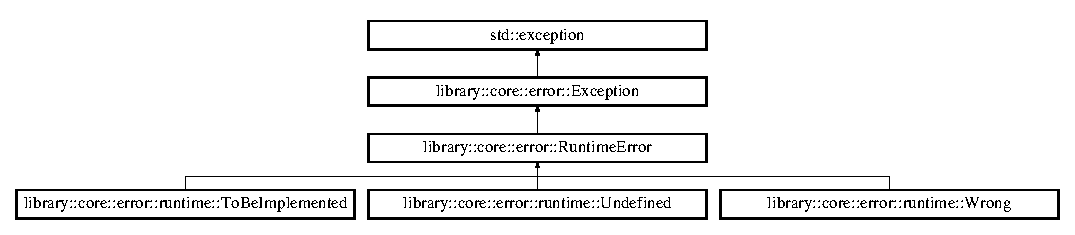
\includegraphics[height=2.715152cm]{classlibrary_1_1core_1_1error_1_1_runtime_error}
\end{center}
\end{figure}
\subsection*{Public Member Functions}
\begin{DoxyCompactItemize}
\item 
\hyperlink{classlibrary_1_1core_1_1error_1_1_runtime_error_a6ba0ac577d200ad5f83843ecbe775c2f}{Runtime\+Error} (const \hyperlink{classlibrary_1_1core_1_1types_1_1_string}{String} \&a\+Message)
\item 
{\footnotesize template$<$typename ... Args$>$ }\\\hyperlink{classlibrary_1_1core_1_1error_1_1_runtime_error_a4ac1bac63f4c46fe10e7c96d545c6e4a}{Runtime\+Error} (const char $\ast$a\+Format, Args... an\+Argument\+List)
\item 
\hyperlink{classlibrary_1_1core_1_1error_1_1_runtime_error_ab66a0df8767bf53b9910a15960622c0d}{$\sim$\+Runtime\+Error} ()
\item 
virtual const char $\ast$ \hyperlink{classlibrary_1_1core_1_1error_1_1_runtime_error_af3da31cf67f3f5e120c5db9072e3a801}{what} () const noexcept override
\end{DoxyCompactItemize}


\subsection{Detailed Description}
Runtime error class. 

\subsection{Constructor \& Destructor Documentation}
\mbox{\Hypertarget{classlibrary_1_1core_1_1error_1_1_runtime_error_a6ba0ac577d200ad5f83843ecbe775c2f}\label{classlibrary_1_1core_1_1error_1_1_runtime_error_a6ba0ac577d200ad5f83843ecbe775c2f}} 
\index{library\+::core\+::error\+::\+Runtime\+Error@{library\+::core\+::error\+::\+Runtime\+Error}!Runtime\+Error@{Runtime\+Error}}
\index{Runtime\+Error@{Runtime\+Error}!library\+::core\+::error\+::\+Runtime\+Error@{library\+::core\+::error\+::\+Runtime\+Error}}
\subsubsection{\texorpdfstring{Runtime\+Error()}{RuntimeError()}\hspace{0.1cm}{\footnotesize\ttfamily [1/2]}}
{\footnotesize\ttfamily library\+::core\+::error\+::\+Runtime\+Error\+::\+Runtime\+Error (\begin{DoxyParamCaption}\item[{const \hyperlink{classlibrary_1_1core_1_1types_1_1_string}{String} \&}]{a\+Message }\end{DoxyParamCaption})}

\mbox{\Hypertarget{classlibrary_1_1core_1_1error_1_1_runtime_error_a4ac1bac63f4c46fe10e7c96d545c6e4a}\label{classlibrary_1_1core_1_1error_1_1_runtime_error_a4ac1bac63f4c46fe10e7c96d545c6e4a}} 
\index{library\+::core\+::error\+::\+Runtime\+Error@{library\+::core\+::error\+::\+Runtime\+Error}!Runtime\+Error@{Runtime\+Error}}
\index{Runtime\+Error@{Runtime\+Error}!library\+::core\+::error\+::\+Runtime\+Error@{library\+::core\+::error\+::\+Runtime\+Error}}
\subsubsection{\texorpdfstring{Runtime\+Error()}{RuntimeError()}\hspace{0.1cm}{\footnotesize\ttfamily [2/2]}}
{\footnotesize\ttfamily template$<$typename ... Args$>$ \\
library\+::core\+::error\+::\+Runtime\+Error\+::\+Runtime\+Error (\begin{DoxyParamCaption}\item[{const char $\ast$}]{a\+Format,  }\item[{Args...}]{an\+Argument\+List }\end{DoxyParamCaption})\hspace{0.3cm}{\ttfamily [inline]}}

\mbox{\Hypertarget{classlibrary_1_1core_1_1error_1_1_runtime_error_ab66a0df8767bf53b9910a15960622c0d}\label{classlibrary_1_1core_1_1error_1_1_runtime_error_ab66a0df8767bf53b9910a15960622c0d}} 
\index{library\+::core\+::error\+::\+Runtime\+Error@{library\+::core\+::error\+::\+Runtime\+Error}!````~Runtime\+Error@{$\sim$\+Runtime\+Error}}
\index{````~Runtime\+Error@{$\sim$\+Runtime\+Error}!library\+::core\+::error\+::\+Runtime\+Error@{library\+::core\+::error\+::\+Runtime\+Error}}
\subsubsection{\texorpdfstring{$\sim$\+Runtime\+Error()}{~RuntimeError()}}
{\footnotesize\ttfamily library\+::core\+::error\+::\+Runtime\+Error\+::$\sim$\+Runtime\+Error (\begin{DoxyParamCaption}{ }\end{DoxyParamCaption})}



\subsection{Member Function Documentation}
\mbox{\Hypertarget{classlibrary_1_1core_1_1error_1_1_runtime_error_af3da31cf67f3f5e120c5db9072e3a801}\label{classlibrary_1_1core_1_1error_1_1_runtime_error_af3da31cf67f3f5e120c5db9072e3a801}} 
\index{library\+::core\+::error\+::\+Runtime\+Error@{library\+::core\+::error\+::\+Runtime\+Error}!what@{what}}
\index{what@{what}!library\+::core\+::error\+::\+Runtime\+Error@{library\+::core\+::error\+::\+Runtime\+Error}}
\subsubsection{\texorpdfstring{what()}{what()}}
{\footnotesize\ttfamily const char $\ast$ library\+::core\+::error\+::\+Runtime\+Error\+::what (\begin{DoxyParamCaption}{ }\end{DoxyParamCaption}) const\hspace{0.3cm}{\ttfamily [override]}, {\ttfamily [virtual]}, {\ttfamily [noexcept]}}



Reimplemented from \hyperlink{classlibrary_1_1core_1_1error_1_1_exception_ab318a927162519b15961ca66be07fd6b}{library\+::core\+::error\+::\+Exception}.



The documentation for this class was generated from the following files\+:\begin{DoxyCompactItemize}
\item 
include/\+Library/\+Core/\+Error/\hyperlink{_runtime_error_8hpp}{Runtime\+Error.\+hpp}\item 
src/\+Library/\+Core/\+Error/\hyperlink{_runtime_error_8cpp}{Runtime\+Error.\+cpp}\end{DoxyCompactItemize}

\hypertarget{classlibrary_1_1core_1_1logger_1_1_sink}{}\section{library\+::core\+::logger\+::Sink Class Reference}
\label{classlibrary_1_1core_1_1logger_1_1_sink}\index{library::core::logger::Sink@{library::core::logger::Sink}}


Log sink.  




{\ttfamily \#include $<$Sink.\+hpp$>$}

\subsection*{Public Member Functions}
\begin{DoxyCompactItemize}
\item 
\mbox{\hyperlink{classlibrary_1_1core_1_1logger_1_1_sink_a9a09bc8eecde876eda9ee3e1a065b638}{Sink}} (const \mbox{\hyperlink{classlibrary_1_1core_1_1logger_1_1sinks_1_1_sink}{sinks\+::\+Sink}} \&a\+Sink)
\item 
\mbox{\hyperlink{classlibrary_1_1core_1_1logger_1_1_sink_a078d839c57afa6e0a5c155a453e95239}{Sink}} (const \mbox{\hyperlink{classlibrary_1_1core_1_1logger_1_1_sink}{Sink}} \&a\+Sink)
\item 
void \mbox{\hyperlink{classlibrary_1_1core_1_1logger_1_1_sink_a726fd3b9e1c3a914fd4913d746656202}{enable}} ()
\item 
void \mbox{\hyperlink{classlibrary_1_1core_1_1logger_1_1_sink_a94d8e1a986d1b105623ee86c91ad491c}{disable}} ()
\item 
void \mbox{\hyperlink{classlibrary_1_1core_1_1logger_1_1_sink_a38376215a70240c65c17b1c89b7f7885}{add\+Channel}} (const \mbox{\hyperlink{classlibrary_1_1core_1_1types_1_1_string}{String}} \&a\+Channel)
\item 
void \mbox{\hyperlink{classlibrary_1_1core_1_1logger_1_1_sink_ad10051906ffb85e6980b547a1fddf272}{remove\+Channel}} (const \mbox{\hyperlink{classlibrary_1_1core_1_1types_1_1_string}{String}} \&a\+Channel)
\end{DoxyCompactItemize}
\subsection*{Static Public Member Functions}
\begin{DoxyCompactItemize}
\item 
static \mbox{\hyperlink{classlibrary_1_1core_1_1logger_1_1_sink}{Sink}} \mbox{\hyperlink{classlibrary_1_1core_1_1logger_1_1_sink_ae3a2c4036340751f16a32e428a9c168a}{Console}} (const \mbox{\hyperlink{namespacelibrary_1_1core_1_1logger_a35f71353edf64f68f7fe3874b01abaa8}{Severity}} \&a\+Severity)
\end{DoxyCompactItemize}


\subsection{Detailed Description}
Log sink. 

\subsection{Constructor \& Destructor Documentation}
\mbox{\Hypertarget{classlibrary_1_1core_1_1logger_1_1_sink_a9a09bc8eecde876eda9ee3e1a065b638}\label{classlibrary_1_1core_1_1logger_1_1_sink_a9a09bc8eecde876eda9ee3e1a065b638}} 
\index{library::core::logger::Sink@{library::core::logger::Sink}!Sink@{Sink}}
\index{Sink@{Sink}!library::core::logger::Sink@{library::core::logger::Sink}}
\subsubsection{\texorpdfstring{Sink()}{Sink()}\hspace{0.1cm}{\footnotesize\ttfamily [1/2]}}
{\footnotesize\ttfamily library\+::core\+::logger\+::\+Sink\+::\+Sink (\begin{DoxyParamCaption}\item[{const \mbox{\hyperlink{classlibrary_1_1core_1_1logger_1_1sinks_1_1_sink}{sinks\+::\+Sink}} \&}]{a\+Sink }\end{DoxyParamCaption})}

\mbox{\Hypertarget{classlibrary_1_1core_1_1logger_1_1_sink_a078d839c57afa6e0a5c155a453e95239}\label{classlibrary_1_1core_1_1logger_1_1_sink_a078d839c57afa6e0a5c155a453e95239}} 
\index{library::core::logger::Sink@{library::core::logger::Sink}!Sink@{Sink}}
\index{Sink@{Sink}!library::core::logger::Sink@{library::core::logger::Sink}}
\subsubsection{\texorpdfstring{Sink()}{Sink()}\hspace{0.1cm}{\footnotesize\ttfamily [2/2]}}
{\footnotesize\ttfamily library\+::core\+::logger\+::\+Sink\+::\+Sink (\begin{DoxyParamCaption}\item[{const \mbox{\hyperlink{classlibrary_1_1core_1_1logger_1_1_sink}{Sink}} \&}]{a\+Sink }\end{DoxyParamCaption})}



\subsection{Member Function Documentation}
\mbox{\Hypertarget{classlibrary_1_1core_1_1logger_1_1_sink_a38376215a70240c65c17b1c89b7f7885}\label{classlibrary_1_1core_1_1logger_1_1_sink_a38376215a70240c65c17b1c89b7f7885}} 
\index{library::core::logger::Sink@{library::core::logger::Sink}!addChannel@{addChannel}}
\index{addChannel@{addChannel}!library::core::logger::Sink@{library::core::logger::Sink}}
\subsubsection{\texorpdfstring{addChannel()}{addChannel()}}
{\footnotesize\ttfamily void library\+::core\+::logger\+::\+Sink\+::add\+Channel (\begin{DoxyParamCaption}\item[{const \mbox{\hyperlink{classlibrary_1_1core_1_1types_1_1_string}{String}} \&}]{a\+Channel }\end{DoxyParamCaption})}

\mbox{\Hypertarget{classlibrary_1_1core_1_1logger_1_1_sink_ae3a2c4036340751f16a32e428a9c168a}\label{classlibrary_1_1core_1_1logger_1_1_sink_ae3a2c4036340751f16a32e428a9c168a}} 
\index{library::core::logger::Sink@{library::core::logger::Sink}!Console@{Console}}
\index{Console@{Console}!library::core::logger::Sink@{library::core::logger::Sink}}
\subsubsection{\texorpdfstring{Console()}{Console()}}
{\footnotesize\ttfamily static \mbox{\hyperlink{classlibrary_1_1core_1_1logger_1_1_sink}{Sink}} library\+::core\+::logger\+::\+Sink\+::\+Console (\begin{DoxyParamCaption}\item[{const \mbox{\hyperlink{namespacelibrary_1_1core_1_1logger_a35f71353edf64f68f7fe3874b01abaa8}{Severity}} \&}]{a\+Severity }\end{DoxyParamCaption})\hspace{0.3cm}{\ttfamily [static]}}

\mbox{\Hypertarget{classlibrary_1_1core_1_1logger_1_1_sink_a94d8e1a986d1b105623ee86c91ad491c}\label{classlibrary_1_1core_1_1logger_1_1_sink_a94d8e1a986d1b105623ee86c91ad491c}} 
\index{library::core::logger::Sink@{library::core::logger::Sink}!disable@{disable}}
\index{disable@{disable}!library::core::logger::Sink@{library::core::logger::Sink}}
\subsubsection{\texorpdfstring{disable()}{disable()}}
{\footnotesize\ttfamily void library\+::core\+::logger\+::\+Sink\+::disable (\begin{DoxyParamCaption}{ }\end{DoxyParamCaption})}

\mbox{\Hypertarget{classlibrary_1_1core_1_1logger_1_1_sink_a726fd3b9e1c3a914fd4913d746656202}\label{classlibrary_1_1core_1_1logger_1_1_sink_a726fd3b9e1c3a914fd4913d746656202}} 
\index{library::core::logger::Sink@{library::core::logger::Sink}!enable@{enable}}
\index{enable@{enable}!library::core::logger::Sink@{library::core::logger::Sink}}
\subsubsection{\texorpdfstring{enable()}{enable()}}
{\footnotesize\ttfamily void library\+::core\+::logger\+::\+Sink\+::enable (\begin{DoxyParamCaption}{ }\end{DoxyParamCaption})}

\mbox{\Hypertarget{classlibrary_1_1core_1_1logger_1_1_sink_ad10051906ffb85e6980b547a1fddf272}\label{classlibrary_1_1core_1_1logger_1_1_sink_ad10051906ffb85e6980b547a1fddf272}} 
\index{library::core::logger::Sink@{library::core::logger::Sink}!removeChannel@{removeChannel}}
\index{removeChannel@{removeChannel}!library::core::logger::Sink@{library::core::logger::Sink}}
\subsubsection{\texorpdfstring{removeChannel()}{removeChannel()}}
{\footnotesize\ttfamily void library\+::core\+::logger\+::\+Sink\+::remove\+Channel (\begin{DoxyParamCaption}\item[{const \mbox{\hyperlink{classlibrary_1_1core_1_1types_1_1_string}{String}} \&}]{a\+Channel }\end{DoxyParamCaption})}



The documentation for this class was generated from the following file\+:\begin{DoxyCompactItemize}
\item 
include/\+Library/\+Core/\+Logger/\mbox{\hyperlink{_sink_8hpp}{Sink.\+hpp}}\end{DoxyCompactItemize}

\hypertarget{classlibrary_1_1core_1_1logger_1_1sinks_1_1_sink}{}\section{library\+:\+:core\+:\+:logger\+:\+:sinks\+:\+:Sink Class Reference}
\label{classlibrary_1_1core_1_1logger_1_1sinks_1_1_sink}\index{library\+::core\+::logger\+::sinks\+::\+Sink@{library\+::core\+::logger\+::sinks\+::\+Sink}}


Log sink base.  




{\ttfamily \#include $<$Sink.\+hpp$>$}

Inheritance diagram for library\+:\+:core\+:\+:logger\+:\+:sinks\+:\+:Sink\+:\begin{figure}[H]
\begin{center}
\leavevmode
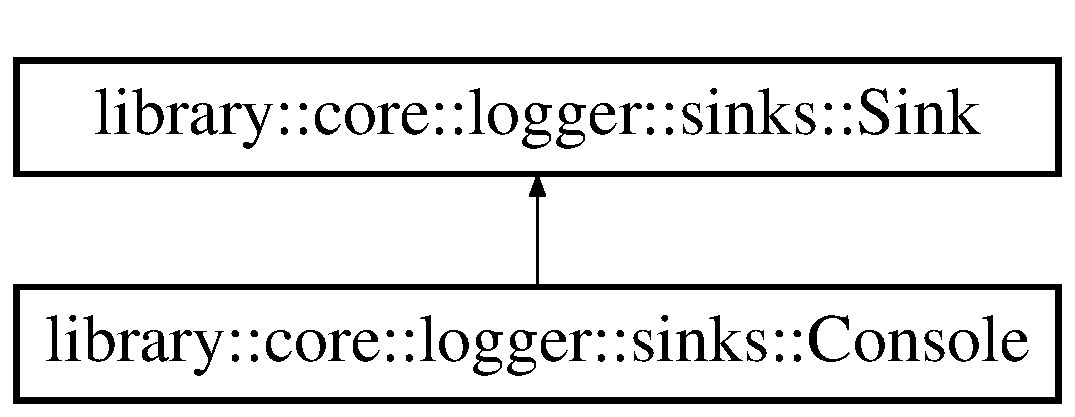
\includegraphics[height=2.000000cm]{classlibrary_1_1core_1_1logger_1_1sinks_1_1_sink}
\end{center}
\end{figure}
\subsection*{Public Member Functions}
\begin{DoxyCompactItemize}
\item 
\hyperlink{classlibrary_1_1core_1_1logger_1_1sinks_1_1_sink_a4d53e570fb2be9c97596289743d0ef9d}{Sink} (const \hyperlink{namespacelibrary_1_1core_1_1logger_a35f71353edf64f68f7fe3874b01abaa8}{Severity} \&a\+Severity)
\item 
virtual \hyperlink{classlibrary_1_1core_1_1logger_1_1sinks_1_1_sink_af00134e95d23ea002acd6dfcc8feed7e}{$\sim$\+Sink} ()=0
\item 
virtual \hyperlink{classlibrary_1_1core_1_1logger_1_1sinks_1_1_sink}{Sink} $\ast$ \hyperlink{classlibrary_1_1core_1_1logger_1_1sinks_1_1_sink_a00ba941947d903825f4922694e0961dd}{clone} () const =0
\item 
bool \hyperlink{classlibrary_1_1core_1_1logger_1_1sinks_1_1_sink_a31a8ad92f76ad05d630d50fe63c1b747}{is\+Enabled} () const
\item 
bool \hyperlink{classlibrary_1_1core_1_1logger_1_1sinks_1_1_sink_a5670a0ee01ffa61fce94ff14b744cda4}{is\+Line\+Id\+Logged} () const
\item 
bool \hyperlink{classlibrary_1_1core_1_1logger_1_1sinks_1_1_sink_af6daeb043af9f1997c04d0e24c12900c}{is\+Severity\+Logged} () const
\item 
bool \hyperlink{classlibrary_1_1core_1_1logger_1_1sinks_1_1_sink_ae9a663485069c6716bb3675d67bd6cd6}{is\+Timestamp\+Logged} () const
\item 
bool \hyperlink{classlibrary_1_1core_1_1logger_1_1sinks_1_1_sink_afdf81adfa6c595d8014b466d86479fae}{is\+Thread\+Logged} () const
\item 
bool \hyperlink{classlibrary_1_1core_1_1logger_1_1sinks_1_1_sink_a09eb7bc8611effd50151c5e371a5962c}{is\+Scope\+Logged} () const
\item 
bool \hyperlink{classlibrary_1_1core_1_1logger_1_1sinks_1_1_sink_a736086840b9c964c40e349d5e7f68cca}{is\+File\+Logged} () const
\item 
bool \hyperlink{classlibrary_1_1core_1_1logger_1_1sinks_1_1_sink_a701bbd71bc5f871ac97abdc98fa4460f}{is\+Line\+Logged} () const
\item 
bool \hyperlink{classlibrary_1_1core_1_1logger_1_1sinks_1_1_sink_a39078847a7c0f6a22893dd82e64545f1}{is\+Function\+Logged} () const
\item 
bool \hyperlink{classlibrary_1_1core_1_1logger_1_1sinks_1_1_sink_a708041f4c444c21ea1963bd0649b6ac5}{is\+Channel\+Logged} () const
\item 
virtual void \hyperlink{classlibrary_1_1core_1_1logger_1_1sinks_1_1_sink_aa41e2b1488d2e761ded1d209eacf02b3}{enable} ()=0
\item 
virtual void \hyperlink{classlibrary_1_1core_1_1logger_1_1sinks_1_1_sink_a3ab28f7a964d138fc9d080f026bb4143}{disable} ()=0
\item 
void \hyperlink{classlibrary_1_1core_1_1logger_1_1sinks_1_1_sink_a7905264ef5dde58d967fd7ebb011bdf9}{add\+Channel} (const \hyperlink{classlibrary_1_1core_1_1types_1_1_string}{String} \&a\+Channel)
\item 
void \hyperlink{classlibrary_1_1core_1_1logger_1_1sinks_1_1_sink_a5dd0f0385cd5ba7d281864ba6b8ff7a7}{remove\+Channel} (const \hyperlink{classlibrary_1_1core_1_1types_1_1_string}{String} \&a\+Channel)
\end{DoxyCompactItemize}
\subsection*{Protected Attributes}
\begin{DoxyCompactItemize}
\item 
bool \hyperlink{classlibrary_1_1core_1_1logger_1_1sinks_1_1_sink_ac1386fd47307e8956c345b5ec5725c8f}{enabled\+\_\+}
\item 
\hyperlink{namespacelibrary_1_1core_1_1logger_a35f71353edf64f68f7fe3874b01abaa8}{Severity} \hyperlink{classlibrary_1_1core_1_1logger_1_1sinks_1_1_sink_a49cd9c83a41cde12c4b0f5431c0e1b41}{severity\+\_\+}
\item 
bool \hyperlink{classlibrary_1_1core_1_1logger_1_1sinks_1_1_sink_a75d2b3e0a9551cd8788e3d9c320d79dd}{line\+Id\+Enabled\+\_\+}
\item 
bool \hyperlink{classlibrary_1_1core_1_1logger_1_1sinks_1_1_sink_af54f11a79fe19b15f2bc2f3783d382ba}{severity\+Enabled\+\_\+}
\item 
bool \hyperlink{classlibrary_1_1core_1_1logger_1_1sinks_1_1_sink_afebb8b5eef5abf365943cd10caf23bab}{timestamp\+Enabled\+\_\+}
\item 
bool \hyperlink{classlibrary_1_1core_1_1logger_1_1sinks_1_1_sink_abf1a3577855cc40b5075b4d73a3c86a2}{thread\+Enabled\+\_\+}
\item 
bool \hyperlink{classlibrary_1_1core_1_1logger_1_1sinks_1_1_sink_abffe5eb81e1eb858eaad2cc806b3806b}{scope\+Enabled\+\_\+}
\item 
bool \hyperlink{classlibrary_1_1core_1_1logger_1_1sinks_1_1_sink_a8691bad7f4c73aa394901e6e10b5fe47}{file\+Enabled\+\_\+}
\item 
bool \hyperlink{classlibrary_1_1core_1_1logger_1_1sinks_1_1_sink_a00b45879a45459f44475eab2618b30f9}{line\+Enabled\+\_\+}
\item 
bool \hyperlink{classlibrary_1_1core_1_1logger_1_1sinks_1_1_sink_acb68b94fd8745d1e06d1cc1f2caa2e73}{function\+Enabled\+\_\+}
\item 
bool \hyperlink{classlibrary_1_1core_1_1logger_1_1sinks_1_1_sink_a48307be32eede5359f345b54363070ae}{channel\+Enabled\+\_\+}
\item 
\hyperlink{classlibrary_1_1core_1_1ctnr_1_1_array}{Array}$<$ \hyperlink{classlibrary_1_1core_1_1types_1_1_string}{String} $>$ \hyperlink{classlibrary_1_1core_1_1logger_1_1sinks_1_1_sink_a3ba1eb6372e9bf6d2d8b3ff53d529021}{channels\+\_\+}
\end{DoxyCompactItemize}


\subsection{Detailed Description}
Log sink base. 

\subsection{Constructor \& Destructor Documentation}
\mbox{\Hypertarget{classlibrary_1_1core_1_1logger_1_1sinks_1_1_sink_a4d53e570fb2be9c97596289743d0ef9d}\label{classlibrary_1_1core_1_1logger_1_1sinks_1_1_sink_a4d53e570fb2be9c97596289743d0ef9d}} 
\index{library\+::core\+::logger\+::sinks\+::\+Sink@{library\+::core\+::logger\+::sinks\+::\+Sink}!Sink@{Sink}}
\index{Sink@{Sink}!library\+::core\+::logger\+::sinks\+::\+Sink@{library\+::core\+::logger\+::sinks\+::\+Sink}}
\subsubsection{\texorpdfstring{Sink()}{Sink()}}
{\footnotesize\ttfamily library\+::core\+::logger\+::sinks\+::\+Sink\+::\+Sink (\begin{DoxyParamCaption}\item[{const \hyperlink{namespacelibrary_1_1core_1_1logger_a35f71353edf64f68f7fe3874b01abaa8}{Severity} \&}]{a\+Severity }\end{DoxyParamCaption})}

\mbox{\Hypertarget{classlibrary_1_1core_1_1logger_1_1sinks_1_1_sink_af00134e95d23ea002acd6dfcc8feed7e}\label{classlibrary_1_1core_1_1logger_1_1sinks_1_1_sink_af00134e95d23ea002acd6dfcc8feed7e}} 
\index{library\+::core\+::logger\+::sinks\+::\+Sink@{library\+::core\+::logger\+::sinks\+::\+Sink}!````~Sink@{$\sim$\+Sink}}
\index{````~Sink@{$\sim$\+Sink}!library\+::core\+::logger\+::sinks\+::\+Sink@{library\+::core\+::logger\+::sinks\+::\+Sink}}
\subsubsection{\texorpdfstring{$\sim$\+Sink()}{~Sink()}}
{\footnotesize\ttfamily virtual library\+::core\+::logger\+::sinks\+::\+Sink\+::$\sim$\+Sink (\begin{DoxyParamCaption}{ }\end{DoxyParamCaption})\hspace{0.3cm}{\ttfamily [pure virtual]}}



\subsection{Member Function Documentation}
\mbox{\Hypertarget{classlibrary_1_1core_1_1logger_1_1sinks_1_1_sink_a7905264ef5dde58d967fd7ebb011bdf9}\label{classlibrary_1_1core_1_1logger_1_1sinks_1_1_sink_a7905264ef5dde58d967fd7ebb011bdf9}} 
\index{library\+::core\+::logger\+::sinks\+::\+Sink@{library\+::core\+::logger\+::sinks\+::\+Sink}!add\+Channel@{add\+Channel}}
\index{add\+Channel@{add\+Channel}!library\+::core\+::logger\+::sinks\+::\+Sink@{library\+::core\+::logger\+::sinks\+::\+Sink}}
\subsubsection{\texorpdfstring{add\+Channel()}{addChannel()}}
{\footnotesize\ttfamily void library\+::core\+::logger\+::sinks\+::\+Sink\+::add\+Channel (\begin{DoxyParamCaption}\item[{const \hyperlink{classlibrary_1_1core_1_1types_1_1_string}{String} \&}]{a\+Channel }\end{DoxyParamCaption})}

\mbox{\Hypertarget{classlibrary_1_1core_1_1logger_1_1sinks_1_1_sink_a00ba941947d903825f4922694e0961dd}\label{classlibrary_1_1core_1_1logger_1_1sinks_1_1_sink_a00ba941947d903825f4922694e0961dd}} 
\index{library\+::core\+::logger\+::sinks\+::\+Sink@{library\+::core\+::logger\+::sinks\+::\+Sink}!clone@{clone}}
\index{clone@{clone}!library\+::core\+::logger\+::sinks\+::\+Sink@{library\+::core\+::logger\+::sinks\+::\+Sink}}
\subsubsection{\texorpdfstring{clone()}{clone()}}
{\footnotesize\ttfamily virtual \hyperlink{classlibrary_1_1core_1_1logger_1_1sinks_1_1_sink}{Sink}$\ast$ library\+::core\+::logger\+::sinks\+::\+Sink\+::clone (\begin{DoxyParamCaption}{ }\end{DoxyParamCaption}) const\hspace{0.3cm}{\ttfamily [pure virtual]}}



Implemented in \hyperlink{classlibrary_1_1core_1_1logger_1_1sinks_1_1_console_ac5c80193b0832f760a7447e7abc7d468}{library\+::core\+::logger\+::sinks\+::\+Console}.

\mbox{\Hypertarget{classlibrary_1_1core_1_1logger_1_1sinks_1_1_sink_a3ab28f7a964d138fc9d080f026bb4143}\label{classlibrary_1_1core_1_1logger_1_1sinks_1_1_sink_a3ab28f7a964d138fc9d080f026bb4143}} 
\index{library\+::core\+::logger\+::sinks\+::\+Sink@{library\+::core\+::logger\+::sinks\+::\+Sink}!disable@{disable}}
\index{disable@{disable}!library\+::core\+::logger\+::sinks\+::\+Sink@{library\+::core\+::logger\+::sinks\+::\+Sink}}
\subsubsection{\texorpdfstring{disable()}{disable()}}
{\footnotesize\ttfamily virtual void library\+::core\+::logger\+::sinks\+::\+Sink\+::disable (\begin{DoxyParamCaption}{ }\end{DoxyParamCaption})\hspace{0.3cm}{\ttfamily [pure virtual]}}



Implemented in \hyperlink{classlibrary_1_1core_1_1logger_1_1sinks_1_1_console_adc1a648433f26cc4397f1e703c9506c7}{library\+::core\+::logger\+::sinks\+::\+Console}.

\mbox{\Hypertarget{classlibrary_1_1core_1_1logger_1_1sinks_1_1_sink_aa41e2b1488d2e761ded1d209eacf02b3}\label{classlibrary_1_1core_1_1logger_1_1sinks_1_1_sink_aa41e2b1488d2e761ded1d209eacf02b3}} 
\index{library\+::core\+::logger\+::sinks\+::\+Sink@{library\+::core\+::logger\+::sinks\+::\+Sink}!enable@{enable}}
\index{enable@{enable}!library\+::core\+::logger\+::sinks\+::\+Sink@{library\+::core\+::logger\+::sinks\+::\+Sink}}
\subsubsection{\texorpdfstring{enable()}{enable()}}
{\footnotesize\ttfamily virtual void library\+::core\+::logger\+::sinks\+::\+Sink\+::enable (\begin{DoxyParamCaption}{ }\end{DoxyParamCaption})\hspace{0.3cm}{\ttfamily [pure virtual]}}



Implemented in \hyperlink{classlibrary_1_1core_1_1logger_1_1sinks_1_1_console_a09190fa0b66fa9a03792e6a546590da9}{library\+::core\+::logger\+::sinks\+::\+Console}.

\mbox{\Hypertarget{classlibrary_1_1core_1_1logger_1_1sinks_1_1_sink_a708041f4c444c21ea1963bd0649b6ac5}\label{classlibrary_1_1core_1_1logger_1_1sinks_1_1_sink_a708041f4c444c21ea1963bd0649b6ac5}} 
\index{library\+::core\+::logger\+::sinks\+::\+Sink@{library\+::core\+::logger\+::sinks\+::\+Sink}!is\+Channel\+Logged@{is\+Channel\+Logged}}
\index{is\+Channel\+Logged@{is\+Channel\+Logged}!library\+::core\+::logger\+::sinks\+::\+Sink@{library\+::core\+::logger\+::sinks\+::\+Sink}}
\subsubsection{\texorpdfstring{is\+Channel\+Logged()}{isChannelLogged()}}
{\footnotesize\ttfamily bool library\+::core\+::logger\+::sinks\+::\+Sink\+::is\+Channel\+Logged (\begin{DoxyParamCaption}{ }\end{DoxyParamCaption}) const}

\mbox{\Hypertarget{classlibrary_1_1core_1_1logger_1_1sinks_1_1_sink_a31a8ad92f76ad05d630d50fe63c1b747}\label{classlibrary_1_1core_1_1logger_1_1sinks_1_1_sink_a31a8ad92f76ad05d630d50fe63c1b747}} 
\index{library\+::core\+::logger\+::sinks\+::\+Sink@{library\+::core\+::logger\+::sinks\+::\+Sink}!is\+Enabled@{is\+Enabled}}
\index{is\+Enabled@{is\+Enabled}!library\+::core\+::logger\+::sinks\+::\+Sink@{library\+::core\+::logger\+::sinks\+::\+Sink}}
\subsubsection{\texorpdfstring{is\+Enabled()}{isEnabled()}}
{\footnotesize\ttfamily bool library\+::core\+::logger\+::sinks\+::\+Sink\+::is\+Enabled (\begin{DoxyParamCaption}{ }\end{DoxyParamCaption}) const}

\mbox{\Hypertarget{classlibrary_1_1core_1_1logger_1_1sinks_1_1_sink_a736086840b9c964c40e349d5e7f68cca}\label{classlibrary_1_1core_1_1logger_1_1sinks_1_1_sink_a736086840b9c964c40e349d5e7f68cca}} 
\index{library\+::core\+::logger\+::sinks\+::\+Sink@{library\+::core\+::logger\+::sinks\+::\+Sink}!is\+File\+Logged@{is\+File\+Logged}}
\index{is\+File\+Logged@{is\+File\+Logged}!library\+::core\+::logger\+::sinks\+::\+Sink@{library\+::core\+::logger\+::sinks\+::\+Sink}}
\subsubsection{\texorpdfstring{is\+File\+Logged()}{isFileLogged()}}
{\footnotesize\ttfamily bool library\+::core\+::logger\+::sinks\+::\+Sink\+::is\+File\+Logged (\begin{DoxyParamCaption}{ }\end{DoxyParamCaption}) const}

\mbox{\Hypertarget{classlibrary_1_1core_1_1logger_1_1sinks_1_1_sink_a39078847a7c0f6a22893dd82e64545f1}\label{classlibrary_1_1core_1_1logger_1_1sinks_1_1_sink_a39078847a7c0f6a22893dd82e64545f1}} 
\index{library\+::core\+::logger\+::sinks\+::\+Sink@{library\+::core\+::logger\+::sinks\+::\+Sink}!is\+Function\+Logged@{is\+Function\+Logged}}
\index{is\+Function\+Logged@{is\+Function\+Logged}!library\+::core\+::logger\+::sinks\+::\+Sink@{library\+::core\+::logger\+::sinks\+::\+Sink}}
\subsubsection{\texorpdfstring{is\+Function\+Logged()}{isFunctionLogged()}}
{\footnotesize\ttfamily bool library\+::core\+::logger\+::sinks\+::\+Sink\+::is\+Function\+Logged (\begin{DoxyParamCaption}{ }\end{DoxyParamCaption}) const}

\mbox{\Hypertarget{classlibrary_1_1core_1_1logger_1_1sinks_1_1_sink_a5670a0ee01ffa61fce94ff14b744cda4}\label{classlibrary_1_1core_1_1logger_1_1sinks_1_1_sink_a5670a0ee01ffa61fce94ff14b744cda4}} 
\index{library\+::core\+::logger\+::sinks\+::\+Sink@{library\+::core\+::logger\+::sinks\+::\+Sink}!is\+Line\+Id\+Logged@{is\+Line\+Id\+Logged}}
\index{is\+Line\+Id\+Logged@{is\+Line\+Id\+Logged}!library\+::core\+::logger\+::sinks\+::\+Sink@{library\+::core\+::logger\+::sinks\+::\+Sink}}
\subsubsection{\texorpdfstring{is\+Line\+Id\+Logged()}{isLineIdLogged()}}
{\footnotesize\ttfamily bool library\+::core\+::logger\+::sinks\+::\+Sink\+::is\+Line\+Id\+Logged (\begin{DoxyParamCaption}{ }\end{DoxyParamCaption}) const}

\mbox{\Hypertarget{classlibrary_1_1core_1_1logger_1_1sinks_1_1_sink_a701bbd71bc5f871ac97abdc98fa4460f}\label{classlibrary_1_1core_1_1logger_1_1sinks_1_1_sink_a701bbd71bc5f871ac97abdc98fa4460f}} 
\index{library\+::core\+::logger\+::sinks\+::\+Sink@{library\+::core\+::logger\+::sinks\+::\+Sink}!is\+Line\+Logged@{is\+Line\+Logged}}
\index{is\+Line\+Logged@{is\+Line\+Logged}!library\+::core\+::logger\+::sinks\+::\+Sink@{library\+::core\+::logger\+::sinks\+::\+Sink}}
\subsubsection{\texorpdfstring{is\+Line\+Logged()}{isLineLogged()}}
{\footnotesize\ttfamily bool library\+::core\+::logger\+::sinks\+::\+Sink\+::is\+Line\+Logged (\begin{DoxyParamCaption}{ }\end{DoxyParamCaption}) const}

\mbox{\Hypertarget{classlibrary_1_1core_1_1logger_1_1sinks_1_1_sink_a09eb7bc8611effd50151c5e371a5962c}\label{classlibrary_1_1core_1_1logger_1_1sinks_1_1_sink_a09eb7bc8611effd50151c5e371a5962c}} 
\index{library\+::core\+::logger\+::sinks\+::\+Sink@{library\+::core\+::logger\+::sinks\+::\+Sink}!is\+Scope\+Logged@{is\+Scope\+Logged}}
\index{is\+Scope\+Logged@{is\+Scope\+Logged}!library\+::core\+::logger\+::sinks\+::\+Sink@{library\+::core\+::logger\+::sinks\+::\+Sink}}
\subsubsection{\texorpdfstring{is\+Scope\+Logged()}{isScopeLogged()}}
{\footnotesize\ttfamily bool library\+::core\+::logger\+::sinks\+::\+Sink\+::is\+Scope\+Logged (\begin{DoxyParamCaption}{ }\end{DoxyParamCaption}) const}

\mbox{\Hypertarget{classlibrary_1_1core_1_1logger_1_1sinks_1_1_sink_af6daeb043af9f1997c04d0e24c12900c}\label{classlibrary_1_1core_1_1logger_1_1sinks_1_1_sink_af6daeb043af9f1997c04d0e24c12900c}} 
\index{library\+::core\+::logger\+::sinks\+::\+Sink@{library\+::core\+::logger\+::sinks\+::\+Sink}!is\+Severity\+Logged@{is\+Severity\+Logged}}
\index{is\+Severity\+Logged@{is\+Severity\+Logged}!library\+::core\+::logger\+::sinks\+::\+Sink@{library\+::core\+::logger\+::sinks\+::\+Sink}}
\subsubsection{\texorpdfstring{is\+Severity\+Logged()}{isSeverityLogged()}}
{\footnotesize\ttfamily bool library\+::core\+::logger\+::sinks\+::\+Sink\+::is\+Severity\+Logged (\begin{DoxyParamCaption}{ }\end{DoxyParamCaption}) const}

\mbox{\Hypertarget{classlibrary_1_1core_1_1logger_1_1sinks_1_1_sink_afdf81adfa6c595d8014b466d86479fae}\label{classlibrary_1_1core_1_1logger_1_1sinks_1_1_sink_afdf81adfa6c595d8014b466d86479fae}} 
\index{library\+::core\+::logger\+::sinks\+::\+Sink@{library\+::core\+::logger\+::sinks\+::\+Sink}!is\+Thread\+Logged@{is\+Thread\+Logged}}
\index{is\+Thread\+Logged@{is\+Thread\+Logged}!library\+::core\+::logger\+::sinks\+::\+Sink@{library\+::core\+::logger\+::sinks\+::\+Sink}}
\subsubsection{\texorpdfstring{is\+Thread\+Logged()}{isThreadLogged()}}
{\footnotesize\ttfamily bool library\+::core\+::logger\+::sinks\+::\+Sink\+::is\+Thread\+Logged (\begin{DoxyParamCaption}{ }\end{DoxyParamCaption}) const}

\mbox{\Hypertarget{classlibrary_1_1core_1_1logger_1_1sinks_1_1_sink_ae9a663485069c6716bb3675d67bd6cd6}\label{classlibrary_1_1core_1_1logger_1_1sinks_1_1_sink_ae9a663485069c6716bb3675d67bd6cd6}} 
\index{library\+::core\+::logger\+::sinks\+::\+Sink@{library\+::core\+::logger\+::sinks\+::\+Sink}!is\+Timestamp\+Logged@{is\+Timestamp\+Logged}}
\index{is\+Timestamp\+Logged@{is\+Timestamp\+Logged}!library\+::core\+::logger\+::sinks\+::\+Sink@{library\+::core\+::logger\+::sinks\+::\+Sink}}
\subsubsection{\texorpdfstring{is\+Timestamp\+Logged()}{isTimestampLogged()}}
{\footnotesize\ttfamily bool library\+::core\+::logger\+::sinks\+::\+Sink\+::is\+Timestamp\+Logged (\begin{DoxyParamCaption}{ }\end{DoxyParamCaption}) const}

\mbox{\Hypertarget{classlibrary_1_1core_1_1logger_1_1sinks_1_1_sink_a5dd0f0385cd5ba7d281864ba6b8ff7a7}\label{classlibrary_1_1core_1_1logger_1_1sinks_1_1_sink_a5dd0f0385cd5ba7d281864ba6b8ff7a7}} 
\index{library\+::core\+::logger\+::sinks\+::\+Sink@{library\+::core\+::logger\+::sinks\+::\+Sink}!remove\+Channel@{remove\+Channel}}
\index{remove\+Channel@{remove\+Channel}!library\+::core\+::logger\+::sinks\+::\+Sink@{library\+::core\+::logger\+::sinks\+::\+Sink}}
\subsubsection{\texorpdfstring{remove\+Channel()}{removeChannel()}}
{\footnotesize\ttfamily void library\+::core\+::logger\+::sinks\+::\+Sink\+::remove\+Channel (\begin{DoxyParamCaption}\item[{const \hyperlink{classlibrary_1_1core_1_1types_1_1_string}{String} \&}]{a\+Channel }\end{DoxyParamCaption})}



\subsection{Member Data Documentation}
\mbox{\Hypertarget{classlibrary_1_1core_1_1logger_1_1sinks_1_1_sink_a48307be32eede5359f345b54363070ae}\label{classlibrary_1_1core_1_1logger_1_1sinks_1_1_sink_a48307be32eede5359f345b54363070ae}} 
\index{library\+::core\+::logger\+::sinks\+::\+Sink@{library\+::core\+::logger\+::sinks\+::\+Sink}!channel\+Enabled\+\_\+@{channel\+Enabled\+\_\+}}
\index{channel\+Enabled\+\_\+@{channel\+Enabled\+\_\+}!library\+::core\+::logger\+::sinks\+::\+Sink@{library\+::core\+::logger\+::sinks\+::\+Sink}}
\subsubsection{\texorpdfstring{channel\+Enabled\+\_\+}{channelEnabled\_}}
{\footnotesize\ttfamily bool library\+::core\+::logger\+::sinks\+::\+Sink\+::channel\+Enabled\+\_\+\hspace{0.3cm}{\ttfamily [protected]}}

\mbox{\Hypertarget{classlibrary_1_1core_1_1logger_1_1sinks_1_1_sink_a3ba1eb6372e9bf6d2d8b3ff53d529021}\label{classlibrary_1_1core_1_1logger_1_1sinks_1_1_sink_a3ba1eb6372e9bf6d2d8b3ff53d529021}} 
\index{library\+::core\+::logger\+::sinks\+::\+Sink@{library\+::core\+::logger\+::sinks\+::\+Sink}!channels\+\_\+@{channels\+\_\+}}
\index{channels\+\_\+@{channels\+\_\+}!library\+::core\+::logger\+::sinks\+::\+Sink@{library\+::core\+::logger\+::sinks\+::\+Sink}}
\subsubsection{\texorpdfstring{channels\+\_\+}{channels\_}}
{\footnotesize\ttfamily \hyperlink{classlibrary_1_1core_1_1ctnr_1_1_array}{Array}$<$\hyperlink{classlibrary_1_1core_1_1types_1_1_string}{String}$>$ library\+::core\+::logger\+::sinks\+::\+Sink\+::channels\+\_\+\hspace{0.3cm}{\ttfamily [protected]}}

\mbox{\Hypertarget{classlibrary_1_1core_1_1logger_1_1sinks_1_1_sink_ac1386fd47307e8956c345b5ec5725c8f}\label{classlibrary_1_1core_1_1logger_1_1sinks_1_1_sink_ac1386fd47307e8956c345b5ec5725c8f}} 
\index{library\+::core\+::logger\+::sinks\+::\+Sink@{library\+::core\+::logger\+::sinks\+::\+Sink}!enabled\+\_\+@{enabled\+\_\+}}
\index{enabled\+\_\+@{enabled\+\_\+}!library\+::core\+::logger\+::sinks\+::\+Sink@{library\+::core\+::logger\+::sinks\+::\+Sink}}
\subsubsection{\texorpdfstring{enabled\+\_\+}{enabled\_}}
{\footnotesize\ttfamily bool library\+::core\+::logger\+::sinks\+::\+Sink\+::enabled\+\_\+\hspace{0.3cm}{\ttfamily [protected]}}

\mbox{\Hypertarget{classlibrary_1_1core_1_1logger_1_1sinks_1_1_sink_a8691bad7f4c73aa394901e6e10b5fe47}\label{classlibrary_1_1core_1_1logger_1_1sinks_1_1_sink_a8691bad7f4c73aa394901e6e10b5fe47}} 
\index{library\+::core\+::logger\+::sinks\+::\+Sink@{library\+::core\+::logger\+::sinks\+::\+Sink}!file\+Enabled\+\_\+@{file\+Enabled\+\_\+}}
\index{file\+Enabled\+\_\+@{file\+Enabled\+\_\+}!library\+::core\+::logger\+::sinks\+::\+Sink@{library\+::core\+::logger\+::sinks\+::\+Sink}}
\subsubsection{\texorpdfstring{file\+Enabled\+\_\+}{fileEnabled\_}}
{\footnotesize\ttfamily bool library\+::core\+::logger\+::sinks\+::\+Sink\+::file\+Enabled\+\_\+\hspace{0.3cm}{\ttfamily [protected]}}

\mbox{\Hypertarget{classlibrary_1_1core_1_1logger_1_1sinks_1_1_sink_acb68b94fd8745d1e06d1cc1f2caa2e73}\label{classlibrary_1_1core_1_1logger_1_1sinks_1_1_sink_acb68b94fd8745d1e06d1cc1f2caa2e73}} 
\index{library\+::core\+::logger\+::sinks\+::\+Sink@{library\+::core\+::logger\+::sinks\+::\+Sink}!function\+Enabled\+\_\+@{function\+Enabled\+\_\+}}
\index{function\+Enabled\+\_\+@{function\+Enabled\+\_\+}!library\+::core\+::logger\+::sinks\+::\+Sink@{library\+::core\+::logger\+::sinks\+::\+Sink}}
\subsubsection{\texorpdfstring{function\+Enabled\+\_\+}{functionEnabled\_}}
{\footnotesize\ttfamily bool library\+::core\+::logger\+::sinks\+::\+Sink\+::function\+Enabled\+\_\+\hspace{0.3cm}{\ttfamily [protected]}}

\mbox{\Hypertarget{classlibrary_1_1core_1_1logger_1_1sinks_1_1_sink_a00b45879a45459f44475eab2618b30f9}\label{classlibrary_1_1core_1_1logger_1_1sinks_1_1_sink_a00b45879a45459f44475eab2618b30f9}} 
\index{library\+::core\+::logger\+::sinks\+::\+Sink@{library\+::core\+::logger\+::sinks\+::\+Sink}!line\+Enabled\+\_\+@{line\+Enabled\+\_\+}}
\index{line\+Enabled\+\_\+@{line\+Enabled\+\_\+}!library\+::core\+::logger\+::sinks\+::\+Sink@{library\+::core\+::logger\+::sinks\+::\+Sink}}
\subsubsection{\texorpdfstring{line\+Enabled\+\_\+}{lineEnabled\_}}
{\footnotesize\ttfamily bool library\+::core\+::logger\+::sinks\+::\+Sink\+::line\+Enabled\+\_\+\hspace{0.3cm}{\ttfamily [protected]}}

\mbox{\Hypertarget{classlibrary_1_1core_1_1logger_1_1sinks_1_1_sink_a75d2b3e0a9551cd8788e3d9c320d79dd}\label{classlibrary_1_1core_1_1logger_1_1sinks_1_1_sink_a75d2b3e0a9551cd8788e3d9c320d79dd}} 
\index{library\+::core\+::logger\+::sinks\+::\+Sink@{library\+::core\+::logger\+::sinks\+::\+Sink}!line\+Id\+Enabled\+\_\+@{line\+Id\+Enabled\+\_\+}}
\index{line\+Id\+Enabled\+\_\+@{line\+Id\+Enabled\+\_\+}!library\+::core\+::logger\+::sinks\+::\+Sink@{library\+::core\+::logger\+::sinks\+::\+Sink}}
\subsubsection{\texorpdfstring{line\+Id\+Enabled\+\_\+}{lineIdEnabled\_}}
{\footnotesize\ttfamily bool library\+::core\+::logger\+::sinks\+::\+Sink\+::line\+Id\+Enabled\+\_\+\hspace{0.3cm}{\ttfamily [protected]}}

\mbox{\Hypertarget{classlibrary_1_1core_1_1logger_1_1sinks_1_1_sink_abffe5eb81e1eb858eaad2cc806b3806b}\label{classlibrary_1_1core_1_1logger_1_1sinks_1_1_sink_abffe5eb81e1eb858eaad2cc806b3806b}} 
\index{library\+::core\+::logger\+::sinks\+::\+Sink@{library\+::core\+::logger\+::sinks\+::\+Sink}!scope\+Enabled\+\_\+@{scope\+Enabled\+\_\+}}
\index{scope\+Enabled\+\_\+@{scope\+Enabled\+\_\+}!library\+::core\+::logger\+::sinks\+::\+Sink@{library\+::core\+::logger\+::sinks\+::\+Sink}}
\subsubsection{\texorpdfstring{scope\+Enabled\+\_\+}{scopeEnabled\_}}
{\footnotesize\ttfamily bool library\+::core\+::logger\+::sinks\+::\+Sink\+::scope\+Enabled\+\_\+\hspace{0.3cm}{\ttfamily [protected]}}

\mbox{\Hypertarget{classlibrary_1_1core_1_1logger_1_1sinks_1_1_sink_a49cd9c83a41cde12c4b0f5431c0e1b41}\label{classlibrary_1_1core_1_1logger_1_1sinks_1_1_sink_a49cd9c83a41cde12c4b0f5431c0e1b41}} 
\index{library\+::core\+::logger\+::sinks\+::\+Sink@{library\+::core\+::logger\+::sinks\+::\+Sink}!severity\+\_\+@{severity\+\_\+}}
\index{severity\+\_\+@{severity\+\_\+}!library\+::core\+::logger\+::sinks\+::\+Sink@{library\+::core\+::logger\+::sinks\+::\+Sink}}
\subsubsection{\texorpdfstring{severity\+\_\+}{severity\_}}
{\footnotesize\ttfamily \hyperlink{namespacelibrary_1_1core_1_1logger_a35f71353edf64f68f7fe3874b01abaa8}{Severity} library\+::core\+::logger\+::sinks\+::\+Sink\+::severity\+\_\+\hspace{0.3cm}{\ttfamily [protected]}}

\mbox{\Hypertarget{classlibrary_1_1core_1_1logger_1_1sinks_1_1_sink_af54f11a79fe19b15f2bc2f3783d382ba}\label{classlibrary_1_1core_1_1logger_1_1sinks_1_1_sink_af54f11a79fe19b15f2bc2f3783d382ba}} 
\index{library\+::core\+::logger\+::sinks\+::\+Sink@{library\+::core\+::logger\+::sinks\+::\+Sink}!severity\+Enabled\+\_\+@{severity\+Enabled\+\_\+}}
\index{severity\+Enabled\+\_\+@{severity\+Enabled\+\_\+}!library\+::core\+::logger\+::sinks\+::\+Sink@{library\+::core\+::logger\+::sinks\+::\+Sink}}
\subsubsection{\texorpdfstring{severity\+Enabled\+\_\+}{severityEnabled\_}}
{\footnotesize\ttfamily bool library\+::core\+::logger\+::sinks\+::\+Sink\+::severity\+Enabled\+\_\+\hspace{0.3cm}{\ttfamily [protected]}}

\mbox{\Hypertarget{classlibrary_1_1core_1_1logger_1_1sinks_1_1_sink_abf1a3577855cc40b5075b4d73a3c86a2}\label{classlibrary_1_1core_1_1logger_1_1sinks_1_1_sink_abf1a3577855cc40b5075b4d73a3c86a2}} 
\index{library\+::core\+::logger\+::sinks\+::\+Sink@{library\+::core\+::logger\+::sinks\+::\+Sink}!thread\+Enabled\+\_\+@{thread\+Enabled\+\_\+}}
\index{thread\+Enabled\+\_\+@{thread\+Enabled\+\_\+}!library\+::core\+::logger\+::sinks\+::\+Sink@{library\+::core\+::logger\+::sinks\+::\+Sink}}
\subsubsection{\texorpdfstring{thread\+Enabled\+\_\+}{threadEnabled\_}}
{\footnotesize\ttfamily bool library\+::core\+::logger\+::sinks\+::\+Sink\+::thread\+Enabled\+\_\+\hspace{0.3cm}{\ttfamily [protected]}}

\mbox{\Hypertarget{classlibrary_1_1core_1_1logger_1_1sinks_1_1_sink_afebb8b5eef5abf365943cd10caf23bab}\label{classlibrary_1_1core_1_1logger_1_1sinks_1_1_sink_afebb8b5eef5abf365943cd10caf23bab}} 
\index{library\+::core\+::logger\+::sinks\+::\+Sink@{library\+::core\+::logger\+::sinks\+::\+Sink}!timestamp\+Enabled\+\_\+@{timestamp\+Enabled\+\_\+}}
\index{timestamp\+Enabled\+\_\+@{timestamp\+Enabled\+\_\+}!library\+::core\+::logger\+::sinks\+::\+Sink@{library\+::core\+::logger\+::sinks\+::\+Sink}}
\subsubsection{\texorpdfstring{timestamp\+Enabled\+\_\+}{timestampEnabled\_}}
{\footnotesize\ttfamily bool library\+::core\+::logger\+::sinks\+::\+Sink\+::timestamp\+Enabled\+\_\+\hspace{0.3cm}{\ttfamily [protected]}}



The documentation for this class was generated from the following file\+:\begin{DoxyCompactItemize}
\item 
include/\+Library/\+Core/\+Logger/\+Sinks/\hyperlink{_sinks_2_sink_8hpp}{Sink.\+hpp}\end{DoxyCompactItemize}

\hypertarget{classlibrary_1_1core_1_1logger_1_1_source}{}\section{library\+::core\+::logger\+::Source Class Reference}
\label{classlibrary_1_1core_1_1logger_1_1_source}\index{library::core::logger::Source@{library::core::logger::Source}}


Log source.  




{\ttfamily \#include $<$Source.\+hpp$>$}

\subsection*{Public Member Functions}
\begin{DoxyCompactItemize}
\item 
\mbox{\hyperlink{classlibrary_1_1core_1_1logger_1_1_source_a2e40fbdae5f8f4dd6a075992f11a939f}{Source}} (const \mbox{\hyperlink{classlibrary_1_1core_1_1types_1_1_string}{String}} \&a\+Channel)
\item 
\mbox{\hyperlink{classlibrary_1_1core_1_1logger_1_1_source_ae9d7e82827aa19efdd1c25d91911a9a6}{Source}} (const \mbox{\hyperlink{classlibrary_1_1core_1_1logger_1_1_source}{Source}} \&a\+Source)
\item 
\mbox{\hyperlink{classlibrary_1_1core_1_1logger_1_1_source}{Source}} \& \mbox{\hyperlink{classlibrary_1_1core_1_1logger_1_1_source_a844032b697c7727ea4e5519fb64fc955}{operator=}} (const \mbox{\hyperlink{classlibrary_1_1core_1_1logger_1_1_source}{Source}} \&a\+Source)
\item 
bool \mbox{\hyperlink{classlibrary_1_1core_1_1logger_1_1_source_ae6316fb0d4e45ea172bdb7004777e9b4}{is\+Defined}} () const
\end{DoxyCompactItemize}
\subsection*{Static Public Member Functions}
\begin{DoxyCompactItemize}
\item 
static \mbox{\hyperlink{classlibrary_1_1core_1_1logger_1_1_source}{Source}} \mbox{\hyperlink{classlibrary_1_1core_1_1logger_1_1_source_a098cba108fe47612f9ddbfb228a5ef8f}{Undefined}} ()
\end{DoxyCompactItemize}
\subsection*{Public Attributes}
\begin{DoxyCompactItemize}
\item 
Unique$<$ \mbox{\hyperlink{classlibrary_1_1core_1_1logger_1_1sources_1_1_source}{sources\+::\+Source}} $>$ \mbox{\hyperlink{classlibrary_1_1core_1_1logger_1_1_source_a9461165d5d581171a044200b58007a3a}{source\+U\+Ptr\+\_\+}}
\end{DoxyCompactItemize}


\subsection{Detailed Description}
Log source. 

\subsection{Constructor \& Destructor Documentation}
\mbox{\Hypertarget{classlibrary_1_1core_1_1logger_1_1_source_a2e40fbdae5f8f4dd6a075992f11a939f}\label{classlibrary_1_1core_1_1logger_1_1_source_a2e40fbdae5f8f4dd6a075992f11a939f}} 
\index{library::core::logger::Source@{library::core::logger::Source}!Source@{Source}}
\index{Source@{Source}!library::core::logger::Source@{library::core::logger::Source}}
\subsubsection{\texorpdfstring{Source()}{Source()}\hspace{0.1cm}{\footnotesize\ttfamily [1/2]}}
{\footnotesize\ttfamily library\+::core\+::logger\+::\+Source\+::\+Source (\begin{DoxyParamCaption}\item[{const \mbox{\hyperlink{classlibrary_1_1core_1_1types_1_1_string}{String}} \&}]{a\+Channel }\end{DoxyParamCaption})}

\mbox{\Hypertarget{classlibrary_1_1core_1_1logger_1_1_source_ae9d7e82827aa19efdd1c25d91911a9a6}\label{classlibrary_1_1core_1_1logger_1_1_source_ae9d7e82827aa19efdd1c25d91911a9a6}} 
\index{library::core::logger::Source@{library::core::logger::Source}!Source@{Source}}
\index{Source@{Source}!library::core::logger::Source@{library::core::logger::Source}}
\subsubsection{\texorpdfstring{Source()}{Source()}\hspace{0.1cm}{\footnotesize\ttfamily [2/2]}}
{\footnotesize\ttfamily library\+::core\+::logger\+::\+Source\+::\+Source (\begin{DoxyParamCaption}\item[{const \mbox{\hyperlink{classlibrary_1_1core_1_1logger_1_1_source}{Source}} \&}]{a\+Source }\end{DoxyParamCaption})}



\subsection{Member Function Documentation}
\mbox{\Hypertarget{classlibrary_1_1core_1_1logger_1_1_source_ae6316fb0d4e45ea172bdb7004777e9b4}\label{classlibrary_1_1core_1_1logger_1_1_source_ae6316fb0d4e45ea172bdb7004777e9b4}} 
\index{library::core::logger::Source@{library::core::logger::Source}!isDefined@{isDefined}}
\index{isDefined@{isDefined}!library::core::logger::Source@{library::core::logger::Source}}
\subsubsection{\texorpdfstring{isDefined()}{isDefined()}}
{\footnotesize\ttfamily bool library\+::core\+::logger\+::\+Source\+::is\+Defined (\begin{DoxyParamCaption}{ }\end{DoxyParamCaption}) const}

\mbox{\Hypertarget{classlibrary_1_1core_1_1logger_1_1_source_a844032b697c7727ea4e5519fb64fc955}\label{classlibrary_1_1core_1_1logger_1_1_source_a844032b697c7727ea4e5519fb64fc955}} 
\index{library::core::logger::Source@{library::core::logger::Source}!operator=@{operator=}}
\index{operator=@{operator=}!library::core::logger::Source@{library::core::logger::Source}}
\subsubsection{\texorpdfstring{operator=()}{operator=()}}
{\footnotesize\ttfamily \mbox{\hyperlink{classlibrary_1_1core_1_1logger_1_1_source}{Source}}\& library\+::core\+::logger\+::\+Source\+::operator= (\begin{DoxyParamCaption}\item[{const \mbox{\hyperlink{classlibrary_1_1core_1_1logger_1_1_source}{Source}} \&}]{a\+Source }\end{DoxyParamCaption})}

\mbox{\Hypertarget{classlibrary_1_1core_1_1logger_1_1_source_a098cba108fe47612f9ddbfb228a5ef8f}\label{classlibrary_1_1core_1_1logger_1_1_source_a098cba108fe47612f9ddbfb228a5ef8f}} 
\index{library::core::logger::Source@{library::core::logger::Source}!Undefined@{Undefined}}
\index{Undefined@{Undefined}!library::core::logger::Source@{library::core::logger::Source}}
\subsubsection{\texorpdfstring{Undefined()}{Undefined()}}
{\footnotesize\ttfamily static \mbox{\hyperlink{classlibrary_1_1core_1_1logger_1_1_source}{Source}} library\+::core\+::logger\+::\+Source\+::\+Undefined (\begin{DoxyParamCaption}{ }\end{DoxyParamCaption})\hspace{0.3cm}{\ttfamily [static]}}



\subsection{Member Data Documentation}
\mbox{\Hypertarget{classlibrary_1_1core_1_1logger_1_1_source_a9461165d5d581171a044200b58007a3a}\label{classlibrary_1_1core_1_1logger_1_1_source_a9461165d5d581171a044200b58007a3a}} 
\index{library::core::logger::Source@{library::core::logger::Source}!sourceUPtr\_@{sourceUPtr\_}}
\index{sourceUPtr\_@{sourceUPtr\_}!library::core::logger::Source@{library::core::logger::Source}}
\subsubsection{\texorpdfstring{sourceUPtr\_}{sourceUPtr\_}}
{\footnotesize\ttfamily Unique$<$\mbox{\hyperlink{classlibrary_1_1core_1_1logger_1_1sources_1_1_source}{sources\+::\+Source}}$>$ library\+::core\+::logger\+::\+Source\+::source\+U\+Ptr\+\_\+}



The documentation for this class was generated from the following file\+:\begin{DoxyCompactItemize}
\item 
include/\+Library/\+Core/\+Logger/\mbox{\hyperlink{_source_8hpp}{Source.\+hpp}}\end{DoxyCompactItemize}

\hypertarget{classlibrary_1_1core_1_1logger_1_1sources_1_1_source}{}\section{library\+::core\+::logger\+::sources\+::Source Class Reference}
\label{classlibrary_1_1core_1_1logger_1_1sources_1_1_source}\index{library::core::logger::sources::Source@{library::core::logger::sources::Source}}


Log source base.  




{\ttfamily \#include $<$Source.\+hpp$>$}

\subsection*{Public Member Functions}
\begin{DoxyCompactItemize}
\item 
\mbox{\hyperlink{classlibrary_1_1core_1_1logger_1_1sources_1_1_source_a3491482f16ae952683c7c6fbc3d3a1be}{Source}} (const \mbox{\hyperlink{classlibrary_1_1core_1_1types_1_1_string}{String}} \&a\+Channel)
\item 
\mbox{\hyperlink{classlibrary_1_1core_1_1logger_1_1sources_1_1_source_ae694934c9cc6666e753c777e3fe4982f}{Source}} (const \mbox{\hyperlink{classlibrary_1_1core_1_1logger_1_1sources_1_1_source}{Source}} \&a\+Source)
\item 
\mbox{\hyperlink{classlibrary_1_1core_1_1logger_1_1sources_1_1_source_ad162855c8bc8d6c158db29211caf94a7}{$\sim$\+Source}} ()
\item 
virtual \mbox{\hyperlink{classlibrary_1_1core_1_1logger_1_1sources_1_1_source}{Source}} $\ast$ \mbox{\hyperlink{classlibrary_1_1core_1_1logger_1_1sources_1_1_source_a26b4ca6b752737375ab35438c5906775}{clone}} () const
\item 
\mbox{\hyperlink{classlibrary_1_1core_1_1logger_1_1sources_1_1_source}{Source}} \& \mbox{\hyperlink{classlibrary_1_1core_1_1logger_1_1sources_1_1_source_a5d08e7063ee3b5d1c2b894d9747cc35f}{operator=}} (const \mbox{\hyperlink{classlibrary_1_1core_1_1logger_1_1sources_1_1_source}{Source}} \&a\+Source)=default
\item 
void $\ast$ \mbox{\hyperlink{classlibrary_1_1core_1_1logger_1_1sources_1_1_source_ac28b1b4043350085a68336ccd8bcb134}{access\+Logger}} ()
\end{DoxyCompactItemize}
\subsection*{Friends}
\begin{DoxyCompactItemize}
\item 
class \mbox{\hyperlink{classlibrary_1_1core_1_1logger_1_1sources_1_1_source_a64fbdb62a5c5f27e0d022da36aab93d9}{Pump}}
\end{DoxyCompactItemize}


\subsection{Detailed Description}
Log source base. 

\subsection{Constructor \& Destructor Documentation}
\mbox{\Hypertarget{classlibrary_1_1core_1_1logger_1_1sources_1_1_source_a3491482f16ae952683c7c6fbc3d3a1be}\label{classlibrary_1_1core_1_1logger_1_1sources_1_1_source_a3491482f16ae952683c7c6fbc3d3a1be}} 
\index{library::core::logger::sources::Source@{library::core::logger::sources::Source}!Source@{Source}}
\index{Source@{Source}!library::core::logger::sources::Source@{library::core::logger::sources::Source}}
\subsubsection{\texorpdfstring{Source()}{Source()}\hspace{0.1cm}{\footnotesize\ttfamily [1/2]}}
{\footnotesize\ttfamily library\+::core\+::logger\+::sources\+::\+Source\+::\+Source (\begin{DoxyParamCaption}\item[{const \mbox{\hyperlink{classlibrary_1_1core_1_1types_1_1_string}{String}} \&}]{a\+Channel }\end{DoxyParamCaption})}

\mbox{\Hypertarget{classlibrary_1_1core_1_1logger_1_1sources_1_1_source_ae694934c9cc6666e753c777e3fe4982f}\label{classlibrary_1_1core_1_1logger_1_1sources_1_1_source_ae694934c9cc6666e753c777e3fe4982f}} 
\index{library::core::logger::sources::Source@{library::core::logger::sources::Source}!Source@{Source}}
\index{Source@{Source}!library::core::logger::sources::Source@{library::core::logger::sources::Source}}
\subsubsection{\texorpdfstring{Source()}{Source()}\hspace{0.1cm}{\footnotesize\ttfamily [2/2]}}
{\footnotesize\ttfamily library\+::core\+::logger\+::sources\+::\+Source\+::\+Source (\begin{DoxyParamCaption}\item[{const \mbox{\hyperlink{classlibrary_1_1core_1_1logger_1_1sources_1_1_source}{Source}} \&}]{a\+Source }\end{DoxyParamCaption})}

\mbox{\Hypertarget{classlibrary_1_1core_1_1logger_1_1sources_1_1_source_ad162855c8bc8d6c158db29211caf94a7}\label{classlibrary_1_1core_1_1logger_1_1sources_1_1_source_ad162855c8bc8d6c158db29211caf94a7}} 
\index{library::core::logger::sources::Source@{library::core::logger::sources::Source}!````~Source@{$\sim$Source}}
\index{````~Source@{$\sim$Source}!library::core::logger::sources::Source@{library::core::logger::sources::Source}}
\subsubsection{\texorpdfstring{$\sim$Source()}{~Source()}}
{\footnotesize\ttfamily library\+::core\+::logger\+::sources\+::\+Source\+::$\sim$\+Source (\begin{DoxyParamCaption}{ }\end{DoxyParamCaption})}



\subsection{Member Function Documentation}
\mbox{\Hypertarget{classlibrary_1_1core_1_1logger_1_1sources_1_1_source_ac28b1b4043350085a68336ccd8bcb134}\label{classlibrary_1_1core_1_1logger_1_1sources_1_1_source_ac28b1b4043350085a68336ccd8bcb134}} 
\index{library::core::logger::sources::Source@{library::core::logger::sources::Source}!accessLogger@{accessLogger}}
\index{accessLogger@{accessLogger}!library::core::logger::sources::Source@{library::core::logger::sources::Source}}
\subsubsection{\texorpdfstring{accessLogger()}{accessLogger()}}
{\footnotesize\ttfamily void$\ast$ library\+::core\+::logger\+::sources\+::\+Source\+::access\+Logger (\begin{DoxyParamCaption}{ }\end{DoxyParamCaption})}

\mbox{\Hypertarget{classlibrary_1_1core_1_1logger_1_1sources_1_1_source_a26b4ca6b752737375ab35438c5906775}\label{classlibrary_1_1core_1_1logger_1_1sources_1_1_source_a26b4ca6b752737375ab35438c5906775}} 
\index{library::core::logger::sources::Source@{library::core::logger::sources::Source}!clone@{clone}}
\index{clone@{clone}!library::core::logger::sources::Source@{library::core::logger::sources::Source}}
\subsubsection{\texorpdfstring{clone()}{clone()}}
{\footnotesize\ttfamily virtual \mbox{\hyperlink{classlibrary_1_1core_1_1logger_1_1sources_1_1_source}{Source}}$\ast$ library\+::core\+::logger\+::sources\+::\+Source\+::clone (\begin{DoxyParamCaption}{ }\end{DoxyParamCaption}) const\hspace{0.3cm}{\ttfamily [virtual]}}

\mbox{\Hypertarget{classlibrary_1_1core_1_1logger_1_1sources_1_1_source_a5d08e7063ee3b5d1c2b894d9747cc35f}\label{classlibrary_1_1core_1_1logger_1_1sources_1_1_source_a5d08e7063ee3b5d1c2b894d9747cc35f}} 
\index{library::core::logger::sources::Source@{library::core::logger::sources::Source}!operator=@{operator=}}
\index{operator=@{operator=}!library::core::logger::sources::Source@{library::core::logger::sources::Source}}
\subsubsection{\texorpdfstring{operator=()}{operator=()}}
{\footnotesize\ttfamily \mbox{\hyperlink{classlibrary_1_1core_1_1logger_1_1sources_1_1_source}{Source}}\& library\+::core\+::logger\+::sources\+::\+Source\+::operator= (\begin{DoxyParamCaption}\item[{const \mbox{\hyperlink{classlibrary_1_1core_1_1logger_1_1sources_1_1_source}{Source}} \&}]{a\+Source }\end{DoxyParamCaption})\hspace{0.3cm}{\ttfamily [default]}}



\subsection{Friends And Related Function Documentation}
\mbox{\Hypertarget{classlibrary_1_1core_1_1logger_1_1sources_1_1_source_a64fbdb62a5c5f27e0d022da36aab93d9}\label{classlibrary_1_1core_1_1logger_1_1sources_1_1_source_a64fbdb62a5c5f27e0d022da36aab93d9}} 
\index{library::core::logger::sources::Source@{library::core::logger::sources::Source}!Pump@{Pump}}
\index{Pump@{Pump}!library::core::logger::sources::Source@{library::core::logger::sources::Source}}
\subsubsection{\texorpdfstring{Pump}{Pump}}
{\footnotesize\ttfamily friend class \mbox{\hyperlink{classlibrary_1_1core_1_1logger_1_1_pump}{Pump}}\hspace{0.3cm}{\ttfamily [friend]}}



The documentation for this class was generated from the following file\+:\begin{DoxyCompactItemize}
\item 
include/\+Library/\+Core/\+Logger/\+Sources/\mbox{\hyperlink{_sources_2_source_8hpp}{Source.\+hpp}}\end{DoxyCompactItemize}

\hypertarget{classlibrary_1_1core_1_1ctnr_1_1_stack}{}\section{library\+:\+:core\+:\+:ctnr\+:\+:Stack Class Reference}
\label{classlibrary_1_1core_1_1ctnr_1_1_stack}\index{library\+::core\+::ctnr\+::\+Stack@{library\+::core\+::ctnr\+::\+Stack}}


First-\/in, last-\/out (F\+I\+LO) container.  




{\ttfamily \#include $<$Stack.\+hpp$>$}

\subsection*{Public Member Functions}
\begin{DoxyCompactItemize}
\item 
\hyperlink{classlibrary_1_1core_1_1ctnr_1_1_stack_a8445830b4fe21939c54d525d83a00345}{Stack} ()=delete
\item 
\hyperlink{classlibrary_1_1core_1_1ctnr_1_1_stack_afc0d9eef5ab84c7a70fc48244bd37dd9}{Stack} (const \hyperlink{classlibrary_1_1core_1_1ctnr_1_1_stack}{Stack} \&a\+Stack)
\item 
\hyperlink{classlibrary_1_1core_1_1ctnr_1_1_stack_a529b8ce4230803fc71e9d704ebe09e06}{$\sim$\+Stack} ()
\item 
\hyperlink{classlibrary_1_1core_1_1ctnr_1_1_stack}{Stack} \& \hyperlink{classlibrary_1_1core_1_1ctnr_1_1_stack_a47582de8d7cf737758001a298b53b15a}{operator=} (const \hyperlink{classlibrary_1_1core_1_1ctnr_1_1_stack}{Stack} \&a\+Stack) const
\item 
bool \hyperlink{classlibrary_1_1core_1_1ctnr_1_1_stack_ad2a8aa517bec8186be053fed685293be}{is\+Defined} () const
\end{DoxyCompactItemize}
\subsection*{Static Public Member Functions}
\begin{DoxyCompactItemize}
\item 
static \hyperlink{classlibrary_1_1core_1_1ctnr_1_1_stack}{Stack} \hyperlink{classlibrary_1_1core_1_1ctnr_1_1_stack_a1690111fddf67ad714452f7d0274dae5}{Empty} ()
\item 
static \hyperlink{classlibrary_1_1core_1_1ctnr_1_1_stack}{Stack} \hyperlink{classlibrary_1_1core_1_1ctnr_1_1_stack_a640c6f06b4f7be94343330458503b6fb}{Object} (const \hyperlink{classlibrary_1_1core_1_1ctnr_1_1_object}{Object} \&an\+Object)
\end{DoxyCompactItemize}
\subsection*{Friends}
\begin{DoxyCompactItemize}
\item 
std\+::ostream \& \hyperlink{classlibrary_1_1core_1_1ctnr_1_1_stack_a042acac24eba66c740c7d3d48dfc0e46}{operator$<$$<$} (std\+::ostream \&an\+Output\+Stream, const \hyperlink{classlibrary_1_1core_1_1ctnr_1_1_stack}{Stack} \&a\+Stack)
\end{DoxyCompactItemize}


\subsection{Detailed Description}
First-\/in, last-\/out (F\+I\+LO) container. 

\subsection{Constructor \& Destructor Documentation}
\mbox{\Hypertarget{classlibrary_1_1core_1_1ctnr_1_1_stack_a8445830b4fe21939c54d525d83a00345}\label{classlibrary_1_1core_1_1ctnr_1_1_stack_a8445830b4fe21939c54d525d83a00345}} 
\index{library\+::core\+::ctnr\+::\+Stack@{library\+::core\+::ctnr\+::\+Stack}!Stack@{Stack}}
\index{Stack@{Stack}!library\+::core\+::ctnr\+::\+Stack@{library\+::core\+::ctnr\+::\+Stack}}
\subsubsection{\texorpdfstring{Stack()}{Stack()}\hspace{0.1cm}{\footnotesize\ttfamily [1/2]}}
{\footnotesize\ttfamily library\+::core\+::ctnr\+::\+Stack\+::\+Stack (\begin{DoxyParamCaption}{ }\end{DoxyParamCaption})\hspace{0.3cm}{\ttfamily [delete]}}

\mbox{\Hypertarget{classlibrary_1_1core_1_1ctnr_1_1_stack_afc0d9eef5ab84c7a70fc48244bd37dd9}\label{classlibrary_1_1core_1_1ctnr_1_1_stack_afc0d9eef5ab84c7a70fc48244bd37dd9}} 
\index{library\+::core\+::ctnr\+::\+Stack@{library\+::core\+::ctnr\+::\+Stack}!Stack@{Stack}}
\index{Stack@{Stack}!library\+::core\+::ctnr\+::\+Stack@{library\+::core\+::ctnr\+::\+Stack}}
\subsubsection{\texorpdfstring{Stack()}{Stack()}\hspace{0.1cm}{\footnotesize\ttfamily [2/2]}}
{\footnotesize\ttfamily library\+::core\+::ctnr\+::\+Stack\+::\+Stack (\begin{DoxyParamCaption}\item[{const \hyperlink{classlibrary_1_1core_1_1ctnr_1_1_stack}{Stack} \&}]{a\+Stack }\end{DoxyParamCaption})}

\mbox{\Hypertarget{classlibrary_1_1core_1_1ctnr_1_1_stack_a529b8ce4230803fc71e9d704ebe09e06}\label{classlibrary_1_1core_1_1ctnr_1_1_stack_a529b8ce4230803fc71e9d704ebe09e06}} 
\index{library\+::core\+::ctnr\+::\+Stack@{library\+::core\+::ctnr\+::\+Stack}!````~Stack@{$\sim$\+Stack}}
\index{````~Stack@{$\sim$\+Stack}!library\+::core\+::ctnr\+::\+Stack@{library\+::core\+::ctnr\+::\+Stack}}
\subsubsection{\texorpdfstring{$\sim$\+Stack()}{~Stack()}}
{\footnotesize\ttfamily library\+::core\+::ctnr\+::\+Stack\+::$\sim$\+Stack (\begin{DoxyParamCaption}{ }\end{DoxyParamCaption})}



\subsection{Member Function Documentation}
\mbox{\Hypertarget{classlibrary_1_1core_1_1ctnr_1_1_stack_a1690111fddf67ad714452f7d0274dae5}\label{classlibrary_1_1core_1_1ctnr_1_1_stack_a1690111fddf67ad714452f7d0274dae5}} 
\index{library\+::core\+::ctnr\+::\+Stack@{library\+::core\+::ctnr\+::\+Stack}!Empty@{Empty}}
\index{Empty@{Empty}!library\+::core\+::ctnr\+::\+Stack@{library\+::core\+::ctnr\+::\+Stack}}
\subsubsection{\texorpdfstring{Empty()}{Empty()}}
{\footnotesize\ttfamily static \hyperlink{classlibrary_1_1core_1_1ctnr_1_1_stack}{Stack} library\+::core\+::ctnr\+::\+Stack\+::\+Empty (\begin{DoxyParamCaption}{ }\end{DoxyParamCaption})\hspace{0.3cm}{\ttfamily [static]}}

\mbox{\Hypertarget{classlibrary_1_1core_1_1ctnr_1_1_stack_ad2a8aa517bec8186be053fed685293be}\label{classlibrary_1_1core_1_1ctnr_1_1_stack_ad2a8aa517bec8186be053fed685293be}} 
\index{library\+::core\+::ctnr\+::\+Stack@{library\+::core\+::ctnr\+::\+Stack}!is\+Defined@{is\+Defined}}
\index{is\+Defined@{is\+Defined}!library\+::core\+::ctnr\+::\+Stack@{library\+::core\+::ctnr\+::\+Stack}}
\subsubsection{\texorpdfstring{is\+Defined()}{isDefined()}}
{\footnotesize\ttfamily bool library\+::core\+::ctnr\+::\+Stack\+::is\+Defined (\begin{DoxyParamCaption}{ }\end{DoxyParamCaption}) const}

\mbox{\Hypertarget{classlibrary_1_1core_1_1ctnr_1_1_stack_a640c6f06b4f7be94343330458503b6fb}\label{classlibrary_1_1core_1_1ctnr_1_1_stack_a640c6f06b4f7be94343330458503b6fb}} 
\index{library\+::core\+::ctnr\+::\+Stack@{library\+::core\+::ctnr\+::\+Stack}!Object@{Object}}
\index{Object@{Object}!library\+::core\+::ctnr\+::\+Stack@{library\+::core\+::ctnr\+::\+Stack}}
\subsubsection{\texorpdfstring{Object()}{Object()}}
{\footnotesize\ttfamily static \hyperlink{classlibrary_1_1core_1_1ctnr_1_1_stack}{Stack} library\+::core\+::ctnr\+::\+Stack\+::\+Object (\begin{DoxyParamCaption}\item[{const \hyperlink{classlibrary_1_1core_1_1ctnr_1_1_object}{Object} \&}]{an\+Object }\end{DoxyParamCaption})\hspace{0.3cm}{\ttfamily [static]}}

\mbox{\Hypertarget{classlibrary_1_1core_1_1ctnr_1_1_stack_a47582de8d7cf737758001a298b53b15a}\label{classlibrary_1_1core_1_1ctnr_1_1_stack_a47582de8d7cf737758001a298b53b15a}} 
\index{library\+::core\+::ctnr\+::\+Stack@{library\+::core\+::ctnr\+::\+Stack}!operator=@{operator=}}
\index{operator=@{operator=}!library\+::core\+::ctnr\+::\+Stack@{library\+::core\+::ctnr\+::\+Stack}}
\subsubsection{\texorpdfstring{operator=()}{operator=()}}
{\footnotesize\ttfamily \hyperlink{classlibrary_1_1core_1_1ctnr_1_1_stack}{Stack}\& library\+::core\+::ctnr\+::\+Stack\+::operator= (\begin{DoxyParamCaption}\item[{const \hyperlink{classlibrary_1_1core_1_1ctnr_1_1_stack}{Stack} \&}]{a\+Stack }\end{DoxyParamCaption}) const}



\subsection{Friends And Related Function Documentation}
\mbox{\Hypertarget{classlibrary_1_1core_1_1ctnr_1_1_stack_a042acac24eba66c740c7d3d48dfc0e46}\label{classlibrary_1_1core_1_1ctnr_1_1_stack_a042acac24eba66c740c7d3d48dfc0e46}} 
\index{library\+::core\+::ctnr\+::\+Stack@{library\+::core\+::ctnr\+::\+Stack}!operator$<$$<$@{operator$<$$<$}}
\index{operator$<$$<$@{operator$<$$<$}!library\+::core\+::ctnr\+::\+Stack@{library\+::core\+::ctnr\+::\+Stack}}
\subsubsection{\texorpdfstring{operator$<$$<$}{operator<<}}
{\footnotesize\ttfamily std\+::ostream\& operator$<$$<$ (\begin{DoxyParamCaption}\item[{std\+::ostream \&}]{an\+Output\+Stream,  }\item[{const \hyperlink{classlibrary_1_1core_1_1ctnr_1_1_stack}{Stack} \&}]{a\+Stack }\end{DoxyParamCaption})\hspace{0.3cm}{\ttfamily [friend]}}



The documentation for this class was generated from the following file\+:\begin{DoxyCompactItemize}
\item 
include/\+Library/\+Core/\+Containers/\hyperlink{_stack_8hpp}{Stack.\+hpp}\end{DoxyCompactItemize}

\hypertarget{classlibrary_1_1core_1_1types_1_1_string}{}\section{library\+:\+:core\+:\+:types\+:\+:String Class Reference}
\label{classlibrary_1_1core_1_1types_1_1_string}\index{library\+::core\+::types\+::\+String@{library\+::core\+::types\+::\+String}}


A sequence of characters.  




{\ttfamily \#include $<$String.\+hpp$>$}

Inheritance diagram for library\+:\+:core\+:\+:types\+:\+:String\+:\begin{figure}[H]
\begin{center}
\leavevmode
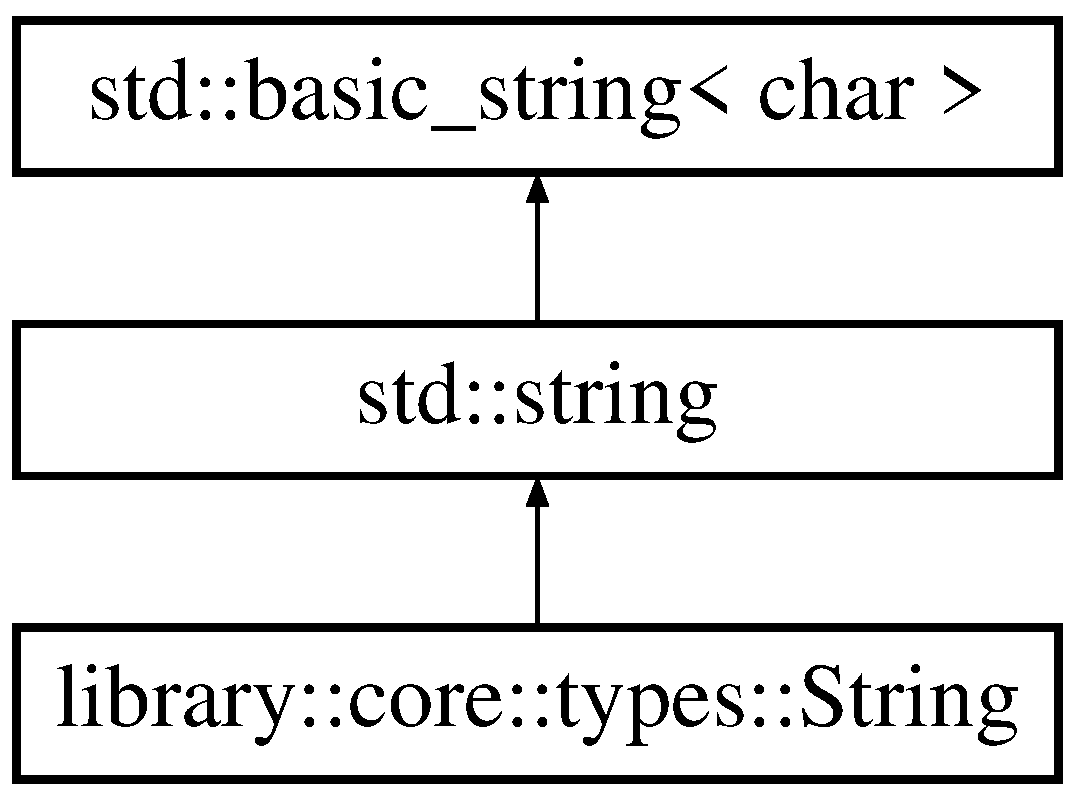
\includegraphics[height=3.000000cm]{classlibrary_1_1core_1_1types_1_1_string}
\end{center}
\end{figure}
\subsection*{Public Member Functions}
\begin{DoxyCompactItemize}
\item 
\hyperlink{classlibrary_1_1core_1_1types_1_1_string_ab49dec039a75f0049c95759141b6d484}{String} ()
\item 
\hyperlink{classlibrary_1_1core_1_1types_1_1_string_a37c737528805786c49eab397ba7b64ae}{String} (const std\+::string \&a\+String)
\item 
\hyperlink{classlibrary_1_1core_1_1types_1_1_string_a97f9b0024a58372a0281b25e2811f3bf}{$\sim$\+String} ()
\item 
bool \hyperlink{classlibrary_1_1core_1_1types_1_1_string_a1981fee5619389b46c786afa7aadc251}{is\+Empty} () const
\item 
bool \hyperlink{classlibrary_1_1core_1_1types_1_1_string_a6d12c373b22a062cfa0270204fc998f5}{is\+Uppercase} () const
\item 
bool \hyperlink{classlibrary_1_1core_1_1types_1_1_string_a3620d335dd5b14029a3a67e75c79be81}{is\+Lowercase} () const
\item 
bool \hyperlink{classlibrary_1_1core_1_1types_1_1_string_abab50e9c0d620b246d0bfde0dad0add5}{match} (const std\+::regex \&a\+Regular\+Expression) const
\begin{DoxyCompactList}\small\item\em Returns whether the string matches a regular expression. \end{DoxyCompactList}\item 
\hyperlink{namespacelibrary_1_1core_1_1types_a701626ea1027888ebbb8cfd0ff7adab0}{Size} \hyperlink{classlibrary_1_1core_1_1types_1_1_string_adc97f82ccc9a3d034bc3127e643199fb}{get\+Length} () const
\item 
char \hyperlink{classlibrary_1_1core_1_1types_1_1_string_ad695264b765448ecf4f8617553012eee}{get\+First} () const
\item 
char \hyperlink{classlibrary_1_1core_1_1types_1_1_string_aae3aaf5e3b3fde3f7b90fd1ee431c9d4}{get\+Last} () const
\item 
\hyperlink{classlibrary_1_1core_1_1types_1_1_string}{String} \hyperlink{classlibrary_1_1core_1_1types_1_1_string_af11475f7a147a11342765a690df18852}{get\+Head} (const \hyperlink{namespacelibrary_1_1core_1_1types_a701626ea1027888ebbb8cfd0ff7adab0}{Size} \&a\+Length) const
\item 
\hyperlink{classlibrary_1_1core_1_1types_1_1_string}{String} \hyperlink{classlibrary_1_1core_1_1types_1_1_string_ac1c579d8fe140ab627b679e1d372746a}{get\+Tail} (const \hyperlink{namespacelibrary_1_1core_1_1types_a701626ea1027888ebbb8cfd0ff7adab0}{Size} \&a\+Length) const
\item 
\hyperlink{classlibrary_1_1core_1_1types_1_1_string}{String} \hyperlink{classlibrary_1_1core_1_1types_1_1_string_aaf9377048b900766d05a1af9182cf251}{get\+Substring} (const \hyperlink{namespacelibrary_1_1core_1_1types_ad87eeb821d7067ec94e06ed1980d6350}{Index} \&a\+Start\+Position, const \hyperlink{namespacelibrary_1_1core_1_1types_a701626ea1027888ebbb8cfd0ff7adab0}{Size} \&a\+Length) const
\item 
\hyperlink{classlibrary_1_1core_1_1types_1_1_string}{String} \& \hyperlink{classlibrary_1_1core_1_1types_1_1_string_a42426ffb11bb0b2789ba0991064a01b5}{trim} ()
\begin{DoxyCompactList}\small\item\em Removes whitespace from both ends. \end{DoxyCompactList}\item 
\hyperlink{classlibrary_1_1core_1_1types_1_1_string}{String} \& \hyperlink{classlibrary_1_1core_1_1types_1_1_string_a8d4100938450cb4c4bba2c3e49d1871d}{replace} (const char a\+Character, const char a\+New\+Character)
\begin{DoxyCompactList}\small\item\em Replace all occurences of character by other character. \end{DoxyCompactList}\item 
\hyperlink{classlibrary_1_1core_1_1types_1_1_string}{String} \& \hyperlink{classlibrary_1_1core_1_1types_1_1_string_a33f558b912c1f24a109e985c3a180f22}{replace} (const \hyperlink{classlibrary_1_1core_1_1types_1_1_string}{String} \&a\+String, const \hyperlink{classlibrary_1_1core_1_1types_1_1_string}{String} \&a\+New\+String)
\begin{DoxyCompactList}\small\item\em Replace all occurences of string by other string. \end{DoxyCompactList}\end{DoxyCompactItemize}
\subsection*{Static Public Member Functions}
\begin{DoxyCompactItemize}
\item 
static \hyperlink{classlibrary_1_1core_1_1types_1_1_string}{String} \hyperlink{classlibrary_1_1core_1_1types_1_1_string_a4d359cb0dba46e14ca46f90e728c2b96}{Empty} ()
\item 
static \hyperlink{classlibrary_1_1core_1_1types_1_1_string}{String} \hyperlink{classlibrary_1_1core_1_1types_1_1_string_afd43951e5c53b89428dc36db99a83842}{Boolean} (bool a\+Boolean)
\item 
static \hyperlink{classlibrary_1_1core_1_1types_1_1_string}{String} \hyperlink{classlibrary_1_1core_1_1types_1_1_string_abbc5a795da1a72d1456ba4950e62602c}{Char} (char a\+Character)
\item 
static \hyperlink{classlibrary_1_1core_1_1types_1_1_string}{String} \hyperlink{classlibrary_1_1core_1_1types_1_1_string_ab476d0986c7d364261ee3e668890836c}{Replicate} (char a\+Character, \hyperlink{namespacelibrary_1_1core_1_1types_a701626ea1027888ebbb8cfd0ff7adab0}{Size} a\+Count)
\item 
static \hyperlink{classlibrary_1_1core_1_1types_1_1_string}{String} \hyperlink{classlibrary_1_1core_1_1types_1_1_string_a85504c430c0fdc58393f819205fedd49}{Replicate} (const \hyperlink{classlibrary_1_1core_1_1types_1_1_string}{String} \&a\+String, \hyperlink{namespacelibrary_1_1core_1_1types_a701626ea1027888ebbb8cfd0ff7adab0}{Size} a\+Count)
\item 
{\footnotesize template$<$typename ... Args$>$ }\\static \hyperlink{classlibrary_1_1core_1_1types_1_1_string}{String} \hyperlink{classlibrary_1_1core_1_1types_1_1_string_ae1745f54be6952d7b5a388239377b287}{Format} (const char $\ast$a\+Format, Args... an\+Argument\+List)
\begin{DoxyCompactList}\small\item\em Create formatted string. \end{DoxyCompactList}\end{DoxyCompactItemize}


\subsection{Detailed Description}
A sequence of characters. 

\begin{DoxyNote}{Note}
The current implementation (derived for std\+::string) is temporary, as this type of inheritance this is not recommended. 
\end{DoxyNote}


\subsection{Constructor \& Destructor Documentation}
\mbox{\Hypertarget{classlibrary_1_1core_1_1types_1_1_string_ab49dec039a75f0049c95759141b6d484}\label{classlibrary_1_1core_1_1types_1_1_string_ab49dec039a75f0049c95759141b6d484}} 
\index{library\+::core\+::types\+::\+String@{library\+::core\+::types\+::\+String}!String@{String}}
\index{String@{String}!library\+::core\+::types\+::\+String@{library\+::core\+::types\+::\+String}}
\subsubsection{\texorpdfstring{String()}{String()}\hspace{0.1cm}{\footnotesize\ttfamily [1/2]}}
{\footnotesize\ttfamily library\+::core\+::types\+::\+String\+::\+String (\begin{DoxyParamCaption}{ }\end{DoxyParamCaption})}

\mbox{\Hypertarget{classlibrary_1_1core_1_1types_1_1_string_a37c737528805786c49eab397ba7b64ae}\label{classlibrary_1_1core_1_1types_1_1_string_a37c737528805786c49eab397ba7b64ae}} 
\index{library\+::core\+::types\+::\+String@{library\+::core\+::types\+::\+String}!String@{String}}
\index{String@{String}!library\+::core\+::types\+::\+String@{library\+::core\+::types\+::\+String}}
\subsubsection{\texorpdfstring{String()}{String()}\hspace{0.1cm}{\footnotesize\ttfamily [2/2]}}
{\footnotesize\ttfamily library\+::core\+::types\+::\+String\+::\+String (\begin{DoxyParamCaption}\item[{const std\+::string \&}]{a\+String }\end{DoxyParamCaption})}

\mbox{\Hypertarget{classlibrary_1_1core_1_1types_1_1_string_a97f9b0024a58372a0281b25e2811f3bf}\label{classlibrary_1_1core_1_1types_1_1_string_a97f9b0024a58372a0281b25e2811f3bf}} 
\index{library\+::core\+::types\+::\+String@{library\+::core\+::types\+::\+String}!````~String@{$\sim$\+String}}
\index{````~String@{$\sim$\+String}!library\+::core\+::types\+::\+String@{library\+::core\+::types\+::\+String}}
\subsubsection{\texorpdfstring{$\sim$\+String()}{~String()}}
{\footnotesize\ttfamily library\+::core\+::types\+::\+String\+::$\sim$\+String (\begin{DoxyParamCaption}{ }\end{DoxyParamCaption})}



\subsection{Member Function Documentation}
\mbox{\Hypertarget{classlibrary_1_1core_1_1types_1_1_string_afd43951e5c53b89428dc36db99a83842}\label{classlibrary_1_1core_1_1types_1_1_string_afd43951e5c53b89428dc36db99a83842}} 
\index{library\+::core\+::types\+::\+String@{library\+::core\+::types\+::\+String}!Boolean@{Boolean}}
\index{Boolean@{Boolean}!library\+::core\+::types\+::\+String@{library\+::core\+::types\+::\+String}}
\subsubsection{\texorpdfstring{Boolean()}{Boolean()}}
{\footnotesize\ttfamily \hyperlink{classlibrary_1_1core_1_1types_1_1_string}{String} library\+::core\+::types\+::\+String\+::\+Boolean (\begin{DoxyParamCaption}\item[{bool}]{a\+Boolean }\end{DoxyParamCaption})\hspace{0.3cm}{\ttfamily [static]}}

\mbox{\Hypertarget{classlibrary_1_1core_1_1types_1_1_string_abbc5a795da1a72d1456ba4950e62602c}\label{classlibrary_1_1core_1_1types_1_1_string_abbc5a795da1a72d1456ba4950e62602c}} 
\index{library\+::core\+::types\+::\+String@{library\+::core\+::types\+::\+String}!Char@{Char}}
\index{Char@{Char}!library\+::core\+::types\+::\+String@{library\+::core\+::types\+::\+String}}
\subsubsection{\texorpdfstring{Char()}{Char()}}
{\footnotesize\ttfamily \hyperlink{classlibrary_1_1core_1_1types_1_1_string}{String} library\+::core\+::types\+::\+String\+::\+Char (\begin{DoxyParamCaption}\item[{char}]{a\+Character }\end{DoxyParamCaption})\hspace{0.3cm}{\ttfamily [static]}}

\mbox{\Hypertarget{classlibrary_1_1core_1_1types_1_1_string_a4d359cb0dba46e14ca46f90e728c2b96}\label{classlibrary_1_1core_1_1types_1_1_string_a4d359cb0dba46e14ca46f90e728c2b96}} 
\index{library\+::core\+::types\+::\+String@{library\+::core\+::types\+::\+String}!Empty@{Empty}}
\index{Empty@{Empty}!library\+::core\+::types\+::\+String@{library\+::core\+::types\+::\+String}}
\subsubsection{\texorpdfstring{Empty()}{Empty()}}
{\footnotesize\ttfamily \hyperlink{classlibrary_1_1core_1_1types_1_1_string}{String} library\+::core\+::types\+::\+String\+::\+Empty (\begin{DoxyParamCaption}{ }\end{DoxyParamCaption})\hspace{0.3cm}{\ttfamily [static]}}

\mbox{\Hypertarget{classlibrary_1_1core_1_1types_1_1_string_ae1745f54be6952d7b5a388239377b287}\label{classlibrary_1_1core_1_1types_1_1_string_ae1745f54be6952d7b5a388239377b287}} 
\index{library\+::core\+::types\+::\+String@{library\+::core\+::types\+::\+String}!Format@{Format}}
\index{Format@{Format}!library\+::core\+::types\+::\+String@{library\+::core\+::types\+::\+String}}
\subsubsection{\texorpdfstring{Format()}{Format()}}
{\footnotesize\ttfamily template$<$typename ... Args$>$ \\
static \hyperlink{classlibrary_1_1core_1_1types_1_1_string}{String} library\+::core\+::types\+::\+String\+::\+Format (\begin{DoxyParamCaption}\item[{const char $\ast$}]{a\+Format,  }\item[{Args...}]{an\+Argument\+List }\end{DoxyParamCaption})\hspace{0.3cm}{\ttfamily [inline]}, {\ttfamily [static]}}



Create formatted string. 


\begin{DoxyCode}
\hyperlink{classlibrary_1_1core_1_1types_1_1_string_ae1745f54be6952d7b5a388239377b287}{String::Format}(\textcolor{stringliteral}{"\{0\}, \{1\}!"}, \textcolor{stringliteral}{"Hello"}, \textcolor{stringliteral}{"World"}) ; \textcolor{comment}{// "Hello, World!"}
\hyperlink{classlibrary_1_1core_1_1types_1_1_string_ae1745f54be6952d7b5a388239377b287}{String::Format}(\textcolor{stringliteral}{"Let's operate \{0\} \{1\}!"}, 123, \textcolor{stringliteral}{"satellites"}) ; \textcolor{comment}{// "Let's operate 123
       satellites!"}
\end{DoxyCode}



\begin{DoxyParams}[1]{Parameters}
\mbox{\tt in}  & {\em a\+Format} & A format \\
\hline
\mbox{\tt in}  & {\em an\+Argument\+List} & A list of arguments \\
\hline
\end{DoxyParams}
\begin{DoxyReturn}{Returns}
Formatted string 
\end{DoxyReturn}
\mbox{\Hypertarget{classlibrary_1_1core_1_1types_1_1_string_ad695264b765448ecf4f8617553012eee}\label{classlibrary_1_1core_1_1types_1_1_string_ad695264b765448ecf4f8617553012eee}} 
\index{library\+::core\+::types\+::\+String@{library\+::core\+::types\+::\+String}!get\+First@{get\+First}}
\index{get\+First@{get\+First}!library\+::core\+::types\+::\+String@{library\+::core\+::types\+::\+String}}
\subsubsection{\texorpdfstring{get\+First()}{getFirst()}}
{\footnotesize\ttfamily char library\+::core\+::types\+::\+String\+::get\+First (\begin{DoxyParamCaption}{ }\end{DoxyParamCaption}) const}

\mbox{\Hypertarget{classlibrary_1_1core_1_1types_1_1_string_af11475f7a147a11342765a690df18852}\label{classlibrary_1_1core_1_1types_1_1_string_af11475f7a147a11342765a690df18852}} 
\index{library\+::core\+::types\+::\+String@{library\+::core\+::types\+::\+String}!get\+Head@{get\+Head}}
\index{get\+Head@{get\+Head}!library\+::core\+::types\+::\+String@{library\+::core\+::types\+::\+String}}
\subsubsection{\texorpdfstring{get\+Head()}{getHead()}}
{\footnotesize\ttfamily \hyperlink{classlibrary_1_1core_1_1types_1_1_string}{String} library\+::core\+::types\+::\+String\+::get\+Head (\begin{DoxyParamCaption}\item[{const \hyperlink{namespacelibrary_1_1core_1_1types_a701626ea1027888ebbb8cfd0ff7adab0}{Size} \&}]{a\+Length }\end{DoxyParamCaption}) const}

\mbox{\Hypertarget{classlibrary_1_1core_1_1types_1_1_string_aae3aaf5e3b3fde3f7b90fd1ee431c9d4}\label{classlibrary_1_1core_1_1types_1_1_string_aae3aaf5e3b3fde3f7b90fd1ee431c9d4}} 
\index{library\+::core\+::types\+::\+String@{library\+::core\+::types\+::\+String}!get\+Last@{get\+Last}}
\index{get\+Last@{get\+Last}!library\+::core\+::types\+::\+String@{library\+::core\+::types\+::\+String}}
\subsubsection{\texorpdfstring{get\+Last()}{getLast()}}
{\footnotesize\ttfamily char library\+::core\+::types\+::\+String\+::get\+Last (\begin{DoxyParamCaption}{ }\end{DoxyParamCaption}) const}

\mbox{\Hypertarget{classlibrary_1_1core_1_1types_1_1_string_adc97f82ccc9a3d034bc3127e643199fb}\label{classlibrary_1_1core_1_1types_1_1_string_adc97f82ccc9a3d034bc3127e643199fb}} 
\index{library\+::core\+::types\+::\+String@{library\+::core\+::types\+::\+String}!get\+Length@{get\+Length}}
\index{get\+Length@{get\+Length}!library\+::core\+::types\+::\+String@{library\+::core\+::types\+::\+String}}
\subsubsection{\texorpdfstring{get\+Length()}{getLength()}}
{\footnotesize\ttfamily \hyperlink{namespacelibrary_1_1core_1_1types_a701626ea1027888ebbb8cfd0ff7adab0}{Size} library\+::core\+::types\+::\+String\+::get\+Length (\begin{DoxyParamCaption}{ }\end{DoxyParamCaption}) const}

\mbox{\Hypertarget{classlibrary_1_1core_1_1types_1_1_string_aaf9377048b900766d05a1af9182cf251}\label{classlibrary_1_1core_1_1types_1_1_string_aaf9377048b900766d05a1af9182cf251}} 
\index{library\+::core\+::types\+::\+String@{library\+::core\+::types\+::\+String}!get\+Substring@{get\+Substring}}
\index{get\+Substring@{get\+Substring}!library\+::core\+::types\+::\+String@{library\+::core\+::types\+::\+String}}
\subsubsection{\texorpdfstring{get\+Substring()}{getSubstring()}}
{\footnotesize\ttfamily \hyperlink{classlibrary_1_1core_1_1types_1_1_string}{String} library\+::core\+::types\+::\+String\+::get\+Substring (\begin{DoxyParamCaption}\item[{const \hyperlink{namespacelibrary_1_1core_1_1types_ad87eeb821d7067ec94e06ed1980d6350}{Index} \&}]{a\+Start\+Position,  }\item[{const \hyperlink{namespacelibrary_1_1core_1_1types_a701626ea1027888ebbb8cfd0ff7adab0}{Size} \&}]{a\+Length }\end{DoxyParamCaption}) const}

\mbox{\Hypertarget{classlibrary_1_1core_1_1types_1_1_string_ac1c579d8fe140ab627b679e1d372746a}\label{classlibrary_1_1core_1_1types_1_1_string_ac1c579d8fe140ab627b679e1d372746a}} 
\index{library\+::core\+::types\+::\+String@{library\+::core\+::types\+::\+String}!get\+Tail@{get\+Tail}}
\index{get\+Tail@{get\+Tail}!library\+::core\+::types\+::\+String@{library\+::core\+::types\+::\+String}}
\subsubsection{\texorpdfstring{get\+Tail()}{getTail()}}
{\footnotesize\ttfamily \hyperlink{classlibrary_1_1core_1_1types_1_1_string}{String} library\+::core\+::types\+::\+String\+::get\+Tail (\begin{DoxyParamCaption}\item[{const \hyperlink{namespacelibrary_1_1core_1_1types_a701626ea1027888ebbb8cfd0ff7adab0}{Size} \&}]{a\+Length }\end{DoxyParamCaption}) const}

\mbox{\Hypertarget{classlibrary_1_1core_1_1types_1_1_string_a1981fee5619389b46c786afa7aadc251}\label{classlibrary_1_1core_1_1types_1_1_string_a1981fee5619389b46c786afa7aadc251}} 
\index{library\+::core\+::types\+::\+String@{library\+::core\+::types\+::\+String}!is\+Empty@{is\+Empty}}
\index{is\+Empty@{is\+Empty}!library\+::core\+::types\+::\+String@{library\+::core\+::types\+::\+String}}
\subsubsection{\texorpdfstring{is\+Empty()}{isEmpty()}}
{\footnotesize\ttfamily bool library\+::core\+::types\+::\+String\+::is\+Empty (\begin{DoxyParamCaption}{ }\end{DoxyParamCaption}) const}

\mbox{\Hypertarget{classlibrary_1_1core_1_1types_1_1_string_a3620d335dd5b14029a3a67e75c79be81}\label{classlibrary_1_1core_1_1types_1_1_string_a3620d335dd5b14029a3a67e75c79be81}} 
\index{library\+::core\+::types\+::\+String@{library\+::core\+::types\+::\+String}!is\+Lowercase@{is\+Lowercase}}
\index{is\+Lowercase@{is\+Lowercase}!library\+::core\+::types\+::\+String@{library\+::core\+::types\+::\+String}}
\subsubsection{\texorpdfstring{is\+Lowercase()}{isLowercase()}}
{\footnotesize\ttfamily bool library\+::core\+::types\+::\+String\+::is\+Lowercase (\begin{DoxyParamCaption}{ }\end{DoxyParamCaption}) const}

\mbox{\Hypertarget{classlibrary_1_1core_1_1types_1_1_string_a6d12c373b22a062cfa0270204fc998f5}\label{classlibrary_1_1core_1_1types_1_1_string_a6d12c373b22a062cfa0270204fc998f5}} 
\index{library\+::core\+::types\+::\+String@{library\+::core\+::types\+::\+String}!is\+Uppercase@{is\+Uppercase}}
\index{is\+Uppercase@{is\+Uppercase}!library\+::core\+::types\+::\+String@{library\+::core\+::types\+::\+String}}
\subsubsection{\texorpdfstring{is\+Uppercase()}{isUppercase()}}
{\footnotesize\ttfamily bool library\+::core\+::types\+::\+String\+::is\+Uppercase (\begin{DoxyParamCaption}{ }\end{DoxyParamCaption}) const}

\mbox{\Hypertarget{classlibrary_1_1core_1_1types_1_1_string_abab50e9c0d620b246d0bfde0dad0add5}\label{classlibrary_1_1core_1_1types_1_1_string_abab50e9c0d620b246d0bfde0dad0add5}} 
\index{library\+::core\+::types\+::\+String@{library\+::core\+::types\+::\+String}!match@{match}}
\index{match@{match}!library\+::core\+::types\+::\+String@{library\+::core\+::types\+::\+String}}
\subsubsection{\texorpdfstring{match()}{match()}}
{\footnotesize\ttfamily bool library\+::core\+::types\+::\+String\+::match (\begin{DoxyParamCaption}\item[{const std\+::regex \&}]{a\+Regular\+Expression }\end{DoxyParamCaption}) const}



Returns whether the string matches a regular expression. 


\begin{DoxyCode}
\hyperlink{classlibrary_1_1core_1_1types_1_1_string_ab49dec039a75f0049c95759141b6d484}{String}(\textcolor{stringliteral}{"abc"}).match(std::regex(\textcolor{stringliteral}{"^[a-z]\{3\}$"})) ; \textcolor{comment}{// True}
\end{DoxyCode}



\begin{DoxyParams}[1]{Parameters}
\mbox{\tt in}  & {\em a\+Regular\+Expression} & A regular expression \\
\hline
\end{DoxyParams}
\begin{DoxyReturn}{Returns}
True if matches regular expression 
\end{DoxyReturn}
\mbox{\Hypertarget{classlibrary_1_1core_1_1types_1_1_string_a8d4100938450cb4c4bba2c3e49d1871d}\label{classlibrary_1_1core_1_1types_1_1_string_a8d4100938450cb4c4bba2c3e49d1871d}} 
\index{library\+::core\+::types\+::\+String@{library\+::core\+::types\+::\+String}!replace@{replace}}
\index{replace@{replace}!library\+::core\+::types\+::\+String@{library\+::core\+::types\+::\+String}}
\subsubsection{\texorpdfstring{replace()}{replace()}\hspace{0.1cm}{\footnotesize\ttfamily [1/2]}}
{\footnotesize\ttfamily \hyperlink{classlibrary_1_1core_1_1types_1_1_string}{String} \& library\+::core\+::types\+::\+String\+::replace (\begin{DoxyParamCaption}\item[{const char}]{a\+Character,  }\item[{const char}]{a\+New\+Character }\end{DoxyParamCaption})}



Replace all occurences of character by other character. 


\begin{DoxyParams}[1]{Parameters}
\mbox{\tt in}  & {\em a\+Character} & A character \\
\hline
\mbox{\tt in}  & {\em a\+New\+Character} & A replacement character \\
\hline
\end{DoxyParams}
\begin{DoxyReturn}{Returns}
Reference to string 
\end{DoxyReturn}
\mbox{\Hypertarget{classlibrary_1_1core_1_1types_1_1_string_a33f558b912c1f24a109e985c3a180f22}\label{classlibrary_1_1core_1_1types_1_1_string_a33f558b912c1f24a109e985c3a180f22}} 
\index{library\+::core\+::types\+::\+String@{library\+::core\+::types\+::\+String}!replace@{replace}}
\index{replace@{replace}!library\+::core\+::types\+::\+String@{library\+::core\+::types\+::\+String}}
\subsubsection{\texorpdfstring{replace()}{replace()}\hspace{0.1cm}{\footnotesize\ttfamily [2/2]}}
{\footnotesize\ttfamily \hyperlink{classlibrary_1_1core_1_1types_1_1_string}{String} \& library\+::core\+::types\+::\+String\+::replace (\begin{DoxyParamCaption}\item[{const \hyperlink{classlibrary_1_1core_1_1types_1_1_string}{String} \&}]{a\+String,  }\item[{const \hyperlink{classlibrary_1_1core_1_1types_1_1_string}{String} \&}]{a\+New\+String }\end{DoxyParamCaption})}



Replace all occurences of string by other string. 


\begin{DoxyParams}[1]{Parameters}
\mbox{\tt in}  & {\em a\+Character} & A string \\
\hline
\mbox{\tt in}  & {\em a\+New\+Character} & A replacement string \\
\hline
\end{DoxyParams}
\begin{DoxyReturn}{Returns}
Reference to string 
\end{DoxyReturn}
\mbox{\Hypertarget{classlibrary_1_1core_1_1types_1_1_string_ab476d0986c7d364261ee3e668890836c}\label{classlibrary_1_1core_1_1types_1_1_string_ab476d0986c7d364261ee3e668890836c}} 
\index{library\+::core\+::types\+::\+String@{library\+::core\+::types\+::\+String}!Replicate@{Replicate}}
\index{Replicate@{Replicate}!library\+::core\+::types\+::\+String@{library\+::core\+::types\+::\+String}}
\subsubsection{\texorpdfstring{Replicate()}{Replicate()}\hspace{0.1cm}{\footnotesize\ttfamily [1/2]}}
{\footnotesize\ttfamily \hyperlink{classlibrary_1_1core_1_1types_1_1_string}{String} library\+::core\+::types\+::\+String\+::\+Replicate (\begin{DoxyParamCaption}\item[{char}]{a\+Character,  }\item[{\hyperlink{namespacelibrary_1_1core_1_1types_a701626ea1027888ebbb8cfd0ff7adab0}{Size}}]{a\+Count }\end{DoxyParamCaption})\hspace{0.3cm}{\ttfamily [static]}}

\mbox{\Hypertarget{classlibrary_1_1core_1_1types_1_1_string_a85504c430c0fdc58393f819205fedd49}\label{classlibrary_1_1core_1_1types_1_1_string_a85504c430c0fdc58393f819205fedd49}} 
\index{library\+::core\+::types\+::\+String@{library\+::core\+::types\+::\+String}!Replicate@{Replicate}}
\index{Replicate@{Replicate}!library\+::core\+::types\+::\+String@{library\+::core\+::types\+::\+String}}
\subsubsection{\texorpdfstring{Replicate()}{Replicate()}\hspace{0.1cm}{\footnotesize\ttfamily [2/2]}}
{\footnotesize\ttfamily \hyperlink{classlibrary_1_1core_1_1types_1_1_string}{String} library\+::core\+::types\+::\+String\+::\+Replicate (\begin{DoxyParamCaption}\item[{const \hyperlink{classlibrary_1_1core_1_1types_1_1_string}{String} \&}]{a\+String,  }\item[{\hyperlink{namespacelibrary_1_1core_1_1types_a701626ea1027888ebbb8cfd0ff7adab0}{Size}}]{a\+Count }\end{DoxyParamCaption})\hspace{0.3cm}{\ttfamily [static]}}

\mbox{\Hypertarget{classlibrary_1_1core_1_1types_1_1_string_a42426ffb11bb0b2789ba0991064a01b5}\label{classlibrary_1_1core_1_1types_1_1_string_a42426ffb11bb0b2789ba0991064a01b5}} 
\index{library\+::core\+::types\+::\+String@{library\+::core\+::types\+::\+String}!trim@{trim}}
\index{trim@{trim}!library\+::core\+::types\+::\+String@{library\+::core\+::types\+::\+String}}
\subsubsection{\texorpdfstring{trim()}{trim()}}
{\footnotesize\ttfamily \hyperlink{classlibrary_1_1core_1_1types_1_1_string}{String} \& library\+::core\+::types\+::\+String\+::trim (\begin{DoxyParamCaption}{ }\end{DoxyParamCaption})}



Removes whitespace from both ends. 

\begin{DoxyReturn}{Returns}
Reference to string 
\end{DoxyReturn}


The documentation for this class was generated from the following files\+:\begin{DoxyCompactItemize}
\item 
include/\+Library/\+Core/\+Types/\hyperlink{_string_8hpp}{String.\+hpp}\item 
src/\+Library/\+Core/\+Types/\hyperlink{_string_8cpp}{String.\+cpp}\end{DoxyCompactItemize}

\hypertarget{classlibrary_1_1core_1_1ctnr_1_1_table}{}\section{library\+:\+:core\+:\+:ctnr\+:\+:Table Class Reference}
\label{classlibrary_1_1core_1_1ctnr_1_1_table}\index{library\+::core\+::ctnr\+::\+Table@{library\+::core\+::ctnr\+::\+Table}}


\hyperlink{classlibrary_1_1core_1_1ctnr_1_1_table}{Table} container.  




{\ttfamily \#include $<$Table.\+hpp$>$}

\subsection*{Public Member Functions}
\begin{DoxyCompactItemize}
\item 
\hyperlink{classlibrary_1_1core_1_1ctnr_1_1_table_a5c88870b3e09883ccaa6e58f26de6b02}{Table} ()=delete
\item 
\hyperlink{classlibrary_1_1core_1_1ctnr_1_1_table_afaaf450a1a4949b48b6290460137921e}{Table} (const \hyperlink{classlibrary_1_1core_1_1ctnr_1_1_table}{Table} \&a\+Table)
\item 
\hyperlink{classlibrary_1_1core_1_1ctnr_1_1_table_a8cdd20d9cd30399a4611b0b8cd2894d5}{$\sim$\+Table} ()
\item 
\hyperlink{classlibrary_1_1core_1_1ctnr_1_1_table}{Table} \& \hyperlink{classlibrary_1_1core_1_1ctnr_1_1_table_af1d446ec74df66da7bd1eb3ff2d6bb55}{operator=} (const \hyperlink{classlibrary_1_1core_1_1ctnr_1_1_table}{Table} \&a\+Table) const
\item 
bool \hyperlink{classlibrary_1_1core_1_1ctnr_1_1_table_af2777d4233cd7caa7cc81b3b957c3a0c}{is\+Defined} () const
\end{DoxyCompactItemize}
\subsection*{Static Public Member Functions}
\begin{DoxyCompactItemize}
\item 
static \hyperlink{classlibrary_1_1core_1_1ctnr_1_1_table}{Table} \hyperlink{classlibrary_1_1core_1_1ctnr_1_1_table_a75089c496f8aac71e374616d55a78e03}{Empty} ()
\end{DoxyCompactItemize}
\subsection*{Friends}
\begin{DoxyCompactItemize}
\item 
std\+::ostream \& \hyperlink{classlibrary_1_1core_1_1ctnr_1_1_table_afaece709b2f143e4011941ae67b7adba}{operator$<$$<$} (std\+::ostream \&an\+Output\+Stream, const \hyperlink{classlibrary_1_1core_1_1ctnr_1_1_table}{Table} \&a\+Table)
\end{DoxyCompactItemize}


\subsection{Detailed Description}
\hyperlink{classlibrary_1_1core_1_1ctnr_1_1_table}{Table} container. 

\subsection{Constructor \& Destructor Documentation}
\mbox{\Hypertarget{classlibrary_1_1core_1_1ctnr_1_1_table_a5c88870b3e09883ccaa6e58f26de6b02}\label{classlibrary_1_1core_1_1ctnr_1_1_table_a5c88870b3e09883ccaa6e58f26de6b02}} 
\index{library\+::core\+::ctnr\+::\+Table@{library\+::core\+::ctnr\+::\+Table}!Table@{Table}}
\index{Table@{Table}!library\+::core\+::ctnr\+::\+Table@{library\+::core\+::ctnr\+::\+Table}}
\subsubsection{\texorpdfstring{Table()}{Table()}\hspace{0.1cm}{\footnotesize\ttfamily [1/2]}}
{\footnotesize\ttfamily library\+::core\+::ctnr\+::\+Table\+::\+Table (\begin{DoxyParamCaption}{ }\end{DoxyParamCaption})\hspace{0.3cm}{\ttfamily [delete]}}

\mbox{\Hypertarget{classlibrary_1_1core_1_1ctnr_1_1_table_afaaf450a1a4949b48b6290460137921e}\label{classlibrary_1_1core_1_1ctnr_1_1_table_afaaf450a1a4949b48b6290460137921e}} 
\index{library\+::core\+::ctnr\+::\+Table@{library\+::core\+::ctnr\+::\+Table}!Table@{Table}}
\index{Table@{Table}!library\+::core\+::ctnr\+::\+Table@{library\+::core\+::ctnr\+::\+Table}}
\subsubsection{\texorpdfstring{Table()}{Table()}\hspace{0.1cm}{\footnotesize\ttfamily [2/2]}}
{\footnotesize\ttfamily library\+::core\+::ctnr\+::\+Table\+::\+Table (\begin{DoxyParamCaption}\item[{const \hyperlink{classlibrary_1_1core_1_1ctnr_1_1_table}{Table} \&}]{a\+Table }\end{DoxyParamCaption})}

\mbox{\Hypertarget{classlibrary_1_1core_1_1ctnr_1_1_table_a8cdd20d9cd30399a4611b0b8cd2894d5}\label{classlibrary_1_1core_1_1ctnr_1_1_table_a8cdd20d9cd30399a4611b0b8cd2894d5}} 
\index{library\+::core\+::ctnr\+::\+Table@{library\+::core\+::ctnr\+::\+Table}!````~Table@{$\sim$\+Table}}
\index{````~Table@{$\sim$\+Table}!library\+::core\+::ctnr\+::\+Table@{library\+::core\+::ctnr\+::\+Table}}
\subsubsection{\texorpdfstring{$\sim$\+Table()}{~Table()}}
{\footnotesize\ttfamily library\+::core\+::ctnr\+::\+Table\+::$\sim$\+Table (\begin{DoxyParamCaption}{ }\end{DoxyParamCaption})}



\subsection{Member Function Documentation}
\mbox{\Hypertarget{classlibrary_1_1core_1_1ctnr_1_1_table_a75089c496f8aac71e374616d55a78e03}\label{classlibrary_1_1core_1_1ctnr_1_1_table_a75089c496f8aac71e374616d55a78e03}} 
\index{library\+::core\+::ctnr\+::\+Table@{library\+::core\+::ctnr\+::\+Table}!Empty@{Empty}}
\index{Empty@{Empty}!library\+::core\+::ctnr\+::\+Table@{library\+::core\+::ctnr\+::\+Table}}
\subsubsection{\texorpdfstring{Empty()}{Empty()}}
{\footnotesize\ttfamily static \hyperlink{classlibrary_1_1core_1_1ctnr_1_1_table}{Table} library\+::core\+::ctnr\+::\+Table\+::\+Empty (\begin{DoxyParamCaption}{ }\end{DoxyParamCaption})\hspace{0.3cm}{\ttfamily [static]}}

\mbox{\Hypertarget{classlibrary_1_1core_1_1ctnr_1_1_table_af2777d4233cd7caa7cc81b3b957c3a0c}\label{classlibrary_1_1core_1_1ctnr_1_1_table_af2777d4233cd7caa7cc81b3b957c3a0c}} 
\index{library\+::core\+::ctnr\+::\+Table@{library\+::core\+::ctnr\+::\+Table}!is\+Defined@{is\+Defined}}
\index{is\+Defined@{is\+Defined}!library\+::core\+::ctnr\+::\+Table@{library\+::core\+::ctnr\+::\+Table}}
\subsubsection{\texorpdfstring{is\+Defined()}{isDefined()}}
{\footnotesize\ttfamily bool library\+::core\+::ctnr\+::\+Table\+::is\+Defined (\begin{DoxyParamCaption}{ }\end{DoxyParamCaption}) const}

\mbox{\Hypertarget{classlibrary_1_1core_1_1ctnr_1_1_table_af1d446ec74df66da7bd1eb3ff2d6bb55}\label{classlibrary_1_1core_1_1ctnr_1_1_table_af1d446ec74df66da7bd1eb3ff2d6bb55}} 
\index{library\+::core\+::ctnr\+::\+Table@{library\+::core\+::ctnr\+::\+Table}!operator=@{operator=}}
\index{operator=@{operator=}!library\+::core\+::ctnr\+::\+Table@{library\+::core\+::ctnr\+::\+Table}}
\subsubsection{\texorpdfstring{operator=()}{operator=()}}
{\footnotesize\ttfamily \hyperlink{classlibrary_1_1core_1_1ctnr_1_1_table}{Table}\& library\+::core\+::ctnr\+::\+Table\+::operator= (\begin{DoxyParamCaption}\item[{const \hyperlink{classlibrary_1_1core_1_1ctnr_1_1_table}{Table} \&}]{a\+Table }\end{DoxyParamCaption}) const}



\subsection{Friends And Related Function Documentation}
\mbox{\Hypertarget{classlibrary_1_1core_1_1ctnr_1_1_table_afaece709b2f143e4011941ae67b7adba}\label{classlibrary_1_1core_1_1ctnr_1_1_table_afaece709b2f143e4011941ae67b7adba}} 
\index{library\+::core\+::ctnr\+::\+Table@{library\+::core\+::ctnr\+::\+Table}!operator$<$$<$@{operator$<$$<$}}
\index{operator$<$$<$@{operator$<$$<$}!library\+::core\+::ctnr\+::\+Table@{library\+::core\+::ctnr\+::\+Table}}
\subsubsection{\texorpdfstring{operator$<$$<$}{operator<<}}
{\footnotesize\ttfamily std\+::ostream\& operator$<$$<$ (\begin{DoxyParamCaption}\item[{std\+::ostream \&}]{an\+Output\+Stream,  }\item[{const \hyperlink{classlibrary_1_1core_1_1ctnr_1_1_table}{Table} \&}]{a\+Table }\end{DoxyParamCaption})\hspace{0.3cm}{\ttfamily [friend]}}



The documentation for this class was generated from the following file\+:\begin{DoxyCompactItemize}
\item 
include/\+Library/\+Core/\+Containers/\hyperlink{_table_8hpp}{Table.\+hpp}\end{DoxyCompactItemize}

\hypertarget{classlibrary_1_1core_1_1error_1_1runtime_1_1_to_be_implemented}{}\section{library\+::core\+::error\+::runtime\+::To\+Be\+Implemented Class Reference}
\label{classlibrary_1_1core_1_1error_1_1runtime_1_1_to_be_implemented}\index{library::core::error::runtime::ToBeImplemented@{library::core::error::runtime::ToBeImplemented}}


To be implemented error class.  




{\ttfamily \#include $<$To\+Be\+Implemented.\+hpp$>$}

Inheritance diagram for library\+::core\+::error\+::runtime\+::To\+Be\+Implemented\+:\begin{figure}[H]
\begin{center}
\leavevmode
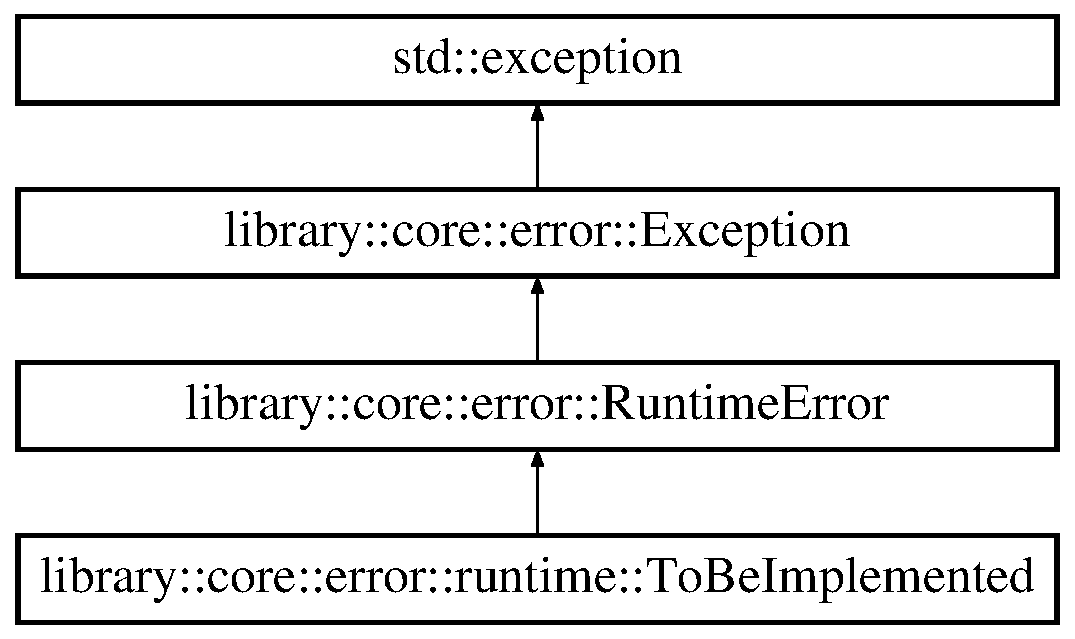
\includegraphics[height=4.000000cm]{classlibrary_1_1core_1_1error_1_1runtime_1_1_to_be_implemented}
\end{center}
\end{figure}
\subsection*{Public Member Functions}
\begin{DoxyCompactItemize}
\item 
\mbox{\hyperlink{classlibrary_1_1core_1_1error_1_1runtime_1_1_to_be_implemented_aa98b3ae5c0ee3329a09b4b03bf27cf85}{To\+Be\+Implemented}} ()
\item 
\mbox{\hyperlink{classlibrary_1_1core_1_1error_1_1runtime_1_1_to_be_implemented_aee7854f221ff5bdade9cb8d67267b6ba}{To\+Be\+Implemented}} (const \mbox{\hyperlink{classlibrary_1_1core_1_1types_1_1_string}{String}} \&a\+Function\+Name)
\item 
\mbox{\hyperlink{classlibrary_1_1core_1_1error_1_1runtime_1_1_to_be_implemented_a4d6d8204b46f1f5eb41458849a891787}{$\sim$\+To\+Be\+Implemented}} ()
\end{DoxyCompactItemize}


\subsection{Detailed Description}
To be implemented error class. 

\subsection{Constructor \& Destructor Documentation}
\mbox{\Hypertarget{classlibrary_1_1core_1_1error_1_1runtime_1_1_to_be_implemented_aa98b3ae5c0ee3329a09b4b03bf27cf85}\label{classlibrary_1_1core_1_1error_1_1runtime_1_1_to_be_implemented_aa98b3ae5c0ee3329a09b4b03bf27cf85}} 
\index{library::core::error::runtime::ToBeImplemented@{library::core::error::runtime::ToBeImplemented}!ToBeImplemented@{ToBeImplemented}}
\index{ToBeImplemented@{ToBeImplemented}!library::core::error::runtime::ToBeImplemented@{library::core::error::runtime::ToBeImplemented}}
\subsubsection{\texorpdfstring{ToBeImplemented()}{ToBeImplemented()}\hspace{0.1cm}{\footnotesize\ttfamily [1/2]}}
{\footnotesize\ttfamily library\+::core\+::error\+::runtime\+::\+To\+Be\+Implemented\+::\+To\+Be\+Implemented (\begin{DoxyParamCaption}{ }\end{DoxyParamCaption})}

\mbox{\Hypertarget{classlibrary_1_1core_1_1error_1_1runtime_1_1_to_be_implemented_aee7854f221ff5bdade9cb8d67267b6ba}\label{classlibrary_1_1core_1_1error_1_1runtime_1_1_to_be_implemented_aee7854f221ff5bdade9cb8d67267b6ba}} 
\index{library::core::error::runtime::ToBeImplemented@{library::core::error::runtime::ToBeImplemented}!ToBeImplemented@{ToBeImplemented}}
\index{ToBeImplemented@{ToBeImplemented}!library::core::error::runtime::ToBeImplemented@{library::core::error::runtime::ToBeImplemented}}
\subsubsection{\texorpdfstring{ToBeImplemented()}{ToBeImplemented()}\hspace{0.1cm}{\footnotesize\ttfamily [2/2]}}
{\footnotesize\ttfamily library\+::core\+::error\+::runtime\+::\+To\+Be\+Implemented\+::\+To\+Be\+Implemented (\begin{DoxyParamCaption}\item[{const \mbox{\hyperlink{classlibrary_1_1core_1_1types_1_1_string}{String}} \&}]{a\+Function\+Name }\end{DoxyParamCaption})}

\mbox{\Hypertarget{classlibrary_1_1core_1_1error_1_1runtime_1_1_to_be_implemented_a4d6d8204b46f1f5eb41458849a891787}\label{classlibrary_1_1core_1_1error_1_1runtime_1_1_to_be_implemented_a4d6d8204b46f1f5eb41458849a891787}} 
\index{library::core::error::runtime::ToBeImplemented@{library::core::error::runtime::ToBeImplemented}!````~ToBeImplemented@{$\sim$ToBeImplemented}}
\index{````~ToBeImplemented@{$\sim$ToBeImplemented}!library::core::error::runtime::ToBeImplemented@{library::core::error::runtime::ToBeImplemented}}
\subsubsection{\texorpdfstring{$\sim$ToBeImplemented()}{~ToBeImplemented()}}
{\footnotesize\ttfamily library\+::core\+::error\+::runtime\+::\+To\+Be\+Implemented\+::$\sim$\+To\+Be\+Implemented (\begin{DoxyParamCaption}{ }\end{DoxyParamCaption})}



The documentation for this class was generated from the following files\+:\begin{DoxyCompactItemize}
\item 
include/\+Library/\+Core/\+Error/\+Runtime/\mbox{\hyperlink{_to_be_implemented_8hpp}{To\+Be\+Implemented.\+hpp}}\item 
src/\+Library/\+Core/\+Error/\+Runtime/\mbox{\hyperlink{_to_be_implemented_8cpp}{To\+Be\+Implemented.\+cpp}}\end{DoxyCompactItemize}

\hypertarget{classlibrary_1_1core_1_1ctnr_1_1_tree}{}\section{library\+:\+:core\+:\+:ctnr\+:\+:Tree Class Reference}
\label{classlibrary_1_1core_1_1ctnr_1_1_tree}\index{library\+::core\+::ctnr\+::\+Tree@{library\+::core\+::ctnr\+::\+Tree}}


Undirected graph in which any two vertices are connected by exactly one path.  




{\ttfamily \#include $<$Tree.\+hpp$>$}

\subsection*{Public Member Functions}
\begin{DoxyCompactItemize}
\item 
\mbox{\Hypertarget{classlibrary_1_1core_1_1ctnr_1_1_tree_ac5fc40b3ef35ab52bc0dbdbf807edb46}\label{classlibrary_1_1core_1_1ctnr_1_1_tree_ac5fc40b3ef35ab52bc0dbdbf807edb46}} 
{\bfseries Tree} (const \hyperlink{classlibrary_1_1core_1_1ctnr_1_1_tree}{Tree} \&a\+Tree)
\item 
\mbox{\Hypertarget{classlibrary_1_1core_1_1ctnr_1_1_tree_a5cc9a5ca245a3d9419caf9f1cd748c9d}\label{classlibrary_1_1core_1_1ctnr_1_1_tree_a5cc9a5ca245a3d9419caf9f1cd748c9d}} 
\hyperlink{classlibrary_1_1core_1_1ctnr_1_1_tree}{Tree} \& {\bfseries operator=} (const \hyperlink{classlibrary_1_1core_1_1ctnr_1_1_tree}{Tree} \&a\+Tree) const
\item 
\mbox{\Hypertarget{classlibrary_1_1core_1_1ctnr_1_1_tree_a7fe044b38601503dca0f2720edead189}\label{classlibrary_1_1core_1_1ctnr_1_1_tree_a7fe044b38601503dca0f2720edead189}} 
bool {\bfseries is\+Defined} () const
\end{DoxyCompactItemize}
\subsection*{Static Public Member Functions}
\begin{DoxyCompactItemize}
\item 
\mbox{\Hypertarget{classlibrary_1_1core_1_1ctnr_1_1_tree_a2ddcc031c7c6e3a97a2dd1ab82231f00}\label{classlibrary_1_1core_1_1ctnr_1_1_tree_a2ddcc031c7c6e3a97a2dd1ab82231f00}} 
static \hyperlink{classlibrary_1_1core_1_1ctnr_1_1_tree}{Tree} {\bfseries Empty} ()
\item 
\mbox{\Hypertarget{classlibrary_1_1core_1_1ctnr_1_1_tree_a5e90e14573c52b7f00233200c76e9e82}\label{classlibrary_1_1core_1_1ctnr_1_1_tree_a5e90e14573c52b7f00233200c76e9e82}} 
static \hyperlink{classlibrary_1_1core_1_1ctnr_1_1_tree}{Tree} {\bfseries Object} (const \hyperlink{classlibrary_1_1core_1_1ctnr_1_1_object}{Object} \&an\+Object)
\end{DoxyCompactItemize}
\subsection*{Friends}
\begin{DoxyCompactItemize}
\item 
\mbox{\Hypertarget{classlibrary_1_1core_1_1ctnr_1_1_tree_aca74cf66509d8f31b83b1c100cb00bea}\label{classlibrary_1_1core_1_1ctnr_1_1_tree_aca74cf66509d8f31b83b1c100cb00bea}} 
std\+::ostream \& {\bfseries operator$<$$<$} (std\+::ostream \&an\+Output\+Stream, const \hyperlink{classlibrary_1_1core_1_1ctnr_1_1_tree}{Tree} \&a\+Tree)
\end{DoxyCompactItemize}


\subsection{Detailed Description}
Undirected graph in which any two vertices are connected by exactly one path. 

A tree data structure can be defined recursively (locally) as a collection of nodes (starting at a root node), where each node is a data structure consisting of a value, together with a list of references to nodes (the \char`\"{}children\char`\"{}), with the constraints that no reference is duplicated, and none points to the root.

https\+://en.wikipedia.\+org/wiki/\+Tree\+\_\+(graph\+\_\+theory) https\+://en.wikipedia.\+org/wiki/\+Tree\+\_\+(data\+\_\+structure) 

The documentation for this class was generated from the following file\+:\begin{DoxyCompactItemize}
\item 
include/\+Library/\+Core/\+Containers/\hyperlink{_tree_8hpp}{Tree.\+hpp}\end{DoxyCompactItemize}

\hypertarget{structlibrary_1_1core_1_1ctnr_1_1_triple}{}\section{library\+:\+:core\+:\+:ctnr\+:\+:Triple$<$ T, U, V $>$ Struct Template Reference}
\label{structlibrary_1_1core_1_1ctnr_1_1_triple}\index{library\+::core\+::ctnr\+::\+Triple$<$ T, U, V $>$@{library\+::core\+::ctnr\+::\+Triple$<$ T, U, V $>$}}


\hyperlink{structlibrary_1_1core_1_1ctnr_1_1_triple}{Triple} container.  




{\ttfamily \#include $<$Triple.\+hpp$>$}

\subsection*{Public Attributes}
\begin{DoxyCompactItemize}
\item 
\mbox{\Hypertarget{structlibrary_1_1core_1_1ctnr_1_1_triple_a620996265dbacc4b8961fcdd4694d1f4}\label{structlibrary_1_1core_1_1ctnr_1_1_triple_a620996265dbacc4b8961fcdd4694d1f4}} 
T {\bfseries first}
\item 
\mbox{\Hypertarget{structlibrary_1_1core_1_1ctnr_1_1_triple_a6727b9eb6453f0db0d0abfcd64dbc87e}\label{structlibrary_1_1core_1_1ctnr_1_1_triple_a6727b9eb6453f0db0d0abfcd64dbc87e}} 
U {\bfseries second}
\item 
\mbox{\Hypertarget{structlibrary_1_1core_1_1ctnr_1_1_triple_a5fdac90c0f2e7a33f2fc5f3fc4dba8e2}\label{structlibrary_1_1core_1_1ctnr_1_1_triple_a5fdac90c0f2e7a33f2fc5f3fc4dba8e2}} 
V {\bfseries third}
\end{DoxyCompactItemize}


\subsection{Detailed Description}
\subsubsection*{template$<$typename T, typename U, typename V$>$\newline
struct library\+::core\+::ctnr\+::\+Triple$<$ T, U, V $>$}

\hyperlink{structlibrary_1_1core_1_1ctnr_1_1_triple}{Triple} container. 

The documentation for this struct was generated from the following file\+:\begin{DoxyCompactItemize}
\item 
include/\+Library/\+Core/\+Containers/\hyperlink{_triple_8hpp}{Triple.\+hpp}\end{DoxyCompactItemize}

\hypertarget{classlibrary_1_1core_1_1error_1_1runtime_1_1_undefined}{}\section{library\+:\+:core\+:\+:error\+:\+:runtime\+:\+:Undefined Class Reference}
\label{classlibrary_1_1core_1_1error_1_1runtime_1_1_undefined}\index{library\+::core\+::error\+::runtime\+::\+Undefined@{library\+::core\+::error\+::runtime\+::\+Undefined}}


\hyperlink{classlibrary_1_1core_1_1error_1_1runtime_1_1_undefined}{Undefined} variable error class.  




{\ttfamily \#include $<$Undefined.\+hpp$>$}

Inheritance diagram for library\+:\+:core\+:\+:error\+:\+:runtime\+:\+:Undefined\+:\begin{figure}[H]
\begin{center}
\leavevmode
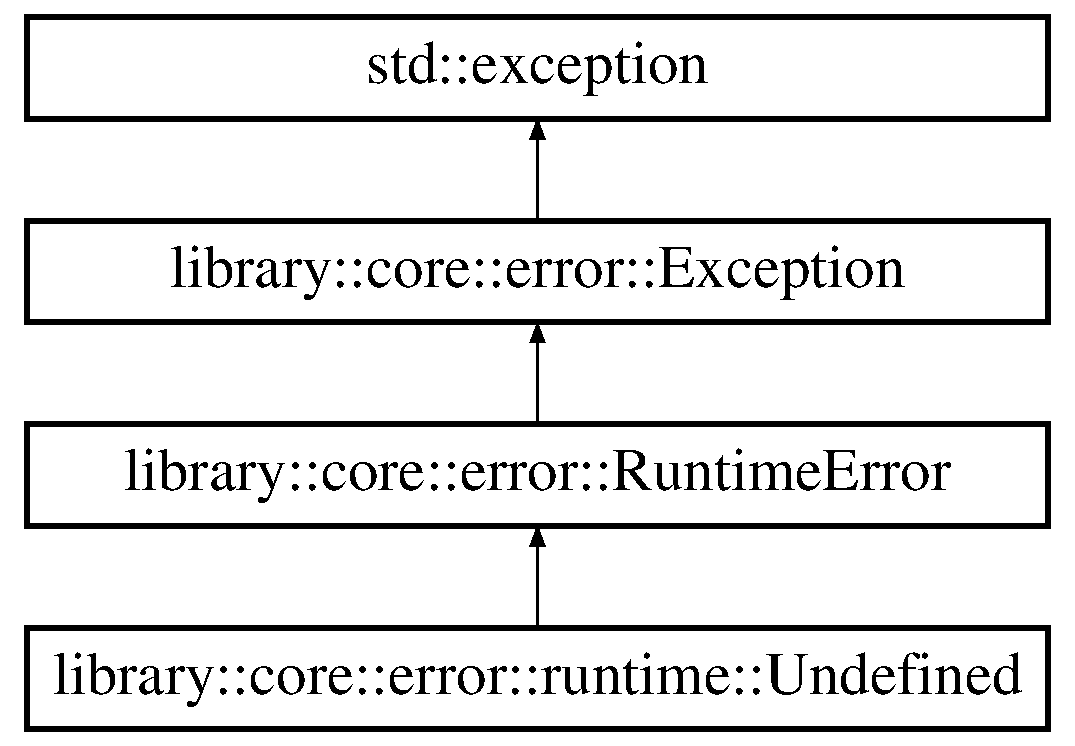
\includegraphics[height=4.000000cm]{classlibrary_1_1core_1_1error_1_1runtime_1_1_undefined}
\end{center}
\end{figure}
\subsection*{Public Member Functions}
\begin{DoxyCompactItemize}
\item 
\hyperlink{classlibrary_1_1core_1_1error_1_1runtime_1_1_undefined_a585cecbe505147926980971fed942b95}{Undefined} (const \hyperlink{classlibrary_1_1core_1_1types_1_1_string}{String} \&a\+Variable\+Name)
\item 
\hyperlink{classlibrary_1_1core_1_1error_1_1runtime_1_1_undefined_a61e341571e36a63bd0894c82b6be7427}{Undefined} (const \hyperlink{classlibrary_1_1core_1_1types_1_1_string}{String} \&a\+Scope, const \hyperlink{classlibrary_1_1core_1_1types_1_1_string}{String} \&a\+Variable\+Name)
\item 
\hyperlink{classlibrary_1_1core_1_1error_1_1runtime_1_1_undefined_a9069574e62bbe7aabab0519b6052cb69}{$\sim$\+Undefined} ()
\end{DoxyCompactItemize}


\subsection{Detailed Description}
\hyperlink{classlibrary_1_1core_1_1error_1_1runtime_1_1_undefined}{Undefined} variable error class. 

\subsection{Constructor \& Destructor Documentation}
\mbox{\Hypertarget{classlibrary_1_1core_1_1error_1_1runtime_1_1_undefined_a585cecbe505147926980971fed942b95}\label{classlibrary_1_1core_1_1error_1_1runtime_1_1_undefined_a585cecbe505147926980971fed942b95}} 
\index{library\+::core\+::error\+::runtime\+::\+Undefined@{library\+::core\+::error\+::runtime\+::\+Undefined}!Undefined@{Undefined}}
\index{Undefined@{Undefined}!library\+::core\+::error\+::runtime\+::\+Undefined@{library\+::core\+::error\+::runtime\+::\+Undefined}}
\subsubsection{\texorpdfstring{Undefined()}{Undefined()}\hspace{0.1cm}{\footnotesize\ttfamily [1/2]}}
{\footnotesize\ttfamily library\+::core\+::error\+::runtime\+::\+Undefined\+::\+Undefined (\begin{DoxyParamCaption}\item[{const \hyperlink{classlibrary_1_1core_1_1types_1_1_string}{String} \&}]{a\+Variable\+Name }\end{DoxyParamCaption})}

\mbox{\Hypertarget{classlibrary_1_1core_1_1error_1_1runtime_1_1_undefined_a61e341571e36a63bd0894c82b6be7427}\label{classlibrary_1_1core_1_1error_1_1runtime_1_1_undefined_a61e341571e36a63bd0894c82b6be7427}} 
\index{library\+::core\+::error\+::runtime\+::\+Undefined@{library\+::core\+::error\+::runtime\+::\+Undefined}!Undefined@{Undefined}}
\index{Undefined@{Undefined}!library\+::core\+::error\+::runtime\+::\+Undefined@{library\+::core\+::error\+::runtime\+::\+Undefined}}
\subsubsection{\texorpdfstring{Undefined()}{Undefined()}\hspace{0.1cm}{\footnotesize\ttfamily [2/2]}}
{\footnotesize\ttfamily library\+::core\+::error\+::runtime\+::\+Undefined\+::\+Undefined (\begin{DoxyParamCaption}\item[{const \hyperlink{classlibrary_1_1core_1_1types_1_1_string}{String} \&}]{a\+Scope,  }\item[{const \hyperlink{classlibrary_1_1core_1_1types_1_1_string}{String} \&}]{a\+Variable\+Name }\end{DoxyParamCaption})}

\mbox{\Hypertarget{classlibrary_1_1core_1_1error_1_1runtime_1_1_undefined_a9069574e62bbe7aabab0519b6052cb69}\label{classlibrary_1_1core_1_1error_1_1runtime_1_1_undefined_a9069574e62bbe7aabab0519b6052cb69}} 
\index{library\+::core\+::error\+::runtime\+::\+Undefined@{library\+::core\+::error\+::runtime\+::\+Undefined}!````~Undefined@{$\sim$\+Undefined}}
\index{````~Undefined@{$\sim$\+Undefined}!library\+::core\+::error\+::runtime\+::\+Undefined@{library\+::core\+::error\+::runtime\+::\+Undefined}}
\subsubsection{\texorpdfstring{$\sim$\+Undefined()}{~Undefined()}}
{\footnotesize\ttfamily library\+::core\+::error\+::runtime\+::\+Undefined\+::$\sim$\+Undefined (\begin{DoxyParamCaption}{ }\end{DoxyParamCaption})}



The documentation for this class was generated from the following files\+:\begin{DoxyCompactItemize}
\item 
include/\+Library/\+Core/\+Error/\+Runtime/\hyperlink{_undefined_8hpp}{Undefined.\+hpp}\item 
src/\+Library/\+Core/\+Error/\+Runtime/\hyperlink{_undefined_8cpp}{Undefined.\+cpp}\end{DoxyCompactItemize}

\hypertarget{classlibrary_1_1core_1_1system_1_1_user}{}\section{library\+:\+:core\+:\+:system\+:\+:User Class Reference}
\label{classlibrary_1_1core_1_1system_1_1_user}\index{library\+::core\+::system\+::\+User@{library\+::core\+::system\+::\+User}}


\hyperlink{classlibrary_1_1core_1_1system_1_1_user}{User}.  




{\ttfamily \#include $<$User.\+hpp$>$}

\subsection*{Public Member Functions}
\begin{DoxyCompactItemize}
\item 
\mbox{\Hypertarget{classlibrary_1_1core_1_1system_1_1_user_af7960468619027fc5a9a19590583c969}\label{classlibrary_1_1core_1_1system_1_1_user_af7960468619027fc5a9a19590583c969}} 
{\bfseries User} (const uint \&a\+U\+ID, const \hyperlink{classlibrary_1_1core_1_1types_1_1_string}{String} \&a\+Name)
\item 
\mbox{\Hypertarget{classlibrary_1_1core_1_1system_1_1_user_a399449d4a49ca4ce9c060e17b0783fc8}\label{classlibrary_1_1core_1_1system_1_1_user_a399449d4a49ca4ce9c060e17b0783fc8}} 
{\bfseries User} (const uint \&a\+U\+ID, const uint \&a\+E\+U\+ID, const \hyperlink{classlibrary_1_1core_1_1types_1_1_string}{String} \&a\+Name)
\item 
\mbox{\Hypertarget{classlibrary_1_1core_1_1system_1_1_user_afffda972cba7158de4f92c150c8256ef}\label{classlibrary_1_1core_1_1system_1_1_user_afffda972cba7158de4f92c150c8256ef}} 
bool {\bfseries operator==} (const \hyperlink{classlibrary_1_1core_1_1system_1_1_user}{User} \&a\+User) const
\item 
\mbox{\Hypertarget{classlibrary_1_1core_1_1system_1_1_user_a666489af790bb3d4773bf2fe8cdaf947}\label{classlibrary_1_1core_1_1system_1_1_user_a666489af790bb3d4773bf2fe8cdaf947}} 
bool {\bfseries operator!=} (const \hyperlink{classlibrary_1_1core_1_1system_1_1_user}{User} \&a\+User) const
\item 
\mbox{\Hypertarget{classlibrary_1_1core_1_1system_1_1_user_aba5006465e6c63c1a8693ad559ca53f1}\label{classlibrary_1_1core_1_1system_1_1_user_aba5006465e6c63c1a8693ad559ca53f1}} 
bool {\bfseries is\+Defined} () const
\item 
\mbox{\Hypertarget{classlibrary_1_1core_1_1system_1_1_user_aafe10eadfc78497c3583badac20982e7}\label{classlibrary_1_1core_1_1system_1_1_user_aafe10eadfc78497c3583badac20982e7}} 
int {\bfseries get\+U\+ID} () const
\item 
\mbox{\Hypertarget{classlibrary_1_1core_1_1system_1_1_user_a57d138f9dc1cd5994ef06f54974f16bc}\label{classlibrary_1_1core_1_1system_1_1_user_a57d138f9dc1cd5994ef06f54974f16bc}} 
int {\bfseries get\+E\+U\+ID} () const
\item 
\mbox{\Hypertarget{classlibrary_1_1core_1_1system_1_1_user_a56ec63ee3e0f1d5bdfd9ab1814350c70}\label{classlibrary_1_1core_1_1system_1_1_user_a56ec63ee3e0f1d5bdfd9ab1814350c70}} 
\hyperlink{classlibrary_1_1core_1_1types_1_1_string}{String} {\bfseries get\+Name} () const
\end{DoxyCompactItemize}
\subsection*{Static Public Member Functions}
\begin{DoxyCompactItemize}
\item 
\mbox{\Hypertarget{classlibrary_1_1core_1_1system_1_1_user_a1195bb2bc30837f9287ea5ed0bfca71b}\label{classlibrary_1_1core_1_1system_1_1_user_a1195bb2bc30837f9287ea5ed0bfca71b}} 
static \hyperlink{classlibrary_1_1core_1_1system_1_1_user}{User} {\bfseries Undefined} ()
\item 
\mbox{\Hypertarget{classlibrary_1_1core_1_1system_1_1_user_a15de974c46bff0ff680403edc4ce129d}\label{classlibrary_1_1core_1_1system_1_1_user_a15de974c46bff0ff680403edc4ce129d}} 
static \hyperlink{classlibrary_1_1core_1_1system_1_1_user}{User} {\bfseries Process} ()
\item 
\mbox{\Hypertarget{classlibrary_1_1core_1_1system_1_1_user_a8843d795dde3c3f0b2054b83a7124830}\label{classlibrary_1_1core_1_1system_1_1_user_a8843d795dde3c3f0b2054b83a7124830}} 
static \hyperlink{classlibrary_1_1core_1_1system_1_1_user}{User} {\bfseries U\+ID} (const uint \&a\+U\+ID)
\item 
\mbox{\Hypertarget{classlibrary_1_1core_1_1system_1_1_user_a2088b7516e89adf5b6fc9f13e58acc61}\label{classlibrary_1_1core_1_1system_1_1_user_a2088b7516e89adf5b6fc9f13e58acc61}} 
static \hyperlink{classlibrary_1_1core_1_1system_1_1_user}{User} {\bfseries Name} (const \hyperlink{classlibrary_1_1core_1_1types_1_1_string}{String} \&a\+Name)
\end{DoxyCompactItemize}
\subsection*{Friends}
\begin{DoxyCompactItemize}
\item 
\mbox{\Hypertarget{classlibrary_1_1core_1_1system_1_1_user_ac434498b36c6e29a86acbb50589e91a3}\label{classlibrary_1_1core_1_1system_1_1_user_ac434498b36c6e29a86acbb50589e91a3}} 
std\+::ostream \& {\bfseries operator$<$$<$} (std\+::ostream \&an\+Output\+Stream, const \hyperlink{classlibrary_1_1core_1_1system_1_1_user}{User} \&a\+User)
\end{DoxyCompactItemize}


\subsection{Detailed Description}
\hyperlink{classlibrary_1_1core_1_1system_1_1_user}{User}. 

P\+O\+S\+IX compliant

https\+://en.wikipedia.\+org/wiki/\+User\+\_\+identifier 

The documentation for this class was generated from the following file\+:\begin{DoxyCompactItemize}
\item 
include/\+Library/\+Core/\+System/\hyperlink{_user_8hpp}{User.\+hpp}\end{DoxyCompactItemize}

\hypertarget{classlibrary_1_1core_1_1error_1_1runtime_1_1_wrong}{}\section{library\+::core\+::error\+::runtime\+::Wrong Class Reference}
\label{classlibrary_1_1core_1_1error_1_1runtime_1_1_wrong}\index{library::core::error::runtime::Wrong@{library::core::error::runtime::Wrong}}


\mbox{\hyperlink{classlibrary_1_1core_1_1error_1_1runtime_1_1_wrong}{Wrong}} variable error class.  




{\ttfamily \#include $<$Wrong.\+hpp$>$}

Inheritance diagram for library\+::core\+::error\+::runtime\+::Wrong\+:\begin{figure}[H]
\begin{center}
\leavevmode
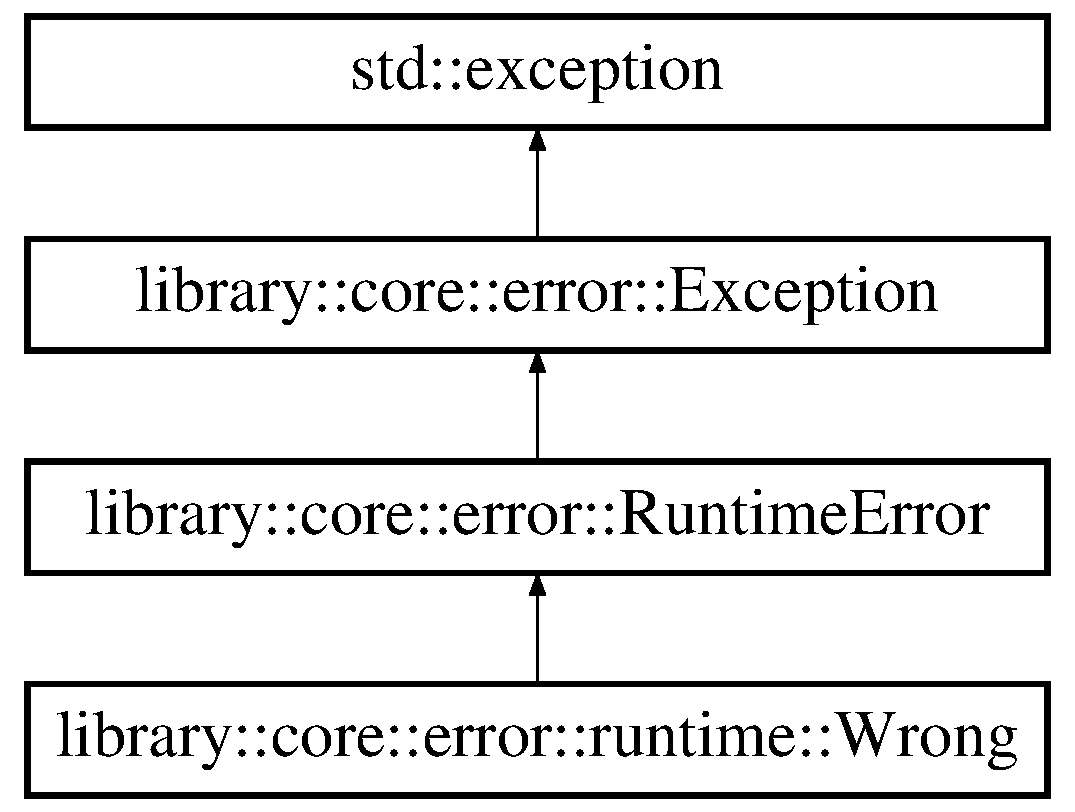
\includegraphics[height=4.000000cm]{classlibrary_1_1core_1_1error_1_1runtime_1_1_wrong}
\end{center}
\end{figure}
\subsection*{Public Member Functions}
\begin{DoxyCompactItemize}
\item 
\mbox{\hyperlink{classlibrary_1_1core_1_1error_1_1runtime_1_1_wrong_acb341a0822b64bfa2d8cdf7963b24f96}{Wrong}} (const \mbox{\hyperlink{classlibrary_1_1core_1_1types_1_1_string}{String}} \&a\+Variable\+Name)
\item 
{\footnotesize template$<$typename ... Args$>$ }\\\mbox{\hyperlink{classlibrary_1_1core_1_1error_1_1runtime_1_1_wrong_a136f670283ce244b5db8be988db73a73}{Wrong}} (const \mbox{\hyperlink{classlibrary_1_1core_1_1types_1_1_string}{String}} \&a\+Variable\+Name, Args... an\+Argument\+List)
\item 
\mbox{\hyperlink{classlibrary_1_1core_1_1error_1_1runtime_1_1_wrong_a6cdcfe31f32807b295695b9bd288d1cf}{$\sim$\+Wrong}} ()
\end{DoxyCompactItemize}


\subsection{Detailed Description}
\mbox{\hyperlink{classlibrary_1_1core_1_1error_1_1runtime_1_1_wrong}{Wrong}} variable error class. 

\subsection{Constructor \& Destructor Documentation}
\mbox{\Hypertarget{classlibrary_1_1core_1_1error_1_1runtime_1_1_wrong_acb341a0822b64bfa2d8cdf7963b24f96}\label{classlibrary_1_1core_1_1error_1_1runtime_1_1_wrong_acb341a0822b64bfa2d8cdf7963b24f96}} 
\index{library::core::error::runtime::Wrong@{library::core::error::runtime::Wrong}!Wrong@{Wrong}}
\index{Wrong@{Wrong}!library::core::error::runtime::Wrong@{library::core::error::runtime::Wrong}}
\subsubsection{\texorpdfstring{Wrong()}{Wrong()}\hspace{0.1cm}{\footnotesize\ttfamily [1/2]}}
{\footnotesize\ttfamily library\+::core\+::error\+::runtime\+::\+Wrong\+::\+Wrong (\begin{DoxyParamCaption}\item[{const \mbox{\hyperlink{classlibrary_1_1core_1_1types_1_1_string}{String}} \&}]{a\+Variable\+Name }\end{DoxyParamCaption})}

\mbox{\Hypertarget{classlibrary_1_1core_1_1error_1_1runtime_1_1_wrong_a136f670283ce244b5db8be988db73a73}\label{classlibrary_1_1core_1_1error_1_1runtime_1_1_wrong_a136f670283ce244b5db8be988db73a73}} 
\index{library::core::error::runtime::Wrong@{library::core::error::runtime::Wrong}!Wrong@{Wrong}}
\index{Wrong@{Wrong}!library::core::error::runtime::Wrong@{library::core::error::runtime::Wrong}}
\subsubsection{\texorpdfstring{Wrong()}{Wrong()}\hspace{0.1cm}{\footnotesize\ttfamily [2/2]}}
{\footnotesize\ttfamily template$<$typename ... Args$>$ \\
library\+::core\+::error\+::runtime\+::\+Wrong\+::\+Wrong (\begin{DoxyParamCaption}\item[{const \mbox{\hyperlink{classlibrary_1_1core_1_1types_1_1_string}{String}} \&}]{a\+Variable\+Name,  }\item[{Args...}]{an\+Argument\+List }\end{DoxyParamCaption})\hspace{0.3cm}{\ttfamily [inline]}}

\mbox{\Hypertarget{classlibrary_1_1core_1_1error_1_1runtime_1_1_wrong_a6cdcfe31f32807b295695b9bd288d1cf}\label{classlibrary_1_1core_1_1error_1_1runtime_1_1_wrong_a6cdcfe31f32807b295695b9bd288d1cf}} 
\index{library::core::error::runtime::Wrong@{library::core::error::runtime::Wrong}!````~Wrong@{$\sim$Wrong}}
\index{````~Wrong@{$\sim$Wrong}!library::core::error::runtime::Wrong@{library::core::error::runtime::Wrong}}
\subsubsection{\texorpdfstring{$\sim$Wrong()}{~Wrong()}}
{\footnotesize\ttfamily library\+::core\+::error\+::runtime\+::\+Wrong\+::$\sim$\+Wrong (\begin{DoxyParamCaption}{ }\end{DoxyParamCaption})}



The documentation for this class was generated from the following files\+:\begin{DoxyCompactItemize}
\item 
include/\+Library/\+Core/\+Error/\+Runtime/\mbox{\hyperlink{_wrong_8hpp}{Wrong.\+hpp}}\item 
src/\+Library/\+Core/\+Error/\+Runtime/\mbox{\hyperlink{_wrong_8cpp}{Wrong.\+cpp}}\end{DoxyCompactItemize}

\hypertarget{classlibrary_1_1core_1_1ctnr_1_1iterators_1_1_zip_iterator}{}\section{library\+:\+:core\+:\+:ctnr\+:\+:iterators\+:\+:Zip\+Iterator$<$ T $>$ Class Template Reference}
\label{classlibrary_1_1core_1_1ctnr_1_1iterators_1_1_zip_iterator}\index{library\+::core\+::ctnr\+::iterators\+::\+Zip\+Iterator$<$ T $>$@{library\+::core\+::ctnr\+::iterators\+::\+Zip\+Iterator$<$ T $>$}}


Zip iterator.  




{\ttfamily \#include $<$Zip.\+hpp$>$}

\subsection*{Classes}
\begin{DoxyCompactItemize}
\item 
class \hyperlink{classlibrary_1_1core_1_1ctnr_1_1iterators_1_1_zip_iterator_1_1_iterator}{Iterator}
\end{DoxyCompactItemize}
\subsection*{Public Member Functions}
\begin{DoxyCompactItemize}
\item 
\hyperlink{classlibrary_1_1core_1_1ctnr_1_1iterators_1_1_zip_iterator_a3d8960d14f07cf22a2de2994eabe46aa}{Zip\+Iterator} (T \&... a\+Sequence)
\item 
\hyperlink{classlibrary_1_1core_1_1ctnr_1_1iterators_1_1_zip_iterator_1_1_iterator}{Zip\+Iterator\+::\+Iterator} \hyperlink{classlibrary_1_1core_1_1ctnr_1_1iterators_1_1_zip_iterator_a0467e25b565ac7b73b22a7002b87d189}{begin} () const
\item 
\hyperlink{classlibrary_1_1core_1_1ctnr_1_1iterators_1_1_zip_iterator_1_1_iterator}{Zip\+Iterator\+::\+Iterator} \hyperlink{classlibrary_1_1core_1_1ctnr_1_1iterators_1_1_zip_iterator_a91c3191909df9dcc737f14d9e38d9a78}{end} () const
\end{DoxyCompactItemize}


\subsection{Detailed Description}
\subsubsection*{template$<$typename... T$>$\newline
class library\+::core\+::ctnr\+::iterators\+::\+Zip\+Iterator$<$ T $>$}

Zip iterator. 

https\+://gist.github.\+com/mortehu/373069390c75b02f98b655e3f7dbef9a 

\subsection{Constructor \& Destructor Documentation}
\mbox{\Hypertarget{classlibrary_1_1core_1_1ctnr_1_1iterators_1_1_zip_iterator_a3d8960d14f07cf22a2de2994eabe46aa}\label{classlibrary_1_1core_1_1ctnr_1_1iterators_1_1_zip_iterator_a3d8960d14f07cf22a2de2994eabe46aa}} 
\index{library\+::core\+::ctnr\+::iterators\+::\+Zip\+Iterator@{library\+::core\+::ctnr\+::iterators\+::\+Zip\+Iterator}!Zip\+Iterator@{Zip\+Iterator}}
\index{Zip\+Iterator@{Zip\+Iterator}!library\+::core\+::ctnr\+::iterators\+::\+Zip\+Iterator@{library\+::core\+::ctnr\+::iterators\+::\+Zip\+Iterator}}
\subsubsection{\texorpdfstring{Zip\+Iterator()}{ZipIterator()}}
{\footnotesize\ttfamily template$<$typename... T$>$ \\
\hyperlink{classlibrary_1_1core_1_1ctnr_1_1iterators_1_1_zip_iterator}{library\+::core\+::ctnr\+::iterators\+::\+Zip\+Iterator}$<$ T $>$\+::\hyperlink{classlibrary_1_1core_1_1ctnr_1_1iterators_1_1_zip_iterator}{Zip\+Iterator} (\begin{DoxyParamCaption}\item[{T \&...}]{a\+Sequence }\end{DoxyParamCaption})\hspace{0.3cm}{\ttfamily [inline]}}



\subsection{Member Function Documentation}
\mbox{\Hypertarget{classlibrary_1_1core_1_1ctnr_1_1iterators_1_1_zip_iterator_a0467e25b565ac7b73b22a7002b87d189}\label{classlibrary_1_1core_1_1ctnr_1_1iterators_1_1_zip_iterator_a0467e25b565ac7b73b22a7002b87d189}} 
\index{library\+::core\+::ctnr\+::iterators\+::\+Zip\+Iterator@{library\+::core\+::ctnr\+::iterators\+::\+Zip\+Iterator}!begin@{begin}}
\index{begin@{begin}!library\+::core\+::ctnr\+::iterators\+::\+Zip\+Iterator@{library\+::core\+::ctnr\+::iterators\+::\+Zip\+Iterator}}
\subsubsection{\texorpdfstring{begin()}{begin()}}
{\footnotesize\ttfamily template$<$typename... T$>$ \\
\hyperlink{classlibrary_1_1core_1_1ctnr_1_1iterators_1_1_zip_iterator_1_1_iterator}{Zip\+Iterator\+::\+Iterator} \hyperlink{classlibrary_1_1core_1_1ctnr_1_1iterators_1_1_zip_iterator}{library\+::core\+::ctnr\+::iterators\+::\+Zip\+Iterator}$<$ T $>$\+::begin (\begin{DoxyParamCaption}{ }\end{DoxyParamCaption}) const\hspace{0.3cm}{\ttfamily [inline]}}

\mbox{\Hypertarget{classlibrary_1_1core_1_1ctnr_1_1iterators_1_1_zip_iterator_a91c3191909df9dcc737f14d9e38d9a78}\label{classlibrary_1_1core_1_1ctnr_1_1iterators_1_1_zip_iterator_a91c3191909df9dcc737f14d9e38d9a78}} 
\index{library\+::core\+::ctnr\+::iterators\+::\+Zip\+Iterator@{library\+::core\+::ctnr\+::iterators\+::\+Zip\+Iterator}!end@{end}}
\index{end@{end}!library\+::core\+::ctnr\+::iterators\+::\+Zip\+Iterator@{library\+::core\+::ctnr\+::iterators\+::\+Zip\+Iterator}}
\subsubsection{\texorpdfstring{end()}{end()}}
{\footnotesize\ttfamily template$<$typename... T$>$ \\
\hyperlink{classlibrary_1_1core_1_1ctnr_1_1iterators_1_1_zip_iterator_1_1_iterator}{Zip\+Iterator\+::\+Iterator} \hyperlink{classlibrary_1_1core_1_1ctnr_1_1iterators_1_1_zip_iterator}{library\+::core\+::ctnr\+::iterators\+::\+Zip\+Iterator}$<$ T $>$\+::end (\begin{DoxyParamCaption}{ }\end{DoxyParamCaption}) const\hspace{0.3cm}{\ttfamily [inline]}}



The documentation for this class was generated from the following file\+:\begin{DoxyCompactItemize}
\item 
include/\+Library/\+Core/\+Containers/\+Iterators/\hyperlink{_zip_8hpp}{Zip.\+hpp}\end{DoxyCompactItemize}

\chapter{File Documentation}
\hypertarget{_c_o_n_t_r_i_b_u_t_i_n_g_8md}{}\section{C\+O\+N\+T\+R\+I\+B\+U\+T\+I\+N\+G.\+md File Reference}
\label{_c_o_n_t_r_i_b_u_t_i_n_g_8md}\index{CONTRIBUTING.md@{CONTRIBUTING.md}}

\hypertarget{_tutorial_8md}{}\section{docs/\+Tutorial.md File Reference}
\label{_tutorial_8md}\index{docs/Tutorial.md@{docs/Tutorial.md}}

\hypertarget{_array_8hpp}{}\section{include/\+Library/\+Core/\+Containers/\+Array.hpp File Reference}
\label{_array_8hpp}\index{include/\+Library/\+Core/\+Containers/\+Array.\+hpp@{include/\+Library/\+Core/\+Containers/\+Array.\+hpp}}
{\ttfamily \#include $<$Library/\+Core/\+Types/\+Index.\+hpp$>$}\newline
{\ttfamily \#include $<$Library/\+Core/\+Types/\+Size.\+hpp$>$}\newline
{\ttfamily \#include $<$Library/\+Core/\+Types/\+String.\+hpp$>$}\newline
{\ttfamily \#include $<$functional$>$}\newline
{\ttfamily \#include $<$vector$>$}\newline
{\ttfamily \#include $<$ostream$>$}\newline
{\ttfamily \#include $<$Library/\+Core/\+Containers/\+Array.\+tpp$>$}\newline
\subsection*{Classes}
\begin{DoxyCompactItemize}
\item 
class \hyperlink{classlibrary_1_1core_1_1ctnr_1_1_array}{library\+::core\+::ctnr\+::\+Array$<$ T $>$}
\begin{DoxyCompactList}\small\item\em \hyperlink{classlibrary_1_1core_1_1ctnr_1_1_array}{Array} container. \end{DoxyCompactList}\end{DoxyCompactItemize}
\subsection*{Namespaces}
\begin{DoxyCompactItemize}
\item 
 \hyperlink{namespacelibrary}{library}
\item 
 \hyperlink{namespacelibrary_1_1core}{library\+::core}
\item 
 \hyperlink{namespacelibrary_1_1core_1_1ctnr}{library\+::core\+::ctnr}
\end{DoxyCompactItemize}


\subsection{Detailed Description}
Library/\+Core

\begin{DoxyAuthor}{Author}
Lucas Brémond \href{mailto:lucas@loftorbital.com}{\tt lucas@loftorbital.\+com}  T\+BD 
\end{DoxyAuthor}

\hypertarget{_dictionary_8hpp}{}\section{include/\+Library/\+Core/\+Containers/\+Dictionary.hpp File Reference}
\label{_dictionary_8hpp}\index{include/\+Library/\+Core/\+Containers/\+Dictionary.\+hpp@{include/\+Library/\+Core/\+Containers/\+Dictionary.\+hpp}}
{\ttfamily \#include $<$Library/\+Core/\+File\+System/\+File.\+hpp$>$}\newline
{\ttfamily \#include $<$Library/\+Core/\+Containers/\+List.\+hpp$>$}\newline
{\ttfamily \#include $<$Library/\+Core/\+Containers/\+Ordered\+Map.\+hpp$>$}\newline
{\ttfamily \#include $<$Library/\+Core/\+Types/\+String.\+hpp$>$}\newline
{\ttfamily \#include $<$Library/\+Core/\+Types/\+Size.\+hpp$>$}\newline
{\ttfamily \#include $<$Library/\+Core/\+Containers/\+Object.\+hpp$>$}\newline
\subsection*{Classes}
\begin{DoxyCompactItemize}
\item 
class \hyperlink{classlibrary_1_1core_1_1ctnr_1_1_dictionary}{library\+::core\+::ctnr\+::\+Dictionary}
\begin{DoxyCompactList}\small\item\em Key-\/value pairs container. \end{DoxyCompactList}\item 
class \hyperlink{classlibrary_1_1core_1_1ctnr_1_1_dictionary_1_1_iterator}{library\+::core\+::ctnr\+::\+Dictionary\+::\+Iterator}
\item 
class \hyperlink{classlibrary_1_1core_1_1ctnr_1_1_dictionary_1_1_const_iterator}{library\+::core\+::ctnr\+::\+Dictionary\+::\+Const\+Iterator}
\end{DoxyCompactItemize}
\subsection*{Namespaces}
\begin{DoxyCompactItemize}
\item 
 \hyperlink{namespacelibrary}{library}
\item 
 \hyperlink{namespacelibrary_1_1core}{library\+::core}
\item 
 \hyperlink{namespacelibrary_1_1core_1_1ctnr}{library\+::core\+::ctnr}
\end{DoxyCompactItemize}


\subsection{Detailed Description}
Library/\+Core

\begin{DoxyAuthor}{Author}
Lucas Brémond \href{mailto:lucas@loftorbital.com}{\tt lucas@loftorbital.\+com}  T\+BD 
\end{DoxyAuthor}

\hypertarget{_graph_8hpp}{}\section{include/\+Library/\+Core/\+Containers/\+Graph.hpp File Reference}
\label{_graph_8hpp}\index{include/Library/Core/Containers/Graph.hpp@{include/Library/Core/Containers/Graph.hpp}}
\subsection*{Classes}
\begin{DoxyCompactItemize}
\item 
class \mbox{\hyperlink{classlibrary_1_1core_1_1ctnr_1_1_graph}{library\+::core\+::ctnr\+::\+Graph}}
\begin{DoxyCompactList}\small\item\em Structure consisting of a finite set of vertices, together with a set of pairs of these vertices (edges). \end{DoxyCompactList}\end{DoxyCompactItemize}
\subsection*{Namespaces}
\begin{DoxyCompactItemize}
\item 
 \mbox{\hyperlink{namespacelibrary}{library}}
\item 
 \mbox{\hyperlink{namespacelibrary_1_1core}{library\+::core}}
\item 
 \mbox{\hyperlink{namespacelibrary_1_1core_1_1ctnr}{library\+::core\+::ctnr}}
\end{DoxyCompactItemize}


\subsection{Detailed Description}
@project Library ▸ Core

\begin{DoxyAuthor}{Author}
Lucas Brémond \href{mailto:lucas@loftorbital.com}{\texttt{ lucas@loftorbital.\+com}} @license Apache License 2.\+0 
\end{DoxyAuthor}

\hypertarget{_zip_8hpp}{}\section{include/\+Library/\+Core/\+Containers/\+Iterators/\+Zip.hpp File Reference}
\label{_zip_8hpp}\index{include/\+Library/\+Core/\+Containers/\+Iterators/\+Zip.\+hpp@{include/\+Library/\+Core/\+Containers/\+Iterators/\+Zip.\+hpp}}
{\ttfamily \#include $<$iterator$>$}\newline
{\ttfamily \#include $<$tuple$>$}\newline
{\ttfamily \#include $<$utility$>$}\newline
\subsection*{Classes}
\begin{DoxyCompactItemize}
\item 
class \hyperlink{classlibrary_1_1core_1_1ctnr_1_1iterators_1_1_zip_iterator}{library\+::core\+::ctnr\+::iterators\+::\+Zip\+Iterator$<$ T $>$}
\begin{DoxyCompactList}\small\item\em Zip iterator. \end{DoxyCompactList}\item 
class \hyperlink{classlibrary_1_1core_1_1ctnr_1_1iterators_1_1_zip_iterator_1_1_iterator}{library\+::core\+::ctnr\+::iterators\+::\+Zip\+Iterator$<$ T $>$\+::\+Iterator}
\end{DoxyCompactItemize}
\subsection*{Namespaces}
\begin{DoxyCompactItemize}
\item 
 \hyperlink{namespacelibrary}{library}
\item 
 \hyperlink{namespacelibrary_1_1core}{library\+::core}
\item 
 \hyperlink{namespacelibrary_1_1core_1_1ctnr}{library\+::core\+::ctnr}
\item 
 \hyperlink{namespacelibrary_1_1core_1_1ctnr_1_1iterators}{library\+::core\+::ctnr\+::iterators}
\end{DoxyCompactItemize}
\subsection*{Functions}
\begin{DoxyCompactItemize}
\item 
{\footnotesize template$<$typename... T$>$ }\\auto \hyperlink{namespacelibrary_1_1core_1_1ctnr_1_1iterators_a42406e4b2d99c4ff14d1412f15674788}{library\+::core\+::ctnr\+::iterators\+::\+Zip} (T \&\&... seqs)
\end{DoxyCompactItemize}


\subsection{Detailed Description}
Library/\+Core

\begin{DoxyAuthor}{Author}
Lucas Brémond \href{mailto:lucas@loftorbital.com}{\tt lucas@loftorbital.\+com}  Apache License 2.\+0 
\end{DoxyAuthor}

\hypertarget{_list_8hpp}{}\section{include/\+Library/\+Core/\+Containers/\+List.hpp File Reference}
\label{_list_8hpp}\index{include/\+Library/\+Core/\+Containers/\+List.\+hpp@{include/\+Library/\+Core/\+Containers/\+List.\+hpp}}
{\ttfamily \#include $<$list$>$}\newline
\subsection*{Typedefs}
\begin{DoxyCompactItemize}
\item 
\mbox{\Hypertarget{_list_8hpp_a87ccf40619002299b341a5e76e989912}\label{_list_8hpp_a87ccf40619002299b341a5e76e989912}} 
{\footnotesize template$<$class T $>$ }\\using \hyperlink{_list_8hpp_a87ccf40619002299b341a5e76e989912}{library\+::core\+::ctnr\+::\+List} = std\+::list$<$ T $>$
\begin{DoxyCompactList}\small\item\em List container. \end{DoxyCompactList}\end{DoxyCompactItemize}


\subsection{Detailed Description}
Library/\+Core

\begin{DoxyAuthor}{Author}
Lucas Brémond \href{mailto:lucas@loftorbital.com}{\tt lucas@loftorbital.\+com}  T\+BD 
\end{DoxyAuthor}

\hypertarget{_map_8hpp}{}\section{include/\+Library/\+Core/\+Containers/\+Map.hpp File Reference}
\label{_map_8hpp}\index{include/Library/Core/Containers/Map.hpp@{include/Library/Core/Containers/Map.hpp}}
{\ttfamily \#include $<$map$>$}\newline
\subsection*{Namespaces}
\begin{DoxyCompactItemize}
\item 
 \mbox{\hyperlink{namespacelibrary}{library}}
\item 
 \mbox{\hyperlink{namespacelibrary_1_1core}{library\+::core}}
\item 
 \mbox{\hyperlink{namespacelibrary_1_1core_1_1ctnr}{library\+::core\+::ctnr}}
\end{DoxyCompactItemize}
\subsection*{Typedefs}
\begin{DoxyCompactItemize}
\item 
{\footnotesize template$<$class Key , class T , class Compare  = std\+::less$<$\+Key$>$, class Allocator  = std\+::allocator$<$std\+::pair$<$const Key, T$>$$>$$>$ }\\using \mbox{\hyperlink{namespacelibrary_1_1core_1_1ctnr_a248e088a0b4ec44aff451a5c3663dcee}{library\+::core\+::ctnr\+::\+Map}} = std\+::map$<$ Key, T, Compare, Allocator $>$
\begin{DoxyCompactList}\small\item\em Map container. \end{DoxyCompactList}\end{DoxyCompactItemize}


\subsection{Detailed Description}
@project Library ▸ Core

\begin{DoxyAuthor}{Author}
Lucas Brémond \href{mailto:lucas@loftorbital.com}{\texttt{ lucas@loftorbital.\+com}} @license Apache License 2.\+0 
\end{DoxyAuthor}

\hypertarget{_object_8hpp}{}\section{include/\+Library/\+Core/\+Containers/\+Object.hpp File Reference}
\label{_object_8hpp}\index{include/Library/Core/Containers/Object.hpp@{include/Library/Core/Containers/Object.hpp}}
{\ttfamily \#include $<$Library/\+Core/\+File\+System/\+File.\+hpp$>$}\newline
{\ttfamily \#include $<$Library/\+Core/\+Containers/\+Array.\+hpp$>$}\newline
{\ttfamily \#include $<$Library/\+Core/\+Containers/\+Pair.\+hpp$>$}\newline
{\ttfamily \#include $<$Library/\+Core/\+Types/\+String.\+hpp$>$}\newline
{\ttfamily \#include $<$Library/\+Core/\+Types/\+Real.\+hpp$>$}\newline
{\ttfamily \#include $<$Library/\+Core/\+Types/\+Integer.\+hpp$>$}\newline
{\ttfamily \#include $<$Library/\+Core/\+Types/\+Index.\+hpp$>$}\newline
{\ttfamily \#include $<$Library/\+Core/\+Types/\+Unique.\+hpp$>$}\newline
{\ttfamily \#include $<$fstream$>$}\newline
{\ttfamily \#include $<$ostream$>$}\newline
\subsection*{Classes}
\begin{DoxyCompactItemize}
\item 
class \mbox{\hyperlink{classlibrary_1_1core_1_1ctnr_1_1_object}{library\+::core\+::ctnr\+::\+Object}}
\begin{DoxyCompactList}\small\item\em Universal type container. \end{DoxyCompactList}\end{DoxyCompactItemize}
\subsection*{Namespaces}
\begin{DoxyCompactItemize}
\item 
 \mbox{\hyperlink{namespacelibrary}{library}}
\item 
 \mbox{\hyperlink{namespacelibrary_1_1core}{library\+::core}}
\item 
 \mbox{\hyperlink{namespacelibrary_1_1core_1_1ctnr}{library\+::core\+::ctnr}}
\end{DoxyCompactItemize}


\subsection{Detailed Description}
@project Library/\+Core

\begin{DoxyAuthor}{Author}
Lucas Brémond \href{mailto:lucas@loftorbital.com}{\texttt{ lucas@loftorbital.\+com}} @license Apache License 2.\+0 
\end{DoxyAuthor}

\hypertarget{_ordered_map_8hpp}{}\section{include/\+Library/\+Core/\+Containers/\+Ordered\+Map.hpp File Reference}
\label{_ordered_map_8hpp}\index{include/\+Library/\+Core/\+Containers/\+Ordered\+Map.\+hpp@{include/\+Library/\+Core/\+Containers/\+Ordered\+Map.\+hpp}}
{\ttfamily \#include $<$tsl/ordered\+\_\+map.\+h$>$}\newline
{\ttfamily \#include $<$cstddef$>$}\newline
{\ttfamily \#include $<$deque$>$}\newline
{\ttfamily \#include $<$functional$>$}\newline
{\ttfamily \#include $<$initializer\+\_\+list$>$}\newline
{\ttfamily \#include $<$memory$>$}\newline
{\ttfamily \#include $<$type\+\_\+traits$>$}\newline
{\ttfamily \#include $<$utility$>$}\newline
{\ttfamily \#include $<$vector$>$}\newline
\subsection*{Typedefs}
\begin{DoxyCompactItemize}
\item 
{\footnotesize template$<$class Key , class T , class Hash  = std\+::hash$<$\+Key$>$, class Key\+Equal  = std\+::equal\+\_\+to$<$\+Key$>$, class Allocator  = std\+::allocator$<$std\+::pair$<$\+Key, T$>$$>$, class Value\+Type\+Container  = std\+::deque$<$std\+::pair$<$\+Key, T$>$, Allocator$>$$>$ }\\using \hyperlink{_ordered_map_8hpp_a1c0809231c3bc9fccce602bd7941a36b}{library\+::core\+::ctnr\+::\+Ordered\+Map} = tsl\+::ordered\+\_\+map$<$ Key, T, Hash, Key\+Equal, Allocator, Value\+Type\+Container $>$
\begin{DoxyCompactList}\small\item\em Ordered map container. \end{DoxyCompactList}\end{DoxyCompactItemize}


\subsection{Detailed Description}
Library/\+Core

\begin{DoxyAuthor}{Author}
Lucas Brémond \href{mailto:lucas@loftorbital.com}{\tt lucas@loftorbital.\+com}  T\+BD 
\end{DoxyAuthor}


\subsection{Typedef Documentation}
\mbox{\Hypertarget{_ordered_map_8hpp_file_a1c0809231c3bc9fccce602bd7941a36b}\label{_ordered_map_8hpp_file_a1c0809231c3bc9fccce602bd7941a36b}} 
\index{Ordered\+Map.\+hpp@{Ordered\+Map.\+hpp}!Ordered\+Map@{Ordered\+Map}}
\index{Ordered\+Map@{Ordered\+Map}!Ordered\+Map.\+hpp@{Ordered\+Map.\+hpp}}
\subsubsection{\texorpdfstring{Ordered\+Map}{OrderedMap}}
{\footnotesize\ttfamily template$<$class Key , class T , class Hash  = std\+::hash$<$\+Key$>$, class Key\+Equal  = std\+::equal\+\_\+to$<$\+Key$>$, class Allocator  = std\+::allocator$<$std\+::pair$<$\+Key, T$>$$>$, class Value\+Type\+Container  = std\+::deque$<$std\+::pair$<$\+Key, T$>$, Allocator$>$$>$ \\
using \hyperlink{_ordered_map_8hpp_a1c0809231c3bc9fccce602bd7941a36b}{library\+::core\+::ctnr\+::\+Ordered\+Map} = typedef tsl\+::ordered\+\_\+map$<$Key, T, Hash, Key\+Equal, Allocator, Value\+Type\+Container$>$}



Ordered map container. 

The ordered-\/map library provides a hash map and a hash set which preserve the order of insertion in a way similar to Python\textquotesingle{}s Ordered\+Dict. When iterating over the map, the values will be returned in the same order as they were inserted.

https\+://github.com/\+Tessil/ordered-\/map \begin{DoxyNote}{Note}
This has to be eventually fully wrapped (to remove user dependency on tsl/ordered\+\_\+map) 
\end{DoxyNote}

\hypertarget{_pair_8hpp}{}\section{include/\+Library/\+Core/\+Containers/\+Pair.hpp File Reference}
\label{_pair_8hpp}\index{include/Library/Core/Containers/Pair.hpp@{include/Library/Core/Containers/Pair.hpp}}
{\ttfamily \#include $<$Library/\+Core/\+Containers/\+Tuple.\+hpp$>$}\newline
{\ttfamily \#include $<$Library/\+Core/\+Types/\+String.\+hpp$>$}\newline
{\ttfamily \#include $<$Library/\+Core/\+Types/\+Size.\+hpp$>$}\newline
{\ttfamily \#include $<$Library/\+Core/\+Types/\+Index.\+hpp$>$}\newline
{\ttfamily \#include $<$utility$>$}\newline
{\ttfamily \#include $<$ostream$>$}\newline
\subsection*{Namespaces}
\begin{DoxyCompactItemize}
\item 
 \mbox{\hyperlink{namespacelibrary}{library}}
\item 
 \mbox{\hyperlink{namespacelibrary_1_1core}{library\+::core}}
\item 
 \mbox{\hyperlink{namespacelibrary_1_1core_1_1ctnr}{library\+::core\+::ctnr}}
\end{DoxyCompactItemize}
\subsection*{Typedefs}
\begin{DoxyCompactItemize}
\item 
{\footnotesize template$<$class T , class U $>$ }\\using \mbox{\hyperlink{namespacelibrary_1_1core_1_1ctnr_aad6f8de4c0f279c10436d59d4ace74bd}{library\+::core\+::ctnr\+::\+Pair}} = std\+::pair$<$ T, U $>$
\begin{DoxyCompactList}\small\item\em Pair container. \end{DoxyCompactList}\end{DoxyCompactItemize}


\subsection{Detailed Description}
@project Library ▸ Core

\begin{DoxyAuthor}{Author}
Lucas Brémond \href{mailto:lucas@loftorbital.com}{\texttt{ lucas@loftorbital.\+com}} @license Apache License 2.\+0 
\end{DoxyAuthor}

\hypertarget{_queue_8hpp}{}\section{include/\+Library/\+Core/\+Containers/\+Queue.hpp File Reference}
\label{_queue_8hpp}\index{include/\+Library/\+Core/\+Containers/\+Queue.\+hpp@{include/\+Library/\+Core/\+Containers/\+Queue.\+hpp}}
\subsection*{Classes}
\begin{DoxyCompactItemize}
\item 
class \hyperlink{classlibrary_1_1core_1_1ctnr_1_1_queue}{library\+::core\+::ctnr\+::\+Queue}
\begin{DoxyCompactList}\small\item\em First-\/in, first-\/out (F\+I\+FO) container. \end{DoxyCompactList}\end{DoxyCompactItemize}
\subsection*{Namespaces}
\begin{DoxyCompactItemize}
\item 
 \hyperlink{namespacelibrary}{library}
\item 
 \hyperlink{namespacelibrary_1_1core}{library\+::core}
\item 
 \hyperlink{namespacelibrary_1_1core_1_1ctnr}{library\+::core\+::ctnr}
\end{DoxyCompactItemize}

\hypertarget{_stack_8hpp}{}\section{include/\+Library/\+Core/\+Containers/\+Stack.hpp File Reference}
\label{_stack_8hpp}\index{include/\+Library/\+Core/\+Containers/\+Stack.\+hpp@{include/\+Library/\+Core/\+Containers/\+Stack.\+hpp}}
\subsection*{Classes}
\begin{DoxyCompactItemize}
\item 
class \hyperlink{classlibrary_1_1core_1_1ctnr_1_1_stack}{library\+::core\+::ctnr\+::\+Stack}
\begin{DoxyCompactList}\small\item\em First-\/in, last-\/out (F\+I\+LO) container. \end{DoxyCompactList}\end{DoxyCompactItemize}


\subsection{Detailed Description}
Library/\+Core

\begin{DoxyAuthor}{Author}
Lucas Brémond \href{mailto:lucas@loftorbital.com}{\tt lucas@loftorbital.\+com}  T\+BD 
\end{DoxyAuthor}

\hypertarget{_table_8hpp}{}\section{include/\+Library/\+Core/\+Containers/\+Table.hpp File Reference}
\label{_table_8hpp}\index{include/\+Library/\+Core/\+Containers/\+Table.\+hpp@{include/\+Library/\+Core/\+Containers/\+Table.\+hpp}}
{\ttfamily \#include $<$Library/\+Core/\+Types/\+Object.\+hpp$>$}\newline
\subsection*{Classes}
\begin{DoxyCompactItemize}
\item 
class \hyperlink{classlibrary_1_1core_1_1ctnr_1_1_table}{library\+::core\+::ctnr\+::\+Table}
\begin{DoxyCompactList}\small\item\em \hyperlink{classlibrary_1_1core_1_1ctnr_1_1_table}{Table} container. \end{DoxyCompactList}\end{DoxyCompactItemize}


\subsection{Detailed Description}
Library/\+Core

\begin{DoxyAuthor}{Author}
Lucas Brémond \href{mailto:lucas@loftorbital.com}{\tt lucas@loftorbital.\+com}  T\+BD 
\end{DoxyAuthor}

\hypertarget{_cell_8hpp}{}\section{include/\+Library/\+Core/\+Containers/\+Table/\+Cell.hpp File Reference}
\label{_cell_8hpp}\index{include/\+Library/\+Core/\+Containers/\+Table/\+Cell.\+hpp@{include/\+Library/\+Core/\+Containers/\+Table/\+Cell.\+hpp}}
{\ttfamily \#include $<$Library/\+Core/\+Containers/\+Object.\+hpp$>$}\newline
\subsection*{Namespaces}
\begin{DoxyCompactItemize}
\item 
 \hyperlink{namespacelibrary}{library}
\item 
 \hyperlink{namespacelibrary_1_1core}{library\+::core}
\item 
 \hyperlink{namespacelibrary_1_1core_1_1ctnr}{library\+::core\+::ctnr}
\item 
 \hyperlink{namespacelibrary_1_1core_1_1ctnr_1_1table}{library\+::core\+::ctnr\+::table}
\end{DoxyCompactItemize}
\subsection*{Typedefs}
\begin{DoxyCompactItemize}
\item 
using \hyperlink{namespacelibrary_1_1core_1_1ctnr_1_1table_aac6007d595b2967513e8e6b89f6092f5}{library\+::core\+::ctnr\+::table\+::\+Cell} = \hyperlink{classlibrary_1_1core_1_1ctnr_1_1_object}{ctnr\+::\+Object}
\begin{DoxyCompactList}\small\item\em Cell of table. \end{DoxyCompactList}\end{DoxyCompactItemize}


\subsection{Detailed Description}
Library/\+Core

\begin{DoxyAuthor}{Author}
Lucas Brémond \href{mailto:lucas@loftorbital.com}{\tt lucas@loftorbital.\+com}  T\+BD 
\end{DoxyAuthor}

\hypertarget{_row_8hpp}{}\section{include/\+Library/\+Core/\+Containers/\+Table/\+Row.hpp File Reference}
\label{_row_8hpp}\index{include/\+Library/\+Core/\+Containers/\+Table/\+Row.\+hpp@{include/\+Library/\+Core/\+Containers/\+Table/\+Row.\+hpp}}
{\ttfamily \#include $<$Library/\+Core/\+Containers/\+Table/\+Cell.\+hpp$>$}\newline
{\ttfamily \#include $<$Library/\+Core/\+Containers/\+Array.\+hpp$>$}\newline
{\ttfamily \#include $<$Library/\+Core/\+Types/\+Size.\+hpp$>$}\newline
{\ttfamily \#include $<$Library/\+Core/\+Types/\+Index.\+hpp$>$}\newline
\subsection*{Classes}
\begin{DoxyCompactItemize}
\item 
class \hyperlink{classlibrary_1_1core_1_1ctnr_1_1table_1_1_row}{library\+::core\+::ctnr\+::table\+::\+Row}
\begin{DoxyCompactList}\small\item\em \hyperlink{classlibrary_1_1core_1_1ctnr_1_1table_1_1_row}{Row} of table container. \end{DoxyCompactList}\end{DoxyCompactItemize}
\subsection*{Namespaces}
\begin{DoxyCompactItemize}
\item 
 \hyperlink{namespacelibrary}{library}
\item 
 \hyperlink{namespacelibrary_1_1core}{library\+::core}
\item 
 \hyperlink{namespacelibrary_1_1core_1_1ctnr}{library\+::core\+::ctnr}
\item 
 \hyperlink{namespacelibrary_1_1core_1_1ctnr_1_1table}{library\+::core\+::ctnr\+::table}
\end{DoxyCompactItemize}


\subsection{Detailed Description}
Library/\+Core

\begin{DoxyAuthor}{Author}
Lucas Brémond \href{mailto:lucas@loftorbital.com}{\tt lucas@loftorbital.\+com}  T\+BD 
\end{DoxyAuthor}

\hypertarget{_tree_8hpp}{}\section{include/\+Library/\+Core/\+Containers/\+Tree.hpp File Reference}
\label{_tree_8hpp}\index{include/\+Library/\+Core/\+Containers/\+Tree.\+hpp@{include/\+Library/\+Core/\+Containers/\+Tree.\+hpp}}
\subsection*{Classes}
\begin{DoxyCompactItemize}
\item 
class \hyperlink{classlibrary_1_1core_1_1ctnr_1_1_tree}{library\+::core\+::ctnr\+::\+Tree}
\begin{DoxyCompactList}\small\item\em Undirected graph in which any two vertices are connected by exactly one path. \end{DoxyCompactList}\end{DoxyCompactItemize}
\subsection*{Namespaces}
\begin{DoxyCompactItemize}
\item 
 \hyperlink{namespacelibrary}{library}
\item 
 \hyperlink{namespacelibrary_1_1core}{library\+::core}
\item 
 \hyperlink{namespacelibrary_1_1core_1_1ctnr}{library\+::core\+::ctnr}
\end{DoxyCompactItemize}


\subsection{Detailed Description}
Library/\+Core

\begin{DoxyAuthor}{Author}
Lucas Brémond \href{mailto:lucas@loftorbital.com}{\tt lucas@loftorbital.\+com}  T\+BD 
\end{DoxyAuthor}

\hypertarget{_triple_8hpp}{}\section{include/\+Library/\+Core/\+Containers/\+Triple.hpp File Reference}
\label{_triple_8hpp}\index{include/\+Library/\+Core/\+Containers/\+Triple.\+hpp@{include/\+Library/\+Core/\+Containers/\+Triple.\+hpp}}
{\ttfamily \#include $<$Library/\+Core/\+Containers/\+Tuple.\+hpp$>$}\newline
{\ttfamily \#include $<$Library/\+Core/\+Types/\+String.\+hpp$>$}\newline
{\ttfamily \#include $<$Library/\+Core/\+Types/\+Size.\+hpp$>$}\newline
{\ttfamily \#include $<$Library/\+Core/\+Types/\+Index.\+hpp$>$}\newline
{\ttfamily \#include $<$utility$>$}\newline
{\ttfamily \#include $<$ostream$>$}\newline
{\ttfamily \#include $<$Library/\+Core/\+Containers/\+Triple.\+tpp$>$}\newline
\subsection*{Classes}
\begin{DoxyCompactItemize}
\item 
struct \hyperlink{structlibrary_1_1core_1_1ctnr_1_1_triple}{library\+::core\+::ctnr\+::\+Triple$<$ T, U, V $>$}
\begin{DoxyCompactList}\small\item\em \hyperlink{structlibrary_1_1core_1_1ctnr_1_1_triple}{Triple} container. \end{DoxyCompactList}\end{DoxyCompactItemize}
\subsection*{Namespaces}
\begin{DoxyCompactItemize}
\item 
 \hyperlink{namespacelibrary}{library}
\item 
 \hyperlink{namespacelibrary_1_1core}{library\+::core}
\item 
 \hyperlink{namespacelibrary_1_1core_1_1ctnr}{library\+::core\+::ctnr}
\end{DoxyCompactItemize}
\subsection*{Functions}
\begin{DoxyCompactItemize}
\item 
{\footnotesize template$<$typename T , typename U , typename V $>$ }\\Triple$<$ T, U, V $>$ \hyperlink{namespacelibrary_1_1core_1_1ctnr_a96a0b941c0de59772cb5e073d0c2b8a8}{library\+::core\+::ctnr\+::make\+\_\+triple} (const T \&a\+First\+Element, const U \&a\+Second\+Element, const V \&a\+Third\+Element)
\end{DoxyCompactItemize}


\subsection{Detailed Description}
Library/\+Core

\begin{DoxyAuthor}{Author}
Lucas Brémond \href{mailto:lucas@loftorbital.com}{\tt lucas@loftorbital.\+com}  Apache License 2.\+0 
\end{DoxyAuthor}

\hypertarget{_tuple_8hpp}{}\section{include/\+Library/\+Core/\+Containers/\+Tuple.hpp File Reference}
\label{_tuple_8hpp}\index{include/\+Library/\+Core/\+Containers/\+Tuple.\+hpp@{include/\+Library/\+Core/\+Containers/\+Tuple.\+hpp}}
{\ttfamily \#include $<$Library/\+Core/\+Types/\+String.\+hpp$>$}\newline
{\ttfamily \#include $<$Library/\+Core/\+Types/\+Size.\+hpp$>$}\newline
{\ttfamily \#include $<$Library/\+Core/\+Types/\+Index.\+hpp$>$}\newline
{\ttfamily \#include $<$tuple$>$}\newline
{\ttfamily \#include $<$ostream$>$}\newline
\subsection*{Namespaces}
\begin{DoxyCompactItemize}
\item 
 \hyperlink{namespacelibrary}{library}
\item 
 \hyperlink{namespacelibrary_1_1core}{library\+::core}
\item 
 \hyperlink{namespacelibrary_1_1core_1_1ctnr}{library\+::core\+::ctnr}
\end{DoxyCompactItemize}
\subsection*{Typedefs}
\begin{DoxyCompactItemize}
\item 
{\footnotesize template$<$typename... Args$>$ }\\using \hyperlink{namespacelibrary_1_1core_1_1ctnr_a551ef72e2adb570c4d6bdf5e1bbc96b9}{library\+::core\+::ctnr\+::\+Tuple} = std\+::tuple$<$ Args... $>$
\begin{DoxyCompactList}\small\item\em Tuple container. \end{DoxyCompactList}\end{DoxyCompactItemize}
\subsection*{Functions}
\begin{DoxyCompactItemize}
\item 
{\footnotesize template$<$typename... Args$>$ }\\auto \hyperlink{namespacelibrary_1_1core_1_1ctnr_aa83e692c1420d325c7602ae7b21d626d}{library\+::core\+::ctnr\+::\+Unpack} (Args \&... args)
\end{DoxyCompactItemize}


\subsection{Detailed Description}
Library/\+Core

\begin{DoxyAuthor}{Author}
Lucas Brémond \href{mailto:lucas@loftorbital.com}{\tt lucas@loftorbital.\+com}  Apache License 2.\+0 
\end{DoxyAuthor}

\hypertarget{_error_8hpp}{}\section{include/\+Library/\+Core/\+Error.hpp File Reference}
\label{_error_8hpp}\index{include/\+Library/\+Core/\+Error.\+hpp@{include/\+Library/\+Core/\+Error.\+hpp}}
{\ttfamily \#include $<$Library/\+Core/\+Error/\+Exception.\+hpp$>$}\newline
{\ttfamily \#include $<$Library/\+Core/\+Error/\+Runtime\+Error.\+hpp$>$}\newline
{\ttfamily \#include $<$Library/\+Core/\+Error/\+Runtime/\+Undefined.\+hpp$>$}\newline
{\ttfamily \#include $<$Library/\+Core/\+Error/\+Runtime/\+Wrong.\+hpp$>$}\newline
{\ttfamily \#include $<$Library/\+Core/\+Error/\+Runtime/\+To\+Be\+Implemented.\+hpp$>$}\newline


\subsection{Detailed Description}
Library/\+Core

\begin{DoxyAuthor}{Author}
Lucas Brémond \href{mailto:lucas@loftorbital.com}{\tt lucas@loftorbital.\+com}  T\+BD 
\end{DoxyAuthor}

\hypertarget{_exception_8hpp}{}\section{include/\+Library/\+Core/\+Error/\+Exception.hpp File Reference}
\label{_exception_8hpp}\index{include/\+Library/\+Core/\+Error/\+Exception.\+hpp@{include/\+Library/\+Core/\+Error/\+Exception.\+hpp}}
{\ttfamily \#include $<$Library/\+Core/\+Types/\+String.\+hpp$>$}\newline
{\ttfamily \#include $<$exception$>$}\newline
\subsection*{Classes}
\begin{DoxyCompactItemize}
\item 
class \hyperlink{classlibrary_1_1core_1_1error_1_1_exception}{library\+::core\+::error\+::\+Exception}
\begin{DoxyCompactList}\small\item\em \hyperlink{classlibrary_1_1core_1_1error_1_1_exception}{Exception} class. \end{DoxyCompactList}\end{DoxyCompactItemize}
\subsection*{Namespaces}
\begin{DoxyCompactItemize}
\item 
 \hyperlink{namespacelibrary}{library}
\item 
 \hyperlink{namespacelibrary_1_1core}{library\+::core}
\item 
 \hyperlink{namespacelibrary_1_1core_1_1error}{library\+::core\+::error}
\end{DoxyCompactItemize}


\subsection{Detailed Description}
Library/\+Core

\begin{DoxyAuthor}{Author}
Lucas Brémond \href{mailto:lucas@loftorbital.com}{\tt lucas@loftorbital.\+com}  Apache License 2.\+0 
\end{DoxyAuthor}

\hypertarget{_to_be_implemented_8hpp}{}\section{include/\+Library/\+Core/\+Error/\+Runtime/\+To\+Be\+Implemented.hpp File Reference}
\label{_to_be_implemented_8hpp}\index{include/\+Library/\+Core/\+Error/\+Runtime/\+To\+Be\+Implemented.\+hpp@{include/\+Library/\+Core/\+Error/\+Runtime/\+To\+Be\+Implemented.\+hpp}}
{\ttfamily \#include $<$Library/\+Core/\+Types/\+String.\+hpp$>$}\newline
{\ttfamily \#include $<$Library/\+Core/\+Error/\+Runtime\+Error.\+hpp$>$}\newline
\subsection*{Classes}
\begin{DoxyCompactItemize}
\item 
class \hyperlink{classlibrary_1_1core_1_1error_1_1runtime_1_1_to_be_implemented}{library\+::core\+::error\+::runtime\+::\+To\+Be\+Implemented}
\begin{DoxyCompactList}\small\item\em To be implemented error class. \end{DoxyCompactList}\end{DoxyCompactItemize}


\subsection{Detailed Description}
Library/\+Core

\begin{DoxyAuthor}{Author}
Lucas Brémond \href{mailto:lucas@loftorbital.com}{\tt lucas@loftorbital.\+com}  T\+BD 
\end{DoxyAuthor}

\hypertarget{_undefined_8hpp}{}\section{include/\+Library/\+Core/\+Error/\+Runtime/\+Undefined.hpp File Reference}
\label{_undefined_8hpp}\index{include/\+Library/\+Core/\+Error/\+Runtime/\+Undefined.\+hpp@{include/\+Library/\+Core/\+Error/\+Runtime/\+Undefined.\+hpp}}
{\ttfamily \#include $<$Library/\+Core/\+Types/\+String.\+hpp$>$}\newline
{\ttfamily \#include $<$Library/\+Core/\+Error/\+Runtime\+Error.\+hpp$>$}\newline
\subsection*{Classes}
\begin{DoxyCompactItemize}
\item 
class \hyperlink{classlibrary_1_1core_1_1error_1_1runtime_1_1_undefined}{library\+::core\+::error\+::runtime\+::\+Undefined}
\begin{DoxyCompactList}\small\item\em \hyperlink{classlibrary_1_1core_1_1error_1_1runtime_1_1_undefined}{Undefined} variable error class. \end{DoxyCompactList}\end{DoxyCompactItemize}
\subsection*{Namespaces}
\begin{DoxyCompactItemize}
\item 
 \hyperlink{namespacelibrary}{library}
\item 
 \hyperlink{namespacelibrary_1_1core}{library\+::core}
\item 
 \hyperlink{namespacelibrary_1_1core_1_1error}{library\+::core\+::error}
\item 
 \hyperlink{namespacelibrary_1_1core_1_1error_1_1runtime}{library\+::core\+::error\+::runtime}
\end{DoxyCompactItemize}


\subsection{Detailed Description}
Library/\+Core

\begin{DoxyAuthor}{Author}
Lucas Brémond \href{mailto:lucas@loftorbital.com}{\tt lucas@loftorbital.\+com}  Apache License 2.\+0 
\end{DoxyAuthor}

\hypertarget{_wrong_8hpp}{}\section{include/\+Library/\+Core/\+Error/\+Runtime/\+Wrong.hpp File Reference}
\label{_wrong_8hpp}\index{include/Library/Core/Error/Runtime/Wrong.hpp@{include/Library/Core/Error/Runtime/Wrong.hpp}}
{\ttfamily \#include $<$Library/\+Core/\+Types/\+String.\+hpp$>$}\newline
{\ttfamily \#include $<$Library/\+Core/\+Error/\+Runtime\+Error.\+hpp$>$}\newline
\subsection*{Classes}
\begin{DoxyCompactItemize}
\item 
class \mbox{\hyperlink{classlibrary_1_1core_1_1error_1_1runtime_1_1_wrong}{library\+::core\+::error\+::runtime\+::\+Wrong}}
\begin{DoxyCompactList}\small\item\em \mbox{\hyperlink{classlibrary_1_1core_1_1error_1_1runtime_1_1_wrong}{Wrong}} variable error class. \end{DoxyCompactList}\end{DoxyCompactItemize}
\subsection*{Namespaces}
\begin{DoxyCompactItemize}
\item 
 \mbox{\hyperlink{namespacelibrary}{library}}
\item 
 \mbox{\hyperlink{namespacelibrary_1_1core}{library\+::core}}
\item 
 \mbox{\hyperlink{namespacelibrary_1_1core_1_1error}{library\+::core\+::error}}
\item 
 \mbox{\hyperlink{namespacelibrary_1_1core_1_1error_1_1runtime}{library\+::core\+::error\+::runtime}}
\end{DoxyCompactItemize}


\subsection{Detailed Description}
@project Library/\+Core

\begin{DoxyAuthor}{Author}
Lucas Brémond \href{mailto:lucas@loftorbital.com}{\texttt{ lucas@loftorbital.\+com}} @license Apache License 2.\+0 
\end{DoxyAuthor}

\hypertarget{_runtime_error_8hpp}{}\section{include/\+Library/\+Core/\+Error/\+Runtime\+Error.hpp File Reference}
\label{_runtime_error_8hpp}\index{include/Library/Core/Error/RuntimeError.hpp@{include/Library/Core/Error/RuntimeError.hpp}}
{\ttfamily \#include $<$Library/\+Core/\+Types/\+String.\+hpp$>$}\newline
{\ttfamily \#include $<$Library/\+Core/\+Error/\+Exception.\+hpp$>$}\newline
{\ttfamily \#include $<$stdexcept$>$}\newline
\subsection*{Classes}
\begin{DoxyCompactItemize}
\item 
class \mbox{\hyperlink{classlibrary_1_1core_1_1error_1_1_runtime_error}{library\+::core\+::error\+::\+Runtime\+Error}}
\begin{DoxyCompactList}\small\item\em Runtime error class. \end{DoxyCompactList}\end{DoxyCompactItemize}
\subsection*{Namespaces}
\begin{DoxyCompactItemize}
\item 
 \mbox{\hyperlink{namespacelibrary}{library}}
\item 
 \mbox{\hyperlink{namespacelibrary_1_1core}{library\+::core}}
\item 
 \mbox{\hyperlink{namespacelibrary_1_1core_1_1error}{library\+::core\+::error}}
\end{DoxyCompactItemize}


\subsection{Detailed Description}
@project Library ▸ Core

\begin{DoxyAuthor}{Author}
Lucas Brémond \href{mailto:lucas@loftorbital.com}{\texttt{ lucas@loftorbital.\+com}} @license Apache License 2.\+0 
\end{DoxyAuthor}

\hypertarget{_directory_8hpp}{}\section{include/\+Library/\+Core/\+File\+System/\+Directory.hpp File Reference}
\label{_directory_8hpp}\index{include/\+Library/\+Core/\+File\+System/\+Directory.\+hpp@{include/\+Library/\+Core/\+File\+System/\+Directory.\+hpp}}
{\ttfamily \#include $<$Library/\+Core/\+File\+System/\+File.\+hpp$>$}\newline
{\ttfamily \#include $<$Library/\+Core/\+File\+System/\+Path.\+hpp$>$}\newline
{\ttfamily \#include $<$Library/\+Core/\+File\+System/\+Permission\+Set.\+hpp$>$}\newline
{\ttfamily \#include $<$Library/\+Core/\+Containers/\+Array.\+hpp$>$}\newline
{\ttfamily \#include $<$Library/\+Core/\+Types/\+String.\+hpp$>$}\newline
\subsection*{Classes}
\begin{DoxyCompactItemize}
\item 
class \hyperlink{classlibrary_1_1core_1_1fs_1_1_directory}{library\+::core\+::fs\+::\+Directory}
\begin{DoxyCompactList}\small\item\em Cataloging structure which contains references to other computer files, and possibly other directories. \end{DoxyCompactList}\end{DoxyCompactItemize}
\subsection*{Namespaces}
\begin{DoxyCompactItemize}
\item 
 \hyperlink{namespacelibrary}{library}
\item 
 \hyperlink{namespacelibrary_1_1core}{library\+::core}
\item 
 \hyperlink{namespacelibrary_1_1core_1_1fs}{library\+::core\+::fs}
\end{DoxyCompactItemize}


\subsection{Detailed Description}
Library/\+Core

\begin{DoxyAuthor}{Author}
Lucas Brémond \href{mailto:lucas@loftorbital.com}{\tt lucas@loftorbital.\+com}  T\+BD 
\end{DoxyAuthor}

\hypertarget{_file_8hpp}{}\section{include/\+Library/\+Core/\+File\+System/\+File.hpp File Reference}
\label{_file_8hpp}\index{include/\+Library/\+Core/\+File\+System/\+File.\+hpp@{include/\+Library/\+Core/\+File\+System/\+File.\+hpp}}
{\ttfamily \#include $<$Library/\+Core/\+File\+System/\+Path.\+hpp$>$}\newline
{\ttfamily \#include $<$Library/\+Core/\+File\+System/\+Permission\+Set.\+hpp$>$}\newline
{\ttfamily \#include $<$Library/\+Core/\+Types/\+String.\+hpp$>$}\newline
{\ttfamily \#include $<$ostream$>$}\newline
\subsection*{Classes}
\begin{DoxyCompactItemize}
\item 
class \hyperlink{classlibrary_1_1core_1_1fs_1_1_file}{library\+::core\+::fs\+::\+File}
\begin{DoxyCompactList}\small\item\em Computer resource for recording data discretely in a computer storage device. \end{DoxyCompactList}\end{DoxyCompactItemize}


\subsection{Detailed Description}
Library/\+Core

\begin{DoxyAuthor}{Author}
Lucas Brémond \href{mailto:lucas@loftorbital.com}{\tt lucas@loftorbital.\+com}  T\+BD 
\end{DoxyAuthor}

\hypertarget{_path_8hpp}{}\section{include/\+Library/\+Core/\+File\+System/\+Path.hpp File Reference}
\label{_path_8hpp}\index{include/\+Library/\+Core/\+File\+System/\+Path.\+hpp@{include/\+Library/\+Core/\+File\+System/\+Path.\+hpp}}
{\ttfamily \#include $<$Library/\+Core/\+Types/\+String.\+hpp$>$}\newline
{\ttfamily \#include $<$ostream$>$}\newline
\subsection*{Classes}
\begin{DoxyCompactItemize}
\item 
class \hyperlink{classlibrary_1_1core_1_1fs_1_1_path}{library\+::core\+::fs\+::\+Path}
\end{DoxyCompactItemize}


\subsection{Detailed Description}
Library/\+Core

\begin{DoxyAuthor}{Author}
Lucas Brémond \href{mailto:lucas@loftorbital.com}{\tt lucas@loftorbital.\+com}  T\+BD 
\end{DoxyAuthor}

\hypertarget{_permission_set_8hpp}{}\section{include/\+Library/\+Core/\+File\+System/\+Permission\+Set.hpp File Reference}
\label{_permission_set_8hpp}\index{include/Library/Core/FileSystem/PermissionSet.hpp@{include/Library/Core/FileSystem/PermissionSet.hpp}}
{\ttfamily \#include $<$ostream$>$}\newline
\subsection*{Classes}
\begin{DoxyCompactItemize}
\item 
class \mbox{\hyperlink{classlibrary_1_1core_1_1fs_1_1_permission_set}{library\+::core\+::fs\+::\+Permission\+Set}}
\begin{DoxyCompactList}\small\item\em Permissions control the ability of the users to view, change, navigate, and execute the contents of the file system. \end{DoxyCompactList}\end{DoxyCompactItemize}
\subsection*{Namespaces}
\begin{DoxyCompactItemize}
\item 
 \mbox{\hyperlink{namespacelibrary}{library}}
\item 
 \mbox{\hyperlink{namespacelibrary_1_1core}{library\+::core}}
\item 
 \mbox{\hyperlink{namespacelibrary_1_1core_1_1fs}{library\+::core\+::fs}}
\end{DoxyCompactItemize}


\subsection{Detailed Description}
@project Library ▸ Core

\begin{DoxyAuthor}{Author}
Lucas Brémond \href{mailto:lucas@loftorbital.com}{\texttt{ lucas@loftorbital.\+com}} @license Apache License 2.\+0 
\end{DoxyAuthor}

\hypertarget{_symbolic_link_8hpp}{}\section{include/\+Library/\+Core/\+File\+System/\+Symbolic\+Link.hpp File Reference}
\label{_symbolic_link_8hpp}\index{include/\+Library/\+Core/\+File\+System/\+Symbolic\+Link.\+hpp@{include/\+Library/\+Core/\+File\+System/\+Symbolic\+Link.\+hpp}}
\subsection*{Namespaces}
\begin{DoxyCompactItemize}
\item 
 \hyperlink{namespacelibrary}{library}
\item 
 \hyperlink{namespacelibrary_1_1core}{library\+::core}
\item 
 \hyperlink{namespacelibrary_1_1core_1_1fs}{library\+::core\+::fs}
\end{DoxyCompactItemize}


\subsection{Detailed Description}
Library/\+Core

\begin{DoxyAuthor}{Author}
Lucas Brémond \href{mailto:lucas@loftorbital.com}{\tt lucas@loftorbital.\+com}  T\+BD 
\end{DoxyAuthor}

\hypertarget{_logger_8hpp}{}\section{include/\+Library/\+Core/\+Logger.hpp File Reference}
\label{_logger_8hpp}\index{include/\+Library/\+Core/\+Logger.\+hpp@{include/\+Library/\+Core/\+Logger.\+hpp}}
{\ttfamily \#include $<$Library/\+Core/\+Types/\+Integer.\+hpp$>$}\newline
{\ttfamily \#include $<$Library/\+Core/\+Types/\+String.\+hpp$>$}\newline
{\ttfamily \#include $<$Library/\+Core/\+Containers/\+Array.\+hpp$>$}\newline
{\ttfamily \#include $<$Library/\+Core/\+Logger/\+Severity.\+hpp$>$}\newline
{\ttfamily \#include $<$Library/\+Core/\+Logger/\+Source.\+hpp$>$}\newline
{\ttfamily \#include $<$Library/\+Core/\+Logger/\+Sink.\+hpp$>$}\newline
{\ttfamily \#include $<$Library/\+Core/\+Logger/\+Pump.\+hpp$>$}\newline
{\ttfamily \#include $<$boost/log/attributes.\+hpp$>$}\newline
\subsection*{Classes}
\begin{DoxyCompactItemize}
\item 
class \hyperlink{classlibrary_1_1core_1_1_logger}{library\+::core\+::\+Logger}
\begin{DoxyCompactList}\small\item\em Log management. \end{DoxyCompactList}\end{DoxyCompactItemize}
\subsection*{Namespaces}
\begin{DoxyCompactItemize}
\item 
 \hyperlink{namespacelibrary}{library}
\item 
 \hyperlink{namespacelibrary_1_1core}{library\+::core}
\end{DoxyCompactItemize}
\subsection*{Macros}
\begin{DoxyCompactItemize}
\item 
\#define \hyperlink{_logger_8hpp_a8ac9d89e791f5cb9828a8c970e970db8}{L\+OG}(a\+Logger,  a\+Severity)~a\+Logger(a\+Severity, \+\_\+\+\_\+\+L\+I\+N\+E\+\_\+\+\_\+, \+\_\+\+\_\+\+F\+I\+L\+E\+\_\+\+\_\+, \+\_\+\+\_\+\+P\+R\+E\+T\+T\+Y\+\_\+\+F\+U\+N\+C\+T\+I\+O\+N\+\_\+\+\_\+)
\item 
\#define \hyperlink{_logger_8hpp_a769d9fa6dc0abbbe087bc949f1b3e42b}{L\+O\+G\+\_\+\+T\+R\+A\+CE}(a\+Logger)~\hyperlink{_logger_8hpp_a8ac9d89e791f5cb9828a8c970e970db8}{L\+OG}(a\+Logger, \hyperlink{namespacelibrary_1_1core_1_1logger_a35f71353edf64f68f7fe3874b01abaa8add4ec0ac4e58f7c32a01244ae91150b1}{library\+::core\+::logger\+::\+Severity\+::\+Trace})
\item 
\#define \hyperlink{_logger_8hpp_ac871e9578d8f0db84bd5d6ae6fa3aede}{L\+O\+G\+\_\+\+D\+E\+B\+UG}(a\+Logger)~\hyperlink{_logger_8hpp_a8ac9d89e791f5cb9828a8c970e970db8}{L\+OG}(a\+Logger, \hyperlink{namespacelibrary_1_1core_1_1logger_a35f71353edf64f68f7fe3874b01abaa8aa603905470e2a5b8c13e96b579ef0dba}{library\+::core\+::logger\+::\+Severity\+::\+Debug})
\item 
\#define \hyperlink{_logger_8hpp_ab7f1ea23f26e6ebe588b7a73c2671cbd}{L\+O\+G\+\_\+\+I\+N\+FO}(a\+Logger)~\hyperlink{_logger_8hpp_a8ac9d89e791f5cb9828a8c970e970db8}{L\+OG}(a\+Logger, \hyperlink{namespacelibrary_1_1core_1_1logger_a35f71353edf64f68f7fe3874b01abaa8a4059b0251f66a18cb56f544728796875}{library\+::core\+::logger\+::\+Severity\+::\+Info})
\item 
\#define \hyperlink{_logger_8hpp_ac7c02456b638903db87f6806739ce12b}{L\+O\+G\+\_\+\+W\+A\+R\+N\+I\+NG}(a\+Logger)~\hyperlink{_logger_8hpp_a8ac9d89e791f5cb9828a8c970e970db8}{L\+OG}(a\+Logger, \hyperlink{namespacelibrary_1_1core_1_1logger_a35f71353edf64f68f7fe3874b01abaa8a0eaadb4fcb48a0a0ed7bc9868be9fbaa}{library\+::core\+::logger\+::\+Severity\+::\+Warning})
\item 
\#define \hyperlink{_logger_8hpp_af82d42df573b733c1f607fc8a52775b9}{L\+O\+G\+\_\+\+E\+R\+R\+OR}(a\+Logger)~\hyperlink{_logger_8hpp_a8ac9d89e791f5cb9828a8c970e970db8}{L\+OG}(a\+Logger, \hyperlink{namespacelibrary_1_1core_1_1logger_a35f71353edf64f68f7fe3874b01abaa8a902b0d55fddef6f8d651fe1035b7d4bd}{library\+::core\+::logger\+::\+Severity\+::\+Error})
\item 
\#define \hyperlink{_logger_8hpp_aea24ad4c59edfe6d5eb9cceb75f36376}{L\+O\+G\+\_\+\+F\+A\+T\+AL}(a\+Logger)~\hyperlink{_logger_8hpp_a8ac9d89e791f5cb9828a8c970e970db8}{L\+OG}(a\+Logger, \hyperlink{namespacelibrary_1_1core_1_1logger_a35f71353edf64f68f7fe3874b01abaa8a882384ec38ce8d9582b57e70861730e4}{library\+::core\+::logger\+::\+Severity\+::\+Fatal})
\item 
\#define \hyperlink{_logger_8hpp_ac09f7e09b2e31e8ab2de60dff141b8a5}{G\+L\+O\+B\+A\+L\+\_\+\+L\+O\+G\+\_\+\+T\+R\+A\+CE}~\hyperlink{_logger_8hpp_a769d9fa6dc0abbbe087bc949f1b3e42b}{L\+O\+G\+\_\+\+T\+R\+A\+CE}(\hyperlink{classlibrary_1_1core_1_1_logger_a0b20a0248c34a111c7a18043185586ff}{library\+::core\+::\+Logger\+::\+Global}())
\item 
\#define \hyperlink{_logger_8hpp_afdf5052e4b73c2b24484df7dfcf13924}{G\+L\+O\+B\+A\+L\+\_\+\+L\+O\+G\+\_\+\+D\+E\+B\+UG}~\hyperlink{_logger_8hpp_ac871e9578d8f0db84bd5d6ae6fa3aede}{L\+O\+G\+\_\+\+D\+E\+B\+UG}(\hyperlink{classlibrary_1_1core_1_1_logger_a0b20a0248c34a111c7a18043185586ff}{library\+::core\+::\+Logger\+::\+Global}())
\item 
\#define \hyperlink{_logger_8hpp_a438e73611d8cbea0f9f44bc052c180c1}{G\+L\+O\+B\+A\+L\+\_\+\+L\+O\+G\+\_\+\+I\+N\+FO}~\hyperlink{_logger_8hpp_ab7f1ea23f26e6ebe588b7a73c2671cbd}{L\+O\+G\+\_\+\+I\+N\+FO}(\hyperlink{classlibrary_1_1core_1_1_logger_a0b20a0248c34a111c7a18043185586ff}{library\+::core\+::\+Logger\+::\+Global}())
\item 
\#define \hyperlink{_logger_8hpp_a8c5947451067073fba376cecfceca61d}{G\+L\+O\+B\+A\+L\+\_\+\+L\+O\+G\+\_\+\+W\+A\+R\+N\+I\+NG}~\hyperlink{_logger_8hpp_ac7c02456b638903db87f6806739ce12b}{L\+O\+G\+\_\+\+W\+A\+R\+N\+I\+NG}(\hyperlink{classlibrary_1_1core_1_1_logger_a0b20a0248c34a111c7a18043185586ff}{library\+::core\+::\+Logger\+::\+Global}())
\item 
\#define \hyperlink{_logger_8hpp_af690cf01e722c46f0a16af876af0b4f0}{G\+L\+O\+B\+A\+L\+\_\+\+L\+O\+G\+\_\+\+E\+R\+R\+OR}~\hyperlink{_logger_8hpp_af82d42df573b733c1f607fc8a52775b9}{L\+O\+G\+\_\+\+E\+R\+R\+OR}(\hyperlink{classlibrary_1_1core_1_1_logger_a0b20a0248c34a111c7a18043185586ff}{library\+::core\+::\+Logger\+::\+Global}())
\item 
\#define \hyperlink{_logger_8hpp_a9fb80d8817b4f240f1144c0507f40d44}{G\+L\+O\+B\+A\+L\+\_\+\+L\+O\+G\+\_\+\+F\+A\+T\+AL}~\hyperlink{_logger_8hpp_aea24ad4c59edfe6d5eb9cceb75f36376}{L\+O\+G\+\_\+\+F\+A\+T\+AL}(\hyperlink{classlibrary_1_1core_1_1_logger_a0b20a0248c34a111c7a18043185586ff}{library\+::core\+::\+Logger\+::\+Global}())
\item 
\#define \hyperlink{_logger_8hpp_a19f198f1db10b2d1e5d220ca4077e0f5}{G\+E\+T\+\_\+\+M\+A\+C\+RO}(\+\_\+0,  \+\_\+1,  \+\_\+2,  N\+A\+ME, ...)~N\+A\+ME
\item 
\#define \hyperlink{_logger_8hpp_a6b26640bcc00af8151ba41f05c916423}{L\+O\+G\+\_\+\+S\+C\+O\+P\+E0}()~B\+O\+O\+S\+T\+\_\+\+L\+O\+G\+\_\+\+N\+A\+M\+E\+D\+\_\+\+S\+C\+O\+PE(\char`\"{}?\char`\"{})
\item 
\#define \hyperlink{_logger_8hpp_a90a4ea029e542890e716f1946144dc8a}{L\+O\+G\+\_\+\+S\+C\+O\+P\+E1}(a\+Scope)~B\+O\+O\+S\+T\+\_\+\+L\+O\+G\+\_\+\+N\+A\+M\+E\+D\+\_\+\+S\+C\+O\+PE(a\+Scope)
\item 
\#define \hyperlink{_logger_8hpp_a72ac4a0282aa2b6661456b5880eb45d0}{L\+O\+G\+\_\+\+S\+C\+O\+P\+E2}(a\+Class,  a\+Method)~B\+O\+O\+S\+T\+\_\+\+L\+O\+G\+\_\+\+N\+A\+M\+E\+D\+\_\+\+S\+C\+O\+PE(a\+Class \char`\"{} ▸ \char`\"{} a\+Method)
\item 
\#define \hyperlink{_logger_8hpp_a84b542bed09b5abc44765ee800833e56}{L\+O\+G\+\_\+\+S\+C\+O\+PE}(...)~\hyperlink{_logger_8hpp_a19f198f1db10b2d1e5d220ca4077e0f5}{G\+E\+T\+\_\+\+M\+A\+C\+RO}(\+\_\+0, \#\#\+\_\+\+\_\+\+V\+A\+\_\+\+A\+R\+G\+S\+\_\+\+\_\+, \hyperlink{_logger_8hpp_a72ac4a0282aa2b6661456b5880eb45d0}{L\+O\+G\+\_\+\+S\+C\+O\+P\+E2}, \hyperlink{_logger_8hpp_a90a4ea029e542890e716f1946144dc8a}{L\+O\+G\+\_\+\+S\+C\+O\+P\+E1}, \hyperlink{_logger_8hpp_a6b26640bcc00af8151ba41f05c916423}{L\+O\+G\+\_\+\+S\+C\+O\+P\+E0})(\+\_\+\+\_\+\+V\+A\+\_\+\+A\+R\+G\+S\+\_\+\+\_\+)
\end{DoxyCompactItemize}


\subsection{Detailed Description}
Library/\+Core

\begin{DoxyAuthor}{Author}
Lucas Brémond \href{mailto:lucas@loftorbital.com}{\tt lucas@loftorbital.\+com}  Apache License 2.\+0 
\end{DoxyAuthor}


\subsection{Macro Definition Documentation}
\mbox{\Hypertarget{_logger_8hpp_a19f198f1db10b2d1e5d220ca4077e0f5}\label{_logger_8hpp_a19f198f1db10b2d1e5d220ca4077e0f5}} 
\index{Logger.\+hpp@{Logger.\+hpp}!G\+E\+T\+\_\+\+M\+A\+C\+RO@{G\+E\+T\+\_\+\+M\+A\+C\+RO}}
\index{G\+E\+T\+\_\+\+M\+A\+C\+RO@{G\+E\+T\+\_\+\+M\+A\+C\+RO}!Logger.\+hpp@{Logger.\+hpp}}
\subsubsection{\texorpdfstring{G\+E\+T\+\_\+\+M\+A\+C\+RO}{GET\_MACRO}}
{\footnotesize\ttfamily \#define G\+E\+T\+\_\+\+M\+A\+C\+RO(\begin{DoxyParamCaption}\item[{}]{\+\_\+0,  }\item[{}]{\+\_\+1,  }\item[{}]{\+\_\+2,  }\item[{}]{N\+A\+ME,  }\item[{}]{... }\end{DoxyParamCaption})~N\+A\+ME}

\mbox{\Hypertarget{_logger_8hpp_afdf5052e4b73c2b24484df7dfcf13924}\label{_logger_8hpp_afdf5052e4b73c2b24484df7dfcf13924}} 
\index{Logger.\+hpp@{Logger.\+hpp}!G\+L\+O\+B\+A\+L\+\_\+\+L\+O\+G\+\_\+\+D\+E\+B\+UG@{G\+L\+O\+B\+A\+L\+\_\+\+L\+O\+G\+\_\+\+D\+E\+B\+UG}}
\index{G\+L\+O\+B\+A\+L\+\_\+\+L\+O\+G\+\_\+\+D\+E\+B\+UG@{G\+L\+O\+B\+A\+L\+\_\+\+L\+O\+G\+\_\+\+D\+E\+B\+UG}!Logger.\+hpp@{Logger.\+hpp}}
\subsubsection{\texorpdfstring{G\+L\+O\+B\+A\+L\+\_\+\+L\+O\+G\+\_\+\+D\+E\+B\+UG}{GLOBAL\_LOG\_DEBUG}}
{\footnotesize\ttfamily \#define G\+L\+O\+B\+A\+L\+\_\+\+L\+O\+G\+\_\+\+D\+E\+B\+UG~\hyperlink{_logger_8hpp_ac871e9578d8f0db84bd5d6ae6fa3aede}{L\+O\+G\+\_\+\+D\+E\+B\+UG}(\hyperlink{classlibrary_1_1core_1_1_logger_a0b20a0248c34a111c7a18043185586ff}{library\+::core\+::\+Logger\+::\+Global}())}

\mbox{\Hypertarget{_logger_8hpp_af690cf01e722c46f0a16af876af0b4f0}\label{_logger_8hpp_af690cf01e722c46f0a16af876af0b4f0}} 
\index{Logger.\+hpp@{Logger.\+hpp}!G\+L\+O\+B\+A\+L\+\_\+\+L\+O\+G\+\_\+\+E\+R\+R\+OR@{G\+L\+O\+B\+A\+L\+\_\+\+L\+O\+G\+\_\+\+E\+R\+R\+OR}}
\index{G\+L\+O\+B\+A\+L\+\_\+\+L\+O\+G\+\_\+\+E\+R\+R\+OR@{G\+L\+O\+B\+A\+L\+\_\+\+L\+O\+G\+\_\+\+E\+R\+R\+OR}!Logger.\+hpp@{Logger.\+hpp}}
\subsubsection{\texorpdfstring{G\+L\+O\+B\+A\+L\+\_\+\+L\+O\+G\+\_\+\+E\+R\+R\+OR}{GLOBAL\_LOG\_ERROR}}
{\footnotesize\ttfamily \#define G\+L\+O\+B\+A\+L\+\_\+\+L\+O\+G\+\_\+\+E\+R\+R\+OR~\hyperlink{_logger_8hpp_af82d42df573b733c1f607fc8a52775b9}{L\+O\+G\+\_\+\+E\+R\+R\+OR}(\hyperlink{classlibrary_1_1core_1_1_logger_a0b20a0248c34a111c7a18043185586ff}{library\+::core\+::\+Logger\+::\+Global}())}

\mbox{\Hypertarget{_logger_8hpp_a9fb80d8817b4f240f1144c0507f40d44}\label{_logger_8hpp_a9fb80d8817b4f240f1144c0507f40d44}} 
\index{Logger.\+hpp@{Logger.\+hpp}!G\+L\+O\+B\+A\+L\+\_\+\+L\+O\+G\+\_\+\+F\+A\+T\+AL@{G\+L\+O\+B\+A\+L\+\_\+\+L\+O\+G\+\_\+\+F\+A\+T\+AL}}
\index{G\+L\+O\+B\+A\+L\+\_\+\+L\+O\+G\+\_\+\+F\+A\+T\+AL@{G\+L\+O\+B\+A\+L\+\_\+\+L\+O\+G\+\_\+\+F\+A\+T\+AL}!Logger.\+hpp@{Logger.\+hpp}}
\subsubsection{\texorpdfstring{G\+L\+O\+B\+A\+L\+\_\+\+L\+O\+G\+\_\+\+F\+A\+T\+AL}{GLOBAL\_LOG\_FATAL}}
{\footnotesize\ttfamily \#define G\+L\+O\+B\+A\+L\+\_\+\+L\+O\+G\+\_\+\+F\+A\+T\+AL~\hyperlink{_logger_8hpp_aea24ad4c59edfe6d5eb9cceb75f36376}{L\+O\+G\+\_\+\+F\+A\+T\+AL}(\hyperlink{classlibrary_1_1core_1_1_logger_a0b20a0248c34a111c7a18043185586ff}{library\+::core\+::\+Logger\+::\+Global}())}

\mbox{\Hypertarget{_logger_8hpp_a438e73611d8cbea0f9f44bc052c180c1}\label{_logger_8hpp_a438e73611d8cbea0f9f44bc052c180c1}} 
\index{Logger.\+hpp@{Logger.\+hpp}!G\+L\+O\+B\+A\+L\+\_\+\+L\+O\+G\+\_\+\+I\+N\+FO@{G\+L\+O\+B\+A\+L\+\_\+\+L\+O\+G\+\_\+\+I\+N\+FO}}
\index{G\+L\+O\+B\+A\+L\+\_\+\+L\+O\+G\+\_\+\+I\+N\+FO@{G\+L\+O\+B\+A\+L\+\_\+\+L\+O\+G\+\_\+\+I\+N\+FO}!Logger.\+hpp@{Logger.\+hpp}}
\subsubsection{\texorpdfstring{G\+L\+O\+B\+A\+L\+\_\+\+L\+O\+G\+\_\+\+I\+N\+FO}{GLOBAL\_LOG\_INFO}}
{\footnotesize\ttfamily \#define G\+L\+O\+B\+A\+L\+\_\+\+L\+O\+G\+\_\+\+I\+N\+FO~\hyperlink{_logger_8hpp_ab7f1ea23f26e6ebe588b7a73c2671cbd}{L\+O\+G\+\_\+\+I\+N\+FO}(\hyperlink{classlibrary_1_1core_1_1_logger_a0b20a0248c34a111c7a18043185586ff}{library\+::core\+::\+Logger\+::\+Global}())}

\mbox{\Hypertarget{_logger_8hpp_ac09f7e09b2e31e8ab2de60dff141b8a5}\label{_logger_8hpp_ac09f7e09b2e31e8ab2de60dff141b8a5}} 
\index{Logger.\+hpp@{Logger.\+hpp}!G\+L\+O\+B\+A\+L\+\_\+\+L\+O\+G\+\_\+\+T\+R\+A\+CE@{G\+L\+O\+B\+A\+L\+\_\+\+L\+O\+G\+\_\+\+T\+R\+A\+CE}}
\index{G\+L\+O\+B\+A\+L\+\_\+\+L\+O\+G\+\_\+\+T\+R\+A\+CE@{G\+L\+O\+B\+A\+L\+\_\+\+L\+O\+G\+\_\+\+T\+R\+A\+CE}!Logger.\+hpp@{Logger.\+hpp}}
\subsubsection{\texorpdfstring{G\+L\+O\+B\+A\+L\+\_\+\+L\+O\+G\+\_\+\+T\+R\+A\+CE}{GLOBAL\_LOG\_TRACE}}
{\footnotesize\ttfamily \#define G\+L\+O\+B\+A\+L\+\_\+\+L\+O\+G\+\_\+\+T\+R\+A\+CE~\hyperlink{_logger_8hpp_a769d9fa6dc0abbbe087bc949f1b3e42b}{L\+O\+G\+\_\+\+T\+R\+A\+CE}(\hyperlink{classlibrary_1_1core_1_1_logger_a0b20a0248c34a111c7a18043185586ff}{library\+::core\+::\+Logger\+::\+Global}())}

\mbox{\Hypertarget{_logger_8hpp_a8c5947451067073fba376cecfceca61d}\label{_logger_8hpp_a8c5947451067073fba376cecfceca61d}} 
\index{Logger.\+hpp@{Logger.\+hpp}!G\+L\+O\+B\+A\+L\+\_\+\+L\+O\+G\+\_\+\+W\+A\+R\+N\+I\+NG@{G\+L\+O\+B\+A\+L\+\_\+\+L\+O\+G\+\_\+\+W\+A\+R\+N\+I\+NG}}
\index{G\+L\+O\+B\+A\+L\+\_\+\+L\+O\+G\+\_\+\+W\+A\+R\+N\+I\+NG@{G\+L\+O\+B\+A\+L\+\_\+\+L\+O\+G\+\_\+\+W\+A\+R\+N\+I\+NG}!Logger.\+hpp@{Logger.\+hpp}}
\subsubsection{\texorpdfstring{G\+L\+O\+B\+A\+L\+\_\+\+L\+O\+G\+\_\+\+W\+A\+R\+N\+I\+NG}{GLOBAL\_LOG\_WARNING}}
{\footnotesize\ttfamily \#define G\+L\+O\+B\+A\+L\+\_\+\+L\+O\+G\+\_\+\+W\+A\+R\+N\+I\+NG~\hyperlink{_logger_8hpp_ac7c02456b638903db87f6806739ce12b}{L\+O\+G\+\_\+\+W\+A\+R\+N\+I\+NG}(\hyperlink{classlibrary_1_1core_1_1_logger_a0b20a0248c34a111c7a18043185586ff}{library\+::core\+::\+Logger\+::\+Global}())}

\mbox{\Hypertarget{_logger_8hpp_a8ac9d89e791f5cb9828a8c970e970db8}\label{_logger_8hpp_a8ac9d89e791f5cb9828a8c970e970db8}} 
\index{Logger.\+hpp@{Logger.\+hpp}!L\+OG@{L\+OG}}
\index{L\+OG@{L\+OG}!Logger.\+hpp@{Logger.\+hpp}}
\subsubsection{\texorpdfstring{L\+OG}{LOG}}
{\footnotesize\ttfamily \#define L\+OG(\begin{DoxyParamCaption}\item[{}]{a\+Logger,  }\item[{}]{a\+Severity }\end{DoxyParamCaption})~a\+Logger(a\+Severity, \+\_\+\+\_\+\+L\+I\+N\+E\+\_\+\+\_\+, \+\_\+\+\_\+\+F\+I\+L\+E\+\_\+\+\_\+, \+\_\+\+\_\+\+P\+R\+E\+T\+T\+Y\+\_\+\+F\+U\+N\+C\+T\+I\+O\+N\+\_\+\+\_\+)}

\mbox{\Hypertarget{_logger_8hpp_ac871e9578d8f0db84bd5d6ae6fa3aede}\label{_logger_8hpp_ac871e9578d8f0db84bd5d6ae6fa3aede}} 
\index{Logger.\+hpp@{Logger.\+hpp}!L\+O\+G\+\_\+\+D\+E\+B\+UG@{L\+O\+G\+\_\+\+D\+E\+B\+UG}}
\index{L\+O\+G\+\_\+\+D\+E\+B\+UG@{L\+O\+G\+\_\+\+D\+E\+B\+UG}!Logger.\+hpp@{Logger.\+hpp}}
\subsubsection{\texorpdfstring{L\+O\+G\+\_\+\+D\+E\+B\+UG}{LOG\_DEBUG}}
{\footnotesize\ttfamily \#define L\+O\+G\+\_\+\+D\+E\+B\+UG(\begin{DoxyParamCaption}\item[{}]{a\+Logger }\end{DoxyParamCaption})~\hyperlink{_logger_8hpp_a8ac9d89e791f5cb9828a8c970e970db8}{L\+OG}(a\+Logger, \hyperlink{namespacelibrary_1_1core_1_1logger_a35f71353edf64f68f7fe3874b01abaa8aa603905470e2a5b8c13e96b579ef0dba}{library\+::core\+::logger\+::\+Severity\+::\+Debug})}

\mbox{\Hypertarget{_logger_8hpp_af82d42df573b733c1f607fc8a52775b9}\label{_logger_8hpp_af82d42df573b733c1f607fc8a52775b9}} 
\index{Logger.\+hpp@{Logger.\+hpp}!L\+O\+G\+\_\+\+E\+R\+R\+OR@{L\+O\+G\+\_\+\+E\+R\+R\+OR}}
\index{L\+O\+G\+\_\+\+E\+R\+R\+OR@{L\+O\+G\+\_\+\+E\+R\+R\+OR}!Logger.\+hpp@{Logger.\+hpp}}
\subsubsection{\texorpdfstring{L\+O\+G\+\_\+\+E\+R\+R\+OR}{LOG\_ERROR}}
{\footnotesize\ttfamily \#define L\+O\+G\+\_\+\+E\+R\+R\+OR(\begin{DoxyParamCaption}\item[{}]{a\+Logger }\end{DoxyParamCaption})~\hyperlink{_logger_8hpp_a8ac9d89e791f5cb9828a8c970e970db8}{L\+OG}(a\+Logger, \hyperlink{namespacelibrary_1_1core_1_1logger_a35f71353edf64f68f7fe3874b01abaa8a902b0d55fddef6f8d651fe1035b7d4bd}{library\+::core\+::logger\+::\+Severity\+::\+Error})}

\mbox{\Hypertarget{_logger_8hpp_aea24ad4c59edfe6d5eb9cceb75f36376}\label{_logger_8hpp_aea24ad4c59edfe6d5eb9cceb75f36376}} 
\index{Logger.\+hpp@{Logger.\+hpp}!L\+O\+G\+\_\+\+F\+A\+T\+AL@{L\+O\+G\+\_\+\+F\+A\+T\+AL}}
\index{L\+O\+G\+\_\+\+F\+A\+T\+AL@{L\+O\+G\+\_\+\+F\+A\+T\+AL}!Logger.\+hpp@{Logger.\+hpp}}
\subsubsection{\texorpdfstring{L\+O\+G\+\_\+\+F\+A\+T\+AL}{LOG\_FATAL}}
{\footnotesize\ttfamily \#define L\+O\+G\+\_\+\+F\+A\+T\+AL(\begin{DoxyParamCaption}\item[{}]{a\+Logger }\end{DoxyParamCaption})~\hyperlink{_logger_8hpp_a8ac9d89e791f5cb9828a8c970e970db8}{L\+OG}(a\+Logger, \hyperlink{namespacelibrary_1_1core_1_1logger_a35f71353edf64f68f7fe3874b01abaa8a882384ec38ce8d9582b57e70861730e4}{library\+::core\+::logger\+::\+Severity\+::\+Fatal})}

\mbox{\Hypertarget{_logger_8hpp_ab7f1ea23f26e6ebe588b7a73c2671cbd}\label{_logger_8hpp_ab7f1ea23f26e6ebe588b7a73c2671cbd}} 
\index{Logger.\+hpp@{Logger.\+hpp}!L\+O\+G\+\_\+\+I\+N\+FO@{L\+O\+G\+\_\+\+I\+N\+FO}}
\index{L\+O\+G\+\_\+\+I\+N\+FO@{L\+O\+G\+\_\+\+I\+N\+FO}!Logger.\+hpp@{Logger.\+hpp}}
\subsubsection{\texorpdfstring{L\+O\+G\+\_\+\+I\+N\+FO}{LOG\_INFO}}
{\footnotesize\ttfamily \#define L\+O\+G\+\_\+\+I\+N\+FO(\begin{DoxyParamCaption}\item[{}]{a\+Logger }\end{DoxyParamCaption})~\hyperlink{_logger_8hpp_a8ac9d89e791f5cb9828a8c970e970db8}{L\+OG}(a\+Logger, \hyperlink{namespacelibrary_1_1core_1_1logger_a35f71353edf64f68f7fe3874b01abaa8a4059b0251f66a18cb56f544728796875}{library\+::core\+::logger\+::\+Severity\+::\+Info})}

\mbox{\Hypertarget{_logger_8hpp_a84b542bed09b5abc44765ee800833e56}\label{_logger_8hpp_a84b542bed09b5abc44765ee800833e56}} 
\index{Logger.\+hpp@{Logger.\+hpp}!L\+O\+G\+\_\+\+S\+C\+O\+PE@{L\+O\+G\+\_\+\+S\+C\+O\+PE}}
\index{L\+O\+G\+\_\+\+S\+C\+O\+PE@{L\+O\+G\+\_\+\+S\+C\+O\+PE}!Logger.\+hpp@{Logger.\+hpp}}
\subsubsection{\texorpdfstring{L\+O\+G\+\_\+\+S\+C\+O\+PE}{LOG\_SCOPE}}
{\footnotesize\ttfamily \#define L\+O\+G\+\_\+\+S\+C\+O\+PE(\begin{DoxyParamCaption}\item[{}]{... }\end{DoxyParamCaption})~\hyperlink{_logger_8hpp_a19f198f1db10b2d1e5d220ca4077e0f5}{G\+E\+T\+\_\+\+M\+A\+C\+RO}(\+\_\+0, \#\#\+\_\+\+\_\+\+V\+A\+\_\+\+A\+R\+G\+S\+\_\+\+\_\+, \hyperlink{_logger_8hpp_a72ac4a0282aa2b6661456b5880eb45d0}{L\+O\+G\+\_\+\+S\+C\+O\+P\+E2}, \hyperlink{_logger_8hpp_a90a4ea029e542890e716f1946144dc8a}{L\+O\+G\+\_\+\+S\+C\+O\+P\+E1}, \hyperlink{_logger_8hpp_a6b26640bcc00af8151ba41f05c916423}{L\+O\+G\+\_\+\+S\+C\+O\+P\+E0})(\+\_\+\+\_\+\+V\+A\+\_\+\+A\+R\+G\+S\+\_\+\+\_\+)}

\mbox{\Hypertarget{_logger_8hpp_a6b26640bcc00af8151ba41f05c916423}\label{_logger_8hpp_a6b26640bcc00af8151ba41f05c916423}} 
\index{Logger.\+hpp@{Logger.\+hpp}!L\+O\+G\+\_\+\+S\+C\+O\+P\+E0@{L\+O\+G\+\_\+\+S\+C\+O\+P\+E0}}
\index{L\+O\+G\+\_\+\+S\+C\+O\+P\+E0@{L\+O\+G\+\_\+\+S\+C\+O\+P\+E0}!Logger.\+hpp@{Logger.\+hpp}}
\subsubsection{\texorpdfstring{L\+O\+G\+\_\+\+S\+C\+O\+P\+E0}{LOG\_SCOPE0}}
{\footnotesize\ttfamily \#define L\+O\+G\+\_\+\+S\+C\+O\+P\+E0(\begin{DoxyParamCaption}{ }\end{DoxyParamCaption})~B\+O\+O\+S\+T\+\_\+\+L\+O\+G\+\_\+\+N\+A\+M\+E\+D\+\_\+\+S\+C\+O\+PE(\char`\"{}?\char`\"{})}

\mbox{\Hypertarget{_logger_8hpp_a90a4ea029e542890e716f1946144dc8a}\label{_logger_8hpp_a90a4ea029e542890e716f1946144dc8a}} 
\index{Logger.\+hpp@{Logger.\+hpp}!L\+O\+G\+\_\+\+S\+C\+O\+P\+E1@{L\+O\+G\+\_\+\+S\+C\+O\+P\+E1}}
\index{L\+O\+G\+\_\+\+S\+C\+O\+P\+E1@{L\+O\+G\+\_\+\+S\+C\+O\+P\+E1}!Logger.\+hpp@{Logger.\+hpp}}
\subsubsection{\texorpdfstring{L\+O\+G\+\_\+\+S\+C\+O\+P\+E1}{LOG\_SCOPE1}}
{\footnotesize\ttfamily \#define L\+O\+G\+\_\+\+S\+C\+O\+P\+E1(\begin{DoxyParamCaption}\item[{}]{a\+Scope }\end{DoxyParamCaption})~B\+O\+O\+S\+T\+\_\+\+L\+O\+G\+\_\+\+N\+A\+M\+E\+D\+\_\+\+S\+C\+O\+PE(a\+Scope)}

\mbox{\Hypertarget{_logger_8hpp_a72ac4a0282aa2b6661456b5880eb45d0}\label{_logger_8hpp_a72ac4a0282aa2b6661456b5880eb45d0}} 
\index{Logger.\+hpp@{Logger.\+hpp}!L\+O\+G\+\_\+\+S\+C\+O\+P\+E2@{L\+O\+G\+\_\+\+S\+C\+O\+P\+E2}}
\index{L\+O\+G\+\_\+\+S\+C\+O\+P\+E2@{L\+O\+G\+\_\+\+S\+C\+O\+P\+E2}!Logger.\+hpp@{Logger.\+hpp}}
\subsubsection{\texorpdfstring{L\+O\+G\+\_\+\+S\+C\+O\+P\+E2}{LOG\_SCOPE2}}
{\footnotesize\ttfamily \#define L\+O\+G\+\_\+\+S\+C\+O\+P\+E2(\begin{DoxyParamCaption}\item[{}]{a\+Class,  }\item[{}]{a\+Method }\end{DoxyParamCaption})~B\+O\+O\+S\+T\+\_\+\+L\+O\+G\+\_\+\+N\+A\+M\+E\+D\+\_\+\+S\+C\+O\+PE(a\+Class \char`\"{} ▸ \char`\"{} a\+Method)}

\mbox{\Hypertarget{_logger_8hpp_a769d9fa6dc0abbbe087bc949f1b3e42b}\label{_logger_8hpp_a769d9fa6dc0abbbe087bc949f1b3e42b}} 
\index{Logger.\+hpp@{Logger.\+hpp}!L\+O\+G\+\_\+\+T\+R\+A\+CE@{L\+O\+G\+\_\+\+T\+R\+A\+CE}}
\index{L\+O\+G\+\_\+\+T\+R\+A\+CE@{L\+O\+G\+\_\+\+T\+R\+A\+CE}!Logger.\+hpp@{Logger.\+hpp}}
\subsubsection{\texorpdfstring{L\+O\+G\+\_\+\+T\+R\+A\+CE}{LOG\_TRACE}}
{\footnotesize\ttfamily \#define L\+O\+G\+\_\+\+T\+R\+A\+CE(\begin{DoxyParamCaption}\item[{}]{a\+Logger }\end{DoxyParamCaption})~\hyperlink{_logger_8hpp_a8ac9d89e791f5cb9828a8c970e970db8}{L\+OG}(a\+Logger, \hyperlink{namespacelibrary_1_1core_1_1logger_a35f71353edf64f68f7fe3874b01abaa8add4ec0ac4e58f7c32a01244ae91150b1}{library\+::core\+::logger\+::\+Severity\+::\+Trace})}

\mbox{\Hypertarget{_logger_8hpp_ac7c02456b638903db87f6806739ce12b}\label{_logger_8hpp_ac7c02456b638903db87f6806739ce12b}} 
\index{Logger.\+hpp@{Logger.\+hpp}!L\+O\+G\+\_\+\+W\+A\+R\+N\+I\+NG@{L\+O\+G\+\_\+\+W\+A\+R\+N\+I\+NG}}
\index{L\+O\+G\+\_\+\+W\+A\+R\+N\+I\+NG@{L\+O\+G\+\_\+\+W\+A\+R\+N\+I\+NG}!Logger.\+hpp@{Logger.\+hpp}}
\subsubsection{\texorpdfstring{L\+O\+G\+\_\+\+W\+A\+R\+N\+I\+NG}{LOG\_WARNING}}
{\footnotesize\ttfamily \#define L\+O\+G\+\_\+\+W\+A\+R\+N\+I\+NG(\begin{DoxyParamCaption}\item[{}]{a\+Logger }\end{DoxyParamCaption})~\hyperlink{_logger_8hpp_a8ac9d89e791f5cb9828a8c970e970db8}{L\+OG}(a\+Logger, \hyperlink{namespacelibrary_1_1core_1_1logger_a35f71353edf64f68f7fe3874b01abaa8a0eaadb4fcb48a0a0ed7bc9868be9fbaa}{library\+::core\+::logger\+::\+Severity\+::\+Warning})}


\hypertarget{_pump_8hpp}{}\section{include/\+Library/\+Core/\+Logger/\+Pump.hpp File Reference}
\label{_pump_8hpp}\index{include/\+Library/\+Core/\+Logger/\+Pump.\+hpp@{include/\+Library/\+Core/\+Logger/\+Pump.\+hpp}}
{\ttfamily \#include $<$Library/\+Core/\+Types/\+Unique.\+hpp$>$}\newline
{\ttfamily \#include $<$Library/\+Core/\+Types/\+Integer.\+hpp$>$}\newline
{\ttfamily \#include $<$Library/\+Core/\+Types/\+String.\+hpp$>$}\newline
{\ttfamily \#include $<$Library/\+Core/\+Logger/\+Severity.\+hpp$>$}\newline
{\ttfamily \#include $<$Library/\+Core/\+Logger/\+Source.\+hpp$>$}\newline
\subsection*{Classes}
\begin{DoxyCompactItemize}
\item 
class \hyperlink{classlibrary_1_1core_1_1logger_1_1_pump}{library\+::core\+::logger\+::\+Pump}
\begin{DoxyCompactList}\small\item\em Log pump. \end{DoxyCompactList}\end{DoxyCompactItemize}


\subsection{Detailed Description}
Library/\+Core

\begin{DoxyAuthor}{Author}
Lucas Brémond \href{mailto:lucas@loftorbital.com}{\tt lucas@loftorbital.\+com}  T\+BD 
\end{DoxyAuthor}

\hypertarget{_severity_8hpp}{}\section{include/\+Library/\+Core/\+Logger/\+Severity.hpp File Reference}
\label{_severity_8hpp}\index{include/Library/Core/Logger/Severity.hpp@{include/Library/Core/Logger/Severity.hpp}}
\subsection*{Namespaces}
\begin{DoxyCompactItemize}
\item 
 \mbox{\hyperlink{namespacelibrary}{library}}
\item 
 \mbox{\hyperlink{namespacelibrary_1_1core}{library\+::core}}
\item 
 \mbox{\hyperlink{namespacelibrary_1_1core_1_1logger}{library\+::core\+::logger}}
\end{DoxyCompactItemize}
\subsection*{Enumerations}
\begin{DoxyCompactItemize}
\item 
enum \mbox{\hyperlink{namespacelibrary_1_1core_1_1logger_a35f71353edf64f68f7fe3874b01abaa8}{library\+::core\+::logger\+::\+Severity}} \{ \newline
\mbox{\hyperlink{namespacelibrary_1_1core_1_1logger_a35f71353edf64f68f7fe3874b01abaa8add4ec0ac4e58f7c32a01244ae91150b1}{library\+::core\+::logger\+::\+Severity\+::\+Trace}}, 
\mbox{\hyperlink{namespacelibrary_1_1core_1_1logger_a35f71353edf64f68f7fe3874b01abaa8aa603905470e2a5b8c13e96b579ef0dba}{library\+::core\+::logger\+::\+Severity\+::\+Debug}}, 
\mbox{\hyperlink{namespacelibrary_1_1core_1_1logger_a35f71353edf64f68f7fe3874b01abaa8a4059b0251f66a18cb56f544728796875}{library\+::core\+::logger\+::\+Severity\+::\+Info}}, 
\mbox{\hyperlink{namespacelibrary_1_1core_1_1logger_a35f71353edf64f68f7fe3874b01abaa8a0eaadb4fcb48a0a0ed7bc9868be9fbaa}{library\+::core\+::logger\+::\+Severity\+::\+Warning}}, 
\newline
\mbox{\hyperlink{namespacelibrary_1_1core_1_1logger_a35f71353edf64f68f7fe3874b01abaa8a902b0d55fddef6f8d651fe1035b7d4bd}{library\+::core\+::logger\+::\+Severity\+::\+Error}}, 
\mbox{\hyperlink{namespacelibrary_1_1core_1_1logger_a35f71353edf64f68f7fe3874b01abaa8a882384ec38ce8d9582b57e70861730e4}{library\+::core\+::logger\+::\+Severity\+::\+Fatal}}
 \}
\begin{DoxyCompactList}\small\item\em Log severity. \end{DoxyCompactList}\end{DoxyCompactItemize}


\subsection{Detailed Description}
@project Library/\+Core

\begin{DoxyAuthor}{Author}
Lucas Brémond \href{mailto:lucas@loftorbital.com}{\texttt{ lucas@loftorbital.\+com}} @license Apache License 2.\+0 
\end{DoxyAuthor}

\hypertarget{_sink_8hpp}{}\section{include/\+Library/\+Core/\+Logger/\+Sink.hpp File Reference}
\label{_sink_8hpp}\index{include/Library/Core/Logger/Sink.hpp@{include/Library/Core/Logger/Sink.hpp}}
{\ttfamily \#include $<$Library/\+Core/\+Types/\+Unique.\+hpp$>$}\newline
{\ttfamily \#include $<$Library/\+Core/\+Types/\+String.\+hpp$>$}\newline
{\ttfamily \#include $<$Library/\+Core/\+Logger/\+Severity.\+hpp$>$}\newline
{\ttfamily \#include $<$Library/\+Core/\+Logger/\+Sinks/\+Sink.\+hpp$>$}\newline
\subsection*{Classes}
\begin{DoxyCompactItemize}
\item 
class \mbox{\hyperlink{classlibrary_1_1core_1_1logger_1_1_sink}{library\+::core\+::logger\+::\+Sink}}
\begin{DoxyCompactList}\small\item\em Log sink. \end{DoxyCompactList}\end{DoxyCompactItemize}
\subsection*{Namespaces}
\begin{DoxyCompactItemize}
\item 
 \mbox{\hyperlink{namespacelibrary}{library}}
\item 
 \mbox{\hyperlink{namespacelibrary_1_1core}{library\+::core}}
\item 
 \mbox{\hyperlink{namespacelibrary_1_1core_1_1logger}{library\+::core\+::logger}}
\end{DoxyCompactItemize}


\subsection{Detailed Description}
@project Library/\+Core

\begin{DoxyAuthor}{Author}
Lucas Brémond \href{mailto:lucas@loftorbital.com}{\texttt{ lucas@loftorbital.\+com}} @license Apache License 2.\+0 
\end{DoxyAuthor}

\hypertarget{_sinks_2_sink_8hpp}{}\section{include/\+Library/\+Core/\+Logger/\+Sinks/\+Sink.hpp File Reference}
\label{_sinks_2_sink_8hpp}\index{include/\+Library/\+Core/\+Logger/\+Sinks/\+Sink.\+hpp@{include/\+Library/\+Core/\+Logger/\+Sinks/\+Sink.\+hpp}}
{\ttfamily \#include $<$Library/\+Core/\+Types/\+String.\+hpp$>$}\newline
{\ttfamily \#include $<$Library/\+Core/\+Containers/\+Array.\+hpp$>$}\newline
{\ttfamily \#include $<$Library/\+Core/\+Logger/\+Severity.\+hpp$>$}\newline
\subsection*{Classes}
\begin{DoxyCompactItemize}
\item 
class \hyperlink{classlibrary_1_1core_1_1logger_1_1sinks_1_1_sink}{library\+::core\+::logger\+::sinks\+::\+Sink}
\begin{DoxyCompactList}\small\item\em Log sink base. \end{DoxyCompactList}\end{DoxyCompactItemize}
\subsection*{Namespaces}
\begin{DoxyCompactItemize}
\item 
 \hyperlink{namespacelibrary}{library}
\item 
 \hyperlink{namespacelibrary_1_1core}{library\+::core}
\item 
 \hyperlink{namespacelibrary_1_1core_1_1logger}{library\+::core\+::logger}
\item 
 \hyperlink{namespacelibrary_1_1core_1_1logger_1_1sinks}{library\+::core\+::logger\+::sinks}
\end{DoxyCompactItemize}


\subsection{Detailed Description}
Library/\+Core

\begin{DoxyAuthor}{Author}
Lucas Brémond \href{mailto:lucas@loftorbital.com}{\tt lucas@loftorbital.\+com}  T\+BD 
\end{DoxyAuthor}

\hypertarget{_console_8hpp}{}\section{include/\+Library/\+Core/\+Logger/\+Sinks/\+Console.hpp File Reference}
\label{_console_8hpp}\index{include/Library/Core/Logger/Sinks/Console.hpp@{include/Library/Core/Logger/Sinks/Console.hpp}}
{\ttfamily \#include $<$Library/\+Core/\+Types/\+Unique.\+hpp$>$}\newline
{\ttfamily \#include $<$Library/\+Core/\+Logger/\+Sinks/\+Sink.\+hpp$>$}\newline
\subsection*{Classes}
\begin{DoxyCompactItemize}
\item 
class \mbox{\hyperlink{classlibrary_1_1core_1_1logger_1_1sinks_1_1_console}{library\+::core\+::logger\+::sinks\+::\+Console}}
\begin{DoxyCompactList}\small\item\em Log console sink. \end{DoxyCompactList}\end{DoxyCompactItemize}
\subsection*{Namespaces}
\begin{DoxyCompactItemize}
\item 
 \mbox{\hyperlink{namespacelibrary}{library}}
\item 
 \mbox{\hyperlink{namespacelibrary_1_1core}{library\+::core}}
\item 
 \mbox{\hyperlink{namespacelibrary_1_1core_1_1logger}{library\+::core\+::logger}}
\item 
 \mbox{\hyperlink{namespacelibrary_1_1core_1_1logger_1_1sinks}{library\+::core\+::logger\+::sinks}}
\end{DoxyCompactItemize}


\subsection{Detailed Description}
@project Library ▸ Core

\begin{DoxyAuthor}{Author}
Lucas Brémond \href{mailto:lucas@loftorbital.com}{\texttt{ lucas@loftorbital.\+com}} @license Apache License 2.\+0 
\end{DoxyAuthor}

\hypertarget{_source_8hpp}{}\section{include/\+Library/\+Core/\+Logger/\+Source.hpp File Reference}
\label{_source_8hpp}\index{include/\+Library/\+Core/\+Logger/\+Source.\+hpp@{include/\+Library/\+Core/\+Logger/\+Source.\+hpp}}
{\ttfamily \#include $<$Library/\+Core/\+Types/\+Unique.\+hpp$>$}\newline
{\ttfamily \#include $<$Library/\+Core/\+Types/\+String.\+hpp$>$}\newline
{\ttfamily \#include $<$Library/\+Core/\+Logger/\+Sources/\+Source.\+hpp$>$}\newline
\subsection*{Classes}
\begin{DoxyCompactItemize}
\item 
class \hyperlink{classlibrary_1_1core_1_1logger_1_1_source}{library\+::core\+::logger\+::\+Source}
\begin{DoxyCompactList}\small\item\em Log source. \end{DoxyCompactList}\end{DoxyCompactItemize}


\subsection{Detailed Description}
Library/\+Core

\begin{DoxyAuthor}{Author}
Lucas Brémond \href{mailto:lucas@loftorbital.com}{\tt lucas@loftorbital.\+com}  T\+BD 
\end{DoxyAuthor}

\hypertarget{_sources_2_source_8hpp}{}\section{include/\+Library/\+Core/\+Logger/\+Sources/\+Source.hpp File Reference}
\label{_sources_2_source_8hpp}\index{include/Library/Core/Logger/Sources/Source.hpp@{include/Library/Core/Logger/Sources/Source.hpp}}
{\ttfamily \#include $<$Library/\+Core/\+Types/\+Unique.\+hpp$>$}\newline
{\ttfamily \#include $<$Library/\+Core/\+Types/\+String.\+hpp$>$}\newline
{\ttfamily \#include $<$Library/\+Core/\+Containers/\+Array.\+hpp$>$}\newline
{\ttfamily \#include $<$Library/\+Core/\+Logger/\+Severity.\+hpp$>$}\newline
\subsection*{Classes}
\begin{DoxyCompactItemize}
\item 
class \mbox{\hyperlink{classlibrary_1_1core_1_1logger_1_1sources_1_1_source}{library\+::core\+::logger\+::sources\+::\+Source}}
\begin{DoxyCompactList}\small\item\em Log source base. \end{DoxyCompactList}\end{DoxyCompactItemize}
\subsection*{Namespaces}
\begin{DoxyCompactItemize}
\item 
 \mbox{\hyperlink{namespacelibrary}{library}}
\item 
 \mbox{\hyperlink{namespacelibrary_1_1core}{library\+::core}}
\item 
 \mbox{\hyperlink{namespacelibrary_1_1core_1_1logger}{library\+::core\+::logger}}
\item 
 \mbox{\hyperlink{namespacelibrary_1_1core_1_1logger_1_1sources}{library\+::core\+::logger\+::sources}}
\end{DoxyCompactItemize}


\subsection{Detailed Description}
@project Library ▸ Core

\begin{DoxyAuthor}{Author}
Lucas Brémond \href{mailto:lucas@loftorbital.com}{\texttt{ lucas@loftorbital.\+com}} @license Apache License 2.\+0 
\end{DoxyAuthor}

\hypertarget{_program_8hpp}{}\section{include/\+Library/\+Core/\+Program.hpp File Reference}
\label{_program_8hpp}\index{include/\+Library/\+Core/\+Program.\+hpp@{include/\+Library/\+Core/\+Program.\+hpp}}


\subsection{Detailed Description}
Library/\+Core

\begin{DoxyAuthor}{Author}
Lucas Brémond \href{mailto:lucas@loftorbital.com}{\tt lucas@loftorbital.\+com}  T\+BD 
\end{DoxyAuthor}

\hypertarget{_c_p_u_8hpp}{}\section{include/\+Library/\+Core/\+System/\+C\+PU.hpp File Reference}
\label{_c_p_u_8hpp}\index{include/\+Library/\+Core/\+System/\+C\+P\+U.\+hpp@{include/\+Library/\+Core/\+System/\+C\+P\+U.\+hpp}}


\subsection{Detailed Description}
Library/\+Core

\begin{DoxyAuthor}{Author}
Lucas Brémond \href{mailto:lucas@loftorbital.com}{\tt lucas@loftorbital.\+com}  T\+BD 
\end{DoxyAuthor}

\hypertarget{_disk_8hpp}{}\section{include/\+Library/\+Core/\+System/\+Disk.hpp File Reference}
\label{_disk_8hpp}\index{include/\+Library/\+Core/\+System/\+Disk.\+hpp@{include/\+Library/\+Core/\+System/\+Disk.\+hpp}}
\subsection*{Namespaces}
\begin{DoxyCompactItemize}
\item 
 \hyperlink{namespacelibrary}{library}
\item 
 \hyperlink{namespacelibrary_1_1core}{library\+::core}
\item 
 \hyperlink{namespacelibrary_1_1core_1_1system}{library\+::core\+::system}
\end{DoxyCompactItemize}


\subsection{Detailed Description}
Library/\+Core

\begin{DoxyAuthor}{Author}
Lucas Brémond \href{mailto:lucas@loftorbital.com}{\tt lucas@loftorbital.\+com}  Apache License 2.\+0 
\end{DoxyAuthor}

\hypertarget{_group_8hpp}{}\section{include/\+Library/\+Core/\+System/\+Group.hpp File Reference}
\label{_group_8hpp}\index{include/Library/Core/System/Group.hpp@{include/Library/Core/System/Group.hpp}}
{\ttfamily \#include $<$Library/\+Core/\+Types/\+String.\+hpp$>$}\newline
\subsection*{Classes}
\begin{DoxyCompactItemize}
\item 
class \mbox{\hyperlink{classlibrary_1_1core_1_1system_1_1_group}{library\+::core\+::system\+::\+Group}}
\begin{DoxyCompactList}\small\item\em \mbox{\hyperlink{classlibrary_1_1core_1_1system_1_1_group}{Group}}. \end{DoxyCompactList}\end{DoxyCompactItemize}
\subsection*{Namespaces}
\begin{DoxyCompactItemize}
\item 
 \mbox{\hyperlink{namespacelibrary}{library}}
\item 
 \mbox{\hyperlink{namespacelibrary_1_1core}{library\+::core}}
\item 
 \mbox{\hyperlink{namespacelibrary_1_1core_1_1system}{library\+::core\+::system}}
\end{DoxyCompactItemize}


\subsection{Detailed Description}
@project Library/\+Core

\begin{DoxyAuthor}{Author}
Lucas Brémond \href{mailto:lucas@loftorbital.com}{\texttt{ lucas@loftorbital.\+com}} @license Apache License 2.\+0 
\end{DoxyAuthor}

\hypertarget{_memory_8hpp}{}\section{include/\+Library/\+Core/\+System/\+Memory.hpp File Reference}
\label{_memory_8hpp}\index{include/\+Library/\+Core/\+System/\+Memory.\+hpp@{include/\+Library/\+Core/\+System/\+Memory.\+hpp}}
\subsection*{Namespaces}
\begin{DoxyCompactItemize}
\item 
 \hyperlink{namespacelibrary}{library}
\item 
 \hyperlink{namespacelibrary_1_1core}{library\+::core}
\item 
 \hyperlink{namespacelibrary_1_1core_1_1system}{library\+::core\+::system}
\end{DoxyCompactItemize}


\subsection{Detailed Description}
Library/\+Core

\begin{DoxyAuthor}{Author}
Lucas Brémond \href{mailto:lucas@loftorbital.com}{\tt lucas@loftorbital.\+com}  Apache License 2.\+0 
\end{DoxyAuthor}

\hypertarget{_process_8hpp}{}\section{include/\+Library/\+Core/\+System/\+Process.hpp File Reference}
\label{_process_8hpp}\index{include/\+Library/\+Core/\+System/\+Process.\+hpp@{include/\+Library/\+Core/\+System/\+Process.\+hpp}}
\subsection*{Namespaces}
\begin{DoxyCompactItemize}
\item 
 \hyperlink{namespacelibrary}{library}
\item 
 \hyperlink{namespacelibrary_1_1core}{library\+::core}
\item 
 \hyperlink{namespacelibrary_1_1core_1_1system}{library\+::core\+::system}
\end{DoxyCompactItemize}


\subsection{Detailed Description}
Library/\+Core

\begin{DoxyAuthor}{Author}
Lucas Brémond \href{mailto:lucas@loftorbital.com}{\tt lucas@loftorbital.\+com}  Apache License 2.\+0 
\end{DoxyAuthor}

\hypertarget{_user_8hpp}{}\section{include/\+Library/\+Core/\+System/\+User.hpp File Reference}
\label{_user_8hpp}\index{include/\+Library/\+Core/\+System/\+User.\+hpp@{include/\+Library/\+Core/\+System/\+User.\+hpp}}
{\ttfamily \#include $<$Library/\+Core/\+Types/\+String.\+hpp$>$}\newline
\subsection*{Classes}
\begin{DoxyCompactItemize}
\item 
class \hyperlink{classlibrary_1_1core_1_1system_1_1_user}{library\+::core\+::system\+::\+User}
\begin{DoxyCompactList}\small\item\em \hyperlink{classlibrary_1_1core_1_1system_1_1_user}{User}. \end{DoxyCompactList}\end{DoxyCompactItemize}


\subsection{Detailed Description}
Library/\+Core

\begin{DoxyAuthor}{Author}
Lucas Brémond \href{mailto:lucas@loftorbital.com}{\tt lucas@loftorbital.\+com}  T\+BD 
\end{DoxyAuthor}

\hypertarget{_types_8hpp}{}\section{include/\+Library/\+Core/\+Types.hpp File Reference}
\label{_types_8hpp}\index{include/\+Library/\+Core/\+Types.\+hpp@{include/\+Library/\+Core/\+Types.\+hpp}}
{\ttfamily \#include $<$Library/\+Core/\+Types/\+Index.\+hpp$>$}\newline
{\ttfamily \#include $<$Library/\+Core/\+Types/\+Integer.\+hpp$>$}\newline
{\ttfamily \#include $<$Library/\+Core/\+Types/\+Real.\+hpp$>$}\newline
{\ttfamily \#include $<$Library/\+Core/\+Types/\+Shared.\+hpp$>$}\newline
{\ttfamily \#include $<$Library/\+Core/\+Types/\+Sign.\+hpp$>$}\newline
{\ttfamily \#include $<$Library/\+Core/\+Types/\+Size.\+hpp$>$}\newline
{\ttfamily \#include $<$Library/\+Core/\+Types/\+String.\+hpp$>$}\newline
{\ttfamily \#include $<$Library/\+Core/\+Types/\+Unique.\+hpp$>$}\newline
{\ttfamily \#include $<$Library/\+Core/\+Types/\+Weak.\+hpp$>$}\newline


\subsection{Detailed Description}
Library/\+Core

\begin{DoxyAuthor}{Author}
Lucas Brémond \href{mailto:lucas@loftorbital.com}{\tt lucas@loftorbital.\+com}  Apache License 2.\+0 
\end{DoxyAuthor}

\hypertarget{_byte_8hpp}{}\section{include/\+Library/\+Core/\+Types/\+Byte.hpp File Reference}
\label{_byte_8hpp}\index{include/\+Library/\+Core/\+Types/\+Byte.\+hpp@{include/\+Library/\+Core/\+Types/\+Byte.\+hpp}}
{\ttfamily \#include $<$stdint.\+h$>$}\newline
\subsection*{Typedefs}
\begin{DoxyCompactItemize}
\item 
\mbox{\Hypertarget{_byte_8hpp_ae37635b89098069fb3b8c5181edd0945}\label{_byte_8hpp_ae37635b89098069fb3b8c5181edd0945}} 
using \hyperlink{_byte_8hpp_ae37635b89098069fb3b8c5181edd0945}{library\+::core\+::types\+::\+Byte} = uint8\+\_\+t
\begin{DoxyCompactList}\small\item\em A unit of digital information that consists of eight bits. \end{DoxyCompactList}\end{DoxyCompactItemize}


\subsection{Detailed Description}
Library/\+Core

\begin{DoxyAuthor}{Author}
Lucas Brémond \href{mailto:lucas@loftorbital.com}{\tt lucas@loftorbital.\+com}  T\+BD 
\end{DoxyAuthor}

\hypertarget{_byte_array_8hpp}{}\section{include/\+Library/\+Core/\+Types/\+Byte\+Array.hpp File Reference}
\label{_byte_array_8hpp}\index{include/\+Library/\+Core/\+Types/\+Byte\+Array.\+hpp@{include/\+Library/\+Core/\+Types/\+Byte\+Array.\+hpp}}
{\ttfamily \#include $<$Library/\+Core/\+Types/\+Array.\+hpp$>$}\newline
{\ttfamily \#include $<$Library/\+Core/\+Types/\+Byte.\+hpp$>$}\newline
\subsection*{Classes}
\begin{DoxyCompactItemize}
\item 
class \hyperlink{classlibrary_1_1core_1_1types_1_1_byte_array}{library\+::core\+::types\+::\+Byte\+Array}
\begin{DoxyCompactList}\small\item\em An array of bytes \mbox{[}T\+BI\mbox{]}. \end{DoxyCompactList}\end{DoxyCompactItemize}


\subsection{Detailed Description}
Library/\+Core

\begin{DoxyAuthor}{Author}
Lucas Brémond \href{mailto:lucas@loftorbital.com}{\tt lucas@loftorbital.\+com}  T\+BD 
\end{DoxyAuthor}

\hypertarget{_index_8hpp}{}\section{include/\+Library/\+Core/\+Types/\+Index.hpp File Reference}
\label{_index_8hpp}\index{include/Library/Core/Types/Index.hpp@{include/Library/Core/Types/Index.hpp}}
{\ttfamily \#include $<$cstddef$>$}\newline
\subsection*{Namespaces}
\begin{DoxyCompactItemize}
\item 
 \mbox{\hyperlink{namespacelibrary}{library}}
\item 
 \mbox{\hyperlink{namespacelibrary_1_1core}{library\+::core}}
\item 
 \mbox{\hyperlink{namespacelibrary_1_1core_1_1types}{library\+::core\+::types}}
\end{DoxyCompactItemize}
\subsection*{Typedefs}
\begin{DoxyCompactItemize}
\item 
typedef size\+\_\+t \mbox{\hyperlink{namespacelibrary_1_1core_1_1types_ad87eeb821d7067ec94e06ed1980d6350}{library\+::core\+::types\+::\+Index}}
\begin{DoxyCompactList}\small\item\em Index can store the maximum size of a theoretically possible object of any type. \end{DoxyCompactList}\end{DoxyCompactItemize}


\subsection{Detailed Description}
@project Library ▸ Core

\begin{DoxyAuthor}{Author}
Lucas Brémond \href{mailto:lucas@loftorbital.com}{\texttt{ lucas@loftorbital.\+com}} @license Apache License 2.\+0 
\end{DoxyAuthor}

\hypertarget{_integer_8hpp}{}\section{include/\+Library/\+Core/\+Types/\+Integer.hpp File Reference}
\label{_integer_8hpp}\index{include/Library/Core/Types/Integer.hpp@{include/Library/Core/Types/Integer.hpp}}
{\ttfamily \#include $<$Library/\+Core/\+Types/\+Sign.\+hpp$>$}\newline
{\ttfamily \#include $<$Library/\+Core/\+Types/\+Index.\+hpp$>$}\newline
{\ttfamily \#include $<$Library/\+Core/\+Types/\+Size.\+hpp$>$}\newline
{\ttfamily \#include $<$Library/\+Core/\+Types/\+String.\+hpp$>$}\newline
{\ttfamily \#include $<$ostream$>$}\newline
\subsection*{Classes}
\begin{DoxyCompactItemize}
\item 
class \mbox{\hyperlink{classlibrary_1_1core_1_1types_1_1_integer}{library\+::core\+::types\+::\+Integer}}
\begin{DoxyCompactList}\small\item\em \mbox{\hyperlink{classlibrary_1_1core_1_1types_1_1_integer}{Integer}} type. \end{DoxyCompactList}\end{DoxyCompactItemize}
\subsection*{Namespaces}
\begin{DoxyCompactItemize}
\item 
 \mbox{\hyperlink{namespacelibrary}{library}}
\item 
 \mbox{\hyperlink{namespacelibrary_1_1core}{library\+::core}}
\item 
 \mbox{\hyperlink{namespacelibrary_1_1core_1_1types}{library\+::core\+::types}}
\end{DoxyCompactItemize}
\subsection*{Typedefs}
\begin{DoxyCompactItemize}
\item 
typedef int8\+\_\+t \mbox{\hyperlink{namespacelibrary_1_1core_1_1types_a31bb31acb8e07271b66571cf8e6eafee}{library\+::core\+::types\+::\+Int8}}
\item 
typedef int16\+\_\+t \mbox{\hyperlink{namespacelibrary_1_1core_1_1types_a150247fa2cd1b258b8e5950efcaecfc9}{library\+::core\+::types\+::\+Int16}}
\item 
typedef int32\+\_\+t \mbox{\hyperlink{namespacelibrary_1_1core_1_1types_acaf2598d96f2239dc55e54628da77876}{library\+::core\+::types\+::\+Int32}}
\item 
typedef int64\+\_\+t \mbox{\hyperlink{namespacelibrary_1_1core_1_1types_aaa5045e0d51ac9cff3c0aeff2b792c8c}{library\+::core\+::types\+::\+Int64}}
\item 
typedef uint8\+\_\+t \mbox{\hyperlink{namespacelibrary_1_1core_1_1types_a2fb690dd0eb982f92a642dbd0c985662}{library\+::core\+::types\+::\+Uint8}}
\item 
typedef uint16\+\_\+t \mbox{\hyperlink{namespacelibrary_1_1core_1_1types_a058aff3dd2661e18ff83255059561123}{library\+::core\+::types\+::\+Uint16}}
\item 
typedef uint32\+\_\+t \mbox{\hyperlink{namespacelibrary_1_1core_1_1types_a17d56f5d789f5d86d10828c112c77be2}{library\+::core\+::types\+::\+Uint32}}
\item 
typedef uint64\+\_\+t \mbox{\hyperlink{namespacelibrary_1_1core_1_1types_a52eb5d32552dff72468cc9acee3dd70e}{library\+::core\+::types\+::\+Uint64}}
\end{DoxyCompactItemize}


\subsection{Detailed Description}
@project Library ▸ Core

\begin{DoxyAuthor}{Author}
Lucas Brémond \href{mailto:lucas@loftorbital.com}{\texttt{ lucas@loftorbital.\+com}} @license Apache License 2.\+0 
\end{DoxyAuthor}

\hypertarget{_real_8hpp}{}\section{include/\+Library/\+Core/\+Types/\+Real.hpp File Reference}
\label{_real_8hpp}\index{include/Library/Core/Types/Real.hpp@{include/Library/Core/Types/Real.hpp}}
{\ttfamily \#include $<$Library/\+Core/\+Types/\+Sign.\+hpp$>$}\newline
{\ttfamily \#include $<$Library/\+Core/\+Types/\+String.\+hpp$>$}\newline
{\ttfamily \#include $<$Library/\+Core/\+Types/\+Integer.\+hpp$>$}\newline
\subsection*{Classes}
\begin{DoxyCompactItemize}
\item 
class \mbox{\hyperlink{classlibrary_1_1core_1_1types_1_1_real}{library\+::core\+::types\+::\+Real}}
\begin{DoxyCompactList}\small\item\em \mbox{\hyperlink{classlibrary_1_1core_1_1types_1_1_real}{Real}} type. \end{DoxyCompactList}\end{DoxyCompactItemize}
\subsection*{Namespaces}
\begin{DoxyCompactItemize}
\item 
 \mbox{\hyperlink{namespacelibrary}{library}}
\item 
 \mbox{\hyperlink{namespacelibrary_1_1core}{library\+::core}}
\item 
 \mbox{\hyperlink{namespacelibrary_1_1core_1_1types}{library\+::core\+::types}}
\end{DoxyCompactItemize}


\subsection{Detailed Description}
@project Library ▸ Core

\begin{DoxyAuthor}{Author}
Lucas Brémond \href{mailto:lucas@loftorbital.com}{\texttt{ lucas@loftorbital.\+com}} @license Apache License 2.\+0 
\end{DoxyAuthor}

\hypertarget{_shared_8hpp}{}\section{include/\+Library/\+Core/\+Types/\+Shared.hpp File Reference}
\label{_shared_8hpp}\index{include/\+Library/\+Core/\+Types/\+Shared.\+hpp@{include/\+Library/\+Core/\+Types/\+Shared.\+hpp}}
{\ttfamily \#include $<$memory$>$}\newline
{\ttfamily \#include $<$functional$>$}\newline
\subsection*{Typedefs}
\begin{DoxyCompactItemize}
\item 
\mbox{\Hypertarget{_shared_8hpp_a3dae1a00f899bac0366794fa85eda8ee}\label{_shared_8hpp_a3dae1a00f899bac0366794fa85eda8ee}} 
{\footnotesize template$<$class T $>$ }\\using \hyperlink{_shared_8hpp_a3dae1a00f899bac0366794fa85eda8ee}{library\+::core\+::types\+::\+Shared} = std\+::shared\+\_\+ptr$<$ T $>$
\begin{DoxyCompactList}\small\item\em Retains shared ownership of an object through a pointer. \end{DoxyCompactList}\end{DoxyCompactItemize}


\subsection{Detailed Description}
Library/\+Core

\begin{DoxyAuthor}{Author}
Lucas Brémond \href{mailto:lucas@loftorbital.com}{\tt lucas@loftorbital.\+com}  T\+BD 
\end{DoxyAuthor}

\hypertarget{_sign_8hpp}{}\section{include/\+Library/\+Core/\+Types/\+Sign.hpp File Reference}
\label{_sign_8hpp}\index{include/\+Library/\+Core/\+Types/\+Sign.\+hpp@{include/\+Library/\+Core/\+Types/\+Sign.\+hpp}}
{\ttfamily \#include $<$stdint.\+h$>$}\newline
\subsection*{Enumerations}
\begin{DoxyCompactItemize}
\item 
\mbox{\Hypertarget{_sign_8hpp_a06d9eaa410d43a0fa3f383040618e87d}\label{_sign_8hpp_a06d9eaa410d43a0fa3f383040618e87d}} 
enum \hyperlink{_sign_8hpp_a06d9eaa410d43a0fa3f383040618e87d}{library\+::core\+::types\+::\+Sign} \+: uint8\+\_\+t \{ {\bfseries Undefined}, 
{\bfseries Positive}, 
{\bfseries Negative}, 
{\bfseries None}
 \}\begin{DoxyCompactList}\small\item\em Sign enum. \end{DoxyCompactList}
\end{DoxyCompactItemize}


\subsection{Detailed Description}
Library/\+Core

\begin{DoxyAuthor}{Author}
Lucas Brémond \href{mailto:lucas@loftorbital.com}{\tt lucas@loftorbital.\+com}  T\+BD 
\end{DoxyAuthor}

\hypertarget{_size_8hpp}{}\section{include/\+Library/\+Core/\+Types/\+Size.hpp File Reference}
\label{_size_8hpp}\index{include/Library/Core/Types/Size.hpp@{include/Library/Core/Types/Size.hpp}}
{\ttfamily \#include $<$cstddef$>$}\newline
\subsection*{Namespaces}
\begin{DoxyCompactItemize}
\item 
 \mbox{\hyperlink{namespacelibrary}{library}}
\item 
 \mbox{\hyperlink{namespacelibrary_1_1core}{library\+::core}}
\item 
 \mbox{\hyperlink{namespacelibrary_1_1core_1_1types}{library\+::core\+::types}}
\end{DoxyCompactItemize}
\subsection*{Typedefs}
\begin{DoxyCompactItemize}
\item 
typedef size\+\_\+t \mbox{\hyperlink{namespacelibrary_1_1core_1_1types_a701626ea1027888ebbb8cfd0ff7adab0}{library\+::core\+::types\+::\+Size}}
\begin{DoxyCompactList}\small\item\em Size can store the maximum size of a theoretically possible object of any type. \end{DoxyCompactList}\end{DoxyCompactItemize}


\subsection{Detailed Description}
@project Library/\+Core

\begin{DoxyAuthor}{Author}
Lucas Brémond \href{mailto:lucas@loftorbital.com}{\texttt{ lucas@loftorbital.\+com}} @license Apache License 2.\+0 
\end{DoxyAuthor}

\hypertarget{_string_8hpp}{}\section{include/\+Library/\+Core/\+Types/\+String.hpp File Reference}
\label{_string_8hpp}\index{include/\+Library/\+Core/\+Types/\+String.\+hpp@{include/\+Library/\+Core/\+Types/\+String.\+hpp}}
{\ttfamily \#include $<$Library/\+Core/\+Types/\+Index.\+hpp$>$}\newline
{\ttfamily \#include $<$Library/\+Core/\+Types/\+Size.\+hpp$>$}\newline
{\ttfamily \#include $<$ostream$>$}\newline
{\ttfamily \#include $<$string$>$}\newline
{\ttfamily \#include $<$type\+\_\+traits$>$}\newline
\subsection*{Classes}
\begin{DoxyCompactItemize}
\item 
class \hyperlink{classlibrary_1_1core_1_1types_1_1_string}{library\+::core\+::types\+::\+String}
\begin{DoxyCompactList}\small\item\em A sequence of characters. \end{DoxyCompactList}\item 
class \hyperlink{classlibrary_1_1core_1_1types_1_1_has_get_string}{library\+::core\+::types\+::\+Has\+Get\+String$<$ T $>$}
\begin{DoxyCompactList}\small\item\em https\+://gist.github.\+com/fenbf/d2cd670704b82e2ce7fd \end{DoxyCompactList}\end{DoxyCompactItemize}
\subsection*{Namespaces}
\begin{DoxyCompactItemize}
\item 
 \hyperlink{namespacelibrary}{library}
\item 
 \hyperlink{namespacelibrary_1_1core}{library\+::core}
\item 
 \hyperlink{namespacelibrary_1_1core_1_1types}{library\+::core\+::types}
\end{DoxyCompactItemize}
\subsection*{Functions}
\begin{DoxyCompactItemize}
\item 
{\footnotesize template$<$typename T $>$ }\\std\+::enable\+\_\+if$<$ Has\+Get\+String$<$ T $>$\+::value, std\+::string $>$\+::type \hyperlink{namespacelibrary_1_1core_1_1types_a5715d27d021d9d7a6c766a6d3917a96d}{library\+::core\+::types\+::\+Call\+Get\+String} (T $\ast$t)
\end{DoxyCompactItemize}


\subsection{Detailed Description}
Library/\+Core

\begin{DoxyAuthor}{Author}
Lucas Brémond \href{mailto:lucas@loftorbital.com}{\tt lucas@loftorbital.\+com}  T\+BD 
\end{DoxyAuthor}

\hypertarget{_unique_8hpp}{}\section{include/\+Library/\+Core/\+Types/\+Unique.hpp File Reference}
\label{_unique_8hpp}\index{include/Library/Core/Types/Unique.hpp@{include/Library/Core/Types/Unique.hpp}}
{\ttfamily \#include $<$memory$>$}\newline
{\ttfamily \#include $<$functional$>$}\newline
\subsection*{Namespaces}
\begin{DoxyCompactItemize}
\item 
 \mbox{\hyperlink{namespacelibrary}{library}}
\item 
 \mbox{\hyperlink{namespacelibrary_1_1core}{library\+::core}}
\item 
 \mbox{\hyperlink{namespacelibrary_1_1core_1_1types}{library\+::core\+::types}}
\end{DoxyCompactItemize}
\subsection*{Typedefs}
\begin{DoxyCompactItemize}
\item 
{\footnotesize template$<$class T $>$ }\\using \mbox{\hyperlink{namespacelibrary_1_1core_1_1types_ac12d38691838fbc9a36765ee62ace52a}{library\+::core\+::types\+::\+Unique}} = std\+::unique\+\_\+ptr$<$ T $>$
\begin{DoxyCompactList}\small\item\em Owns and manages another object through a pointer. \end{DoxyCompactList}\end{DoxyCompactItemize}


\subsection{Detailed Description}
@project Library ▸ Core

\begin{DoxyAuthor}{Author}
Lucas Brémond \href{mailto:lucas@loftorbital.com}{\texttt{ lucas@loftorbital.\+com}} @license Apache License 2.\+0 
\end{DoxyAuthor}

\hypertarget{_weak_8hpp}{}\section{include/\+Library/\+Core/\+Types/\+Weak.hpp File Reference}
\label{_weak_8hpp}\index{include/Library/Core/Types/Weak.hpp@{include/Library/Core/Types/Weak.hpp}}
{\ttfamily \#include $<$memory$>$}\newline
{\ttfamily \#include $<$functional$>$}\newline
\subsection*{Namespaces}
\begin{DoxyCompactItemize}
\item 
 \mbox{\hyperlink{namespacelibrary}{library}}
\item 
 \mbox{\hyperlink{namespacelibrary_1_1core}{library\+::core}}
\item 
 \mbox{\hyperlink{namespacelibrary_1_1core_1_1types}{library\+::core\+::types}}
\end{DoxyCompactItemize}
\subsection*{Typedefs}
\begin{DoxyCompactItemize}
\item 
{\footnotesize template$<$class T $>$ }\\using \mbox{\hyperlink{namespacelibrary_1_1core_1_1types_a26c13c272f9fba4ce17ee4980be6703c}{library\+::core\+::types\+::\+Weak}} = std\+::weak\+\_\+ptr$<$ T $>$
\begin{DoxyCompactList}\small\item\em Holds a non-\/owning reference to an object that is managed by Shared. \end{DoxyCompactList}\end{DoxyCompactItemize}


\subsection{Detailed Description}
@project Library/\+Core

\begin{DoxyAuthor}{Author}
Lucas Brémond \href{mailto:lucas@loftorbital.com}{\texttt{ lucas@loftorbital.\+com}} @license Apache License 2.\+0 
\end{DoxyAuthor}

\hypertarget{_utilities_8hpp}{}\section{include/\+Library/\+Core/\+Utilities.hpp File Reference}
\label{_utilities_8hpp}\index{include/Library/Core/Utilities.hpp@{include/Library/Core/Utilities.hpp}}
{\ttfamily \#include $<$Library/\+Core/\+Utilities/\+Print.\+hpp$>$}\newline
{\ttfamily \#include $<$iostream$>$}\newline


\subsection{Detailed Description}
@project Library ▸ Core

\begin{DoxyAuthor}{Author}
Lucas Brémond \href{mailto:lucas@loftorbital.com}{\texttt{ lucas@loftorbital.\+com}} @license Apache License 2.\+0 
\end{DoxyAuthor}

\hypertarget{_print_8hpp}{}\section{include/\+Library/\+Core/\+Utilities/\+Print.hpp File Reference}
\label{_print_8hpp}\index{include/Library/Core/Utilities/Print.hpp@{include/Library/Core/Utilities/Print.hpp}}
{\ttfamily \#include $<$Library/\+Core/\+Types/\+String.\+hpp$>$}\newline
{\ttfamily \#include $<$iomanip$>$}\newline
{\ttfamily \#include $<$ostream$>$}\newline
\subsection*{Classes}
\begin{DoxyCompactItemize}
\item 
class \mbox{\hyperlink{classlibrary_1_1core_1_1utils_1_1_print}{library\+::core\+::utils\+::\+Print}}
\item 
class \mbox{\hyperlink{classlibrary_1_1core_1_1utils_1_1_print_1_1_line_buffer}{library\+::core\+::utils\+::\+Print\+::\+Line\+Buffer}}
\end{DoxyCompactItemize}
\subsection*{Namespaces}
\begin{DoxyCompactItemize}
\item 
 \mbox{\hyperlink{namespacelibrary}{library}}
\item 
 \mbox{\hyperlink{namespacelibrary_1_1core}{library\+::core}}
\item 
 \mbox{\hyperlink{namespacelibrary_1_1core_1_1utils}{library\+::core\+::utils}}
\end{DoxyCompactItemize}


\subsection{Detailed Description}
@project Library/\+Core

\begin{DoxyAuthor}{Author}
Lucas Brémond \href{mailto:lucas@loftorbital.com}{\texttt{ lucas@loftorbital.\+com}} @license Apache License 2.\+0 
\end{DoxyAuthor}

\hypertarget{_r_e_a_d_m_e_8md}{}\section{R\+E\+A\+D\+M\+E.\+md File Reference}
\label{_r_e_a_d_m_e_8md}\index{README.md@{README.md}}

\hypertarget{_array_8tpp}{}\section{src/\+Library/\+Core/\+Containers/\+Array.tpp File Reference}
\label{_array_8tpp}\index{src/Library/Core/Containers/Array.tpp@{src/Library/Core/Containers/Array.tpp}}

\hypertarget{_dictionary_8cpp}{}\section{src/\+Library/\+Core/\+Containers/\+Dictionary.cpp File Reference}
\label{_dictionary_8cpp}\index{src/Library/Core/Containers/Dictionary.cpp@{src/Library/Core/Containers/Dictionary.cpp}}
{\ttfamily \#include $<$Library/\+Core/\+Containers/\+Dictionary.\+hpp$>$}\newline
{\ttfamily \#include $<$Library/\+Core/\+Logger.\+hpp$>$}\newline
{\ttfamily \#include $<$Library/\+Core/\+Utilities.\+hpp$>$}\newline
{\ttfamily \#include $<$tsl/ordered\+\_\+map.\+h$>$}\newline
\subsection*{Namespaces}
\begin{DoxyCompactItemize}
\item 
 \mbox{\hyperlink{namespacelibrary}{library}}
\item 
 \mbox{\hyperlink{namespacelibrary_1_1core}{library\+::core}}
\item 
 \mbox{\hyperlink{namespacelibrary_1_1core_1_1ctnr}{library\+::core\+::ctnr}}
\end{DoxyCompactItemize}
\subsection*{Functions}
\begin{DoxyCompactItemize}
\item 
std\+::ostream \& \mbox{\hyperlink{namespacelibrary_1_1core_1_1ctnr_a5089e336819bf6e43bdb9ea9c8c01fcf}{library\+::core\+::ctnr\+::operator$<$$<$}} (std\+::ostream \&an\+Output\+Stream, const Dictionary \&a\+Dictionary)
\end{DoxyCompactItemize}


\subsection{Detailed Description}
@project Library/\+Core

\begin{DoxyAuthor}{Author}
Lucas Brémond \href{mailto:lucas@loftorbital.com}{\texttt{ lucas@loftorbital.\+com}} @license Apache License 2.\+0 
\end{DoxyAuthor}

\hypertarget{_object_8cpp}{}\section{src/\+Library/\+Core/\+Containers/\+Object.cpp File Reference}
\label{_object_8cpp}\index{src/\+Library/\+Core/\+Containers/\+Object.\+cpp@{src/\+Library/\+Core/\+Containers/\+Object.\+cpp}}
{\ttfamily \#include $<$Library/\+Core/\+Containers/\+Object.\+hpp$>$}\newline
{\ttfamily \#include $<$Library/\+Core/\+Containers/\+Array.\+hpp$>$}\newline
{\ttfamily \#include $<$Library/\+Core/\+Containers/\+Dictionary.\+hpp$>$}\newline
{\ttfamily \#include $<$Library/\+Core/\+Logger.\+hpp$>$}\newline
{\ttfamily \#include $<$Library/\+Core/\+Utilities.\+hpp$>$}\newline
{\ttfamily \#include $<$rapidjson/document.\+h$>$}\newline
{\ttfamily \#include $<$rapidjson/stringbuffer.\+h$>$}\newline
{\ttfamily \#include $<$rapidjson/writer.\+h$>$}\newline
{\ttfamily \#include $<$rapidjson/filereadstream.\+h$>$}\newline
{\ttfamily \#include $<$rapidjson/filewritestream.\+h$>$}\newline
{\ttfamily \#include $<$boost/any.\+hpp$>$}\newline
\subsection*{Namespaces}
\begin{DoxyCompactItemize}
\item 
 \hyperlink{namespacelibrary}{library}
\item 
 \hyperlink{namespacelibrary_1_1core}{library\+::core}
\item 
 \hyperlink{namespacelibrary_1_1core_1_1ctnr}{library\+::core\+::ctnr}
\end{DoxyCompactItemize}
\subsection*{Functions}
\begin{DoxyCompactItemize}
\item 
std\+::ostream \& \hyperlink{namespacelibrary_1_1core_1_1ctnr_a20ee48a4a564834bae30af868b549043}{library\+::core\+::ctnr\+::operator$<$$<$} (std\+::ostream \&an\+Output\+Stream, const Object \&an\+Object)
\end{DoxyCompactItemize}


\subsection{Detailed Description}
Library/\+Core

\begin{DoxyAuthor}{Author}
Lucas Brémond \href{mailto:lucas@loftorbital.com}{\tt lucas@loftorbital.\+com}  T\+BD 
\end{DoxyAuthor}

\hypertarget{_table_8cpp}{}\section{src/\+Library/\+Core/\+Containers/\+Table.cpp File Reference}
\label{_table_8cpp}\index{src/\+Library/\+Core/\+Containers/\+Table.\+cpp@{src/\+Library/\+Core/\+Containers/\+Table.\+cpp}}
{\ttfamily \#include $<$Library/\+Core/\+Containers/\+Table.\+hpp$>$}\newline
{\ttfamily \#include $<$Library/\+Core/\+Error.\+hpp$>$}\newline
{\ttfamily \#include $<$Library/\+Core/\+Utilities.\+hpp$>$}\newline
{\ttfamily \#include $<$rapidcsv/rapidcsv.\+h$>$}\newline
\subsection*{Namespaces}
\begin{DoxyCompactItemize}
\item 
 \hyperlink{namespacelibrary}{library}
\item 
 \hyperlink{namespacelibrary_1_1core}{library\+::core}
\item 
 \hyperlink{namespacelibrary_1_1core_1_1ctnr}{library\+::core\+::ctnr}
\end{DoxyCompactItemize}
\subsection*{Functions}
\begin{DoxyCompactItemize}
\item 
std\+::ostream \& \hyperlink{namespacelibrary_1_1core_1_1ctnr_aae8e4f8665fde7fdd3e3f479e48c90aa}{library\+::core\+::ctnr\+::operator$<$$<$} (std\+::ostream \&an\+Output\+Stream, const Table \&a\+Table)
\end{DoxyCompactItemize}


\subsection{Detailed Description}
Library/\+Core

\begin{DoxyAuthor}{Author}
Lucas Brémond \href{mailto:lucas@loftorbital.com}{\tt lucas@loftorbital.\+com}  Apache License 2.\+0 
\end{DoxyAuthor}

\hypertarget{_row_8cpp}{}\section{src/\+Library/\+Core/\+Containers/\+Table/\+Row.cpp File Reference}
\label{_row_8cpp}\index{src/\+Library/\+Core/\+Containers/\+Table/\+Row.\+cpp@{src/\+Library/\+Core/\+Containers/\+Table/\+Row.\+cpp}}
{\ttfamily \#include $<$Library/\+Core/\+Containers/\+Table/\+Row.\+hpp$>$}\newline
{\ttfamily \#include $<$Library/\+Core/\+Error.\+hpp$>$}\newline
{\ttfamily \#include $<$Library/\+Core/\+Utilities.\+hpp$>$}\newline
\subsection*{Namespaces}
\begin{DoxyCompactItemize}
\item 
 \hyperlink{namespacelibrary}{library}
\item 
 \hyperlink{namespacelibrary_1_1core}{library\+::core}
\item 
 \hyperlink{namespacelibrary_1_1core_1_1ctnr}{library\+::core\+::ctnr}
\item 
 \hyperlink{namespacelibrary_1_1core_1_1ctnr_1_1table}{library\+::core\+::ctnr\+::table}
\end{DoxyCompactItemize}


\subsection{Detailed Description}
Library/\+Core

\begin{DoxyAuthor}{Author}
Lucas Brémond \href{mailto:lucas@loftorbital.com}{\tt lucas@loftorbital.\+com}  T\+BD 
\end{DoxyAuthor}

\hypertarget{_triple_8tpp}{}\section{src/\+Library/\+Core/\+Containers/\+Triple.tpp File Reference}
\label{_triple_8tpp}\index{src/\+Library/\+Core/\+Containers/\+Triple.\+tpp@{src/\+Library/\+Core/\+Containers/\+Triple.\+tpp}}

\hypertarget{_exception_8cpp}{}\section{src/\+Library/\+Core/\+Error/\+Exception.cpp File Reference}
\label{_exception_8cpp}\index{src/Library/Core/Error/Exception.cpp@{src/Library/Core/Error/Exception.cpp}}
{\ttfamily \#include $<$Library/\+Core/\+Error/\+Exception.\+hpp$>$}\newline
\subsection*{Namespaces}
\begin{DoxyCompactItemize}
\item 
 \mbox{\hyperlink{namespacelibrary}{library}}
\item 
 \mbox{\hyperlink{namespacelibrary_1_1core}{library\+::core}}
\item 
 \mbox{\hyperlink{namespacelibrary_1_1core_1_1error}{library\+::core\+::error}}
\end{DoxyCompactItemize}


\subsection{Detailed Description}
@project Library/\+Core

\begin{DoxyAuthor}{Author}
Lucas Brémond \href{mailto:lucas@loftorbital.com}{\texttt{ lucas@loftorbital.\+com}} @license Apache License 2.\+0 
\end{DoxyAuthor}

\hypertarget{_to_be_implemented_8cpp}{}\section{src/\+Library/\+Core/\+Error/\+Runtime/\+To\+Be\+Implemented.cpp File Reference}
\label{_to_be_implemented_8cpp}\index{src/\+Library/\+Core/\+Error/\+Runtime/\+To\+Be\+Implemented.\+cpp@{src/\+Library/\+Core/\+Error/\+Runtime/\+To\+Be\+Implemented.\+cpp}}
{\ttfamily \#include $<$Library/\+Core/\+Error/\+Runtime/\+To\+Be\+Implemented.\+hpp$>$}\newline
\subsection*{Namespaces}
\begin{DoxyCompactItemize}
\item 
 \hyperlink{namespacelibrary}{library}
\item 
 \hyperlink{namespacelibrary_1_1core}{library\+::core}
\item 
 \hyperlink{namespacelibrary_1_1core_1_1error}{library\+::core\+::error}
\item 
 \hyperlink{namespacelibrary_1_1core_1_1error_1_1runtime}{library\+::core\+::error\+::runtime}
\end{DoxyCompactItemize}


\subsection{Detailed Description}
Library/\+Core

\begin{DoxyAuthor}{Author}
Lucas Brémond \href{mailto:lucas@loftorbital.com}{\tt lucas@loftorbital.\+com}  Apache License 2.\+0 
\end{DoxyAuthor}

\hypertarget{_undefined_8cpp}{}\section{src/\+Library/\+Core/\+Error/\+Runtime/\+Undefined.cpp File Reference}
\label{_undefined_8cpp}\index{src/\+Library/\+Core/\+Error/\+Runtime/\+Undefined.\+cpp@{src/\+Library/\+Core/\+Error/\+Runtime/\+Undefined.\+cpp}}
{\ttfamily \#include $<$Library/\+Core/\+Error/\+Runtime/\+Undefined.\+hpp$>$}\newline
\subsection*{Namespaces}
\begin{DoxyCompactItemize}
\item 
 \hyperlink{namespacelibrary}{library}
\item 
 \hyperlink{namespacelibrary_1_1core}{library\+::core}
\item 
 \hyperlink{namespacelibrary_1_1core_1_1error}{library\+::core\+::error}
\item 
 \hyperlink{namespacelibrary_1_1core_1_1error_1_1runtime}{library\+::core\+::error\+::runtime}
\end{DoxyCompactItemize}


\subsection{Detailed Description}
Library/\+Core

\begin{DoxyAuthor}{Author}
Lucas Brémond \href{mailto:lucas@loftorbital.com}{\tt lucas@loftorbital.\+com}  Apache License 2.\+0 
\end{DoxyAuthor}

\hypertarget{_wrong_8cpp}{}\section{src/\+Library/\+Core/\+Error/\+Runtime/\+Wrong.cpp File Reference}
\label{_wrong_8cpp}\index{src/Library/Core/Error/Runtime/Wrong.cpp@{src/Library/Core/Error/Runtime/Wrong.cpp}}
{\ttfamily \#include $<$Library/\+Core/\+Error/\+Runtime/\+Wrong.\+hpp$>$}\newline
\subsection*{Namespaces}
\begin{DoxyCompactItemize}
\item 
 \mbox{\hyperlink{namespacelibrary}{library}}
\item 
 \mbox{\hyperlink{namespacelibrary_1_1core}{library\+::core}}
\item 
 \mbox{\hyperlink{namespacelibrary_1_1core_1_1error}{library\+::core\+::error}}
\item 
 \mbox{\hyperlink{namespacelibrary_1_1core_1_1error_1_1runtime}{library\+::core\+::error\+::runtime}}
\end{DoxyCompactItemize}


\subsection{Detailed Description}
@project Library ▸ Core

\begin{DoxyAuthor}{Author}
Lucas Brémond \href{mailto:lucas@loftorbital.com}{\texttt{ lucas@loftorbital.\+com}} @license Apache License 2.\+0 
\end{DoxyAuthor}

\hypertarget{_runtime_error_8cpp}{}\section{src/\+Library/\+Core/\+Error/\+Runtime\+Error.cpp File Reference}
\label{_runtime_error_8cpp}\index{src/\+Library/\+Core/\+Error/\+Runtime\+Error.\+cpp@{src/\+Library/\+Core/\+Error/\+Runtime\+Error.\+cpp}}
{\ttfamily \#include $<$Library/\+Core/\+Error/\+Runtime\+Error.\+hpp$>$}\newline


\subsection{Detailed Description}
Library/\+Core

\begin{DoxyAuthor}{Author}
Lucas Brémond \href{mailto:lucas@loftorbital.com}{\tt lucas@loftorbital.\+com}  T\+BD 
\end{DoxyAuthor}

\hypertarget{_directory_8cpp}{}\section{src/\+Library/\+Core/\+File\+System/\+Directory.cpp File Reference}
\label{_directory_8cpp}\index{src/\+Library/\+Core/\+File\+System/\+Directory.\+cpp@{src/\+Library/\+Core/\+File\+System/\+Directory.\+cpp}}
{\ttfamily \#include $<$Library/\+Core/\+File\+System/\+Directory.\+hpp$>$}\newline
{\ttfamily \#include $<$Library/\+Core/\+Error.\+hpp$>$}\newline
{\ttfamily \#include $<$Library/\+Core/\+Utilities.\+hpp$>$}\newline
{\ttfamily \#include $<$boost/filesystem.\+hpp$>$}\newline
\subsection*{Namespaces}
\begin{DoxyCompactItemize}
\item 
 \hyperlink{namespacelibrary}{library}
\item 
 \hyperlink{namespacelibrary_1_1core}{library\+::core}
\item 
 \hyperlink{namespacelibrary_1_1core_1_1fs}{library\+::core\+::fs}
\end{DoxyCompactItemize}
\subsection*{Functions}
\begin{DoxyCompactItemize}
\item 
std\+::ostream \& \hyperlink{namespacelibrary_1_1core_1_1fs_a53ad2f08863101b5ae694faae44f811e}{library\+::core\+::fs\+::operator$<$$<$} (std\+::ostream \&an\+Output\+Stream, const Directory \&a\+Directory)
\end{DoxyCompactItemize}


\subsection{Detailed Description}
Library/\+Core

\begin{DoxyAuthor}{Author}
Lucas Brémond \href{mailto:lucas@loftorbital.com}{\tt lucas@loftorbital.\+com}  T\+BD 
\end{DoxyAuthor}

\hypertarget{_file_8cpp}{}\section{src/\+Library/\+Core/\+File\+System/\+File.cpp File Reference}
\label{_file_8cpp}\index{src/\+Library/\+Core/\+File\+System/\+File.\+cpp@{src/\+Library/\+Core/\+File\+System/\+File.\+cpp}}
{\ttfamily \#include $<$Library/\+Core/\+File\+System/\+Directory.\+hpp$>$}\newline
{\ttfamily \#include $<$Library/\+Core/\+File\+System/\+File.\+hpp$>$}\newline
{\ttfamily \#include $<$Library/\+Core/\+Error.\+hpp$>$}\newline
{\ttfamily \#include $<$Library/\+Core/\+Utilities.\+hpp$>$}\newline
{\ttfamily \#include $<$boost/filesystem.\+hpp$>$}\newline
{\ttfamily \#include $<$fstream$>$}\newline
{\ttfamily \#include $<$errno.\+h$>$}\newline
{\ttfamily \#include $<$unistd.\+h$>$}\newline
\subsection*{Namespaces}
\begin{DoxyCompactItemize}
\item 
 \hyperlink{namespacelibrary}{library}
\item 
 \hyperlink{namespacelibrary_1_1core}{library\+::core}
\item 
 \hyperlink{namespacelibrary_1_1core_1_1fs}{library\+::core\+::fs}
\end{DoxyCompactItemize}
\subsection*{Functions}
\begin{DoxyCompactItemize}
\item 
std\+::ostream \& \hyperlink{namespacelibrary_1_1core_1_1fs_a06acb7c0054dcbe216284bdadd5663ac}{library\+::core\+::fs\+::operator$<$$<$} (std\+::ostream \&an\+Output\+Stream, const File \&a\+File)
\end{DoxyCompactItemize}


\subsection{Detailed Description}
Library/\+Core

\begin{DoxyAuthor}{Author}
Lucas Brémond \href{mailto:lucas@loftorbital.com}{\tt lucas@loftorbital.\+com}  Apache License 2.\+0 
\end{DoxyAuthor}

\hypertarget{_path_8cpp}{}\section{src/\+Library/\+Core/\+File\+System/\+Path.cpp File Reference}
\label{_path_8cpp}\index{src/\+Library/\+Core/\+File\+System/\+Path.\+cpp@{src/\+Library/\+Core/\+File\+System/\+Path.\+cpp}}
{\ttfamily \#include $<$Library/\+Core/\+File\+System/\+Path.\+hpp$>$}\newline
{\ttfamily \#include $<$Library/\+Core/\+Error.\+hpp$>$}\newline
{\ttfamily \#include $<$Library/\+Core/\+Utilities.\+hpp$>$}\newline
{\ttfamily \#include $<$boost/filesystem.\+hpp$>$}\newline
{\ttfamily \#include $<$boost/range/iterator\+\_\+range.\+hpp$>$}\newline
\subsection*{Namespaces}
\begin{DoxyCompactItemize}
\item 
 \hyperlink{namespacelibrary}{library}
\item 
 \hyperlink{namespacelibrary_1_1core}{library\+::core}
\item 
 \hyperlink{namespacelibrary_1_1core_1_1fs}{library\+::core\+::fs}
\end{DoxyCompactItemize}
\subsection*{Functions}
\begin{DoxyCompactItemize}
\item 
std\+::ostream \& \hyperlink{namespacelibrary_1_1core_1_1fs_a47817adc842f15a3de34925de44b2de3}{library\+::core\+::fs\+::operator$<$$<$} (std\+::ostream \&an\+Output\+Stream, const Path \&a\+Path)
\end{DoxyCompactItemize}


\subsection{Detailed Description}
Library/\+Core

\begin{DoxyAuthor}{Author}
Lucas Brémond \href{mailto:lucas@loftorbital.com}{\tt lucas@loftorbital.\+com}  T\+BD 
\end{DoxyAuthor}

\hypertarget{_permission_set_8cpp}{}\section{src/\+Library/\+Core/\+File\+System/\+Permission\+Set.cpp File Reference}
\label{_permission_set_8cpp}\index{src/Library/Core/FileSystem/PermissionSet.cpp@{src/Library/Core/FileSystem/PermissionSet.cpp}}
{\ttfamily \#include $<$Library/\+Core/\+File\+System/\+Permission\+Set.\+hpp$>$}\newline
{\ttfamily \#include $<$Library/\+Core/\+Error.\+hpp$>$}\newline
{\ttfamily \#include $<$Library/\+Core/\+Utilities.\+hpp$>$}\newline
\subsection*{Namespaces}
\begin{DoxyCompactItemize}
\item 
 \mbox{\hyperlink{namespacelibrary}{library}}
\item 
 \mbox{\hyperlink{namespacelibrary_1_1core}{library\+::core}}
\item 
 \mbox{\hyperlink{namespacelibrary_1_1core_1_1fs}{library\+::core\+::fs}}
\end{DoxyCompactItemize}
\subsection*{Functions}
\begin{DoxyCompactItemize}
\item 
std\+::ostream \& \mbox{\hyperlink{namespacelibrary_1_1core_1_1fs_a23e125ea54e0e902d4b7fde80237d366}{library\+::core\+::fs\+::operator$<$$<$}} (std\+::ostream \&an\+Output\+Stream, const Permission\+Set \&a\+Permission\+Set)
\end{DoxyCompactItemize}


\subsection{Detailed Description}
@project Library/\+Core

\begin{DoxyAuthor}{Author}
Lucas Brémond \href{mailto:lucas@loftorbital.com}{\texttt{ lucas@loftorbital.\+com}} @license Apache License 2.\+0 
\end{DoxyAuthor}

\hypertarget{_integer_8cpp}{}\section{src/\+Library/\+Core/\+Types/\+Integer.cpp File Reference}
\label{_integer_8cpp}\index{src/\+Library/\+Core/\+Types/\+Integer.\+cpp@{src/\+Library/\+Core/\+Types/\+Integer.\+cpp}}
{\ttfamily \#include $<$Library/\+Core/\+Types/\+Integer.\+hpp$>$}\newline
{\ttfamily \#include $<$Library/\+Core/\+Error.\+hpp$>$}\newline
{\ttfamily \#include $<$boost/lexical\+\_\+cast.\+hpp$>$}\newline
{\ttfamily \#include $<$limits$>$}\newline
{\ttfamily \#include $<$iostream$>$}\newline
\subsection*{Namespaces}
\begin{DoxyCompactItemize}
\item 
 \hyperlink{namespacelibrary}{library}
\item 
 \hyperlink{namespacelibrary_1_1core}{library\+::core}
\item 
 \hyperlink{namespacelibrary_1_1core_1_1types}{library\+::core\+::types}
\end{DoxyCompactItemize}
\subsection*{Functions}
\begin{DoxyCompactItemize}
\item 
Integer \hyperlink{namespacelibrary_1_1core_1_1types_a129fe9eb5778273d662e141e23779fc3}{library\+::core\+::types\+::operator+} (const Integer\+::\+Value\+Type \&an\+Int, const Integer \&an\+Integer)
\item 
Integer \hyperlink{namespacelibrary_1_1core_1_1types_a6babebcdc3f674f593eb5e1b93b78523}{library\+::core\+::types\+::operator-\/} (const Integer\+::\+Value\+Type \&an\+Int, const Integer \&an\+Integer)
\item 
Integer \hyperlink{namespacelibrary_1_1core_1_1types_abc5a3a409f7959b3f0130b2cbb7c3310}{library\+::core\+::types\+::operator$\ast$} (const Integer\+::\+Value\+Type \&an\+Int, const Integer \&an\+Integer)
\item 
Integer \hyperlink{namespacelibrary_1_1core_1_1types_af520df27ed5123ce801e1d397bfd3234}{library\+::core\+::types\+::operator/} (const Integer\+::\+Value\+Type \&an\+Int, const Integer \&an\+Integer)
\item 
Integer \hyperlink{namespacelibrary_1_1core_1_1types_a8f47532e1d4e458682cf744716ecd6a1}{library\+::core\+::types\+::operator\%} (const Integer\+::\+Value\+Type \&an\+Int, const Integer \&an\+Integer)
\item 
std\+::ostream \& \hyperlink{namespacelibrary_1_1core_1_1types_a8fcd2efaf239710c5a837397cdb69968}{library\+::core\+::types\+::operator$<$$<$} (std\+::ostream \&an\+Output\+Stream, const Integer \&an\+Integer)
\end{DoxyCompactItemize}


\subsection{Detailed Description}
Library/\+Core

\begin{DoxyAuthor}{Author}
Lucas Brémond \href{mailto:lucas@loftorbital.com}{\tt lucas@loftorbital.\+com}  Apache License 2.\+0 
\end{DoxyAuthor}

\hypertarget{_real_8cpp}{}\section{src/\+Library/\+Core/\+Types/\+Real.cpp File Reference}
\label{_real_8cpp}\index{src/\+Library/\+Core/\+Types/\+Real.\+cpp@{src/\+Library/\+Core/\+Types/\+Real.\+cpp}}
{\ttfamily \#include $<$Library/\+Core/\+Types/\+Real.\+hpp$>$}\newline
{\ttfamily \#include $<$Library/\+Core/\+Error.\+hpp$>$}\newline
{\ttfamily \#include $<$boost/lexical\+\_\+cast.\+hpp$>$}\newline
{\ttfamily \#include $<$limits$>$}\newline
{\ttfamily \#include $<$iostream$>$}\newline
\subsection*{Namespaces}
\begin{DoxyCompactItemize}
\item 
 \hyperlink{namespacelibrary}{library}
\item 
 \hyperlink{namespacelibrary_1_1core}{library\+::core}
\item 
 \hyperlink{namespacelibrary_1_1core_1_1types}{library\+::core\+::types}
\end{DoxyCompactItemize}
\subsection*{Functions}
\begin{DoxyCompactItemize}
\item 
Real \hyperlink{namespacelibrary_1_1core_1_1types_a6866c9236ccc6c22dd6d30e9b64d5aba}{library\+::core\+::types\+::operator+} (const Real\+::\+Value\+Type \&an\+Int, const Real \&a\+Real)
\item 
Real \hyperlink{namespacelibrary_1_1core_1_1types_aa2f110a872c6e9c28d5bfdd8ca4a8a28}{library\+::core\+::types\+::operator-\/} (const Real\+::\+Value\+Type \&an\+Int, const Real \&a\+Real)
\item 
Real \hyperlink{namespacelibrary_1_1core_1_1types_ae8d671165c83ceac14426e09a6a1ece4}{library\+::core\+::types\+::operator$\ast$} (const Real\+::\+Value\+Type \&an\+Int, const Real \&a\+Real)
\item 
Real \hyperlink{namespacelibrary_1_1core_1_1types_a658c106fe2c6306de5469a586c287bc2}{library\+::core\+::types\+::operator/} (const Real\+::\+Value\+Type \&an\+Int, const Real \&a\+Real)
\item 
std\+::ostream \& \hyperlink{namespacelibrary_1_1core_1_1types_af9123a41f1061b37fc719e25761f33a2}{library\+::core\+::types\+::operator$<$$<$} (std\+::ostream \&an\+Output\+Stream, const Real \&a\+Real)
\end{DoxyCompactItemize}


\subsection{Detailed Description}
Library/\+Core

\begin{DoxyAuthor}{Author}
Lucas Brémond \href{mailto:lucas@loftorbital.com}{\tt lucas@loftorbital.\+com}  T\+BD 
\end{DoxyAuthor}

\hypertarget{_string_8cpp}{}\section{src/\+Library/\+Core/\+Types/\+String.cpp File Reference}
\label{_string_8cpp}\index{src/\+Library/\+Core/\+Types/\+String.\+cpp@{src/\+Library/\+Core/\+Types/\+String.\+cpp}}
{\ttfamily \#include $<$Library/\+Core/\+Types/\+String.\+hpp$>$}\newline
{\ttfamily \#include $<$Library/\+Core/\+Types/\+Integer.\+hpp$>$}\newline
{\ttfamily \#include $<$Library/\+Core/\+Error.\+hpp$>$}\newline
{\ttfamily \#include $<$boost/algorithm/string.\+hpp$>$}\newline
\subsection*{Namespaces}
\begin{DoxyCompactItemize}
\item 
 \hyperlink{namespacelibrary}{library}
\item 
 \hyperlink{namespacelibrary_1_1core}{library\+::core}
\item 
 \hyperlink{namespacelibrary_1_1core_1_1types}{library\+::core\+::types}
\end{DoxyCompactItemize}


\subsection{Detailed Description}
Library/\+Core

\begin{DoxyAuthor}{Author}
Lucas Brémond \href{mailto:lucas@loftorbital.com}{\tt lucas@loftorbital.\+com}  Apache License 2.\+0 
\end{DoxyAuthor}

\hypertarget{_print_8cpp}{}\section{src/\+Library/\+Core/\+Utilities/\+Print.cpp File Reference}
\label{_print_8cpp}\index{src/\+Library/\+Core/\+Utilities/\+Print.\+cpp@{src/\+Library/\+Core/\+Utilities/\+Print.\+cpp}}
{\ttfamily \#include $<$Library/\+Core/\+Utilities/\+Print.\+hpp$>$}\newline
\subsection*{Namespaces}
\begin{DoxyCompactItemize}
\item 
 \hyperlink{namespacelibrary}{library}
\item 
 \hyperlink{namespacelibrary_1_1core}{library\+::core}
\item 
 \hyperlink{namespacelibrary_1_1core_1_1utils}{library\+::core\+::utils}
\end{DoxyCompactItemize}


\subsection{Detailed Description}
Library/\+Core

\begin{DoxyAuthor}{Author}
Lucas Brémond \href{mailto:lucas@loftorbital.com}{\tt lucas@loftorbital.\+com}  T\+BD 
\end{DoxyAuthor}

%--- End generated contents ---

% Index
\backmatter
\newpage
\phantomsection
\clearemptydoublepage
\addcontentsline{toc}{chapter}{Index}
\printindex

\end{document}
